% Options for packages loaded elsewhere
\PassOptionsToPackage{unicode}{hyperref}
\PassOptionsToPackage{hyphens}{url}
\PassOptionsToPackage{dvipsnames,svgnames,x11names}{xcolor}
\documentclass[
]{book}
\usepackage{xcolor}
\usepackage[margin=1in]{geometry}
\usepackage{amsmath,amssymb}
\setcounter{secnumdepth}{5}
\usepackage{iftex}
\ifPDFTeX
  \usepackage[T1]{fontenc}
  \usepackage[utf8]{inputenc}
  \usepackage{textcomp} % provide euro and other symbols
\else % if luatex or xetex
  \usepackage{unicode-math} % this also loads fontspec
  \defaultfontfeatures{Scale=MatchLowercase}
  \defaultfontfeatures[\rmfamily]{Ligatures=TeX,Scale=1}
\fi
\usepackage{lmodern}
\ifPDFTeX\else
  % xetex/luatex font selection
\fi
% Use upquote if available, for straight quotes in verbatim environments
\IfFileExists{upquote.sty}{\usepackage{upquote}}{}
\IfFileExists{microtype.sty}{% use microtype if available
  \usepackage[]{microtype}
  \UseMicrotypeSet[protrusion]{basicmath} % disable protrusion for tt fonts
}{}
\makeatletter
\@ifundefined{KOMAClassName}{% if non-KOMA class
  \IfFileExists{parskip.sty}{%
    \usepackage{parskip}
  }{% else
    \setlength{\parindent}{0pt}
    \setlength{\parskip}{6pt plus 2pt minus 1pt}}
}{% if KOMA class
  \KOMAoptions{parskip=half}}
\makeatother
\usepackage{color}
\usepackage{fancyvrb}
\newcommand{\VerbBar}{|}
\newcommand{\VERB}{\Verb[commandchars=\\\{\}]}
\DefineVerbatimEnvironment{Highlighting}{Verbatim}{commandchars=\\\{\}}
% Add ',fontsize=\small' for more characters per line
\usepackage{framed}
\definecolor{shadecolor}{RGB}{248,248,248}
\newenvironment{Shaded}{\begin{snugshade}}{\end{snugshade}}
\newcommand{\AlertTok}[1]{\textcolor[rgb]{0.33,0.33,0.33}{#1}}
\newcommand{\AnnotationTok}[1]{\textcolor[rgb]{0.37,0.37,0.37}{\textbf{\textit{#1}}}}
\newcommand{\AttributeTok}[1]{\textcolor[rgb]{0.27,0.27,0.27}{#1}}
\newcommand{\BaseNTok}[1]{\textcolor[rgb]{0.06,0.06,0.06}{#1}}
\newcommand{\BuiltInTok}[1]{#1}
\newcommand{\CharTok}[1]{\textcolor[rgb]{0.5,0.5,0.5}{#1}}
\newcommand{\CommentTok}[1]{\textcolor[rgb]{0.37,0.37,0.37}{\textit{#1}}}
\newcommand{\CommentVarTok}[1]{\textcolor[rgb]{0.37,0.37,0.37}{\textbf{\textit{#1}}}}
\newcommand{\ConstantTok}[1]{\textcolor[rgb]{0.37,0.37,0.37}{#1}}
\newcommand{\ControlFlowTok}[1]{\textcolor[rgb]{0.27,0.27,0.27}{\textbf{#1}}}
\newcommand{\DataTypeTok}[1]{\textcolor[rgb]{0.27,0.27,0.27}{#1}}
\newcommand{\DecValTok}[1]{\textcolor[rgb]{0.06,0.06,0.06}{#1}}
\newcommand{\DocumentationTok}[1]{\textcolor[rgb]{0.37,0.37,0.37}{\textbf{\textit{#1}}}}
\newcommand{\ErrorTok}[1]{\textcolor[rgb]{0.14,0.14,0.14}{\textbf{#1}}}
\newcommand{\ExtensionTok}[1]{#1}
\newcommand{\FloatTok}[1]{\textcolor[rgb]{0.06,0.06,0.06}{#1}}
\newcommand{\FunctionTok}[1]{\textcolor[rgb]{0.27,0.27,0.27}{\textbf{#1}}}
\newcommand{\ImportTok}[1]{#1}
\newcommand{\InformationTok}[1]{\textcolor[rgb]{0.37,0.37,0.37}{\textbf{\textit{#1}}}}
\newcommand{\KeywordTok}[1]{\textcolor[rgb]{0.27,0.27,0.27}{\textbf{#1}}}
\newcommand{\NormalTok}[1]{#1}
\newcommand{\OperatorTok}[1]{\textcolor[rgb]{0.43,0.43,0.43}{\textbf{#1}}}
\newcommand{\OtherTok}[1]{\textcolor[rgb]{0.37,0.37,0.37}{#1}}
\newcommand{\PreprocessorTok}[1]{\textcolor[rgb]{0.37,0.37,0.37}{\textit{#1}}}
\newcommand{\RegionMarkerTok}[1]{#1}
\newcommand{\SpecialCharTok}[1]{\textcolor[rgb]{0.43,0.43,0.43}{\textbf{#1}}}
\newcommand{\SpecialStringTok}[1]{\textcolor[rgb]{0.5,0.5,0.5}{#1}}
\newcommand{\StringTok}[1]{\textcolor[rgb]{0.5,0.5,0.5}{#1}}
\newcommand{\VariableTok}[1]{\textcolor[rgb]{0,0,0}{#1}}
\newcommand{\VerbatimStringTok}[1]{\textcolor[rgb]{0.5,0.5,0.5}{#1}}
\newcommand{\WarningTok}[1]{\textcolor[rgb]{0.37,0.37,0.37}{\textbf{\textit{#1}}}}
\usepackage{longtable,booktabs,array}
\newcounter{none} % for unnumbered tables
\usepackage{calc} % for calculating minipage widths
% Correct order of tables after \paragraph or \subparagraph
\usepackage{etoolbox}
\makeatletter
\patchcmd\longtable{\par}{\if@noskipsec\mbox{}\fi\par}{}{}
\makeatother
% Allow footnotes in longtable head/foot
\IfFileExists{footnotehyper.sty}{\usepackage{footnotehyper}}{\usepackage{footnote}}
\makesavenoteenv{longtable}
\usepackage{graphicx}
\makeatletter
\newsavebox\pandoc@box
\newcommand*\pandocbounded[1]{% scales image to fit in text height/width
  \sbox\pandoc@box{#1}%
  \Gscale@div\@tempa{\textheight}{\dimexpr\ht\pandoc@box+\dp\pandoc@box\relax}%
  \Gscale@div\@tempb{\linewidth}{\wd\pandoc@box}%
  \ifdim\@tempb\p@<\@tempa\p@\let\@tempa\@tempb\fi% select the smaller of both
  \ifdim\@tempa\p@<\p@\scalebox{\@tempa}{\usebox\pandoc@box}%
  \else\usebox{\pandoc@box}%
  \fi%
}
% Set default figure placement to htbp
\def\fps@figure{htbp}
\makeatother
% definitions for citeproc citations
\NewDocumentCommand\citeproctext{}{}
\NewDocumentCommand\citeproc{mm}{%
  \begingroup\def\citeproctext{#2}\cite{#1}\endgroup}
\makeatletter
 % allow citations to break across lines
 \let\@cite@ofmt\@firstofone
 % avoid brackets around text for \cite:
 \def\@biblabel#1{}
 \def\@cite#1#2{{#1\if@tempswa , #2\fi}}
\makeatother
\newlength{\cslhangindent}
\setlength{\cslhangindent}{1.5em}
\newlength{\csllabelwidth}
\setlength{\csllabelwidth}{3em}
\newenvironment{CSLReferences}[2] % #1 hanging-indent, #2 entry-spacing
 {\begin{list}{}{%
  \setlength{\itemindent}{0pt}
  \setlength{\leftmargin}{0pt}
  \setlength{\parsep}{0pt}
  % turn on hanging indent if param 1 is 1
  \ifodd #1
   \setlength{\leftmargin}{\cslhangindent}
   \setlength{\itemindent}{-1\cslhangindent}
  \fi
  % set entry spacing
  \setlength{\itemsep}{#2\baselineskip}}}
 {\end{list}}
\usepackage{calc}
\newcommand{\CSLBlock}[1]{\hfill\break\parbox[t]{\linewidth}{\strut\ignorespaces#1\strut}}
\newcommand{\CSLLeftMargin}[1]{\parbox[t]{\csllabelwidth}{\strut#1\strut}}
\newcommand{\CSLRightInline}[1]{\parbox[t]{\linewidth - \csllabelwidth}{\strut#1\strut}}
\newcommand{\CSLIndent}[1]{\hspace{\cslhangindent}#1}
\setlength{\emergencystretch}{3em} % prevent overfull lines
\providecommand{\tightlist}{%
  \setlength{\itemsep}{0pt}\setlength{\parskip}{0pt}}
\usepackage{booktabs}
\usepackage{longtable}
\usepackage[bf,singlelinecheck=off]{caption}
\captionsetup[table]{labelsep=space}
\captionsetup[figure]{labelsep=space}
\usepackage[scale=.8]{sourcecodepro}
\usepackage{makeidx}
\makeindex
\frontmatter
\usepackage{booktabs}
\usepackage{caption}
\usepackage{longtable}
\usepackage{colortbl}
\usepackage{array}
\usepackage{anyfontsize}
\usepackage{multirow}
\usepackage{wrapfig}
\usepackage{float}
\usepackage{pdflscape}
\usepackage{tabularx}
\usepackage{xltabular}
\usepackage{threeparttable}
\usepackage{threeparttablex}
\usepackage[normalem]{ulem}
\usepackage{makecell}
\usepackage{xcolor}
\usepackage{bookmark}
\IfFileExists{xurl.sty}{\usepackage{xurl}}{} % add URL line breaks if available
\urlstyle{same}
\hypersetup{
  pdftitle={Introduction to Environmental Data Science},
  pdfauthor={Jerry Davis, SFSU Institute for Geographic Information Science},
  colorlinks=true,
  linkcolor={Maroon},
  filecolor={Maroon},
  citecolor={Blue},
  urlcolor={Blue},
  pdfcreator={LaTeX via pandoc}}

\title{Introduction to Environmental Data Science}
\author{Jerry Davis, SFSU Institute for Geographic Information Science}
\date{2026-09-04}

\usepackage{amsthm}
\newtheorem{theorem}{Theorem}[chapter]
\newtheorem{lemma}{Lemma}[chapter]
\newtheorem{corollary}{Corollary}[chapter]
\newtheorem{proposition}{Proposition}[chapter]
\newtheorem{conjecture}{Conjecture}[chapter]
\theoremstyle{definition}
\newtheorem{definition}{Definition}[chapter]
\theoremstyle{definition}
\newtheorem{example}{Example}[chapter]
\theoremstyle{definition}
\newtheorem{exercise}{Exercise}[chapter]
\theoremstyle{definition}
\newtheorem{hypothesis}{Hypothesis}[chapter]
\theoremstyle{remark}
\newtheorem*{remark}{Remark}
\newtheorem*{solution}{Solution}
\begin{document}
\maketitle

{
\setcounter{tocdepth}{2}
\tableofcontents
}
\listoffigures
\mainmatter

\chapter{Background, Goals and Data}\label{chapter00.chapter_section}

\section{Environmental Data Science}\label{environmental-data-science}

Data science is \emph{an interdisciplinary field that uses scientific methods, processes, algorithms and systems to extract knowledge and insights from noisy, structured and unstructured data} (Wikipedia). A data science approach is especially suitable for applications involving large and complex data sets, and environmental data is a prime example, with rapidly growing collections from automated sensors in space and time domains.

\index{environmental data science}\emph{Environmental} data science is data science applied to environmental science research. In general, data science can be seen as being the intersection of math and statistics, computer science/IT, and some research domain, and in this case it's environmental (Figure \ref{fig:indexEDS}).

\begin{figure}

{\centering 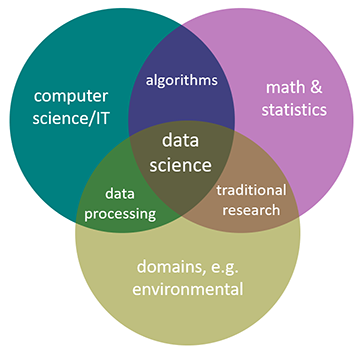
\includegraphics[width=0.75\linewidth]{img/EnvDataSci50pct} 

}

\caption{Environmental data science}\label{fig:indexEDS}
\end{figure}

\section{Environmental Data and Methods}\label{environmental-data-and-methods}

The methods needed for environmental research can include many things since environmental \emph{data} can include many things, including environmental measurements in space and time domains. \index{environmental data}

\begin{itemize}
\tightlist
\item
  data analysis and transformation methods

  \begin{itemize}
  \tightlist
  \item
    importing and other methods to create data frames
  \item
    reorganization and creation of fields
  \item
    filtering observations
  \item
    data joins
  \item
    reorganizing data, including pivots
  \end{itemize}
\item
  visualization

  \begin{itemize}
  \tightlist
  \item
    graphics
  \item
    maps
  \item
    imagery
  \end{itemize}
\item
  spatial analysis

  \begin{itemize}
  \tightlist
  \item
    vector and raster spatial analysis

    \begin{itemize}
    \tightlist
    \item
      spatial joins
    \item
      distance analysis
    \item
      overlay analysis
    \item
      terrain modeling
    \end{itemize}
  \item
    spatial statistics
  \item
    image analysis
  \end{itemize}
\item
  statistical summaries, tests and models

  \begin{itemize}
  \tightlist
  \item
    statistical summaries and visualization
  \item
    stratified/grouped summaries
  \item
    confirmatory statistical tests
  \item
    physical, statistical and machine learning models
  \item
    classification models
  \end{itemize}
\item
  temporal data and time series

  \begin{itemize}
  \tightlist
  \item
    analyzing and visualizing long-term environmental data
  \item
    analyzing and visualizing high-frequency data from loggers
  \end{itemize}
\end{itemize}

\section{Goals}\label{goals}

While the methodological reach of data science is very great, and the spectrum of environmental data is as well, our goal is to lay the foundation and provide useful introductory methods in the areas outlined above, but as a ``live'' book be able to extend into more advanced methods and provide a growing suite of research examples with associated data sets. We'll briefly explore some data mining methods that can be applied to so-called ``big data'' challenges, but our focus is on \textbf{exploratory data analysis} in general, applied to environmental data in \emph{space and time domains}. For clarity in understanding the methods and products, much of our data will be in fact be quite \emph{small}, derived from field-based environmental measurements where we can best understand how the data was collected, but these methods extend to much larger data sets. It will primarily be in the areas of time-series and imagery, where automated data capture and machine learning are employed, when we'll dip our toes into big data.

\subsection{Some definitions:}\label{some-definitions}

\index{machine learning}\textbf{Machine Learning}: \emph{building a model using training data in order to make predictions without being explicitly programmed to do so.} Related to artificial intelligence methods. Used in:

\begin{itemize}
\tightlist
\item
  image and imagery classification, including computer vision methods
\item
  statistical modeling
\item
  data mining
\end{itemize}

\index{data mining}\textbf{Data Mining}: \emph{discovering patterns in large data sets}

\begin{itemize}
\tightlist
\item
  databases collected by government agencies
\item
  imagery data from satellite, aerial (including drone) sensors
\item
  time-series data from long-term data records or high-frequency data loggers
\item
  methods may involve machine learning, artificial intelligence and computer vision
\end{itemize}

\index{big data}\textbf{Big Data}: \emph{data having a size or complexity too big to be processed effectively by traditional software}

\begin{itemize}
\tightlist
\item
  data with many cases or dimensions (including imagery)
\item
  many applications in environmental science due to the great expansion of automated environmental data capture in space and time domains
\item
  big data challenges exist across the spectrum of the environmental research process, from data capture, storage, sharing, visualization, querying
\end{itemize}

\textbf{Exploratory Data Analysis}: \emph{procedures for analyzing data, techniques for interpreting the results of such procedures, ways of structuring data to make its analysis easier}

\begin{itemize}
\tightlist
\item
  summarizing
\item
  restructuring
\item
  visualization
\end{itemize}

\section{Exploratory Data Analysis}\label{exploratory-data-analysis}

\index{exploratory data analysis}Just as \emph{exploration} is a part of what \emph{National Geographic} has long covered, it's an important part of geographic and environmental science research. \textbf{Exploratory data analysis} is exploration applied to data, and has grown as an alternative approach to traditional statistical analysis. This basic approach perhaps dates back to the work of Thomas Bayes in the eighteenth century, but Tukey (\citeproc{ref-tukey1962}{1962}) may have best articulated the basic goals of this approach in defining the ``data analysis'' methods he was promoting: ``Procedures for analyzing data, techniques for interpreting the results of such procedures, ways of planning the gathering of data to make its analysis easier, more precise or more accurate, and all the machinery and results of (mathematical) statistics which apply to analyzing data.'' Some years later Tukey (\citeproc{ref-tukey1977}{1977}) followed up with \emph{Exploratory Data Analysis}.

Exploratory data analysis (EDA) is an approach to analyzing data via summaries and graphics. The key word is \emph{exploratory}, and while one might view this in contrast to \emph{confirmatory} statistics, in fact they are highly complementary. The objectives of EDA include (a) suggesting hypotheses; (b) assessing assumptions on which inferences will be based; (c) selecting appropriate statistical tools; and (d) guiding further data collection. This philosophy led to the development of S at Bell Labs (led by John Chambers, 1976), then to R.

\section{Software and Data}\label{software-and-data}

First, we're going to use the R language, designed for statistical computing and graphics. It's not the only way to do data analysis -- Python is another important data science language -- but R with its statistical foundation is an important language for academic research, especially in the environmental sciences.

\begin{verbatim}
## [1] "This book was produced in RStudio using R version 4.6.1 (2026-06-24 ucrt)"
\end{verbatim}

For a start, you'll need to have R and \index{RStudio}RStudio installed, then you'll need to install various \index{packages}packages to support specific chapters and sections. Most of these are installed from the \url{https://cran.r-project.org/} site. You may want to go ahead and install all of the packages needed for the chapters through Chapter \ref{visualization}.

\begin{itemize}
\tightlist
\item
  In \textbf{Introduction to R} (Chapter \ref{introduction}), we will mostly use the base installation of R, with a few packages to provide data and enhanced table displays:

  \begin{itemize}
  \tightlist
  \item
    \texttt{igisci}
  \item
    \texttt{palmerpenguins}
  \item
    \texttt{DT}
  \item
    \texttt{knitr}
  \end{itemize}
\item
  In \textbf{Abstraction} (Chapter \ref{abstraction}) and \textbf{Transformation} (Chapter \ref{transformation}), we'll start making a lot of use of \emph{tidyverse} \ref{tidyverse} packages such as:

  \begin{itemize}
  \tightlist
  \item
    \texttt{ggplot2}
  \item
    \texttt{dplyr}
  \item
    \texttt{stringr}
  \item
    \texttt{tidyr}
  \item
    \texttt{lubridate}
  \end{itemize}
\item
  In \textbf{Visualization} (Chapter \ref{visualization}), we'll mostly use ggplot2, but also some specialized visualization packages such as:

  \begin{itemize}
  \tightlist
  \item
    \texttt{GGally}
  \end{itemize}
\item
  In \textbf{Spatial} (starting with Chapter \ref{spatial}), we'll add some spatial data, analysis and mapping packages. Note that these packages continue to be developed, especially \texttt{terra} and \texttt{tmap}, so we might want to look for updates when we get to it:

  \begin{itemize}
  \tightlist
  \item
    \texttt{sf}
  \item
    \texttt{terra}
  \item
    \texttt{tmap} (we won't use the CRAN version, but instead version 4 on github)
  \item
    \texttt{leaflet}
  \end{itemize}
\item
  In \textbf{Statistics and Modeling} (starting with Chapter \ref{statistics}), no additional packages are needed, as we can rely on base R's rich statistical methods and ggplot2's visualization.
\item
  In \textbf{Time Series} (Chapter \ref{ts}), we'll find a few other packages handy:

  \begin{itemize}
  \tightlist
  \item
    \texttt{xts} (Extensible Time Series)
  \item
    \texttt{forecast} (for a few useful functions like a moving average)
  \end{itemize}
\end{itemize}

\index{installation}And there will certainly be other packages we'll explore along the way, so you'll want to install them when you first need them, which will typically be when you first see a \texttt{library()} call in the code, or possibly when a function is prefaced with the package name, something like \texttt{dplyr::select()}, or maybe when R raises an error that it can't find a function you've called or that the package isn't installed. One of the earliest we'll need is the suite of packages in the ``tidyverse'' (Wickham and Grolemund (\citeproc{ref-wickham2016r}{2016})), which includes some of the ones listed above: \texttt{ggplot2}, \texttt{dplyr}, \texttt{stringr}, and \texttt{tidyr}. You can install these individually, or all at once with:

\begin{verbatim}
install.packages("tidyverse")
\end{verbatim}

\index{install.packages}This is usually done from the console in RStudio and not included in an R script or markdown document, since you don't want to be installing the package over and over again. You can also respond to a prompt from RStudio when it detects a package called in a script you open that you don't have installed.

From time to time, you'll want to update your installed packages, and that usually happens when something doesn't work and maybe the dependencies of one package on another gets broken with a change in a package. Fortunately, in the R world, especially at the main repository at CRAN, there's a lot of effort put into making sure packages work together, so usually there are no surprises if you're using the most current versions. \emph{Note that there can be exceptions to this, and occasionally new package versions will create problems with other packages due to inter-package dependencies and the introduction of functions with names that duplicate other packages. The packages installed for this book were current as of that version of R, but new package versions may occasionally introduce errors.}

Once a package like \texttt{dplyr} is installed, you can access all of its functions and data by adding a library call, like \ldots{}

\begin{Shaded}
\begin{Highlighting}[]
\FunctionTok{library}\NormalTok{(dplyr)}
\end{Highlighting}
\end{Shaded}

\ldots{} which you \emph{will} want to include in your code, or to provide access to multiple libraries in the tidyverse, you can use \texttt{library(tidyverse)}. Alternatively, if you're only using maybe one function out of an installed package, you can call that function with the \texttt{::} separator, like \texttt{dplyr::select()}. This method has another advantage in avoiding problems with duplicate names -- and for instance we'll generally call \texttt{dplyr::select()} this way.

\textbf{Addenda:} There are other methods we could look at, as well as case studies and expansions of methods we will look at. So we've also created an \emph{Environmental Data Science Addenda} at \url{https://bookdown.org/igisc/EnvDataSciAddenda/}.

\subsection{Data}\label{data}

We'll be using data from various sources, including data on CRAN like the code packages above which you install the same way -- so use \texttt{install.packages("palmerpenguins")}.

\index{data}We've also created a repository on GitHub that includes data we've developed in the Institute for Geographic Information Science (iGISc) at SFSU, and you'll need to install that package a slightly different way.

\begin{center}
\includegraphics[width=0.33\linewidth]{img/IGIScSFSU281200} \end{center}

GitHub packages \index{GitHub packages}require a bit more work on the user's part since we need to first install \texttt{remotes}\footnote{Note: you can also use \texttt{devtools} instead of \texttt{remotes} if you have that installed. They do the same thing; \texttt{remotes} is a subset of \texttt{devtools}. If you see a message about Rtools, you can ignore it since that is only needed for building tools from C++ and things like that.}, then use that to install the GitHub data package:

\begin{Shaded}
\begin{Highlighting}[]
\FunctionTok{install.packages}\NormalTok{(}\StringTok{"remotes"}\NormalTok{)}
\NormalTok{remotes}\SpecialCharTok{::}\FunctionTok{install\_github}\NormalTok{(}\StringTok{"iGISc/igisci"}\NormalTok{)}
\end{Highlighting}
\end{Shaded}

\index{igisci}Then you can access it just like other built-in data by including:

\begin{Shaded}
\begin{Highlighting}[]
\FunctionTok{library}\NormalTok{(igisci)}
\end{Highlighting}
\end{Shaded}

To see what's in it, you'll see the various datasets listed in:

\begin{verbatim}
data(package="igisci")
\end{verbatim}

This creates a view of the data in the \texttt{igisci} packages, which is useful in the RStudio environment. One of the functions also built into the \texttt{igisci} package creates a \emph{data frame} of the data in that package. We'll be learning about data frames in the next chapter, but basically it's a simple rectangular database with rows and columns, where columns are variables and rows are sets of observations. That function is \texttt{exfiles()} which you can call once you've loaded the \texttt{igisci} library as we've just done. To create a data frame we'll call \texttt{igisciData} we'd assign it \texttt{exfiles()}.

\begin{Shaded}
\begin{Highlighting}[]
\FunctionTok{library}\NormalTok{(igisci)}
\NormalTok{igisciData }\OtherTok{=} \FunctionTok{exfiles}\NormalTok{()}
\end{Highlighting}
\end{Shaded}

Then we can view it in the RStudio interface with:

\begin{Shaded}
\begin{Highlighting}[]
\FunctionTok{View}\NormalTok{(igisciData)}
\end{Highlighting}
\end{Shaded}

We can display the contents of a data frame in various ways, one simple way using the \texttt{display} function of the \texttt{insight} package, so after we've installed \texttt{insight} with \texttt{install.packages("insight")}, we can use \texttt{display} with our newly created data frame:

\begin{Shaded}
\begin{Highlighting}[]
\FunctionTok{library}\NormalTok{(insight)}
\FunctionTok{display}\NormalTok{(igisciData)}
\end{Highlighting}
\end{Shaded}

{\def\LTcaptype{none} % do not increment counter
\begin{longtable}[]{@{}
  >{\raggedright\arraybackslash}p{(\linewidth - 6\tabcolsep) * \real{0.0976}}
  >{\raggedleft\arraybackslash}p{(\linewidth - 6\tabcolsep) * \real{0.3659}}
  >{\raggedleft\arraybackslash}p{(\linewidth - 6\tabcolsep) * \real{0.4553}}
  >{\raggedright\arraybackslash}p{(\linewidth - 6\tabcolsep) * \real{0.0813}}@{}}
\toprule\noalign{}
\begin{minipage}[b]{\linewidth}\raggedright
dir
\end{minipage} & \begin{minipage}[b]{\linewidth}\raggedleft
file
\end{minipage} & \begin{minipage}[b]{\linewidth}\raggedleft
path
\end{minipage} & \begin{minipage}[b]{\linewidth}\raggedright
type
\end{minipage} \\
\midrule\noalign{}
\endhead
\bottomrule\noalign{}
\endlastfoot
airquality & CES4 Final Shapefile.shp & ex(`airquality/CES4 Final Shapefile.shp') & shapefile \\
airquality & Pollution by type US 1970 to 2016.xlsx & ex(`airquality/Pollution by type US 1970 to 2016.xlsx') & xls \\
BayArea & BayAreaCounties.shp & ex(`BayArea/BayAreaCounties.shp') & shapefile \\
BayArea & BayAreaTracts.shp & ex(`BayArea/BayAreaTracts.shp') & shapefile \\
BayArea & BayArea\_hillsh.tif & ex(`BayArea/BayArea\_hillsh.tif') & TIFF \\
CA & CA\_counties.shp & ex(`CA/CA\_counties.shp') & shapefile \\
CA & CAfreeways.shp & ex(`CA/CAfreeways.shp') & shapefile \\
CA & ca\_elev.tif & ex(`CA/ca\_elev.tif') & TIFF \\
CA & ca\_elev\_WGS84.tif & ex(`CA/ca\_elev\_WGS84.tif') & TIFF \\
CA & ca\_hillsh\_WGS84.tif & ex(`CA/ca\_hillsh\_WGS84.tif') & TIFF \\
CA & CA\_ClimateNormals.csv & ex(`CA/CA\_ClimateNormals.csv') & CSV \\
CA & CA\_MdInc.csv & ex(`CA/CA\_MdInc.csv') & CSV \\
CA & CA\_MdInc\_Tr\_2016.csv & ex(`CA/CA\_MdInc\_Tr\_2016.csv') & CSV \\
CA & CDC\_health\_data\_by\_Tract\_CA\_2018\_release.csv & ex(`CA/CDC\_health\_data\_by\_Tract\_CA\_2018\_release.csv') & CSV \\
eucoak & eucoak\_sites.csv & ex(`eucoak/eucoak\_sites.csv') & CSV \\
eucoak & eucoakrainfallrunoffTDR.csv & ex(`eucoak/eucoakrainfallrunoffTDR.csv') & CSV \\
eucoak & eucoaksediment.csv & ex(`eucoak/eucoaksediment.csv') & CSV \\
eucoak & eucoakSites.csv & ex(`eucoak/eucoakSites.csv') & CSV \\
eucoak & eucoakSites.csv.xml & ex(`eucoak/eucoakSites.csv.xml') & CSV \\
eucoak & REMOVEeucoak\_sites.csv & ex(`eucoak/REMOVEeucoak\_sites.csv') & CSV \\
eucoak & tidy\_eucoak.csv & ex(`eucoak/tidy\_eucoak.csv') & CSV \\
fish & fishdata.csv & ex(`fish/fishdata.csv') & CSV \\
gully & gullyGrowth.csv & ex(`gully/gullyGrowth.csv') & CSV \\
litter & ConcentrationReport.csv & ex(`litter/ConcentrationReport.csv') & CSV \\
marbles & co2july95.shp & ex(`marbles/co2july95.shp') & shapefile \\
marbles & geology.shp & ex(`marbles/geology.shp') & shapefile \\
marbles & gps97.shp & ex(`marbles/gps97.shp') & shapefile \\
marbles & samples.shp & ex(`marbles/samples.shp') & shapefile \\
marbles & streams.shp & ex(`marbles/streams.shp') & shapefile \\
marbles & trails.shp & ex(`marbles/trails.shp') & shapefile \\
marbles & elev.tif & ex(`marbles/elev.tif') & TIFF \\
marbles & bulkdens970901.csv & ex(`marbles/bulkdens970901.csv') & CSV \\
marbles & resurgenceData.csv & ex(`marbles/resurgenceData.csv') & CSV \\
marbles & resurgenceDataVariables.csv & ex(`marbles/resurgenceDataVariables.csv') & CSV \\
marbles & soilCO2\_97.alldata.csv & ex(`marbles/soilCO2\_97.alldata.csv') & CSV \\
marbles & soilCO2\_97.csv & ex(`marbles/soilCO2\_97.csv') & CSV \\
marbles & soilCO2\_97\_site\_descriptions.csv & ex(`marbles/soilCO2\_97\_site\_descriptions.csv') & CSV \\
marbles & soilCO2\_97\_variables.csv & ex(`marbles/soilCO2\_97\_variables.csv') & CSV \\
marbles & soilCO2\_sites97\_gcs.csv & ex(`marbles/soilCO2\_sites97\_gcs.csv') & CSV \\
marbles & resurgenceData.xlsx & ex(`marbles/resurgenceData.xlsx') & xls \\
marbles & soilCO2\_97.xlsx & ex(`marbles/soilCO2\_97.xlsx') & xls \\
meadows & SoilVegSamples.csv & ex(`meadows/SoilVegSamples.csv') & CSV \\
meadows & XSptsNDVI.csv & ex(`meadows/XSptsNDVI.csv') & CSV \\
meadows & XSptsPheno.csv & ex(`meadows/XSptsPheno.csv') & CSV \\
meadows & LoneyMeadow\_30minCO2fluxes\_Geog604.xls & ex(`meadows/LoneyMeadow\_30minCO2fluxes\_Geog604.xls') & xls \\
meadows & RCV\_carbon\_flux\_data.xlsx & ex(`meadows/RCV\_carbon\_flux\_data.xlsx') & xls \\
Nile & NilePoints.csv & ex(`Nile/NilePoints.csv') & CSV \\
penguins & sat\_table\_splash.csv & ex(`penguins/sat\_table\_splash.csv') & CSV \\
RCVimagery & RCVcrop.shp & ex(`RCVimagery/RCVcrop.shp') & shapefile \\
RCVimagery & train\_points.shp & ex(`RCVimagery/train\_points.shp') & shapefile \\
RCVimagery & train\_polys7.shp & ex(`RCVimagery/train\_polys7.shp') & shapefile \\
RCVimagery & train\_polys9.shp & ex(`RCVimagery/train\_polys9.shp') & shapefile \\
SanPedro & roads.shp & ex(`SanPedro/roads.shp') & shapefile \\
SanPedro & slideCentroids.shp & ex(`SanPedro/slideCentroids.shp') & shapefile \\
SanPedro & SPCWatershed.shp & ex(`SanPedro/SPCWatershed.shp') & shapefile \\
SanPedro & streams.shp & ex(`SanPedro/streams.shp') & shapefile \\
SanPedro & trails.shp & ex(`SanPedro/trails.shp') & shapefile \\
SanPedro & dem.tif & ex(`SanPedro/dem.tif') & TIFF \\
SanPedro & SI.tif & ex(`SanPedro/SI.tif') & TIFF \\
SanPedro & SanPedroCreekBacterialCounts.csv & ex(`SanPedro/SanPedroCreekBacterialCounts.csv') & CSV \\
SFmarine & cordell\_bank.shp & ex(`SFmarine/cordell\_bank.shp') & shapefile \\
SFmarine & isobath\_200.shp & ex(`SFmarine/isobath\_200.shp') & shapefile \\
SFmarine & mainland.shp & ex(`SFmarine/mainland.shp') & shapefile \\
SFmarine & Sanctuaries.shp & ex(`SFmarine/Sanctuaries.shp') & shapefile \\
SFmarine & sefi.shp & ex(`SFmarine/sefi.shp') & shapefile \\
SFmarine & transects.shp & ex(`SFmarine/transects.shp') & shapefile \\
SFmarine & bd200m\_v2i.tif & ex(`SFmarine/bd200m\_v2i.tif') & TIFF \\
SFmarine & Transects\_Metadata.xls & ex(`SFmarine/Transects\_Metadata.xls') & xls \\
SFmarine & TransectsData.xls & ex(`SFmarine/TransectsData.xls') & xls \\
sierra & CA\_places.shp & ex(`sierra/CA\_places.shp') & shapefile \\
sierra & 908277.csv & ex(`sierra/908277.csv') & CSV \\
sierra & sagehen\_dv.csv & ex(`sierra/sagehen\_dv.csv') & CSV \\
sierra & Sierra2LassenData.csv & ex(`sierra/Sierra2LassenData.csv') & CSV \\
sierra & sierraClimate.csv & ex(`sierra/sierraClimate.csv') & CSV \\
sierra & sierraData.csv & ex(`sierra/sierraData.csv') & CSV \\
sierra & sierraFeb.csv & ex(`sierra/sierraFeb.csv') & CSV \\
sierra & sierraFebShort.csv & ex(`sierra/sierraFebShort.csv') & CSV \\
sierra & sierraStations.csv & ex(`sierra/sierraStations.csv') & CSV \\
SinkingCove & CaveEntrances.shp & ex(`SinkingCove/CaveEntrances.shp') & shapefile \\
SinkingCove & caves.shp & ex(`SinkingCove/caves.shp') & shapefile \\
SinkingCove & Contour10.shp & ex(`SinkingCove/Contour10.shp') & shapefile \\
SinkingCove & geology.shp & ex(`SinkingCove/geology.shp') & shapefile \\
SinkingCove & DEM\_SinkingCoveGCS.tif & ex(`SinkingCove/DEM\_SinkingCoveGCS.tif') & TIFF \\
SinkingCove & DEM\_SinkingCoveUTM.tif & ex(`SinkingCove/DEM\_SinkingCoveUTM.tif') & TIFF \\
SinkingCove & SinkingCoveSites.csv & ex(`SinkingCove/SinkingCoveSites.csv') & CSV \\
SinkingCove & SinkingCoveWaterChem.xlsx & ex(`SinkingCove/SinkingCoveWaterChem.xlsx') & xls \\
streams & streams.csv & ex(`streams/streams.csv') & CSV \\
TRI & BayAreaCounties.shp & ex(`TRI/BayAreaCounties.shp') & shapefile \\
TRI & BayAreaTracts.shp & ex(`TRI/BayAreaTracts.shp') & shapefile \\
TRI & BayArea\_hillsh.tif & ex(`TRI/BayArea\_hillsh.tif') & TIFF \\
TRI & CA\_MdInc.csv & ex(`TRI/CA\_MdInc.csv') & CSV \\
TRI & CA\_MdInc\_Tr\_2016.csv & ex(`TRI/CA\_MdInc\_Tr\_2016.csv') & CSV \\
TRI & CDC\_health\_data\_by\_Tract\_CA\_2018\_release.csv & ex(`TRI/CDC\_health\_data\_by\_Tract\_CA\_2018\_release.csv') & CSV \\
TRI & TRI\_1987\_BaySites.csv & ex(`TRI/TRI\_1987\_BaySites.csv') & CSV \\
TRI & TRI\_1987\_CA.csv & ex(`TRI/TRI\_1987\_CA.csv') & CSV \\
TRI & TRI\_1997\_CA.csv & ex(`TRI/TRI\_1997\_CA.csv') & CSV \\
TRI & TRI\_2007\_CA.csv & ex(`TRI/TRI\_2007\_CA.csv') & CSV \\
TRI & TRI\_2017\_CA.csv & ex(`TRI/TRI\_2017\_CA.csv') & CSV \\
ts & LoneyMeadow\_30minCO2fluxes\_Geog604.xls & ex(`ts/LoneyMeadow\_30minCO2fluxes\_Geog604.xls') & xls \\
ts & SolarRad\_Temp.xls & ex(`ts/SolarRad\_Temp.xls') & xls \\
US & peaks.shp & ex(`US/peaks.shp') & shapefile \\
US & US\_states\_Simp.shp & ex(`US/US\_states\_Simp.shp') & shapefile \\
US & W\_States.shp & ex(`US/W\_States.shp') & shapefile \\
US & USDOE\_FuelEfficiency2022.xlsx & ex(`US/USDOE\_FuelEfficiency2022.xlsx') & xls \\
\end{longtable}
}

The data shown in the \texttt{exfiles()} result includes raw data files like text files, shape files and other things that we can read in with the various tools we'll learn about that read them, and most of the data we'll use from \texttt{igisci} will be accessed this way.

The package also includes some data that are directly accessible, like the \texttt{CA\_counties} map of
California counties shown in Figure \ref{fig:indexCAcounties} built as \texttt{sf} feature data. We'll be looking at the \texttt{sf} (Simple Features) package later in the Spatial section of the book, but seeing \texttt{library(sf)}, this is one place where you'd need to have installed another package, with \texttt{install.packages("sf")}.

\begin{Shaded}
\begin{Highlighting}[]
\FunctionTok{library}\NormalTok{(tidyverse); }\FunctionTok{library}\NormalTok{(igisci); }\FunctionTok{library}\NormalTok{(sf)}
\FunctionTok{ggplot}\NormalTok{(}\AttributeTok{data=}\NormalTok{CA\_counties) }\SpecialCharTok{+} \FunctionTok{geom\_sf}\NormalTok{()}
\end{Highlighting}
\end{Shaded}

\begin{figure}

{\centering 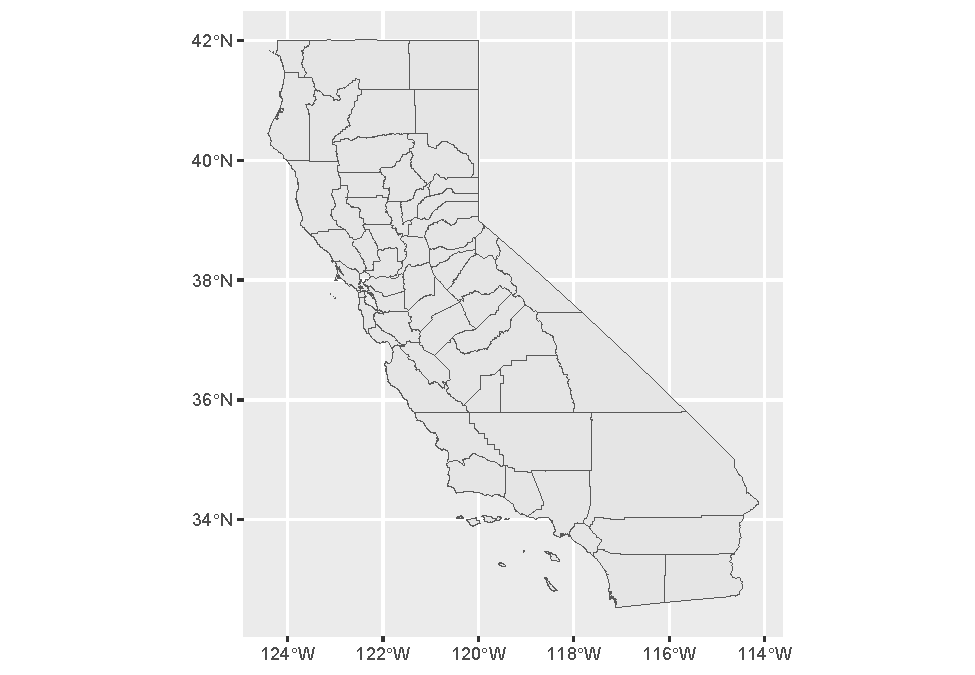
\includegraphics[width=0.75\linewidth]{EnvDataScience_files/figure-latex/indexCAcounties-1} 

}

\caption{California counties simple features data in igisci package}\label{fig:indexCAcounties}
\end{figure}

The package datasets can be used directly as \texttt{sf} data or data frames. And similarly to functions, you can access the (previously installed) data set by prefacing with \texttt{igisci::} this way, without having to load the library. This might be useful in a one-off operation:

\begin{Shaded}
\begin{Highlighting}[]
\FunctionTok{mean}\NormalTok{(igisci}\SpecialCharTok{::}\NormalTok{sierraFeb}\SpecialCharTok{$}\NormalTok{LATITUDE)}
\end{Highlighting}
\end{Shaded}

\begin{verbatim}
## [1] 38.3192
\end{verbatim}

Raw data such as \texttt{.csv} files can also be read from the \texttt{extdata} folder that is installed on your computer when you install the package, using code such as:

\begin{verbatim}
csvPath <- system.file("extdata","TRI/TRI_1987_BaySites.csv", package="igisci")
TRI87 <- read_csv(csvPath)
\end{verbatim}

or something similar for shapefiles, such as:

\begin{verbatim}
shpPath <- system.file("extdata","marbles/trails.shp", package="igisci")
trails <- st_read(shpPath)
\end{verbatim}

And we'll find that including most of the above arcanity in a function will help. We'll look at functions later, but here's a function that we'll use a lot for setting up reading data from the extdata folder:

\begin{verbatim}
ex <- function(dta){system.file("extdata",dta,package="igisci")}
\end{verbatim}

And this \texttt{ex()}function is needed so often that it's installed in the \texttt{igisci} package, so if you have \texttt{library(igisci)} in effect, you can just use it like this:

\begin{verbatim}
trails <- st_read(ex("marbles/trails.shp"))
\end{verbatim}

But how do we see what's in the \texttt{extdata} folder? We can't use the \texttt{data()} function, so we would have to dig for the folder where the igisci package gets installed, which is buried pretty deeply in your user profile. So I wrote another function \texttt{exfiles()} that creates a data frame showing all of the files and the paths to use. In RStudio you could access it with \texttt{View(exfiles())} or we could use a datatable (you'll need to have installed ``DT''). You can use the path using the \texttt{ex()} function with any function that needs it to read data, like \texttt{read.csv(ex(\textquotesingle{}CA/CA\_ClimateNormals.csv\textquotesingle{}))}, or just enter that \texttt{ex()} call in the console like \texttt{ex(\textquotesingle{}CA/CA\_ClimateNormals.csv\textquotesingle{})} to display where on your computer the installed data reside.

\begin{Shaded}
\begin{Highlighting}[]
\NormalTok{DT}\SpecialCharTok{::}\FunctionTok{datatable}\NormalTok{(}\FunctionTok{exfiles}\NormalTok{(), }\AttributeTok{options=}\FunctionTok{list}\NormalTok{(}\AttributeTok{scrollX=}\NormalTok{T), }\AttributeTok{rownames=}\NormalTok{F)}
\end{Highlighting}
\end{Shaded}

\begin{center}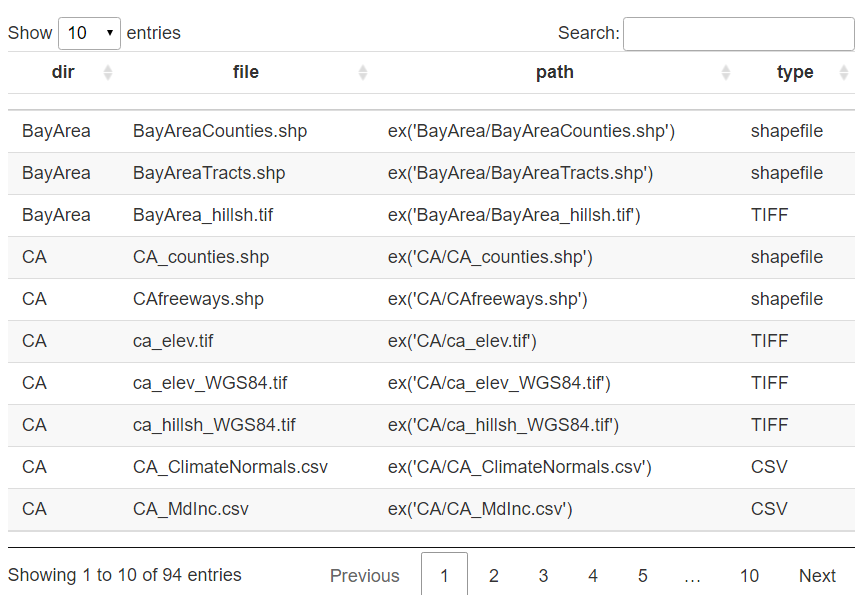
\includegraphics[width=1\linewidth]{img/exfilesDT} \end{center}

\begin{center}\rule{0.5\linewidth}{0.5pt}\end{center}

\section{Acknowledgements}\label{acknowledgements}

This book was immensely aided by extensive testing by students in San Francisco State's GEOG 604/704 \emph{Environmental Data Science} class, including specific methodological contributions from some of the students and a contributed data wrangling exercise by one from the first offering (Josh von Nonn) in Chapter 5. Thanks to Andrew Oliphant, Chair of the Department of Geography and Environment, for supporting the class (as long as I included time series) and then came through with some great data sets from eddy covariance flux towers as well as guest lectures. Many thanks to Adam Davis, California Energy Commission, for suggestions on R spatial methods and package development, among other things in the R world. Thanks to Anna Studwell, recent Associate Director of the IGISc, for ideas on statistical modeling of birds and marine environments, and the nice water-color for the front cover. And a lot of thanks goes to Nancy Wilkinson, who put up with my obsessing on R coding puzzles at all hours and pretended to be impressed with what you can do with R Markdown.

\begin{center}\rule{0.5\linewidth}{0.5pt}\end{center}

\emph{Introduction to Environmental Data Science} © Jerry D. Davis, ORCID 0000-0002-5369-1197, Institute for Geographic Information Science, San Francisco State University, all rights reserved.

Published as Davis JD (2022). \emph{Introduction to Environmental Data Science}. Chapman \& Hall/CRC Data Science Series. ISBN: 9781032322186. Available at Amazon and Routledge in hard copy and Kindle versions.

\begin{center}\rule{0.5\linewidth}{0.5pt}\end{center}

{\emph{Introduction to Environmental Data Science}} by Jerry Davis is licensed under a Creative Commons Attribution 4.0 International License.

Cover art ``Dandelion fluff -- Ephemeral stalk sheds seeds to the universe'' by Anna Studwell.

\part{Exploratory Data Analysis}\label{part-exploratory-data-analysis}

\chapter{Introduction to R}\label{introduction}

This section lays the foundation for exploratory data analysis using the R language and packages especially within the tidyverse. This foundation progresses through:

\begin{itemize}
\tightlist
\item
  Introduction : An introduction to the R language
\item
  Abstraction : Exploration of data via reorganization using \texttt{dplyr} and other packages in the tidyverse (Chapter \ref{abstraction})
\item
  Visualization : Adding visual tools to enhance our data exploration (Chapter \ref{visualization})
\item
  Transformation : Reorganizing our data with pivots and data joins (Chapter \ref{transformation})
\end{itemize}

In this chapter we'll introduce the R language, using RStudio to explore its basic data types, structures, functions and programming methods in base R. We're assuming you're either new to R or need a refresher. Later chapters will add packages that extend what you can do with base R for data abstraction, transformation, and visualization, then explore the spatial world, statistical models, and time series applied to environmental research.

The following code illustrates a few of the methods we'll explore in this chapter:

\begin{Shaded}
\begin{Highlighting}[]
\NormalTok{tC }\OtherTok{\textless{}{-}} \FunctionTok{c}\NormalTok{(}\FloatTok{10.7}\NormalTok{, }\FloatTok{9.7}\NormalTok{, }\FloatTok{7.7}\NormalTok{, }\FloatTok{9.2}\NormalTok{, }\FloatTok{7.3}\NormalTok{)}
\NormalTok{elev }\OtherTok{\textless{}{-}} \FunctionTok{c}\NormalTok{(}\DecValTok{52}\NormalTok{, }\DecValTok{394}\NormalTok{, }\DecValTok{510}\NormalTok{, }\DecValTok{564}\NormalTok{, }\DecValTok{725}\NormalTok{)}
\NormalTok{lat }\OtherTok{\textless{}{-}} \FunctionTok{c}\NormalTok{(}\FloatTok{39.52}\NormalTok{, }\FloatTok{38.91}\NormalTok{, }\FloatTok{37.97}\NormalTok{, }\FloatTok{38.70}\NormalTok{, }\FloatTok{39.09}\NormalTok{)}
\NormalTok{elevft }\OtherTok{\textless{}{-}} \FunctionTok{round}\NormalTok{(elev }\SpecialCharTok{/} \FloatTok{0.3048}\NormalTok{)}
\NormalTok{deg }\OtherTok{\textless{}{-}} \FunctionTok{as.integer}\NormalTok{(lat)}
\NormalTok{min }\OtherTok{\textless{}{-}} \FunctionTok{as.integer}\NormalTok{((lat}\SpecialCharTok{{-}}\NormalTok{deg) }\SpecialCharTok{*} \DecValTok{60}\NormalTok{)}
\NormalTok{sec }\OtherTok{\textless{}{-}} \FunctionTok{round}\NormalTok{((lat}\SpecialCharTok{{-}}\NormalTok{deg}\SpecialCharTok{{-}}\NormalTok{min}\SpecialCharTok{/}\DecValTok{60}\NormalTok{)}\SpecialCharTok{*}\DecValTok{3600}\NormalTok{)}
\NormalTok{sierradata }\OtherTok{\textless{}{-}} \FunctionTok{cbind}\NormalTok{(tC, elev, elevft, lat, deg, min, sec)}
\NormalTok{mydata }\OtherTok{\textless{}{-}} \FunctionTok{as.data.frame}\NormalTok{(sierradata)}
\NormalTok{mydata}
\end{Highlighting}
\end{Shaded}

\begin{verbatim}
##     tC elev elevft   lat deg min sec
## 1 10.7   52    171 39.52  39  31  12
## 2  9.7  394   1293 38.91  38  54  36
## 3  7.7  510   1673 37.97  37  58  12
## 4  9.2  564   1850 38.70  38  42   0
## 5  7.3  725   2379 39.09  39   5  24
\end{verbatim}

\textbf{RStudio}

\index{RStudio}If you're new to RStudio, or would like to learn more about using it, there are plenty of resources you can access to learn more about using it. As with many of the major packages we'll explore, there's even a cheat sheet: \url{https://www.rstudio.com/resources/cheatsheets/}. Have a look at this cheat sheet while you have RStudio running, and use it to learn about some of its different components:

\begin{itemize}
\tightlist
\item
  The \textbf{Console}, where you'll enter short lines of code, install packages, and get help on functions. Messages created from running code will also be displayed here. There are other tabs in this area (e.g.~Terminal, R Markdown) we may explore a bit, but mostly we'll use the console.
\item
  The \textbf{Source Editor}, where you'll write full R scripts and R Markdown documents. You should get used to writing complete scripts and R Markdown documents as we go through the book.
\item
  Various \textbf{Tab Panes} such as the \textbf{Environment} pane, where you can explore what scalars and more complex objects contain.
\item
  The \textbf{Plots} pane in the lower right for static plots (graphs and maps that aren't interactive), which also lets you see a listing of \textbf{Files}, or \textbf{View} interactive maps and maps.
\end{itemize}

\section{Data Objects}\label{data-objects}

As with all programming languages, R works with \emph{data} and since it's an object-oriented language, these are \index{data objects}\emph{data objects}. Data objects can range from the most basic type -- the \emph{scalar} which holds one value, like a number or text -- to everything from an array of values to spatial data for mapping or a time series of data.

\subsection{Scalars and assignment}\label{scalars-and-assignment}

We'll be looking at a variety of types of data objects, but \index{scalars}scalars are the most basic type, holding individual values, so we'll start with it. Every computer language, like in math, stores values by assigning them constants or results of expressions. These are often called ``variables,'' but we'll be using that name to refer to a column of data stored in a data frame, which we'll look at later in this chapter. R uses a lot of objects, and not all are data objects; we'll also create functions \ref{functions-writing}, a type of object that does something (runs the function code you've defined for it) with what you provide it.

To create a scalar (or other data objects), we'll use the most common type of statement, the \index{assignment statement}\emph{assignment statement}, that takes an \index{expression}\emph{expression} and assigns it to a new data object that we'll name. The \emph{class} of that data object is determined by the class of the expression provided, and that expression might be something as simple as a \index{constant}\emph{constant} like a number or a character string of text. Here's an example of a very basic assignment statement that assigns the value of a constant \texttt{5} to a new scalar \texttt{x}:

\texttt{x\ \textless{}-\ 5}

Note that this uses the assignment operator \texttt{\textless{}-} that is standard for R. You can also use \texttt{=} as most languages do (and I sometimes do), but we'll use \texttt{=} for other types of assignments.

All object names must start with a letter, have no spaces, and must not use any names that are built into the R language or used in package libraries, such as reserved words like \texttt{for} or function names like \texttt{log}. Object names are case-sensitive (which you'll probably discover at some point by typing in something wrong and getting an error).

\begin{Shaded}
\begin{Highlighting}[]
\NormalTok{x }\OtherTok{\textless{}{-}} \DecValTok{5}
\NormalTok{y }\OtherTok{\textless{}{-}} \DecValTok{8}
\NormalTok{Longitude }\OtherTok{\textless{}{-}} \SpecialCharTok{{-}}\FloatTok{122.4}
\NormalTok{Latitude }\OtherTok{\textless{}{-}} \FloatTok{37.8}
\NormalTok{my\_name }\OtherTok{\textless{}{-}} \StringTok{"Inigo Montoya"}
\end{Highlighting}
\end{Shaded}

To check the value of a data object, you can just enter the name in the console, or even in a script or code chunk.

\begin{Shaded}
\begin{Highlighting}[]
\NormalTok{x}
\end{Highlighting}
\end{Shaded}

\begin{verbatim}
## [1] 5
\end{verbatim}

\begin{Shaded}
\begin{Highlighting}[]
\NormalTok{y}
\end{Highlighting}
\end{Shaded}

\begin{verbatim}
## [1] 8
\end{verbatim}

\begin{Shaded}
\begin{Highlighting}[]
\NormalTok{Longitude}
\end{Highlighting}
\end{Shaded}

\begin{verbatim}
## [1] -122.4
\end{verbatim}

\begin{Shaded}
\begin{Highlighting}[]
\NormalTok{Latitude}
\end{Highlighting}
\end{Shaded}

\begin{verbatim}
## [1] 37.8
\end{verbatim}

\begin{Shaded}
\begin{Highlighting}[]
\NormalTok{my\_name}
\end{Highlighting}
\end{Shaded}

\begin{verbatim}
## [1] "Inigo Montoya"
\end{verbatim}

This is counter to the way printing out values commonly works in other programming languages, and you will need to know how this method works as well because you will want to use your code to develop tools that accomplish things, and there are also limitations to what you can see by just naming objects.

To see the values of objects in programming mode, you can also use the \index{print}\texttt{print()} function (but we rarely do); or to concatenate character string output, use \index{paste}\texttt{paste()} or \index{paste0}\texttt{paste0}.

\begin{Shaded}
\begin{Highlighting}[]
\FunctionTok{print}\NormalTok{(x)}
\FunctionTok{paste0}\NormalTok{(}\StringTok{"My name is "}\NormalTok{, my\_name, }\StringTok{". You killed my father. Prepare to die."}\NormalTok{)}
\end{Highlighting}
\end{Shaded}

Numbers concatenated with character strings are converted to characters.

\begin{Shaded}
\begin{Highlighting}[]
\FunctionTok{paste0}\NormalTok{(}\FunctionTok{paste}\NormalTok{(}\StringTok{"The Ultimate Answer to Life"}\NormalTok{, }\StringTok{"The Universe"}\NormalTok{, }
             \StringTok{"and Everything is ... "}\NormalTok{, }\AttributeTok{sep=}\StringTok{", "}\NormalTok{),}\DecValTok{42}\NormalTok{,}\StringTok{"!"}\NormalTok{)}
\end{Highlighting}
\end{Shaded}

\begin{Shaded}
\begin{Highlighting}[]
\FunctionTok{paste}\NormalTok{(}\StringTok{"The location is latitude"}\NormalTok{, Latitude, }\StringTok{"longitude"}\NormalTok{, Longitude)}
\end{Highlighting}
\end{Shaded}

\begin{verbatim}
## [1] "The location is latitude 37.8 longitude -122.4"
\end{verbatim}

Review the code above and what it produces. Without looking it up, what's the difference between \texttt{paste()} and \texttt{paste0()}?

\begin{quote}
We'll use \index{paste0() for long file paths}\texttt{paste0()} a lot in this book to deal with long file paths which create problems for the printed/pdf version of this book, basically extending into the margins. Breaking the path into multiple strings and then combining them with \texttt{paste0()} is one way to handle them. For instance, in the Imagery and Classification Models chapter, the Sentinel2 imagery is provided in a very long file path. So here's how we use \texttt{paste0()} to recombine after breaking up the path, and we then take it one more step and build out the full path to the 20 m imagery subset.
\end{quote}

\begin{Shaded}
\begin{Highlighting}[]
\NormalTok{imgFolder }\OtherTok{\textless{}{-}} \FunctionTok{paste0}\NormalTok{(}\StringTok{"S2A\_MSIL2A\_20210628T184921\_N0300\_R113\_T10TGK\_20210628T230915."}\NormalTok{,}
                    \StringTok{"SAFE/GRANULE/L2A\_T10TGK\_A031427\_20210628T185628"}\NormalTok{)}
\NormalTok{img20mFolder }\OtherTok{\textless{}{-}} \FunctionTok{paste0}\NormalTok{(}\StringTok{"\textasciitilde{}/sentinel2/"}\NormalTok{,imgFolder,}\StringTok{"/IMG\_DATA/R20m"}\NormalTok{)}
\end{Highlighting}
\end{Shaded}

\section{Functions}\label{functions}

Just as in regular mathematics, R makes a lot of use of \index{functions}\emph{functions} that accept an input and create an output:

\begin{verbatim}
log10(100)
log(exp(5))
cos(pi)
sin(90 * pi/180)
\end{verbatim}

But functions can be much more than numerical ones, and R functions can return a lot of different data objects. You'll find that most of your work will involve functions, from those in base R to a wide variety in packages you'll be adding. You will likely have already used the \texttt{install.packages()} and \texttt{library()} functions that add in an array of other functions.

Later in this chapter, we'll also learn how to \emph{write our own functions}, a capability that is easy to accomplish and also gives you a sense of what developing your own package might be like.

\index{arithmetic operators}\textbf{Arithmetic operators} There are, of course, all the normal arithmetic operators (that are actually functions) like plus \texttt{+} and minus \texttt{-} or the key-stroke approximations of multiply \texttt{*} and divide \texttt{/} operators. You're probably familiar with these approximations from using equations in Excel if not in some other programming language you may have learned. These operators look a bit different from how they'd look when creating a nicely formatted equation.

For example, \(\frac{NIR - R}{NIR + R}\) instead has to look like \texttt{(NIR-R)/(NIR+R)}.

Similarly \texttt{*} \emph{must} be used to multiply; there's no implied multiplication that we expect in a \index{math equation}math equation like \(x(2+y)\), which would need to be written \texttt{x*(2+y)}.

In contrast to those four well-known operators, the symbol used to \index{exponentiate}exponentiate -- raise to a power -- varies among programming languages. R uses either \texttt{**} or \texttt{\^{}} so the the Pythagorean theorem \(c^2=a^2+b^2\) might be written \texttt{c**2\ =\ a**2\ +\ b**2} or \texttt{c\^{}2\ =\ a\^{}2\ +\ b\^{}2} except for the fact that it wouldn't make sense as a statement to R. Why?

And how would you write an R statement that assigns the variable \texttt{c} an expression derived from the Pythagorean theorem? (And don't use any new functions from a Google search -- from deep math memory, how do you do \(\sqrt{x}\) using an exponent?)

It's time to talk more about expressions and statements.

\section{Expressions and Statements}\label{expressions}

The concepts of expressions and statements are very important to understand in any programming language.

An \index{expression}\textbf{expression} in R (or any programming language) has a \emph{value} just like an object has a value. An expression will commonly combine data objects and functions to be \emph{evaluated} to derive the value of the expression. Here are some examples of expressions:

\begin{verbatim}
5
x
x*2
sin(x)
(a^2 + b^2)^0.5
(-b+sqrt(b**2-4*a*c))/2*a
paste("My name is", aname)
\end{verbatim}

Note that some of those expressions used previously assigned objects -- \texttt{x}, \texttt{a}, \texttt{b}, \texttt{c}, \texttt{aname}.

An expression can be entered in the console to display its current value, and this is commonly done in R for objects of many types and complexity.

\begin{Shaded}
\begin{Highlighting}[]
\FunctionTok{cos}\NormalTok{(pi)}
\end{Highlighting}
\end{Shaded}

\begin{verbatim}
## [1] -1
\end{verbatim}

\begin{Shaded}
\begin{Highlighting}[]
\NormalTok{Nile}
\end{Highlighting}
\end{Shaded}

\begin{verbatim}
## Time Series:
## Start = 1871 
## End = 1970 
## Frequency = 1 
##   [1] 1120 1160  963 1210 1160 1160  813 1230 1370 1140  995  935 1110  994 1020
##  [16]  960 1180  799  958 1140 1100 1210 1150 1250 1260 1220 1030 1100  774  840
##  [31]  874  694  940  833  701  916  692 1020 1050  969  831  726  456  824  702
##  [46] 1120 1100  832  764  821  768  845  864  862  698  845  744  796 1040  759
##  [61]  781  865  845  944  984  897  822 1010  771  676  649  846  812  742  801
##  [76] 1040  860  874  848  890  744  749  838 1050  918  986  797  923  975  815
##  [91] 1020  906  901 1170  912  746  919  718  714  740
\end{verbatim}

Whoa, what was that? We entered the expression \texttt{Nile} and got a bunch of stuff! \texttt{Nile} is a type of data object called a time series that we'll be looking at much later, and since it's in the built-in data in base R, just entering its name will display it. And since time series are also \index{vectors}\emph{vectors} which are like entire columns, rows, or variables of data, we can \index{vectorize}\emph{vectorize} it (apply mathematical operations and functions element-wise) in an expression:

\begin{Shaded}
\begin{Highlighting}[]
\NormalTok{Nile }\SpecialCharTok{*} \DecValTok{2}
\end{Highlighting}
\end{Shaded}

\begin{verbatim}
## Time Series:
## Start = 1871 
## End = 1970 
## Frequency = 1 
##   [1] 2240 2320 1926 2420 2320 2320 1626 2460 2740 2280 1990 1870 2220 1988 2040
##  [16] 1920 2360 1598 1916 2280 2200 2420 2300 2500 2520 2440 2060 2200 1548 1680
##  [31] 1748 1388 1880 1666 1402 1832 1384 2040 2100 1938 1662 1452  912 1648 1404
##  [46] 2240 2200 1664 1528 1642 1536 1690 1728 1724 1396 1690 1488 1592 2080 1518
##  [61] 1562 1730 1690 1888 1968 1794 1644 2020 1542 1352 1298 1692 1624 1484 1602
##  [76] 2080 1720 1748 1696 1780 1488 1498 1676 2100 1836 1972 1594 1846 1950 1630
##  [91] 2040 1812 1802 2340 1824 1492 1838 1436 1428 1480
\end{verbatim}

More on that later, but we'll start using vectors here and there. Back to expressions and statements:

A \index{statement}\textbf{statement} in R \emph{does something}. It represents a directive we're assigning to the computer, or maybe the environment we're running on the computer (like RStudio, which then runs R). A simple \texttt{print()} \emph{statement} seems a lot like what we just did when we entered an expression in the console, but recognize that it \emph{does something}:

\begin{Shaded}
\begin{Highlighting}[]
\FunctionTok{print}\NormalTok{(}\StringTok{"Hello, World"}\NormalTok{)}
\end{Highlighting}
\end{Shaded}

\begin{verbatim}
## [1] "Hello, World"
\end{verbatim}

Which is the same as just typing \texttt{"Hello,\ World"}, but either way we write it, it \emph{does something}.

Statements in R are usually put on one line, but you can use a semicolon to have multiple statements on one line, if desired:

\begin{Shaded}
\begin{Highlighting}[]
\NormalTok{x }\OtherTok{\textless{}{-}} \DecValTok{5}\NormalTok{; }\FunctionTok{print}\NormalTok{(x); }\FunctionTok{print}\NormalTok{(x}\SpecialCharTok{**}\DecValTok{2}\NormalTok{); x; x}\SpecialCharTok{\^{}}\FloatTok{0.5}
\end{Highlighting}
\end{Shaded}

\begin{verbatim}
## [1] 5
\end{verbatim}

\begin{verbatim}
## [1] 25
\end{verbatim}

\begin{verbatim}
## [1] 5
\end{verbatim}

\begin{verbatim}
## [1] 2.236068
\end{verbatim}

\textbf{What's the print function for?} It appears that you don't really need a print function, since you can just enter an object you want to print in a statement, so the \texttt{print()} is implied. And indeed we'll rarely use it, though there are some situations where it'll be needed, for instance in a structure like a loop. It also has a couple of parameters you can use like setting the number of significant digits:

\begin{Shaded}
\begin{Highlighting}[]
\FunctionTok{print}\NormalTok{(x}\SpecialCharTok{\^{}}\FloatTok{0.5}\NormalTok{, }\AttributeTok{digits=}\DecValTok{3}\NormalTok{)}
\end{Highlighting}
\end{Shaded}

\begin{verbatim}
## [1] 2.24
\end{verbatim}

Many (perhaps most) statements don't actually display anything. For instance:

\begin{Shaded}
\begin{Highlighting}[]
\NormalTok{x }\OtherTok{\textless{}{-}} \DecValTok{5}
\end{Highlighting}
\end{Shaded}

doesn't display anything, but it does assign the constant \texttt{5} to the object \texttt{x}, so it simply \emph{does something}. It's an \index{assignment statement}\textbf{assignment statement}, easily the most common type of statement that we'll use in R, and uses that special assignment operator \texttt{\textless{}-} . Most languages just use \texttt{=} which the designers of R didn't want to use, to avoid confusing it with the equal sign meaning ``is equal to''.

\emph{An assignment statement assigns an expression to a object.} If that object already exists, it is reused with the new value. For instance it's completely legit (and commonly done in coding) to update the object in an assignment statement. This is very common when using a counter scalar:

\begin{verbatim}
i = i + 1
\end{verbatim}

You're simply updating the index object with the next value. This also illustrates why it's \emph{not} an equation: \texttt{i=i+1} doesn't work as an equation (unless \texttt{i} is actually \(\infty\) but that's just really weird.)

And \texttt{c**2\ =\ a**2\ +\ b**2} doesn't make sense as an R statement because \texttt{c**2} isn't an object to be created. The \texttt{**} part is interpreted as \emph{raise to a power}. What is to the left of the assignment operator \texttt{=} \emph{must} be an object to be assigned the value of the expression.

\section{Data Classes}\label{class}

Scalars, constants, vectors, and other data objects in R have \index{data classes}data classes. Common types are numeric and character, but we'll also see some special types like Date.

\begin{Shaded}
\begin{Highlighting}[]
\NormalTok{x }\OtherTok{\textless{}{-}} \DecValTok{5}
\FunctionTok{class}\NormalTok{(x)}
\end{Highlighting}
\end{Shaded}

\begin{verbatim}
## [1] "numeric"
\end{verbatim}

\begin{Shaded}
\begin{Highlighting}[]
\FunctionTok{class}\NormalTok{(}\FloatTok{4.5}\NormalTok{)}
\end{Highlighting}
\end{Shaded}

\begin{verbatim}
## [1] "numeric"
\end{verbatim}

\begin{Shaded}
\begin{Highlighting}[]
\FunctionTok{class}\NormalTok{(}\StringTok{"Fred"}\NormalTok{)}
\end{Highlighting}
\end{Shaded}

\begin{verbatim}
## [1] "character"
\end{verbatim}

\begin{Shaded}
\begin{Highlighting}[]
\FunctionTok{class}\NormalTok{(}\FunctionTok{as.Date}\NormalTok{(}\StringTok{"2021{-}11{-}08"}\NormalTok{))}
\end{Highlighting}
\end{Shaded}

\begin{verbatim}
## [1] "Date"
\end{verbatim}

\subsection{Integers}\label{integers}

\index{integers}By default, R creates double-precision floating-point numeric data objects. To create integer objects:

\begin{itemize}
\tightlist
\item
  append an L to a constant, e.g.~\texttt{5L} is an integer 5
\item
  convert with \texttt{as.integer}
\end{itemize}

We're going to be looking at various \texttt{as.} functions in R, more on that later, but we should look at \index{as.integer}\texttt{as.integer()} now. Most other languages use \texttt{int()} for this, and what it does is convert \emph{any number} into an integer, \emph{truncating} it to an integer, not rounding it.

\begin{Shaded}
\begin{Highlighting}[]
\FunctionTok{as.integer}\NormalTok{(}\DecValTok{5}\NormalTok{)}
\end{Highlighting}
\end{Shaded}

\begin{verbatim}
## [1] 5
\end{verbatim}

\begin{Shaded}
\begin{Highlighting}[]
\FunctionTok{as.integer}\NormalTok{(}\FloatTok{4.5}\NormalTok{)}
\end{Highlighting}
\end{Shaded}

\begin{verbatim}
## [1] 4
\end{verbatim}

To round a number, there's a \index{round}\texttt{round()} function or you can instead use \texttt{as.integer} adding 0.5:

\begin{Shaded}
\begin{Highlighting}[]
\NormalTok{x }\OtherTok{\textless{}{-}} \FloatTok{4.8}
\NormalTok{y }\OtherTok{\textless{}{-}} \FloatTok{4.2}
\FunctionTok{as.integer}\NormalTok{(x }\SpecialCharTok{+} \FloatTok{0.5}\NormalTok{)}
\end{Highlighting}
\end{Shaded}

\begin{verbatim}
## [1] 5
\end{verbatim}

\begin{Shaded}
\begin{Highlighting}[]
\FunctionTok{round}\NormalTok{(x)}
\end{Highlighting}
\end{Shaded}

\begin{verbatim}
## [1] 5
\end{verbatim}

\begin{Shaded}
\begin{Highlighting}[]
\FunctionTok{as.integer}\NormalTok{(y }\SpecialCharTok{+} \FloatTok{0.5}\NormalTok{)}
\end{Highlighting}
\end{Shaded}

\begin{verbatim}
## [1] 4
\end{verbatim}

\begin{Shaded}
\begin{Highlighting}[]
\FunctionTok{round}\NormalTok{(y)}
\end{Highlighting}
\end{Shaded}

\begin{verbatim}
## [1] 4
\end{verbatim}

\index{integer division}\textbf{Integer division} is really the first kind of division you learned about in elementary school, and is the kind of division that each step in long division employs, where you first get the highest integer you can get \ldots{}

\begin{Shaded}
\begin{Highlighting}[]
\DecValTok{5} \SpecialCharTok{\%/\%} \DecValTok{2}
\end{Highlighting}
\end{Shaded}

\begin{verbatim}
## [1] 2
\end{verbatim}

\ldots{} but then there's a remainder from division, which we can call the \index{modulus}modulus. To see the modulus we use \texttt{\%\%} instead of \texttt{\%/\%}:

\begin{Shaded}
\begin{Highlighting}[]
\DecValTok{5} \SpecialCharTok{\%\%} \DecValTok{2}
\end{Highlighting}
\end{Shaded}

\begin{verbatim}
## [1] 1
\end{verbatim}

That modulus is handy for \index{periodic data}\emph{periodic} data (like angles of a circle, hours of the day, days of the year), where if we use the length of that period (like 360°) as the divisor, the remainder will always be the value's position in the repeated period. We'll use a vector created by the \texttt{seq} function, and then apply a modulus operation:

\begin{Shaded}
\begin{Highlighting}[]
\NormalTok{ang }\OtherTok{=} \FunctionTok{seq}\NormalTok{(}\DecValTok{90}\NormalTok{,}\DecValTok{540}\NormalTok{,}\DecValTok{90}\NormalTok{)}
\NormalTok{ang}
\end{Highlighting}
\end{Shaded}

\begin{verbatim}
## [1]  90 180 270 360 450 540
\end{verbatim}

\begin{Shaded}
\begin{Highlighting}[]
\NormalTok{ang }\SpecialCharTok{\%\%} \DecValTok{360}
\end{Highlighting}
\end{Shaded}

\begin{verbatim}
## [1]  90 180 270   0  90 180
\end{verbatim}

Surprisingly, the values returned by integer division or the remainder are not stored as integers. R seems to prefer floating point\ldots{}

\section{Rectangular Data}\label{rectangular-data}

A common data format used in most types of research is \index{rectangular data}\textbf{rectangular} data such as in a spreadsheet, with rows and columns, where rows might be \index{observations}\textbf{observations} and columns might be \index{variables}\textbf{variables} (Figure \ref{fig:introRectangular}). We'll read this type of data in from spreadsheets or even more commonly from \index{CSV}comma-separated-variable (CSV) files, though some of these package data sets are already available directly as data frames.

\begin{figure}

{\centering 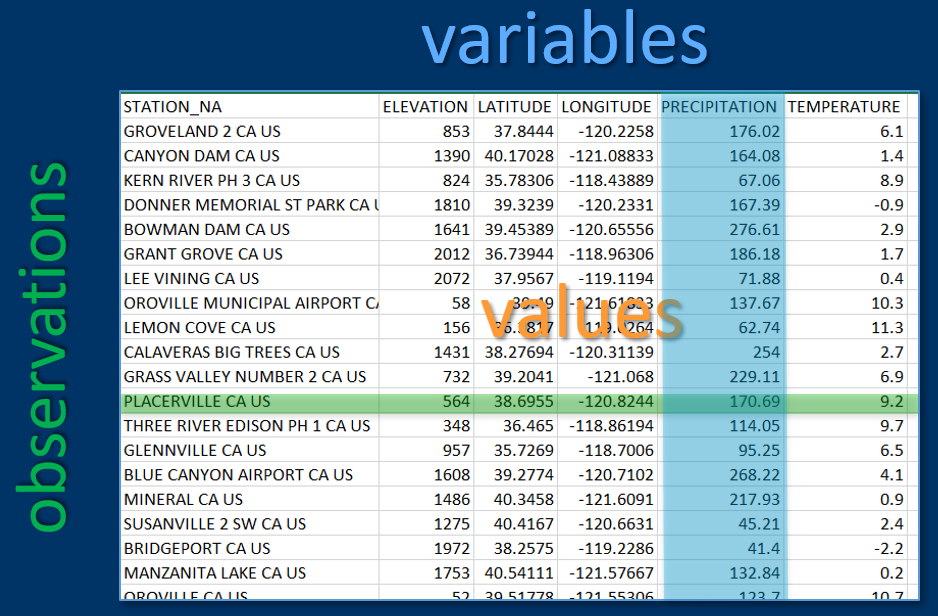
\includegraphics[width=0.75\linewidth]{img/variablesObservationsValues} 

}

\caption{Variables, observations, and values in rectangular data}\label{fig:introRectangular}
\end{figure}

\begin{Shaded}
\begin{Highlighting}[]
\FunctionTok{library}\NormalTok{(igisci)}
\NormalTok{sierraFeb}
\end{Highlighting}
\end{Shaded}

\begin{verbatim}
## # A tibble: 82 x 7
##    STATION_NAME    COUNTY ELEVATION LATITUDE LONGITUDE PRECIPITATION TEMPERATURE
##    <chr>           <chr>      <dbl>    <dbl>     <dbl>         <dbl>       <dbl>
##  1 GROVELAND 2, C~ Tuolu~     853.      37.8     -120.         176.          6.1
##  2 CANYON DAM, CA~ Plumas    1390.      40.2     -121.         164.          1.4
##  3 KERN RIVER PH ~ Kern       824.      35.8     -118.          67.1         8.9
##  4 DONNER MEMORIA~ Nevada    1810.      39.3     -120.         167.         -0.9
##  5 BOWMAN DAM, CA~ Nevada    1641.      39.5     -121.         277.          2.9
##  6 BRUSH CREEK RA~ Butte     1085.      39.7     -121.         296.         NA  
##  7 GRANT GROVE, C~ Tulare    2012.      36.7     -119.         186.          1.7
##  8 LEE VINING, CA~ Mono      2072.      38.0     -119.          71.9         0.4
##  9 OROVILLE MUNIC~ Butte       57.9     39.5     -122.         138.         10.3
## 10 LEMON COVE, CA~ Tulare     156.      36.4     -119.          62.7        11.3
## # i 72 more rows
\end{verbatim}

\section{Data Structures in R}\label{data-structures-in-r}

We've already started using the most common data structures -- scalars and vectors -- but haven't really talked about vectors yet, so we'll start there.

\subsection{Vectors}\label{vector}

A \index{vector}vector is an ordered collection of numbers, strings, vectors, data frames, etc. What we mostly refer to simply as vectors are formally called \index{atomic vectors}\textbf{atomic vectors}, which require that they be \emph{homogeneous} sets of whatever type we're referring to, such as a vector of numbers, a vector of strings, or a vector of dates/times.

You can create a simple vector with the \index{c()}\texttt{c()} function:

\begin{Shaded}
\begin{Highlighting}[]
\NormalTok{lats }\OtherTok{\textless{}{-}} \FunctionTok{c}\NormalTok{(}\FloatTok{37.5}\NormalTok{,}\FloatTok{47.4}\NormalTok{,}\FloatTok{29.4}\NormalTok{,}\FloatTok{33.4}\NormalTok{)}
\NormalTok{lats}
\end{Highlighting}
\end{Shaded}

\begin{verbatim}
## [1] 37.5 47.4 29.4 33.4
\end{verbatim}

\begin{Shaded}
\begin{Highlighting}[]
\NormalTok{states }\OtherTok{\textless{}{-}} \FunctionTok{c}\NormalTok{(}\StringTok{"VA"}\NormalTok{, }\StringTok{"WA"}\NormalTok{, }\StringTok{"TX"}\NormalTok{, }\StringTok{"AZ"}\NormalTok{)}
\NormalTok{states}
\end{Highlighting}
\end{Shaded}

\begin{verbatim}
## [1] "VA" "WA" "TX" "AZ"
\end{verbatim}

\begin{Shaded}
\begin{Highlighting}[]
\NormalTok{zips }\OtherTok{\textless{}{-}} \FunctionTok{c}\NormalTok{(}\DecValTok{23173}\NormalTok{, }\DecValTok{98801}\NormalTok{, }\DecValTok{78006}\NormalTok{, }\DecValTok{85001}\NormalTok{)}
\NormalTok{zips}
\end{Highlighting}
\end{Shaded}

\begin{verbatim}
## [1] 23173 98801 78006 85001
\end{verbatim}

The \index{class of a vector}class of a vector is the type of data it holds

\begin{Shaded}
\begin{Highlighting}[]
\NormalTok{tC }\OtherTok{\textless{}{-}} \FunctionTok{c}\NormalTok{(}\FloatTok{10.7}\NormalTok{, }\FloatTok{9.7}\NormalTok{, }\FloatTok{7.7}\NormalTok{, }\FloatTok{9.2}\NormalTok{, }\FloatTok{7.3}\NormalTok{, }\FloatTok{6.7}\NormalTok{)}
\FunctionTok{class}\NormalTok{(tC)}
\end{Highlighting}
\end{Shaded}

\begin{verbatim}
## [1] "numeric"
\end{verbatim}

Let's also introduce the handy \index{str}\texttt{str()} function, which in one step gives you a view of the class of an item and its content -- so its structure. We'll often use it in this book when we want to tell the reader what a data object contains, instead of listing a vector and its class separately, so instead of \ldots{}

\begin{Shaded}
\begin{Highlighting}[]
\NormalTok{tC}
\end{Highlighting}
\end{Shaded}

\begin{verbatim}
## [1] 10.7  9.7  7.7  9.2  7.3  6.7
\end{verbatim}

\begin{Shaded}
\begin{Highlighting}[]
\FunctionTok{class}\NormalTok{(tC)}
\end{Highlighting}
\end{Shaded}

\begin{verbatim}
## [1] "numeric"
\end{verbatim}

\ldots{} we'll just use \texttt{str()}:

\begin{Shaded}
\begin{Highlighting}[]
\FunctionTok{str}\NormalTok{(tC)}
\end{Highlighting}
\end{Shaded}

\begin{verbatim}
##  num [1:6] 10.7 9.7 7.7 9.2 7.3 6.7
\end{verbatim}

Vectors can only have one data class, and if mixed with character types, numeric elements will become character:

\begin{Shaded}
\begin{Highlighting}[]
\NormalTok{mixed }\OtherTok{\textless{}{-}} \FunctionTok{c}\NormalTok{(}\DecValTok{1}\NormalTok{, }\StringTok{"fred"}\NormalTok{, }\DecValTok{7}\NormalTok{)}
\FunctionTok{str}\NormalTok{(mixed)}
\end{Highlighting}
\end{Shaded}

\begin{verbatim}
##  chr [1:3] "1" "fred" "7"
\end{verbatim}

\begin{Shaded}
\begin{Highlighting}[]
\NormalTok{mixed[}\DecValTok{3}\NormalTok{]   }\CommentTok{\# gets a subset, example of coercion}
\end{Highlighting}
\end{Shaded}

\begin{verbatim}
## [1] "7"
\end{verbatim}

\subsubsection{NA}\label{NA}

\index{NA}Data science requires dealing with missing data by storing some sort of null value, called various things:

\begin{itemize}
\tightlist
\item
  null
\item
  nodata
\item
  \texttt{NA} ``not available'' or ``not applicable''
\end{itemize}

\begin{Shaded}
\begin{Highlighting}[]
\FunctionTok{as.numeric}\NormalTok{(}\FunctionTok{c}\NormalTok{(}\StringTok{"1"}\NormalTok{,}\StringTok{"Fred"}\NormalTok{,}\StringTok{"5"}\NormalTok{)) }\CommentTok{\# note NA introduced by coercion}
\end{Highlighting}
\end{Shaded}

\begin{verbatim}
## [1]  1 NA  5
\end{verbatim}

Note that \texttt{NA} doesn't really have a data class. The above example created a numeric vector with the one it couldn't figure out being assigned \texttt{NA}. \emph{Remember that vectors (and matrices and arrays) have to be all the same data class.} A character vector can also include \texttt{NA}s. Both of the following are valid vectors, with the second item being \texttt{NA}:

\begin{Shaded}
\begin{Highlighting}[]
\FunctionTok{c}\NormalTok{(}\DecValTok{5}\NormalTok{,}\ConstantTok{NA}\NormalTok{,}\DecValTok{7}\NormalTok{)}
\FunctionTok{c}\NormalTok{(}\StringTok{"alpha"}\NormalTok{,}\ConstantTok{NA}\NormalTok{,}\StringTok{"delta"}\NormalTok{)}
\end{Highlighting}
\end{Shaded}

\begin{verbatim}
## [1]  5 NA  7
## [1] "alpha" NA      "delta"
\end{verbatim}

\begin{quote}
Note that we typed \texttt{NA} without quotations. It's kind of like a special constant, like the \texttt{TRUE} and \texttt{FALSE} logical values, neither of which uses quotations.
\end{quote}

We often want to ignore \texttt{NA} in statistical summaries. Where normally the summary statistic can only return \texttt{NA}\ldots{}

\begin{Shaded}
\begin{Highlighting}[]
\FunctionTok{mean}\NormalTok{(}\FunctionTok{as.numeric}\NormalTok{(}\FunctionTok{c}\NormalTok{(}\StringTok{"1"}\NormalTok{, }\StringTok{"Fred"}\NormalTok{, }\StringTok{"5"}\NormalTok{)))}
\end{Highlighting}
\end{Shaded}

\begin{verbatim}
## [1] NA
\end{verbatim}

\ldots{} with \texttt{na.rm=T} you can still get the result for all actual data:

\begin{Shaded}
\begin{Highlighting}[]
\FunctionTok{mean}\NormalTok{(}\FunctionTok{as.numeric}\NormalTok{(}\FunctionTok{c}\NormalTok{(}\StringTok{"1"}\NormalTok{, }\StringTok{"Fred"}\NormalTok{, }\StringTok{"5"}\NormalTok{)), }\AttributeTok{na.rm=}\NormalTok{T)}
\end{Highlighting}
\end{Shaded}

\begin{verbatim}
## [1] 3
\end{verbatim}

Don't confuse with \index{nan}\texttt{nan} (``not a number''), which is used for things like imaginary numbers (explore the help for more on this), as you can see here:

\begin{Shaded}
\begin{Highlighting}[]
\FunctionTok{is.nan}\NormalTok{(}\ConstantTok{NA}\NormalTok{)}
\end{Highlighting}
\end{Shaded}

\begin{verbatim}
## [1] FALSE
\end{verbatim}

\begin{Shaded}
\begin{Highlighting}[]
\FunctionTok{is.na}\NormalTok{(}\FunctionTok{as.numeric}\NormalTok{(}\StringTok{\textquotesingle{}\textquotesingle{}}\NormalTok{))}
\end{Highlighting}
\end{Shaded}

\begin{verbatim}
## [1] TRUE
\end{verbatim}

\begin{Shaded}
\begin{Highlighting}[]
\FunctionTok{is.nan}\NormalTok{(}\FunctionTok{as.numeric}\NormalTok{(}\StringTok{\textquotesingle{}\textquotesingle{}}\NormalTok{))}
\end{Highlighting}
\end{Shaded}

\begin{verbatim}
## [1] FALSE
\end{verbatim}

\begin{Shaded}
\begin{Highlighting}[]
\NormalTok{i }\OtherTok{\textless{}{-}} \FunctionTok{sqrt}\NormalTok{(}\SpecialCharTok{{-}}\DecValTok{1}\NormalTok{)}
\FunctionTok{is.na}\NormalTok{(i) }\CommentTok{\# interestingly nan is also na}
\end{Highlighting}
\end{Shaded}

\begin{verbatim}
## [1] TRUE
\end{verbatim}

\begin{Shaded}
\begin{Highlighting}[]
\FunctionTok{is.nan}\NormalTok{(i)}
\end{Highlighting}
\end{Shaded}

\begin{verbatim}
## [1] TRUE
\end{verbatim}

\subsubsection{Creating a vector from a sequence}\label{creating-a-vector-from-a-sequence}

We often need \index{sequences of values}sequences of values, and there are a few ways of creating them. The following three examples are equivalent:

\begin{verbatim}
seq(1,10)
1:10
c(1,2,3,4,5,6,7,8,9,10)
\end{verbatim}

The \index{seq}\texttt{seq()} function has special uses like using a step parameter:

\begin{Shaded}
\begin{Highlighting}[]
\FunctionTok{seq}\NormalTok{(}\DecValTok{2}\NormalTok{,}\DecValTok{10}\NormalTok{,}\DecValTok{2}\NormalTok{)}
\end{Highlighting}
\end{Shaded}

\begin{verbatim}
## [1]  2  4  6  8 10
\end{verbatim}

\subsubsection{Vectorization and vector arithmetic}\label{vectorization}

Arithmetic on vectors operates element-wise, a process called \index{vectorization}\emph{vectorization}.

\begin{Shaded}
\begin{Highlighting}[]
\NormalTok{elev }\OtherTok{\textless{}{-}} \FunctionTok{c}\NormalTok{(}\DecValTok{52}\NormalTok{,}\DecValTok{394}\NormalTok{,}\DecValTok{510}\NormalTok{,}\DecValTok{564}\NormalTok{,}\DecValTok{725}\NormalTok{,}\DecValTok{848}\NormalTok{,}\DecValTok{1042}\NormalTok{,}\DecValTok{1225}\NormalTok{,}\DecValTok{1486}\NormalTok{,}\DecValTok{1775}\NormalTok{,}\DecValTok{1899}\NormalTok{,}\DecValTok{2551}\NormalTok{)}
\NormalTok{elevft }\OtherTok{\textless{}{-}}\NormalTok{ elev }\SpecialCharTok{/} \FloatTok{0.3048}
\NormalTok{elevft}
\end{Highlighting}
\end{Shaded}

\begin{verbatim}
##  [1]  170.6037 1292.6509 1673.2283 1850.3937 2378.6089 2782.1522 3418.6352
##  [8] 4019.0289 4875.3281 5823.4908 6230.3150 8369.4226
\end{verbatim}

Another example, with two vectors:

\begin{Shaded}
\begin{Highlighting}[]
\NormalTok{temp03 }\OtherTok{\textless{}{-}} \FunctionTok{c}\NormalTok{(}\FloatTok{13.1}\NormalTok{,}\FloatTok{11.4}\NormalTok{,}\FloatTok{9.4}\NormalTok{,}\FloatTok{10.9}\NormalTok{,}\FloatTok{8.9}\NormalTok{,}\FloatTok{8.4}\NormalTok{,}\FloatTok{6.7}\NormalTok{,}\FloatTok{7.6}\NormalTok{,}\FloatTok{2.8}\NormalTok{,}\FloatTok{1.6}\NormalTok{,}\FloatTok{1.2}\NormalTok{,}\SpecialCharTok{{-}}\FloatTok{2.1}\NormalTok{)}
\NormalTok{temp02 }\OtherTok{\textless{}{-}} \FunctionTok{c}\NormalTok{(}\FloatTok{10.7}\NormalTok{,}\FloatTok{9.7}\NormalTok{,}\FloatTok{7.7}\NormalTok{,}\FloatTok{9.2}\NormalTok{,}\FloatTok{7.3}\NormalTok{,}\FloatTok{6.7}\NormalTok{,}\FloatTok{4.0}\NormalTok{,}\FloatTok{5.0}\NormalTok{,}\FloatTok{0.9}\NormalTok{,}\SpecialCharTok{{-}}\FloatTok{1.1}\NormalTok{,}\SpecialCharTok{{-}}\FloatTok{0.8}\NormalTok{,}\SpecialCharTok{{-}}\FloatTok{4.4}\NormalTok{)}
\NormalTok{tempdiff }\OtherTok{\textless{}{-}}\NormalTok{ temp03 }\SpecialCharTok{{-}}\NormalTok{ temp02}
\NormalTok{tempdiff}
\end{Highlighting}
\end{Shaded}

\begin{verbatim}
##  [1] 2.4 1.7 1.7 1.7 1.6 1.7 2.7 2.6 1.9 2.7 2.0 2.3
\end{verbatim}

\subsubsection{Plotting vectors}\label{plotting-vectors}

Vectors of Feb temperature, elevation, and latitude at stations in the Sierra:

\begin{Shaded}
\begin{Highlighting}[]
\NormalTok{tC }\OtherTok{\textless{}{-}} \FunctionTok{c}\NormalTok{(}\FloatTok{10.7}\NormalTok{,  }\FloatTok{9.7}\NormalTok{,  }\FloatTok{7.7}\NormalTok{,  }\FloatTok{9.2}\NormalTok{,  }\FloatTok{7.3}\NormalTok{,  }\FloatTok{6.7}\NormalTok{,  }\FloatTok{4.0}\NormalTok{,  }\FloatTok{5.0}\NormalTok{,  }\FloatTok{0.9}\NormalTok{, }\SpecialCharTok{{-}}\FloatTok{1.1}\NormalTok{, }\SpecialCharTok{{-}}\FloatTok{0.8}\NormalTok{,}\SpecialCharTok{{-}}\FloatTok{4.4}\NormalTok{)}
\NormalTok{elev }\OtherTok{\textless{}{-}}   \FunctionTok{c}\NormalTok{(}\DecValTok{52}\NormalTok{,  }\DecValTok{394}\NormalTok{,  }\DecValTok{510}\NormalTok{,  }\DecValTok{564}\NormalTok{,  }\DecValTok{725}\NormalTok{,  }\DecValTok{848}\NormalTok{, }\DecValTok{1042}\NormalTok{, }\DecValTok{1225}\NormalTok{, }\DecValTok{1486}\NormalTok{, }\DecValTok{1775}\NormalTok{, }\DecValTok{1899}\NormalTok{, }\DecValTok{2551}\NormalTok{)}
\NormalTok{lat }\OtherTok{\textless{}{-}} \FunctionTok{c}\NormalTok{(}\FloatTok{39.52}\NormalTok{,}\FloatTok{38.91}\NormalTok{,}\FloatTok{37.97}\NormalTok{,}\FloatTok{38.70}\NormalTok{,}\FloatTok{39.09}\NormalTok{,}\FloatTok{39.25}\NormalTok{,}\FloatTok{39.94}\NormalTok{,}\FloatTok{37.75}\NormalTok{,}\FloatTok{40.35}\NormalTok{,}\FloatTok{39.33}\NormalTok{,}\FloatTok{39.17}\NormalTok{,}\FloatTok{38.21}\NormalTok{)}
\end{Highlighting}
\end{Shaded}

\textbf{Plot individually by index vs a scatterplot}

\index{scatterplot}We'll use the \index{plot}\texttt{plot()} function to visualize what's in a vector. The \texttt{plot()} function will create an output based upon its best guess of what you're wanting to see, and will depend on the nature of the data you provide it. We'll be looking at a lot of ways to visualize data soon, but it's often useful to just see what \texttt{plot()} gives you. In this case, it just makes a bivariate plot where the x dimension is the sequential index of the vector from 1 through the length of the vector, and the values are in the y dimension. For comparison is a scatterplot with \texttt{elevation} on the x axis (Figure \ref{fig:twoplots}).

\begin{Shaded}
\begin{Highlighting}[]
\FunctionTok{plot}\NormalTok{(tC)}
\FunctionTok{plot}\NormalTok{(elev,tC)}
\end{Highlighting}
\end{Shaded}

\begin{figure}

{\centering 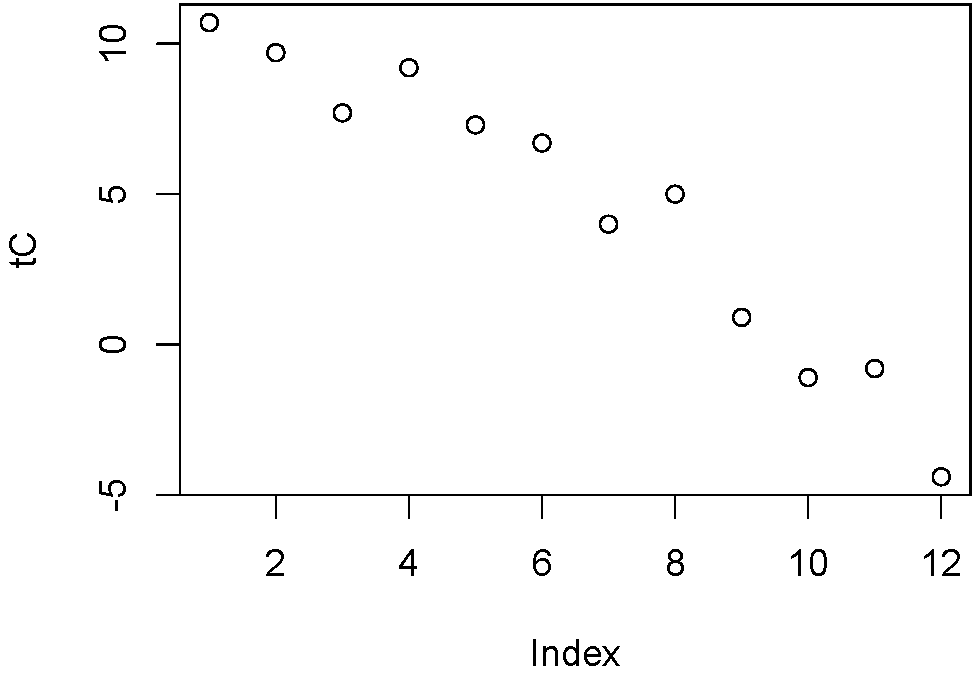
\includegraphics[width=0.5\linewidth]{EnvDataScience_files/figure-latex/twoplots-1} 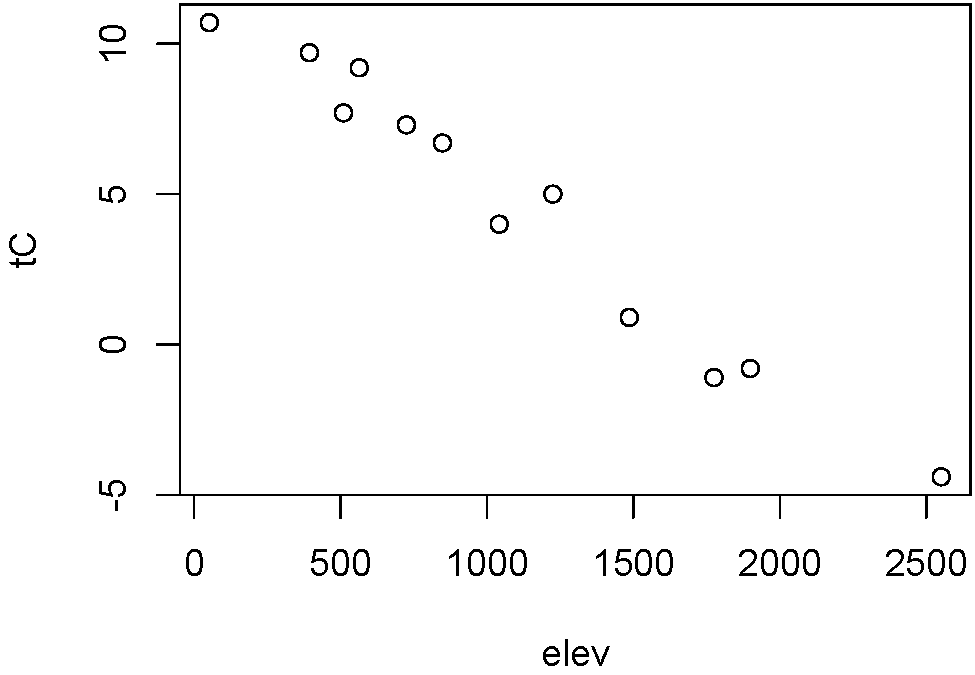
\includegraphics[width=0.5\linewidth]{EnvDataScience_files/figure-latex/twoplots-2} 

}

\caption{Temperature plotted by index (left) and elevation (right)}\label{fig:twoplots}
\end{figure}

\subsubsection{Named indices}\label{named-indices}

\index{named indices}Vectors themselves have names (like \texttt{elev}, \texttt{tC}, and \texttt{lat} above), but individual indices can also be named.

\begin{Shaded}
\begin{Highlighting}[]
\NormalTok{fips }\OtherTok{\textless{}{-}} \FunctionTok{c}\NormalTok{(}\DecValTok{16}\NormalTok{, }\DecValTok{30}\NormalTok{, }\DecValTok{56}\NormalTok{)}
\FunctionTok{str}\NormalTok{(fips)}
\end{Highlighting}
\end{Shaded}

\begin{verbatim}
##  num [1:3] 16 30 56
\end{verbatim}

\begin{Shaded}
\begin{Highlighting}[]
\NormalTok{fips }\OtherTok{\textless{}{-}} \FunctionTok{c}\NormalTok{(}\AttributeTok{idaho =} \DecValTok{16}\NormalTok{, }\AttributeTok{montana =} \DecValTok{30}\NormalTok{, }\AttributeTok{wyoming =} \DecValTok{56}\NormalTok{)}
\FunctionTok{str}\NormalTok{(fips)}
\end{Highlighting}
\end{Shaded}

\begin{verbatim}
##  Named num [1:3] 16 30 56
##  - attr(*, "names")= chr [1:3] "idaho" "montana" "wyoming"
\end{verbatim}

The reason we might do this is so you can refer to observations by name instead of index, maybe to filter observations based on criteria where the name will be useful. The following are equivalent:

\begin{Shaded}
\begin{Highlighting}[]
\NormalTok{fips[}\DecValTok{2}\NormalTok{]}
\end{Highlighting}
\end{Shaded}

\begin{verbatim}
## montana 
##      30
\end{verbatim}

\begin{Shaded}
\begin{Highlighting}[]
\NormalTok{fips[}\StringTok{"montana"}\NormalTok{]}
\end{Highlighting}
\end{Shaded}

\begin{verbatim}
## montana 
##      30
\end{verbatim}

The \index{names}\texttt{names()} function can be used to display a character vector of names, or assign names from a character vector:

\begin{Shaded}
\begin{Highlighting}[]
\FunctionTok{names}\NormalTok{(fips) }\CommentTok{\# returns a character vector of names}
\end{Highlighting}
\end{Shaded}

\begin{verbatim}
## [1] "idaho"   "montana" "wyoming"
\end{verbatim}

\begin{Shaded}
\begin{Highlighting}[]
\FunctionTok{names}\NormalTok{(fips) }\OtherTok{\textless{}{-}} \FunctionTok{c}\NormalTok{(}\StringTok{"Idaho"}\NormalTok{,}\StringTok{"Montana"}\NormalTok{,}\StringTok{"Wyoming"}\NormalTok{)}
\FunctionTok{names}\NormalTok{(fips)}
\end{Highlighting}
\end{Shaded}

\begin{verbatim}
## [1] "Idaho"   "Montana" "Wyoming"
\end{verbatim}

\subsubsection{Length of a vector}\label{length-of-a-vector}

One thing that we often need to know is just how many items are in our vector, which we can get with the \texttt{length()} function.

\begin{Shaded}
\begin{Highlighting}[]
\FunctionTok{length}\NormalTok{(fips)}
\end{Highlighting}
\end{Shaded}

\begin{verbatim}
## [1] 3
\end{verbatim}

\begin{Shaded}
\begin{Highlighting}[]
\FunctionTok{length}\NormalTok{(}\FunctionTok{seq}\NormalTok{(}\DecValTok{2}\NormalTok{,}\DecValTok{10}\NormalTok{,}\DecValTok{2}\NormalTok{))}
\end{Highlighting}
\end{Shaded}

\begin{verbatim}
## [1] 5
\end{verbatim}

\begin{quote}
This will also apply to other types of objects, but is easily understood with vectors.
\end{quote}

\subsection{Lists}\label{list}

\index{lists}Lists can be heterogeneous, with multiple class types. Lists are actually used a lot in R, and are created by many operations, but they can be confusing to get used to especially when it's unclear what we'll be using them for. We'll avoid them for a while, and look into specific examples as we need them.

\subsection{Matrices}\label{matrix}

\index{matrices}Vectors are commonly used as a column in a matrix (or as we'll see, a data frame), like a variable

\begin{Shaded}
\begin{Highlighting}[]
\NormalTok{tC }\OtherTok{\textless{}{-}} \FunctionTok{c}\NormalTok{(}\FloatTok{10.7}\NormalTok{,  }\FloatTok{9.7}\NormalTok{,  }\FloatTok{7.7}\NormalTok{,  }\FloatTok{9.2}\NormalTok{,  }\FloatTok{7.3}\NormalTok{,  }\FloatTok{6.7}\NormalTok{,  }\FloatTok{4.0}\NormalTok{,  }\FloatTok{5.0}\NormalTok{,  }\FloatTok{0.9}\NormalTok{, }\SpecialCharTok{{-}}\FloatTok{1.1}\NormalTok{, }\SpecialCharTok{{-}}\FloatTok{0.8}\NormalTok{,}\SpecialCharTok{{-}}\FloatTok{4.4}\NormalTok{)}
\NormalTok{elev }\OtherTok{\textless{}{-}}   \FunctionTok{c}\NormalTok{(}\DecValTok{52}\NormalTok{,  }\DecValTok{394}\NormalTok{,  }\DecValTok{510}\NormalTok{,  }\DecValTok{564}\NormalTok{,  }\DecValTok{725}\NormalTok{,  }\DecValTok{848}\NormalTok{, }\DecValTok{1042}\NormalTok{, }\DecValTok{1225}\NormalTok{, }\DecValTok{1486}\NormalTok{, }\DecValTok{1775}\NormalTok{, }\DecValTok{1899}\NormalTok{, }\DecValTok{2551}\NormalTok{)}
\NormalTok{lat }\OtherTok{\textless{}{-}} \FunctionTok{c}\NormalTok{(}\FloatTok{39.52}\NormalTok{,}\FloatTok{38.91}\NormalTok{,}\FloatTok{37.97}\NormalTok{,}\FloatTok{38.70}\NormalTok{,}\FloatTok{39.09}\NormalTok{,}\FloatTok{39.25}\NormalTok{,}\FloatTok{39.94}\NormalTok{,}\FloatTok{37.75}\NormalTok{,}\FloatTok{40.35}\NormalTok{,}\FloatTok{39.33}\NormalTok{,}\FloatTok{39.17}\NormalTok{,}\FloatTok{38.21}\NormalTok{)}
\end{Highlighting}
\end{Shaded}

\textbf{Building a matrix from vectors as columns}

The \texttt{cbind()} in base R binds multiple vectors into columns in a matrix.

\begin{Shaded}
\begin{Highlighting}[]
\NormalTok{sierradata }\OtherTok{\textless{}{-}} \FunctionTok{cbind}\NormalTok{(tC, elev, lat)}
\FunctionTok{class}\NormalTok{(sierradata)}
\end{Highlighting}
\end{Shaded}

\begin{verbatim}
## [1] "matrix" "array"
\end{verbatim}

\begin{Shaded}
\begin{Highlighting}[]
\FunctionTok{str}\NormalTok{(sierradata)}
\end{Highlighting}
\end{Shaded}

\begin{verbatim}
##  num [1:12, 1:3] 10.7 9.7 7.7 9.2 7.3 6.7 4 5 0.9 -1.1 ...
##  - attr(*, "dimnames")=List of 2
##   ..$ : NULL
##   ..$ : chr [1:3] "tC" "elev" "lat"
\end{verbatim}

\begin{Shaded}
\begin{Highlighting}[]
\NormalTok{sierradata}
\end{Highlighting}
\end{Shaded}

\begin{verbatim}
##         tC elev   lat
##  [1,] 10.7   52 39.52
##  [2,]  9.7  394 38.91
##  [3,]  7.7  510 37.97
##  [4,]  9.2  564 38.70
##  [5,]  7.3  725 39.09
##  [6,]  6.7  848 39.25
##  [7,]  4.0 1042 39.94
##  [8,]  5.0 1225 37.75
##  [9,]  0.9 1486 40.35
## [10,] -1.1 1775 39.33
## [11,] -0.8 1899 39.17
## [12,] -4.4 2551 38.21
\end{verbatim}

\begin{quote}
Remember that matrices are similar to (atomic) vectors in that they all have to be of the same data type.
\end{quote}

\subsubsection{Dimensions for arrays and matrices}\label{dimensions-for-arrays-and-matrices}

\index{dimensions for arrays and matrices}Note: a matrix is just a 2D array. Arrays have 1, 3, or more \index{dim}dimensions.

\begin{Shaded}
\begin{Highlighting}[]
\FunctionTok{dim}\NormalTok{(sierradata)}
\end{Highlighting}
\end{Shaded}

\begin{verbatim}
## [1] 12  3
\end{verbatim}

It's also important to remember that a matrix or an array is a vector with dimensions, and we can change those dimensions in various ways as long as they work for the length of the vector.

\begin{Shaded}
\begin{Highlighting}[]
\NormalTok{a }\OtherTok{\textless{}{-}} \DecValTok{1}\SpecialCharTok{:}\DecValTok{12}
\FunctionTok{dim}\NormalTok{(a) }\OtherTok{\textless{}{-}} \FunctionTok{c}\NormalTok{(}\DecValTok{3}\NormalTok{, }\DecValTok{4}\NormalTok{)   }\CommentTok{\# matrix}
\FunctionTok{class}\NormalTok{(a)}
\end{Highlighting}
\end{Shaded}

\begin{verbatim}
## [1] "matrix" "array"
\end{verbatim}

\begin{Shaded}
\begin{Highlighting}[]
\FunctionTok{dim}\NormalTok{(a) }\OtherTok{\textless{}{-}} \FunctionTok{c}\NormalTok{(}\DecValTok{2}\NormalTok{,}\DecValTok{3}\NormalTok{,}\DecValTok{2}\NormalTok{)  }\CommentTok{\# 3D array}
\FunctionTok{class}\NormalTok{(a)}
\end{Highlighting}
\end{Shaded}

\begin{verbatim}
## [1] "array"
\end{verbatim}

\begin{Shaded}
\begin{Highlighting}[]
\FunctionTok{dim}\NormalTok{(a) }\OtherTok{\textless{}{-}} \DecValTok{12}        \CommentTok{\# 1D array}
\FunctionTok{class}\NormalTok{(a)}
\end{Highlighting}
\end{Shaded}

\begin{verbatim}
## [1] "array"
\end{verbatim}

\begin{Shaded}
\begin{Highlighting}[]
\NormalTok{b }\OtherTok{\textless{}{-}} \FunctionTok{matrix}\NormalTok{(}\DecValTok{1}\SpecialCharTok{:}\DecValTok{12}\NormalTok{, }\AttributeTok{ncol=}\DecValTok{1}\NormalTok{)  }\CommentTok{\# 1 column matrix is allowed}
\end{Highlighting}
\end{Shaded}

We just saw that we can change the dimensions of an existing matrix or array. But what if the matrix has names for its columns? I wasn't sure so following my basic philosophy of \index{empirical programming}\emph{empirical programming} I just tried it:

\begin{Shaded}
\begin{Highlighting}[]
\FunctionTok{dim}\NormalTok{(sierradata) }\OtherTok{\textless{}{-}} \FunctionTok{c}\NormalTok{(}\DecValTok{3}\NormalTok{,}\DecValTok{12}\NormalTok{)}
\NormalTok{sierradata}
\end{Highlighting}
\end{Shaded}

\begin{verbatim}
##      [,1] [,2] [,3] [,4] [,5] [,6] [,7] [,8]  [,9] [,10] [,11] [,12]
## [1,] 10.7  9.2  4.0 -1.1   52  564 1042 1775 39.52 38.70 39.94 39.33
## [2,]  9.7  7.3  5.0 -0.8  394  725 1225 1899 38.91 39.09 37.75 39.17
## [3,]  7.7  6.7  0.9 -4.4  510  848 1486 2551 37.97 39.25 40.35 38.21
\end{verbatim}

So the answer is that it gets rid of the column names, and we can also see that redimensioning changes a lot more about how the data appears (though \texttt{dim(sierradata)\ \textless{}-\ c(12,3)} will return it to its original structure, but without column names). It's actually a little odd that matrices can have column names, because that really just makes them seem like data frames, so let's look at those next. Let's consider a situation where we want to create a rectangular data set from some data for a set of states:

\begin{Shaded}
\begin{Highlighting}[]
\NormalTok{abb }\OtherTok{\textless{}{-}} \FunctionTok{c}\NormalTok{(}\StringTok{"CO"}\NormalTok{,}\StringTok{"WY"}\NormalTok{,}\StringTok{"UT"}\NormalTok{)}
\NormalTok{area }\OtherTok{\textless{}{-}} \FunctionTok{c}\NormalTok{(}\DecValTok{269837}\NormalTok{, }\DecValTok{253600}\NormalTok{, }\DecValTok{84899}\NormalTok{)}
\NormalTok{pop }\OtherTok{\textless{}{-}} \FunctionTok{c}\NormalTok{(}\DecValTok{5758736}\NormalTok{, }\DecValTok{578759}\NormalTok{, }\DecValTok{3205958}\NormalTok{)}
\end{Highlighting}
\end{Shaded}

We can use \index{cbind}\texttt{cbind} to create a matrix out of them, just like we did with the \texttt{sierradata} above

\begin{Shaded}
\begin{Highlighting}[]
\FunctionTok{cbind}\NormalTok{(abb,area,pop)}
\end{Highlighting}
\end{Shaded}

\begin{verbatim}
##      abb  area     pop      
## [1,] "CO" "269837" "5758736"
## [2,] "WY" "253600" "578759" 
## [3,] "UT" "84899"  "3205958"
\end{verbatim}

But notice what it did -- area and pop were converted to character type. This reminds us that \emph{matrices are still atomic vectors -- all of the same class}. So to comply with this, the numbers were converted to character strings, since you can't convert character strings to numbers.

This isn't very satisfactory as a data object, so we'll need to use a data frame, which is \emph{not} a vector, though its individual column variables are vectors.

\subsubsection{Length of a matrix?}\label{length-of-a-matrix}

A matrix is still a vector, so its length is the length of the overall vector.

\begin{Shaded}
\begin{Highlighting}[]
\NormalTok{a }\OtherTok{\textless{}{-}} \DecValTok{1}\SpecialCharTok{:}\DecValTok{12}
\FunctionTok{dim}\NormalTok{(a) }\OtherTok{\textless{}{-}} \FunctionTok{c}\NormalTok{(}\DecValTok{3}\NormalTok{, }\DecValTok{4}\NormalTok{)   }\CommentTok{\# matrix}
\NormalTok{a}
\end{Highlighting}
\end{Shaded}

\begin{verbatim}
##      [,1] [,2] [,3] [,4]
## [1,]    1    4    7   10
## [2,]    2    5    8   11
## [3,]    3    6    9   12
\end{verbatim}

\begin{Shaded}
\begin{Highlighting}[]
\FunctionTok{length}\NormalTok{(a)}
\end{Highlighting}
\end{Shaded}

\begin{verbatim}
## [1] 12
\end{verbatim}

\subsection{Data frames}\label{dataframes}

A \index{data frame}data frame is a database with variables in columns and rows of observations. They're kind of like a spreadsheet with rules (like the first row is field names) or a matrix that can have variables of unique types. Data frames will be very important for data analysis and GIS. We can easily create a data frame using the \texttt{data.frame} function, and then display it simply\ldots{}

\begin{Shaded}
\begin{Highlighting}[]
\NormalTok{threeStates }\OtherTok{\textless{}{-}} \FunctionTok{data.frame}\NormalTok{(}\FunctionTok{cbind}\NormalTok{(abb,area,pop))}
\NormalTok{threeStates}
\end{Highlighting}
\end{Shaded}

\begin{verbatim}
##   abb   area     pop
## 1  CO 269837 5758736
## 2  WY 253600  578759
## 3  UT  84899 3205958
\end{verbatim}

\ldots{} or use one of several table display tools. For instance, the \texttt{gt} tool in the \texttt{gt} package is designed for creating tables for a report, with many options to optimize its design for a given purpose. Typically you'd use it for the final results, as a static table with everything shown at once. See \url{https://gt.rstudio.com/} for more information.

\begin{Shaded}
\begin{Highlighting}[]
\NormalTok{gt}\SpecialCharTok{::}\FunctionTok{gt}\NormalTok{(threeStates)}
\end{Highlighting}
\end{Shaded}

\begin{table}[t]
\fontsize{12.0pt}{14.0pt}\selectfont
\begin{tabular*}{\linewidth}{@{\extracolsep{\fill}}lrr}
\toprule
abb & area & pop \\ 
\midrule\addlinespace[2.5pt]
CO & 269837 & 5758736 \\ 
WY & 253600 & 578759 \\ 
UT & 84899 & 3205958 \\ 
\bottomrule
\end{tabular*}
\end{table}

Before we get started looking further into data frames, we're going to use the \index{palmerpenguins}\texttt{palmerpenguins} data set, so you need to install it if you haven't yet, and then load the library with:

\begin{Shaded}
\begin{Highlighting}[]
\FunctionTok{library}\NormalTok{(palmerpenguins)}
\end{Highlighting}
\end{Shaded}

I'd encourage you to learn more about this dataset at \url{https://allisonhorst.github.io/palmerpenguins/articles/intro.html}(Horst et al. (\citeproc{ref-palmer}{2020})) (Figures \ref{fig:introPenguins} and \ref{fig:introPenguinMorphometry}). It will be useful for a variety of demonstrations using numerical morphometric variables as well as a couple of categorical factors (species and island).

\begin{figure}

{\centering 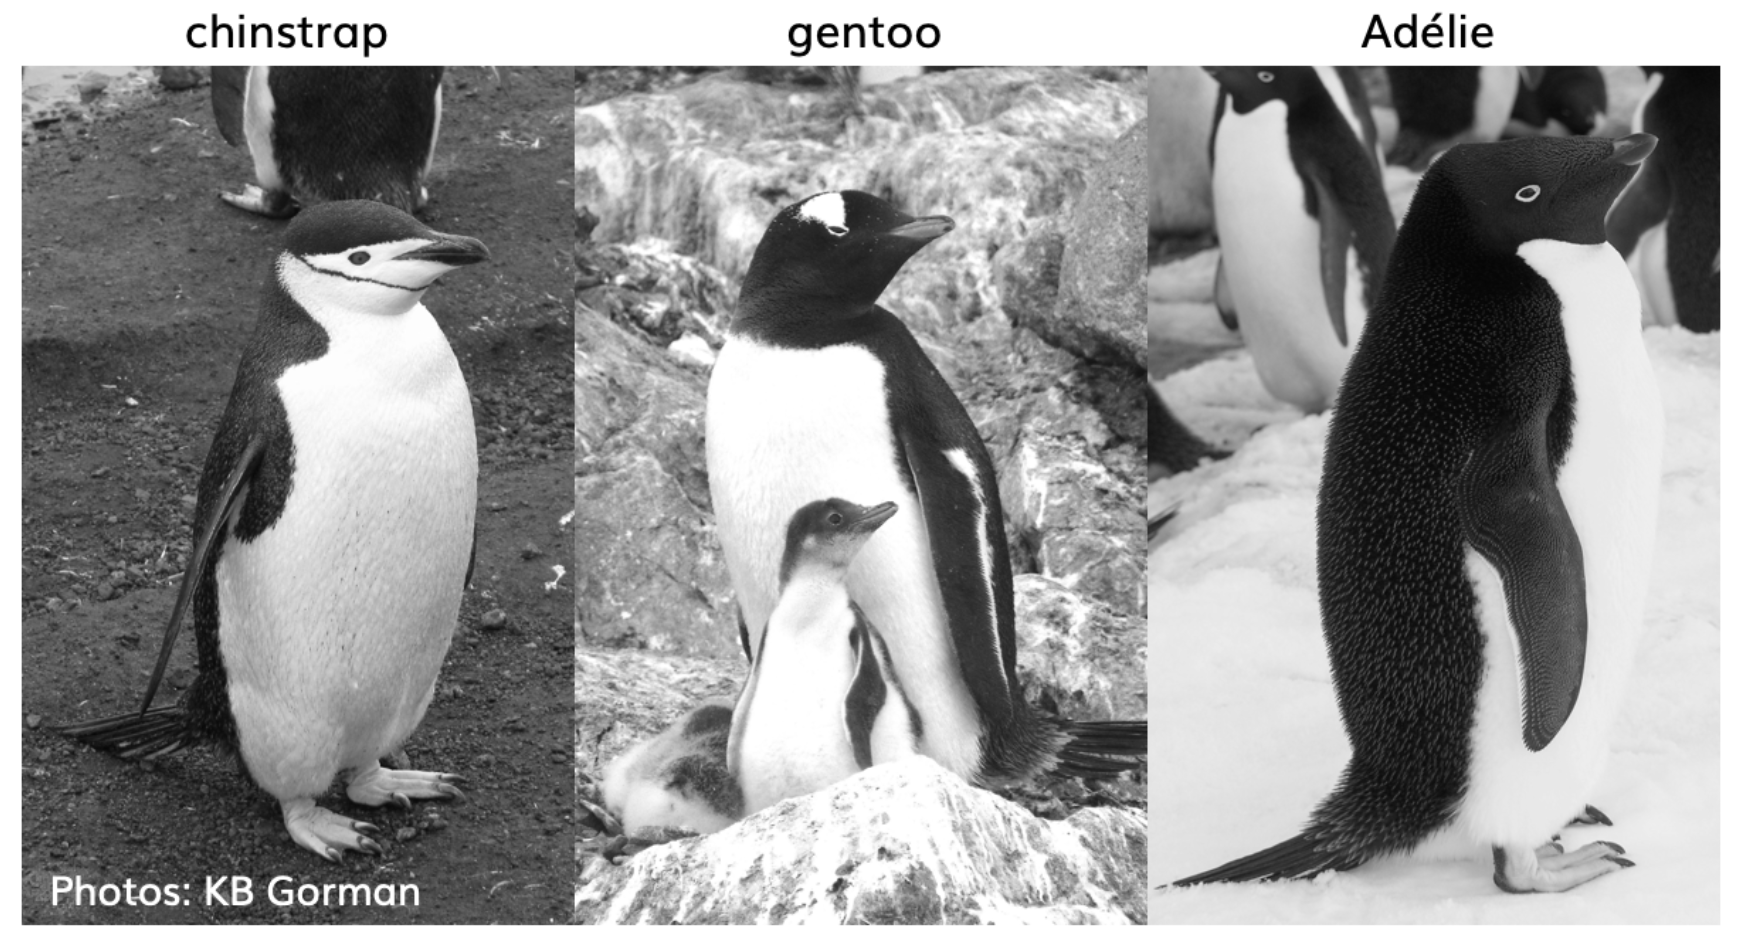
\includegraphics[width=0.75\linewidth]{img/PalmerPenguinsCrop} 

}

\caption{The three penguin species in palmerpenguins. Photos by KB Gorman. Used with permission}\label{fig:introPenguins}
\end{figure}

\begin{figure}

{\centering 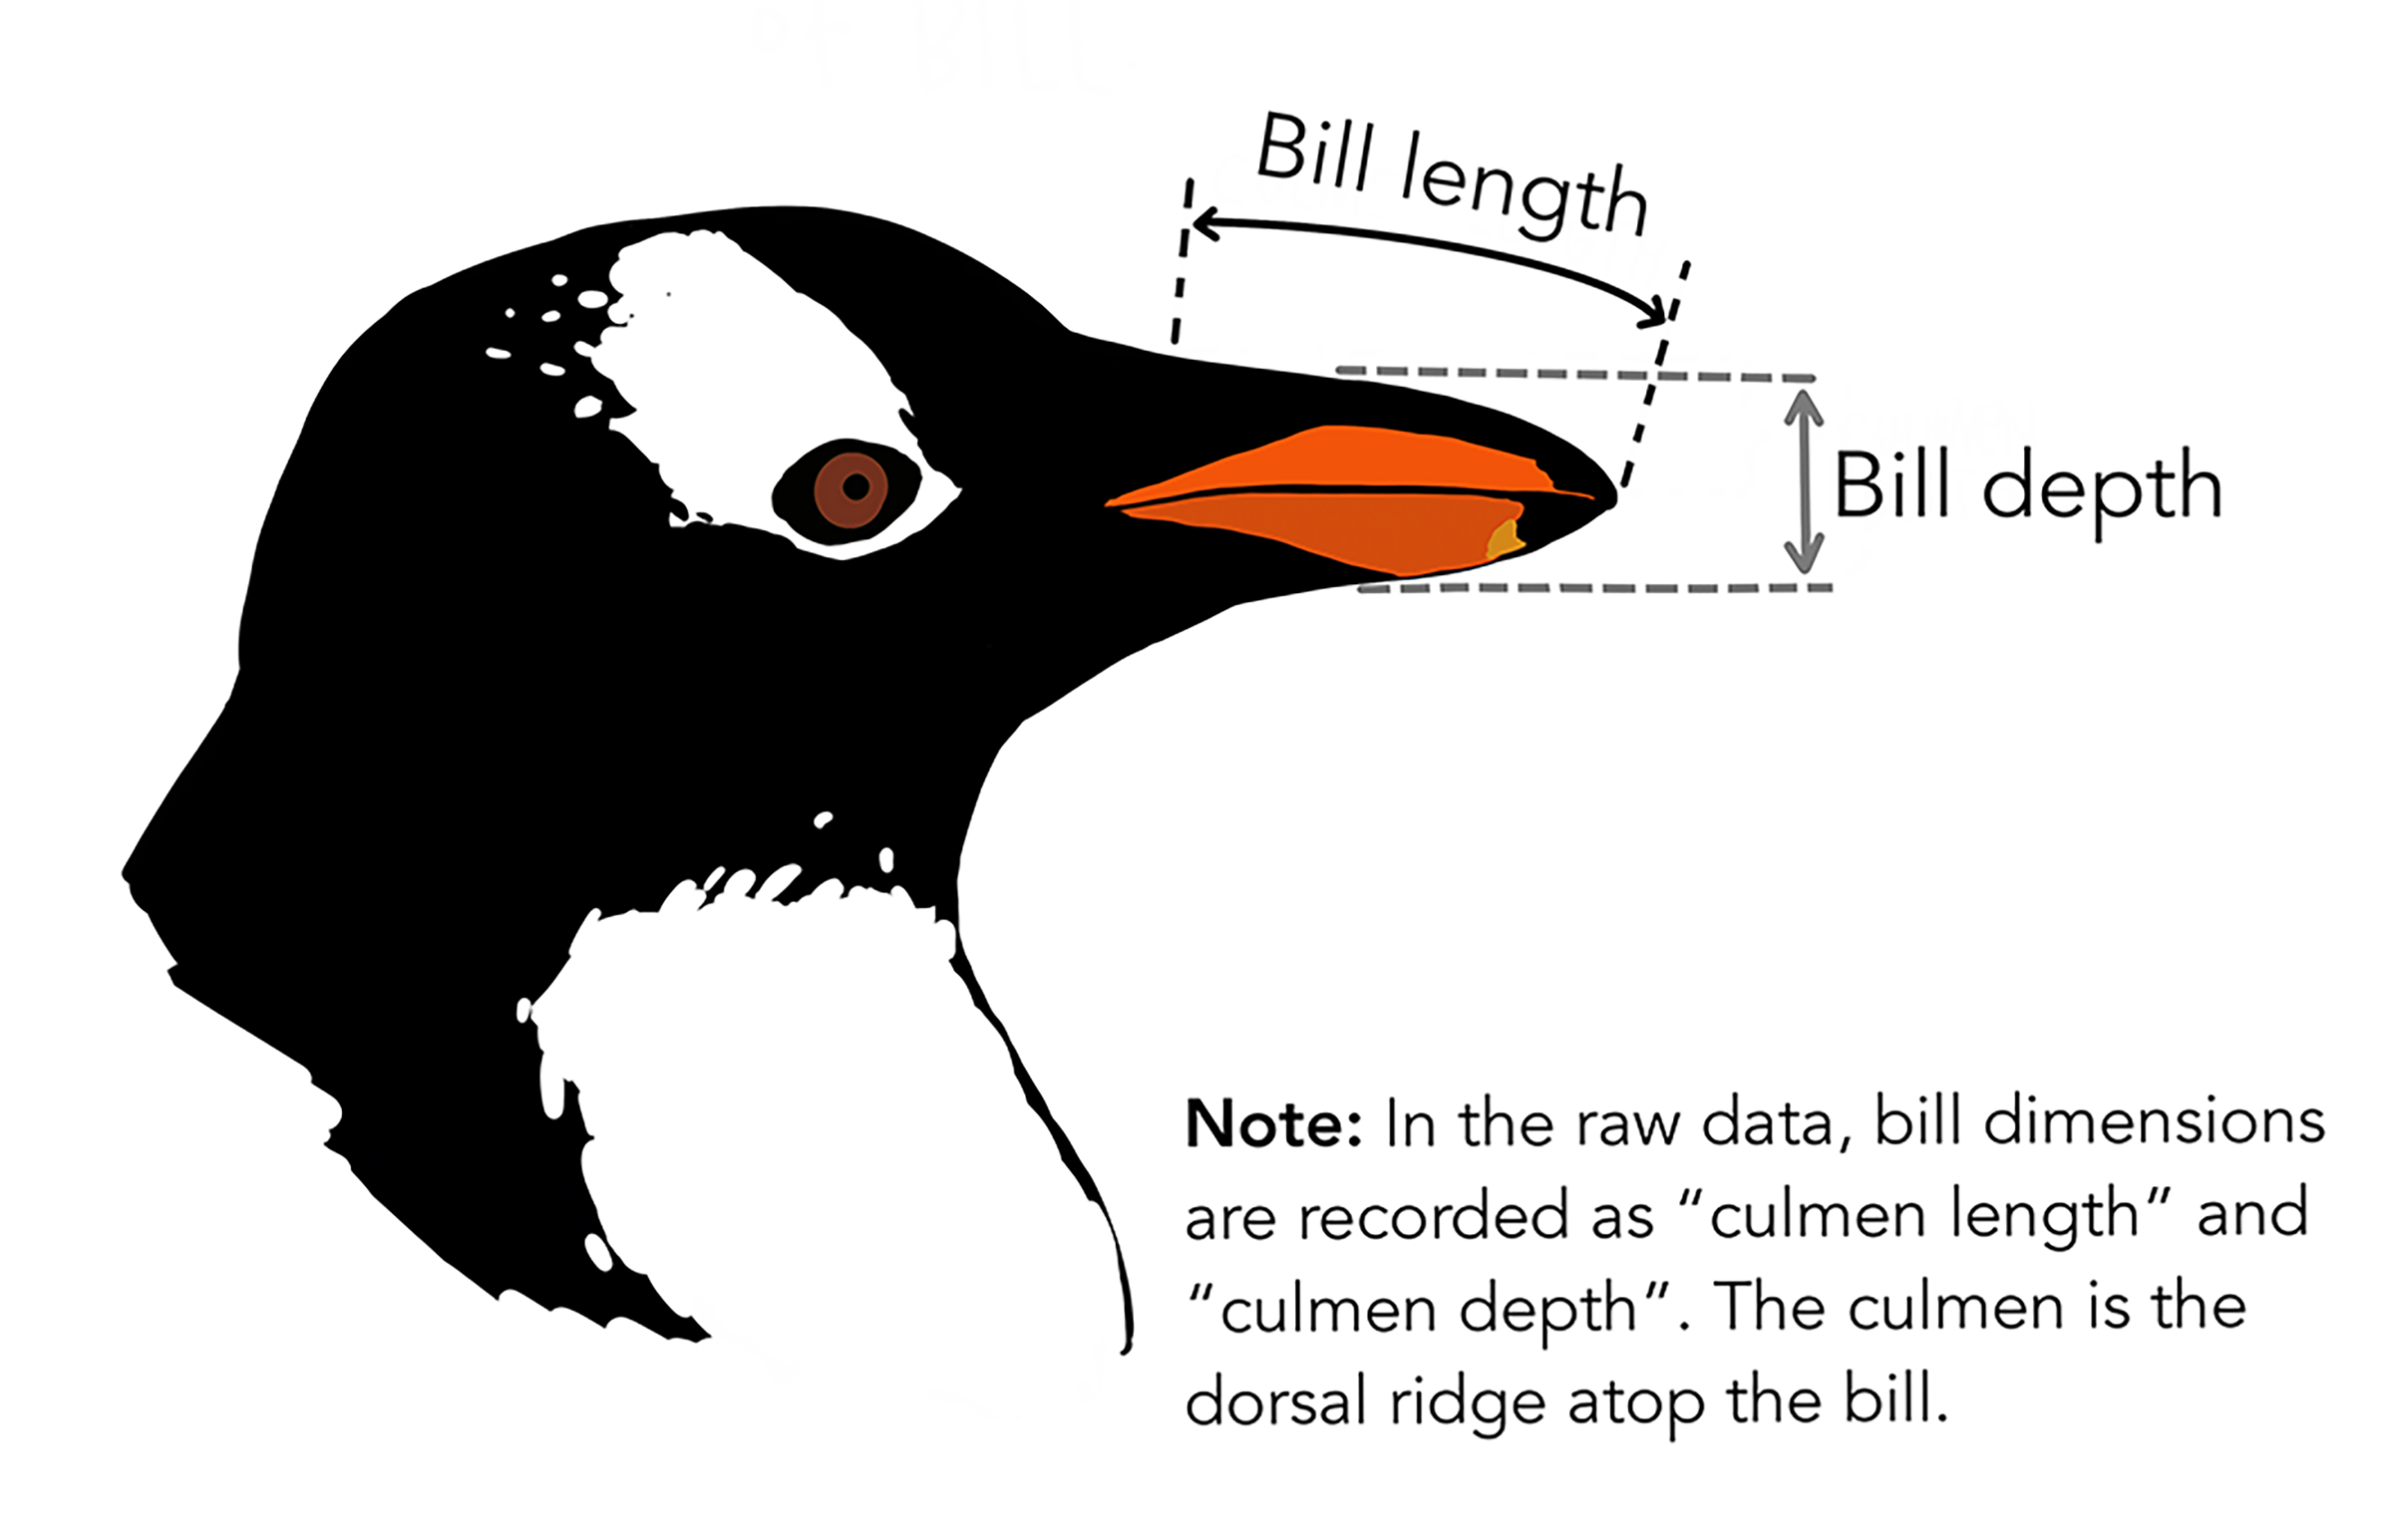
\includegraphics[width=0.6\linewidth]{img/culmen_depth_600dpi} 

}

\caption{Diagram of penguin head with indication of bill length and bill depth (from Horst, Hill, and Gorman (2020), used with permission)}\label{fig:introPenguinMorphometry}
\end{figure}

We'll use a couple of alternative \index{table display}table display methods, first a simple one\ldots{}

\begin{Shaded}
\begin{Highlighting}[]
\NormalTok{penguins}
\end{Highlighting}
\end{Shaded}

\begin{verbatim}
## # A tibble: 344 x 8
##    species island    bill_length_mm bill_depth_mm flipper_length_mm body_mass_g
##    <fct>   <fct>              <dbl>         <dbl>             <int>       <int>
##  1 Adelie  Torgersen           39.1          18.7               181        3750
##  2 Adelie  Torgersen           39.5          17.4               186        3800
##  3 Adelie  Torgersen           40.3          18                 195        3250
##  4 Adelie  Torgersen           NA            NA                  NA          NA
##  5 Adelie  Torgersen           36.7          19.3               193        3450
##  6 Adelie  Torgersen           39.3          20.6               190        3650
##  7 Adelie  Torgersen           38.9          17.8               181        3625
##  8 Adelie  Torgersen           39.2          19.6               195        4675
##  9 Adelie  Torgersen           34.1          18.1               193        3475
## 10 Adelie  Torgersen           42            20.2               190        4250
## # i 334 more rows
## # i 2 more variables: sex <fct>, year <int>
\end{verbatim}

\ldots{} then a nicer table display using \index{DT::datatable}\texttt{DT::datatable}, with a bit of improvement using an option\ldots{}

\begin{Shaded}
\begin{Highlighting}[]
\NormalTok{DT}\SpecialCharTok{::}\FunctionTok{datatable}\NormalTok{(penguins, }\AttributeTok{options=}\FunctionTok{list}\NormalTok{(}\AttributeTok{scrollX=}\NormalTok{T))}
\end{Highlighting}
\end{Shaded}

\begin{center}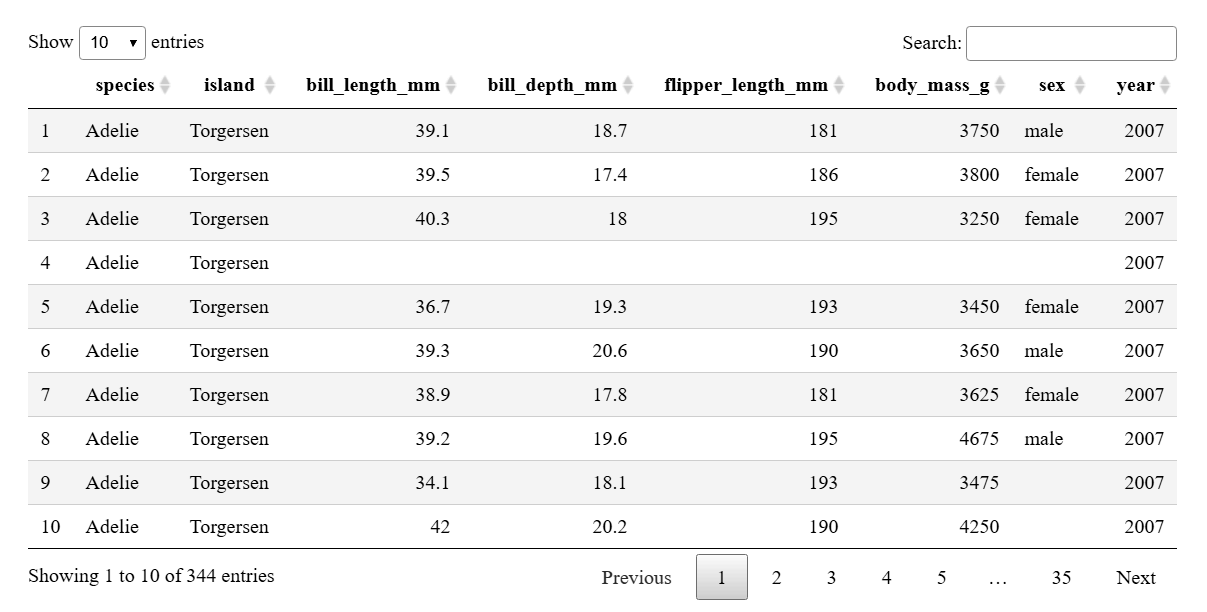
\includegraphics[width=1\linewidth]{img/penguinsDT} \end{center}

\subsubsection{Creating a data frame out of a matrix}\label{creating-a-data-frame-out-of-a-matrix}

\index{creating a data frame out of a matrix}There are many functions that start with \texttt{as.} that convert things to a desired type. We'll use \index{as.data.frame}\texttt{as.data.frame()} to create a data frame out of a matrix, the same \texttt{sierradata} we created earlier, but we'll build it again so it'll have variable names, and use yet another table display method from the \textbf{\texttt{knitr}} package (which also has a lot of options you might want to explore), which works well for both the html and pdf versions of this book, and creates numbered table headings, so I'll use it a lot (Table \ref{tab:introSierraKable}).

\begin{Shaded}
\begin{Highlighting}[]
\NormalTok{tC }\OtherTok{\textless{}{-}} \FunctionTok{c}\NormalTok{(}\FloatTok{10.7}\NormalTok{,  }\FloatTok{9.7}\NormalTok{,  }\FloatTok{7.7}\NormalTok{,  }\FloatTok{9.2}\NormalTok{,  }\FloatTok{7.3}\NormalTok{,  }\FloatTok{6.7}\NormalTok{,  }\FloatTok{4.0}\NormalTok{,  }\FloatTok{5.0}\NormalTok{,  }\FloatTok{0.9}\NormalTok{, }\SpecialCharTok{{-}}\FloatTok{1.1}\NormalTok{, }\SpecialCharTok{{-}}\FloatTok{0.8}\NormalTok{,}\SpecialCharTok{{-}}\FloatTok{4.4}\NormalTok{)}
\NormalTok{elev }\OtherTok{\textless{}{-}}   \FunctionTok{c}\NormalTok{(}\DecValTok{52}\NormalTok{,  }\DecValTok{394}\NormalTok{,  }\DecValTok{510}\NormalTok{,  }\DecValTok{564}\NormalTok{,  }\DecValTok{725}\NormalTok{,  }\DecValTok{848}\NormalTok{, }\DecValTok{1042}\NormalTok{, }\DecValTok{1225}\NormalTok{, }\DecValTok{1486}\NormalTok{, }\DecValTok{1775}\NormalTok{, }\DecValTok{1899}\NormalTok{, }\DecValTok{2551}\NormalTok{)}
\NormalTok{lat }\OtherTok{\textless{}{-}} \FunctionTok{c}\NormalTok{(}\FloatTok{39.52}\NormalTok{,}\FloatTok{38.91}\NormalTok{,}\FloatTok{37.97}\NormalTok{,}\FloatTok{38.70}\NormalTok{,}\FloatTok{39.09}\NormalTok{,}\FloatTok{39.25}\NormalTok{,}\FloatTok{39.94}\NormalTok{,}\FloatTok{37.75}\NormalTok{,}\FloatTok{40.35}\NormalTok{,}\FloatTok{39.33}\NormalTok{,}\FloatTok{39.17}\NormalTok{,}\FloatTok{38.21}\NormalTok{)}
\NormalTok{sierradata }\OtherTok{\textless{}{-}} \FunctionTok{cbind}\NormalTok{(tC, elev, lat)}
\NormalTok{sierradata }\OtherTok{\textless{}{-}} \FunctionTok{as.data.frame}\NormalTok{(sierradata) }\CommentTok{\# It\textquotesingle{}s ok to reuse the object name}
\NormalTok{knitr}\SpecialCharTok{::}\FunctionTok{kable}\NormalTok{(sierradata,}
  \AttributeTok{caption =} \StringTok{\textquotesingle{}Temperatures (Feb), elevations, and latitudes of 12 Sierra stations\textquotesingle{}}\NormalTok{)}
\end{Highlighting}
\end{Shaded}

\begin{table}

\caption{\label{tab:introSierraKable}Temperatures (Feb), elevations, and latitudes of 12 Sierra stations}
\centering
\begin{tabular}[t]{r|r|r}
\hline
tC & elev & lat\\
\hline
10.7 & 52 & 39.52\\
\hline
9.7 & 394 & 38.91\\
\hline
7.7 & 510 & 37.97\\
\hline
9.2 & 564 & 38.70\\
\hline
7.3 & 725 & 39.09\\
\hline
6.7 & 848 & 39.25\\
\hline
4.0 & 1042 & 39.94\\
\hline
5.0 & 1225 & 37.75\\
\hline
0.9 & 1486 & 40.35\\
\hline
-1.1 & 1775 & 39.33\\
\hline
-0.8 & 1899 & 39.17\\
\hline
-4.4 & 2551 & 38.21\\
\hline
\end{tabular}
\end{table}

Then to plot the two variables that are now part of the data frame, we'll need to make vectors out of them again using the accessor (Figure \ref{fig:introTempElev}).

\begin{Shaded}
\begin{Highlighting}[]
\FunctionTok{plot}\NormalTok{(sierradata}\SpecialCharTok{$}\NormalTok{elev, sierradata}\SpecialCharTok{$}\NormalTok{tC)}
\end{Highlighting}
\end{Shaded}

\begin{figure}

{\centering 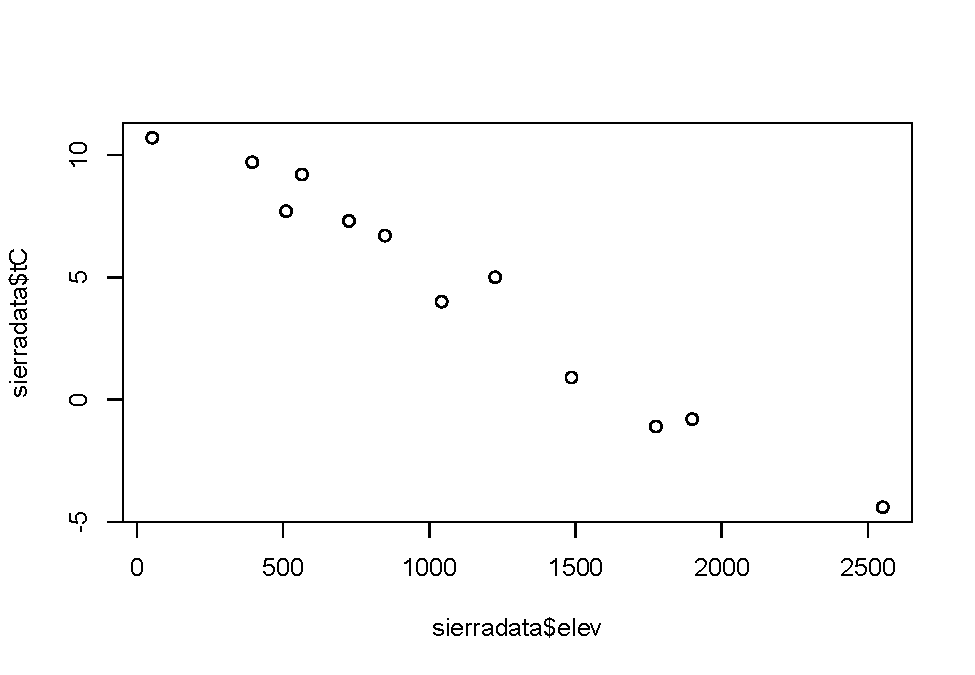
\includegraphics[width=0.75\linewidth]{EnvDataScience_files/figure-latex/introTempElev-1} 

}

\caption{Temperature and elevation scatter plot}\label{fig:introTempElev}
\end{figure}

\subsubsection{Creating a data frame directly from vectors}\label{creating-a-data-frame-directly-from-vectors}

We'll be using the \texttt{dplyr} package a lot in the next chapter, but we might as well introduce one of its functions -- \texttt{bind\_cols} -- that works a lot like \texttt{cbind} but creates data frames instead of matrices. Assuming we've already read in the vectors, we'd use this:

\begin{Shaded}
\begin{Highlighting}[]
\FunctionTok{library}\NormalTok{(tidyverse) }\CommentTok{\# includes the dplyr package}
\NormalTok{sierradata }\OtherTok{\textless{}{-}} \FunctionTok{bind\_cols}\NormalTok{(}\AttributeTok{tC=}\NormalTok{tC, }\AttributeTok{elev=}\NormalTok{elev,}\AttributeTok{lat=}\NormalTok{lat)}
\end{Highlighting}
\end{Shaded}

There are in fact multiple ways of creating data frames from vectors or other data. Here are a few examples that all use just one line of code.

\begin{Shaded}
\begin{Highlighting}[]
\NormalTok{sierradataD }\OtherTok{\textless{}{-}} \FunctionTok{as.data.frame}\NormalTok{(}\FunctionTok{cbind}\NormalTok{(tC,elev,lat))}
\NormalTok{sierradataE }\OtherTok{\textless{}{-}} \FunctionTok{data.frame}\NormalTok{(tC,elev,lat)}
\NormalTok{sierradataT }\OtherTok{\textless{}{-}} \FunctionTok{tibble}\NormalTok{(tC,elev,lat)}
\end{Highlighting}
\end{Shaded}

\begin{quote}
There are other ways to do this, but in general if you want a data frame, you should create it directly and not go through a matrix, as the first example above does. This one works fine but there are other situations where \texttt{cbind} won't end up with the right column names.
\end{quote}

\begin{quote}
Note that the last example above uses the \texttt{tibble} package, which is loaded with either \texttt{library(tibble)} or \texttt{library(tidyverse)}. We'll be looking at tibbles and other parts of the ``tidyverse'' more in the next chapter, but they're essentially an improved type of data frame.
\end{quote}

\subsubsection{Read a data frame from a CSV}\label{read-a-data-frame-from-a-csv}

\index{data frame from a CSV}We'll be looking at this more in the next chapter, but a common need is to read data from a spreadsheet stored in the CSV format. Normally, you'd have that stored with your project and can just specify the file name, but we'll access CSVs from the \index{igisci package}\texttt{igisci} package. Since you have this installed, it will already be on your computer, but not in your project folder. The path to it can be derived using the \texttt{system.file()} function.

Reading a csv in \index{readr}\texttt{readr} (part of the tidyverse that we'll be looking at in the next chapter) is done with \index{read csv}\texttt{read\_csv()}. We'll use the \texttt{DT::datatable} for this because it lets you interactively scroll across the many variables, and this table is included as Figure \ref{fig:introTRIDT}.

\begin{Shaded}
\begin{Highlighting}[]
\FunctionTok{library}\NormalTok{(readr)}
\NormalTok{csvPath }\OtherTok{\textless{}{-}} \FunctionTok{system.file}\NormalTok{(}\StringTok{"extdata"}\NormalTok{,}\StringTok{"TRI/TRI\_2017\_CA.csv"}\NormalTok{, }\AttributeTok{package=}\StringTok{"igisci"}\NormalTok{)}
\NormalTok{TRI2017 }\OtherTok{\textless{}{-}} \FunctionTok{read\_csv}\NormalTok{(csvPath)}
\end{Highlighting}
\end{Shaded}

\begin{Shaded}
\begin{Highlighting}[]
\NormalTok{DT}\SpecialCharTok{::}\FunctionTok{datatable}\NormalTok{(TRI2017, }\AttributeTok{options=}\FunctionTok{list}\NormalTok{(}\AttributeTok{scrollX=}\NormalTok{T))}
\end{Highlighting}
\end{Shaded}

\begin{figure}

{\centering 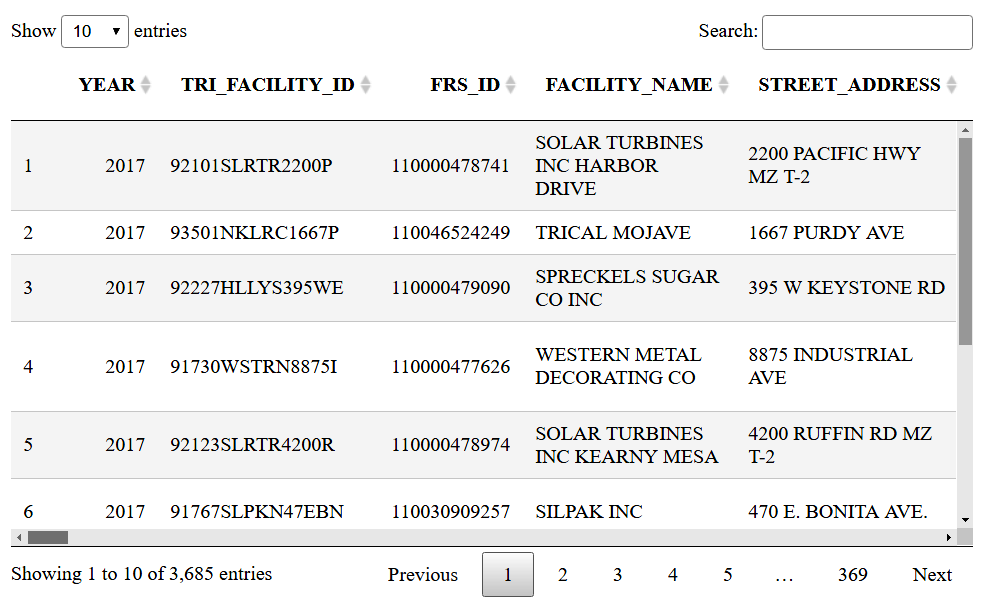
\includegraphics[width=1\linewidth]{img/TRI_DT} 

}

\caption{TRI dataframe -- DT datatable output}\label{fig:introTRIDT}
\end{figure}

Note that we could have used the built-in \texttt{read.csv} function, but as you'll see later, there are advantages of \texttt{readr::read\_csv} so we should get in the habit of using that instead.

\subsubsection{Reorganizing data frames}\label{reorganizing-data-frames}

There are quite a few ways to reorganize your data in R, and we'll learn other methods in the next chapter where we start using the tidyverse, which makes data abstraction and transformation much easier. For now, we'll work with a simpler CSV I've prepared:

\begin{Shaded}
\begin{Highlighting}[]
\NormalTok{csvPath }\OtherTok{\textless{}{-}} \FunctionTok{system.file}\NormalTok{(}\StringTok{"extdata"}\NormalTok{,}\StringTok{"TRI/TRI\_1987\_BaySites.csv"}\NormalTok{, }\AttributeTok{package=}\StringTok{"igisci"}\NormalTok{)}
\NormalTok{TRI87 }\OtherTok{\textless{}{-}} \FunctionTok{read\_csv}\NormalTok{(csvPath)}
\NormalTok{TRI87}
\end{Highlighting}
\end{Shaded}

\begin{verbatim}
## # A tibble: 335 x 9
##    TRI_FACILITY_ID count FACILITY_NAME          COUNTY air_releases fugitive_air
##    <chr>           <dbl> <chr>                  <chr>         <dbl>        <dbl>
##  1 91002FRMND585BR     2 FORUM IND              SAN M~         1423         1423
##  2 92052ZPMNF2970C     1 ZEP MFG CO             SANTA~          337          337
##  3 93117TLDYN3165P     2 TELEDYNE MEC           SANTA~        12600        12600
##  4 94002GTWSG477HA     2 MORGAN ADVANCED CERAM~ SAN M~        18700        18700
##  5 94002SMPRD120SE     2 SEM PRODS INC          SAN M~         1500          500
##  6 94025HBLNN151CO     2 HEUBLEIN INC           SAN M~          500            0
##  7 94025RYCHM300CO    10 TE CONNECTIVITY CORP   SAN M~       144871        47562
##  8 94025SNFRD990OB     1 SANFORD METAL PROCESS~ SAN M~         9675         9675
##  9 94026BYPCK3575H     2 BAY PACKAGING & CONVE~ SAN M~        80000        32000
## 10 94026CDRSY3475E     2 CDR SYS CORP           SAN M~       126800            0
## # i 325 more rows
## # i 3 more variables: stack_air <dbl>, LATITUDE <dbl>, LONGITUDE <dbl>
\end{verbatim}

\textbf{Sort, Index, and Max/Min}

One simple task is to \index{sort}sort data (numerically or by alphabetic order), such as a variable extracted as a vector.

\begin{Shaded}
\begin{Highlighting}[]
\FunctionTok{head}\NormalTok{(}\FunctionTok{sort}\NormalTok{(TRI87}\SpecialCharTok{$}\NormalTok{air\_releases))}
\end{Highlighting}
\end{Shaded}

\begin{verbatim}
## [1]  2  5  5  7  9 10
\end{verbatim}

\ldots{} or create an index vector of the \index{order}order of our vector/variable\ldots{}

\begin{Shaded}
\begin{Highlighting}[]
\NormalTok{index }\OtherTok{\textless{}{-}} \FunctionTok{order}\NormalTok{(TRI87}\SpecialCharTok{$}\NormalTok{air\_releases)}
\end{Highlighting}
\end{Shaded}

\ldots{} where the index vector is just used to store the order of the \texttt{TRI87\$air\_releases} vector/variable; then we can use that index to display facilities in order of their air releases.

\begin{Shaded}
\begin{Highlighting}[]
\FunctionTok{head}\NormalTok{(TRI87}\SpecialCharTok{$}\NormalTok{FACILITY\_NAME[index])}
\end{Highlighting}
\end{Shaded}

\begin{verbatim}
## [1] "AIR PRODUCTS MANUFACTURING CORP"         
## [2] "UNITED FIBERS"                           
## [3] "CLOROX MANUFACTURING CO"                 
## [4] "ICI AMERICAS INC WESTERN RESEARCH CENTER"
## [5] "UNION CARBIDE CORP"                      
## [6] "SCOTTS-SIERRA HORTICULTURAL PRODS CO INC"
\end{verbatim}

This is similar to filtering for a subset. We can also pull out individual values using functions like \texttt{which.max} to find the desired index value:

\begin{Shaded}
\begin{Highlighting}[]
\NormalTok{i\_max }\OtherTok{\textless{}{-}} \FunctionTok{which.max}\NormalTok{(TRI87}\SpecialCharTok{$}\NormalTok{air\_releases)}
\NormalTok{TRI87}\SpecialCharTok{$}\NormalTok{FACILITY\_NAME[i\_max]   }\CommentTok{\# was NUMMI at the time}
\end{Highlighting}
\end{Shaded}

\begin{verbatim}
## [1] "TESLA INC"
\end{verbatim}

\subsubsection{Length of a data frame}\label{length-of-a-data-frame}

You might expect the \texttt{length} of a data frame to be its number of rows, but it's the number of its variables. You'll get the same thing with \texttt{ncol}.

\begin{Shaded}
\begin{Highlighting}[]
\FunctionTok{length}\NormalTok{(TRI87)}
\FunctionTok{ncol}\NormalTok{(TRI87)}
\end{Highlighting}
\end{Shaded}

\begin{verbatim}
## [1] 9
## [1] 9
\end{verbatim}

To get the number of rows, you can access a single variable as a vector, or you can use \texttt{nrow}.

\begin{Shaded}
\begin{Highlighting}[]
\FunctionTok{length}\NormalTok{(TRI87}\SpecialCharTok{$}\NormalTok{count)}
\FunctionTok{nrow}\NormalTok{(TRI87)}
\end{Highlighting}
\end{Shaded}

\begin{verbatim}
## [1] 335
## [1] 335
\end{verbatim}

\subsection{Factors}\label{factors}

\index{factors}Factors are vectors with predefined values, normally used for categorical data, and as R is a statistical language are frequently used to stratify data, such as defining groups for analysis of variance among those groups. They are built on an \emph{integer} vector, and \index{factor levels}\emph{levels} are the set of predefined values, which are commonly character data.

\begin{Shaded}
\begin{Highlighting}[]
\NormalTok{nut }\OtherTok{\textless{}{-}} \FunctionTok{factor}\NormalTok{(}\FunctionTok{c}\NormalTok{(}\StringTok{"almond"}\NormalTok{, }\StringTok{"walnut"}\NormalTok{, }\StringTok{"pecan"}\NormalTok{, }\StringTok{"almond"}\NormalTok{))}
\FunctionTok{str}\NormalTok{(nut)   }\CommentTok{\# note that levels will be in alphabetical order}
\end{Highlighting}
\end{Shaded}

\begin{verbatim}
##  Factor w/ 3 levels "almond","pecan",..: 1 3 2 1
\end{verbatim}

\begin{Shaded}
\begin{Highlighting}[]
\FunctionTok{typeof}\NormalTok{(nut)}
\end{Highlighting}
\end{Shaded}

\begin{verbatim}
## [1] "integer"
\end{verbatim}

As always, there are multiple ways of doing things. Here's an equivalent conversion that illustrates their relation to integers:

\begin{Shaded}
\begin{Highlighting}[]
\NormalTok{nutint }\OtherTok{\textless{}{-}} \FunctionTok{c}\NormalTok{(}\DecValTok{1}\NormalTok{, }\DecValTok{2}\NormalTok{, }\DecValTok{3}\NormalTok{, }\DecValTok{2}\NormalTok{) }\CommentTok{\# equivalent conversion}
\NormalTok{nut }\OtherTok{\textless{}{-}} \FunctionTok{factor}\NormalTok{(nutint, }\AttributeTok{labels =} \FunctionTok{c}\NormalTok{(}\StringTok{"almond"}\NormalTok{, }\StringTok{"pecan"}\NormalTok{, }\StringTok{"walnut"}\NormalTok{))}
\FunctionTok{str}\NormalTok{(nut)}
\end{Highlighting}
\end{Shaded}

\begin{verbatim}
##  Factor w/ 3 levels "almond","pecan",..: 1 2 3 2
\end{verbatim}

\subsubsection{Categorical data and factors}\label{categorical-data-and-factors}

\index{categorical data and factors}While character data might be seen as categorical (e.g.~\texttt{"urban"}, \texttt{"agricultural"}, \texttt{"forest"} land covers), to be used as categorical variables they must be made into factors. So we have something to work with, we'll generate some \index{random}random memberships in one of three vegetation moisture categories using the \index{sample}\texttt{sample()} function:

\begin{Shaded}
\begin{Highlighting}[]
\NormalTok{veg\_moisture\_categories }\OtherTok{\textless{}{-}} \FunctionTok{c}\NormalTok{(}\StringTok{"xeric"}\NormalTok{, }\StringTok{"mesic"}\NormalTok{, }\StringTok{"hydric"}\NormalTok{)}
\NormalTok{veg\_moisture\_char }\OtherTok{\textless{}{-}} \FunctionTok{sample}\NormalTok{(veg\_moisture\_categories, }\DecValTok{42}\NormalTok{, }\AttributeTok{replace =} \ConstantTok{TRUE}\NormalTok{)}
\NormalTok{veg\_moisture\_fact }\OtherTok{\textless{}{-}} \FunctionTok{factor}\NormalTok{(veg\_moisture\_char, }\AttributeTok{levels =}\NormalTok{ veg\_moisture\_categories)}
\NormalTok{veg\_moisture\_char}
\end{Highlighting}
\end{Shaded}

\begin{verbatim}
##  [1] "hydric" "xeric"  "mesic"  "mesic"  "hydric" "mesic"  "hydric" "hydric"
##  [9] "hydric" "mesic"  "hydric" "hydric" "hydric" "mesic"  "hydric" "xeric" 
## [17] "hydric" "hydric" "mesic"  "hydric" "mesic"  "xeric"  "hydric" "mesic" 
## [25] "mesic"  "mesic"  "hydric" "xeric"  "mesic"  "hydric" "xeric"  "mesic" 
## [33] "mesic"  "hydric" "mesic"  "mesic"  "hydric" "mesic"  "mesic"  "xeric" 
## [41] "hydric" "xeric"
\end{verbatim}

\begin{Shaded}
\begin{Highlighting}[]
\NormalTok{veg\_moisture\_fact}
\end{Highlighting}
\end{Shaded}

\begin{verbatim}
##  [1] hydric xeric  mesic  mesic  hydric mesic  hydric hydric hydric mesic 
## [11] hydric hydric hydric mesic  hydric xeric  hydric hydric mesic  hydric
## [21] mesic  xeric  hydric mesic  mesic  mesic  hydric xeric  mesic  hydric
## [31] xeric  mesic  mesic  hydric mesic  mesic  hydric mesic  mesic  xeric 
## [41] hydric xeric 
## Levels: xeric mesic hydric
\end{verbatim}

To make a categorical variable a factor:

\begin{Shaded}
\begin{Highlighting}[]
\NormalTok{nut }\OtherTok{\textless{}{-}} \FunctionTok{c}\NormalTok{(}\StringTok{"almond"}\NormalTok{, }\StringTok{"walnut"}\NormalTok{, }\StringTok{"pecan"}\NormalTok{, }\StringTok{"almond"}\NormalTok{)}
\NormalTok{farm }\OtherTok{\textless{}{-}} \FunctionTok{c}\NormalTok{(}\StringTok{"organic"}\NormalTok{, }\StringTok{"conventional"}\NormalTok{, }\StringTok{"organic"}\NormalTok{, }\StringTok{"organic"}\NormalTok{)}
\NormalTok{ag }\OtherTok{\textless{}{-}} \FunctionTok{as.data.frame}\NormalTok{(}\FunctionTok{cbind}\NormalTok{(nut, farm))}
\NormalTok{ag}\SpecialCharTok{$}\NormalTok{nut }\OtherTok{\textless{}{-}} \FunctionTok{factor}\NormalTok{(ag}\SpecialCharTok{$}\NormalTok{nut)}
\NormalTok{ag}\SpecialCharTok{$}\NormalTok{nut}
\end{Highlighting}
\end{Shaded}

\begin{verbatim}
## [1] almond walnut pecan  almond
## Levels: almond pecan walnut
\end{verbatim}

\textbf{Factor example}

\begin{Shaded}
\begin{Highlighting}[]
\FunctionTok{library}\NormalTok{(igisci)}
\NormalTok{sierraFeb}\SpecialCharTok{$}\NormalTok{COUNTY }\OtherTok{\textless{}{-}} \FunctionTok{factor}\NormalTok{(sierraFeb}\SpecialCharTok{$}\NormalTok{COUNTY)}
\FunctionTok{str}\NormalTok{(sierraFeb}\SpecialCharTok{$}\NormalTok{COUNTY)}
\end{Highlighting}
\end{Shaded}

\begin{verbatim}
##  Factor w/ 21 levels "Amador","Butte",..: 20 14 7 12 12 2 19 11 2 19 ...
\end{verbatim}

\section{Accessors and Subsetting}\label{accessors}

The use of \index{accessors}\emph{accessors} in R can be confusing, but they're very important to understand. An accessor is ``a method for accessing data in an object usually an attribute of that object'' (Brown (\citeproc{ref-Brown_R_accessors}{n.d.})), so a method for subsetting, and for R these are \index{`[ ]` accessor}\textbf{\texttt{{[}{]}}}, \index{`[[ ]]` accessor}\textbf{\texttt{{[}{[}{]}{]}}}, and \index{\$ accessor}\textbf{\texttt{\$}}, but it can be confusing to know when you might use which one. There are good reasons to have these three types for code clarity, however you can also use \textbf{\texttt{{[}{]}}} with a bit of clumsiness for all purposes.

We've already been using these in this chapter and will continue to use them throughout the book. Let's look at the various accessors and subsetting options:

\subsection{\texorpdfstring{\texttt{{[}{]}} Subsetting}{{[}{]} Subsetting}}\label{subsetting}

\index{subsetting}You use this to get a subset of any R object, whether it be a vector, list, or data frame. For a vector, the subset might be defined by indices \ldots{}

\begin{Shaded}
\begin{Highlighting}[]
\NormalTok{lats }\OtherTok{\textless{}{-}} \FunctionTok{c}\NormalTok{(}\FloatTok{37.5}\NormalTok{,}\FloatTok{47.4}\NormalTok{,}\FloatTok{29.4}\NormalTok{,}\FloatTok{33.4}\NormalTok{)}
\FunctionTok{str}\NormalTok{(lats[}\DecValTok{4}\NormalTok{])}
\end{Highlighting}
\end{Shaded}

\begin{verbatim}
##  num 33.4
\end{verbatim}

\begin{Shaded}
\begin{Highlighting}[]
\FunctionTok{str}\NormalTok{(lats[}\DecValTok{2}\SpecialCharTok{:}\DecValTok{3}\NormalTok{])}
\end{Highlighting}
\end{Shaded}

\begin{verbatim}
##  num [1:2] 47.4 29.4
\end{verbatim}

\begin{Shaded}
\begin{Highlighting}[]
\FunctionTok{str}\NormalTok{(letters[}\DecValTok{24}\SpecialCharTok{:}\DecValTok{26}\NormalTok{])}
\end{Highlighting}
\end{Shaded}

\begin{verbatim}
##  chr [1:3] "x" "y" "z"
\end{verbatim}

\ldots{} or a \index{Boolean}Boolean with \texttt{TRUE} or \texttt{FALSE} values representing which to keep or not.

\begin{Shaded}
\begin{Highlighting}[]
\FunctionTok{str}\NormalTok{(lats[}\FunctionTok{c}\NormalTok{(}\ConstantTok{TRUE}\NormalTok{,}\ConstantTok{FALSE}\NormalTok{,}\ConstantTok{TRUE}\NormalTok{,}\ConstantTok{TRUE}\NormalTok{)])}
\end{Highlighting}
\end{Shaded}

\begin{verbatim}
##  num [1:3] 37.5 29.4 33.4
\end{verbatim}

An initially surprising but very handy way of creating one of these is to \emph{reference the vector itself} in a relational expression. The following returns the same as the above, with the purpose of selecting all lats that are less than 40:

\begin{Shaded}
\begin{Highlighting}[]
\FunctionTok{str}\NormalTok{(lats[lats}\SpecialCharTok{\textless{}}\DecValTok{40}\NormalTok{])}
\end{Highlighting}
\end{Shaded}

\begin{verbatim}
##  num [1:3] 37.5 29.4 33.4
\end{verbatim}

Getting one element from a data frame will return a data frame, in this case a data frame with just one variable. For columns especially, you might expect the result to be a vector, but it's a data frame with just one variable. Note that you can use either the column number or the name of the variable.

\begin{Shaded}
\begin{Highlighting}[]
\FunctionTok{str}\NormalTok{(cars)}
\end{Highlighting}
\end{Shaded}

\begin{verbatim}
## 'data.frame':    50 obs. of  2 variables:
##  $ speed: num  4 4 7 7 8 9 10 10 10 11 ...
##  $ dist : num  2 10 4 22 16 10 18 26 34 17 ...
\end{verbatim}

\begin{Shaded}
\begin{Highlighting}[]
\FunctionTok{str}\NormalTok{(cars[}\DecValTok{1}\NormalTok{])}
\end{Highlighting}
\end{Shaded}

\begin{verbatim}
## 'data.frame':    50 obs. of  1 variable:
##  $ speed: num  4 4 7 7 8 9 10 10 10 11 ...
\end{verbatim}

\begin{Shaded}
\begin{Highlighting}[]
\FunctionTok{str}\NormalTok{(cars[}\StringTok{"speed"}\NormalTok{])}
\end{Highlighting}
\end{Shaded}

\begin{verbatim}
## 'data.frame':    50 obs. of  1 variable:
##  $ speed: num  4 4 7 7 8 9 10 10 10 11 ...
\end{verbatim}

Similarly, subsetting to get a single \emph{observation} (a row of values) with the \texttt{{[}n,{]}} method returns a one-row data frame, or it can be used to create a subset of a range or selection of observations. You can also get all but a given observation with \texttt{{[}-n,{]}}.

\begin{Shaded}
\begin{Highlighting}[]
\NormalTok{cars[}\DecValTok{1}\NormalTok{,]}
\end{Highlighting}
\end{Shaded}

\begin{verbatim}
##   speed dist
## 1     4    2
\end{verbatim}

\begin{Shaded}
\begin{Highlighting}[]
\NormalTok{cars[}\DecValTok{3}\SpecialCharTok{:}\DecValTok{5}\NormalTok{,]}
\end{Highlighting}
\end{Shaded}

\begin{verbatim}
##   speed dist
## 3     7    4
## 4     7   22
## 5     8   16
\end{verbatim}

\begin{Shaded}
\begin{Highlighting}[]
\NormalTok{cars[}\SpecialCharTok{{-}}\DecValTok{2}\NormalTok{,]}
\end{Highlighting}
\end{Shaded}

\begin{verbatim}
##    speed dist
## 1      4    2
## 3      7    4
## 4      7   22
## 5      8   16
## 6      9   10
## 7     10   18
## 8     10   26
## 9     10   34
## 10    11   17
## 11    11   28
## 12    12   14
## 13    12   20
## 14    12   24
## 15    12   28
## 16    13   26
## 17    13   34
## 18    13   34
## 19    13   46
## 20    14   26
## 21    14   36
## 22    14   60
## 23    14   80
## 24    15   20
## 25    15   26
## 26    15   54
## 27    16   32
## 28    16   40
## 29    17   32
## 30    17   40
## 31    17   50
## 32    18   42
## 33    18   56
## 34    18   76
## 35    18   84
## 36    19   36
## 37    19   46
## 38    19   68
## 39    20   32
## 40    20   48
## 41    20   52
## 42    20   56
## 43    20   64
## 44    22   66
## 45    23   54
## 46    24   70
## 47    24   92
## 48    24   93
## 49    24  120
## 50    25   85
\end{verbatim}

\begin{Shaded}
\begin{Highlighting}[]
\NormalTok{cars[cars[}\StringTok{"speed"}\NormalTok{]}\SpecialCharTok{\textless{}}\DecValTok{10}\NormalTok{,]}
\end{Highlighting}
\end{Shaded}

\begin{verbatim}
##   speed dist
## 1     4    2
## 2     4   10
## 3     7    4
## 4     7   22
## 5     8   16
## 6     9   10
\end{verbatim}

\emph{Getting a data frame this way is very useful because many functions you'll want to use require a data frame as input.}

But sometimes you just want a vector. If you select an individual variable using the \texttt{{[},n{]}} method, you'll get one. You'll want to assign it to a meaningful name like the original variable name. Note that you can either use the variable name or the variable column number:

\begin{Shaded}
\begin{Highlighting}[]
\NormalTok{dist }\OtherTok{\textless{}{-}}\NormalTok{ cars[,}\StringTok{"dist"}\NormalTok{] }\CommentTok{\# or cars[,2]}
\NormalTok{dist}
\end{Highlighting}
\end{Shaded}

\begin{verbatim}
##  [1]   2  10   4  22  16  10  18  26  34  17  28  14  20  24  28  26  34  34  46
## [20]  26  36  60  80  20  26  54  32  40  32  40  50  42  56  76  84  36  46  68
## [39]  32  48  52  56  64  66  54  70  92  93 120  85
\end{verbatim}

\subsection{\texorpdfstring{\texttt{{[}{[}{]}{]}} The mysterious double bracket}{{[}{[}{]}{]} The mysterious double bracket}}\label{the-mysterious-double-bracket}

\index{`[[ ]]` accessor}Double brackets extract just one element, so just one value from a vector or one vector from a data frame. You're going one step further into the structure.

\begin{Shaded}
\begin{Highlighting}[]
\FunctionTok{str}\NormalTok{(cars[,}\StringTok{"speed"}\NormalTok{])}
\end{Highlighting}
\end{Shaded}

\begin{verbatim}
##  num [1:50] 4 4 7 7 8 9 10 10 10 11 ...
\end{verbatim}

\begin{Shaded}
\begin{Highlighting}[]
\FunctionTok{str}\NormalTok{(cars[[}\StringTok{"speed"}\NormalTok{]])}
\end{Highlighting}
\end{Shaded}

\begin{verbatim}
##  num [1:50] 4 4 7 7 8 9 10 10 10 11 ...
\end{verbatim}

Note that the str result is telling you that these are both simply vectors, not something like a data frame. Though uncommon, you can also use the index of variables instead of its name. Similar to the examples above, the variable can be specified either with the index (or column number) or the variable name. Since ``speed'' is the first variable in the cars data frame, these return the same thing:

\begin{Shaded}
\begin{Highlighting}[]
\FunctionTok{str}\NormalTok{(cars[[}\DecValTok{1}\NormalTok{]])}
\end{Highlighting}
\end{Shaded}

\begin{verbatim}
##  num [1:50] 4 4 7 7 8 9 10 10 10 11 ...
\end{verbatim}

\begin{Shaded}
\begin{Highlighting}[]
\FunctionTok{str}\NormalTok{(cars[[}\StringTok{"speed"}\NormalTok{]])}
\end{Highlighting}
\end{Shaded}

\begin{verbatim}
##  num [1:50] 4 4 7 7 8 9 10 10 10 11 ...
\end{verbatim}

\subsection{\texorpdfstring{\texttt{\$} Accessing a vector from a data frame}{\$ Accessing a vector from a data frame}}\label{accessing-a-vector-from-a-data-frame}

The \index{\$ accessor}\texttt{\$} accessor is really just a shortcut, but any shortcut reduces code and thus increases clarity, so it's a good idea and this accessor is commonly used. Their only limitation is that you can't use the integer indices, which would allow you to loop through a numerical sequence.

These accessor operations do the same thing:

\begin{Shaded}
\begin{Highlighting}[]
\NormalTok{cars}\SpecialCharTok{$}\NormalTok{speed}
\NormalTok{cars[,}\StringTok{"speed"}\NormalTok{]}
\NormalTok{cars[[}\StringTok{"speed"}\NormalTok{]]}
\end{Highlighting}
\end{Shaded}

\begin{verbatim}
##  num [1:50] 4 4 7 7 8 9 10 10 10 11 ...
\end{verbatim}

Again, to contrast, the following accessor operations do the same thing -- create a data frame:

\begin{Shaded}
\begin{Highlighting}[]
\NormalTok{sp1 }\OtherTok{\textless{}{-}}\NormalTok{ cars[}\DecValTok{1}\NormalTok{] }\CommentTok{\# gets the first variable, "speed"}
\NormalTok{sp2 }\OtherTok{\textless{}{-}}\NormalTok{ cars[}\StringTok{"speed"}\NormalTok{]}
\FunctionTok{str}\NormalTok{(sp1)}
\end{Highlighting}
\end{Shaded}

\begin{verbatim}
## 'data.frame':    50 obs. of  1 variable:
##  $ speed: num  4 4 7 7 8 9 10 10 10 11 ...
\end{verbatim}

\begin{Shaded}
\begin{Highlighting}[]
\FunctionTok{identical}\NormalTok{(sp1,sp2)}
\end{Highlighting}
\end{Shaded}

\begin{verbatim}
## [1] TRUE
\end{verbatim}

\section{Programming scripts in RStudio}\label{programming}

\index{programming scripts in RStudio}Given the exploratory nature of the R language, we sometimes forget that it provides significant capabilities as a programming language where we can solve more complex problems by coding procedures and using logic to control the process and handle a range of possible scenarios.

Programming languages are used for a wide range of purposes, from developing operating systems built from low-level code to high-level \index{scripting}\emph{scripting} used to run existing functions in libraries. R and Python are commonly used for scripting, and you may be familiar with using \index{arcpy}arcpy to script \index{ArcGIS}ArcGIS geoprocessing tools. But whether low- or high-level, some common \index{operational structures}operational structures are used in all computer programming languages:

\begin{itemize}
\tightlist
\item
  functions (defining your own)
\item
  conditional operations: \emph{if} a condition is true, \emph{do this}
\item
  loops
\end{itemize}

Common to all of these is an input in parentheses followed by what to do in braces:

\begin{itemize}
\tightlist
\item
  \emph{obj} \texttt{\textless{}-\ function(}\emph{input}\texttt{)\{}\emph{process ending in an expression result}\texttt{\}}
\item
  \texttt{if(}\emph{condition}\texttt{)\{}\emph{process}\texttt{\}}
\item
  \texttt{if(}\emph{condition}\texttt{)\{}\emph{process}\texttt{\}\ else\ \{}\emph{process}\texttt{\}}
\item
  \texttt{for(}\emph{object}\texttt{in}\emph{list}\texttt{)\{}\emph{process}\texttt{\}}
\end{itemize}

The \texttt{\{\ \}} braces are only needed if the process goes past the first line, so for instance the following examples don't need them (and actually some of the spaces aren't necessary either, but I left them in for clarity):

\begin{Shaded}
\begin{Highlighting}[]
\NormalTok{a }\OtherTok{\textless{}{-}} \DecValTok{2}
\NormalTok{f }\OtherTok{\textless{}{-}} \ControlFlowTok{function}\NormalTok{(a) a}\SpecialCharTok{*}\DecValTok{2}
\FunctionTok{print}\NormalTok{(}\FunctionTok{f}\NormalTok{(}\DecValTok{4}\NormalTok{))}
\ControlFlowTok{if}\NormalTok{(a}\SpecialCharTok{==}\DecValTok{3}\NormalTok{) }\FunctionTok{print}\NormalTok{(}\StringTok{\textquotesingle{}yes\textquotesingle{}}\NormalTok{) }\ControlFlowTok{else} \FunctionTok{print}\NormalTok{(}\StringTok{\textquotesingle{}no\textquotesingle{}}\NormalTok{)}
\ControlFlowTok{for}\NormalTok{(i }\ControlFlowTok{in} \DecValTok{1}\SpecialCharTok{:}\DecValTok{5}\NormalTok{) }\FunctionTok{print}\NormalTok{(i)}
\end{Highlighting}
\end{Shaded}

\subsection{\texorpdfstring{\texttt{function} : creating your own}{function : creating your own}}\label{functions-writing}

\texttt{myFunction\ \textless{}-\ function(input)\{}\emph{Do this and return the resulting expression}\texttt{\}}

\index{functions}The various packages that we're installing, all those that aren't purely data (like \texttt{igisci}), are built primarily of functions and perhaps most of those functions are written in R. Many of these simply make existing R functions work better or at least differently, often for a particular data science task commonly needed in a discipline or application area.

In geospatial environmental research for instance, we are often dealing with direction, for instance the movement of marine mammals who might be influenced by ship traffic. An agent-based model simulation of marine mammal movement might have the animal respond by shifting to the left or right, so we might want a \texttt{turnLeft()} or \texttt{turnRight()} function. Given the nature of circular data however, the code might be sufficiently complex to warrant writing a function that will make our main code easier to read:

\begin{Shaded}
\begin{Highlighting}[]
\NormalTok{turnright }\OtherTok{\textless{}{-}} \ControlFlowTok{function}\NormalTok{(ang)\{(ang }\SpecialCharTok{+} \DecValTok{90}\NormalTok{) }\SpecialCharTok{\%\%} \DecValTok{360}\NormalTok{\}}
\end{Highlighting}
\end{Shaded}

Then in our code later on, after we've prepared some data \ldots{}

\begin{Shaded}
\begin{Highlighting}[]
\NormalTok{id }\OtherTok{\textless{}{-}} \FunctionTok{c}\NormalTok{(}\StringTok{"5A"}\NormalTok{, }\StringTok{"12D"}\NormalTok{, }\StringTok{"3B"}\NormalTok{)}
\NormalTok{direction }\OtherTok{\textless{}{-}} \FunctionTok{c}\NormalTok{(}\DecValTok{260}\NormalTok{, }\DecValTok{270}\NormalTok{, }\DecValTok{300}\NormalTok{)}
\NormalTok{whale }\OtherTok{\textless{}{-}}\NormalTok{ dplyr}\SpecialCharTok{::}\FunctionTok{bind\_cols}\NormalTok{(}\AttributeTok{id =}\NormalTok{ id,}\AttributeTok{direction =}\NormalTok{ direction) }\CommentTok{\# better than cbind}
\NormalTok{whale}
\end{Highlighting}
\end{Shaded}

\begin{verbatim}
## # A tibble: 3 x 2
##   id    direction
##   <chr>     <dbl>
## 1 5A          260
## 2 12D         270
## 3 3B          300
\end{verbatim}

\ldots{} we can call this function:

\begin{Shaded}
\begin{Highlighting}[]
\NormalTok{whale}\SpecialCharTok{$}\NormalTok{direction }\OtherTok{\textless{}{-}} \FunctionTok{turnright}\NormalTok{(whale}\SpecialCharTok{$}\NormalTok{direction)}
\NormalTok{whale}
\end{Highlighting}
\end{Shaded}

\begin{verbatim}
## # A tibble: 3 x 2
##   id    direction
##   <chr>     <dbl>
## 1 5A          350
## 2 12D           0
## 3 3B           30
\end{verbatim}

Another function I found useful for our external data in \texttt{igisci} is to simplify the code needed to access the external data. I found I had to keep looking up the syntax for that task that we use a lot. It also makes the code difficult to read. Adding this function to the top of your code helps for both:

\begin{Shaded}
\begin{Highlighting}[]
\NormalTok{ex }\OtherTok{\textless{}{-}} \ControlFlowTok{function}\NormalTok{(fnam)\{}\FunctionTok{system.file}\NormalTok{(}\StringTok{"extdata"}\NormalTok{,fnam,}\AttributeTok{package=}\StringTok{"igisci"}\NormalTok{)\}}
\end{Highlighting}
\end{Shaded}

Then our code that accesses data is greatly simplified, with \texttt{read.csv} calls looking a lot like reading data stored in our project folder. For example, where if we had \texttt{fishdata.csv} stored locally in our project folder we might read it with \ldots{}

\texttt{read.csv("fishdata.csv")}

\ldots{} reading from the data package's extdata folder looks pretty similar:

\texttt{read.csv(ex("fishdata.csv"))}

\begin{quote}
This simple function was so useful that it's now included in the igisci package, so you can just call it with \texttt{ex()} if you have \texttt{library(igisci)} in your code.
\end{quote}

\subsection{\texorpdfstring{\texttt{if} : conditional operations}{if : conditional operations}}\label{if-conditional-operations}

\texttt{if\ (condition)\ \{}\emph{Do this}\texttt{\}\ else\ \{}\emph{Do this other thing}\texttt{\}}

\index{if else}Probably not used as much in R for most users, as it's mostly useful for building a new tool (or function) that needs to run as a complete operation. (But I found it essential in writing this book to create some outputs differently for the output to html than for the output to LaTeX for the pdf/book version.)

Common in coding is the need to be able to handle a variety of inputs and \emph{avoid errors}. Here's an admittedly trivial example of some short code that avoids an error:

\begin{Shaded}
\begin{Highlighting}[]
\NormalTok{getRatio }\OtherTok{\textless{}{-}} \ControlFlowTok{function}\NormalTok{(x,y)\{}
  \ControlFlowTok{if}\NormalTok{ (y}\SpecialCharTok{!=}\DecValTok{0}\NormalTok{)\{x}\SpecialCharTok{/}\NormalTok{y\} }\ControlFlowTok{else}\NormalTok{ \{}\FloatTok{1e1000}\NormalTok{\}}
\NormalTok{\}}

\FunctionTok{getRatio}\NormalTok{(}\DecValTok{5}\NormalTok{,}\DecValTok{0}\NormalTok{)}
\end{Highlighting}
\end{Shaded}

\begin{verbatim}
## [1] Inf
\end{verbatim}

\begin{Shaded}
\begin{Highlighting}[]
\FunctionTok{getRatio}\NormalTok{(}\DecValTok{2}\NormalTok{,}\DecValTok{5}\NormalTok{)}
\end{Highlighting}
\end{Shaded}

\begin{verbatim}
## [1] 0.4
\end{verbatim}

\begin{quote}
Note that the \texttt{else\ \{} needs to follow the close of the \texttt{if\ (...)\ \{...\}} section on the same line.
\end{quote}

\subsection{\texorpdfstring{\texttt{for} loops}{for loops}}\label{for}

\texttt{for(}\emph{counter}\texttt{in}\emph{list})\{\texttt{*Do\ something*}\}`

\index{for loops}Loops are very common in computer languages (in FORTRAN they were called \texttt{DO} loops) as they allow us to iterate through a list. The list could be just a series of numbers, and if starting from 1 might be called a \emph{counter}, but could also be a list of objects like data frames or spatial features. The following example of a counter is trivial but illustrates a simple loop that prints a series of results, starting with the counter \texttt{i} itself:

\begin{Shaded}
\begin{Highlighting}[]
\ControlFlowTok{for}\NormalTok{(i }\ControlFlowTok{in} \DecValTok{1}\SpecialCharTok{:}\DecValTok{10}\NormalTok{) }\FunctionTok{print}\NormalTok{(}\FunctionTok{paste}\NormalTok{(i, }\DecValTok{1}\SpecialCharTok{/}\NormalTok{i))}
\end{Highlighting}
\end{Shaded}

\begin{verbatim}
## [1] "1 1"
## [1] "2 0.5"
## [1] "3 0.333333333333333"
## [1] "4 0.25"
## [1] "5 0.2"
## [1] "6 0.166666666666667"
## [1] "7 0.142857142857143"
## [1] "8 0.125"
## [1] "9 0.111111111111111"
## [1] "10 0.1"
\end{verbatim}

\begin{quote}
Note the use of \texttt{print} above -- this is one example where you have to use it.
\end{quote}

\subsubsection{\texorpdfstring{A \texttt{for} loop with an internal \texttt{if}..\texttt{else}}{A for loop with an internal if..else}}\label{a-for-loop-with-an-internal-if..else}

Here's a more complex loop that builds river data for a map and profile that we'll look at again in the visualization chapter. It also includes a conditional operation with \texttt{if}..\texttt{else}, embedded within the for loop (note the \{ \} enclosures for each structure.)

\begin{Shaded}
\begin{Highlighting}[]
\NormalTok{x }\OtherTok{\textless{}{-}} \FunctionTok{c}\NormalTok{(}\DecValTok{1000}\NormalTok{, }\DecValTok{1100}\NormalTok{, }\DecValTok{1300}\NormalTok{, }\DecValTok{1500}\NormalTok{, }\DecValTok{1600}\NormalTok{, }\DecValTok{1800}\NormalTok{, }\DecValTok{1900}\NormalTok{)}
\NormalTok{y }\OtherTok{\textless{}{-}} \FunctionTok{c}\NormalTok{(}\DecValTok{500}\NormalTok{, }\DecValTok{780}\NormalTok{, }\DecValTok{820}\NormalTok{, }\DecValTok{950}\NormalTok{, }\DecValTok{1250}\NormalTok{, }\DecValTok{1320}\NormalTok{, }\DecValTok{1600}\NormalTok{)}
\NormalTok{elev }\OtherTok{\textless{}{-}} \FunctionTok{c}\NormalTok{(}\DecValTok{0}\NormalTok{, }\DecValTok{1}\NormalTok{, }\DecValTok{2}\NormalTok{, }\DecValTok{5}\NormalTok{, }\DecValTok{25}\NormalTok{, }\DecValTok{75}\NormalTok{, }\DecValTok{150}\NormalTok{)}
\end{Highlighting}
\end{Shaded}

First we'll create a crude map from the xy coordinates using the base plot system (Figure \ref{fig:introCrudeRiverMap}):

\begin{Shaded}
\begin{Highlighting}[]
\FunctionTok{plot}\NormalTok{(x,y,}\AttributeTok{asp=}\DecValTok{1}\NormalTok{,}\AttributeTok{add=}\ConstantTok{TRUE}\NormalTok{)}
\FunctionTok{lines}\NormalTok{(x,y)}
\end{Highlighting}
\end{Shaded}

\begin{figure}

{\centering 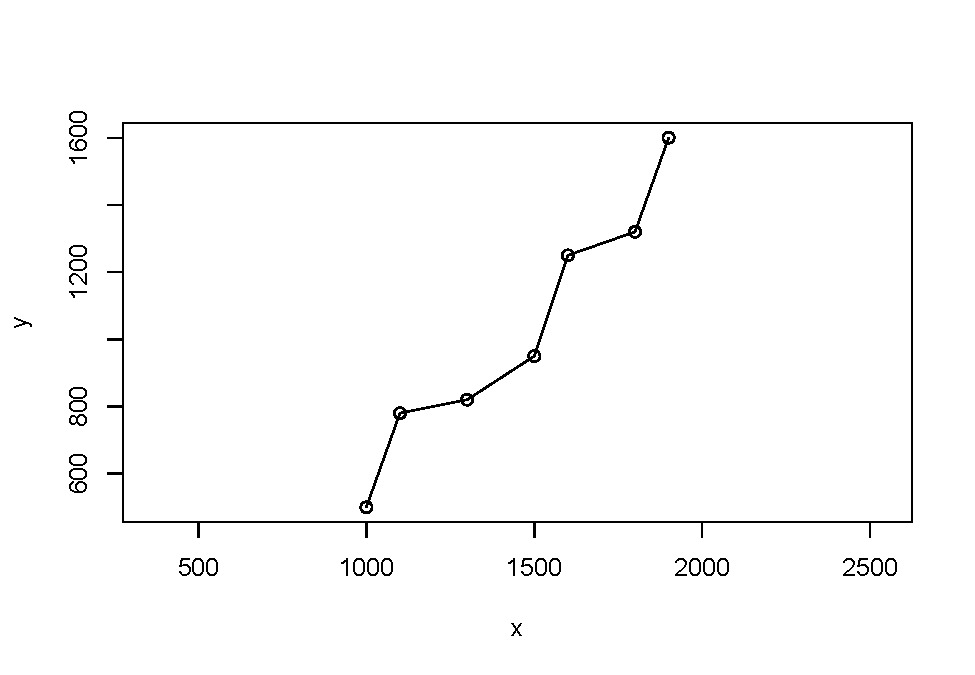
\includegraphics[width=0.75\linewidth]{EnvDataScience_files/figure-latex/introCrudeRiverMap-1} 

}

\caption{Crude river map using x y coordinates}\label{fig:introCrudeRiverMap}
\end{figure}

\begin{quote}
\textbf{Options for the \texttt{plot} function in base R}: In the visualization chapter, we'll be making use of many options in \texttt{ggplot2}, but for now we're using the \texttt{plot} function of base R, which has quite a few options that we'll introduce from time to time as needed. We'll continue to use \texttt{plot} either for a quick output of our results, or where various packages like \texttt{terra} have extended its functionality for its data types. In the above code, we used two options in plot: \texttt{asp=1} for setting the x and y scales to be the same (like on a map) with an aspect ratio of 1; and \texttt{add=TRUE} to allow the lines to be added to the same plot, using the same coordinate space.
\end{quote}

Now we'll use a loop to create a longitudinal graph by determining a cumulative longitudinal distance along the path of the river. You could look at it as straightening out the curves.

First we'll need empty vectors to populate with the longitudinal profile data:

\begin{Shaded}
\begin{Highlighting}[]
\NormalTok{d }\OtherTok{\textless{}{-}} \FunctionTok{double}\NormalTok{()      }\CommentTok{\# creates an empty numeric vector }
\NormalTok{longd }\OtherTok{\textless{}{-}} \FunctionTok{double}\NormalTok{()  }\CommentTok{\# ("double" means double{-}precision floating point)}
\NormalTok{s }\OtherTok{\textless{}{-}} \FunctionTok{double}\NormalTok{()}
\end{Highlighting}
\end{Shaded}

Then the \texttt{for} loop that goes through all of the points, but uses an \texttt{if} statement to assign an initial distance and longitudinal distance of zero, since the longitudinal profile data is just started and we don't have a distance yet.

\begin{Shaded}
\begin{Highlighting}[]
\ControlFlowTok{for}\NormalTok{(i }\ControlFlowTok{in} \DecValTok{1}\SpecialCharTok{:}\FunctionTok{length}\NormalTok{(x))\{}
  \ControlFlowTok{if}\NormalTok{(i}\SpecialCharTok{==}\DecValTok{1}\NormalTok{)\{longd[i] }\OtherTok{\textless{}{-}} \DecValTok{0}\NormalTok{; d[i] }\OtherTok{\textless{}{-}} \DecValTok{0}\NormalTok{\} }\ControlFlowTok{else}\NormalTok{ \{}
\NormalTok{    d[i] }\OtherTok{\textless{}{-}} \FunctionTok{sqrt}\NormalTok{((x[i]}\SpecialCharTok{{-}}\NormalTok{x[i}\DecValTok{{-}1}\NormalTok{])}\SpecialCharTok{\^{}}\DecValTok{2} \SpecialCharTok{+}\NormalTok{ (y[i]}\SpecialCharTok{{-}}\NormalTok{y[i}\DecValTok{{-}1}\NormalTok{])}\SpecialCharTok{\^{}}\DecValTok{2}\NormalTok{)}
\NormalTok{    longd[i] }\OtherTok{\textless{}{-}}\NormalTok{ longd[i}\DecValTok{{-}1}\NormalTok{] }\SpecialCharTok{+}\NormalTok{ d[i]}
\NormalTok{    s[i}\DecValTok{{-}1}\NormalTok{] }\OtherTok{\textless{}{-}}\NormalTok{ (elev[i]}\SpecialCharTok{{-}}\NormalTok{elev[i}\DecValTok{{-}1}\NormalTok{])}\SpecialCharTok{/}\NormalTok{d[i]}
\NormalTok{    \}}
\NormalTok{  \}}
\end{Highlighting}
\end{Shaded}

\begin{quote}
What well-known theorem is used to derive each distance? Can you find \(c^2 = a^2 + b^2\) or \(c=\sqrt{a^2+b^2}\) in the above code? Consider how Cartesian (x and y) coordinates work and where you might find a right triangle and a hypotenuse in such a coordinate system. Hint: what if \(a=\Delta{x}\) and \(b=\Delta{y}\)? Draw it out on a piece of paper to help.
\end{quote}

There is no known slope for the last point (since we have no next point), so the last slope is assigned \texttt{NA}.

\begin{Shaded}
\begin{Highlighting}[]
\NormalTok{s[}\FunctionTok{length}\NormalTok{(x)] }\OtherTok{\textless{}{-}} \ConstantTok{NA}
\end{Highlighting}
\end{Shaded}

Then we'll create a data frame out of the vectors we just built, and then display the longitudinal profile (Figure \ref{fig:introLongProfile}).

\begin{Shaded}
\begin{Highlighting}[]
\NormalTok{riverData }\OtherTok{\textless{}{-}} \FunctionTok{as.data.frame}\NormalTok{(}\FunctionTok{cbind}\NormalTok{(}\AttributeTok{x=}\NormalTok{x,}\AttributeTok{y=}\NormalTok{y,}\AttributeTok{elev=}\NormalTok{elev,}\AttributeTok{d=}\NormalTok{d,}\AttributeTok{longd=}\NormalTok{longd,}\AttributeTok{s=}\NormalTok{s))}
\NormalTok{riverData}
\end{Highlighting}
\end{Shaded}

\begin{verbatim}
##      x    y elev        d     longd           s
## 1 1000  500    0   0.0000    0.0000 0.003363364
## 2 1100  780    1 297.3214  297.3214 0.004902903
## 3 1300  820    2 203.9608  501.2822 0.012576654
## 4 1500  950    5 238.5372  739.8194 0.063245553
## 5 1600 1250   25 316.2278 1056.0471 0.235964589
## 6 1800 1320   75 211.8962 1267.9433 0.252252298
## 7 1900 1600  150 297.3214 1565.2647          NA
\end{verbatim}

\begin{Shaded}
\begin{Highlighting}[]
\FunctionTok{plot}\NormalTok{(riverData}\SpecialCharTok{$}\NormalTok{longd, riverData}\SpecialCharTok{$}\NormalTok{elev, }\AttributeTok{add=}\NormalTok{T)}
\FunctionTok{lines}\NormalTok{(riverData}\SpecialCharTok{$}\NormalTok{longd, riverData}\SpecialCharTok{$}\NormalTok{elev)}
\end{Highlighting}
\end{Shaded}

\begin{figure}

{\centering 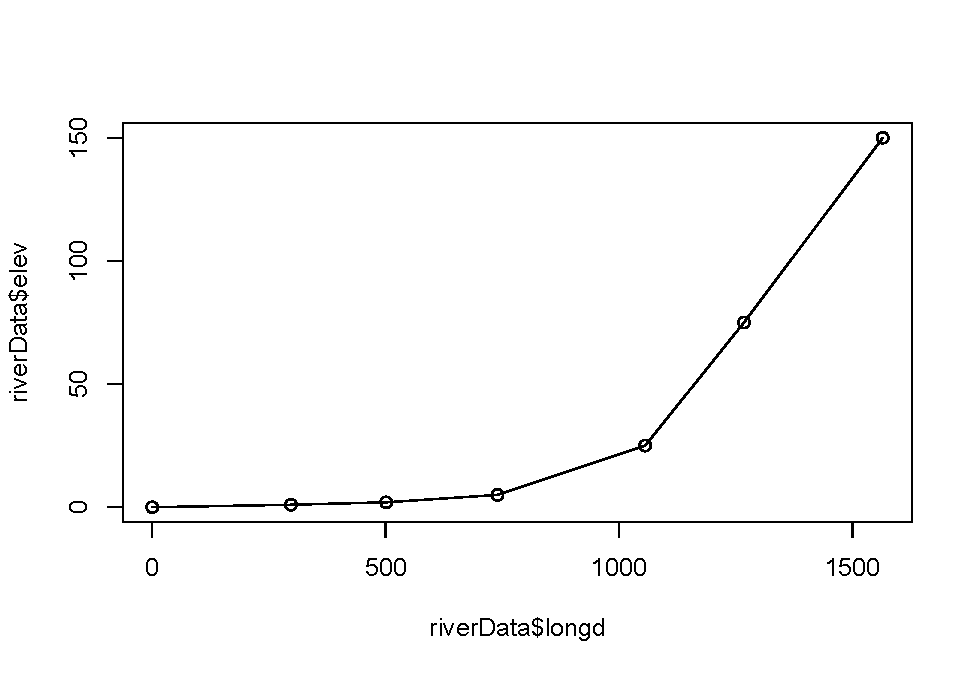
\includegraphics[width=0.75\linewidth]{EnvDataScience_files/figure-latex/introLongProfile-1} 

}

\caption{Longitudinal profile built from cumulative distances and elevation}\label{fig:introLongProfile}
\end{figure}

\subsection{Subsetting with logic}\label{subsetting-with-logic}

\index{subsetting with logic}We'll use the 2022 USDOE fuel efficiency data to list all of the car lines with at least 50 miles to the gallon. Note the creation of a Boolean logical expression with an admittedly long variable \texttt{...\ \textgreater{}=\ 50}; this will return \texttt{TRUE} or \texttt{FALSE}, so \texttt{i} will be a logical (Boolean) vector which can be used to subset a couple of variables which we'll then paste together (using vectorization of course) to create a character string vector.

\begin{Shaded}
\begin{Highlighting}[]
\FunctionTok{library}\NormalTok{(readxl)}
\NormalTok{fuelEff22 }\OtherTok{\textless{}{-}} \FunctionTok{read\_excel}\NormalTok{(}\FunctionTok{ex}\NormalTok{(}\StringTok{"USDOE\_FuelEfficiency2022.xlsx"}\NormalTok{))}
\NormalTok{i }\OtherTok{\textless{}{-}}\NormalTok{ fuelEff22}\SpecialCharTok{$}\StringTok{\textasciigrave{}}\AttributeTok{Hwy FE (Guide) {-} Conventional Fuel}\StringTok{\textasciigrave{}} \SpecialCharTok{\textgreater{}=} \DecValTok{50}
\FunctionTok{str}\NormalTok{(i)}
\end{Highlighting}
\end{Shaded}

\begin{verbatim}
##  logi [1:394] FALSE FALSE FALSE FALSE FALSE FALSE ...
\end{verbatim}

\begin{Shaded}
\begin{Highlighting}[]
\NormalTok{efficientCars }\OtherTok{\textless{}{-}} \FunctionTok{paste}\NormalTok{(fuelEff22}\SpecialCharTok{$}\NormalTok{Division[i],fuelEff22}\SpecialCharTok{$}\NormalTok{Carline[i])}
\FunctionTok{str}\NormalTok{(efficientCars)}
\end{Highlighting}
\end{Shaded}

\begin{verbatim}
##  chr [1:9] "TOYOTA COROLLA HYBRID" "HYUNDAI MOTOR COMPANY Elantra Hybrid" ...
\end{verbatim}

\begin{Shaded}
\begin{Highlighting}[]
\NormalTok{efficientCars}
\end{Highlighting}
\end{Shaded}

\begin{verbatim}
## [1] "TOYOTA COROLLA HYBRID"                    
## [2] "HYUNDAI MOTOR COMPANY Elantra Hybrid"     
## [3] "HYUNDAI MOTOR COMPANY Elantra Hybrid Blue"
## [4] "TOYOTA PRIUS"                             
## [5] "TOYOTA PRIUS Eco"                         
## [6] "HYUNDAI MOTOR COMPANY Ioniq"              
## [7] "HYUNDAI MOTOR COMPANY Ioniq Blue"         
## [8] "HYUNDAI MOTOR COMPANY Sonata Hybrid"      
## [9] "HYUNDAI MOTOR COMPANY Sonata Hybrid Blue"
\end{verbatim}

The \textbf{which} function allows us to do something similar, returning the indices of the variable or vector for which a condition \texttt{TRI87\$air\_releases\ \textgreater{}\ 1e6} is \texttt{TRUE}. Then we can use that index to do the subset.

\index{which}

\begin{Shaded}
\begin{Highlighting}[]
\FunctionTok{library}\NormalTok{(readr)}
\NormalTok{csvPath }\OtherTok{=} \FunctionTok{system.file}\NormalTok{(}\StringTok{"extdata"}\NormalTok{,}\StringTok{"TRI/TRI\_1987\_BaySites.csv"}\NormalTok{, }\AttributeTok{package=}\StringTok{"igisci"}\NormalTok{)}
\NormalTok{TRI87 }\OtherTok{\textless{}{-}} \FunctionTok{read\_csv}\NormalTok{(csvPath)}
\NormalTok{i }\OtherTok{\textless{}{-}} \FunctionTok{which}\NormalTok{(TRI87}\SpecialCharTok{$}\NormalTok{air\_releases }\SpecialCharTok{\textgreater{}} \FloatTok{1e6}\NormalTok{)}
\FunctionTok{str}\NormalTok{(i)}
\end{Highlighting}
\end{Shaded}

\begin{verbatim}
##  int [1:4] 85 96 127 328
\end{verbatim}

\begin{Shaded}
\begin{Highlighting}[]
\NormalTok{TRI87}\SpecialCharTok{$}\NormalTok{FACILITY\_NAME[i]}
\end{Highlighting}
\end{Shaded}

\begin{verbatim}
## [1] "VALERO REFINING CO-CALI FORNIA BENICIA REFINERY"
## [2] "TESLA INC"                                      
## [3] "TESORO REFINING & MARKETING CO LLC"             
## [4] "HGST INC"
\end{verbatim}

The \textbf{\%in\%} operator is very useful when we have very specific items to select.
\index{in}

\begin{Shaded}
\begin{Highlighting}[]
\FunctionTok{library}\NormalTok{(readr)}
\NormalTok{csvPath }\OtherTok{=} \FunctionTok{system.file}\NormalTok{(}\StringTok{"extdata"}\NormalTok{,}\StringTok{"TRI/TRI\_1987\_BaySites.csv"}\NormalTok{, }\AttributeTok{package=}\StringTok{"igisci"}\NormalTok{)}
\NormalTok{TRI87 }\OtherTok{\textless{}{-}} \FunctionTok{read\_csv}\NormalTok{(csvPath)}
\NormalTok{i }\OtherTok{\textless{}{-}}\NormalTok{ TRI87}\SpecialCharTok{$}\NormalTok{COUNTY }\SpecialCharTok{\%in\%} \FunctionTok{c}\NormalTok{(}\StringTok{"NAPA"}\NormalTok{,}\StringTok{"SONOMA"}\NormalTok{)}
\NormalTok{TRI87}\SpecialCharTok{$}\NormalTok{FACILITY\_NAME[i]}
\end{Highlighting}
\end{Shaded}

\begin{verbatim}
## [1] "SAWYER OF NAPA"                               
## [2] "BERINGER VINEYARDS"                           
## [3] "CAL-WOOD DOOR INC"                            
## [4] "SOLA OPTICAL USA INC"                         
## [5] "KEYSIGHT TECHNOLOGIES INC"                    
## [6] "SANTA ROSA STAINLESS STEEL"                   
## [7] "OPTICAL COATING LABORATORY INC"               
## [8] "MGM BRAKES"                                   
## [9] "SEBASTIANI VINEYARDS INC, SONOMA CASK CELLARS"
\end{verbatim}

\subsection{Apply functions}\label{apply}

There are many \index{apply functions}apply functions in R, and they often obviate the need for looping. For instance:

\begin{itemize}
\tightlist
\item
  \texttt{apply} derives values at margins of rows and columns, e.g.~to sum across rows or down columns.
\end{itemize}

\begin{Shaded}
\begin{Highlighting}[]
\CommentTok{\# matrix apply – the same would apply to data frames}
\NormalTok{matrix12 }\OtherTok{\textless{}{-}} \DecValTok{1}\SpecialCharTok{:}\DecValTok{12}
\FunctionTok{dim}\NormalTok{(matrix12) }\OtherTok{\textless{}{-}} \FunctionTok{c}\NormalTok{(}\DecValTok{3}\NormalTok{,}\DecValTok{4}\NormalTok{)}
\NormalTok{rowsums }\OtherTok{\textless{}{-}} \FunctionTok{apply}\NormalTok{(matrix12, }\DecValTok{1}\NormalTok{, sum)}
\NormalTok{colsums }\OtherTok{\textless{}{-}} \FunctionTok{apply}\NormalTok{(matrix12, }\DecValTok{2}\NormalTok{, sum)}
\FunctionTok{sum}\NormalTok{(rowsums)}
\end{Highlighting}
\end{Shaded}

\begin{verbatim}
## [1] 78
\end{verbatim}

\begin{Shaded}
\begin{Highlighting}[]
\FunctionTok{sum}\NormalTok{(colsums)}
\end{Highlighting}
\end{Shaded}

\begin{verbatim}
## [1] 78
\end{verbatim}

\begin{Shaded}
\begin{Highlighting}[]
\NormalTok{zero }\OtherTok{\textless{}{-}} \FunctionTok{sum}\NormalTok{(rowsums) }\SpecialCharTok{{-}} \FunctionTok{sum}\NormalTok{(colsums)}
\NormalTok{matrix12}
\end{Highlighting}
\end{Shaded}

\begin{verbatim}
##      [,1] [,2] [,3] [,4]
## [1,]    1    4    7   10
## [2,]    2    5    8   11
## [3,]    3    6    9   12
\end{verbatim}

Apply functions satisfy one of the needs that spreadsheets are used for. Consider how often you use sum, mean, or similar functions in Excel.

\textbf{\texttt{sapply}}

\index{sapply}sapply applies functions to either:

\begin{itemize}
\tightlist
\item
  all elements of a vector -- unary functions only
\end{itemize}

\begin{Shaded}
\begin{Highlighting}[]
\FunctionTok{sapply}\NormalTok{(}\DecValTok{1}\SpecialCharTok{:}\DecValTok{12}\NormalTok{, sqrt)}
\end{Highlighting}
\end{Shaded}

\begin{verbatim}
##  [1] 1.000000 1.414214 1.732051 2.000000 2.236068 2.449490 2.645751 2.828427
##  [9] 3.000000 3.162278 3.316625 3.464102
\end{verbatim}

\begin{itemize}
\tightlist
\item
  or all variables of a data frame (not a matrix), where it works much like a column-based apply (since variables are columns) but more easily interpreted without the need of specifying columns with 2:
\end{itemize}

\begin{Shaded}
\begin{Highlighting}[]
\FunctionTok{sapply}\NormalTok{(cars,mean)  }\CommentTok{\# same as apply(cars,2,mean)}
\end{Highlighting}
\end{Shaded}

\begin{verbatim}
## speed  dist 
## 15.40 42.98
\end{verbatim}

\begin{Shaded}
\begin{Highlighting}[]
\NormalTok{temp02 }\OtherTok{\textless{}{-}} \FunctionTok{c}\NormalTok{(}\FloatTok{10.7}\NormalTok{,}\FloatTok{9.7}\NormalTok{,}\FloatTok{7.7}\NormalTok{,}\FloatTok{9.2}\NormalTok{,}\FloatTok{7.3}\NormalTok{,}\FloatTok{6.7}\NormalTok{,}\FloatTok{4.0}\NormalTok{,}\FloatTok{5.0}\NormalTok{,}\FloatTok{0.9}\NormalTok{,}\SpecialCharTok{{-}}\FloatTok{1.1}\NormalTok{,}\SpecialCharTok{{-}}\FloatTok{0.8}\NormalTok{,}\SpecialCharTok{{-}}\FloatTok{4.4}\NormalTok{)}
\NormalTok{temp03 }\OtherTok{\textless{}{-}} \FunctionTok{c}\NormalTok{(}\FloatTok{13.1}\NormalTok{,}\FloatTok{11.4}\NormalTok{,}\FloatTok{9.4}\NormalTok{,}\FloatTok{10.9}\NormalTok{,}\FloatTok{8.9}\NormalTok{,}\FloatTok{8.4}\NormalTok{,}\FloatTok{6.7}\NormalTok{,}\FloatTok{7.6}\NormalTok{,}\FloatTok{2.8}\NormalTok{,}\FloatTok{1.6}\NormalTok{,}\FloatTok{1.2}\NormalTok{,}\SpecialCharTok{{-}}\FloatTok{2.1}\NormalTok{)}
\FunctionTok{sapply}\NormalTok{(}\FunctionTok{as.data.frame}\NormalTok{(}\FunctionTok{cbind}\NormalTok{(temp02,temp03)),mean) }\CommentTok{\# has to be a data frame}
\end{Highlighting}
\end{Shaded}

\begin{verbatim}
##   temp02   temp03 
## 4.575000 6.658333
\end{verbatim}

While various \texttt{apply} functions are in base R, the purrr package takes these further. See \url{https://www.rstudio.com/resources/cheatsheets/} for more information on this and other packages in the RStudio/tidyverse world.

\section{RStudio projects}\label{rstudio}

\index{RStudio projects}So far, you've been using RStudio, and it organizes your code and data into a project folder. You should familiarize yourself with where things are being saved and where you can find things. Start by seeing your \emph{working directory} with \index{getwd}:

\begin{verbatim}
getwd()
\end{verbatim}

When you create a new RStudio project with \texttt{File/New\ Project...}, it will set the working directory to the \emph{project folder}, where you create the project. (You can change the working directory with \texttt{setwd()} but I don't recommend it.) The project folder is useful for keeping things organized and allowing you to use relative paths to your data and allow everything to be moved somewhere else and still work. The project file has the extension \texttt{.Rproj} and it will reside in the project folder. If you've saved any scripts (\texttt{.R})or R Markdown (\texttt{.Rmd}) documents, they'll also reside in the project folder; and if you've saved any data, or if you want to read any data without providing the full path or using the \texttt{extdata} access method, those data files (e.g.~\texttt{.csv}) will be in that project folder. You can see your scripts, R Markdown documents, and data files using the Files tab in the default lower right pane of RStudio.

\textbf{RStudio projects} are going to be the way we'll want to work for the rest of this book, so you'll often want to create new ones for particular data sets so things don't get messy. And you may want to create data folders within your project folder, as we have in the \texttt{igisci} extdata folder, to keep things organized. Since we're using our \texttt{igisci} package, this is less of an issue since at least input data isn't stored in the project folder. However you're going to be creating data, so you'll want to manage your data in individual projects. You may want to start a new project for each data set, using File/New Project, and try to keep things organized (things can get messy fast!)

\textbf{Just opening an \texttt{.Rmd\ file} from your computer will not set the working directory to the folder you're in, even if it's a project folder.} It will instead open the document within the most recent project you've been working in. You will find that you don't have simple relative access to any data in your folder. Instead, you need to open the project!

In this book, we'll be making a lot of use of data provided for you from various data packages such as built-in data, \texttt{palmerpenguins} (\citeproc{ref-palmer}{Horst et al. 2020}), or \texttt{igisci}, but they correspond to specific research projects, such as Sierra Climate to which several data frames and spatial data apply. For this chapter, you can probably just use one project, but later you'll find it useful to create separate projects for each data set -- \emph{such as a} \textbf{\texttt{sierra}} \emph{project} and return to it every time it applies.

In that project, you'll build a series of scripts, many of which you'll re-use to develop new methods. When you're working on your own project with your own data files, you should store these in a \textbf{\texttt{data}} folder inside the project folder. With the project folder as the default working directory, you can use \index{relative paths}\emph{relative paths}, and everything will work even if the project folder is moved. So, for instance, you can specify \textbf{\texttt{"data/mydata.csv"}} \emph{as the path} to a csv of that name. You can still access package data, including extdata folders and files, but your processed and saved or imported data will reside with your project.

An \index{absolute paths}\emph{absolute path} to somewhere on your computer in contrast won't work for anyone else trying to run your code; absolute paths should only be used for servers that other users have access to and URLs on the web.

\subsection{R Markdown}\label{rmarkdown}

An alternative to writing scripts is writing \index{R Markdown}\emph{R Markdown} documents, which includes both formatted text (such as you're seeing in this book, like \emph{italics} created using asterisks) and code chunks. R lends itself to running code in chunks, as opposed to creating complete tools that run all of the way through. This book is built from R Markdown documents organized in a bookdown structure, and most of the figures are created from R code chunks. There are also many good resources on writing R Markdown documents, including the very thorough \emph{R Markdown: The Definitive Guide} (\citeproc{ref-RMarkdown}{Xie et al. 2019}).

\pagebreak

\section{Exercises: Introduction to R}\label{exercises-introduction-to-r}

\begin{exercise}
Assign scalars for your name, city, state and zip code, and use \texttt{paste()} to combine them, and assign them to the object \texttt{me}. What is the class of \texttt{me}?
\end{exercise}

\begin{exercise}
Knowing that trigonometric functions require angles (including azimuth directions) to be provided in radians, and that degrees can be converted into radians by dividing by 180 and multiplying that by pi, derive the sine of 30 degrees with an R expression. (Base R knows what pi is, so you can just use \texttt{pi}.)
\end{exercise}

\begin{exercise}
If two sides of a right triangle on a map can be represented as \(dX\) and \(dY\) and the direct line path between them \(c\), and the coordinates of two points on a map might be given as \((x1,y1)\) and \((x2,y2)\), with \(dX=x2-x1\) and \(dY=y2-y1\), use the Pythagorean theorem to derive the distance between them and assign that expression to \(c\). Start by assigning the input scalars.
\end{exercise}

\begin{exercise}
You can create a vector uniform random numbers from 0 to 1 using \texttt{runif(n=30)} where n=30 says to make 30 of them. Use the \texttt{round()} function to round \emph{each} of the values (it vectorizes them), and provide what you created and explain what happened.
\end{exercise}

\begin{exercise}
Create two vectors \texttt{x} and \texttt{y} of 10 numbers each with the c() function, then assigning to x and y. Then plot(x,y), and provide the three lines of code you used to do the assignment and plot.
\end{exercise}

\begin{exercise}
Change your code from the previous question so that one value is NA (entered simply as \texttt{NA}, no quotation marks), and derive the mean value for x. Then add \texttt{,na.rm=T} to the parameters for \texttt{mean()}. Also do this for y. Describe your results and explain what happens.
\end{exercise}

\begin{exercise}
Create two sequences, \texttt{a} and \texttt{b}, with \texttt{a} all odd numbers from 1 to 99, \texttt{b} all even numbers from 2 to 100. Then derive c through vector division of \texttt{b/a}. Plot a and c together as a scatterplot.
\end{exercise}

\begin{exercise}
Referring to the \textbf{Matrices} section, create the same \texttt{sierradata} matrix using the same data vectors repeated here \ldots{}

\ldots{} then convert it to a data frame (using the same \texttt{sierradata} object name), and \emph{from that data frame} plot temperature (\texttt{tC}) against latitude (\texttt{lat}).
\end{exercise}

\begin{exercise}
From that \texttt{sierradata} data frame, derive colmeans using the \texttt{mean} parameter on the columns \texttt{2} for \texttt{apply()}.
\end{exercise}

\begin{exercise}
Do the same thing with the sierra data frame with \texttt{sapply()}.
\end{exercise}

\chapter{Data Abstraction}\label{abstraction}

Abstracting data from large data sets (or even small ones) is critical
to data science. The most common first step to visualization is
abstracting the data in a form that allows for the visualization goal in
mind. If you've ever worked with data in spreadsheets, you commonly will
be faced with some kind of data manipulation to create meaningful
graphs, unless that spreadsheet is specifically designed for it, but
then doing something else with the data is going to require some work.

\begin{figure}

{\centering 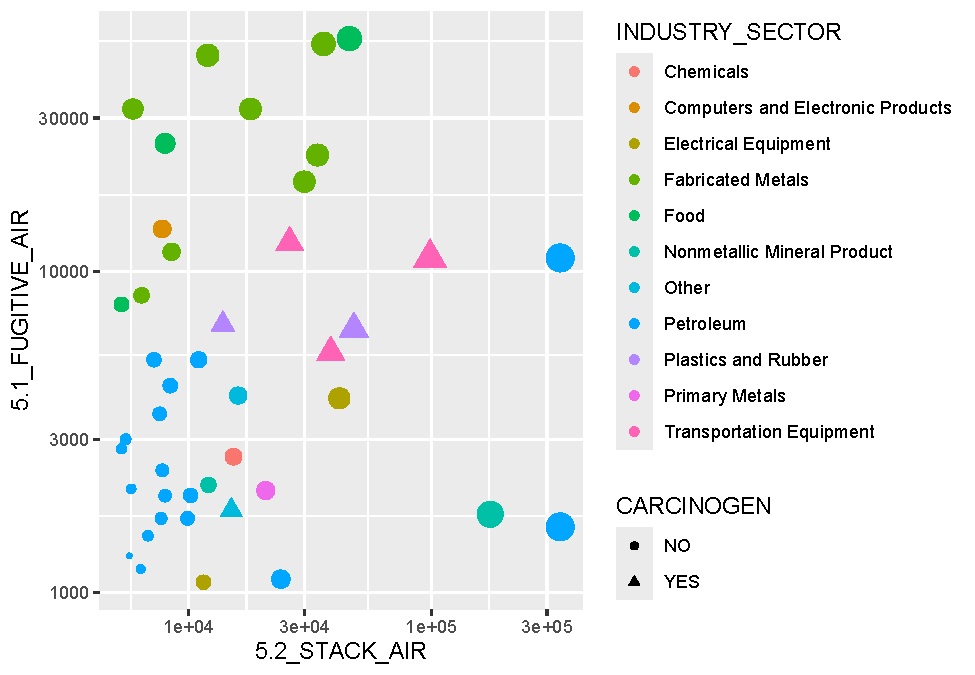
\includegraphics[width=0.75\linewidth]{EnvDataScience_files/figure-latex/Abstraction-1} 

}

\caption{Visualization of some abstracted data from the EPA Toxic Release Inventory}\label{fig:Abstraction}
\end{figure}

Figure \ref{fig:Abstraction} started with abstracting some data from
EPA's Toxic Release Inventory (TRI) program, which holds data reported
from a large number of facilities that must report either ``stack'' or
``fugitive'' air. Some of the abstraction had already happened when I used
the EPA website to download data for particular years and only in
California. But there's more we need to do, and we'll want to use some
\texttt{dplyr} functions to help with it.

At this point, we've learned the basics of working with the R language.
From here we'll want to explore how to analyze data, statistically,
spatially, and temporally. One part of this is abstracting information
from existing data sets by selecting variables and observations and
summarizing their statistics.

In the previous chapter, we learned some abstraction methods in base R,
such as selecting parts of data frames and applying some functions
across the data frame. There's a lot we can do with these methods, and
they continue to be developed and improved. We'll continue to use them,
but they can employ some fairly arcane language. There are many packages
that extend R's functionality, but some of the most important for data
science can be found in the various packages of ``The Tidyverse''
(\citeproc{ref-wickham2016r}{Wickham and Grolemund 2016}), which has the philosophy of making data manipulation
more intuitive.

We'll start with \index{dplyr}\textbf{\texttt{dplyr}}, which includes an array of
data manipulation tools, including \textbf{\texttt{select}} for selecting variables,
\textbf{\texttt{filter}} for subsetting observations, \textbf{\texttt{summarize}} for reducing
variables to summary statistics, typically stratified by groups, and
\textbf{\texttt{mutate}} for creating new variables from mathematical expressions
from existing variables. Some \texttt{dplyr} tools such as data joins we'll
look at later in the data transformation chapter.

\section{The Tidyverse}\label{tidyverse}

The \index{tidyverse}tidyverse refers to a suite of R packages developed
at RStudio (now \emph{posit}) (see \url{https://posit.co} and
\href{https://r4ds.had.co.nz}{\textless https://r4ds.had.co.nz\textgreater{}}) for
facilitating data processing and analysis. While R itself is designed
around exploratory data analysis, the tidyverse takes it further. Some
of the packages in the tidyverse that are widely used are:

\begin{itemize}
\tightlist
\item
  \textbf{\texttt{dplyr}} : \index{dplyr}data manipulation like a database
\item
  \textbf{\texttt{readr}} : \index{readr}better methods for reading and writing
  rectangular data
\item
  \textbf{\texttt{tidyr}} : \index{tidyr}reorganization methods that extend
  dplyr's database capabilities
\item
  \textbf{\texttt{purrr}} : \index{purrr}expanded programming toolkit including
  enhanced ``apply'' methods
\item
  \textbf{\texttt{tibble}} : \index{tibble}improved data frame
\item
  \textbf{\texttt{stringr}} : \index{stringr}string manipulation library
\item
  \textbf{\texttt{ggplot2}} : \index{ggplot2}graphing system based on \emph{the grammar
  of graphics}
\end{itemize}

In this chapter, we'll be mostly exploring \textbf{dplyr}, with a few other
things thrown in like reading data frames with \textbf{readr}; and we'll also
introduce a few other base R methods. For simplicity, we can just
include \texttt{library(tidyverse)} to get everything, and of course the base R
methods are already there.

\section{Tibbles}\label{tibbles}

\index{tibble}Tibbles are an improved type of data frame

\begin{itemize}
\tightlist
\item
  part of the tidyverse
\item
  serve the same purpose as a data frame, and all data frame
  operations work
\end{itemize}

Advantages

\begin{itemize}
\tightlist
\item
  display better
\item
  can be composed of more complex objects like lists, etc.
\item
  can be grouped
\end{itemize}

There multiple ways to create a tibble:

\begin{itemize}
\tightlist
\item
  Reading from a CSV using \texttt{read\_csv()}. \emph{Note the underscore, a
  function naming convention in the tidyverse.}
\item
  Using \texttt{tibble()} to either build from vectors or from scratch, or
  convert from a different type of data frame.
\item
  Using \texttt{tribble()} to build in code from scratch.
\item
  Using various tidyverse functions that return tibbles.
\end{itemize}

\subsection{Building a tibble from vectors}\label{building-a-tibble-from-vectors}

We'll start by looking at a couple of built-in
\index{character vectors}character vectors (there are lots of things
like this in R):

\begin{itemize}
\tightlist
\item
  \texttt{letters} : lowercase letters
\item
  \texttt{LETTERS} : uppercase letters
\end{itemize}

\begin{Shaded}
\begin{Highlighting}[]
\NormalTok{letters}
\end{Highlighting}
\end{Shaded}

\begin{verbatim}
##  [1] "a" "b" "c" "d" "e" "f" "g" "h" "i" "j" "k" "l" "m" "n" "o" "p" "q" "r" "s"
## [20] "t" "u" "v" "w" "x" "y" "z"
\end{verbatim}

\begin{Shaded}
\begin{Highlighting}[]
\NormalTok{LETTERS}
\end{Highlighting}
\end{Shaded}

\begin{verbatim}
##  [1] "A" "B" "C" "D" "E" "F" "G" "H" "I" "J" "K" "L" "M" "N" "O" "P" "Q" "R" "S"
## [20] "T" "U" "V" "W" "X" "Y" "Z"
\end{verbatim}

\ldots{} then make a tibble of \texttt{letters}, \texttt{LETTERS}, and two random sets of
26 values, one \index{rnorm}normally distributed, the other
\index{runif}uniform:

\begin{Shaded}
\begin{Highlighting}[]
\NormalTok{norm }\OtherTok{\textless{}{-}} \FunctionTok{rnorm}\NormalTok{(}\DecValTok{26}\NormalTok{)}
\NormalTok{unif }\OtherTok{\textless{}{-}} \FunctionTok{runif}\NormalTok{(}\DecValTok{26}\NormalTok{)}
\FunctionTok{library}\NormalTok{(tidyverse)}
\NormalTok{tibble26 }\OtherTok{\textless{}{-}} \FunctionTok{tibble}\NormalTok{(letters,LETTERS,norm,unif)}
\NormalTok{tibble26}
\end{Highlighting}
\end{Shaded}

\begin{verbatim}
## # A tibble: 26 x 4
##    letters LETTERS    norm   unif
##    <chr>   <chr>     <dbl>  <dbl>
##  1 a       A        0.245  0.893 
##  2 b       B        0.0101 0.500 
##  3 c       C        1.61   0.268 
##  4 d       D        0.0788 0.360 
##  5 e       E        0.504  0.764 
##  6 f       F        0.268  0.0504
##  7 g       G       -1.21   0.332 
##  8 h       H       -0.894  0.720 
##  9 i       I        0.922  0.941 
## 10 j       J       -0.0222 0.0566
## # i 16 more rows
\end{verbatim}

\begin{quote}
See section \ref{random} for more on creating random (or rather
\emph{pseudo-random}) numbers in R.
\end{quote}

\subsubsection{Combining built-in data of various types}\label{combining-built-in-data-of-various-types}

As we're starting to see, there are a lot of data sets that are built
into base R. They tend to be fairly simple structures like vectors and
time series, shown as ``Values'' in the Environment tab of RStudio. But we
might want to combine them into tibbles to make them more useful.

Have a look at the various data sets that together form data from the 50
United States: character vectors \texttt{state.name} and \texttt{state.abb}, factors
\texttt{state.region}, and a \texttt{state.x77} matrix.

\begin{quote}
Use ?state to learn more about this data
\end{quote}

You'll find that they each have a length of 50, and they happen to be in
the same order by state. That will make it easy to combine them. Note in
the following code that we provide better names for the vectors, but use
\texttt{as\_tibble} to get all of the variables, with their names, from the
matrix \texttt{state.x77}.

\begin{Shaded}
\begin{Highlighting}[]
\NormalTok{st }\OtherTok{\textless{}{-}} \FunctionTok{bind\_cols}\NormalTok{(}\AttributeTok{Name=}\NormalTok{state.name, }\AttributeTok{Abb=}\NormalTok{state.abb, }\AttributeTok{Region=}\NormalTok{state.region, }\FunctionTok{as\_tibble}\NormalTok{(state.x77))}
\FunctionTok{head}\NormalTok{(st)}
\end{Highlighting}
\end{Shaded}

\begin{verbatim}
## # A tibble: 6 x 11
##   Name     Abb   Region Population Income Illiteracy `Life Exp` Murder `HS Grad`
##   <chr>    <chr> <fct>       <dbl>  <dbl>      <dbl>      <dbl>  <dbl>     <dbl>
## 1 Alabama  AL    South        3615   3624        2.1       69.0   15.1      41.3
## 2 Alaska   AK    West          365   6315        1.5       69.3   11.3      66.7
## 3 Arizona  AZ    West         2212   4530        1.8       70.6    7.8      58.1
## 4 Arkansas AR    South        2110   3378        1.9       70.7   10.1      39.9
## 5 Califor~ CA    West        21198   5114        1.1       71.7   10.3      62.6
## 6 Colorado CO    West         2541   4884        0.7       72.1    6.8      63.9
## # i 2 more variables: Frost <dbl>, Area <dbl>
\end{verbatim}

\begin{quote}
Use the methods you've learned in RStudio to see what this tibble
contains, and note that not all variables are displayed in the simple
\texttt{head()} output above. Can you find \texttt{Frost}, the ``mean number of days
with minimum temperature below freezing (1931-1960) in capital or
large city''? Those would probably be fewer now.
\end{quote}

\subsection{tribble}\label{tribble}

\emph{As long as you don't let them multiply in your starship},
\index{tribble}tribbles are handy for creating tibbles. (Or rather the
\texttt{tribble} function is a handy way to create tibbles in code.) You simply
create the variable names with a series of entries starting with a
tilde, then the data is entered one row at a time. If you line them all
up in your code one row at a time, it's easy to enter the data
accurately (Table \ref{tab:tribble}).

\begin{Shaded}
\begin{Highlighting}[]
\NormalTok{peaks }\OtherTok{\textless{}{-}} \FunctionTok{tribble}\NormalTok{(}
  \SpecialCharTok{\textasciitilde{}}\NormalTok{peak, }\SpecialCharTok{\textasciitilde{}}\NormalTok{elev, }\SpecialCharTok{\textasciitilde{}}\NormalTok{longitude, }\SpecialCharTok{\textasciitilde{}}\NormalTok{latitude,}
  \StringTok{"Mt. Whitney"}\NormalTok{, }\DecValTok{4421}\NormalTok{, }\SpecialCharTok{{-}}\FloatTok{118.2}\NormalTok{, }\FloatTok{36.5}\NormalTok{,}
  \StringTok{"Mt. Elbert"}\NormalTok{, }\DecValTok{4401}\NormalTok{, }\SpecialCharTok{{-}}\FloatTok{106.4}\NormalTok{, }\FloatTok{39.1}\NormalTok{,}
  \StringTok{"Mt. Hood"}\NormalTok{, }\DecValTok{3428}\NormalTok{, }\SpecialCharTok{{-}}\FloatTok{121.7}\NormalTok{, }\FloatTok{45.4}\NormalTok{,}
  \StringTok{"Mt. Rainier"}\NormalTok{, }\DecValTok{4392}\NormalTok{, }\SpecialCharTok{{-}}\FloatTok{121.8}\NormalTok{, }\FloatTok{46.9}\NormalTok{)}
\NormalTok{knitr}\SpecialCharTok{::}\FunctionTok{kable}\NormalTok{(peaks, }\AttributeTok{caption =} \StringTok{\textquotesingle{}Peaks tibble\textquotesingle{}}\NormalTok{)}
\end{Highlighting}
\end{Shaded}

\begin{table}

\caption{\label{tab:tribble}Peaks tibble}
\centering
\begin{tabular}[t]{l|r|r|r}
\hline
peak & elev & longitude & latitude\\
\hline
Mt. Whitney & 4421 & -118.2 & 36.5\\
\hline
Mt. Elbert & 4401 & -106.4 & 39.1\\
\hline
Mt. Hood & 3428 & -121.7 & 45.4\\
\hline
Mt. Rainier & 4392 & -121.8 & 46.9\\
\hline
\end{tabular}
\end{table}

\subsection{read\_csv}\label{csv}

The \index{read csv}\texttt{read\_csv} function does somewhat the same thing as
\texttt{read.csv} in base R, but creates a tibble instead of a data.frame, and
has some other properties we'll look at below.\index{igisci package}

\begin{quote}
Note that the code below accesses data we'll be using a lot, from EPA
Toxic Release Inventory (TRI) data. If you want to keep this data
organized in a separate project, you might consider creating a new
\textbf{\texttt{air\_quality}} project. This is optional, and you can get by with
staying in one project since all of our data will be accessed from the
\texttt{igisci} package. But in your own work, you will find it useful to
create separate projects to keep things organized with your code and
data together.
\end{quote}

\begin{Shaded}
\begin{Highlighting}[]
\FunctionTok{library}\NormalTok{(tidyverse); }\FunctionTok{library}\NormalTok{(igisci)}
\NormalTok{TRI87 }\OtherTok{\textless{}{-}} \FunctionTok{read\_csv}\NormalTok{(}\FunctionTok{ex}\NormalTok{(}\StringTok{"TRI/TRI\_1987\_BaySites.csv"}\NormalTok{))}
\NormalTok{TRI87df }\OtherTok{\textless{}{-}} \FunctionTok{read.csv}\NormalTok{(}\FunctionTok{ex}\NormalTok{(}\StringTok{"TRI/TRI\_1987\_BaySites.csv"}\NormalTok{))}
\NormalTok{TRI87b }\OtherTok{\textless{}{-}} \FunctionTok{tibble}\NormalTok{(TRI87df)}
\FunctionTok{identical}\NormalTok{(TRI87, TRI87b)}
\end{Highlighting}
\end{Shaded}

\begin{verbatim}
## [1] FALSE
\end{verbatim}

Note that they're not identical. \emph{So what's the difference between}
\index{read\_csv}\texttt{read\_csv} and \index{read.csv}\texttt{read.csv}? Why would we
use one over the other? Since their names are so similar, you may
accidentally choose one or the other. Some things to consider:

\begin{itemize}
\tightlist
\item
  To use read\_csv, you need to load the \texttt{readr} or \texttt{tidyverse}
  library, or use \texttt{readr::read\_csv}.
\item
  The \texttt{read.csv} function ``fixes'' some things and sometimes that might
  be desired: problematic variable names like \texttt{MLY-TAVG-NORMAL} become
  \texttt{MLY.TAVG.NORMAL} -- but this may create problems if those original
  names are a standard designation.
\item
  With \texttt{read.csv}, numbers stored as characters are converted to
  numbers: ``01'' becomes 1, ``02'' becomes 2, etc.
\item
  There are other known problems that read\_csv avoids.
\end{itemize}

\textbf{Recommendation}: Use \texttt{read\_csv} and \texttt{write\_csv}.

\begin{quote}
You can still just call tibbles ``data frames'', since they are still
data frames, and in this book we'll follow that practice.
\end{quote}

\section{Summarizing variable distributions}\label{summarizing-variable-distributions}

A simple \index{statistical summary}statistical summary is very easy to
do in R, and we'll use \index{eucoak data}\textbf{\texttt{eucoak}} data in the
\texttt{igisci} package from a study of comparative runoff and erosion under
eucalyptus and oak canopies (\citeproc{ref-eucoak}{Thompson et al. 2016}). In this study (Figure
\ref{fig:absEucOakStudy}), we looked at the amount of runoff and
erosion captured in Gerlach troughs on paired eucalyptus and oak sites
in the San Francisco Bay Area. \emph{You might consider creating a \texttt{eucoak}
project, since we'll be referencing this data set in several places.}



\begin{figure}

{\centering 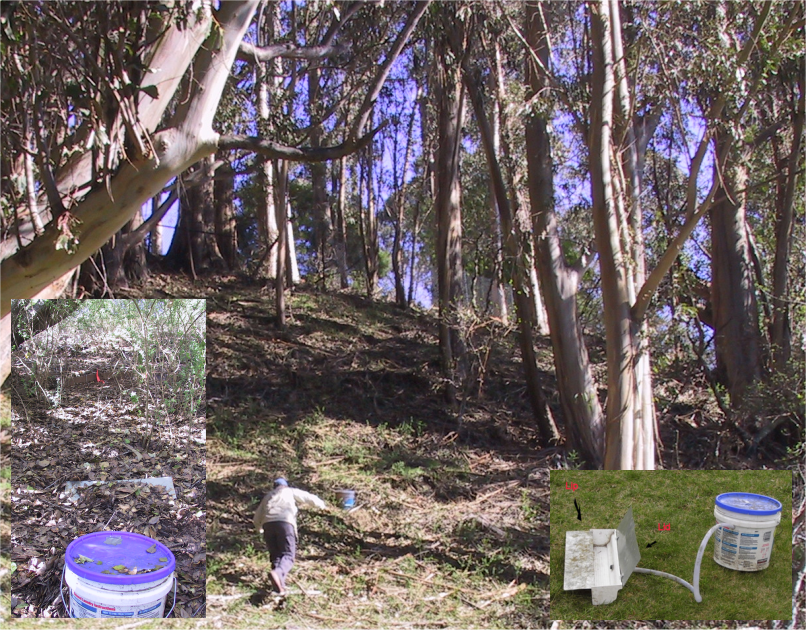
\includegraphics[width=0.75\linewidth]{img/eucoak} 

}

\caption{Euc-Oak paired plot runoff and erosion study (Thompson et al. (\citeproc{ref-eucoak}{2016}))}\label{fig:absEucOakStudy}
\end{figure}

\begin{Shaded}
\begin{Highlighting}[]
\FunctionTok{library}\NormalTok{(igisci)}
\FunctionTok{summary}\NormalTok{(eucoakrainfallrunoffTDR)}
\end{Highlighting}
\end{Shaded}

\begin{verbatim}
##         site        site #             date          month       rain_mm     
##  Length   :90   Min.   :1.000   Length   :90   Length   :90   Min.   : 1.00  
##  N.unique : 8   1st Qu.:2.000   N.unique :25   N.unique : 7   1st Qu.:16.00  
##  N.blank  : 0   Median :4.000   N.blank  : 0   N.blank  : 0   Median :28.50  
##  Min.nchar: 3   Mean   :4.422   Min.nchar: 8   Min.nchar: 8   Mean   :37.99  
##  Max.nchar: 3   3rd Qu.:6.000   Max.nchar:10   Max.nchar: 9   3rd Qu.:63.25  
##                 Max.   :8.000                                 Max.   :99.00  
##                                                               NAs    :18     
##     rain_oak        rain_euc      runoffL_oak      runoffL_euc   
##  Min.   : 1.00   Min.   : 1.00   Min.   : 0.000   Min.   : 0.00  
##  1st Qu.:16.00   1st Qu.:14.75   1st Qu.: 0.000   1st Qu.: 0.07  
##  Median :30.50   Median :30.00   Median : 0.450   Median : 1.20  
##  Mean   :35.08   Mean   :34.60   Mean   : 2.032   Mean   : 2.45  
##  3rd Qu.:50.50   3rd Qu.:50.00   3rd Qu.: 2.800   3rd Qu.: 3.30  
##  Max.   :98.00   Max.   :96.00   Max.   :14.000   Max.   :16.00  
##  NAs    :2       NAs    :2       NAs    :5        NAs    :3      
##    slope_oak       slope_euc       aspect_oak      aspect_euc   
##  Min.   : 9.00   Min.   : 9.00   Min.   :100.0   Min.   :106.0  
##  1st Qu.:12.00   1st Qu.:12.00   1st Qu.:143.0   1st Qu.:175.0  
##  Median :24.50   Median :23.00   Median :189.0   Median :196.5  
##  Mean   :21.62   Mean   :19.34   Mean   :181.9   Mean   :191.2  
##  3rd Qu.:30.50   3rd Qu.:25.00   3rd Qu.:220.0   3rd Qu.:224.0  
##  Max.   :32.00   Max.   :31.00   Max.   :264.0   Max.   :296.0  
##                                                                 
##  surface_tension_oak surface_tension_euc runoff_rainfall_ratio_oak
##  Min.   :37.40       Min.   :28.51       Min.   :0.00000          
##  1st Qu.:72.75       1st Qu.:32.79       1st Qu.:0.00000          
##  Median :72.75       Median :37.40       Median :0.02045          
##  Mean   :68.35       Mean   :43.11       Mean   :0.05358          
##  3rd Qu.:72.75       3rd Qu.:56.41       3rd Qu.:0.08485          
##  Max.   :72.75       Max.   :72.75       Max.   :0.42000          
##  NAs    :22          NAs    :22          NAs    :5                
##  runoff_rainfall_ratio_euc
##  Min.   :0.000000         
##  1st Qu.:0.003027         
##  Median :0.047619         
##  Mean   :0.065902         
##  3rd Qu.:0.083603         
##  Max.   :0.335652         
##  NAs    :3
\end{verbatim}

In the summary output, how are character variables handled differently
from numeric ones?

Remembering what we discussed in the previous chapter, consider the
\texttt{site} variable (Figure \ref{fig:absEucOakSites}), and in particular
its Length. Looking at the table, what does that length represent?

There are a couple of ways of removing duplicates from a data frame,
such as the \texttt{unique()}\index{unique} and the similar
\texttt{dplyr::distinct()}\index{distinct} functions. In the Transformation
chapter, we'll use this as one step in paring down big data from
groundwater wells.

We could also use \texttt{unique()} to simply have a quick look at our list of
subcanopy runoff measurement sites, which helps us consider using \texttt{site}
as a factor for statistical analysis. Consider what these return:

\begin{Shaded}
\begin{Highlighting}[]
\FunctionTok{unique}\NormalTok{(eucoakrainfallrunoffTDR}\SpecialCharTok{$}\NormalTok{site)}
\end{Highlighting}
\end{Shaded}

\begin{verbatim}
## [1] "AB1" "AB2" "KM1" "PR1" "TP1" "TP2" "TP3" "TP4"
\end{verbatim}

\begin{Shaded}
\begin{Highlighting}[]
\FunctionTok{factor}\NormalTok{(eucoakrainfallrunoffTDR}\SpecialCharTok{$}\NormalTok{site)}
\end{Highlighting}
\end{Shaded}

\begin{verbatim}
##  [1] AB1 AB1 AB1 AB1 AB1 AB1 AB1 AB1 AB1 AB1 AB1 AB1 AB2 AB2 AB2 AB2 AB2 AB2 AB2
## [20] AB2 AB2 AB2 AB2 AB2 KM1 KM1 KM1 KM1 KM1 KM1 KM1 KM1 KM1 KM1 KM1 KM1 PR1 PR1
## [39] PR1 PR1 PR1 PR1 PR1 PR1 PR1 PR1 TP1 TP1 TP1 TP1 TP1 TP1 TP1 TP1 TP1 TP1 TP1
## [58] TP2 TP2 TP2 TP2 TP2 TP2 TP2 TP2 TP2 TP2 TP2 TP3 TP3 TP3 TP3 TP3 TP3 TP3 TP3
## [77] TP3 TP3 TP3 TP4 TP4 TP4 TP4 TP4 TP4 TP4 TP4 TP4 TP4 TP4
## Levels: AB1 AB2 KM1 PR1 TP1 TP2 TP3 TP4
\end{verbatim}

\subsection{Stratifying variables by site using a Tukey box plot}\label{stratifying-variables-by-site-using-a-tukey-box-plot}

A good way to look at variable distributions
\index{stratified}stratified by a sample site factor is the Tukey box
plot (Figure \ref{fig:absTukeyBoxplot}). We'll be looking more at this
and other visualization methods in the next chapter.

\begin{Shaded}
\begin{Highlighting}[]
\FunctionTok{ggplot}\NormalTok{(}\AttributeTok{data =}\NormalTok{ eucoakrainfallrunoffTDR) }\SpecialCharTok{+} 
  \FunctionTok{geom\_boxplot}\NormalTok{(}\AttributeTok{mapping =} \FunctionTok{aes}\NormalTok{(}\AttributeTok{x=}\NormalTok{site, }\AttributeTok{y=}\NormalTok{runoffL\_euc))}
\end{Highlighting}
\end{Shaded}

\begin{figure}

{\centering 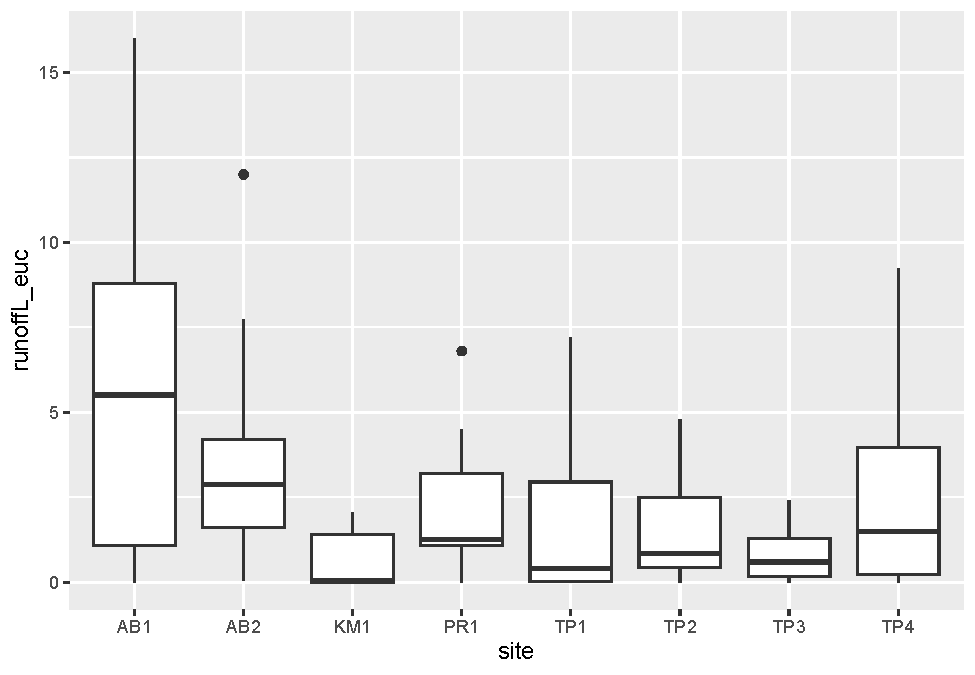
\includegraphics[width=0.75\linewidth]{EnvDataScience_files/figure-latex/absTukeyBoxplot-1} 

}

\caption{Tukey boxplot of runoff under eucalyptus canopy}\label{fig:absTukeyBoxplot}
\end{figure}

\section{Database operations}\label{dplyr}

\index{dplyr}As part of exploring our data, we'll typically simplify or
reduce it for our purposes. The following methods are quickly discovered
to be essential as part of exploring and analyzing data.

\begin{itemize}
\tightlist
\item
  \textbf{select variable columns} you want to retain with \texttt{select}
\item
  \textbf{filter observations} using logic, such as \texttt{population\ \textbackslash{}\textgreater{}\ 10000},
  with \texttt{filter}
\item
  \textbf{subset} data to do both filtering and variable selection, with
  base R's \texttt{subset}
\item
  \textbf{add} new variables and assign their values with \texttt{mutate}
\item
  \textbf{sort} rows based on a field with \texttt{arrange}
\item
  \textbf{summarize} by group
\end{itemize}

\subsection{Select, mutate, and the pipe}\label{pipe}

\index{pipe}\index{\%\>\%}Read the pipe operator \textbf{\texttt{\%\textgreater{}\%}} as ``and
then\ldots{}'' This is bigger than it sounds and opens up many possibilities.

\begin{quote}
You can also use \textbf{\texttt{\textbar{}\textgreater{}}} as the pipe operator. Once you get used to where the \texttt{\textbar{}} character is on your keyboard, you'll find that it makes your code a bit easier to read. \emph{Every character adds up when you're interpreting code.}
\end{quote}

See the example below, and observe how the expression becomes several
lines long. In the process, we'll see examples of new variables with
\index{mutate}mutate and \index{select}selecting (and in the process
\emph{ordering}) variables (Table \ref{tab:eucoak6table}).

\begin{Shaded}
\begin{Highlighting}[]
\NormalTok{runoff }\OtherTok{\textless{}{-}}\NormalTok{ eucoakrainfallrunoffTDR }\SpecialCharTok{\%\textgreater{}\%}
  \FunctionTok{mutate}\NormalTok{(}\AttributeTok{Date =} \FunctionTok{as.Date}\NormalTok{(date,}\StringTok{"\%m/\%d/\%Y"}\NormalTok{),}
         \AttributeTok{rain\_subcanopy =}\NormalTok{ (rain\_oak }\SpecialCharTok{+}\NormalTok{ rain\_euc)}\SpecialCharTok{/}\DecValTok{2}\NormalTok{) }\SpecialCharTok{\%\textgreater{}\%}
\NormalTok{  dplyr}\SpecialCharTok{::}\FunctionTok{select}\NormalTok{(site, Date, rain\_mm, rain\_subcanopy, }
\NormalTok{         runoffL\_oak, runoffL\_euc, slope\_oak, slope\_euc)}
\end{Highlighting}
\end{Shaded}

\begin{table}
\centering
\caption{\label{tab:eucoak6table}EucOak data reorganized a bit, first 6}
\centering
\resizebox{\ifdim\width>\linewidth\linewidth\else\width\fi}{!}{
\begin{tabular}[t]{l|l|r|r|r|r|r|r}
\hline
site & Date & rain\_mm & rain\_subcanopy & runoffL\_oak & runoffL\_euc & slope\_oak & slope\_euc\\
\hline
AB1 & 2006-11-08 & 29 & 29.0 & 4.7900 & 6.70000 & 32 & 31\\
\hline
AB1 & 2006-11-12 & 22 & 18.5 & 3.2000 & 4.30000 & 32 & 31\\
\hline
AB1 & 2006-11-29 & 85 & 65.0 & 9.7000 & 16.00000 & 32 & 31\\
\hline
AB1 & 2006-12-12 & 82 & 87.5 & 14.0000 & 14.20000 & 32 & 31\\
\hline
AB1 & 2006-12-28 & 43 & 54.0 & 9.7472 & 4.32532 & 32 & 31\\
\hline
AB1 & 2007-01-29 & 7 & 54.0 & 1.4000 & 0.00000 & 32 & 31\\
\hline
\end{tabular}}
\end{table}

Another way of thinking of the pipe that is very useful is that whatever
goes before it becomes the first parameter for any functions that
follow. So in the example above:

\begin{enumerate}
\def\labelenumi{\arabic{enumi}.}
\tightlist
\item
  The parameter \texttt{eucoakrainfallrunoffTDR} becomes the first for
  \texttt{mutate()}, then
\item
  The result of the \texttt{mutate()} becomes the first parameter for
  \texttt{dplyr::select()}
\end{enumerate}

\begin{quote}
To just rename a variable, use \texttt{rename} instead of \texttt{mutate}. It will
stay in position.
\end{quote}

\subsubsection{Review: creating penguins from penguins\_raw}\label{review-creating-penguins-from-penguins_raw}

To review some of these methods, it's useful to consider how the
penguins data frame was created from the more complex penguins\_raw data
frame, both of which are part of the
\index{palmerpenguins package}palmerpenguins package (Horst et al. (\citeproc{ref-palmer}{2020})). First
let's look at \texttt{palmerpenguins::penguins\_raw}:

\begin{Shaded}
\begin{Highlighting}[]
\FunctionTok{library}\NormalTok{(palmerpenguins)}
\FunctionTok{library}\NormalTok{(tidyverse)}
\FunctionTok{library}\NormalTok{(lubridate)}
\FunctionTok{summary}\NormalTok{(penguins\_raw)}
\end{Highlighting}
\end{Shaded}

\begin{verbatim}
##      studyName   Sample Number         Species          Region   
##  Length   :344   Min.   :  1.00   Length   :344   Length   :344  
##  N.unique :  3   1st Qu.: 29.00   N.unique :  3   N.unique :  1  
##  N.blank  :  0   Median : 58.00   N.blank  :  0   N.blank  :  0  
##  Min.nchar:  7   Mean   : 63.15   Min.nchar: 33   Min.nchar:  6  
##  Max.nchar:  7   3rd Qu.: 95.25   Max.nchar: 41   Max.nchar:  6  
##                  Max.   :152.00                                  
##                                                                  
##        Island          Stage       Individual ID Clutch Completion
##  Length   :344   Length   :344   Length   :344   Length   :344    
##  N.unique :  3   N.unique :  1   N.unique :190   N.unique :  2    
##  N.blank  :  0   N.blank  :  0   N.blank  :  0   N.blank  :  0    
##  Min.nchar:  5   Min.nchar: 18   Min.nchar:  4   Min.nchar:  2    
##  Max.nchar:  9   Max.nchar: 18   Max.nchar:  6   Max.nchar:  3    
##                                                                   
##                                                                   
##     Date Egg          Culmen Length (mm) Culmen Depth (mm) Flipper Length (mm)
##  Min.   :2007-11-09   Min.   :32.10      Min.   :13.10     Min.   :172.0      
##  1st Qu.:2007-11-28   1st Qu.:39.23      1st Qu.:15.60     1st Qu.:190.0      
##  Median :2008-11-09   Median :44.45      Median :17.30     Median :197.0      
##  Mean   :2008-11-27   Mean   :43.92      Mean   :17.15     Mean   :200.9      
##  3rd Qu.:2009-11-16   3rd Qu.:48.50      3rd Qu.:18.70     3rd Qu.:213.0      
##  Max.   :2009-12-01   Max.   :59.60      Max.   :21.50     Max.   :231.0      
##                       NAs    :2          NAs    :2         NAs    :2          
##  Body Mass (g)         Sex      Delta 15 N (o/oo) Delta 13 C (o/oo)
##  Min.   :2700   Length   :344   Min.   : 7.632    Min.   :-27.02   
##  1st Qu.:3550   N.unique :  2   1st Qu.: 8.300    1st Qu.:-26.32   
##  Median :4050   N.blank  :  0   Median : 8.652    Median :-25.83   
##  Mean   :4202   Min.nchar:  4   Mean   : 8.733    Mean   :-25.69   
##  3rd Qu.:4750   Max.nchar:  6   3rd Qu.: 9.172    3rd Qu.:-25.06   
##  Max.   :6300   NAs      : 11   Max.   :10.025    Max.   :-23.79   
##  NAs    :2                      NAs    :14        NAs    :13       
##       Comments  
##  Length   :344  
##  N.unique : 10  
##  N.blank  :  0  
##  Min.nchar: 18  
##  Max.nchar: 68  
##  NAs      :290  
## 
\end{verbatim}

Now let's create the simpler penguins data frame. We'll use rename for a
couple, but most variables require mutation to manipulate strings (we'll
get to that later), create factors, or convert to integers. And we'll
rename some variables to avoid using backticks (the backward single
quotation mark accessed just to the left of the \texttt{1} key and below the
\texttt{Esc} key, and what you can use in markdown to create a monospaced font
as I just used for \texttt{1} and \texttt{Esc}).

\begin{Shaded}
\begin{Highlighting}[]
\NormalTok{penguins }\OtherTok{\textless{}{-}}\NormalTok{ penguins\_raw }\SpecialCharTok{\%\textgreater{}\%}
  \FunctionTok{rename}\NormalTok{(}\AttributeTok{bill\_length\_mm =} \StringTok{\textasciigrave{}}\AttributeTok{Culmen Length (mm)}\StringTok{\textasciigrave{}}\NormalTok{,}
         \AttributeTok{bill\_depth\_mm =} \StringTok{\textasciigrave{}}\AttributeTok{Culmen Depth (mm)}\StringTok{\textasciigrave{}}\NormalTok{) }\SpecialCharTok{\%\textgreater{}\%}
  \FunctionTok{mutate}\NormalTok{(}\AttributeTok{species =} \FunctionTok{factor}\NormalTok{(}\FunctionTok{word}\NormalTok{(Species)),}
         \AttributeTok{island =} \FunctionTok{factor}\NormalTok{(Island),}
         \AttributeTok{flipper\_length\_mm =} \FunctionTok{as.integer}\NormalTok{(}\StringTok{\textasciigrave{}}\AttributeTok{Flipper Length (mm)}\StringTok{\textasciigrave{}}\NormalTok{),}
         \AttributeTok{body\_mass\_g =} \FunctionTok{as.integer}\NormalTok{(}\StringTok{\textasciigrave{}}\AttributeTok{Body Mass (g)}\StringTok{\textasciigrave{}}\NormalTok{),}
         \AttributeTok{sex =} \FunctionTok{factor}\NormalTok{(}\FunctionTok{str\_to\_lower}\NormalTok{(Sex)),}
         \AttributeTok{year =} \FunctionTok{as.integer}\NormalTok{(}\FunctionTok{year}\NormalTok{(}\FunctionTok{ymd}\NormalTok{(}\StringTok{\textasciigrave{}}\AttributeTok{Date Egg}\StringTok{\textasciigrave{}}\NormalTok{)))) }\SpecialCharTok{\%\textgreater{}\%}
\NormalTok{  dplyr}\SpecialCharTok{::}\FunctionTok{select}\NormalTok{(species, island, bill\_length\_mm, bill\_depth\_mm, }
\NormalTok{                flipper\_length\_mm, body\_mass\_g, sex, year)}
\FunctionTok{summary}\NormalTok{(penguins)}
\end{Highlighting}
\end{Shaded}

\begin{verbatim}
##       species          island    bill_length_mm  bill_depth_mm  
##  Adelie   :152   Biscoe   :168   Min.   :32.10   Min.   :13.10  
##  Chinstrap: 68   Dream    :124   1st Qu.:39.23   1st Qu.:15.60  
##  Gentoo   :124   Torgersen: 52   Median :44.45   Median :17.30  
##                                  Mean   :43.92   Mean   :17.15  
##                                  3rd Qu.:48.50   3rd Qu.:18.70  
##                                  Max.   :59.60   Max.   :21.50  
##                                  NAs    :2       NAs    :2      
##  flipper_length_mm  body_mass_g       sex           year     
##  Min.   :172.0     Min.   :2700   female:165   Min.   :2007  
##  1st Qu.:190.0     1st Qu.:3550   male  :168   1st Qu.:2007  
##  Median :197.0     Median :4050   NAs   : 11   Median :2008  
##  Mean   :200.9     Mean   :4202                Mean   :2008  
##  3rd Qu.:213.0     3rd Qu.:4750                3rd Qu.:2009  
##  Max.   :231.0     Max.   :6300                Max.   :2009  
##  NAs    :2         NAs    :2
\end{verbatim}

Unfortunately, they don't end up as \emph{exactly}
\index{identical}identical, though all of the variables are identical as
vectors:

\begin{Shaded}
\begin{Highlighting}[]
\FunctionTok{identical}\NormalTok{(penguins, palmerpenguins}\SpecialCharTok{::}\NormalTok{penguins)}
\end{Highlighting}
\end{Shaded}

\begin{verbatim}
## [1] FALSE
\end{verbatim}

\subsubsection{\texorpdfstring{Helper functions for \texttt{dplyr::select()}}{Helper functions for dplyr::select()}}\label{helper-functions-for-dplyrselect}

In the \index{select}\texttt{select()} example above, we listed all of the
variables, but there are a variety of helper functions for using logic
to specify which variables to select:

\begin{itemize}
\tightlist
\item
  \texttt{contains("\_")} or any substring of interest in the variable name
\item
  \texttt{starts\_with("runoff")}
\item
  \texttt{ends\_with("euc")}
\item
  \texttt{everything()}
\item
  \texttt{matches()} a regular expression
\item
  \texttt{num\_range("x",1:5)} for the common situation where a series of
  variable names combine a string and a number
\item
  \texttt{one\_of(myList)} for when you have a group of variable names
\item
  \emph{range} of variables: e.g.~\texttt{runoffL\_oak:slope\_euc} could have
  followed \texttt{rain\_subcanopy} above
\item
  \emph{all but}: preface a variable or a set of variable names with
  \textbf{\texttt{-}} to select all others
\end{itemize}

\subsection{Filtering observations}\label{filter}

\index{filter}\texttt{filter} lets you select observations that meet criteria,
similar to an SQL \texttt{WHERE} clause (Table
\ref{tab:absDateFilteredEucOak}).

\begin{Shaded}
\begin{Highlighting}[]
\NormalTok{runoff2007 }\OtherTok{\textless{}{-}}\NormalTok{ runoff }\SpecialCharTok{\%\textgreater{}\%}
  \FunctionTok{filter}\NormalTok{(Date }\SpecialCharTok{\textgreater{}=} \FunctionTok{as.Date}\NormalTok{(}\StringTok{"04/01/2007"}\NormalTok{, }\StringTok{"\%m/\%d/\%Y"}\NormalTok{))}
\end{Highlighting}
\end{Shaded}

\begin{table}
\centering
\caption{\label{tab:absDateFilteredEucOak}Date-filtered EucOak data}
\centering
\resizebox{\ifdim\width>\linewidth\linewidth\else\width\fi}{!}{
\begin{tabular}[t]{l|l|r|r|r|r|r|r}
\hline
site & Date & rain\_mm & rain\_subcanopy & runoffL\_oak & runoffL\_euc & slope\_oak & slope\_euc\\
\hline
AB1 & 2007-04-23 & NA & 33.5 & 6.94488 & 9.19892 & 32.0 & 31\\
\hline
AB1 & 2007-05-05 & NA & 31.0 & 6.33568 & 7.43224 & 32.0 & 31\\
\hline
AB2 & 2007-04-23 & 23 & 35.5 & 4.32000 & 2.88000 & 24.0 & 25\\
\hline
AB2 & 2007-05-05 & 11 & 25.5 & 4.98000 & 3.30000 & 24.0 & 25\\
\hline
KM1 & 2007-04-23 & NA & 37.0 & 1.56000 & 2.04000 & 30.5 & 25\\
\hline
KM1 & 2007-05-05 & 28 & 22.0 & 1.32000 & 1.32000 & 30.5 & 25\\
\hline
\end{tabular}}
\end{table}

\subsubsection{\texorpdfstring{Filtering out \texttt{NA} with \texttt{!is.na}}{Filtering out NA with !is.na}}\label{filtering-out-na-with-is.na}

\index{is.na}Here's a really important one. There are many times you
need to avoid \texttt{NA}s. We thus commonly see summary statistics using
\texttt{na.rm\ =\ TRUE} in order to \emph{ignore} \texttt{NA}s when calculating a statistic
like \texttt{mean}.

To simply filter out NAs from a vector or a variable use a filter:

\begin{Shaded}
\begin{Highlighting}[]
\NormalTok{feb\_filt }\OtherTok{\textless{}{-}}\NormalTok{ sierraFeb }\SpecialCharTok{\%\textgreater{}\%} \FunctionTok{filter}\NormalTok{(}\SpecialCharTok{!}\FunctionTok{is.na}\NormalTok{(TEMPERATURE))}
\end{Highlighting}
\end{Shaded}

\subsection{\texorpdfstring{Subsetting data with base R's \texttt{subset}}{Subsetting data with base R's subset}}\label{subsetting-data-with-base-rs-subset}

We've looked at selecting variables and filtering observations, both
examples of \emph{subsetting} data. We also learned in the previous chapter
on base R methods that there are lots of ways of subsetting data, such
as using accessors like \texttt{{[}{]}} and \texttt{\$}. We'll look at another base R
method that can do both variable selection and observation filtering in
one step, which in some cases you might prefer.

Let's look at a problem where we're subsetting the
\texttt{palmerpenguins::pengins} data to just abstract the species and body
mass of female penguins. We'd need to use both \texttt{filter} and \texttt{select} to
accomplish this, but of course the pipe operator helps:

\begin{Shaded}
\begin{Highlighting}[]
\FunctionTok{library}\NormalTok{(palmerpenguins); }\FunctionTok{library}\NormalTok{(dplyr)}
\NormalTok{penguins }\SpecialCharTok{|\textgreater{}} \FunctionTok{filter}\NormalTok{(sex}\SpecialCharTok{==}\StringTok{"female"}\NormalTok{) }\SpecialCharTok{|\textgreater{}} \FunctionTok{select}\NormalTok{(species,body\_mass\_g)}
\end{Highlighting}
\end{Shaded}

The exact same result can be achieved with base R's \texttt{subset} function,
which if we use a pipe operator looks pretty similar:

\begin{Shaded}
\begin{Highlighting}[]
\FunctionTok{library}\NormalTok{(palmerpenguins)}
\NormalTok{penguins }\SpecialCharTok{|\textgreater{}} \FunctionTok{subset}\NormalTok{(sex}\SpecialCharTok{==}\StringTok{"female"}\NormalTok{, }\AttributeTok{select=}\FunctionTok{c}\NormalTok{(species,body\_mass\_g))}
\end{Highlighting}
\end{Shaded}

\begin{verbatim}
## # A tibble: 165 x 2
##    species body_mass_g
##    <fct>         <int>
##  1 Adelie         3800
##  2 Adelie         3250
##  3 Adelie         3450
##  4 Adelie         3625
##  5 Adelie         3200
##  6 Adelie         3700
##  7 Adelie         3450
##  8 Adelie         3325
##  9 Adelie         3400
## 10 Adelie         3800
## # i 155 more rows
\end{verbatim}

\begin{quote}
As a review, how would you do this without the pipe?
\end{quote}

Given the option of either using \texttt{filter} and \texttt{select} or just \texttt{subset}
in the above example, it's just personal preference, which is often
driven by the desire to make code readable, and that can go either way.
Then there's the desire to reduce the size of what functions you want to
remember, which can also go either way; you still need to know what
``select'' means.

Let's take our example a bit further and use \texttt{subset} to pick the most
massive individual female penguin in the dataset. You could also do this
with \texttt{filter}, but the key is using the \texttt{max} function.

\begin{Shaded}
\begin{Highlighting}[]
\FunctionTok{library}\NormalTok{(palmerpenguins)}
\NormalTok{penguins }\SpecialCharTok{|\textgreater{}} \FunctionTok{subset}\NormalTok{(sex}\SpecialCharTok{==}\StringTok{"female"}\NormalTok{, }\AttributeTok{select=}\FunctionTok{c}\NormalTok{(species,body\_mass\_g)) }\SpecialCharTok{|\textgreater{}}
            \FunctionTok{subset}\NormalTok{(body\_mass\_g}\SpecialCharTok{==}\FunctionTok{max}\NormalTok{(body\_mass\_g))}
\end{Highlighting}
\end{Shaded}

\begin{verbatim}
## # A tibble: 2 x 2
##   species body_mass_g
##   <fct>         <int>
## 1 Gentoo         5200
## 2 Gentoo         5200
\end{verbatim}

In this case, there was a tie between the two most massive individuals.

\begin{quote}
It shouldn't surprise us that there are lots of ways of subsetting
data in R, since doing so helps us satisfy a key requirement of data
science: being able to wrangle big data into something that is able to
be visualized and understood.
\end{quote}

\subsection{Writing a data frame to a csv}\label{writing-a-data-frame-to-a-csv}

\index{write\_csv}Let's say you have created a data frame, maybe with
read\_csv

\texttt{runoff20062007\ \textless{}-\ read\_csv(ex("eucoak/eucoakrainfallrunoffTDR.csv"))}

Then you do some processing to change it, maybe adding variables,
reorganizing, etc., and you want to write out your new \texttt{eucoak}, so you
just need to use \texttt{write\_csv}

\texttt{write\_csv(eucoak,\ "data/tidy\_eucoak.csv")}

\begin{quote}
\textbf{Note} the use of a data folder \texttt{data}: Remember that your default
workspace (\texttt{wd} for \emph{working directory}) is where your project file
resides (check what it is with \texttt{getwd()}), so by default you're saving
things in that wd. To keep things organized the above code is placing
data in a data folder within the wd.
\end{quote}

\subsection{Summarize by group}\label{group-summary}

\index{summarize by group}\index{stratify}\emph{You'll find that you need to
use this all the time with real data.} Let's say you have a bunch of
data where some \emph{categorical} variable is defining a grouping, like our
site field in the \texttt{eucoak} data. This is a form of \emph{stratifying} our
data\index{stratify}. We'd like to just create average slope, rainfall,
and runoff for each site. Note that it involves two steps, first
defining which field defines the group, then the various summary
statistics we'd like to store. In this case, all of the slopes under
\texttt{oak} remain the same for a given site -- it's a \emph{site} characteristic
-- and the same applies to the \texttt{euc} site, so we can just grab the first
value (mean would have also worked of course) (Table
\ref{tab:absEucOaksummary}).

\begin{Shaded}
\begin{Highlighting}[]
\NormalTok{eucoakSiteAvg }\OtherTok{\textless{}{-}}\NormalTok{ runoff }\SpecialCharTok{\%\textgreater{}\%}
  \FunctionTok{group\_by}\NormalTok{(site) }\SpecialCharTok{\%\textgreater{}\%}
  \FunctionTok{summarize}\NormalTok{(}
    \AttributeTok{rain =} \FunctionTok{mean}\NormalTok{(rain\_mm, }\AttributeTok{na.rm =} \ConstantTok{TRUE}\NormalTok{),}
    \AttributeTok{rain\_subcanopy =} \FunctionTok{mean}\NormalTok{(rain\_subcanopy, }\AttributeTok{na.rm =} \ConstantTok{TRUE}\NormalTok{),}
    \AttributeTok{runoffL\_oak =} \FunctionTok{mean}\NormalTok{(runoffL\_oak, }\AttributeTok{na.rm =} \ConstantTok{TRUE}\NormalTok{),}
    \AttributeTok{runoffL\_euc =} \FunctionTok{mean}\NormalTok{(runoffL\_euc, }\AttributeTok{na.rm =} \ConstantTok{TRUE}\NormalTok{),}
    \AttributeTok{slope\_oak =} \FunctionTok{first}\NormalTok{(slope\_oak),}
    \AttributeTok{slope\_euc =} \FunctionTok{first}\NormalTok{(slope\_euc)}
\NormalTok{  )}
\end{Highlighting}
\end{Shaded}

\begin{table}
\centering
\caption{\label{tab:absEucOaksummary}EucOak data summarized by site}
\centering
\resizebox{\ifdim\width>\linewidth\linewidth\else\width\fi}{!}{
\begin{tabular}[t]{l|r|r|r|r|r|r}
\hline
site & rain & rain\_subcanopy & runoffL\_oak & runoffL\_euc & slope\_oak & slope\_euc\\
\hline
AB1 & 48.37500 & 43.08333 & 6.8018364 & 6.026523 & 32.0 & 31\\
\hline
AB2 & 34.08333 & 35.37500 & 4.9113636 & 3.654545 & 24.0 & 25\\
\hline
KM1 & 48.00000 & 36.12500 & 1.9362500 & 0.592500 & 30.5 & 25\\
\hline
PR1 & 56.50000 & 37.56250 & 0.4585714 & 2.310000 & 27.0 & 23\\
\hline
TP1 & 38.36364 & 30.04545 & 0.8772727 & 1.657273 & 9.0 & 9\\
\hline
TP2 & 34.33333 & 32.86364 & 0.0954545 & 1.525454 & 12.0 & 10\\
\hline
\end{tabular}}
\end{table}

\textbf{Summarizing by group with TRI data}

\begin{Shaded}
\begin{Highlighting}[]
\FunctionTok{library}\NormalTok{(igisci)}
\NormalTok{TRI\_BySite }\OtherTok{\textless{}{-}} \FunctionTok{read\_csv}\NormalTok{(}\FunctionTok{ex}\NormalTok{(}\StringTok{"TRI/TRI\_2017\_CA.csv"}\NormalTok{)) }\SpecialCharTok{\%\textgreater{}\%}
  \FunctionTok{mutate}\NormalTok{(}\AttributeTok{all\_air =} \StringTok{\textasciigrave{}}\AttributeTok{5.1\_FUGITIVE\_AIR}\StringTok{\textasciigrave{}} \SpecialCharTok{+} \StringTok{\textasciigrave{}}\AttributeTok{5.2\_STACK\_AIR}\StringTok{\textasciigrave{}}\NormalTok{) }\SpecialCharTok{\%\textgreater{}\%}
  \FunctionTok{filter}\NormalTok{(all\_air }\SpecialCharTok{\textgreater{}} \DecValTok{0}\NormalTok{) }\SpecialCharTok{\%\textgreater{}\%}
  \FunctionTok{group\_by}\NormalTok{(FACILITY\_NAME) }\SpecialCharTok{\%\textgreater{}\%}
  \FunctionTok{summarize}\NormalTok{(}
    \AttributeTok{FACILITY\_NAME =} \FunctionTok{first}\NormalTok{(FACILITY\_NAME),}
    \AttributeTok{air\_releases =} \FunctionTok{sum}\NormalTok{(all\_air, }\AttributeTok{na.rm =} \ConstantTok{TRUE}\NormalTok{),}
    \AttributeTok{mean\_fugitive =} \FunctionTok{mean}\NormalTok{(}\StringTok{\textasciigrave{}}\AttributeTok{5.1\_FUGITIVE\_AIR}\StringTok{\textasciigrave{}}\NormalTok{, }\AttributeTok{na.rm =} \ConstantTok{TRUE}\NormalTok{), }
    \AttributeTok{LATITUDE =} \FunctionTok{first}\NormalTok{(LATITUDE), }\AttributeTok{LONGITUDE =} \FunctionTok{first}\NormalTok{(LONGITUDE))}
\end{Highlighting}
\end{Shaded}

\begin{quote}
\textbf{Integer} variables might be used to define categories or groups.
Down the road, we'll run into situations where numeric variables might
be used to define groups, such as integer days of the year we'll find
useful in studying time series, but could also be zip codes, census
tracts, or other spatial enumeration units. Note that these are
\emph{discrete}, not \emph{continuous} values.
\end{quote}

\subsection{Count}\label{count}

The \index{count}\texttt{count} function is a simple variant on summarizing by
group, since the only statistic is the count of events. The factor to
group by is simply provided as a parameter: \texttt{count(}\emph{factor}\texttt{)}.

\begin{Shaded}
\begin{Highlighting}[]
\NormalTok{tidy\_eucoak }\SpecialCharTok{\%\textgreater{}\%} \FunctionTok{count}\NormalTok{(tree)}
\end{Highlighting}
\end{Shaded}

\begin{verbatim}
## # A tibble: 2 x 2
##   tree      n
##   <chr> <int>
## 1 euc      90
## 2 oak      90
\end{verbatim}

Another way to create a count is to use \texttt{n()}:

\begin{Shaded}
\begin{Highlighting}[]
\NormalTok{tidy\_eucoak }\SpecialCharTok{\%\textgreater{}\%}
  \FunctionTok{group\_by}\NormalTok{(tree) }\SpecialCharTok{\%\textgreater{}\%}
  \FunctionTok{summarize}\NormalTok{(}\AttributeTok{n =} \FunctionTok{n}\NormalTok{())}
\end{Highlighting}
\end{Shaded}

\begin{verbatim}
## # A tibble: 2 x 2
##   tree      n
##   <chr> <int>
## 1 euc      90
## 2 oak      90
\end{verbatim}

\subsection{Sorting after summarizing}\label{sorting-after-summarizing}

\index{arrange}\index{sort}Using the marine debris data from the \emph{Marine
Debris Monitoring and Assessment Project} (\citeproc{ref-marineDebris}{\emph{Marine Debris Program}, n.d.}), we can use
\texttt{arrange} to sort by latitude, so we can see the beaches from south to
north along the Pacific coast.

\begin{Shaded}
\begin{Highlighting}[]
\NormalTok{shorelineLatLong }\OtherTok{\textless{}{-}}\NormalTok{ ConcentrationReport }\SpecialCharTok{\%\textgreater{}\%}
  \FunctionTok{group\_by}\NormalTok{(}\StringTok{\textasciigrave{}}\AttributeTok{Shoreline Name}\StringTok{\textasciigrave{}}\NormalTok{) }\SpecialCharTok{\%\textgreater{}\%}
  \FunctionTok{summarize}\NormalTok{(}
    \AttributeTok{latitude =} \FunctionTok{mean}\NormalTok{((}\StringTok{\textasciigrave{}}\AttributeTok{Latitude Start}\StringTok{\textasciigrave{}}\SpecialCharTok{+}\StringTok{\textasciigrave{}}\AttributeTok{Latitude End}\StringTok{\textasciigrave{}}\NormalTok{)}\SpecialCharTok{/}\DecValTok{2}\NormalTok{),}
    \AttributeTok{longitude =} \FunctionTok{mean}\NormalTok{((}\StringTok{\textasciigrave{}}\AttributeTok{Longitude Start}\StringTok{\textasciigrave{}}\SpecialCharTok{+}\StringTok{\textasciigrave{}}\AttributeTok{Longitude End}\StringTok{\textasciigrave{}}\NormalTok{)}\SpecialCharTok{/}\DecValTok{2}\NormalTok{)}
\NormalTok{  ) }\SpecialCharTok{\%\textgreater{}\%}
  \FunctionTok{arrange}\NormalTok{(latitude)}
\NormalTok{shorelineLatLong}
\end{Highlighting}
\end{Shaded}

\begin{verbatim}
## # A tibble: 38 x 3
##    `Shoreline Name`   latitude longitude
##    <chr>                 <dbl>     <dbl>
##  1 Aimee Arvidson         33.6     -118.
##  2 Balboa Pier #2         33.6     -118.
##  3 Bolsa Chica            33.7     -118.
##  4 Junipero Beach         33.8     -118.
##  5 Malaga Cove            33.8     -118.
##  6 Zuma Beach, Malibu     34.0     -119.
##  7 Zuma Beach             34.0     -119.
##  8 Will Rodgers           34.0     -119.
##  9 Carbon Beach           34.0     -119.
## 10 Nicholas Canyon        34.0     -119.
## # i 28 more rows
\end{verbatim}

\subsection{The dot operator}\label{the-dot-operator}

\index{dot operator}\index{dot operator}The dot (\textbf{\texttt{.}}) operator
refers to \emph{here}, similar to UNIX syntax for accessing files in the
current folder where the path is \texttt{"./filename"}. In a piped sequence,
you might need to reference the object (like the data frame) the pipe is
using, as you can see in the following code.

\begin{itemize}
\tightlist
\item
  The advantage of the pipe is you don't have to keep referencing the
  data frame.
\item
  The dot is then used to connect to items inside the data frame
\end{itemize}

\begin{Shaded}
\begin{Highlighting}[]
\NormalTok{TRI87 }\OtherTok{\textless{}{-}} \FunctionTok{read\_csv}\NormalTok{(}\FunctionTok{ex}\NormalTok{(}\StringTok{"TRI/TRI\_1987\_BaySites.csv"}\NormalTok{))}
\NormalTok{stackrate }\OtherTok{\textless{}{-}}\NormalTok{ TRI87 }\SpecialCharTok{\%\textgreater{}\%}
  \FunctionTok{mutate}\NormalTok{(}\AttributeTok{stackrate =}\NormalTok{ stack\_air}\SpecialCharTok{/}\NormalTok{air\_releases) }\SpecialCharTok{\%\textgreater{}\%}
\NormalTok{  .}\SpecialCharTok{$}\NormalTok{stackrate}
\FunctionTok{head}\NormalTok{(stackrate)}
\end{Highlighting}
\end{Shaded}

\begin{verbatim}
## [1] 0.0000000 0.0000000 0.0000000 0.0000000 0.6666667 1.0000000
\end{verbatim}

\section{String abstraction}\label{stringr}

\index{string abstraction}Character string manipulation is surprisingly
critical to data analysis, and so the \index{stringr}\textbf{\texttt{stringr}}
package was developed to provide a wider array of string processing
tools than what is in base R, including functions for detecting matches,
subsetting strings, managing lengths, replacing substrings with other
text, and joining, splitting, and sorting strings.

We'll look at some of the \texttt{stringr} functions, but a good way to learn
about the wide array of functions is through the cheat sheet that can be
downloaded from \url{https://www.rstudio.com/resources/cheatsheets/}

\subsection{Detecting matches}\label{detecting-matches}

\index{string matches}These functions look for patterns within existing
strings, which can then be used subset observations based on those
patterns.

\begin{itemize}
\tightlist
\item
  \textbf{\texttt{str\_detect}} detects patterns in a string, returns true or false
  if detected
\item
  \textbf{\texttt{str\_locate}} detects patterns in a string, returns \textbf{start}
  \emph{and} \textbf{end} position if detected, or NA if not
\item
  \textbf{\texttt{str\_which}} returns the indices of strings that match a pattern
\item
  \textbf{\texttt{str\_count}} counts the number of matches in each string
\end{itemize}

\begin{Shaded}
\begin{Highlighting}[]
\FunctionTok{str\_detect}\NormalTok{(fruit,}\StringTok{"qu"}\NormalTok{)}
\FunctionTok{str\_which}\NormalTok{(fruit, }\StringTok{"qu"}\NormalTok{)}
\NormalTok{fruit[}\FunctionTok{str\_which}\NormalTok{(fruit,}\StringTok{"qu"}\NormalTok{)]}
\end{Highlighting}
\end{Shaded}

\begin{verbatim}
##  [1] FALSE FALSE FALSE FALSE FALSE FALSE FALSE FALSE FALSE FALSE FALSE FALSE
## [13] FALSE FALSE FALSE FALSE FALSE FALSE FALSE FALSE FALSE FALSE FALSE FALSE
## [25] FALSE FALSE FALSE FALSE FALSE FALSE FALSE FALSE FALSE FALSE FALSE FALSE
## [37] FALSE FALSE FALSE FALSE FALSE FALSE  TRUE FALSE FALSE  TRUE FALSE FALSE
## [49] FALSE FALSE FALSE FALSE FALSE FALSE FALSE FALSE FALSE FALSE FALSE FALSE
## [61] FALSE FALSE FALSE FALSE FALSE FALSE  TRUE FALSE FALSE FALSE FALSE FALSE
## [73] FALSE FALSE FALSE FALSE FALSE FALSE FALSE FALSE
## [1] 43 46 67
## [1] "kumquat" "loquat"  "quince"
\end{verbatim}

Note that \texttt{str\_locate} returns a matrix with rows for each item where
the substring is located with both \texttt{start} and \texttt{end} locations.

\begin{Shaded}
\begin{Highlighting}[]
\NormalTok{fruit\_a }\OtherTok{\textless{}{-}}\NormalTok{ fruit[}\FunctionTok{str\_count}\NormalTok{(fruit,}\StringTok{"a"}\NormalTok{)}\SpecialCharTok{\textgreater{}}\DecValTok{1}\NormalTok{]}
\NormalTok{fruit\_a}
\FunctionTok{str\_locate}\NormalTok{(fruit\_a,}\StringTok{"a"}\NormalTok{)}
\end{Highlighting}
\end{Shaded}

\begin{verbatim}
##  [1] "avocado"      "banana"       "blackcurrant" "canary melon" "cantaloupe"  
##  [6] "guava"        "mandarine"    "papaya"       "pomegranate"  "rambutan"    
## [11] "salal berry"  "satsuma"      "tamarillo"   
##       start end
##  [1,]     1   1
##  [2,]     2   2
##  [3,]     3   3
##  [4,]     2   2
##  [5,]     2   2
##  [6,]     3   3
##  [7,]     2   2
##  [8,]     2   2
##  [9,]     7   7
## [10,]     2   2
## [11,]     2   2
## [12,]     2   2
## [13,]     2   2
\end{verbatim}

The \texttt{str\_locate\_all} function carries this further and finds all
locations of the substrings within the string.

\begin{Shaded}
\begin{Highlighting}[]
\NormalTok{fruit3a }\OtherTok{\textless{}{-}}\NormalTok{ fruit[}\FunctionTok{str\_count}\NormalTok{(fruit,}\StringTok{"a"}\NormalTok{)}\SpecialCharTok{==}\DecValTok{3}\NormalTok{]}
\NormalTok{fruit3a}
\FunctionTok{str\_locate\_all}\NormalTok{(fruit3a,}\StringTok{"a"}\NormalTok{)}
\end{Highlighting}
\end{Shaded}

\begin{verbatim}
## [1] "banana" "papaya"
## [[1]]
##      start end
## [1,]     2   2
## [2,]     4   4
## [3,]     6   6
## 
## [[2]]
##      start end
## [1,]     2   2
## [2,]     4   4
## [3,]     6   6
\end{verbatim}

\begin{Shaded}
\begin{Highlighting}[]
\NormalTok{qufruit }\OtherTok{\textless{}{-}}\NormalTok{ fruit[}\FunctionTok{str\_which}\NormalTok{(fruit,}\StringTok{"qu"}\NormalTok{)]}
\NormalTok{qufruit}
\FunctionTok{str\_locate}\NormalTok{(qufruit, }\StringTok{"qu"}\NormalTok{)}
\end{Highlighting}
\end{Shaded}

\begin{verbatim}
## [1] "kumquat" "loquat"  "quince" 
##      start end
## [1,]     4   5
## [2,]     3   4
## [3,]     1   2
\end{verbatim}

\subsection{Subsetting strings}\label{subset-string}

\index{string subsetting}Subsetting in this case includes its normal use
of abstracting the observations specified by a match (similar to a
filter for data frames), or just a specified part of a string specified
by start and end character positions, or the part of the string that
matches an expression.

\begin{itemize}
\tightlist
\item
  \textbf{\texttt{str\_sub}} extracts a part of a string from a start to an end
  character position
\item
  \textbf{\texttt{str\_subset}} returns the strings that contain a pattern match
\item
  \textbf{\texttt{str\_extract}} returns the first (or if \texttt{str\_extract\_all} then
  all matches) pattern matches
\item
  \textbf{\texttt{str\_match}} returns the first (or \texttt{\_all}) pattern match as a
  matrix
\item
  \textbf{\texttt{str\_remove}} removes a specific substring (not on the cheat
  sheet, but handy)
\end{itemize}

\begin{Shaded}
\begin{Highlighting}[]
\NormalTok{qfruit }\OtherTok{\textless{}{-}} \FunctionTok{str\_subset}\NormalTok{(fruit, }\StringTok{"q"}\NormalTok{)}
\NormalTok{qfruit}
\FunctionTok{str\_sub}\NormalTok{(qfruit,}\DecValTok{1}\NormalTok{,}\DecValTok{2}\NormalTok{)}
\end{Highlighting}
\end{Shaded}

\begin{verbatim}
## [1] "kumquat" "loquat"  "quince" 
## [1] "ku" "lo" "qu"
\end{verbatim}

\begin{Shaded}
\begin{Highlighting}[]
\FunctionTok{str\_sub}\NormalTok{(}\StringTok{"94132"}\NormalTok{,}\DecValTok{1}\NormalTok{,}\DecValTok{2}\NormalTok{)}
\FunctionTok{str\_extract}\NormalTok{(qfruit,}\StringTok{"[aeiou]"}\NormalTok{)}
\FunctionTok{str\_remove}\NormalTok{(}\FunctionTok{str\_subset}\NormalTok{(fruit,}\StringTok{"fruit"}\NormalTok{), }\StringTok{"fruit"}\NormalTok{)}
\end{Highlighting}
\end{Shaded}

\begin{verbatim}
## [1] "94"
## [1] "u" "o" "u"
## [1] "bread"   "dragon"  "grape"   "jack"    "kiwi "   "passion" "star "  
## [8] "ugli "
\end{verbatim}

\subsection{String length}\label{string-length}

\index{string length}The length of strings is often useful in an
analysis process, either just knowing the length as an integer, or
purposefully increasing or reducing it.

\begin{itemize}
\tightlist
\item
  \textbf{\texttt{str\_length}} \index{str\_length}simply returns the length of the
  string as an integer
\end{itemize}

\begin{Shaded}
\begin{Highlighting}[]
\NormalTok{qfruit }\OtherTok{\textless{}{-}} \FunctionTok{str\_subset}\NormalTok{(fruit,}\StringTok{"q"}\NormalTok{)}
\NormalTok{qfruit}
\FunctionTok{str\_length}\NormalTok{(qfruit)}
\end{Highlighting}
\end{Shaded}

\begin{verbatim}
## [1] "kumquat" "loquat"  "quince" 
## [1] 7 6 6
\end{verbatim}

Don't confuse \texttt{str\_length} with \texttt{length} (from base R), the length of an object like a vector. Both are highly useful.

\begin{Shaded}
\begin{Highlighting}[]
\FunctionTok{length}\NormalTok{(fruit)}
\end{Highlighting}
\end{Shaded}

\begin{verbatim}
## [1] 80
\end{verbatim}

\begin{Shaded}
\begin{Highlighting}[]
\FunctionTok{length}\NormalTok{(qfruit)}
\end{Highlighting}
\end{Shaded}

\begin{verbatim}
## [1] 3
\end{verbatim}

Using \texttt{str\_locate} with \texttt{str\_length}:

\begin{Shaded}
\begin{Highlighting}[]
\NormalTok{name }\OtherTok{\textless{}{-}} \StringTok{"Inigo Montoya"}
\FunctionTok{str\_length}\NormalTok{(name)}
\NormalTok{firstname }\OtherTok{\textless{}{-}} \FunctionTok{str\_sub}\NormalTok{(name,}\DecValTok{1}\NormalTok{,}\FunctionTok{str\_locate}\NormalTok{(name,}\StringTok{" "}\NormalTok{)[}\DecValTok{1}\NormalTok{]}\SpecialCharTok{{-}}\DecValTok{1}\NormalTok{)}
\NormalTok{firstname}
\NormalTok{lastname }\OtherTok{\textless{}{-}} \FunctionTok{str\_sub}\NormalTok{(name,}\FunctionTok{str\_locate}\NormalTok{(name,}\StringTok{" "}\NormalTok{)[}\DecValTok{1}\NormalTok{]}\SpecialCharTok{+}\DecValTok{1}\NormalTok{,}\FunctionTok{str\_length}\NormalTok{(name))}
\NormalTok{lastname}
\end{Highlighting}
\end{Shaded}

\begin{verbatim}
## [1] 13
## [1] "Inigo"
## [1] "Montoya"
\end{verbatim}

\textbf{Padding and trimming lengths}:

\begin{itemize}
\tightlist
\item
  \textbf{\texttt{str\_pad}} \index{string pad}adds a specified character
  (typically a space \texttt{"\ "}) to either end of a string
\item
  \textbf{\texttt{str\_trim}} \index{string trim}removes white space from either
  end of a string
\end{itemize}

Here's an example \texttt{str\_pad} and \texttt{str\_trim} (in this case, reversing the
former):

\begin{Shaded}
\begin{Highlighting}[]
\FunctionTok{str\_pad}\NormalTok{(qfruit,}\DecValTok{10}\NormalTok{,}\StringTok{"both"}\NormalTok{)}
\FunctionTok{str\_trim}\NormalTok{(}\FunctionTok{str\_pad}\NormalTok{(qfruit,}\DecValTok{10}\NormalTok{,}\StringTok{"both"}\NormalTok{),}\StringTok{"both"}\NormalTok{)}
\end{Highlighting}
\end{Shaded}

\begin{verbatim}
## [1] " kumquat  " "  loquat  " "  quince  "
## [1] "kumquat" "loquat"  "quince"
\end{verbatim}

\subsection{Replacing substrings with other text (``mutating'' strings)}\label{replacing-substrings-with-other-text-mutating-strings}

\index{string substring replacement}These methods range from converting
case to replacing substrings.

\begin{itemize}
\tightlist
\item
  \textbf{\texttt{str\_to\_lower}} converts strings to lowercase
\item
  \textbf{\texttt{str\_to\_upper}} converts strings to uppercase
\item
  \textbf{\texttt{str\_to\_title}} capitalizes strings (makes the first character of
  each word uppercase)
\end{itemize}

\begin{Shaded}
\begin{Highlighting}[]
\FunctionTok{str\_to\_lower}\NormalTok{(name)}
\FunctionTok{str\_to\_upper}\NormalTok{(name)}
\FunctionTok{str\_to\_title}\NormalTok{(}\StringTok{"for whom the bell tolls"}\NormalTok{)}
\end{Highlighting}
\end{Shaded}

\begin{verbatim}
## [1] "inigo montoya"
## [1] "INIGO MONTOYA"
## [1] "For Whom The Bell Tolls"
\end{verbatim}

\begin{itemize}
\tightlist
\item
  \textbf{\texttt{str\_replace}} replaces the first matched pattern (or all with
  \texttt{str\_replace\_all}) with a specified string
\item
  \textbf{\texttt{str\_sub}} a special use of this function to replace substrings
  with a specified string
\end{itemize}

\begin{Shaded}
\begin{Highlighting}[]
\FunctionTok{str\_replace}\NormalTok{(qfruit,}\StringTok{"q"}\NormalTok{,}\StringTok{"z"}\NormalTok{)}
\FunctionTok{str\_sub}\NormalTok{(name,}\DecValTok{1}\NormalTok{,}\FunctionTok{str\_locate}\NormalTok{(name,}\StringTok{" "}\NormalTok{)[}\DecValTok{1}\NormalTok{]}\SpecialCharTok{{-}}\DecValTok{1}\NormalTok{) }\OtherTok{\textless{}{-}} \StringTok{"Diego"}
\NormalTok{name}
\end{Highlighting}
\end{Shaded}

\begin{verbatim}
## [1] "kumzuat" "lozuat"  "zuince" 
## [1] "Diego Montoya"
\end{verbatim}

\begin{quote}
The replacement mode of \texttt{str\_sub} used above may seem pretty tortuous
and confusing. Why did we have to access \texttt{{[}1{]}} in
\texttt{str\_locate(name,"\ "){[}1{]}}? Experiment with what you get with
\texttt{str\_locate(name,"\ ")} itself, and maybe consult the help system with
\texttt{?str\_locate} (and run the examples), but you'll find this is one that
returns a matrix, and even if there's only one item located will still
have a \texttt{start} and \texttt{end} location. See what happens when you use it
\emph{without} accessing \texttt{{[}1{]}}. You're seeing one effect of vectorization
-- \textbf{reuse}. It can be very confusing, but reuse of inputs is one of
the (very useful but still confusing) properties of vectorization. In
this case it creates duplication, creating a vector of names.
\end{quote}

\subsection{Concatenating and splitting}\label{concatenating-and-splitting}

\index{string concatenating and splitting}One very common string
function is to concatenate strings, and somewhat less common is
splitting them using a key separator like space, comma, or line end. One
use of using str\_c in the example below is to create a comparable join
field based on a numeric character string that might need a zero or
something at the left or right.

\begin{itemize}
\tightlist
\item
  \textbf{\texttt{str\_c}} \index{str\_c}The \texttt{paste()} function in base R will
  work, but you might want the default separator setting to be ``\,'' (as
  does \texttt{paste0()}) instead of \texttt{"\ "}, so \texttt{str\_c} is just \texttt{paste} with a
  default ``\,'' separator, but you can also use \texttt{"\ "}.
\item
  \textbf{\texttt{str\_split}} \index{str\_split}splits a string into parts based
  upon the detection of a specified separator like space, comma, or
  line end. However, this ends up creating a list, which can be
  confusing to use. If you're wanting to access a particular member of
  a list of words, the \texttt{word} function is easier.
\item
  \textbf{\texttt{word}} \index{word}lets you pick the first, second, or nth word
  in a string of words.
\end{itemize}

\begin{Shaded}
\begin{Highlighting}[]
\FunctionTok{library}\NormalTok{(stringr)}
\NormalTok{phrase }\OtherTok{\textless{}{-}} \FunctionTok{str\_c}\NormalTok{(}\StringTok{"for"}\NormalTok{,}\StringTok{"whom"}\NormalTok{,}\StringTok{"the"}\NormalTok{,}\StringTok{"bell"}\NormalTok{,}\StringTok{"tolls"}\NormalTok{,}\AttributeTok{sep=}\StringTok{" "}\NormalTok{)}
\NormalTok{phrase}
\end{Highlighting}
\end{Shaded}

\begin{verbatim}
## [1] "for whom the bell tolls"
\end{verbatim}

\begin{Shaded}
\begin{Highlighting}[]
\FunctionTok{str\_split}\NormalTok{(phrase, }\StringTok{" "}\NormalTok{)}
\end{Highlighting}
\end{Shaded}

\begin{verbatim}
## [[1]]
## [1] "for"   "whom"  "the"   "bell"  "tolls"
\end{verbatim}

\begin{Shaded}
\begin{Highlighting}[]
\FunctionTok{word}\NormalTok{(phrase,}\DecValTok{4}\NormalTok{)}
\end{Highlighting}
\end{Shaded}

\begin{verbatim}
## [1] "bell"
\end{verbatim}

\ldots{} and of course, these methods can all be
\index{vectorized}vectorized:

\begin{Shaded}
\begin{Highlighting}[]
\NormalTok{sentences[}\DecValTok{1}\SpecialCharTok{:}\DecValTok{4}\NormalTok{]}
\end{Highlighting}
\end{Shaded}

\begin{verbatim}
## [1] "The birch canoe slid on the smooth planks." 
## [2] "Glue the sheet to the dark blue background."
## [3] "It's easy to tell the depth of a well."     
## [4] "These days a chicken leg is a rare dish."
\end{verbatim}

\begin{Shaded}
\begin{Highlighting}[]
\FunctionTok{word}\NormalTok{(sentences[}\DecValTok{1}\SpecialCharTok{:}\DecValTok{4}\NormalTok{],}\DecValTok{2}\NormalTok{)}
\end{Highlighting}
\end{Shaded}

\begin{verbatim}
## [1] "birch" "the"   "easy"  "days"
\end{verbatim}

Example of \texttt{str\_c} use to modify a variable needed for a join:

\begin{Shaded}
\begin{Highlighting}[]
\NormalTok{csvPath }\OtherTok{\textless{}{-}} \FunctionTok{system.file}\NormalTok{(}\StringTok{"extdata"}\NormalTok{,}\StringTok{"CA/CA\_MdInc.csv"}\NormalTok{,}\AttributeTok{package=}\StringTok{"igisci"}\NormalTok{)}
\NormalTok{CA\_MdInc }\OtherTok{\textless{}{-}} \FunctionTok{read\_csv}\NormalTok{(csvPath)}
\NormalTok{join\_id }\OtherTok{\textless{}{-}} \FunctionTok{str\_c}\NormalTok{(}\StringTok{"0"}\NormalTok{,CA\_MdInc}\SpecialCharTok{$}\NormalTok{NAME)}
\CommentTok{\# could also use str\_pad(CA\_MdInc$NAME,1,side="left",pad="0")}
\FunctionTok{head}\NormalTok{(CA\_MdInc)}
\end{Highlighting}
\end{Shaded}

\begin{verbatim}
## # A tibble: 6 x 3
##         trID     NAME HHinc2016
##        <dbl>    <dbl>     <dbl>
## 1 6001400100 60014001    177417
## 2 6001400200 60014002    153125
## 3 6001400300 60014003     85313
## 4 6001400400 60014004     99539
## 5 6001400500 60014005     83650
## 6 6001400600 60014006     61597
\end{verbatim}

\begin{Shaded}
\begin{Highlighting}[]
\FunctionTok{head}\NormalTok{(join\_id)}
\end{Highlighting}
\end{Shaded}

\begin{verbatim}
## [1] "060014001" "060014002" "060014003" "060014004" "060014005" "060014006"
\end{verbatim}

\section{\texorpdfstring{Dates and times with \texttt{lubridate}}{Dates and times with lubridate}}\label{lubridate}

\index{dates and times}Simply stated, the \index{lubridate}\texttt{lubridate}
package just makes it easier to work with dates and times. Dates and
times are more difficult to work with than numbers and character
strings, which is why \texttt{lubridate} was developed. The \texttt{lubridate} package
is excellent at detecting and reading in dates and times -- it can
``parse'' many forms. Spend some time to make sure you know how to use it.
We'll be using dates and times a lot, since many data sets include time
stamps. See the cheat sheet for more information but the following
examples may demonstrate that it's pretty easy to use, and does a good
job of making your job easier.

\begin{Shaded}
\begin{Highlighting}[]
\FunctionTok{library}\NormalTok{(lubridate)}
\FunctionTok{dmy}\NormalTok{(}\StringTok{"20 September 2020"}\NormalTok{)}
\FunctionTok{dmy\_hm}\NormalTok{(}\StringTok{"20 September 2020 10:45"}\NormalTok{)}
\FunctionTok{mdy\_hms}\NormalTok{(}\StringTok{"September 20, 2020 10:48"}\NormalTok{)}
\FunctionTok{mdy\_hm}\NormalTok{(}\StringTok{"9/20/20 10:50"}\NormalTok{)}
\FunctionTok{mdy}\NormalTok{(}\StringTok{"9.20.20"}\NormalTok{)}
\end{Highlighting}
\end{Shaded}

\begin{verbatim}
## [1] "2020-09-20"
## [1] "2020-09-20 10:45:00 UTC"
## [1] "2020-09-20 20:10:48 UTC"
## [1] "2020-09-20 10:50:00 UTC"
## [1] "2020-09-20"
\end{verbatim}

\begin{Shaded}
\begin{Highlighting}[]
\NormalTok{start704 }\OtherTok{\textless{}{-}} \FunctionTok{dmy\_hm}\NormalTok{(}\StringTok{"24 August 2020 16:00"}\NormalTok{)}
\NormalTok{end704 }\OtherTok{\textless{}{-}} \FunctionTok{mdy\_hm}\NormalTok{(}\StringTok{"12/18/2020 4:45 pm"}\NormalTok{)}
\FunctionTok{year}\NormalTok{(start704)}
\FunctionTok{month}\NormalTok{(start704)}
\FunctionTok{day}\NormalTok{(end704)}
\FunctionTok{hour}\NormalTok{(end704)}
\end{Highlighting}
\end{Shaded}

\begin{verbatim}
## [1] 2020
## [1] 8
## [1] 18
## [1] 16
\end{verbatim}

A bit of date math:

\begin{Shaded}
\begin{Highlighting}[]
\NormalTok{end704}\SpecialCharTok{{-}}\NormalTok{start704}
\FunctionTok{as\_date}\NormalTok{(end704)}
\NormalTok{hms}\SpecialCharTok{::}\FunctionTok{as\_hms}\NormalTok{(end704)}
\end{Highlighting}
\end{Shaded}

\begin{verbatim}
## Time difference of 116.0312 days
## [1] "2020-12-18"
## 16:45:00
\end{verbatim}

You will find that dates are typically displayed as yyyy-mm-dd, e.g.
``2020-09-20'' above. You can display them other ways of course, but it's
useful to write dates this way since they sort better, with the highest
order coming first.

\index{explicit function calls}

\begin{quote}
Calling functions explicitly with \texttt{::}: Sometimes you need to specify
the package and function name this way, for instance, if more than one
package has a function of the same name. You can also use this method
to call a function without having loaded its library. Due to multiple
packages having certain common names (like \texttt{select}), it's common to
use this syntax, and you'll find that we'll use \texttt{dplyr::select(...)}
throughout this book.
\end{quote}

\subsection{Dates used for annual time series}\label{dates-used-for-annual-time-series}

For obvious reasons, we'll use \texttt{lubridate} a lot when we get to time
series. One date abstraction that will be particularly useful is day of
the year, which can be abstracted from a date object as \texttt{yday}, which
returns the day of the year starting with 1 for January 1 in any given
year. Note that as with all of the date objects, you need to work with
actual date objects, which we do in the following example, which creates
a simple data frame table of month, day and day of year, then displays a
subset that illustrates the utility:

\begin{Shaded}
\begin{Highlighting}[]
\FunctionTok{library}\NormalTok{(lubridate)}
\FunctionTok{library}\NormalTok{(tidyverse)}
\NormalTok{Jan1 }\OtherTok{\textless{}{-}} \FunctionTok{ymd}\NormalTok{(}\StringTok{"2022{-}01{-}01"}\NormalTok{)}
\NormalTok{Dec31 }\OtherTok{\textless{}{-}} \FunctionTok{ymd}\NormalTok{(}\StringTok{"2022{-}12{-}31"}\NormalTok{)}
\NormalTok{year2022 }\OtherTok{\textless{}{-}} \FunctionTok{as\_date}\NormalTok{(Jan1}\SpecialCharTok{:}\NormalTok{Dec31)}
\NormalTok{ydayTable }\OtherTok{\textless{}{-}} \FunctionTok{bind\_cols}\NormalTok{(}\AttributeTok{month=}\FunctionTok{month}\NormalTok{(year2022),}\AttributeTok{day=}\FunctionTok{day}\NormalTok{(year2022),}\AttributeTok{doy=}\FunctionTok{yday}\NormalTok{(year2022))}
\NormalTok{ydayTable[}\DecValTok{27}\SpecialCharTok{:}\DecValTok{35}\NormalTok{,] }
\end{Highlighting}
\end{Shaded}

\begin{verbatim}
## # A tibble: 9 x 3
##   month   day   doy
##   <dbl> <int> <dbl>
## 1     1    27    27
## 2     1    28    28
## 3     1    29    29
## 4     1    30    30
## 5     1    31    31
## 6     2     1    32
## 7     2     2    33
## 8     2     3    34
## 9     2     4    35
\end{verbatim}

\section{Extending abstractions with functions}\label{extending-abstractions-with-functions}

We've explored ways of extending base R to facilitate data abstraction,
mostly focusing on the tidyverse in this chapter. There are many other
packages that provide special capabilities, but we can also write our
own, as we explored in the last chapter. Even simple functions of a few
lines of code can make our main code more readable.

We'll look at a simple extension of the \texttt{readxl::read\_excel} function. A
common practice in data logger spreadsheets is to have the variable
names in the first row and the units (like °C or mm in the second row.)
There's no good way to make use of those units in a data frame, so we
typically will want to skip it. The \texttt{read\_excel} function has a \texttt{skip}
parameter that lets us skip the first row, and also the \texttt{col\_names}
parameter that allows us to either use the first row as variable names
(the default, \texttt{TRUE}), get default names (\texttt{FALSE}), or provide a vector
of variable names.

We'll write a function that creates variable names out of the first two
rows, so includes the units with the original variable name by
vectorizing a \texttt{paste0}.

\begin{Shaded}
\begin{Highlighting}[]
\FunctionTok{library}\NormalTok{(igisci); }\FunctionTok{library}\NormalTok{(tidyverse); }\FunctionTok{library}\NormalTok{(readxl)}
\end{Highlighting}
\end{Shaded}

\begin{Shaded}
\begin{Highlighting}[]
\NormalTok{read\_excel2 }\OtherTok{\textless{}{-}} \ControlFlowTok{function}\NormalTok{(xl)\{}
\NormalTok{  vnames }\OtherTok{\textless{}{-}} \FunctionTok{read\_excel}\NormalTok{(xl, }\AttributeTok{n\_max=}\DecValTok{0}\NormalTok{) }\SpecialCharTok{|\textgreater{}} \FunctionTok{names}\NormalTok{()}
\NormalTok{  vunits }\OtherTok{\textless{}{-}} \FunctionTok{read\_excel}\NormalTok{(xl, }\AttributeTok{n\_max=}\DecValTok{0}\NormalTok{, }\AttributeTok{skip=}\DecValTok{1}\NormalTok{) }\SpecialCharTok{|\textgreater{}} \FunctionTok{names}\NormalTok{()}
  \FunctionTok{read\_excel}\NormalTok{(xl, }\AttributeTok{skip=}\DecValTok{2}\NormalTok{, }\AttributeTok{col\_names=}\FunctionTok{paste0}\NormalTok{(vnames,}\StringTok{"\_"}\NormalTok{,vunits))}
\NormalTok{\}}
\end{Highlighting}
\end{Shaded}

Then this is a new function we can just use in our code later on. We'll
be reading this kind of data a lot, so even a short function can make
our main code easier to read.

\begin{Shaded}
\begin{Highlighting}[]
\FunctionTok{read\_excel2}\NormalTok{(}\FunctionTok{ex}\NormalTok{(}\StringTok{"meadows/LoneyMeadow\_30minCO2fluxes\_Geog604.xls"}\NormalTok{))}
\end{Highlighting}
\end{Shaded}

\begin{verbatim}
## # A tibble: 5,397 x 14
##    `Decimal time_mgC m-2 s-1` `Day of Year_mmols m-2 s-1` `Hour of Day_W m-2`
##                         <dbl>                       <dbl>               <dbl>
##  1                       138                          138                24  
##  2                       138.                         138                 0.5
##  3                       138.                         138                 1  
##  4                       138.                         138                 1.5
##  5                       138.                         138                 2  
##  6                       138.                         138                 2.5
##  7                       138.                         138                 3  
##  8                       138.                         138                 3.5
##  9                       138.                         138                 4  
## 10                       138.                         138                 4.5
## # i 5,387 more rows
## # i 11 more variables: `CO2 Flux_degC` <dbl>, `PAR_%` <dbl>, Qnet_degC <dbl>,
## #   Tair_degC <dbl>, RH_deg <dbl>, `Tsoil 2cm_m s-1` <dbl>,
## #   `Tsoil 10cm_mm` <dbl>, `wdir_m3 m-3` <dbl>, `wspd_mgC m-2 s-1` <dbl>,
## #   `Rain_mmols m-2 s-1` <dbl>, `VWC_W m-2` <dbl>
\end{verbatim}

\begin{quote}
Note that this function accessed the \texttt{igisci::ex} function we're using
a lot. That function simply returns the path to the file, and that's
all we need as input to the \texttt{read\_excel} function. It's not always a
good idea to write functions because we either need to make sure we
run it, or include it in a package that we need to load. This example
seemed worth it. There are many other functions you could build to do
operations you need repeatedly, and some of them may get pretty
complex, but you'll want to decide which to build.
\end{quote}

\pagebreak

\section{Exercises: Data Abstraction}\label{exercises-data-abstraction}

Create an R Markdown document (.Rmd) to complete the exercise. For each question, start by copying in the question text below, then create two code chunks. The first will be used to set up libraries, read and produce data, and try methods. The code in the first chunk will probably have outputs in the form of data frame tables and graphics, but the final outputs are reserved for the second code chunk. When the .Rmd file is knitted, it should show the code for both chunks, but only the outputs from the second, which should produce a clean knitted result.

To do this use the following options for the first chunk: \texttt{\{r\ results="hide",\ warning=F,\ message=F,\ echo=T\}}. You can run the first code chunk to learn from what it produces, but only the second chunk (without those options) will produce your final results when you knit the document.

\begin{quote}
For a simple explanation of code chunk options, see \url{https://yihui.org/knitr/options/}.
\end{quote}

There may also be questions to answer, which should go in the markdown section, just below the question.

\begin{exercise}

Create a tibble with 20 rows of two variables \texttt{norm} and \texttt{unif} with \texttt{norm} created with \texttt{rnorm()} and \texttt{unif} created with \texttt{runif()}.

\begin{quote}
Consider how you might use similar methods to 3.2.2, and explain whether this might (or might not) be a good approach.
\end{quote}

\begin{quote}
\begin{quote}
:
\end{quote}
\end{quote}

\begin{quote}
Code chunk output: your resulting tibble:
\end{quote}

\end{exercise}

\begin{exercise}

Read in ``TRI/TRI\_2017\_CA.csv'' in two ways, as a normal data frame assigned to df and as a tibble assigned to tbl. Do not create an output from the code chunk; instead use the Environment tab to answer the question.

\begin{quote}
What field names result in the data frame and in the tibble for what's listed in the CSV as \texttt{5.1\_FUGITIVE\_AIR}?
\textgreater{} df: tibble:
\end{quote}

\end{exercise}

\begin{exercise}

Use the summary function or other methods to investigate the variables in either the data.frame or tibble you just created. While you can temporarily create outputs from your code chunk to investigate, after you have your the information needed to answer the question, comment out the code producing output: don't display any output; just answer the question below.

\begin{quote}
What type of field and what values are assigned to \texttt{BIA\_CODE}?
\textgreater{} :
\end{quote}

\end{exercise}

\begin{exercise}
Create a boxplot of \texttt{body\_mass\_g} by \texttt{species} from the \texttt{penguins} data
frame in the palmerpenguins package (\citeproc{ref-palmer}{Horst et al. 2020}), using methods in 3.3.1.
\end{exercise}

\begin{exercise}

Use select, mutate, and the pipe to create a \texttt{penguinMass} tibble where the only original variable retained is \texttt{species}, but with \texttt{body\_mass\_kg} created as \(\frac{1}{1000}\) the \texttt{body\_mass\_g}. The statement should start with \texttt{penguinMass\ \textless{}-\ penguins} and use a pipe plus the other functions after that.

\begin{quote}
The output should be the tibble created.
\end{quote}

\end{exercise}

\begin{exercise}

Now, also with \texttt{penguins}, create \texttt{FemaleChinstaps} to include only the female Chinstrap penguins. Start with \texttt{FemaleChinstraps\ \textless{}-\ penguins\ \%\textgreater{}\%.}

\begin{quote}
Similarly, the output should be the resulting \texttt{FemaleChinstaps.}
\end{quote}

\end{exercise}

\begin{exercise}

Now, summarize by \texttt{species} groups to create mean and standard deviation variables from \texttt{bill\_length\_mm}, \texttt{bill\_depth\_mm}, \texttt{flipper\_length\_mm}, and \texttt{body\_mass\_g}. Preface the variable names with either \texttt{avg.} or \texttt{sd.} Include \texttt{na.rm=T} with all statistics function calls.

\begin{quote}
Similarly the output should be the resulting data frame.
\end{quote}

\end{exercise}

\begin{exercise}
Sort the penguins by \texttt{body\_mass\_g}, and provide that output.
\end{exercise}

\begin{exercise}
Using \texttt{stringr} methods, detect and print out a vector of sites in the\texttt{ConcentrationReport} that are parks (include the substring \texttt{"Park"} in the variable \texttt{Shoreline\ Name}), then detect and print out the longest shoreline name. See the method in 3.2 for identifying just a single result among duplicates.
\end{exercise}

\begin{exercise}
The \texttt{sierraStations} data frame has weather stations only in California, but includes ``\texttt{CA\ US}'' at the end of the name. Use dplyr and stringr methods to create a new \texttt{STATION\_NAME} that truncates the name, removing that part at the end, and provide the resulting data frame as the only output.
\end{exercise}

\begin{exercise}
Use \texttt{dplyr} and \texttt{lubridate} methods to create a new date-type variable
\texttt{sampleDate} from the existing \texttt{DATE} character variable in
\texttt{soilCO2\_97}, then use this to plot a graph of soil CO2 over time, with
\texttt{sampleDate} as x, and \texttt{CO2pct} as y. Then use code to answer the
question: What's the length of time (time difference) from beginning to
end for this data set {[}Hint: two approaches might use sorting or \texttt{max()}
and \texttt{min()}{]}?
\end{exercise}

\chapter{Visualization}\label{visualization}

\begin{center}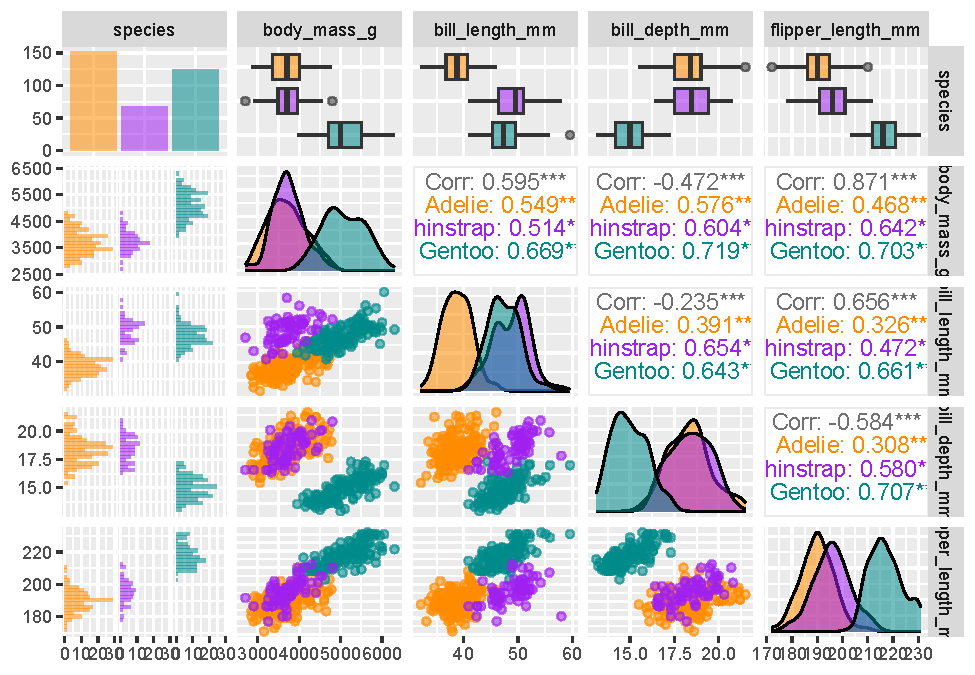
\includegraphics[width=0.9\linewidth]{EnvDataScience_files/figure-latex/unnamed-chunk-121-1} \end{center}

In this section, we'll explore visualization methods in R. Visualization has been a key element of R since its inception, since visualization is central to the exploratory philosophy of the language.

\section{plot in base R}\label{plot-in-base-r}

In this chapter, we'll spend a lot more time looking at \texttt{ggplot2} due to its clear syntax using the \emph{grammar of graphics}. However, the base R \texttt{plot} system generally does a good job of coming up with the most likely graphical output based on the data you provide, so we'll use it from time to time. Through the book you'll see various references to its use, including setting graphical parameters with \texttt{par}, such as the \texttt{cex} for defining the relative size of text characters and point symbols, \texttt{lty} and \texttt{lwd} for line type and width, and \emph{many} others. Users are encouraged to explore these with \texttt{?par} to learn about parameters (even things like creating multiple plots using \texttt{mfrow} as you can see in Figure \ref{fig:visFlipperLength}), and \texttt{?plot} to learn more overall about the generic X-Y plotting system.

\begin{Shaded}
\begin{Highlighting}[]
\FunctionTok{par}\NormalTok{(}\AttributeTok{mfrow=}\FunctionTok{c}\NormalTok{(}\DecValTok{1}\NormalTok{,}\DecValTok{2}\NormalTok{))}
\FunctionTok{plot}\NormalTok{(penguins}\SpecialCharTok{$}\NormalTok{body\_mass\_g, penguins}\SpecialCharTok{$}\NormalTok{flipper\_length\_mm,}
     \AttributeTok{cex=}\FloatTok{0.5}\NormalTok{) }\CommentTok{\# half{-}size point symbol}
\FunctionTok{plot}\NormalTok{(penguins}\SpecialCharTok{$}\NormalTok{species, penguins}\SpecialCharTok{$}\NormalTok{flipper\_length\_mm,}
     \AttributeTok{ylab=}\StringTok{"flipper length (mm)"}\NormalTok{,}
     \AttributeTok{xlab=}\StringTok{"species"}\NormalTok{)}
\end{Highlighting}
\end{Shaded}

\begin{figure}

{\centering 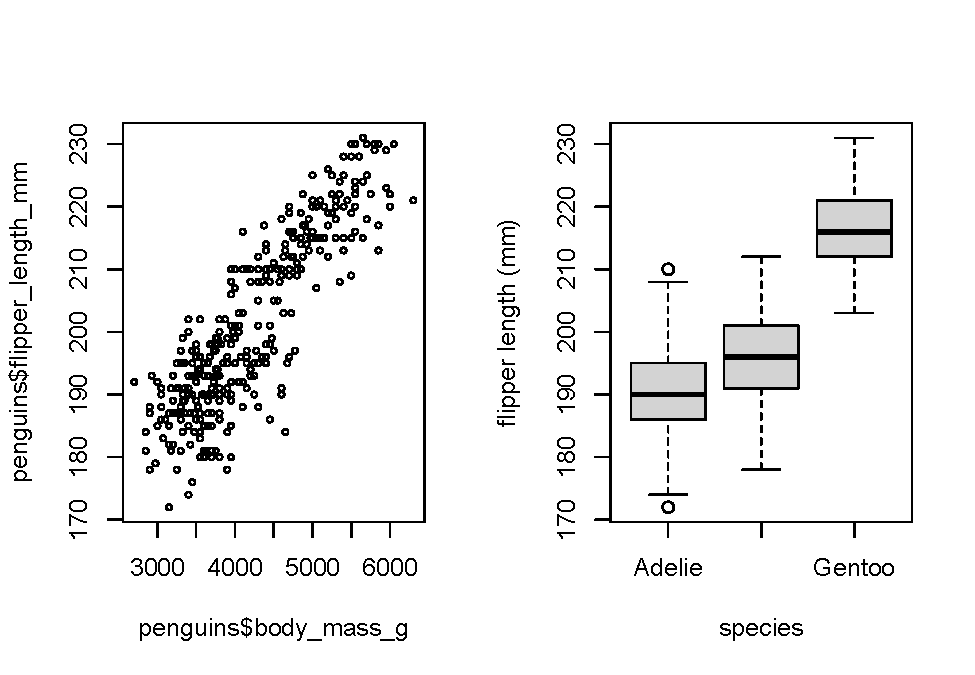
\includegraphics[width=1\linewidth]{EnvDataScience_files/figure-latex/visFlipperLength-1} 

}

\caption{Flipper length by mass and by species, base plot system. The Antarctic peninsula penguin data set is from @palmer.}\label{fig:visFlipperLength}
\end{figure}

\section{ggplot2}\label{ggplot2}

\index{ggplot2}We'll mostly focus however on gpplot2, based on the \emph{Grammar of Graphics} because it provides considerable control over your graphics while remaining fairly easily readable, as long as you buy into its grammar.

The \texttt{ggplot2} app (and its primary function \texttt{ggplot}) looks at three aspects of a graph:

\begin{itemize}
\tightlist
\item
  data : where are the data coming from?
\item
  geometry : what type of graph are we creating?
\item
  \index{aesthetics}aesthetics : what choices can we make about symbology and how do we connect symbology to data?
\end{itemize}

As with other tidyverse and RStudio packages, find the ggplot2 cheat sheet at \url{https://www.rstudio.com/resources/cheatsheets/}

\section{Plotting one variable}\label{plotting-one-variable}

The \texttt{ggplot} function provides plots of single and multiple variables, using various coordinate systems (including geographic). We'll start with just plotting one variable, which might be \emph{continuous} -- where we might want to see a histogram, density plot, or dot plot -- or \emph{discrete} -- where we might want to see something like a a bar graph, like the first example below (Figure \ref{fig:visSimpleBarGraph}).

We'll look at a study of Normalized Difference Vegetation Index from a transect across a montane meadow in the northern Sierra Nevada, derived from multispectral drone imagery (\citeproc{ref-NDVI}{Davis et al. 2020}).

\begin{Shaded}
\begin{Highlighting}[]
\FunctionTok{library}\NormalTok{(igisci)}
\FunctionTok{library}\NormalTok{(tidyverse)}
\FunctionTok{summary}\NormalTok{(XSptsNDVI)}
\end{Highlighting}
\end{Shaded}

\begin{verbatim}
##     DistNtoS       elevation        vegetation      geometry   NDVIgrowing    
##  Min.   :  0.0   Min.   :1510   Length   :29   Length   :29   Min.   :0.3255  
##  1st Qu.: 37.0   1st Qu.:1510   N.unique : 4   N.unique :29   1st Qu.:0.5052  
##  Median :175.0   Median :1511   N.blank  : 0   N.blank  : 0   Median :0.6169  
##  Mean   :164.7   Mean   :1511   Min.nchar: 4   Min.nchar:25   Mean   :0.5901  
##  3rd Qu.:275.5   3rd Qu.:1511   Max.nchar:15   Max.nchar:27   3rd Qu.:0.6768  
##  Max.   :298.8   Max.   :1511                                 Max.   :0.7683  
##  NDVIsenescent   
##  Min.   :0.1402  
##  1st Qu.:0.2418  
##  Median :0.2817  
##  Mean   :0.3662  
##  3rd Qu.:0.5407  
##  Max.   :0.7578
\end{verbatim}

\begin{Shaded}
\begin{Highlighting}[]
\FunctionTok{ggplot}\NormalTok{(XSptsNDVI, }\FunctionTok{aes}\NormalTok{(vegetation)) }\SpecialCharTok{+} 
  \FunctionTok{geom\_bar}\NormalTok{()}
\end{Highlighting}
\end{Shaded}

\begin{figure}

{\centering 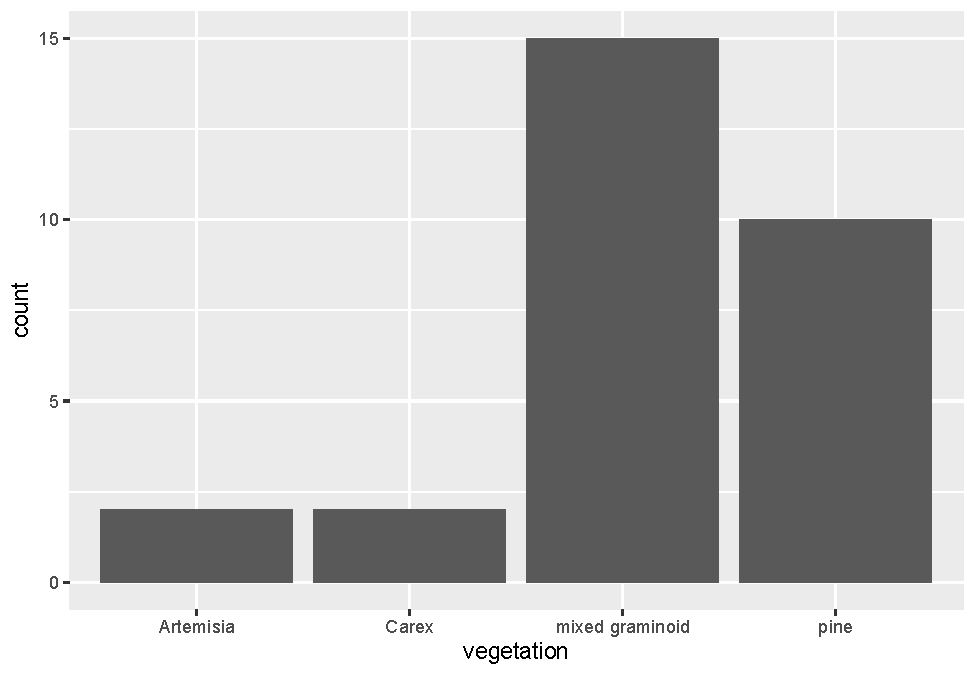
\includegraphics[width=0.75\linewidth]{EnvDataScience_files/figure-latex/visSimpleBarGraph-1} 

}

\caption{Simple bar graph of meadow vegetation samples}\label{fig:visSimpleBarGraph}
\end{figure}

\subsection{Histogram}\label{histogram}

\index{histogram}Histograms are very useful for looking at the distribution of continuous variables (Figure \ref{fig:visNDVIknuthson}). We'll start by using a pivot table (these will be discussed in the next chapter, on data transformation.)

\begin{Shaded}
\begin{Highlighting}[]
\NormalTok{XSptsPheno }\OtherTok{\textless{}{-}}\NormalTok{ XSptsNDVI }\SpecialCharTok{\%\textgreater{}\%}
  \FunctionTok{filter}\NormalTok{(vegetation }\SpecialCharTok{!=} \StringTok{"pine"}\NormalTok{) }\SpecialCharTok{\%\textgreater{}\%}
  \FunctionTok{pivot\_longer}\NormalTok{(}\AttributeTok{cols =} \FunctionTok{starts\_with}\NormalTok{(}\StringTok{"NDVI"}\NormalTok{), }
               \AttributeTok{names\_to =} \StringTok{"phenology"}\NormalTok{, }
               \AttributeTok{values\_to =} \StringTok{"NDVI"}\NormalTok{) }\SpecialCharTok{\%\textgreater{}\%}
  \FunctionTok{mutate}\NormalTok{(}\AttributeTok{phenology =} \FunctionTok{str\_sub}\NormalTok{(phenology, }\DecValTok{5}\NormalTok{, }\FunctionTok{str\_length}\NormalTok{(phenology)))}
\end{Highlighting}
\end{Shaded}

\begin{Shaded}
\begin{Highlighting}[]
\NormalTok{XSptsPheno }\SpecialCharTok{\%\textgreater{}\%}
  \FunctionTok{ggplot}\NormalTok{(}\FunctionTok{aes}\NormalTok{(NDVI)) }\SpecialCharTok{+} 
  \FunctionTok{geom\_histogram}\NormalTok{(}\AttributeTok{binwidth=}\FloatTok{0.05}\NormalTok{)}
\end{Highlighting}
\end{Shaded}

\begin{figure}

{\centering 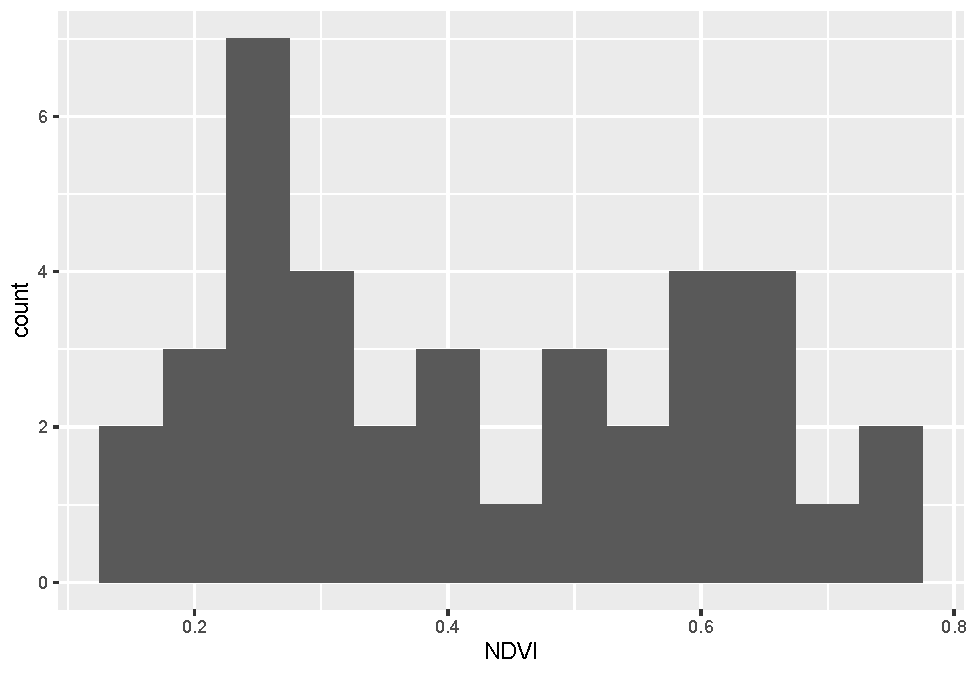
\includegraphics[width=0.75\linewidth]{EnvDataScience_files/figure-latex/visNDVIknuthson-1} 

}

\caption{Distribution of NDVI, Knuthson Meadow}\label{fig:visNDVIknuthson}
\end{figure}

Histograms can be created in a couple of ways, one the conventional histogram that provides the most familiar view, for instance of the ``bell curve'' of a normal distribution (Figure \ref{fig:visTemperaturesHisto}).

\begin{Shaded}
\begin{Highlighting}[]
\NormalTok{sierraData }\SpecialCharTok{\%\textgreater{}\%}
    \FunctionTok{ggplot}\NormalTok{(}\FunctionTok{aes}\NormalTok{(TEMPERATURE)) }\SpecialCharTok{+}
  \FunctionTok{geom\_histogram}\NormalTok{(}\AttributeTok{fill=}\StringTok{"dark green"}\NormalTok{)}
\end{Highlighting}
\end{Shaded}

\begin{figure}

{\centering 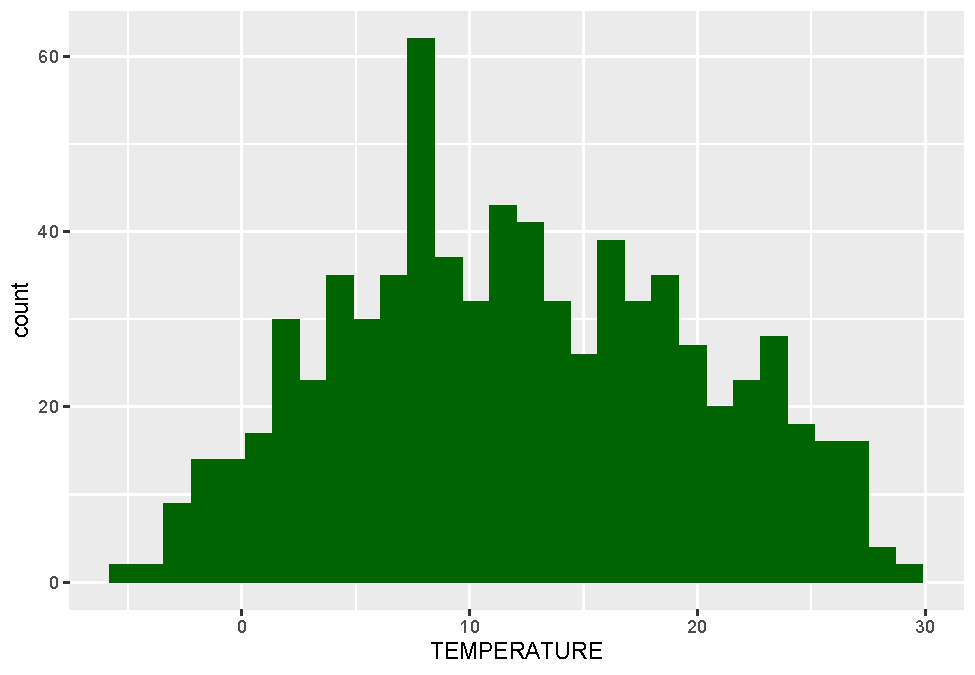
\includegraphics[width=0.75\linewidth]{EnvDataScience_files/figure-latex/visTemperaturesHisto-1} 

}

\caption{Distribution of Average Monthly Temperatures, Sierra Nevada}\label{fig:visTemperaturesHisto}
\end{figure}

Alternatively, we can look at a \index{histogram, cumulative}\emph{cumulative} histogram, which makes it easier to see percentiles and the median (50th percentile), by using the \texttt{cumsum()} function (Figure \ref{fig:visCumHisto}).

\begin{Shaded}
\begin{Highlighting}[]
\NormalTok{n }\OtherTok{\textless{}{-}} \FunctionTok{length}\NormalTok{(sierraData}\SpecialCharTok{$}\NormalTok{TEMPERATURE)}
\NormalTok{sierraData }\SpecialCharTok{\%\textgreater{}\%}
  \FunctionTok{ggplot}\NormalTok{(}\FunctionTok{aes}\NormalTok{(TEMPERATURE)) }\SpecialCharTok{+}
  \FunctionTok{geom\_histogram}\NormalTok{(}\FunctionTok{aes}\NormalTok{(}\AttributeTok{y=}\FunctionTok{cumsum}\NormalTok{(..count..)}\SpecialCharTok{/}\NormalTok{n), }\AttributeTok{fill=}\StringTok{"dark goldenrod"}\NormalTok{)}
\end{Highlighting}
\end{Shaded}

\begin{figure}

{\centering 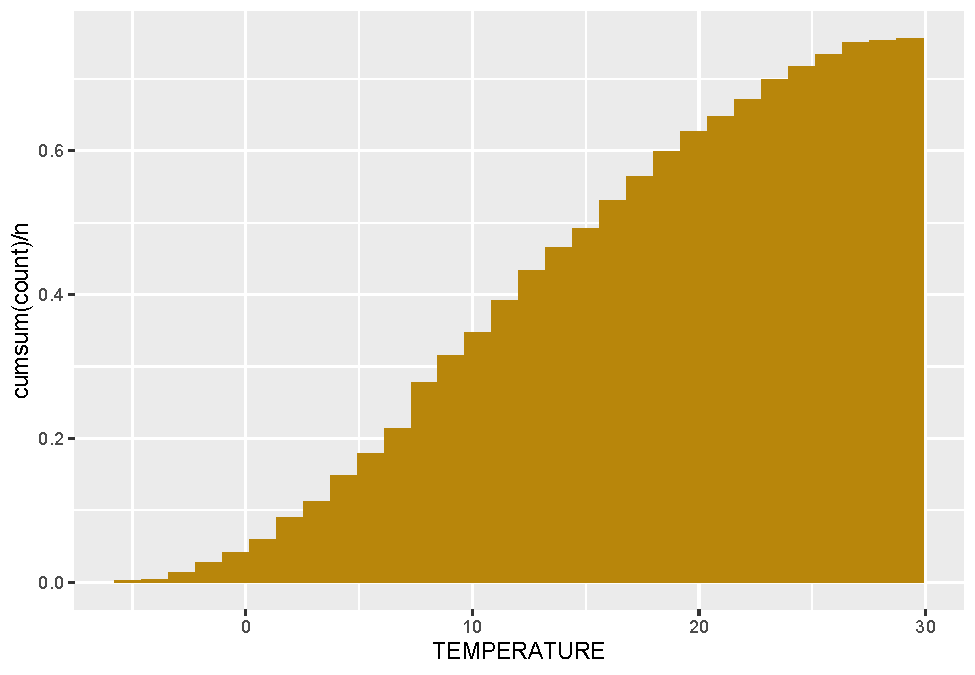
\includegraphics[width=0.75\linewidth]{EnvDataScience_files/figure-latex/visCumHisto-1} 

}

\caption{Cumulative Distribution of Average Monthly Temperatures, Sierra Nevada}\label{fig:visCumHisto}
\end{figure}

\subsubsection{Building a histogram from a time series}\label{building-a-histogram-from-a-time-series}

If we want to work with a time series, we can start by converting it to a tibble, and meanwhile providing a more explanatory variable name.

\begin{Shaded}
\begin{Highlighting}[]
\NormalTok{NileT }\OtherTok{=} \FunctionTok{tibble}\NormalTok{(}\AttributeTok{AnnualFlow=}\NormalTok{Nile)}
\FunctionTok{ggplot}\NormalTok{(}\AttributeTok{data=}\NormalTok{NileT, }\FunctionTok{aes}\NormalTok{(}\AttributeTok{x=}\NormalTok{AnnualFlow)) }\SpecialCharTok{+}
  \FunctionTok{geom\_histogram}\NormalTok{(}\AttributeTok{binwidth=}\DecValTok{20}\NormalTok{)}
\end{Highlighting}
\end{Shaded}

\begin{center}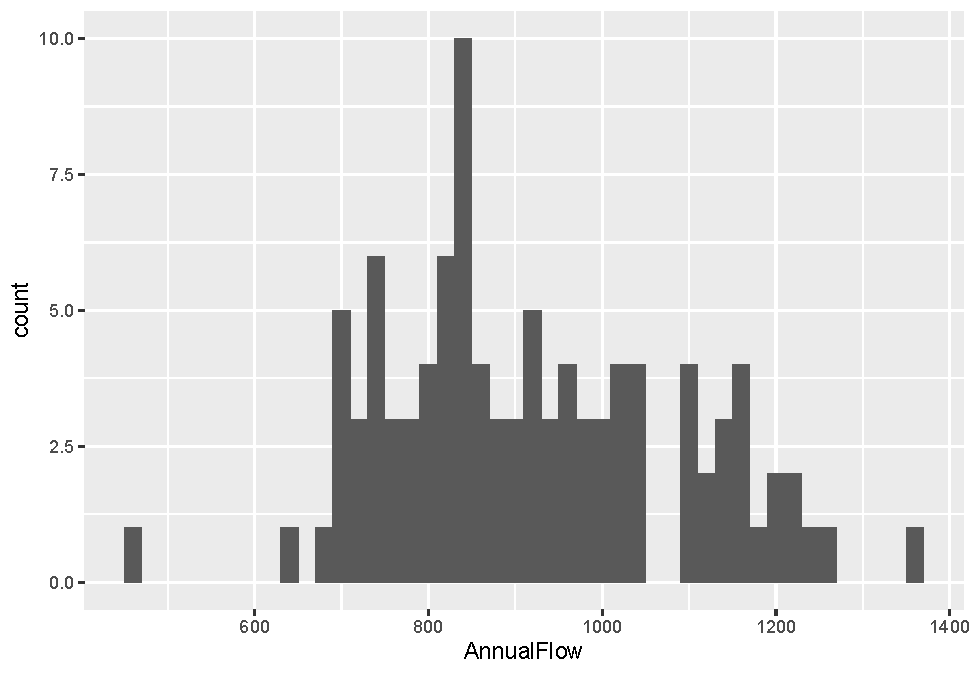
\includegraphics[width=0.75\linewidth]{EnvDataScience_files/figure-latex/nileFlow-1} \end{center}

\begin{quote}
To learn more about built-in data like time series, you can simply use the console help method like you would learn about a function. So try entering \texttt{?Nile}.
\end{quote}

\subsection{Density plot}\label{density-plot}

\index{density plot}Density represents how much of the distribution we have out of the total. The total area (sum of widths of bins times densities of that bin) adds up to 1. We'll use a density plot to looking at our NDVI data again (Figure \ref{fig:visDensNDVI}).

\begin{Shaded}
\begin{Highlighting}[]
\NormalTok{XSptsPheno }\SpecialCharTok{\%\textgreater{}\%} 
  \FunctionTok{ggplot}\NormalTok{(}\FunctionTok{aes}\NormalTok{(NDVI)) }\SpecialCharTok{+} 
  \FunctionTok{geom\_density}\NormalTok{()}
\end{Highlighting}
\end{Shaded}

\begin{figure}

{\centering 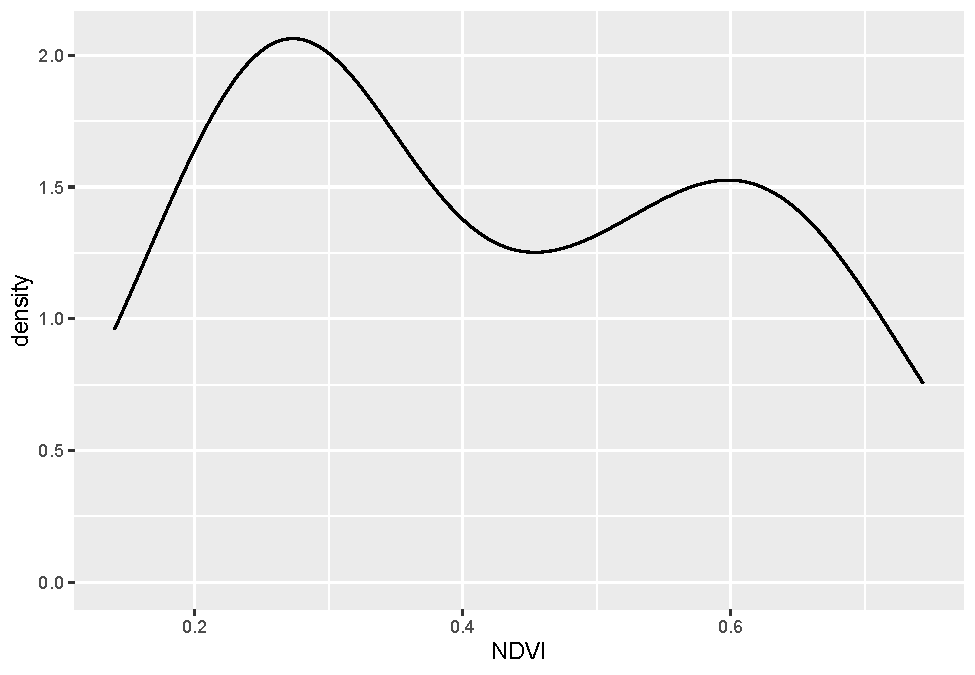
\includegraphics[width=0.75\linewidth]{EnvDataScience_files/figure-latex/visDensNDVI-1} 

}

\caption{Density plot of NDVI, Knuthson Meadow}\label{fig:visDensNDVI}
\end{figure}

\begin{quote}
Note that NDVI values are \textless1 so bins are very small numbers, so in this case densities can be \textgreater1.
\end{quote}

To communicate more information, we might want to use color and \index{alpha}transparency (alpha) settings. The following graph (Figure \ref{fig:visDensityAlpha}) will separate the data by phenology (``growing'' vs.~``senescence'' seasons) using color, and use the alpha setting to allow these overlapping distributions to both be seen. To do this, we'll:

\begin{itemize}
\tightlist
\item
  ``map'' a variable (phenology) to an aesthetic property (fill color of the density polygon)
\item
  set a a property (alpha = 0.2) to all polygons of the density plot. The alpha channel of colors defines its opacity, from invisible (0) to opaque (1) so is commonly used to set as its reverse, transparency.
\end{itemize}

\begin{Shaded}
\begin{Highlighting}[]
\NormalTok{XSptsPheno }\SpecialCharTok{\%\textgreater{}\%}
  \FunctionTok{ggplot}\NormalTok{(}\FunctionTok{aes}\NormalTok{(NDVI, }\AttributeTok{fill=}\NormalTok{phenology)) }\SpecialCharTok{+}
  \FunctionTok{geom\_density}\NormalTok{(}\AttributeTok{alpha=}\FloatTok{0.2}\NormalTok{)}
\end{Highlighting}
\end{Shaded}

\begin{figure}

{\centering 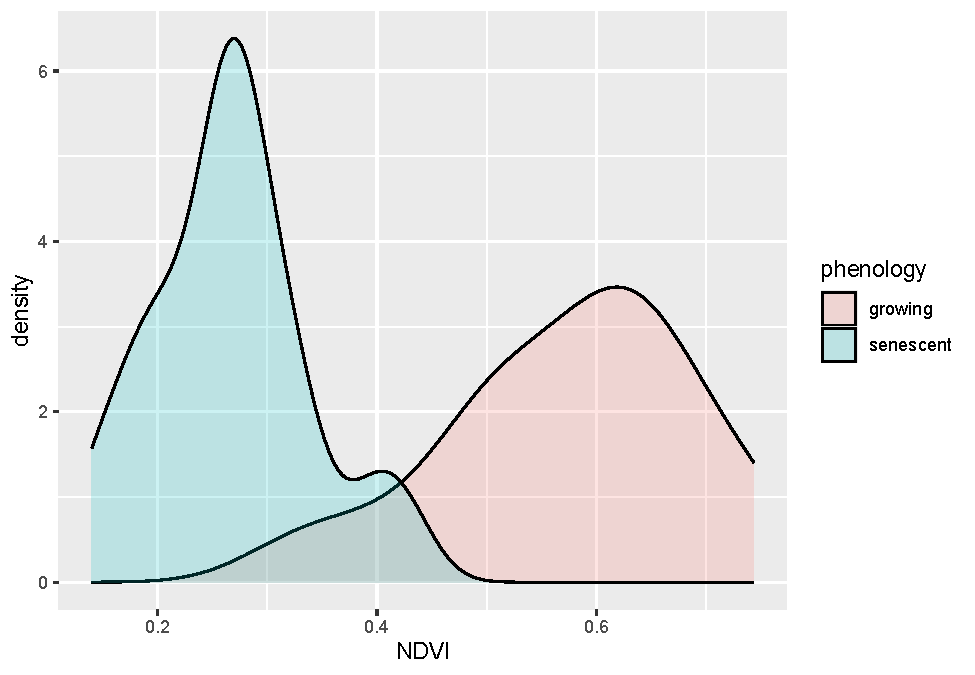
\includegraphics[width=0.75\linewidth]{EnvDataScience_files/figure-latex/visDensityAlpha-1} 

}

\caption{Comparative density plot using alpha setting}\label{fig:visDensityAlpha}
\end{figure}

\begin{quote}
Why is the color called \index{fill}\textbf{fill}? For polygons, ``color'' is used for the boundary.
\end{quote}

Similarly for the eucalyptus and oak study, we can overlay the two distributions (Figure \ref{fig:visRunoffEucOak}). Since the two distributions overlap considerably, the benefit of the alpha settings is clear.

\begin{Shaded}
\begin{Highlighting}[]
\NormalTok{tidy\_eucoak }\SpecialCharTok{\%\textgreater{}\%}
  \FunctionTok{ggplot}\NormalTok{(}\FunctionTok{aes}\NormalTok{(}\FunctionTok{log}\NormalTok{(runoff\_L),}\AttributeTok{fill=}\NormalTok{tree)) }\SpecialCharTok{+}
  \FunctionTok{geom\_density}\NormalTok{(}\AttributeTok{alpha=}\FloatTok{0.2}\NormalTok{)}
\end{Highlighting}
\end{Shaded}

\begin{figure}

{\centering 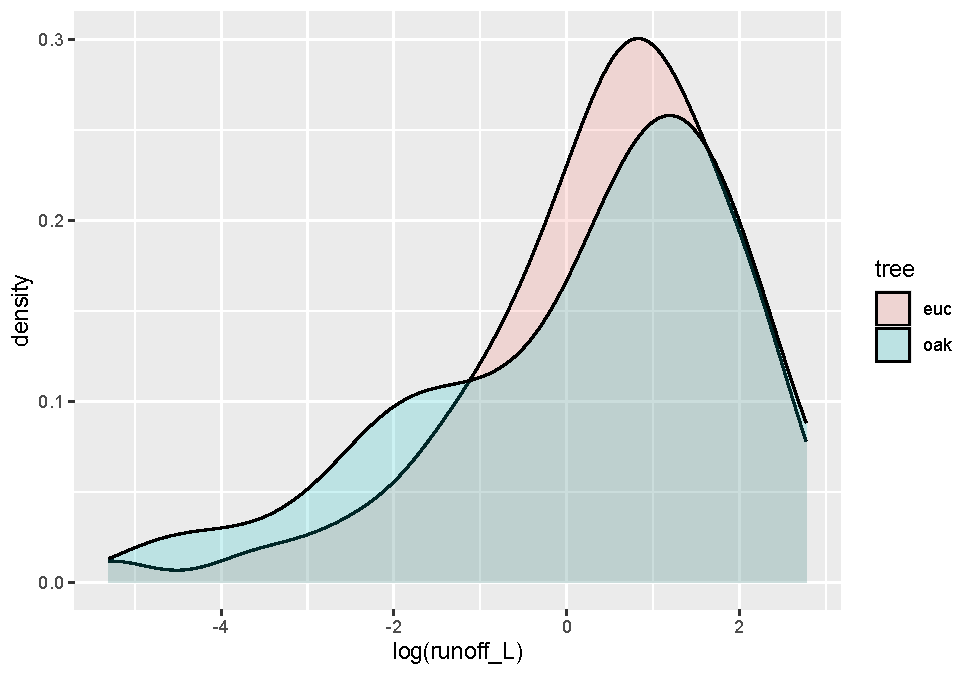
\includegraphics[width=0.75\linewidth]{EnvDataScience_files/figure-latex/visRunoffEucOak-1} 

}

\caption{Runoff under eucalyptus and oak in Bay Area sites}\label{fig:visRunoffEucOak}
\end{figure}

\subsection{Boxplot}\label{boxplot}

Tukey \index{boxplot}boxplots provide another way of looking at the distributions of continuous variables. Typically these are stratified by a factor, such as \texttt{site} in the euc/oak study (Figure \ref{fig:visBoxplotByRunoff}):

\begin{Shaded}
\begin{Highlighting}[]
\FunctionTok{ggplot}\NormalTok{(}\AttributeTok{data =}\NormalTok{ tidy\_eucoak) }\SpecialCharTok{+}
  \FunctionTok{geom\_boxplot}\NormalTok{(}\FunctionTok{aes}\NormalTok{(}\AttributeTok{x =}\NormalTok{ site, }\AttributeTok{y =}\NormalTok{ runoff\_L))}
\end{Highlighting}
\end{Shaded}

\begin{figure}

{\centering 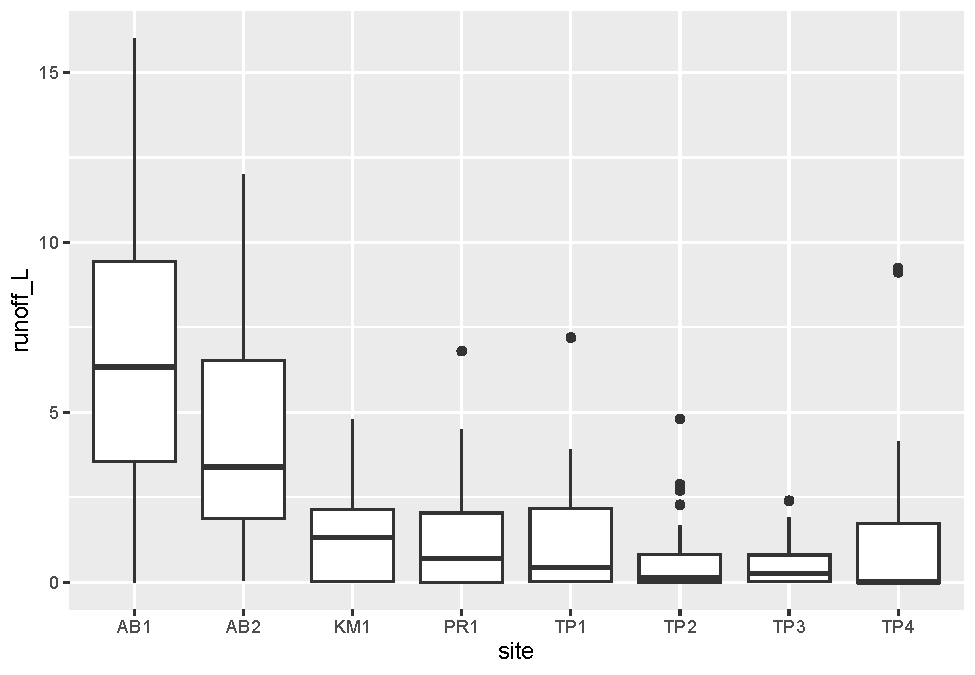
\includegraphics[width=0.75\linewidth]{EnvDataScience_files/figure-latex/visBoxplotByRunoff-1} 

}

\caption{Boxplot of runoff by site}\label{fig:visBoxplotByRunoff}
\end{figure}

And then as we did above, we can communicate more by coloring by tree type. Note that this is called \emph{within} the \index{aes}\texttt{aes()} function (Figure \ref{fig:visEucOakRunoffColored}).

\begin{Shaded}
\begin{Highlighting}[]
\FunctionTok{ggplot}\NormalTok{(}\AttributeTok{data =}\NormalTok{ tidy\_eucoak) }\SpecialCharTok{+}
  \FunctionTok{geom\_boxplot}\NormalTok{(}\FunctionTok{aes}\NormalTok{(}\AttributeTok{x=}\NormalTok{site, }\AttributeTok{y=}\NormalTok{runoff\_L, }\AttributeTok{color=}\NormalTok{tree))}
\end{Highlighting}
\end{Shaded}

\begin{figure}

{\centering 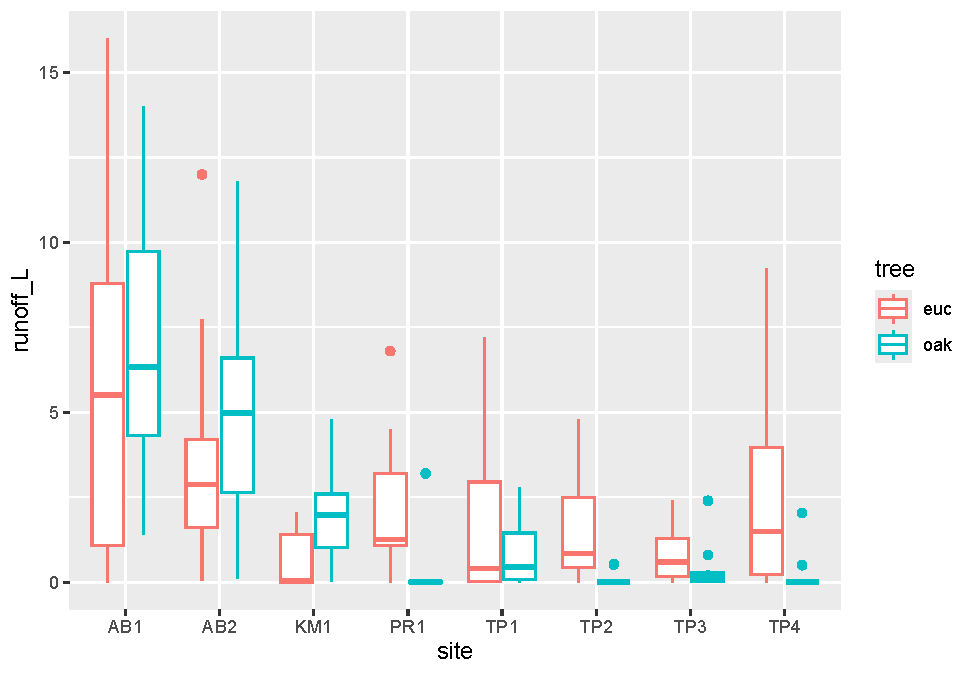
\includegraphics[width=0.75\linewidth]{EnvDataScience_files/figure-latex/visEucOakRunoffColored-1} 

}

\caption{Runoff at Bay Area Sites, colored as eucalyptus and oak}\label{fig:visEucOakRunoffColored}
\end{figure}

\textbf{Visualizing soil CO\textsubscript{2} data with a box plot}

In a study of soil CO\textsubscript{2} in the \index{Marble Mountains}Marble Mountains of California (\citeproc{ref-marblesCO2}{Davis et al. 2001}), we sampled extracted soil air (Figure \ref{fig:visSoilGasSampling}) in a 11-point transect across Marble Valley in 1997 (Figure \ref{fig:visMarblesSitesTopo}). Again, a Tukey boxplot is useful for visualization (Figure \ref{fig:visSoilTukey}).

\begin{quote}
Note that in this book you'll often see CO\textsubscript{2} written as CO2. These are both meant to refer to carbon dioxide, but I've learned that subscripts in figure headings don't always get passed through to the LaTeX compiler for the pdf/printed version, so I'm forced to write it without the subscript. Similarly CH\textsubscript{4} might be written as CH4, etc. The same applies often to variable names and axis labels in graphs, though there are some workarounds.
\end{quote}

\begin{figure}

{\centering 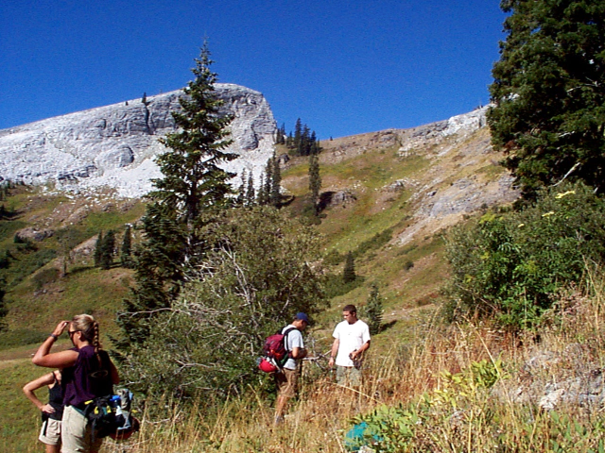
\includegraphics[width=0.75\linewidth]{img/marbleGap} 

}

\caption{Marble Valley, Marble Mountains Wilderness, California}\label{fig:visSoilGasSampling}
\end{figure}

\begin{figure}

{\centering 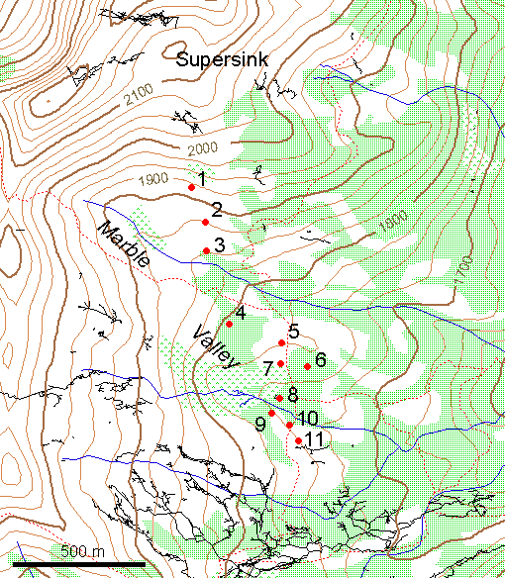
\includegraphics[width=0.5\linewidth]{img/marblesCO2map} 

}

\caption{Marble Mountains soil gas sampling sites, with surface topographic features and cave passages}\label{fig:visMarblesSitesTopo}
\end{figure}

\begin{Shaded}
\begin{Highlighting}[]
\NormalTok{soilCO2 }\OtherTok{\textless{}{-}}\NormalTok{ soilCO2\_97}
\NormalTok{soilCO2}\SpecialCharTok{$}\NormalTok{SITE }\OtherTok{\textless{}{-}} \FunctionTok{factor}\NormalTok{(soilCO2}\SpecialCharTok{$}\NormalTok{SITE)  }\CommentTok{\# in order to make the numeric field a factor}
\FunctionTok{ggplot}\NormalTok{(}\AttributeTok{data =}\NormalTok{ soilCO2, }\AttributeTok{mapping =} \FunctionTok{aes}\NormalTok{(}\AttributeTok{x =}\NormalTok{ SITE, }\AttributeTok{y =}\NormalTok{ CO2pct)) }\SpecialCharTok{+}
  \FunctionTok{geom\_boxplot}\NormalTok{()}
\end{Highlighting}
\end{Shaded}

\begin{figure}

{\centering 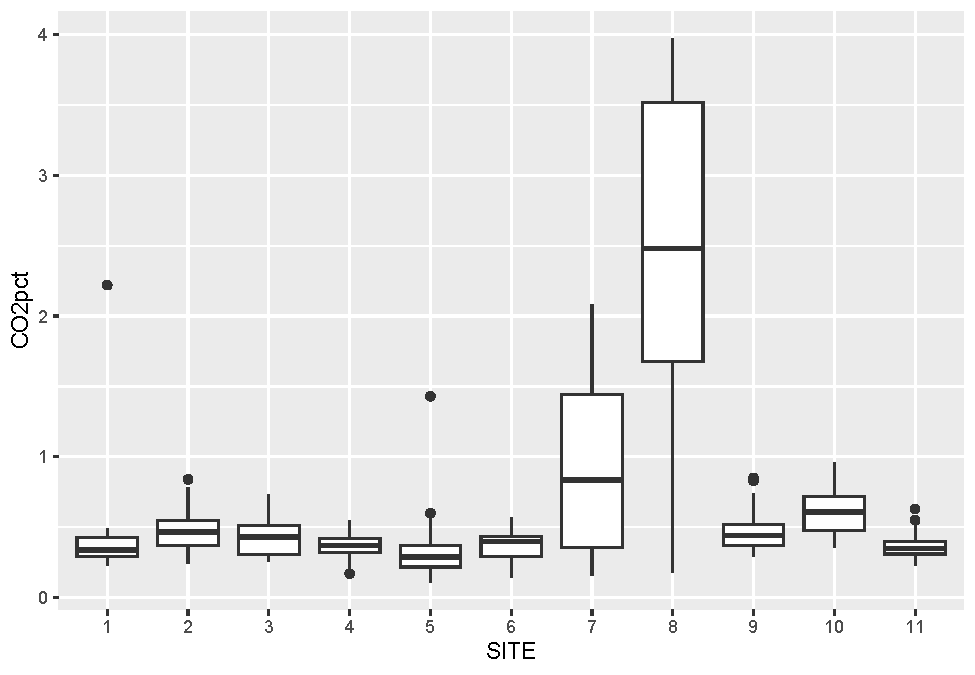
\includegraphics[width=0.75\linewidth]{EnvDataScience_files/figure-latex/visSoilTukey-1} 

}

\caption{Visualizing soil CO2 data with a Tukey box plot}\label{fig:visSoilTukey}
\end{figure}

\section{Plotting Two Variables}\label{plotting-two-variables}

\subsection{Two continuous variables}\label{two-continuous-variables}

\index{continuous variables}We've looked at this before -- the scatterplot -- but let's try some new data: daily discharge (Q) and other data (like EC, electrical conductivity, a surrogate for solute concentration) from Sagehen Creek, north of Truckee, CA, 1970 to present. I downloaded the data for this location (which I've visited multiple times to chat with the USGS hydrologist about calibration methods with my Sierra Nevada Field Campus students) from the \url{https://waterdata.usgs.gov/nwis/sw} site (Figure \ref{fig:visSagehenScatterplot}). If you visit this site, you can download similar data from thousands of surface water (as well as groundwater) gauges around the country.

\begin{Shaded}
\begin{Highlighting}[]
\FunctionTok{library}\NormalTok{(tidyverse); }\FunctionTok{library}\NormalTok{(lubridate); }\FunctionTok{library}\NormalTok{(igisci)}
\NormalTok{sagehen }\OtherTok{\textless{}{-}} \FunctionTok{read\_csv}\NormalTok{(}\FunctionTok{ex}\NormalTok{(}\StringTok{"sierra/sagehen\_dv.csv"}\NormalTok{))}
\FunctionTok{plot}\NormalTok{(sagehen}\SpecialCharTok{$}\NormalTok{Q,sagehen}\SpecialCharTok{$}\NormalTok{EC)}
\end{Highlighting}
\end{Shaded}

\begin{figure}

{\centering 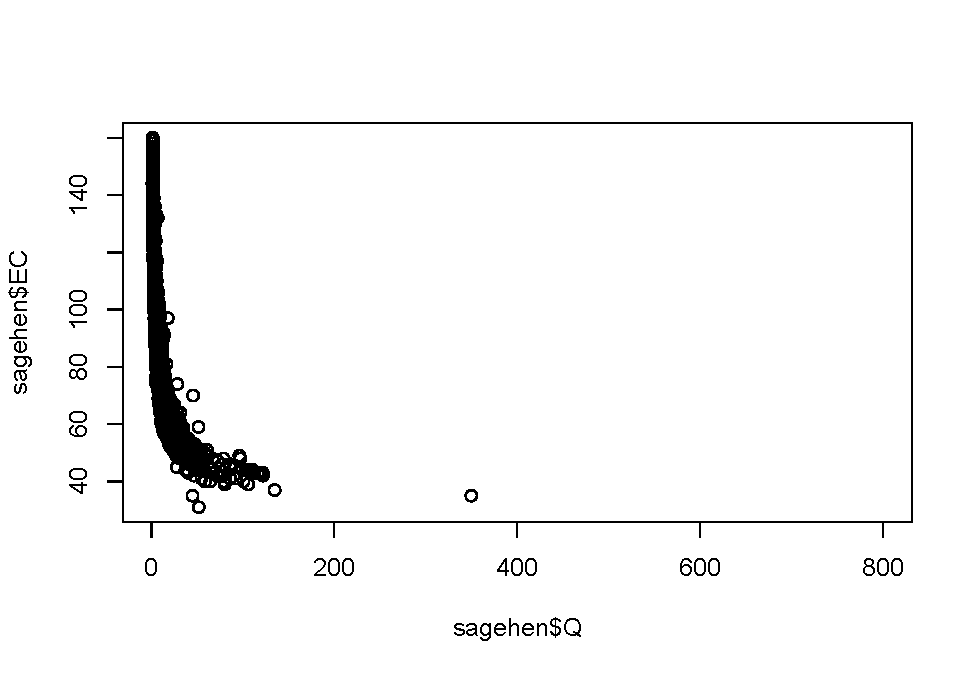
\includegraphics[width=0.75\linewidth]{EnvDataScience_files/figure-latex/visSagehenScatterplot-1} 

}

\caption{Scatter plot of discharge (Q) and specific electrical conductance (EC) for Sagehen Creek, California}\label{fig:visSagehenScatterplot}
\end{figure}

\index{streamflow}Streamflow and \index{water quality}water quality are commonly best represented using a log transform, or we can just use log scaling, which retains the original units (Figure \ref{fig:visSagehenQEClog10}).

\begin{Shaded}
\begin{Highlighting}[]
\FunctionTok{ggplot}\NormalTok{(}\AttributeTok{data=}\NormalTok{sagehen, }\FunctionTok{aes}\NormalTok{(}\AttributeTok{x=}\NormalTok{Q, }\AttributeTok{y=}\NormalTok{EC)) }\SpecialCharTok{+} \FunctionTok{geom\_point}\NormalTok{() }\SpecialCharTok{+}
  \FunctionTok{scale\_x\_log10}\NormalTok{() }\SpecialCharTok{+} \FunctionTok{scale\_y\_log10}\NormalTok{()}
\end{Highlighting}
\end{Shaded}

\begin{figure}

{\centering 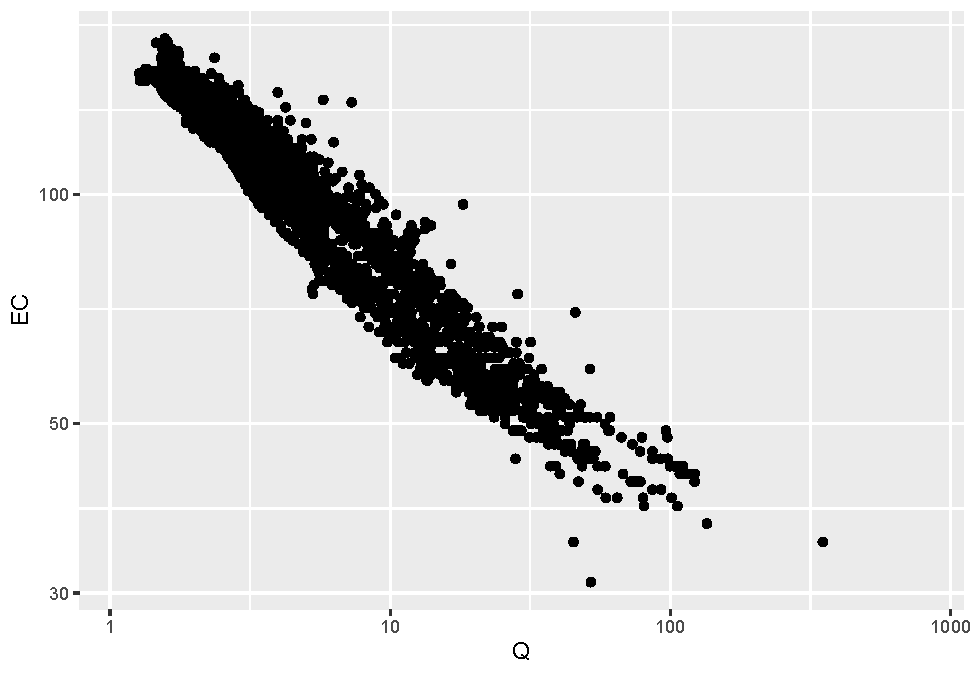
\includegraphics[width=0.75\linewidth]{EnvDataScience_files/figure-latex/visSagehenQEClog10-1} 

}

\caption{Q and EC for Sagehen Creek, using log10 scaling on both axes}\label{fig:visSagehenQEClog10}
\end{figure}

\begin{itemize}
\tightlist
\item
  For both graphs, the \texttt{aes} (``aesthetics'') function specifies the variables to use as x and y coordinates
\item
  geom\_point creates a scatter plot of those coordinate points
\end{itemize}

\textbf{Set color for all (\emph{not} in \texttt{aes()})}

\index{color for all symbols}Sometimes all you want is a simple graph with one color for all points (Figure \ref{fig:visOneColor}). Note that:

\begin{itemize}
\tightlist
\item
  color is defined outside of \texttt{aes}, so it applies to all points.
\item
  mapping is first argument of \texttt{geom\_point}, so \texttt{mapping\ =} is not needed.
\end{itemize}

\begin{Shaded}
\begin{Highlighting}[]
\FunctionTok{ggplot}\NormalTok{(}\AttributeTok{data=}\NormalTok{sierraFeb) }\SpecialCharTok{+} 
  \FunctionTok{geom\_point}\NormalTok{(}\FunctionTok{aes}\NormalTok{(TEMPERATURE, ELEVATION), }\AttributeTok{color=}\StringTok{"blue"}\NormalTok{)}
\end{Highlighting}
\end{Shaded}

\begin{figure}

{\centering 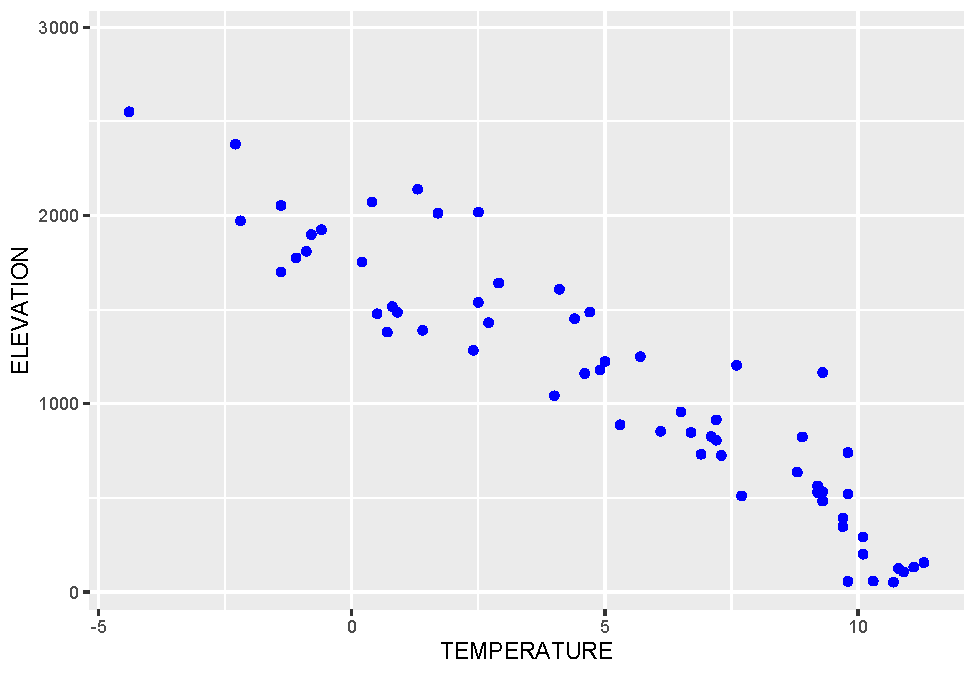
\includegraphics[width=0.75\linewidth]{EnvDataScience_files/figure-latex/visOneColor-1} 

}

\caption{Setting one color for all points}\label{fig:visOneColor}
\end{figure}

\subsection{Two variables, one discrete}\label{two-variables-one-discrete}

\index{discrete variable}We've already looked at bringing in a factor to a histogram and a boxplot, but there's the even simpler bar graph that does this, if we're just interested in comparing values. This graph compares runoff by site (Figure \ref{fig:vis2var1discrete}).

\begin{Shaded}
\begin{Highlighting}[]
\FunctionTok{ggplot}\NormalTok{(tidy\_eucoak) }\SpecialCharTok{+}
  \FunctionTok{geom\_bar}\NormalTok{(}\FunctionTok{aes}\NormalTok{(site, runoff\_L), }\AttributeTok{stat=}\StringTok{"identity"}\NormalTok{)}
\end{Highlighting}
\end{Shaded}

\begin{figure}

{\centering 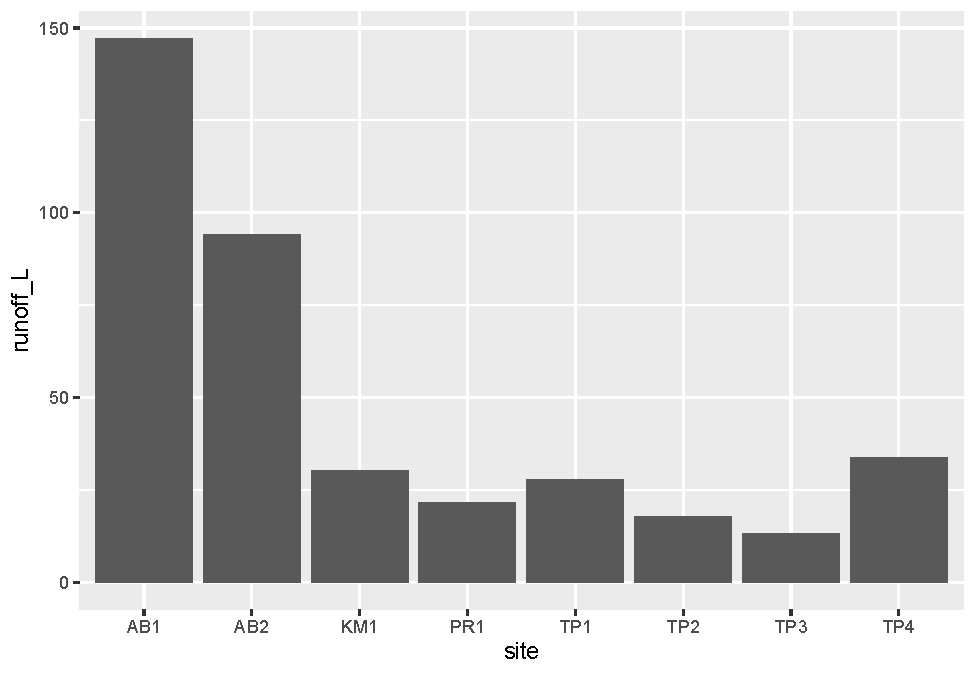
\includegraphics[width=0.75\linewidth]{EnvDataScience_files/figure-latex/vis2var1discrete-1} 

}

\caption{Two variables, one discrete}\label{fig:vis2var1discrete}
\end{figure}

\begin{quote}
Note that we also used the \texttt{geom\_bar} graph earlier for a single discrete variable, but instead of displaying a continuous variable like runoff, it just displayed the count (frequency) of observations, so was a type of histogram.
\end{quote}

\subsection{Color systems}\label{color-systems}

\index{color systems}There's a lot to working with color, with different color schemes needed for continuous data vs discrete values, and situations like bidirectional data. We'll look into some basics, but the reader is recommended to learn more at sources like \url{https://cran.r-project.org/web/packages/RColorBrewer/index.html} or \url{https://colorbrewer2.org/} or just Googling ``rcolorbrewer'' or ``colorbrewer'' or even ``R colors''.

\subsubsection{Specifying colors to use for a graphical element}\label{specifying-colors-to-use-for-a-graphical-element}

When a color is requested for an entire graphical element, like geom\_point or geom\_line, and \emph{not} in the aesthetics, all feature get that color. In the following graph the same x and y values are used to display as points in blue and as lines in red (Figure \ref{fig:visAestheticsPtsLines}).

\begin{Shaded}
\begin{Highlighting}[]
\NormalTok{sierraFeb }\SpecialCharTok{\%\textgreater{}\%}
  \FunctionTok{ggplot}\NormalTok{(}\FunctionTok{aes}\NormalTok{(TEMPERATURE,ELEVATION)) }\SpecialCharTok{+}
  \FunctionTok{geom\_point}\NormalTok{(}\AttributeTok{color=}\StringTok{"blue"}\NormalTok{) }\SpecialCharTok{+}
  \FunctionTok{geom\_line}\NormalTok{(}\AttributeTok{color=}\StringTok{"red"}\NormalTok{)}
\end{Highlighting}
\end{Shaded}

\begin{figure}

{\centering 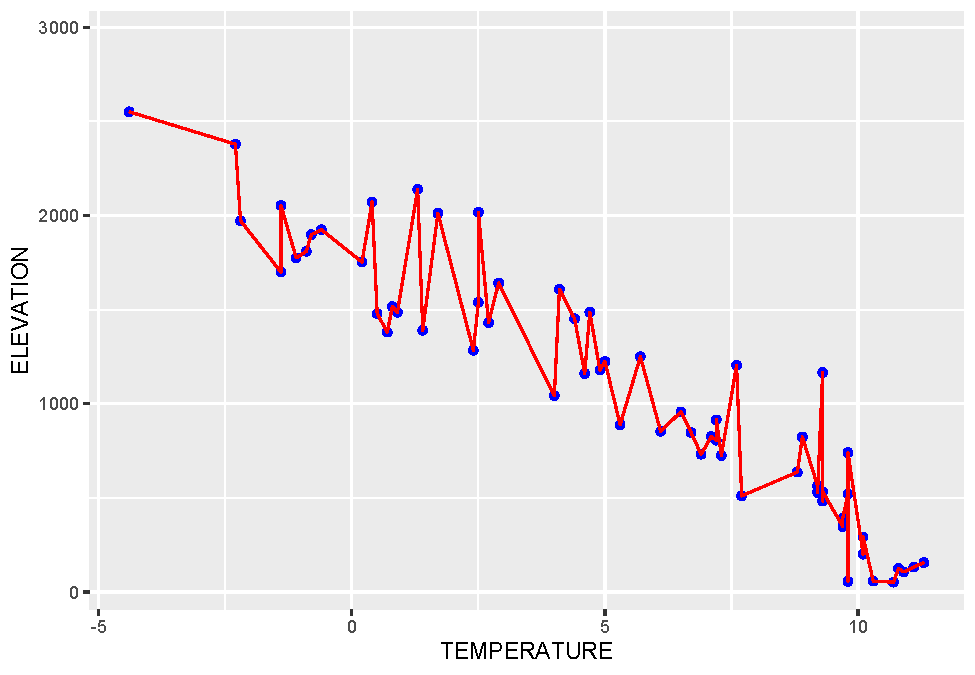
\includegraphics[width=0.75\linewidth]{EnvDataScience_files/figure-latex/visAestheticsPtsLines-1} 

}

\caption{Using aesthetics settings for both points and lines}\label{fig:visAestheticsPtsLines}
\end{figure}

\begin{quote}
Note the use of pipe to start with the data then apply ggplot. This is one approach for creating graphs, and provides a fairly straightforward way to progress from data to visualization.
\end{quote}

\subsubsection{Color from variable, in aesthetics}\label{color-from-variable-in-aesthetics}

\index{aesthetics}\index{color from variable}If color is connected to a variable within the \texttt{aes()} call, a color scheme is chosen to assign either a range (for continuous) or a set of unique colors (for discrete). In this graph, color is defined inside \texttt{aes}, so is based on COUNTY (Figure \ref{fig:visColorFromVar}).

\begin{Shaded}
\begin{Highlighting}[]
\FunctionTok{ggplot}\NormalTok{(}\AttributeTok{data=}\NormalTok{sierraFeb) }\SpecialCharTok{+} 
  \FunctionTok{geom\_point}\NormalTok{(}\FunctionTok{aes}\NormalTok{(TEMPERATURE, ELEVATION, }\AttributeTok{color=}\NormalTok{COUNTY))}
\end{Highlighting}
\end{Shaded}

\begin{figure}

{\centering 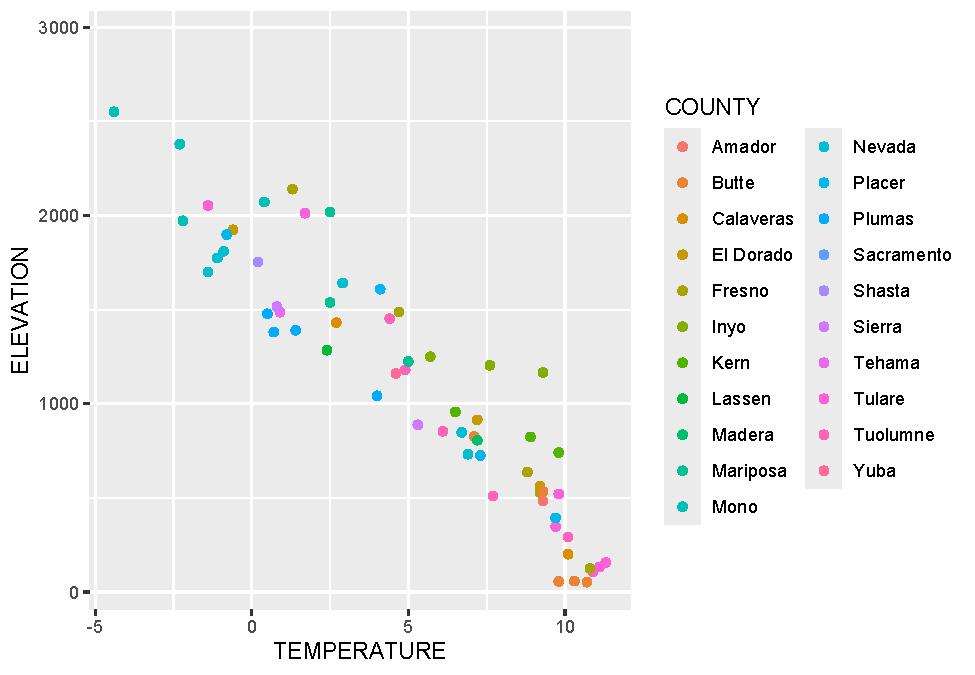
\includegraphics[width=0.75\linewidth]{EnvDataScience_files/figure-latex/visColorFromVar-1} 

}

\caption{Color set within aes()}\label{fig:visColorFromVar}
\end{figure}

Note that counties represent discrete data, and this is detected by ggplot to assign an appropriate color scheme. Continuous data will require a different palette (Figure \ref{fig:visSagehenQECcolorTemp}).

\begin{Shaded}
\begin{Highlighting}[]
\FunctionTok{ggplot}\NormalTok{(}\AttributeTok{data=}\NormalTok{sagehen, }\FunctionTok{aes}\NormalTok{(}\AttributeTok{x=}\NormalTok{Q, }\AttributeTok{y=}\NormalTok{EC, }\AttributeTok{col=}\NormalTok{waterTmax)) }\SpecialCharTok{+} \FunctionTok{geom\_point}\NormalTok{() }\SpecialCharTok{+}
  \FunctionTok{scale\_x\_log10}\NormalTok{() }\SpecialCharTok{+} \FunctionTok{scale\_y\_log10}\NormalTok{()}
\end{Highlighting}
\end{Shaded}

\begin{figure}

{\centering 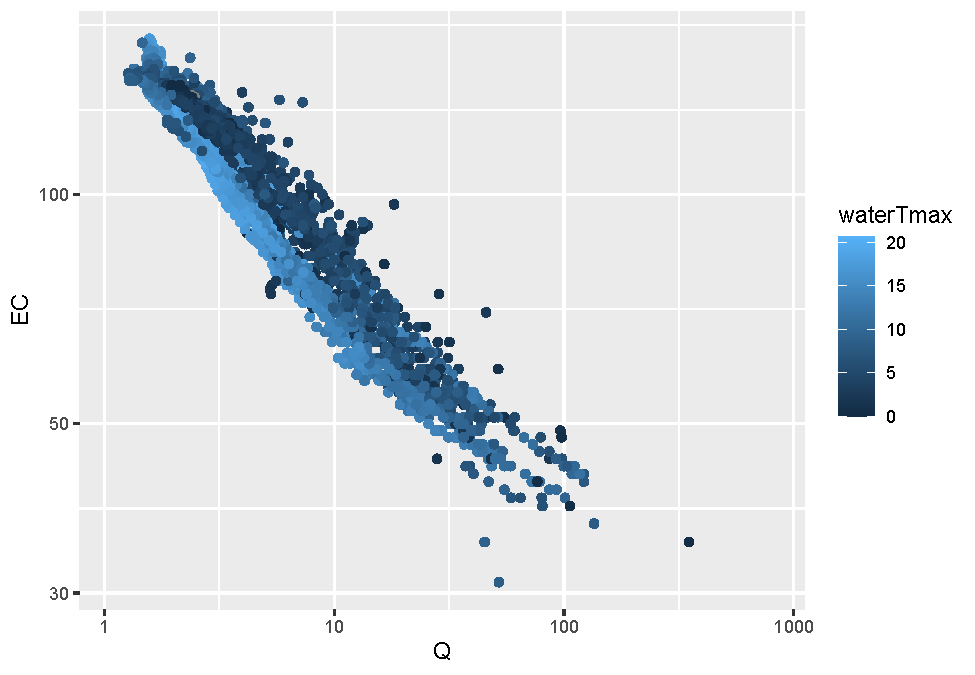
\includegraphics[width=0.75\linewidth]{EnvDataScience_files/figure-latex/visSagehenQECcolorTemp-1} 

}

\caption{Streamflow (Q) and specific electrical conductance (EC) for Sagehen Creek, colored by temperature}\label{fig:visSagehenQECcolorTemp}
\end{figure}

\textbf{River map and profile}

\index{profile}We'll build a \texttt{riverData} dataframe with x and y location values and elevation. We'll need to start by creating empty vectors we'll populate with values in a loop: \texttt{d}, \texttt{longd}, and \texttt{s} are assigned an empty value \texttt{double()}, then slope \texttt{s} (since it only occurs between two points) needs one \texttt{NA} value assigned for the last point \texttt{s{[}length(x{]}} to have the same length as other vectors.

\begin{Shaded}
\begin{Highlighting}[]
\FunctionTok{library}\NormalTok{(tidyverse)}
\NormalTok{x }\OtherTok{\textless{}{-}} \FunctionTok{c}\NormalTok{(}\DecValTok{1000}\NormalTok{, }\DecValTok{1100}\NormalTok{, }\DecValTok{1300}\NormalTok{, }\DecValTok{1500}\NormalTok{, }\DecValTok{1600}\NormalTok{, }\DecValTok{1800}\NormalTok{, }\DecValTok{1900}\NormalTok{)}
\NormalTok{y }\OtherTok{\textless{}{-}} \FunctionTok{c}\NormalTok{(}\DecValTok{500}\NormalTok{, }\DecValTok{780}\NormalTok{, }\DecValTok{820}\NormalTok{, }\DecValTok{950}\NormalTok{, }\DecValTok{1250}\NormalTok{, }\DecValTok{1320}\NormalTok{, }\DecValTok{1500}\NormalTok{)}
\NormalTok{elev }\OtherTok{\textless{}{-}} \FunctionTok{c}\NormalTok{(}\DecValTok{0}\NormalTok{, }\DecValTok{1}\NormalTok{, }\DecValTok{2}\NormalTok{, }\DecValTok{5}\NormalTok{, }\DecValTok{25}\NormalTok{, }\DecValTok{75}\NormalTok{, }\DecValTok{150}\NormalTok{)}
\NormalTok{d }\OtherTok{\textless{}{-}} \FunctionTok{double}\NormalTok{()      }\CommentTok{\# creates an empty numeric vector }
\NormalTok{longd }\OtherTok{\textless{}{-}} \FunctionTok{double}\NormalTok{()  }\CommentTok{\# ("double" means double{-}precision floating point)}
\NormalTok{s }\OtherTok{\textless{}{-}} \FunctionTok{double}\NormalTok{()}
\ControlFlowTok{for}\NormalTok{(i }\ControlFlowTok{in} \DecValTok{1}\SpecialCharTok{:}\FunctionTok{length}\NormalTok{(x))\{}
  \ControlFlowTok{if}\NormalTok{(i}\SpecialCharTok{==}\DecValTok{1}\NormalTok{)\{longd[i] }\OtherTok{\textless{}{-}} \DecValTok{0}\NormalTok{; d[i] }\OtherTok{\textless{}{-}}\DecValTok{0}\NormalTok{\}}
  \ControlFlowTok{else}\NormalTok{\{}
\NormalTok{    d[i] }\OtherTok{\textless{}{-}} \FunctionTok{sqrt}\NormalTok{((x[i]}\SpecialCharTok{{-}}\NormalTok{x[i}\DecValTok{{-}1}\NormalTok{])}\SpecialCharTok{\^{}}\DecValTok{2} \SpecialCharTok{+}\NormalTok{ (y[i]}\SpecialCharTok{{-}}\NormalTok{y[i}\DecValTok{{-}1}\NormalTok{])}\SpecialCharTok{\^{}}\DecValTok{2}\NormalTok{)}
\NormalTok{    longd[i] }\OtherTok{\textless{}{-}}\NormalTok{ longd[i}\DecValTok{{-}1}\NormalTok{] }\SpecialCharTok{+}\NormalTok{ d[i]}
\NormalTok{    s[i}\DecValTok{{-}1}\NormalTok{] }\OtherTok{\textless{}{-}}\NormalTok{ (elev[i]}\SpecialCharTok{{-}}\NormalTok{elev[i}\DecValTok{{-}1}\NormalTok{])}\SpecialCharTok{/}\NormalTok{d[i]\}\}}
\NormalTok{s[}\FunctionTok{length}\NormalTok{(x)] }\OtherTok{\textless{}{-}} \ConstantTok{NA}  \CommentTok{\# make the last slope value NA since we have no data past it, }
                    \CommentTok{\# and so the vector lengths are all the same}
\NormalTok{riverData }\OtherTok{\textless{}{-}} \FunctionTok{bind\_cols}\NormalTok{(}\AttributeTok{x=}\NormalTok{x,}\AttributeTok{y=}\NormalTok{y,}\AttributeTok{elev=}\NormalTok{elev,}\AttributeTok{d=}\NormalTok{d,}\AttributeTok{longd=}\NormalTok{longd,}\AttributeTok{s=}\NormalTok{s)}
\NormalTok{riverData}
\end{Highlighting}
\end{Shaded}

\begin{verbatim}
## # A tibble: 7 x 6
##       x     y  elev     d longd        s
##   <dbl> <dbl> <dbl> <dbl> <dbl>    <dbl>
## 1  1000   500     0    0     0   0.00336
## 2  1100   780     1  297.  297.  0.00490
## 3  1300   820     2  204.  501.  0.0126 
## 4  1500   950     5  239.  740.  0.0632 
## 5  1600  1250    25  316. 1056.  0.236  
## 6  1800  1320    75  212. 1268.  0.364  
## 7  1900  1500   150  206. 1474. NA
\end{verbatim}

For this continuous data, a range of values is detected and a continous color scheme is assigned (Figure \ref{fig:visGreenRed}). The ggplot \texttt{scale\_color\_gradient} function is used to establish end points of a color range that the data is stretched between (Figure \ref{fig:visGreenRedLongProf}). We can use this for many continuous variables, such as slope (Figure \ref{fig:visSlopeLong}). The \texttt{scale\_color\_gradient2} lets you use a \texttt{mid} color. Note that there's a comparable \texttt{scale\_fill\_gradient} and \texttt{scale\_fill\_gradient2} for use when specifying a fill (e.g.~for a polygon) instead of a color (for polygons linked to the border).

\begin{Shaded}
\begin{Highlighting}[]
\FunctionTok{ggplot}\NormalTok{(riverData, }\FunctionTok{aes}\NormalTok{(x,y)) }\SpecialCharTok{+}
  \FunctionTok{geom\_line}\NormalTok{(}\AttributeTok{mapping=}\FunctionTok{aes}\NormalTok{(}\AttributeTok{col=}\NormalTok{s), }\AttributeTok{size=}\FloatTok{1.2}\NormalTok{) }\SpecialCharTok{+} 
  \FunctionTok{geom\_point}\NormalTok{(}\AttributeTok{mapping=}\FunctionTok{aes}\NormalTok{(}\AttributeTok{col=}\NormalTok{s, }\AttributeTok{size=}\NormalTok{elev)) }\SpecialCharTok{+}
  \FunctionTok{coord\_fixed}\NormalTok{(}\AttributeTok{ratio=}\DecValTok{1}\NormalTok{) }\SpecialCharTok{+} \FunctionTok{scale\_color\_gradient}\NormalTok{(}\AttributeTok{low=}\StringTok{"green"}\NormalTok{, }\AttributeTok{high=}\StringTok{"red"}\NormalTok{) }\SpecialCharTok{+}
  \FunctionTok{ggtitle}\NormalTok{(}\StringTok{"Simulated river path, elevations, and slopes"}\NormalTok{)}
\end{Highlighting}
\end{Shaded}

\begin{figure}

{\centering 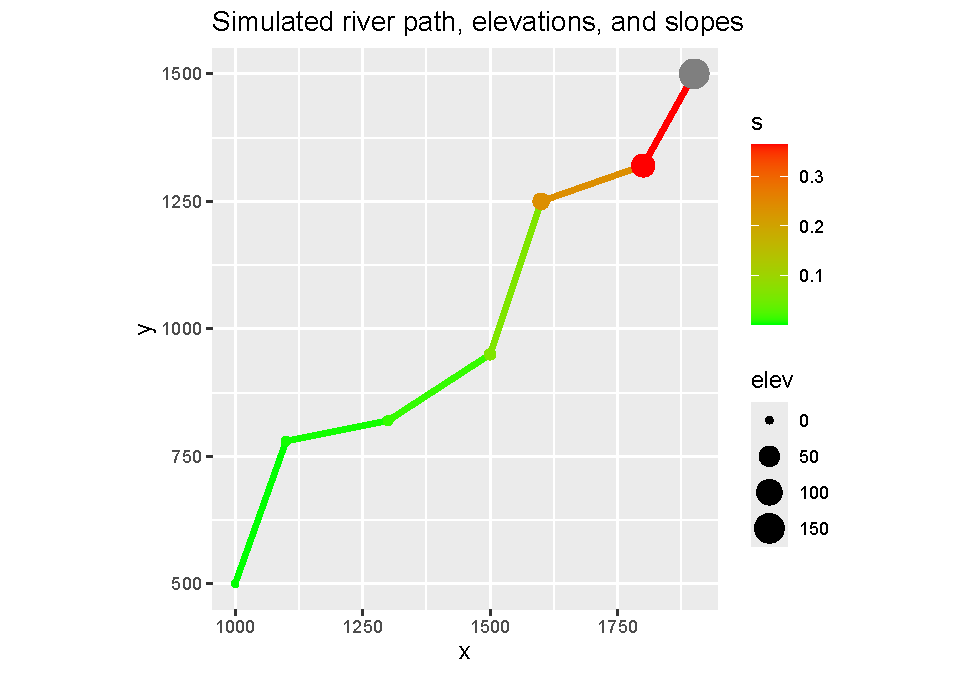
\includegraphics[width=0.75\linewidth]{EnvDataScience_files/figure-latex/visGreenRed-1} 

}

\caption{Channel slope as range from green to red, vertices sized by elevation}\label{fig:visGreenRed}
\end{figure}

\begin{Shaded}
\begin{Highlighting}[]
\FunctionTok{ggplot}\NormalTok{(riverData, }\FunctionTok{aes}\NormalTok{(longd,elev)) }\SpecialCharTok{+} \FunctionTok{geom\_line}\NormalTok{(}\FunctionTok{aes}\NormalTok{(}\AttributeTok{col=}\NormalTok{s), }\AttributeTok{size=}\FloatTok{1.5}\NormalTok{) }\SpecialCharTok{+} \FunctionTok{geom\_point}\NormalTok{()  }\SpecialCharTok{+}
  \FunctionTok{scale\_color\_gradient}\NormalTok{(}\AttributeTok{low=}\StringTok{"green"}\NormalTok{, }\AttributeTok{high=}\StringTok{"red"}\NormalTok{) }\SpecialCharTok{+}
  \FunctionTok{ggtitle}\NormalTok{(}\StringTok{"Longitudinal profile"}\NormalTok{)}
\end{Highlighting}
\end{Shaded}

\begin{figure}

{\centering 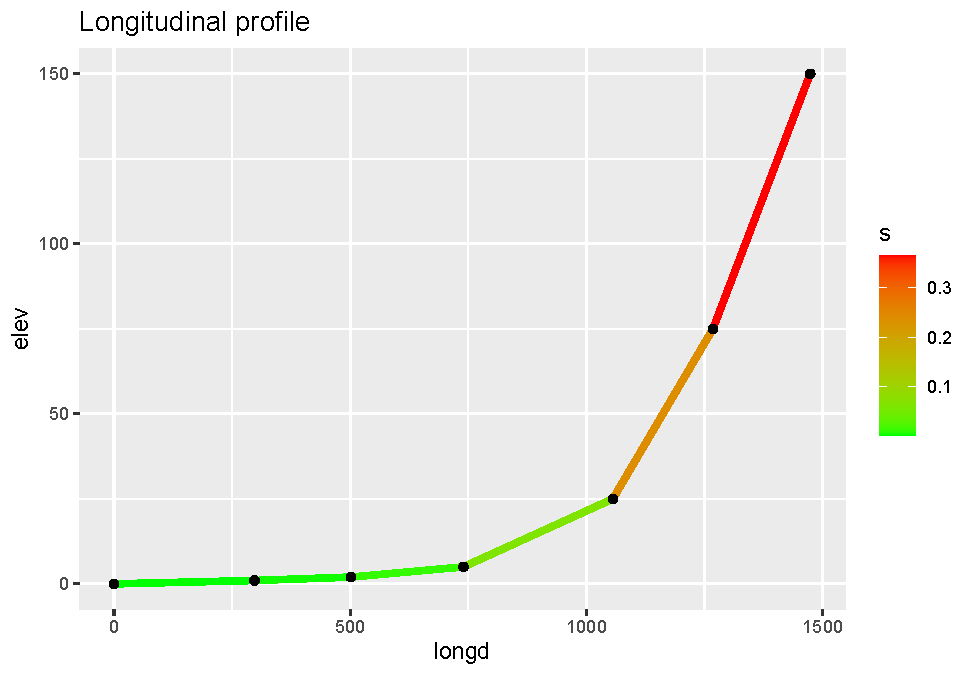
\includegraphics[width=0.75\linewidth]{EnvDataScience_files/figure-latex/visGreenRedLongProf-1} 

}

\caption{Channel slope as range of line colors on a longitudinal profile}\label{fig:visGreenRedLongProf}
\end{figure}

\begin{Shaded}
\begin{Highlighting}[]
\FunctionTok{ggplot}\NormalTok{(riverData, }\FunctionTok{aes}\NormalTok{(longd,s)) }\SpecialCharTok{+} \FunctionTok{geom\_point}\NormalTok{(}\FunctionTok{aes}\NormalTok{(}\AttributeTok{col=}\NormalTok{s), }\AttributeTok{size=}\DecValTok{3}\NormalTok{) }\SpecialCharTok{+}
  \FunctionTok{scale\_color\_gradient}\NormalTok{(}\AttributeTok{low=}\StringTok{"green"}\NormalTok{, }\AttributeTok{high=}\StringTok{"red"}\NormalTok{) }\SpecialCharTok{+}
  \FunctionTok{ggtitle}\NormalTok{(}\StringTok{"Slope by longitudinal distance upstream"}\NormalTok{)}
\end{Highlighting}
\end{Shaded}

\begin{figure}

{\centering 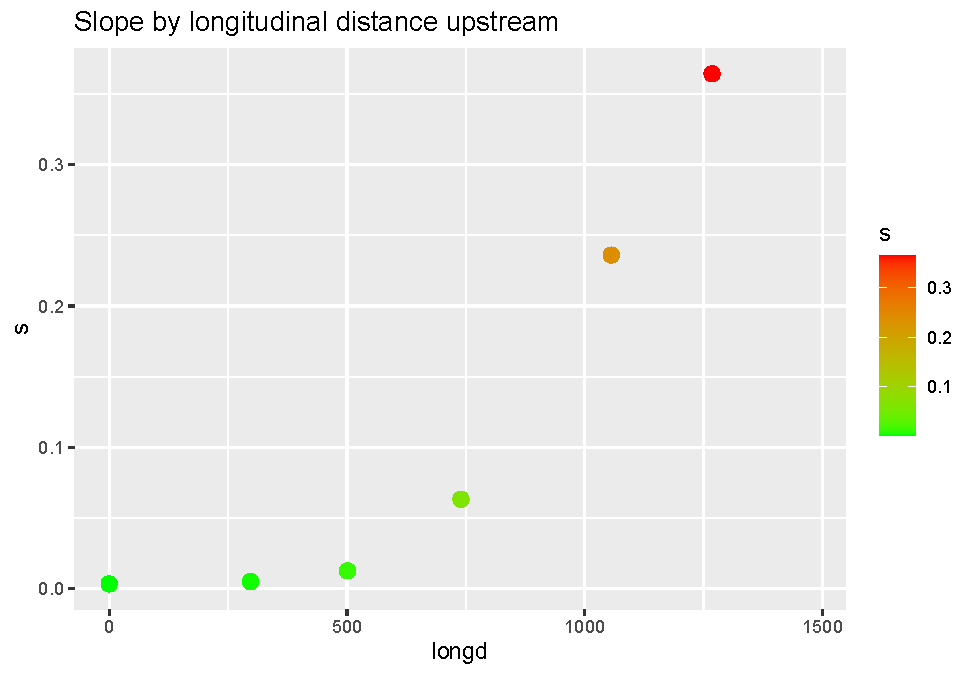
\includegraphics[width=0.75\linewidth]{EnvDataScience_files/figure-latex/visSlopeLong-1} 

}

\caption{Channel slope by longitudinal distance as scatter points colored by slope}\label{fig:visSlopeLong}
\end{figure}

\subsection{Trend line}\label{trend-line}

\index{trend line}When we get to statistical models, the first one we'll look at is a simple linear model. It's often useful to display this as a \emph{trend line}, and this can be done with ggplot2's \texttt{geom\_smooth()} function, specifying the linear model ``lm'' method. By default, the graph displays the standard error as a gray pattern (Figure \ref{fig:visTrendLine}).

\begin{Shaded}
\begin{Highlighting}[]
\NormalTok{sierraFeb }\SpecialCharTok{\%\textgreater{}\%}
  \FunctionTok{ggplot}\NormalTok{(}\FunctionTok{aes}\NormalTok{(TEMPERATURE,ELEVATION)) }\SpecialCharTok{+}
  \FunctionTok{geom\_point}\NormalTok{(}\AttributeTok{color=}\StringTok{"blue"}\NormalTok{) }\SpecialCharTok{+}
  \FunctionTok{geom\_smooth}\NormalTok{(}\AttributeTok{color=}\StringTok{"red"}\NormalTok{, }\AttributeTok{method=}\StringTok{"lm"}\NormalTok{)}
\end{Highlighting}
\end{Shaded}

\begin{figure}

{\centering 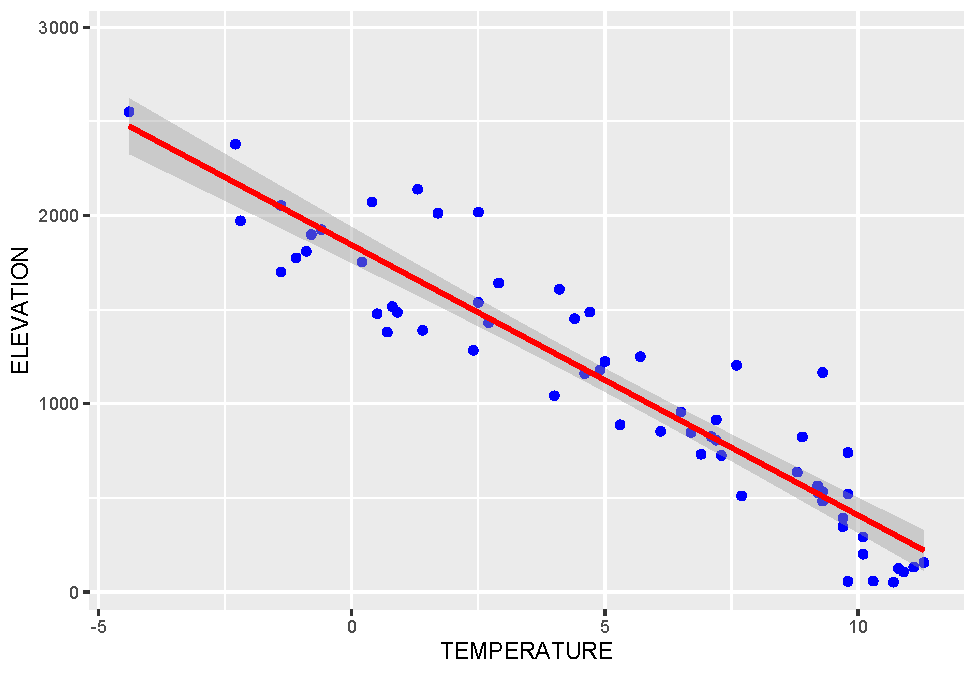
\includegraphics[width=0.75\linewidth]{EnvDataScience_files/figure-latex/visTrendLine-1} 

}

\caption{Trend line with a linear model}\label{fig:visTrendLine}
\end{figure}

\section{General Symbology}\label{general-symbology}

There's a lot to learn about symbology in graphs. We've included the basics, but readers are encouraged to also explore further. A useful vignette accessed by \texttt{vignette("ggplot2-specs")} lets you see aesthetic specifications for symbols, including:

\begin{itemize}
\item
  Color and fill
\item
  Lines

  \begin{itemize}
  \tightlist
  \item
    line type, size, ends
  \end{itemize}
\item
  Polygon

  \begin{itemize}
  \tightlist
  \item
    border color, linetype, size
  \item
    fill
  \end{itemize}
\item
  Points

  \begin{itemize}
  \tightlist
  \item
    shape
  \item
    size
  \item
    color and fill
  \item
    stroke
  \end{itemize}
\item
  Text

  \begin{itemize}
  \tightlist
  \item
    font face and size
  \item
    justification
  \end{itemize}
\end{itemize}

\subsection{Categorical symbology}\label{categorical-symbology}

\index{categorical symbology}One example of a ``big data'' resource is EPA's Toxic Release Inventory that tracks releases from a wide array of sources, from oil refineries on down. One way of dealing with big data in terms of exploring meaning is to use symbology to try to make sense of it (Figure \ref{fig:visTRIcategorical}).

\begin{Shaded}
\begin{Highlighting}[]
\FunctionTok{library}\NormalTok{(igisci)}
\NormalTok{TRI }\OtherTok{\textless{}{-}} \FunctionTok{read\_csv}\NormalTok{(}\FunctionTok{ex}\NormalTok{(}\StringTok{"TRI/TRI\_2017\_CA.csv"}\NormalTok{)) }\SpecialCharTok{\%\textgreater{}\%}
  \FunctionTok{filter}\NormalTok{(}\StringTok{\textasciigrave{}}\AttributeTok{5.1\_FUGITIVE\_AIR}\StringTok{\textasciigrave{}} \SpecialCharTok{\textgreater{}} \DecValTok{100} \SpecialCharTok{\&} 
         \StringTok{\textasciigrave{}}\AttributeTok{5.2\_STACK\_AIR}\StringTok{\textasciigrave{}} \SpecialCharTok{\textgreater{}} \DecValTok{100} \SpecialCharTok{\&} 
         \StringTok{\textasciigrave{}}\AttributeTok{INDUSTRY\_SECTOR}\StringTok{\textasciigrave{}} \SpecialCharTok{!=} \StringTok{"Other"}\NormalTok{)}
\FunctionTok{ggplot}\NormalTok{(}\AttributeTok{data =}\NormalTok{ TRI, }\FunctionTok{aes}\NormalTok{(}\FunctionTok{log}\NormalTok{(}\StringTok{\textasciigrave{}}\AttributeTok{5.2\_STACK\_AIR}\StringTok{\textasciigrave{}}\NormalTok{), }\FunctionTok{log}\NormalTok{(}\StringTok{\textasciigrave{}}\AttributeTok{5.1\_FUGITIVE\_AIR}\StringTok{\textasciigrave{}}\NormalTok{), }
                       \AttributeTok{color =}\NormalTok{ INDUSTRY\_SECTOR)) }\SpecialCharTok{+}
       \FunctionTok{geom\_point}\NormalTok{()}
\end{Highlighting}
\end{Shaded}

\begin{figure}

{\centering 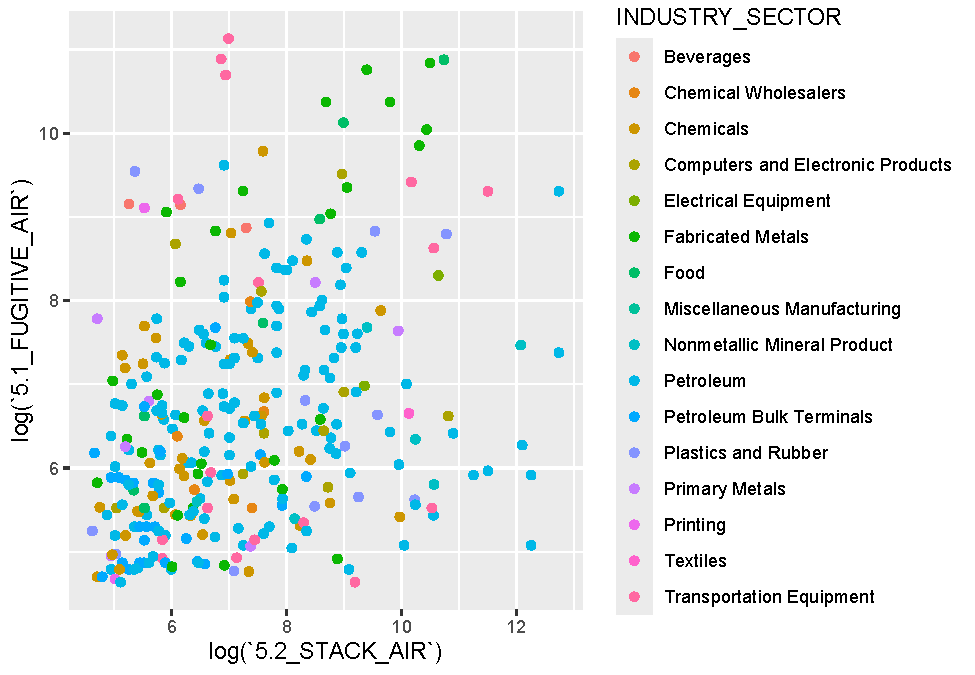
\includegraphics[width=0.75\linewidth]{EnvDataScience_files/figure-latex/visTRIcategorical-1} 

}

\caption{EPA TRI, categorical symbology for industry sector}\label{fig:visTRIcategorical}
\end{figure}

\subsection{Log scales instead of transform}\label{log-scales-instead-of-transform}

\index{log scales}In the above graph, we used the log() function in aes to use natural logarithms instead of the actual value. That's a simple way to do this. But what if we want to display the original data, just using a logarithmic grid? This might communicate better since readers would see the actual values (Figure \ref{fig:visLogScalesTRI}).

\begin{Shaded}
\begin{Highlighting}[]
\FunctionTok{ggplot}\NormalTok{(}\AttributeTok{data=}\NormalTok{TRI, }\FunctionTok{aes}\NormalTok{(}\StringTok{\textasciigrave{}}\AttributeTok{5.2\_STACK\_AIR}\StringTok{\textasciigrave{}}\NormalTok{,}\StringTok{\textasciigrave{}}\AttributeTok{5.1\_FUGITIVE\_AIR}\StringTok{\textasciigrave{}}\NormalTok{,}\AttributeTok{color=}\NormalTok{INDUSTRY\_SECTOR)) }\SpecialCharTok{+}
       \FunctionTok{geom\_point}\NormalTok{() }\SpecialCharTok{+} \FunctionTok{scale\_x\_log10}\NormalTok{() }\SpecialCharTok{+} \FunctionTok{scale\_y\_log10}\NormalTok{()}
\end{Highlighting}
\end{Shaded}

\begin{figure}

{\centering 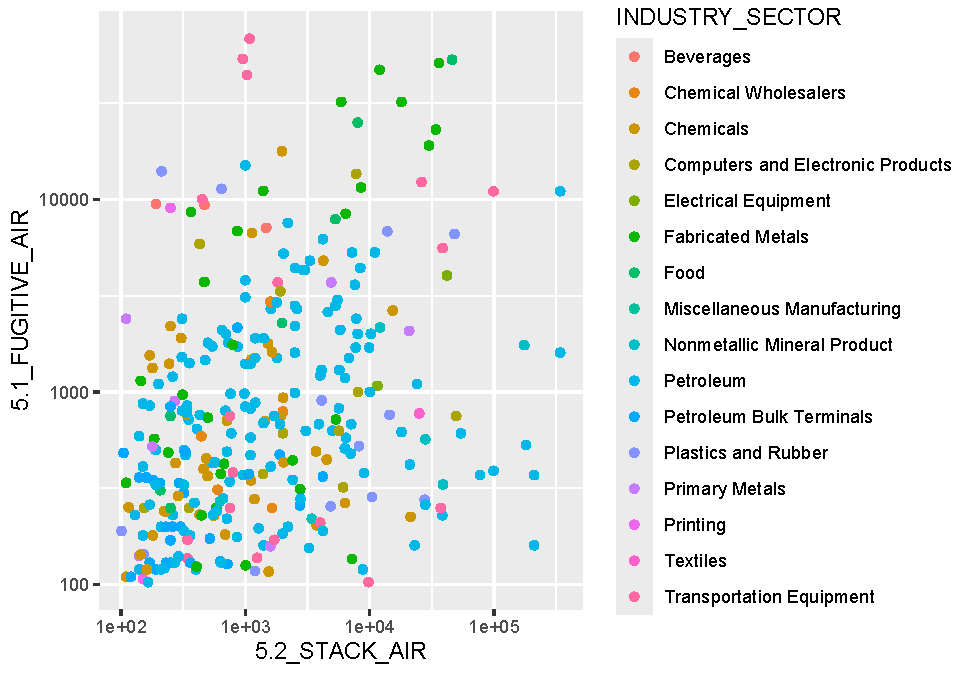
\includegraphics[width=0.75\linewidth]{EnvDataScience_files/figure-latex/visLogScalesTRI-1} 

}

\caption{Using log scales instead of transforming}\label{fig:visLogScalesTRI}
\end{figure}

\section{Graphs from Grouped Data}\label{graphs-from-grouped-data}

\index{grouped data}Earlier in this chapter, we used a pivot table to create a data frame \texttt{XSptsPheno}, which has NDVI values for phenology factors. {[}You may need to run that again if you haven't run it yet this session.{]} We can create graphs showing the relationship of NDVI and elevation grouped by phenology (Figure \ref{fig:visNDVIpheno}).

\begin{Shaded}
\begin{Highlighting}[]
\NormalTok{XSptsPheno }\SpecialCharTok{\%\textgreater{}\%}
  \FunctionTok{ggplot}\NormalTok{() }\SpecialCharTok{+}
  \FunctionTok{geom\_point}\NormalTok{(}\FunctionTok{aes}\NormalTok{(elevation, NDVI, }\AttributeTok{shape=}\NormalTok{vegetation, }
                 \AttributeTok{color =}\NormalTok{ phenology), }\AttributeTok{size =} \DecValTok{3}\NormalTok{) }\SpecialCharTok{+}
  \FunctionTok{geom\_smooth}\NormalTok{(}\FunctionTok{aes}\NormalTok{(elevation, NDVI, }
                 \AttributeTok{color =}\NormalTok{ phenology), }\AttributeTok{method=}\StringTok{"lm"}\NormalTok{) }
\end{Highlighting}
\end{Shaded}

\begin{figure}

{\centering 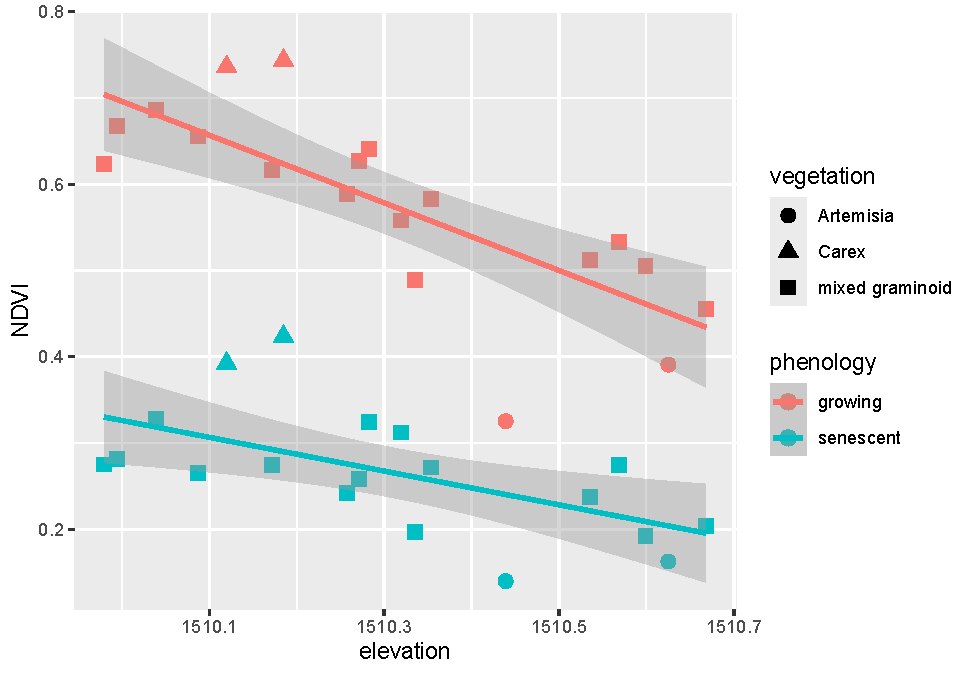
\includegraphics[width=0.75\linewidth]{EnvDataScience_files/figure-latex/visNDVIpheno-1} 

}

\caption{NDVI symbolized by vegetation in two seasons}\label{fig:visNDVIpheno}
\end{figure}

And similarly, we can create graphs of rainfall vs.~runoff for eucs and oaks from the \texttt{tidy\_eucoak} dataframe from the Thompson et al. (\citeproc{ref-eucoak}{2016}) study {[}and you may need to run that again to prep the data{]} (Figure \ref{fig:visEucOakRainfallRunoff}).

\begin{Shaded}
\begin{Highlighting}[]
\FunctionTok{ggplot}\NormalTok{(}\AttributeTok{data =}\NormalTok{ tidy\_eucoak) }\SpecialCharTok{+}
  \FunctionTok{geom\_point}\NormalTok{(}\AttributeTok{mapping =} \FunctionTok{aes}\NormalTok{(}\AttributeTok{x =}\NormalTok{ rain\_mm, }\AttributeTok{y =}\NormalTok{ runoff\_L, }\AttributeTok{color =}\NormalTok{ tree)) }\SpecialCharTok{+}
  \FunctionTok{geom\_smooth}\NormalTok{(}\AttributeTok{mapping =} \FunctionTok{aes}\NormalTok{(}\AttributeTok{x =}\NormalTok{ rain\_mm, }\AttributeTok{y=}\NormalTok{ runoff\_L, }\AttributeTok{color =}\NormalTok{ tree), }
              \AttributeTok{method =} \StringTok{"lm"}\NormalTok{) }\SpecialCharTok{+}
  \FunctionTok{scale\_color\_manual}\NormalTok{(}\AttributeTok{values =} \FunctionTok{c}\NormalTok{(}\StringTok{"seagreen4"}\NormalTok{, }\StringTok{"orange3"}\NormalTok{))}
\end{Highlighting}
\end{Shaded}

\begin{figure}

{\centering 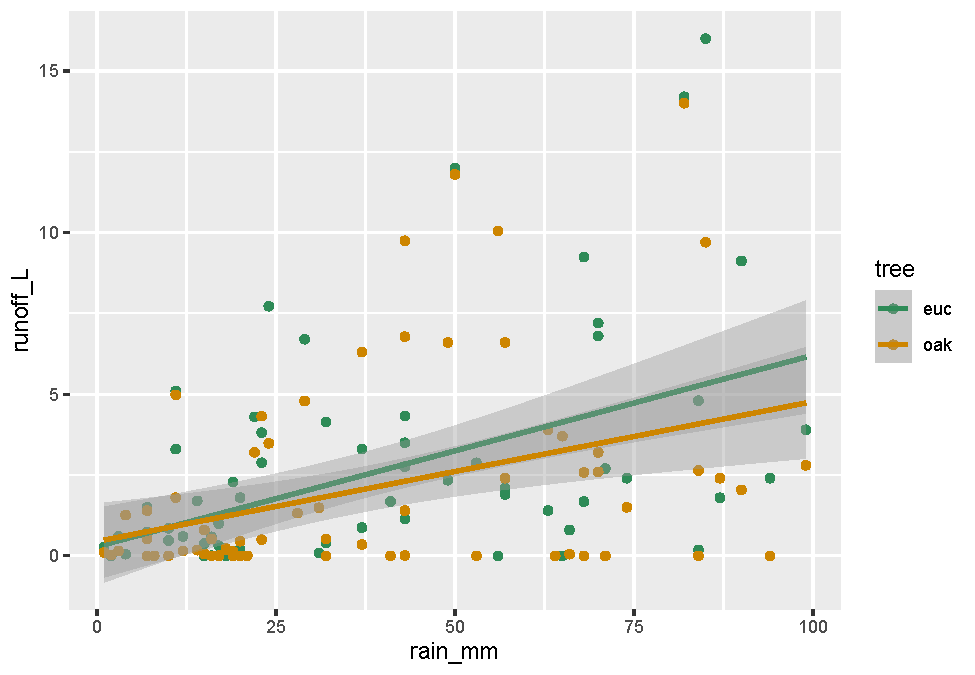
\includegraphics[width=0.75\linewidth]{EnvDataScience_files/figure-latex/visEucOakRainfallRunoff-1} 

}

\caption{Eucalyptus and oak: rainfall and runoff}\label{fig:visEucOakRainfallRunoff}
\end{figure}

\subsection{Faceted graphs}\label{faceted-graphs}

\index{faceted graphs}A theme we've already seen in this chapter is communicating more by comparing data on the same graph. We've been using symbology for that, but another approach is to create parallel groups of graphs called ``faceted graphs'' (Figure \ref{fig:visFacetedGraph}).

\begin{Shaded}
\begin{Highlighting}[]
\FunctionTok{ggplot}\NormalTok{(}\AttributeTok{data =}\NormalTok{ tidy\_eucoak) }\SpecialCharTok{+}
  \FunctionTok{geom\_point}\NormalTok{(}\FunctionTok{aes}\NormalTok{(}\AttributeTok{x=}\NormalTok{rain\_mm,}\AttributeTok{y=}\NormalTok{runoff\_L)) }\SpecialCharTok{+}
  \FunctionTok{geom\_smooth}\NormalTok{(}\FunctionTok{aes}\NormalTok{(}\AttributeTok{x=}\NormalTok{rain\_mm,}\AttributeTok{y=}\NormalTok{runoff\_L), }\AttributeTok{method=}\StringTok{"lm"}\NormalTok{) }\SpecialCharTok{+}
  \FunctionTok{facet\_grid}\NormalTok{(tree }\SpecialCharTok{\textasciitilde{}}\NormalTok{ .)}
\end{Highlighting}
\end{Shaded}

\begin{figure}

{\centering 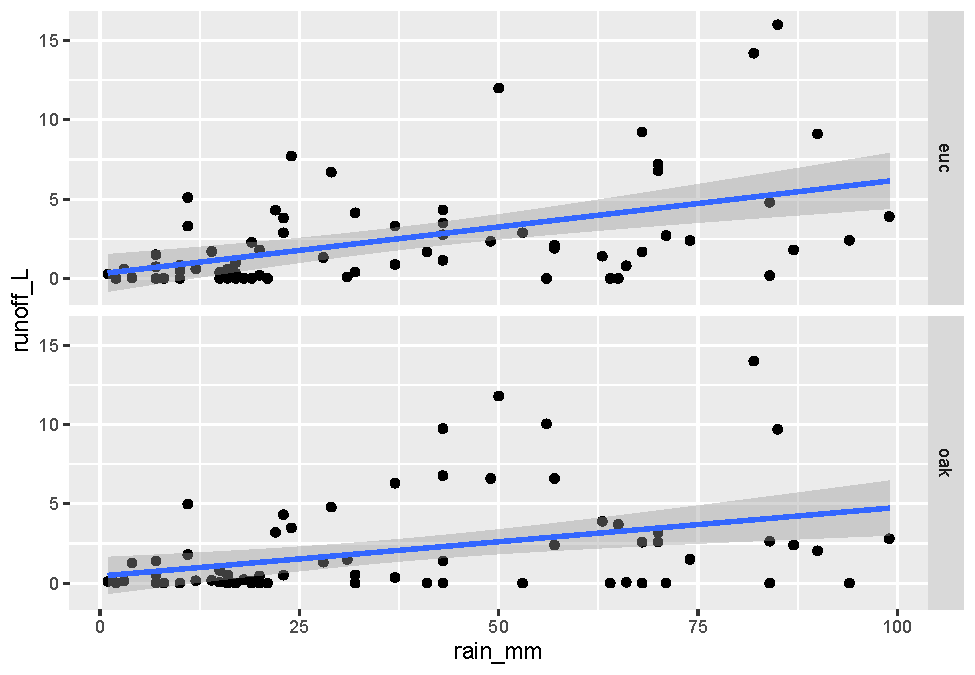
\includegraphics[width=0.75\linewidth]{EnvDataScience_files/figure-latex/visFacetedGraph-1} 

}

\caption{Faceted graph alternative to color grouping (note that the y scale is the same for each)}\label{fig:visFacetedGraph}
\end{figure}

Note that the y scale is the same for each, which is normally what you want since each graph is representing the same variable. If you were displaying different variables, however, you'd want to use the \texttt{scales\ =\ "free\_y"} setting.

\begin{quote}
Again, we'll learn about pivot tables in the next chapter to set up our data.
\end{quote}

\section{Titles, Subtitles, Axis Labels, and Legend Position}\label{titles-subtitles-axis-labels-and-legend-position}

\index{titles}All graphs need titles, and ggplot2 uses its \texttt{labs()} function for this (Figure \ref{fig:visTitles}) as well as for subtitles and axis label improvements.

\begin{Shaded}
\begin{Highlighting}[]
\FunctionTok{ggplot}\NormalTok{(}\AttributeTok{data =}\NormalTok{ tidy\_eucoak) }\SpecialCharTok{+}
  \FunctionTok{geom\_point}\NormalTok{(}\FunctionTok{aes}\NormalTok{(}\AttributeTok{x=}\NormalTok{rain\_mm,}\AttributeTok{y=}\NormalTok{runoff\_L, }\AttributeTok{color=}\NormalTok{tree)) }\SpecialCharTok{+}
  \FunctionTok{geom\_smooth}\NormalTok{(}\FunctionTok{aes}\NormalTok{(}\AttributeTok{x=}\NormalTok{rain\_mm,}\AttributeTok{y=}\NormalTok{runoff\_L, }\AttributeTok{color=}\NormalTok{tree), }\AttributeTok{method=}\StringTok{"lm"}\NormalTok{) }\SpecialCharTok{+}
  \FunctionTok{scale\_color\_manual}\NormalTok{(}\AttributeTok{values=}\FunctionTok{c}\NormalTok{(}\StringTok{"seagreen4"}\NormalTok{,}\StringTok{"orange3"}\NormalTok{)) }\SpecialCharTok{+}
  \FunctionTok{labs}\NormalTok{(}\AttributeTok{title=}\StringTok{"rainfall \textasciitilde{} runoff"}\NormalTok{, }
       \AttributeTok{subtitle=}\StringTok{"eucalyptus \& oak sites, 2016"}\NormalTok{,}
       \AttributeTok{x=}\StringTok{"Rain (mm)"}\NormalTok{,}
       \AttributeTok{y=}\StringTok{"runoff (L)"}\NormalTok{) }\SpecialCharTok{+}
  \FunctionTok{theme}\NormalTok{(}\AttributeTok{legend.position =} \FunctionTok{c}\NormalTok{(}\FloatTok{0.1}\NormalTok{,}\FloatTok{0.8}\NormalTok{))}
\end{Highlighting}
\end{Shaded}

\begin{figure}

{\centering 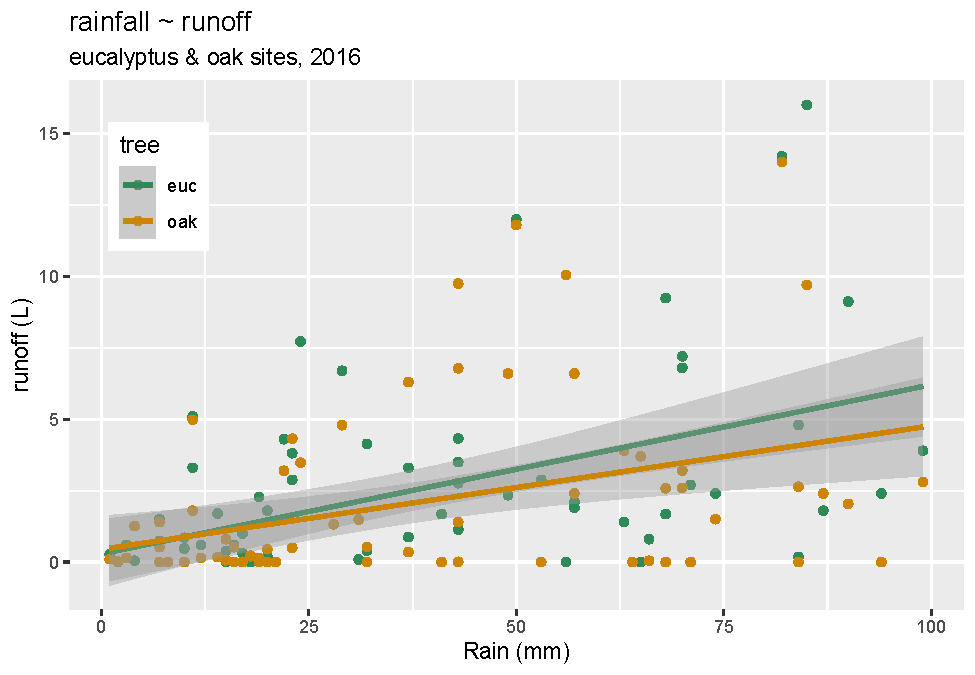
\includegraphics[width=0.75\linewidth]{EnvDataScience_files/figure-latex/visTitles-1} 

}

\caption{Titles added}\label{fig:visTitles}
\end{figure}

\begin{quote}
Note that we also used the \texttt{theme(legend.position)} setting to set the position of the legend as x and y values as a proportion of the graph dimensions. See \texttt{?theme} to see the wide variety of changes that can be made to modify your plot from the default settings.
\end{quote}

\section{Pairs Plot}\label{pairs-plot}

\index{pairs plot}Pairs plots are an excellent exploratory tool to see which variables are correlated. Since only continuous data is useful for this, and since pairs plots can quickly get overly complex, it's good to use \texttt{dplyr::select} to select the continuous variables, or maybe use a helper function like \texttt{is.numeric} with \texttt{dplyr::select\_if} (Figure \ref{fig:visPairsPlot}).

\begin{Shaded}
\begin{Highlighting}[]
\NormalTok{sierraFeb }\SpecialCharTok{\%\textgreater{}\%}
\NormalTok{     dplyr}\SpecialCharTok{::}\FunctionTok{select}\NormalTok{(ELEVATION}\SpecialCharTok{:}\NormalTok{TEMPERATURE) }\SpecialCharTok{\%\textgreater{}\%}
     \FunctionTok{pairs}\NormalTok{()}
\end{Highlighting}
\end{Shaded}

\begin{figure}

{\centering 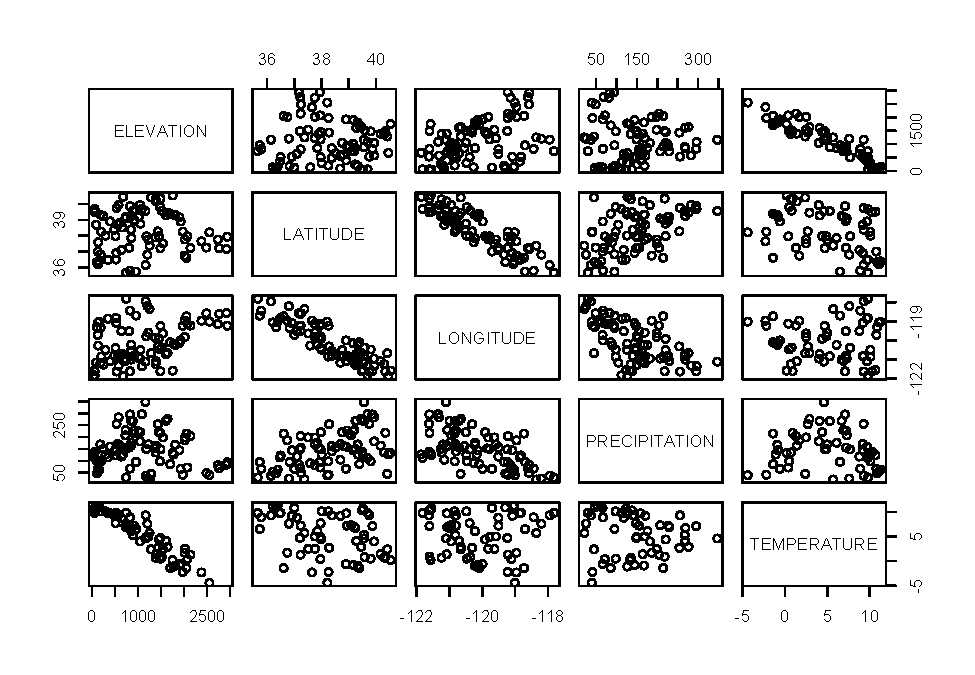
\includegraphics[width=0.75\linewidth]{EnvDataScience_files/figure-latex/visPairsPlot-1} 

}

\caption{Pairs plot for Sierra Nevada stations variables}\label{fig:visPairsPlot}
\end{figure}

The GGally package has a very nice-looking pairs plot that takes it even further. In addition to scatterplots, it has boxplots, histograms, density plots, and correlations, all stratified and colored by species. The code for this figure is mostly borrowed from Horst et al. (\citeproc{ref-palmer}{2020}) (Figure \ref{fig:visGGallyPenguins}).

\begin{Shaded}
\begin{Highlighting}[]
\FunctionTok{library}\NormalTok{(palmerpenguins)}
\NormalTok{penguins }\SpecialCharTok{\%\textgreater{}\%}
\NormalTok{  dplyr}\SpecialCharTok{::}\FunctionTok{select}\NormalTok{(species, body\_mass\_g, }\FunctionTok{ends\_with}\NormalTok{(}\StringTok{"\_mm"}\NormalTok{)) }\SpecialCharTok{\%\textgreater{}\%}
\NormalTok{  GGally}\SpecialCharTok{::}\FunctionTok{ggpairs}\NormalTok{(}\FunctionTok{aes}\NormalTok{(}\AttributeTok{color =}\NormalTok{ species, }\AttributeTok{alpha =} \FloatTok{0.8}\NormalTok{)) }\SpecialCharTok{+}
  \FunctionTok{scale\_colour\_manual}\NormalTok{(}\AttributeTok{values =} \FunctionTok{c}\NormalTok{(}\StringTok{"darkorange"}\NormalTok{,}\StringTok{"purple"}\NormalTok{,}\StringTok{"cyan4"}\NormalTok{)) }\SpecialCharTok{+}
  \FunctionTok{scale\_fill\_manual}\NormalTok{(}\AttributeTok{values =} \FunctionTok{c}\NormalTok{(}\StringTok{"darkorange"}\NormalTok{,}\StringTok{"purple"}\NormalTok{,}\StringTok{"cyan4"}\NormalTok{))}
\end{Highlighting}
\end{Shaded}

\begin{figure}

{\centering 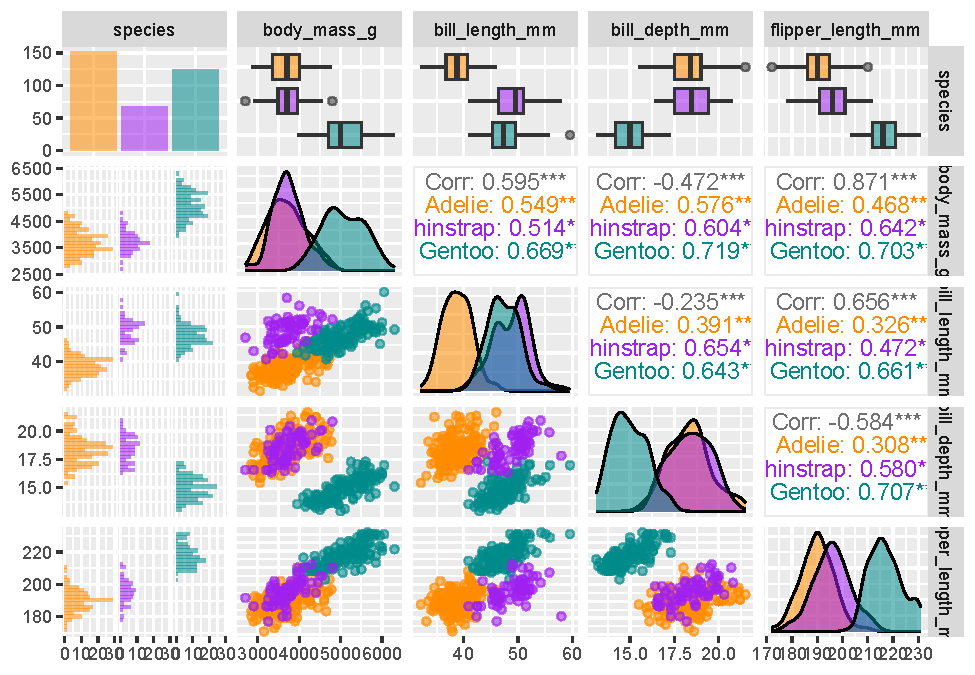
\includegraphics[width=0.75\linewidth]{EnvDataScience_files/figure-latex/visGGallyPenguins-1} 

}

\caption{Enhanced GGally pairs plot for palmerpenguin data}\label{fig:visGGallyPenguins}
\end{figure}

\pagebreak

\section{Exercises: Visualization}\label{exercises-visualization}

\begin{exercise}

Using the methods in section 4.3, create a similar graph of the species data set we looked at in section

\begin{center}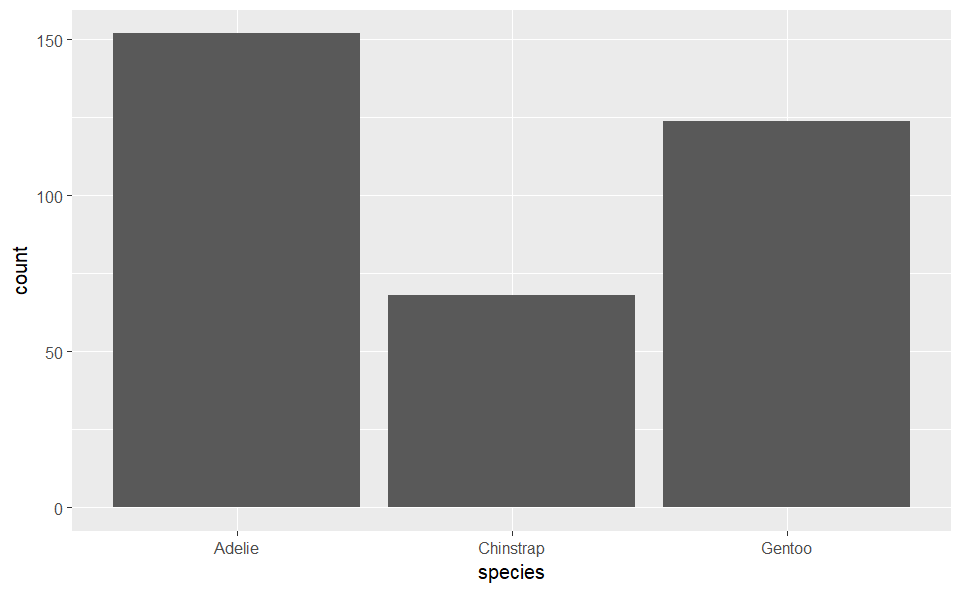
\includegraphics[width=0.75\linewidth]{img/vis.ex1} \end{center}

\end{exercise}

\begin{exercise}

Using similar methods as we just used, create the graph shown below. First, explore the built-in vectors \texttt{state.abb} and \texttt{state.region} to learn about how they are structured. Then, using methods described in 2.6.4.2, create a single data frame from those inputs. Once you've explored that result, create the graph.

\begin{center}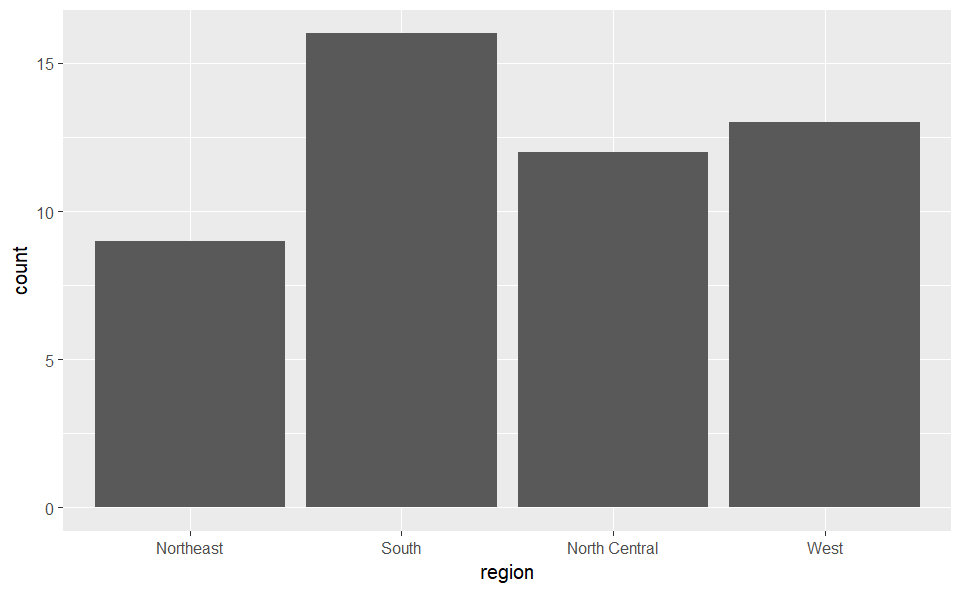
\includegraphics[width=0.75\linewidth]{img/vis.ex2} \end{center}

\end{exercise}

\begin{exercise}

Create the graph below using methods described in 4.3.3.1, using the built-in data set you can see labeled on the x axis. You'll want to start by exploring the data set and learning about it by accessing the simple ``?\_\_\_'' help system; then convert it into a suitable data structure.

\begin{center}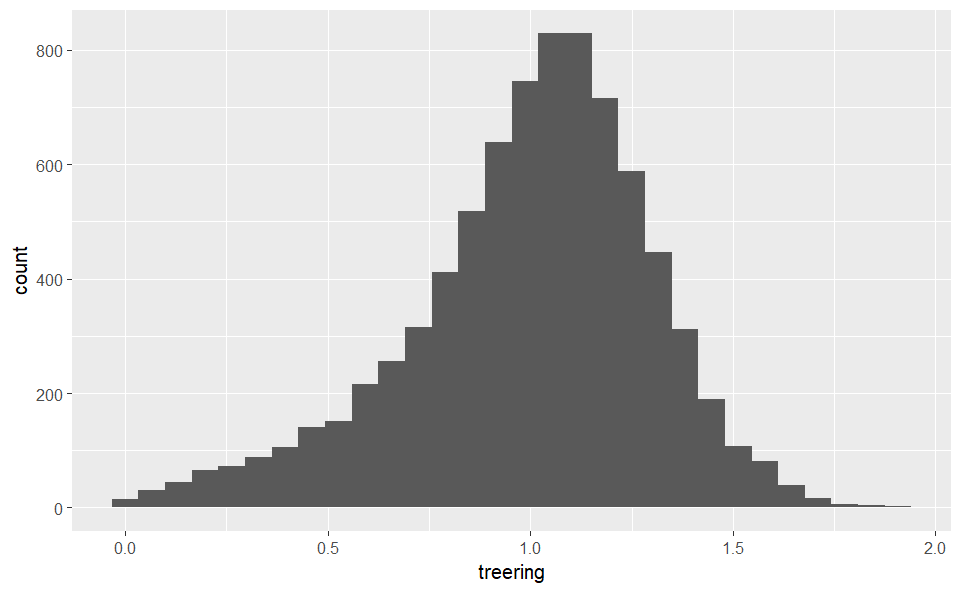
\includegraphics[width=0.75\linewidth]{img/vis.ex3} \end{center}

\end{exercise}

\begin{exercise}

Have a look at the \texttt{st} tibble created in 3.2.1.1, and then use it to create the graph shown here, using methods similar to 4.3.2. What is the approximate modal value?

\begin{center}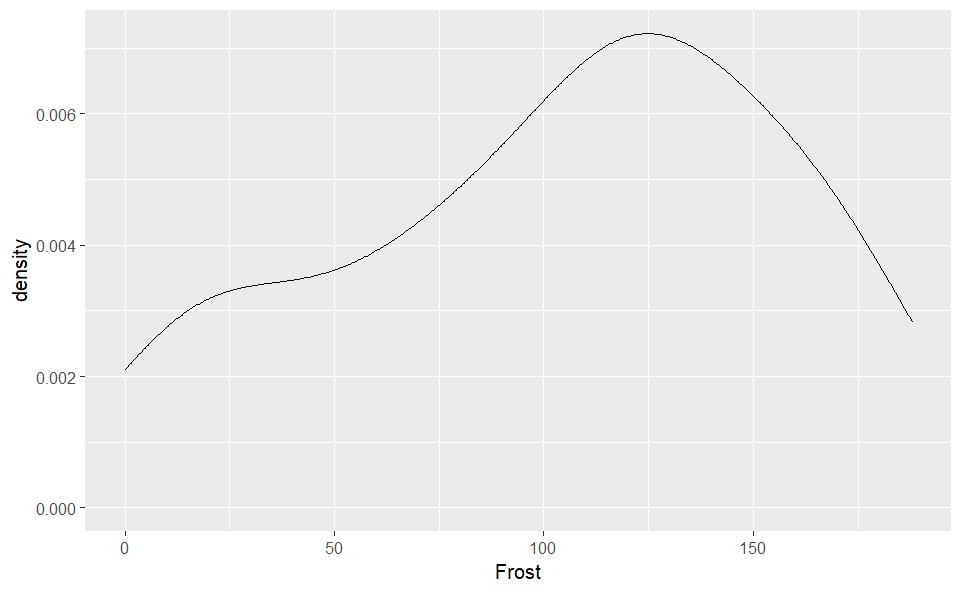
\includegraphics[width=0.75\linewidth]{img/vis.ex4} \end{center}

\end{exercise}

\begin{exercise}

From the same data, create the following graphs using methods learned in this chapter. What can you learn about the regions from the median values shown?

\begin{center}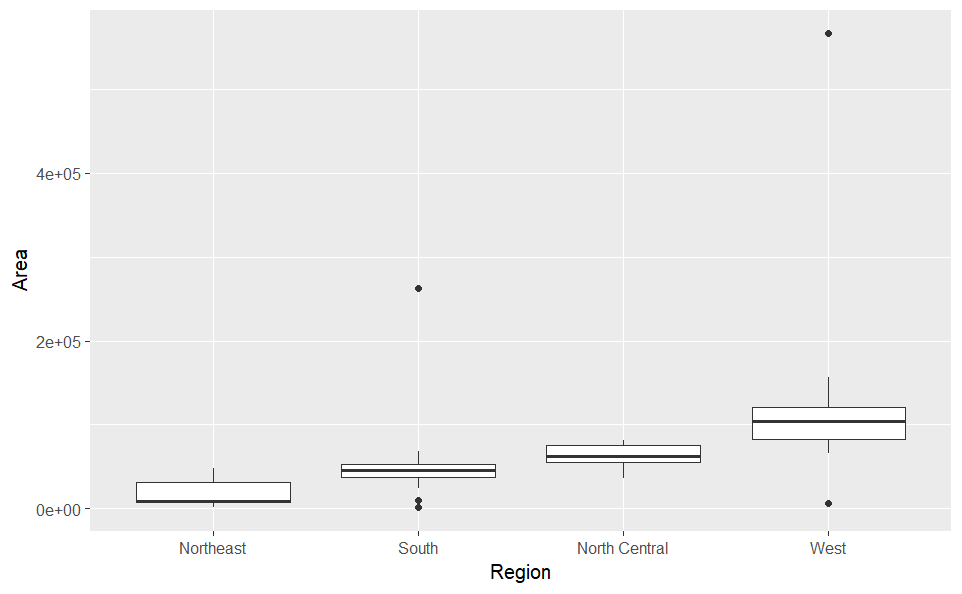
\includegraphics[width=0.75\linewidth]{img/vis.ex5a} \end{center}

\begin{center}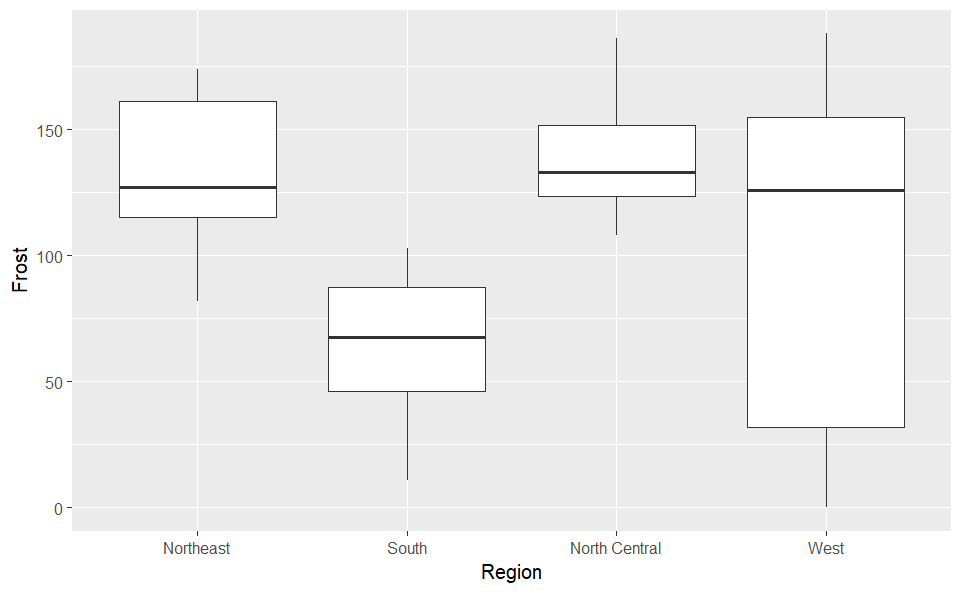
\includegraphics[width=0.75\linewidth]{img/vis.ex5b} \end{center}

\end{exercise}

\begin{exercise}

From the same data, create the scatter plot shown below.

\begin{center}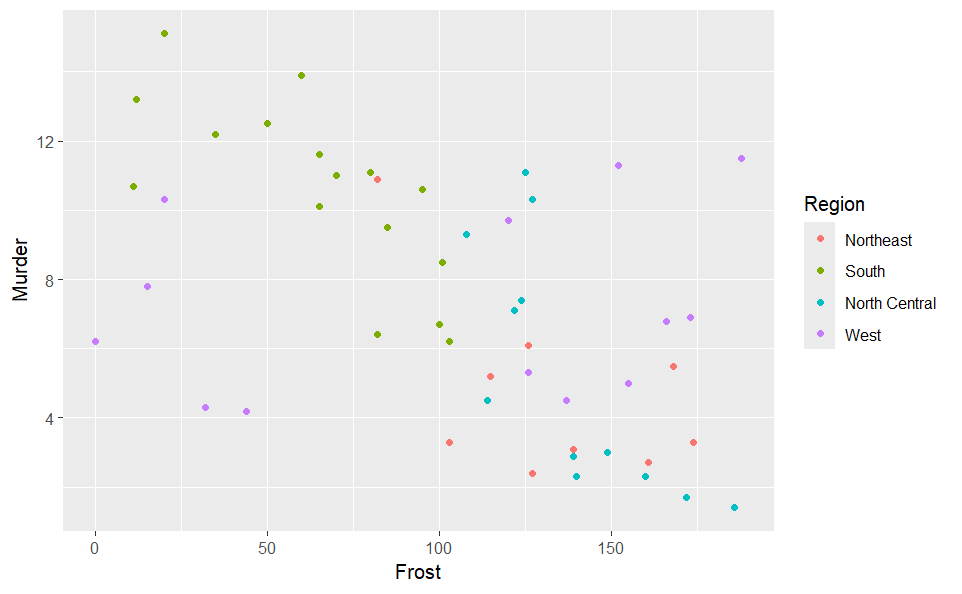
\includegraphics[width=0.75\linewidth]{img/vis.ex6} \end{center}

\end{exercise}

\begin{exercise}

Copying the above code to a new code chunk, add a trend line using methods in 3.4.4 to produce the graph shown here. What can you say about what this graph is showing you?

\begin{center}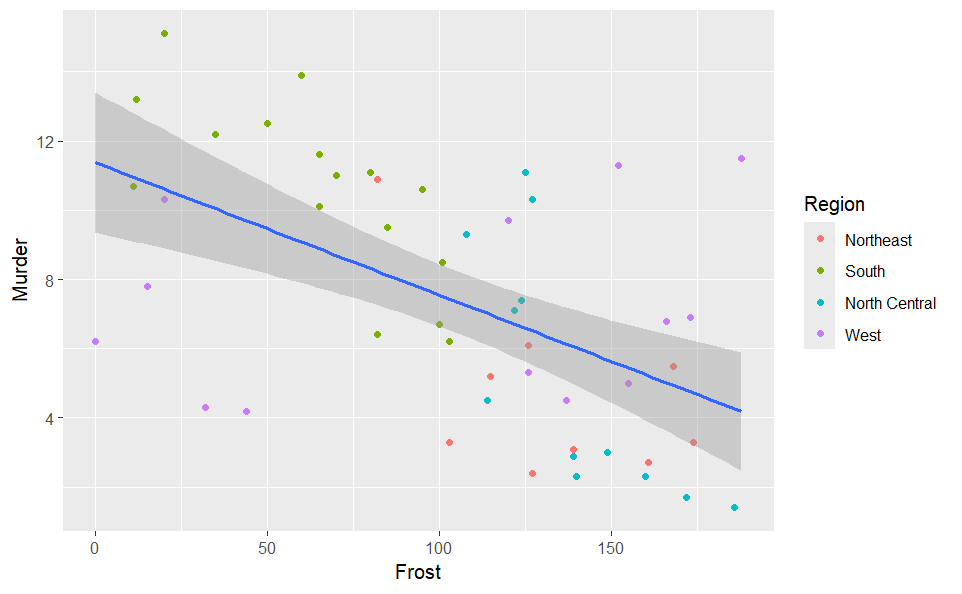
\includegraphics[width=0.75\linewidth]{img/vis.ex7} \end{center}

\end{exercise}

\begin{exercise}

Again, copying the code to a new code chunk, add an appropriate title, as shown here.

\begin{center}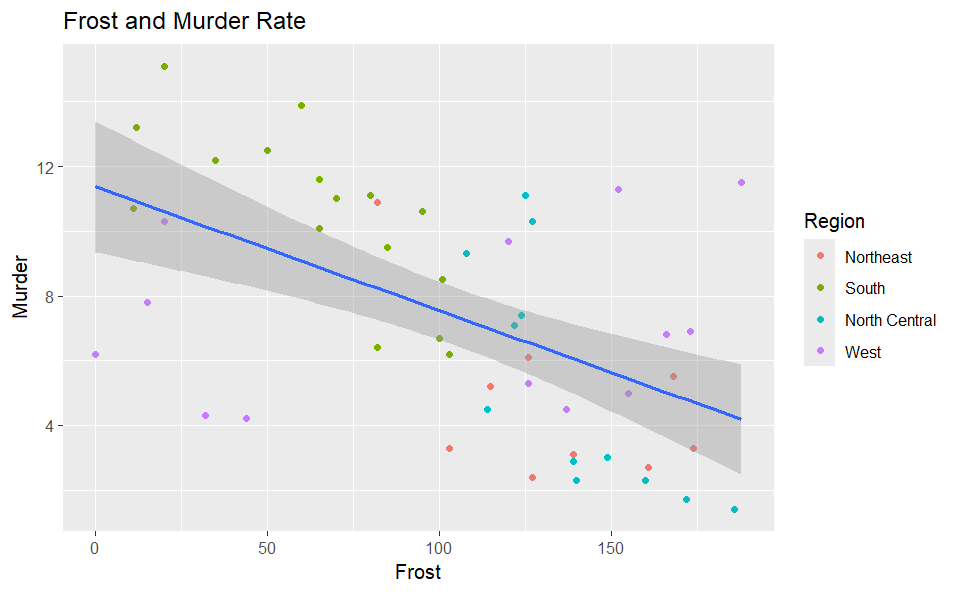
\includegraphics[width=0.75\linewidth]{img/vis.ex8} \end{center}

\end{exercise}

\begin{exercise}

Again copying to a new code chunk, change your plot to place labels with symbology shown here. Any observations about outliers?

\begin{center}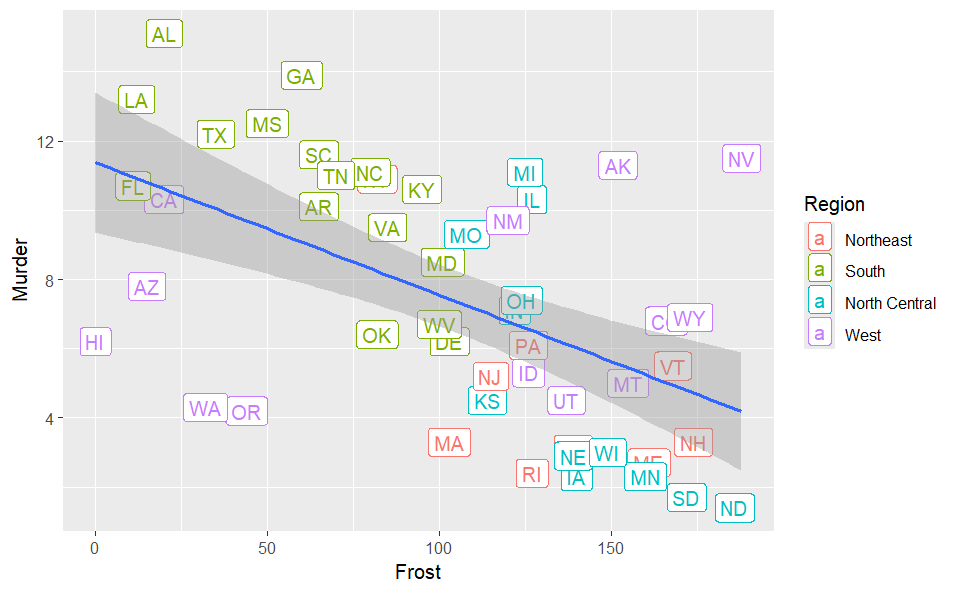
\includegraphics[width=0.75\linewidth]{img/vis.ex9} \end{center}

\end{exercise}

\begin{exercise}

Using the \texttt{soilCO2} data from igisci, create a boxplot arranged by the SITE factor and using a log10 scaling on the y axis displaying soil CO2 values.

\begin{center}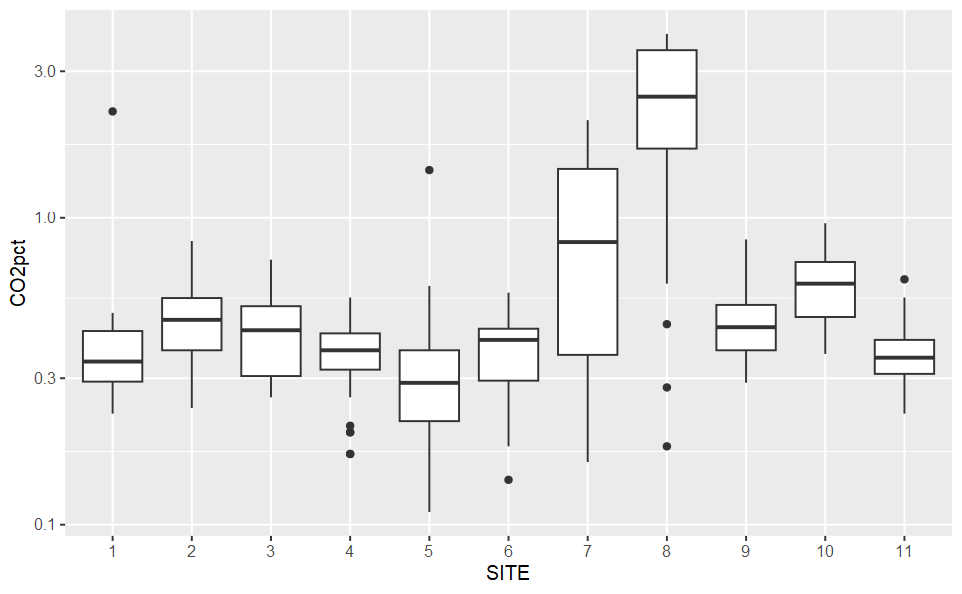
\includegraphics[width=0.75\linewidth]{img/vis.ex10} \end{center}

\end{exercise}

\chapter{Data Transformation}\label{transformation}

\begin{center}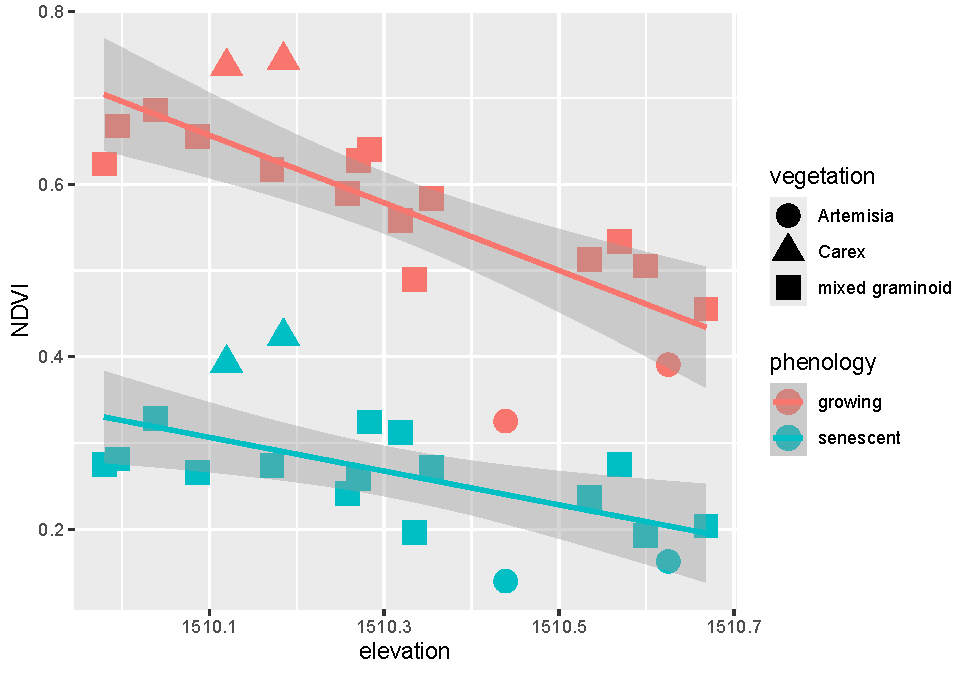
\includegraphics[width=0.75\linewidth]{EnvDataScience_files/figure-latex/Transformation-1} \end{center}

The goal of this section is to continue where we started in the earlier
chapter on data abstraction with \index{dplyr}\textbf{\texttt{dplyr}} to look at the
more transformational functions applied to data in a database, and
\index{tidyr}\textbf{\texttt{tidyr}} adds other tools like pivot tables.

\begin{itemize}
\item
  \textbf{\texttt{dplyr}} tools:

  \begin{itemize}
  \tightlist
  \item
    joins: \texttt{left\_join}, \texttt{right\_join}, \texttt{inner\_join}, \texttt{full\_join},
    \texttt{semi\_join}, \texttt{anti\_join}
  \item
    set operations: \texttt{intersect}, \texttt{union}, \texttt{setdiff}
  \item
    binding rows and columns: \texttt{bind\_cols}, \texttt{bind\_rows}
  \end{itemize}
\item
  \textbf{\texttt{tidyr}} tools:

  \begin{itemize}
  \tightlist
  \item
    pivot tables: \texttt{pivot\_longer}, \texttt{pivot\_wider}
  \end{itemize}
\end{itemize}

The term ``data wrangling'' has been used for what we're doing with these
tools, and the relevant cheat sheet used to be called that, but now they
have names like ``Data transformation with dplyr'' and ``Data tidying with
tidyr'', but those could change too. See what's current at
\url{https://www.rstudio.com/resources/cheatsheets/}

\section{Data joins}\label{joins}

\index{join, data}To bring in variables from another data frame based on
a common join field. There are multiple types of joins. Probably the
most common is \textbf{\texttt{left\_join}} since it starts from the data frame (or
sf) you want to continue working with and bring in data from an
additional source. You'll retain all records of the first data set. For
any non-matches, \texttt{NA} is assigned.

\begin{Shaded}
\begin{Highlighting}[]
\FunctionTok{library}\NormalTok{(tidyverse)}
\FunctionTok{library}\NormalTok{(igisci)}
\FunctionTok{library}\NormalTok{(sf)}
\NormalTok{income }\OtherTok{\textless{}{-}} \FunctionTok{read\_csv}\NormalTok{(}\FunctionTok{ex}\NormalTok{(}\StringTok{"CA/CA\_MdInc.csv"}\NormalTok{)) }\SpecialCharTok{|\textgreater{}}
\NormalTok{   dplyr}\SpecialCharTok{::}\FunctionTok{select}\NormalTok{(trID, HHinc2016) }\SpecialCharTok{|\textgreater{}}
   \FunctionTok{mutate}\NormalTok{(}\AttributeTok{HHinc2016 =} \FunctionTok{as.numeric}\NormalTok{(HHinc2016),}
          \AttributeTok{joinid =} \FunctionTok{str\_c}\NormalTok{(}\StringTok{"0"}\NormalTok{, trID)) }\SpecialCharTok{|\textgreater{}}
\NormalTok{   dplyr}\SpecialCharTok{::}\FunctionTok{select}\NormalTok{(joinid, HHinc2016)}
\NormalTok{census }\OtherTok{\textless{}{-}}\NormalTok{ BayAreaTracts }\SpecialCharTok{|\textgreater{}}
   \FunctionTok{left\_join}\NormalTok{(income, }\AttributeTok{by =} \FunctionTok{c}\NormalTok{(}\StringTok{"FIPS"} \OtherTok{=} \StringTok{"joinid"}\NormalTok{)) }\SpecialCharTok{|\textgreater{}}
\NormalTok{   dplyr}\SpecialCharTok{::}\FunctionTok{select}\NormalTok{(FIPS, POP12\_SQMI, POP2012, HHinc2016)}
\FunctionTok{head}\NormalTok{(census }\SpecialCharTok{|\textgreater{}} \FunctionTok{st\_set\_geometry}\NormalTok{(}\ConstantTok{NULL}\NormalTok{))}
\end{Highlighting}
\end{Shaded}

\begin{verbatim}
##          FIPS POP12_SQMI POP2012 HHinc2016
## 1 06001400100   1118.797    2976    177417
## 2 06001400200   9130.435    2100    153125
## 3 06001400300  11440.476    4805     85313
## 4 06001400400  14573.077    3789     99539
## 5 06001400500  15582.609    3584     83650
## 6 06001400600  13516.667    1622     61597
\end{verbatim}

Other joins are:

\begin{itemize}
\tightlist
\item
  \textbf{\texttt{right\_join}} \index{right\_join}where you end up retaining all
  the rows of the second data set and NA is assigned to non-matches
\item
  \textbf{\texttt{inner\_join}} \index{inner\_join}where you only retain records
  for matches
\item
  \textbf{\texttt{full\_join}} \index{full\_join}where records are retained for
  both sides, and NAs are assigned to non-matches
\end{itemize}

\textbf{Right join example} We need to join NCDC monthly climate data for all
California weather stations to a selection of 82 stations that are in
the Sierra.

\begin{itemize}
\tightlist
\item
  The monthly data has 12 rows (1/month) for each station
\item
  The right\_join gets all months for all stations, so we weed out the
  non-Sierra stations by removing NAs from a field only with Sierra
  station data
\end{itemize}

\begin{Shaded}
\begin{Highlighting}[]
\NormalTok{sierra }\OtherTok{\textless{}{-}} \FunctionTok{right\_join}\NormalTok{(sierraStations, CA\_ClimateNormals, }\AttributeTok{by=}\StringTok{"STATION"}\NormalTok{) }\SpecialCharTok{|\textgreater{}}
   \FunctionTok{filter}\NormalTok{(}\SpecialCharTok{!}\FunctionTok{is.na}\NormalTok{(STATION\_NA)) }\SpecialCharTok{|\textgreater{}}\NormalTok{ dplyr}\SpecialCharTok{::}\FunctionTok{select}\NormalTok{(}\SpecialCharTok{{-}}\NormalTok{STATION\_NA)}
\FunctionTok{head}\NormalTok{(sierra }\SpecialCharTok{|\textgreater{}} \FunctionTok{filter}\NormalTok{(DATE }\SpecialCharTok{==} \StringTok{"01"}\NormalTok{) }\SpecialCharTok{|\textgreater{}} 
\NormalTok{   dplyr}\SpecialCharTok{::}\FunctionTok{select}\NormalTok{(NAME, ELEVATION, }\StringTok{\textasciigrave{}}\AttributeTok{MLY{-}TAVG{-}NORMAL}\StringTok{\textasciigrave{}}\NormalTok{), }\AttributeTok{n=}\DecValTok{10}\NormalTok{)}
\end{Highlighting}
\end{Shaded}

\begin{verbatim}
## # A tibble: 10 x 3
##    NAME                              ELEVATION `MLY-TAVG-NORMAL`
##    <chr>                                 <dbl>             <dbl>
##  1 GROVELAND 2, CA US                    853.                5.6
##  2 CANYON DAM, CA US                    1390.                0.2
##  3 KERN RIVER PH 3, CA US                824.                7.6
##  4 DONNER MEMORIAL ST PARK, CA US       1810.               -1.9
##  5 BOWMAN DAM, CA US                    1641.                3  
##  6 BRUSH CREEK RANGER STATION, CA US    1085.               NA  
##  7 GRANT GROVE, CA US                   2012.                1.9
##  8 LEE VINING, CA US                    2072.               -1.2
##  9 OROVILLE MUNICIPAL AIRPORT, CA US      57.9               7.7
## 10 LEMON COVE, CA US                     156.                8.6
\end{verbatim}

The exact same thing, however, could be accomplished with an inner\_join,
and it doesn't required removing the NAs:

\begin{Shaded}
\begin{Highlighting}[]
\NormalTok{sierraAlso }\OtherTok{\textless{}{-}} \FunctionTok{inner\_join}\NormalTok{(sierraStations, CA\_ClimateNormals, }\AttributeTok{by=}\StringTok{"STATION"}\NormalTok{) }\SpecialCharTok{|\textgreater{}}
\NormalTok{   dplyr}\SpecialCharTok{::}\FunctionTok{select}\NormalTok{(}\SpecialCharTok{{-}}\NormalTok{STATION\_NA)}
\end{Highlighting}
\end{Shaded}

\section{Set operations}\label{set}

\index{set operations}Set operations compare two data frames (or
vectors) to handle observations or rows that are the same for each, or
not the same. The three set methods are:

\begin{itemize}
\tightlist
\item
  \texttt{dplyr::intersect(x,y)} \index{intersect}retains rows that appear in
  \emph{both} x and y
\item
  \texttt{dplyr::union(x,y)} \index{union}retains rows that appear in either
  or both of x and y
\item
  \texttt{dplyr::setdiff(x,y)} \index{setdiff}retains rows that appear in x
  but not in y
\end{itemize}

\begin{Shaded}
\begin{Highlighting}[]
\NormalTok{squares }\OtherTok{\textless{}{-}}\NormalTok{ (}\DecValTok{1}\SpecialCharTok{:}\DecValTok{10}\NormalTok{)}\SpecialCharTok{\^{}}\DecValTok{2}
\NormalTok{evens }\OtherTok{\textless{}{-}} \FunctionTok{seq}\NormalTok{(}\DecValTok{0}\NormalTok{,}\DecValTok{100}\NormalTok{,}\DecValTok{2}\NormalTok{)}
\NormalTok{squares}
\end{Highlighting}
\end{Shaded}

\begin{verbatim}
##  [1]   1   4   9  16  25  36  49  64  81 100
\end{verbatim}

\begin{Shaded}
\begin{Highlighting}[]
\NormalTok{evens}
\end{Highlighting}
\end{Shaded}

\begin{verbatim}
##  [1]   0   2   4   6   8  10  12  14  16  18  20  22  24  26  28  30  32  34  36
## [20]  38  40  42  44  46  48  50  52  54  56  58  60  62  64  66  68  70  72  74
## [39]  76  78  80  82  84  86  88  90  92  94  96  98 100
\end{verbatim}

\begin{Shaded}
\begin{Highlighting}[]
\FunctionTok{intersect}\NormalTok{(squares,evens)}
\end{Highlighting}
\end{Shaded}

\begin{verbatim}
## [1]   4  16  36  64 100
\end{verbatim}

\begin{Shaded}
\begin{Highlighting}[]
\FunctionTok{sort}\NormalTok{(}\FunctionTok{union}\NormalTok{(squares,evens))}
\end{Highlighting}
\end{Shaded}

\begin{verbatim}
##  [1]   0   1   2   4   6   8   9  10  12  14  16  18  20  22  24  25  26  28  30
## [20]  32  34  36  38  40  42  44  46  48  49  50  52  54  56  58  60  62  64  66
## [39]  68  70  72  74  76  78  80  81  82  84  86  88  90  92  94  96  98 100
\end{verbatim}

\begin{Shaded}
\begin{Highlighting}[]
\FunctionTok{sort}\NormalTok{(}\FunctionTok{setdiff}\NormalTok{(squares,evens))}
\end{Highlighting}
\end{Shaded}

\begin{verbatim}
## [1]  1  9 25 49 81
\end{verbatim}

\section{Binding rows and columns}\label{binding}

\index{bind\_cols}\index{bind\_rows}These \texttt{dplyr} functions are similar
to \texttt{cbind} and \texttt{rbind} in base R, but always create data frames. For
instance, \texttt{cbind} usually creates matrices and makes all vectors the
same class. Note that in \texttt{bind\_cols}, the order of data in rows must be
the same.

\begin{Shaded}
\begin{Highlighting}[]
\NormalTok{states }\OtherTok{\textless{}{-}} \FunctionTok{bind\_cols}\NormalTok{(}\AttributeTok{abb=}\NormalTok{state.abb,}
                    \AttributeTok{name=}\NormalTok{state.name,}
                    \AttributeTok{region=}\NormalTok{state.region,}
\NormalTok{                    state.x77)}
\FunctionTok{head}\NormalTok{(states)}
\end{Highlighting}
\end{Shaded}

\begin{verbatim}
## # A tibble: 6 x 11
##   abb   name     region Population Income Illiteracy `Life Exp` Murder `HS Grad`
##   <chr> <chr>    <fct>       <dbl>  <dbl>      <dbl>      <dbl>  <dbl>     <dbl>
## 1 AL    Alabama  South        3615   3624        2.1       69.0   15.1      41.3
## 2 AK    Alaska   West          365   6315        1.5       69.3   11.3      66.7
## 3 AZ    Arizona  West         2212   4530        1.8       70.6    7.8      58.1
## 4 AR    Arkansas South        2110   3378        1.9       70.7   10.1      39.9
## 5 CA    Califor~ West        21198   5114        1.1       71.7   10.3      62.6
## 6 CO    Colorado West         2541   4884        0.7       72.1    6.8      63.9
## # i 2 more variables: Frost <dbl>, Area <dbl>
\end{verbatim}

To compare, note that \texttt{cbind} converts numeric fields to character type
when any other field is character, and character fields are converted to
character integers where there are any repeats, which would require
manipulating them into factors:

\begin{Shaded}
\begin{Highlighting}[]
\NormalTok{states }\OtherTok{\textless{}{-}} \FunctionTok{as\_tibble}\NormalTok{(}\FunctionTok{cbind}\NormalTok{(}\AttributeTok{abb=}\NormalTok{state.abb, }
                          \AttributeTok{name=}\NormalTok{state.name, }
                          \AttributeTok{region=}\NormalTok{state.region,}
                          \AttributeTok{division=}\NormalTok{state.division,}
\NormalTok{                          state.x77))}
\FunctionTok{head}\NormalTok{(states)}
\end{Highlighting}
\end{Shaded}

\begin{verbatim}
## # A tibble: 6 x 12
##   abb   name      region division Population Income Illiteracy `Life Exp` Murder
##   <chr> <chr>     <chr>  <chr>    <chr>      <chr>  <chr>      <chr>      <chr> 
## 1 AL    Alabama   2      4        3615       3624   2.1        69.05      15.1  
## 2 AK    Alaska    4      9        365        6315   1.5        69.31      11.3  
## 3 AZ    Arizona   4      8        2212       4530   1.8        70.55      7.8   
## 4 AR    Arkansas  2      5        2110       3378   1.9        70.66      10.1  
## 5 CA    Californ~ 4      9        21198      5114   1.1        71.71      10.3  
## 6 CO    Colorado  4      8        2541       4884   0.7        72.06      6.8   
## # i 3 more variables: `HS Grad` <chr>, Frost <chr>, Area <chr>
\end{verbatim}

\section{Pivoting data frames}\label{pivots}

\index{pivoting}Pivot tables are a popular tool in Excel, allowing you
to transform your data to be more useful in a particular analysis. A
common need to pivot is 2+ variables with the same data where the
variable name should be a factor. \texttt{Tidyr} has \textbf{\texttt{pivot\_wider}} and
\textbf{\texttt{pivot\_longer}}.

\begin{itemize}
\tightlist
\item
  \textbf{\texttt{pivot\_wider}} \index{pivot\_wider}pivots rows into variables.
\item
  \textbf{\texttt{pivot\_longer}} \index{pivot\_longer}pivots variables into rows,
  creating factors.
\end{itemize}

\subsection{\texorpdfstring{\texttt{pivot\_longer}}{pivot\_longer}}\label{pivot_longer}

In our meadows study cross-section (\citeproc{ref-NDVI}{Davis et al. 2020}) created by intersecting
normalized difference vegetation index (NDVI) values from multispectral
drone imagery with surveyed elevation and vegetation types (xeric,
mesic, and hydric), we have fields \texttt{NDVIgrowing} from a July 2019
growing season and \texttt{NDVIsenescent} from a September 2020 dry season, but
would like ``growing'' and ``senescent'' to be factors with a single \texttt{NDVI}
variable. This is how we used \texttt{pivot\_longer} to accomplish this, using
data from the \texttt{igisci} data package:

\begin{Shaded}
\begin{Highlighting}[]
\NormalTok{XSptsPheno }\OtherTok{\textless{}{-}}\NormalTok{ XSptsNDVI }\SpecialCharTok{|\textgreater{}}
      \FunctionTok{filter}\NormalTok{(vegetation }\SpecialCharTok{!=} \StringTok{"pine"}\NormalTok{) }\SpecialCharTok{|\textgreater{}}    \CommentTok{\# trees removed}
      \FunctionTok{pivot\_longer}\NormalTok{(}\AttributeTok{cols =} \FunctionTok{starts\_with}\NormalTok{(}\StringTok{"NDVI"}\NormalTok{), }
                   \AttributeTok{names\_to =} \StringTok{"phenology"}\NormalTok{, }\AttributeTok{values\_to =} \StringTok{"NDVI"}\NormalTok{) }\SpecialCharTok{|\textgreater{}}
      \FunctionTok{mutate}\NormalTok{(}\AttributeTok{phenology =} \FunctionTok{str\_sub}\NormalTok{(phenology, }\DecValTok{5}\NormalTok{, }\FunctionTok{str\_length}\NormalTok{(phenology)))}
\end{Highlighting}
\end{Shaded}

To see what the reverse would be, we'd use \texttt{pivot\_wider} to return to
the original, but note that we're not writing over our \texttt{XSptsPheno} data
frame.

\begin{Shaded}
\begin{Highlighting}[]
\NormalTok{XSptsPheno }\SpecialCharTok{|\textgreater{}}
  \FunctionTok{pivot\_wider}\NormalTok{(}\AttributeTok{names\_from =}\NormalTok{ phenology, }\AttributeTok{names\_prefix =} \StringTok{"NDVI"}\NormalTok{, }
              \AttributeTok{values\_from =}\NormalTok{ NDVI)}
\end{Highlighting}
\end{Shaded}

\begin{verbatim}
## # A tibble: 19 x 6
##    DistNtoS elevation vegetation      geometry         NDVIgrowing NDVIsenescent
##       <dbl>     <dbl> <chr>           <chr>                  <dbl>         <dbl>
##  1      0       1510. Artemisia       c(718649.456, 4~       0.326         0.140
##  2     16.7     1510. mixed graminoid c(718649.4309, ~       0.627         0.259
##  3     28.6     1510. mixed graminoid c(718649.413, 4~       0.686         0.329
##  4     30.5     1510. mixed graminoid c(718649.4101, ~       0.668         0.282
##  5     31.1     1510. mixed graminoid c(718649.4092, ~       0.655         0.266
##  6     33.4     1510. mixed graminoid c(718649.4058, ~       0.617         0.274
##  7     35.6     1510. mixed graminoid c(718649.4025, ~       0.623         0.275
##  8     37       1510. mixed graminoid c(718649.4004, ~       0.589         0.242
##  9     74       1510. mixed graminoid c(718649.3448, ~       0.641         0.325
## 10    101       1510. mixed graminoid c(718649.3042, ~       0.558         0.312
## 11    126.      1511. Artemisia       c(718649.2672, ~       0.391         0.163
## 12    137       1510. mixed graminoid c(718649.25, 43~       0.583         0.272
## 13    149.      1510. Carex           c(718649.2317, ~       0.736         0.392
## 14    154.      1510. Carex           c(718649.224, 4~       0.744         0.424
## 15    175       1511. mixed graminoid c(718649.1929, ~       0.455         0.204
## 16    195.      1511. mixed graminoid c(718649.1633, ~       0.512         0.237
## 17    197.      1510. mixed graminoid c(718649.1597, ~       0.489         0.197
## 18    201.      1511. mixed graminoid c(718649.1544, ~       0.533         0.275
## 19    259.      1511. mixed graminoid c(718649.0663, ~       0.505         0.193
\end{verbatim}

\begin{Shaded}
\begin{Highlighting}[]
\NormalTok{XSptsPheno}
\end{Highlighting}
\end{Shaded}

\begin{verbatim}
## # A tibble: 38 x 6
##    DistNtoS elevation vegetation      geometry                   phenology  NDVI
##       <dbl>     <dbl> <chr>           <chr>                      <chr>     <dbl>
##  1      0       1510. Artemisia       c(718649.456, 4397466.714) growing   0.326
##  2      0       1510. Artemisia       c(718649.456, 4397466.714) senescent 0.140
##  3     16.7     1510. mixed graminoid c(718649.4309, 4397450.07~ growing   0.627
##  4     16.7     1510. mixed graminoid c(718649.4309, 4397450.07~ senescent 0.259
##  5     28.6     1510. mixed graminoid c(718649.413, 4397438.222) growing   0.686
##  6     28.6     1510. mixed graminoid c(718649.413, 4397438.222) senescent 0.329
##  7     30.5     1510. mixed graminoid c(718649.4101, 4397436.33) growing   0.668
##  8     30.5     1510. mixed graminoid c(718649.4101, 4397436.33) senescent 0.282
##  9     31.1     1510. mixed graminoid c(718649.4092, 4397435.73~ growing   0.655
## 10     31.1     1510. mixed graminoid c(718649.4092, 4397435.73~ senescent 0.266
## # i 28 more rows
\end{verbatim}

We'll use the \texttt{pivot\_longer} result (the one we actually assigned to
\texttt{XSptsPheno}) to allow us to create the graph we're after (Figure
\ref{fig:transPivotPheno}).

\begin{Shaded}
\begin{Highlighting}[]
\NormalTok{XSptsPheno }\SpecialCharTok{|\textgreater{}}
  \FunctionTok{ggplot}\NormalTok{() }\SpecialCharTok{+}
  \FunctionTok{geom\_point}\NormalTok{(}\FunctionTok{aes}\NormalTok{(elevation, NDVI, }\AttributeTok{shape=}\NormalTok{vegetation, }
                 \AttributeTok{color =}\NormalTok{ phenology), }\AttributeTok{size =} \DecValTok{5}\NormalTok{) }\SpecialCharTok{+}
  \FunctionTok{geom\_smooth}\NormalTok{(}\FunctionTok{aes}\NormalTok{(elevation, NDVI, }
                 \AttributeTok{color =}\NormalTok{ phenology), }\AttributeTok{method=}\StringTok{"lm"}\NormalTok{)}
\end{Highlighting}
\end{Shaded}

\begin{figure}

{\centering 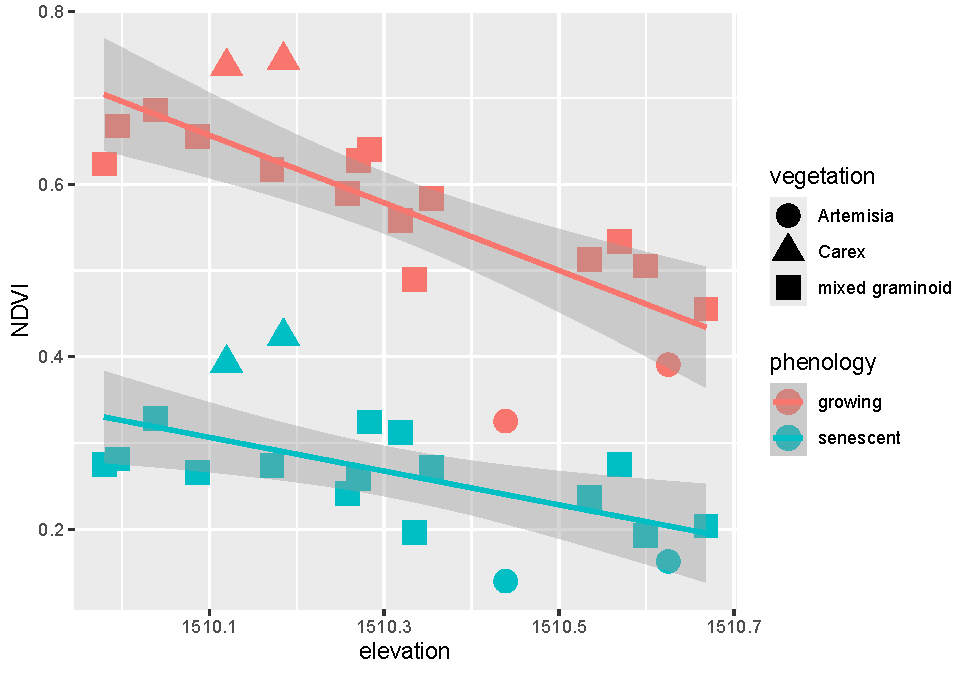
\includegraphics[width=0.75\linewidth]{EnvDataScience_files/figure-latex/transPivotPheno-1} 

}

\caption{Color classified by phenology, data created by a pivot}\label{fig:transPivotPheno}
\end{figure}

Pivots turn out to be commonly useful. We've already seen their use in
the Visualization chapter, such as when we graphed runoff from the
Eucalyptus/Oak study (\citeproc{ref-eucoak}{Thompson et al. 2016}), where we used a \texttt{pivot\_longer} (Figure
\ref{fig:transEucOakPivot}).

\begin{Shaded}
\begin{Highlighting}[]
\NormalTok{eucoakrainfallrunoffTDR }\SpecialCharTok{|\textgreater{}}
  \FunctionTok{pivot\_longer}\NormalTok{(}\AttributeTok{cols =} \FunctionTok{starts\_with}\NormalTok{(}\StringTok{"runoffL"}\NormalTok{),}
               \AttributeTok{names\_to =} \StringTok{"tree"}\NormalTok{, }\AttributeTok{values\_to =} \StringTok{"runoffL"}\NormalTok{) }\SpecialCharTok{|\textgreater{}}
  \FunctionTok{mutate}\NormalTok{(}\AttributeTok{tree =} \FunctionTok{str\_sub}\NormalTok{(tree, }\FunctionTok{str\_length}\NormalTok{(tree)}\SpecialCharTok{{-}}\DecValTok{2}\NormalTok{, }\FunctionTok{str\_length}\NormalTok{(tree))) }\SpecialCharTok{|\textgreater{}}
  \FunctionTok{ggplot}\NormalTok{() }\SpecialCharTok{+} \FunctionTok{geom\_boxplot}\NormalTok{(}\FunctionTok{aes}\NormalTok{(site, runoffL)) }\SpecialCharTok{+}
    \FunctionTok{facet\_grid}\NormalTok{(tree }\SpecialCharTok{\textasciitilde{}}\NormalTok{ .)}
\end{Highlighting}
\end{Shaded}

\begin{figure}

{\centering 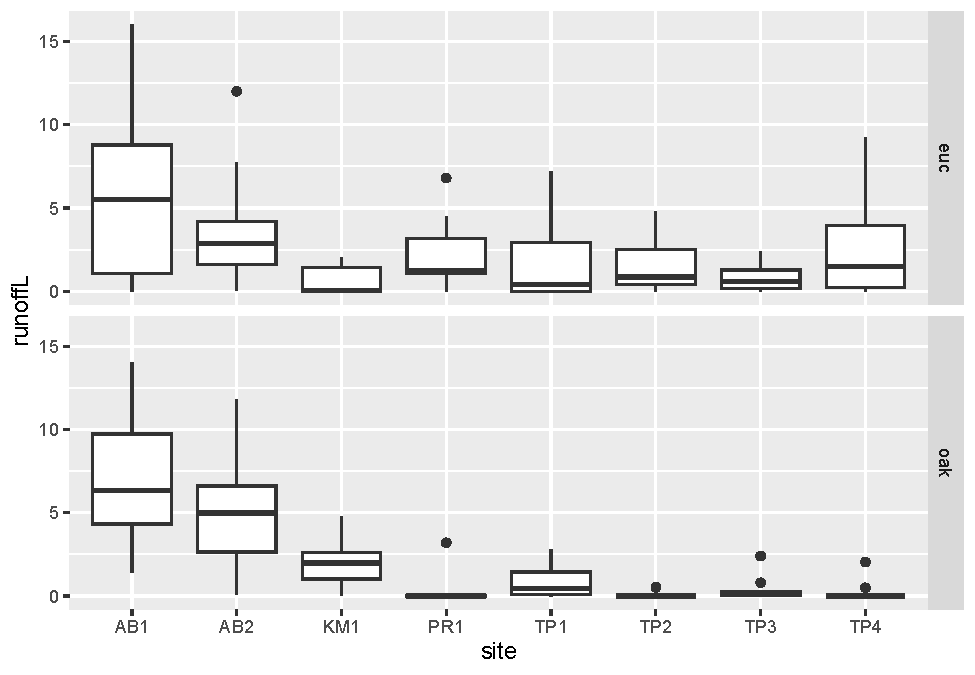
\includegraphics[width=0.75\linewidth]{EnvDataScience_files/figure-latex/transEucOakPivot-1} 

}

\caption{Euc vs oak graphs created using a pivot}\label{fig:transEucOakPivot}
\end{figure}

\textbf{Combining a pivot with bind\_rows to create a runoff/rainfall
scatterplot colored by tree}

With a bit more code, we can combine pivoting with binding rows to set
up a useful scatter plot (Figure \ref{fig:transEucOakScatterplot}).

\begin{Shaded}
\begin{Highlighting}[]
\NormalTok{runoffPivot }\OtherTok{\textless{}{-}}\NormalTok{ eucoakrainfallrunoffTDR }\SpecialCharTok{|\textgreater{}}
  \FunctionTok{pivot\_longer}\NormalTok{(}\AttributeTok{cols =} \FunctionTok{starts\_with}\NormalTok{(}\StringTok{"runoffL"}\NormalTok{),}
               \AttributeTok{names\_to =} \StringTok{"tree"}\NormalTok{, }\AttributeTok{values\_to =} \StringTok{"runoffL"}\NormalTok{) }\SpecialCharTok{|\textgreater{}}
  \FunctionTok{mutate}\NormalTok{(}\AttributeTok{tree =} \FunctionTok{str\_sub}\NormalTok{(tree, }\FunctionTok{str\_length}\NormalTok{(tree)}\SpecialCharTok{{-}}\DecValTok{2}\NormalTok{, }\FunctionTok{str\_length}\NormalTok{(tree)),}
         \AttributeTok{Date =} \FunctionTok{as.Date}\NormalTok{(date, }\StringTok{"\%m/\%d/\%Y"}\NormalTok{))}
\NormalTok{euc }\OtherTok{\textless{}{-}}\NormalTok{ runoffPivot }\SpecialCharTok{|\textgreater{}}
  \FunctionTok{filter}\NormalTok{(tree }\SpecialCharTok{==} \StringTok{"euc"}\NormalTok{) }\SpecialCharTok{|\textgreater{}}
  \FunctionTok{mutate}\NormalTok{(}\AttributeTok{rain\_subcanopy =}\NormalTok{ rain\_euc,}
         \AttributeTok{slope =}\NormalTok{ slope\_euc,    }\AttributeTok{aspect =}\NormalTok{ aspect\_euc,}
         \AttributeTok{surface\_tension =}\NormalTok{ surface\_tension\_euc,}
         \AttributeTok{runoff\_rainfall\_ratio =}\NormalTok{ runoff\_rainfall\_ratio\_euc) }\SpecialCharTok{|\textgreater{}}
\NormalTok{  dplyr}\SpecialCharTok{::}\FunctionTok{select}\NormalTok{(site, }\StringTok{\textasciigrave{}}\AttributeTok{site \#}\StringTok{\textasciigrave{}}\NormalTok{, tree, Date, month, rain\_mm, }
\NormalTok{         rain\_subcanopy, slope, aspect, runoffL,     }
\NormalTok{         surface\_tension, runoff\_rainfall\_ratio)}
\NormalTok{oak }\OtherTok{\textless{}{-}}\NormalTok{ runoffPivot }\SpecialCharTok{|\textgreater{}}
  \FunctionTok{filter}\NormalTok{(tree }\SpecialCharTok{==} \StringTok{"oak"}\NormalTok{) }\SpecialCharTok{|\textgreater{}}
  \FunctionTok{mutate}\NormalTok{(}\AttributeTok{rain\_subcanopy =}\NormalTok{ rain\_oak,}
         \AttributeTok{slope =}\NormalTok{ slope\_oak, }\AttributeTok{aspect =}\NormalTok{ aspect\_oak,}
         \AttributeTok{surface\_tension =}\NormalTok{ surface\_tension\_oak,}
         \AttributeTok{runoff\_rainfall\_ratio =}\NormalTok{ runoff\_rainfall\_ratio\_oak) }\SpecialCharTok{|\textgreater{}}
\NormalTok{  dplyr}\SpecialCharTok{::}\FunctionTok{select}\NormalTok{(site, }\StringTok{\textasciigrave{}}\AttributeTok{site \#}\StringTok{\textasciigrave{}}\NormalTok{, tree, Date, month, rain\_mm, }
\NormalTok{         rain\_subcanopy, slope, aspect, runoffL, }
\NormalTok{         surface\_tension, runoff\_rainfall\_ratio)}
\FunctionTok{bind\_rows}\NormalTok{(euc, oak) }\SpecialCharTok{|\textgreater{}}
  \FunctionTok{ggplot}\NormalTok{() }\SpecialCharTok{+}
  \FunctionTok{geom\_point}\NormalTok{(}\AttributeTok{mapping =} \FunctionTok{aes}\NormalTok{(}\AttributeTok{x =}\NormalTok{ rain\_mm, }\AttributeTok{y =}\NormalTok{ runoffL, }\AttributeTok{color =}\NormalTok{ tree)) }\SpecialCharTok{+}
  \FunctionTok{geom\_smooth}\NormalTok{(}\AttributeTok{mapping =} \FunctionTok{aes}\NormalTok{(}\AttributeTok{x =}\NormalTok{ rain\_mm, }\AttributeTok{y=}\NormalTok{ runoffL, }\AttributeTok{color =}\NormalTok{ tree), }
              \AttributeTok{method =} \StringTok{"lm"}\NormalTok{) }\SpecialCharTok{+}
  \FunctionTok{scale\_color\_manual}\NormalTok{(}\AttributeTok{values =} \FunctionTok{c}\NormalTok{(}\StringTok{"seagreen4"}\NormalTok{, }\StringTok{"orange3"}\NormalTok{))}
\end{Highlighting}
\end{Shaded}

\begin{figure}

{\centering 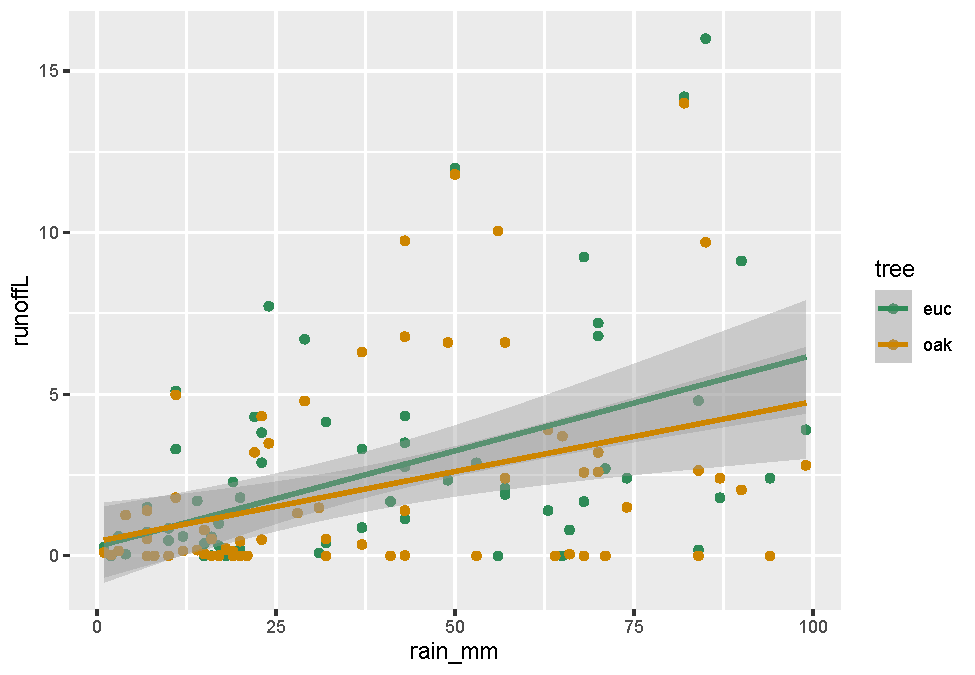
\includegraphics[width=0.75\linewidth]{EnvDataScience_files/figure-latex/transEucOakScatterplot-1} 

}

\caption{Runoff/rainfall scatterplot colored by tree, created by pivot and binding rows}\label{fig:transEucOakScatterplot}
\end{figure}

\subsection{\texorpdfstring{\texttt{pivot\_wider}}{pivot\_wider}}\label{pivot_wider}

\index{pivot\_wider}The opposite of \texttt{pivot\_longer}, \texttt{pivot\_wider} is
less commonly used for tidying data, but can be useful for creating
tables of that desired format. An environmental application of
\texttt{pivot\_wider} can be found in \texttt{vignette("pivot")} (modified below) for
studying fish detected by automatic monitors, with \texttt{fish\_encounters}
data contributed by Johnston and Rudis (\citeproc{ref-JohnstonRudis}{n.d.}) . This pivot makes it easier to see
fish encounters by station. See Johnston and Rudis (\citeproc{ref-JohnstonRudis}{n.d.}) and \texttt{vignette("pivot")}
for more information on the dataset and how the pivot provides this
view.

\begin{Shaded}
\begin{Highlighting}[]
\FunctionTok{library}\NormalTok{(tidyverse)}
\NormalTok{fish\_encounters }\OtherTok{\textless{}{-}} \FunctionTok{read\_csv}\NormalTok{(}\FunctionTok{ex}\NormalTok{(}\StringTok{"fishdata.csv"}\NormalTok{))}
\NormalTok{fish\_encounters}
\end{Highlighting}
\end{Shaded}

\begin{verbatim}
## # A tibble: 209 x 3
##    TagID Station value
##    <dbl> <chr>   <dbl>
##  1  4842 Release     1
##  2  4843 Release     1
##  3  4844 Release     1
##  4  4845 Release     1
##  5  4847 Release     1
##  6  4848 Release     1
##  7  4849 Release     1
##  8  4850 Release     1
##  9  4851 Release     1
## 10  4854 Release     1
## # i 199 more rows
\end{verbatim}

\begin{Shaded}
\begin{Highlighting}[]
\NormalTok{fishEncountersWide }\OtherTok{\textless{}{-}}\NormalTok{ fish\_encounters }\SpecialCharTok{|\textgreater{}} 
  \FunctionTok{pivot\_wider}\NormalTok{(}\AttributeTok{names\_from =}\NormalTok{ Station, }\AttributeTok{values\_from =}\NormalTok{ value, }\AttributeTok{values\_fill =} \DecValTok{0}\NormalTok{)}
\NormalTok{fishEncountersWide}
\end{Highlighting}
\end{Shaded}

\begin{verbatim}
## # A tibble: 19 x 12
##    TagID Release I80_1 Lisbon  Rstr Base_TD   BCE   BCW  BCE2  BCW2   MAE   MAW
##    <dbl>   <dbl> <dbl>  <dbl> <dbl>   <dbl> <dbl> <dbl> <dbl> <dbl> <dbl> <dbl>
##  1  4842       1     1      1     1       1     1     1     1     1     1     1
##  2  4843       1     1      1     1       1     1     1     1     1     1     1
##  3  4844       1     1      1     1       1     1     1     1     1     1     1
##  4  4845       1     1      1     1       1     0     0     0     0     0     0
##  5  4847       1     1      1     0       0     0     0     0     0     0     0
##  6  4848       1     1      1     1       0     0     0     0     0     0     0
##  7  4849       1     1      0     0       0     0     0     0     0     0     0
##  8  4850       1     1      0     1       1     1     1     0     0     0     0
##  9  4851       1     1      0     0       0     0     0     0     0     0     0
## 10  4854       1     1      0     0       0     0     0     0     0     0     0
## 11  4855       1     1      1     1       1     0     0     0     0     0     0
## 12  4857       1     1      1     1       1     1     1     1     1     0     0
## 13  4858       1     1      1     1       1     1     1     1     1     1     1
## 14  4859       1     1      1     1       1     0     0     0     0     0     0
## 15  4861       1     1      1     1       1     1     1     1     1     1     1
## 16  4862       1     1      1     1       1     1     1     1     1     0     0
## 17  4863       1     1      0     0       0     0     0     0     0     0     0
## 18  4864       1     1      0     0       0     0     0     0     0     0     0
## 19  4865       1     1      1     0       0     0     0     0     0     0     0
\end{verbatim}

\section{\texorpdfstring{Combining transformation methods to create a \texttt{free\_y} faceted graph}{Combining transformation methods to create a free\_y faceted graph}}\label{combining-transformation-methods-to-create-a-free_y-faceted-graph}

\index{faceted graph using a pivot}Creating parallel multi-parameter
graphs over a time series can be challenging. We need to link the graphs
with a common x axis, but we may need to vary the scaling on the y axis,
unlike the faceted graph of grouped data we looked at in the
visualization chapter. We'll look at time series in a later chapter, but
this is a good time to explore the use of a pivot\_longer to set up the
data for a graph like this, and at the same time to expand upon our
visualization toolkit.

\subsection{Air pollutant emissions trends (EPA)}\label{air-pollutant-emissions-trends-epa}

The National Emissions Inventory (NEI) program of the US EPA is a
detailed estimate of air emissions of criteria and hazardous air
pollutants from a wide variety of air emissions sources. The inventory
is released every three years based primarily upon data provided by
state, local, and tribal air resources agencies for pollution sources
they monitor, supplemented by data developed by the US EPA.

Air pollutant data was downloaded from
\url{https://www.epa.gov/air-emissions-inventories/air-pollutant-emissions-trends-data}
and provided in the \texttt{igisci} package.

Processing this data to create a \texttt{free\_y} faceted graph employs several
data transformation methods we've looked at, and some details and tricks
we haven't covered:

\begin{itemize}
\tightlist
\item
  \texttt{summarize\_all} gets means of \emph{all} variables, though since we're
  just using the totals, this just causes worksheets with multiple
  \texttt{Total} rows to merge into one; they're actually the same value
\item
  \texttt{pivot\_longer} is used twice, first to create columns for each
  pollutant, so the columns can be bound together, then later to
  create a facet graph where each pollutant becomes a parameter factor
\item
  \texttt{bind\_cols} to combine a series of data frames with each having the
  same years (1990:2016) when data for all parameters were collected
\item
  A fix for dealing data not all being read in as numeric, needed for
  an entry error for the NH3 data, was developed by first reading in
  the \texttt{Source\ Category} column, then the yearly data values, setting
  \texttt{col\_types="numeric"}, then binding the columns
\item
  Using a character string variable to store a pollutant name that can
  be passed to a function and used to access a worksheet, a variable,
  and part of other variables: see how \texttt{pollutant} is used for
  multiple purposes in the function, and how this option of using a
  character string for a variable name is a handy alternative
\end{itemize}

\begin{Shaded}
\begin{Highlighting}[]
\FunctionTok{library}\NormalTok{(tidyverse); }\FunctionTok{library}\NormalTok{(readxl); }\FunctionTok{library}\NormalTok{(igisci)}
\NormalTok{dtaPath }\OtherTok{\textless{}{-}} \FunctionTok{ex}\NormalTok{(}\StringTok{"airquality/Pollution by type US 1970 to 2016.xlsx"}\NormalTok{)}
\NormalTok{YearColumn }\OtherTok{\textless{}{-}}\NormalTok{ readxl}\SpecialCharTok{::}\FunctionTok{read\_xlsx}\NormalTok{(dtaPath, }\AttributeTok{sheet =} \StringTok{"SO2"}\NormalTok{, }\AttributeTok{skip=}\DecValTok{2}\NormalTok{) }\SpecialCharTok{|\textgreater{}}
  \FunctionTok{pivot\_longer}\NormalTok{(}\AttributeTok{cols=}\StringTok{\textasciigrave{}}\AttributeTok{1990}\StringTok{\textasciigrave{}}\SpecialCharTok{:}\StringTok{\textasciigrave{}}\AttributeTok{2016}\StringTok{\textasciigrave{}}\NormalTok{, }\AttributeTok{names\_to=}\StringTok{"Year"}\NormalTok{) }\SpecialCharTok{|\textgreater{}}
\NormalTok{  dplyr}\SpecialCharTok{::}\FunctionTok{select}\NormalTok{(Year) }\SpecialCharTok{|\textgreater{}} \FunctionTok{mutate}\NormalTok{(}\AttributeTok{Year=}\FunctionTok{as.numeric}\NormalTok{(Year))}
\NormalTok{YearCol }\OtherTok{\textless{}{-}} \FunctionTok{as.data.frame}\NormalTok{(}\FunctionTok{unique}\NormalTok{(YearColumn}\SpecialCharTok{$}\NormalTok{Year))}
\FunctionTok{names}\NormalTok{(YearCol) }\OtherTok{=} \StringTok{"Year"}

\NormalTok{getPollutant }\OtherTok{\textless{}{-}} \ControlFlowTok{function}\NormalTok{(pollutant)\{}
\NormalTok{  thedata }\OtherTok{\textless{}{-}}\NormalTok{ readxl}\SpecialCharTok{::}\FunctionTok{read\_xlsx}\NormalTok{(dtaPath,}\AttributeTok{sheet=}\NormalTok{pollutant,}\AttributeTok{skip=}\DecValTok{2}\NormalTok{,}
                               \AttributeTok{col\_types=}\StringTok{"numeric"}\NormalTok{) }\SpecialCharTok{|\textgreater{}}
\NormalTok{     dplyr}\SpecialCharTok{::}\FunctionTok{select}\NormalTok{(}\SpecialCharTok{{-}}\StringTok{\textasciigrave{}}\AttributeTok{Source Category}\StringTok{\textasciigrave{}}\NormalTok{)}
\NormalTok{  rowheaders }\OtherTok{\textless{}{-}}\NormalTok{ readxl}\SpecialCharTok{::}\FunctionTok{read\_xlsx}\NormalTok{(dtaPath,}\AttributeTok{sheet=}\NormalTok{pollutant,}\AttributeTok{skip=}\DecValTok{2}\NormalTok{) }\SpecialCharTok{|\textgreater{}}
\NormalTok{     dplyr}\SpecialCharTok{::}\FunctionTok{select}\NormalTok{(}\StringTok{\textasciigrave{}}\AttributeTok{Source Category}\StringTok{\textasciigrave{}}\NormalTok{)}
  \FunctionTok{bind\_cols}\NormalTok{(rowheaders,thedata) }\SpecialCharTok{|\textgreater{}}
\NormalTok{     dplyr}\SpecialCharTok{::}\FunctionTok{select}\NormalTok{(}\StringTok{\textasciigrave{}}\AttributeTok{Source Category}\StringTok{\textasciigrave{}}\NormalTok{,}\StringTok{\textasciigrave{}}\AttributeTok{1990}\StringTok{\textasciigrave{}}\SpecialCharTok{:}\StringTok{\textasciigrave{}}\AttributeTok{2016}\StringTok{\textasciigrave{}}\NormalTok{) }\SpecialCharTok{|\textgreater{}}
     \FunctionTok{filter}\NormalTok{(}\StringTok{\textasciigrave{}}\AttributeTok{Source Category}\StringTok{\textasciigrave{}}\SpecialCharTok{==}\StringTok{"Total"}\NormalTok{) }\SpecialCharTok{|\textgreater{}}
     \FunctionTok{group\_by}\NormalTok{(}\StringTok{\textasciigrave{}}\AttributeTok{Source Category}\StringTok{\textasciigrave{}}\NormalTok{) }\SpecialCharTok{|\textgreater{}}
     \FunctionTok{summarize\_all}\NormalTok{(}\FunctionTok{list}\NormalTok{(mean)) }\SpecialCharTok{|\textgreater{}}
     \FunctionTok{pivot\_longer}\NormalTok{(}\AttributeTok{cols=}\StringTok{\textasciigrave{}}\AttributeTok{1990}\StringTok{\textasciigrave{}}\SpecialCharTok{:}\StringTok{\textasciigrave{}}\AttributeTok{2016}\StringTok{\textasciigrave{}}\NormalTok{,}\AttributeTok{names\_to=}\StringTok{"Year"}\NormalTok{,}\AttributeTok{values\_to=}\NormalTok{pollutant) }\SpecialCharTok{|\textgreater{}}
\NormalTok{     dplyr}\SpecialCharTok{::}\FunctionTok{select}\NormalTok{(pollutant)}
\NormalTok{\}}
\NormalTok{SO2  }\OtherTok{\textless{}{-}} \FunctionTok{getPollutant}\NormalTok{(}\StringTok{"SO2"}\NormalTok{)}
\NormalTok{PM25 }\OtherTok{\textless{}{-}} \FunctionTok{getPollutant}\NormalTok{(}\StringTok{"PM25Primary"}\NormalTok{) }\SpecialCharTok{|\textgreater{}} \FunctionTok{rename}\NormalTok{(}\AttributeTok{PM25=}\NormalTok{PM25Primary)}
\NormalTok{PM10 }\OtherTok{\textless{}{-}} \FunctionTok{getPollutant}\NormalTok{(}\StringTok{"PM10Primary"}\NormalTok{) }\SpecialCharTok{|\textgreater{}} \FunctionTok{rename}\NormalTok{(}\AttributeTok{PM10=}\NormalTok{PM10Primary)}
\NormalTok{NOX  }\OtherTok{\textless{}{-}} \FunctionTok{getPollutant}\NormalTok{(}\StringTok{"NOX"}\NormalTok{)}
\NormalTok{CO   }\OtherTok{\textless{}{-}} \FunctionTok{getPollutant}\NormalTok{(}\StringTok{"CO"}\NormalTok{)}
\NormalTok{VOC  }\OtherTok{\textless{}{-}} \FunctionTok{getPollutant}\NormalTok{(}\StringTok{"VOC"}\NormalTok{)}
\NormalTok{NH3  }\OtherTok{\textless{}{-}} \FunctionTok{getPollutant}\NormalTok{(}\StringTok{"NH3"}\NormalTok{)}
\NormalTok{pollutants }\OtherTok{\textless{}{-}} \FunctionTok{bind\_cols}\NormalTok{(YearCol,CO,NOX,SO2,PM25,PM10,VOC,NH3)}\CommentTok{\#}
\end{Highlighting}
\end{Shaded}

\subsubsection{\texorpdfstring{The \texttt{free\_y} faceted graph}{The free\_y faceted graph}}\label{the-free_y-faceted-graph}

Processing this data to create a \texttt{free\_y} faceted graph
(\ref{fig:USairpollution}) makes the second use of the pivot\_longer, in
order to essentially use the parameter as a factor. We could have used
color to put these on the same graph, but the \texttt{free\_y} method allows
each line to have a separate y axis based on its units, with the year on
the x axis to allow easy comparison of multiple parameters over time.

\begin{Shaded}
\begin{Highlighting}[]
\NormalTok{pollutant\_long }\OtherTok{\textless{}{-}}\NormalTok{ pollutants }\SpecialCharTok{|\textgreater{}}
  \FunctionTok{pivot\_longer}\NormalTok{(}\AttributeTok{cols =}\NormalTok{ CO}\SpecialCharTok{:}\NormalTok{NH3, }\AttributeTok{names\_to=}\StringTok{"parameter"}\NormalTok{, }\AttributeTok{values\_to=}\StringTok{"value"}\NormalTok{)}
\NormalTok{p }\OtherTok{\textless{}{-}} \FunctionTok{ggplot}\NormalTok{(}\AttributeTok{data =}\NormalTok{ pollutant\_long, }\FunctionTok{aes}\NormalTok{(}\AttributeTok{x=}\NormalTok{Year, }\AttributeTok{y=}\NormalTok{value)) }\SpecialCharTok{+} \FunctionTok{geom\_line}\NormalTok{()}
\NormalTok{p }\SpecialCharTok{+} \FunctionTok{facet\_grid}\NormalTok{(parameter }\SpecialCharTok{\textasciitilde{}}\NormalTok{ ., }\AttributeTok{scales =} \StringTok{"free\_y"}\NormalTok{)}
\end{Highlighting}
\end{Shaded}

\begin{figure}

{\centering 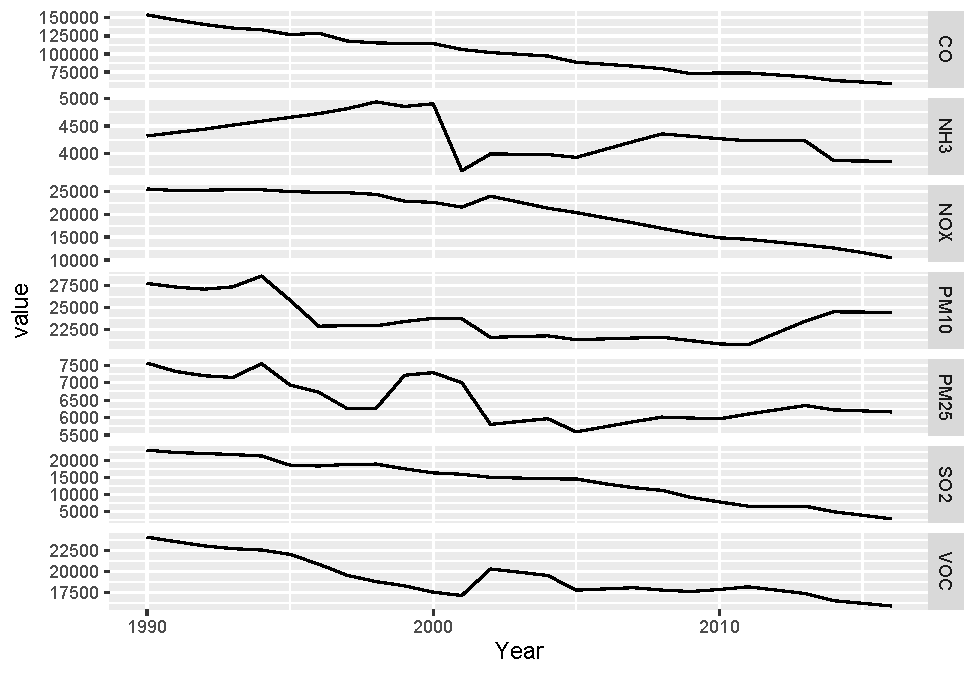
\includegraphics[width=0.75\linewidth]{EnvDataScience_files/figure-latex/USairpollution-1} 

}

\caption{Facet graph of air pollutants in the US, 1990-2016}\label{fig:USairpollution}
\end{figure}

\subsection{Flux tower data}\label{flux-tower-data}

While the above graphic comes from summary data, and it's certainly not
big data, when we're collecting data using an electronic data logger, we
can develop quite big datasets. Even data already summarized from
sub-second intervals to half hour values can be pretty voluminous so it
will be useful to be able to abstract the signal more clearly using
further grouped summaries.

We'll look at this data set in more depth in the time series chapter,
but here's a quick introduction. To look at micrometeorological changes
related to phenological changes in vegetation from seasonal hydrologic
changes from snowmelt through summer drying, we captured an array of
variables at a flux tower in Loney Meadow in the South Yuba River
watershed of the northern Sierra during the 2016 season (Figure
\ref{fig:transLoneyFlux}).

\begin{figure}

{\centering 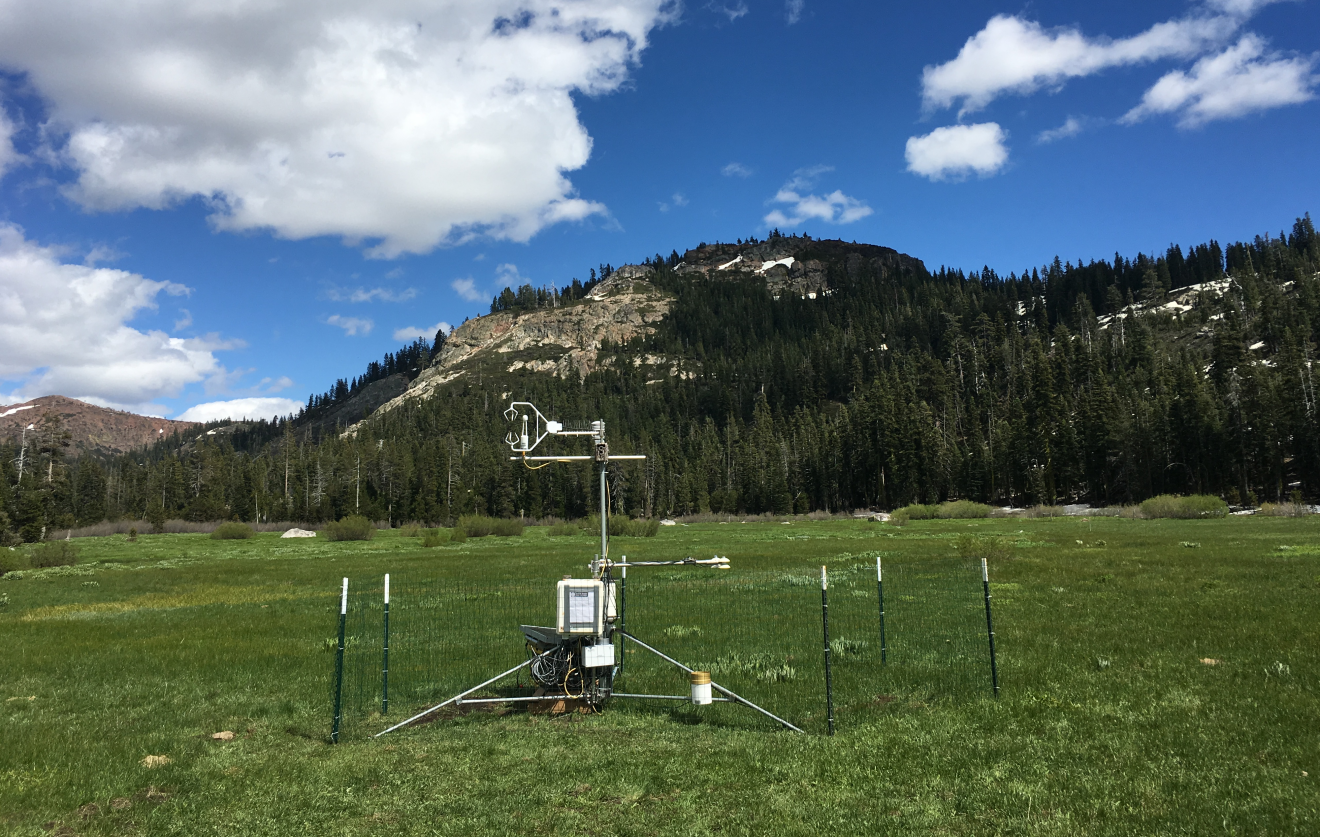
\includegraphics[width=0.75\linewidth]{img/LoneyFluxTowerWide} 

}

\caption{Flux tower installed at Loney Meadow, 2016. Photo credit: Darren Blackburn}\label{fig:transLoneyFlux}
\end{figure}

A spreadsheet of 30-minute summaries from 17 May to 6 September can be
found in the igisci extdata folder as
``meadows/LoneyMeadow\_30minCO2fluxes\_Geog604.xls'', and among other
parameters includes data on CO\textsubscript{2} flux, net radiation (Qnet), air
temperature (Tair), and relative humidity (RH). There's clearly a lot
more we can do with this data (see Blackburn et al. (\citeproc{ref-blackburn2021carbon}{2021})), but we'll
look at this selection of parameters to see how we can use a pivot to
create a multi-parameter graph.

First, we'll read in the data and simplify some of the variables. Since
the second row of data contains measurement units, we needed to wrangle
the data a bit to capture the variable names then add those back after
removing the first two rows:

\begin{Shaded}
\begin{Highlighting}[]
\FunctionTok{library}\NormalTok{(readxl); }\FunctionTok{library}\NormalTok{(tidyverse); }\FunctionTok{library}\NormalTok{(lubridate); }\FunctionTok{library}\NormalTok{(igisci)}
\NormalTok{vnames }\OtherTok{\textless{}{-}} \FunctionTok{read\_xls}\NormalTok{(}\FunctionTok{ex}\NormalTok{(}\StringTok{"meadows/LoneyMeadow\_30minCO2fluxes\_Geog604.xls"}\NormalTok{),}
                   \AttributeTok{n\_max=}\DecValTok{0}\NormalTok{) }\SpecialCharTok{|\textgreater{}} \FunctionTok{names}\NormalTok{()}
\NormalTok{vunits }\OtherTok{\textless{}{-}} \FunctionTok{read\_xls}\NormalTok{(}\FunctionTok{ex}\NormalTok{(}\StringTok{"meadows/LoneyMeadow\_30minCO2fluxes\_Geog604.xls"}\NormalTok{), }
                   \AttributeTok{n\_max=}\DecValTok{0}\NormalTok{, }\AttributeTok{skip=}\DecValTok{1}\NormalTok{) }\SpecialCharTok{|\textgreater{}} \FunctionTok{names}\NormalTok{()}
\NormalTok{Loney }\OtherTok{\textless{}{-}} \FunctionTok{read\_xls}\NormalTok{(}\FunctionTok{ex}\NormalTok{(}\StringTok{"meadows/LoneyMeadow\_30minCO2fluxes\_Geog604.xls"}\NormalTok{), }
                  \AttributeTok{skip=}\DecValTok{2}\NormalTok{, }\AttributeTok{col\_names=}\NormalTok{vnames) }\SpecialCharTok{|\textgreater{}}
         \FunctionTok{rename}\NormalTok{(}\AttributeTok{YDay =} \StringTok{\textasciigrave{}}\AttributeTok{Day of Year}\StringTok{\textasciigrave{}}\NormalTok{, }\AttributeTok{CO2flux =} \StringTok{\textasciigrave{}}\AttributeTok{CO2 Flux}\StringTok{\textasciigrave{}}\NormalTok{)}
\end{Highlighting}
\end{Shaded}

The time unit we'll want to use for time series is going to be days, and
we can also then look at the data over time, and a group\_by
summarization by days will give us a generalized picture of changes over
the collection period reflecting phenological changes from first
exposure after snowmelt through the maximum growth period and through
the major senescence period of late summer. We'll create the data to
graph by using a group\_by summarize to create a daily picture of a
selection of four micrometeorological parameters:

\begin{Shaded}
\begin{Highlighting}[]
\NormalTok{LoneyDaily }\OtherTok{\textless{}{-}}\NormalTok{ Loney }\SpecialCharTok{|\textgreater{}}
  \FunctionTok{group\_by}\NormalTok{(YDay) }\SpecialCharTok{|\textgreater{}}
  \FunctionTok{summarize}\NormalTok{(}\AttributeTok{CO2flux =} \FunctionTok{mean}\NormalTok{(CO2flux),}
            \AttributeTok{Qnet =} \FunctionTok{mean}\NormalTok{(Qnet),}
            \AttributeTok{Tair =} \FunctionTok{mean}\NormalTok{(Tair),}
            \AttributeTok{RH =} \FunctionTok{mean}\NormalTok{(RH))}
\end{Highlighting}
\end{Shaded}

\begin{quote}
Note that YDay is essentially an integer variable. While
\texttt{typeof(Loney\$YDay)} will return \texttt{"double"}, there are only integer
numeric values, so they will work to define groups -- for summary
values for each given day. In fact, there's no requirement that groups
defined by a numeric value be an integer; there just need to be
multiple instances of that value. In the time series chapter, we'll
group flux-tower micrometeorological values (like temperature) by
half-hour periods over the day (0, 0.5, 1.0, 1.5, \ldots, 23.5), with a
season of days providing values to summarize by those periods.
\end{quote}

Then from this daily data frame, we pivot\_longer to store all of the
parameter names in a \texttt{parameter} variable and all parameter values in a
\texttt{value} variable:

\begin{Shaded}
\begin{Highlighting}[]
\NormalTok{LoneyDailyLong }\OtherTok{\textless{}{-}}\NormalTok{ LoneyDaily }\SpecialCharTok{|\textgreater{}}
  \FunctionTok{pivot\_longer}\NormalTok{(}\AttributeTok{cols =}\NormalTok{ CO2flux}\SpecialCharTok{:}\NormalTok{RH,}
               \AttributeTok{names\_to=}\StringTok{"parameter"}\NormalTok{,}
               \AttributeTok{values\_to=}\StringTok{"value"}\NormalTok{) }\SpecialCharTok{|\textgreater{}}
  \FunctionTok{filter}\NormalTok{(parameter }\SpecialCharTok{\%in\%} \FunctionTok{c}\NormalTok{(}\StringTok{"CO2flux"}\NormalTok{, }\StringTok{"Qnet"}\NormalTok{, }\StringTok{"Tair"}\NormalTok{, }\StringTok{"RH"}\NormalTok{))}
\end{Highlighting}
\end{Shaded}

Now we have what we need to create a multi-parameter graph using
facet\_grid -- note the scales = ``free\_y'' setting to allow each
variable's y axis to correspond to its value range (Figure
\ref{fig:transFacet}).

\begin{Shaded}
\begin{Highlighting}[]
\NormalTok{p }\OtherTok{\textless{}{-}} \FunctionTok{ggplot}\NormalTok{(}\AttributeTok{data =}\NormalTok{ LoneyDailyLong, }\FunctionTok{aes}\NormalTok{(}\AttributeTok{x=}\NormalTok{YDay, }\AttributeTok{y=}\NormalTok{value)) }\SpecialCharTok{+} 
  \FunctionTok{geom\_line}\NormalTok{()}
\NormalTok{p }\SpecialCharTok{+} \FunctionTok{facet\_grid}\NormalTok{(parameter }\SpecialCharTok{\textasciitilde{}}\NormalTok{ ., }\AttributeTok{scales =} \StringTok{"free\_y"}\NormalTok{)}
\end{Highlighting}
\end{Shaded}

\begin{figure}

{\centering 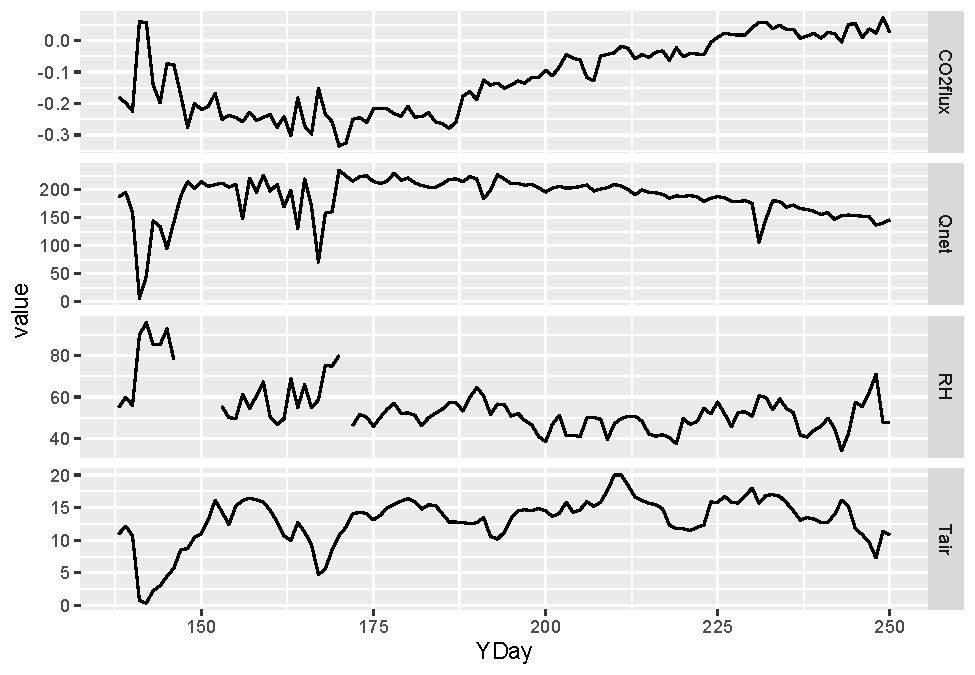
\includegraphics[width=0.75\linewidth]{EnvDataScience_files/figure-latex/transFacet-1} 

}

\caption{free-y facet graph supported by pivot (note the y axis scaling varies among variables)}\label{fig:transFacet}
\end{figure}

The need to create a similar graph from soil CO\textsubscript{2} data inspired me
years ago to learn how to program Excel. It was otherwise impossible to
get Excel to make all the x scales the same, so I learned how to force
it with code\ldots{}

\pagebreak

\section{Exercise: Transformation}\label{exercise-transformation}

\emph{by Josh von Nonn (2021)}

The impetus behind this exercise came from the movie \emph{Dark Waters}
(\url{https://www.youtube.com/watch?v=RvAOuhyunhY}), inspired by a true
story of negligent chemical waste disposal by Dupont.

First create a new RStudio project, named \texttt{GAMA} and save this .Rmd file
there, and create a folder \texttt{GAMA\_water\_data} in the project folder; the
path to the data can then be specifierd as
\texttt{"GAMA\_water\_data/gama\_pfas\_statewide\_v2.txt"} assuming that the latter
name matches what is unzipped from your download. Change to match the
actual name if it differs.

Then download from the California Water Boards, GAMA groundwater
website: \url{https://gamagroundwater.waterboards.ca.gov/gama/datadownload}

Then select ``Statewide Downloads'' then ``Statewide PFOS Data'' and extract
the zip file into the \texttt{GAMA\_water\_data} folder. This is a large txt file
so if you open it with notepad it may take some time to load. Notice
that this is a tab-delimited file, so is best read with \texttt{read.delim()} which defaults to tabs.

\textbf{Note} that this data structure is similar to what was discussed in
the introductory chapter in how you should use RStudio projects to
organize your data, allowing \emph{relative paths} to your data, such as
``GAMA\_water\_data/gama\_pfas\_statewide\_v2.txt'', which will work wherever
you copy your project folder. An absolute path to somewhere on your
computer in contrast won't work for anyone else trying to run your code;
absolute paths should only be used for servers that other users have
access to and URLs on the web.

Required packages:

\begin{Shaded}
\begin{Highlighting}[]
\FunctionTok{library}\NormalTok{(tidyverse)}
\FunctionTok{library}\NormalTok{(lubridate)}
\end{Highlighting}
\end{Shaded}

\begin{enumerate}
\def\labelenumi{\arabic{enumi}.}
\tightlist
\item
  Read in the downloaded file \texttt{"gama\_pfas\_statewide\_v2.txt"} and call
  it \texttt{cal\_pfas} and have a look at the data set. You can select it
  from the Environment pane or use \texttt{view(cal\_pfas)}.
\end{enumerate}

\begin{Shaded}
\begin{Highlighting}[]
\FunctionTok{library}\NormalTok{(tidyverse)}
\NormalTok{cal\_pfas }\OtherTok{\textless{}{-}} \FunctionTok{read.delim}\NormalTok{(}\StringTok{"GAMA\_water\_data}\SpecialCharTok{\textbackslash{}\textbackslash{}}\StringTok{gama\_pfas\_statewide\_v2.txt"}\NormalTok{)}
\end{Highlighting}
\end{Shaded}

\begin{enumerate}
\def\labelenumi{\arabic{enumi}.}
\setcounter{enumi}{1}
\item
  Before we clean up this data, let's preserve the locations of all
  the wells. Create a new data frame, \texttt{cal\_pfas\_loc}, retaining the
  well id and geographic coordinate variables (see 3.4.1) from the
  fields starting with \texttt{GM}, and remove all the duplicate wells (see
  3.3). (Hint: use \texttt{distinct()})
\item
  Now to trim down the data. Create a new data frame, \texttt{cal\_pfas\_trim};
  add a new \texttt{DATE} variable using the associated function (see 3.6) to
  read this from the GM sample collection date. Also from the GM
  fields, retain the date variable you just created, plus well id,
  chemical VVL, and the numerical result variables, and finally sort
  (see 3.4.7) by the well id.
\end{enumerate}

The resulting data frame should have the following structure:

\begin{enumerate}
\def\labelenumi{\arabic{enumi}.}
\setcounter{enumi}{3}
\tightlist
\item
  Use the method in 5.4.2 to create new columns from the chemical
  names and values from the result column and store the new data frame
  as \texttt{cal\_pfas\_wide}.\\
  \strut \\
  Notice the warnings. While we get a lot of warnings in R that are
  safely ignored (after you're used to those that are), we need to
  watch out for things that are going to give us results we don't
  want. Some of the wells have multiple samples on the same day so
  they will be put into a list (see this in the Environment tab). So
  we'll want to derive average values for those, so rerun the pivot
  but include the argument \texttt{values\_fn\ =\ mean}. This will return only
  the average of all the samples.\\
  \strut \\
  Once the pivot is working correctly, keep the variables
  \texttt{GM\_WELL\_ID},\texttt{DATE},\texttt{PFOS},\texttt{PFOA} and create a new one, \texttt{SUMPFS},
  that is the sum of \texttt{PFOS} and \texttt{PFOA}. See 3.4.1.
\end{enumerate}

\begin{quote}
The US EPA has established a lifetime Health Advisory Level (HAL) for
PFOA and PFOS of 70 ng/L. When both PFOA and PFOS are found in
drinking water, the combined concentrations of PFOA and PFOS should be
compared with the 70 ng/L HAL. From the GROUNDWATER INFORMATION SHEET
for PFOA
(website:\url{https://www.waterboards.ca.gov/water_issues/programs/gama/factsheets.html})
\end{quote}

\begin{enumerate}
\def\labelenumi{\arabic{enumi}.}
\setcounter{enumi}{4}
\item
  For the sake of creating an interesting time series plot, let's take
  the data frame you just created, filter data for wells that have a
  \texttt{SUMPFS} greater than 70 and that have more than 10 sampling dates
  (see 3.4.6; how many well ids do you have?). Start by creating a new
  data frame- \texttt{cal\_pfas\_index} from the pivoted data frame. Hint: one
  way to do this is to first filter, then count, then filter for a
  sufficient count. See 3.4.2 and 3.4.6. The resulting data frame
  downloaded in 2021 had 11 observations and 2 variables.
\item
  Create a new data frame, \texttt{cal\_pfas\_max} to locate the well with the
  most sampling dates (n). See 3.4.3, where we found the most massive
  female penguins, for a relevant method.
\item
  Now let's pull all the data on that well by joining the max indexed
  well with \texttt{cal\_pfas\_wide}, remove \texttt{n} (3.4.1), and call the new data
  frame \texttt{cal\_pfas\_join}.
\item
  Create a new data frame, \texttt{cal\_pfs\_long} and \texttt{pivot\_longer} the
  \texttt{cal\_pfs\_join} data, creating new columns: \texttt{"Chemical"} and \texttt{"ngl"}.
\item
  Plot the well using the wide data from \texttt{cal\_pfs\_join} , to create
  the graph shown here (see 4.4.3.1 and 4.7), plotting the three
  variables (\texttt{PFOS,PFOA,SUMPFS}) with different colored lines of your
  choice. Add a horizontal reference line
  (\texttt{geom\_hline(yintercept\ =\ 70)}) for the HAL limit at 70. Note that
  the axis labels have been clarified (see 4.7).
\end{enumerate}

\begin{center}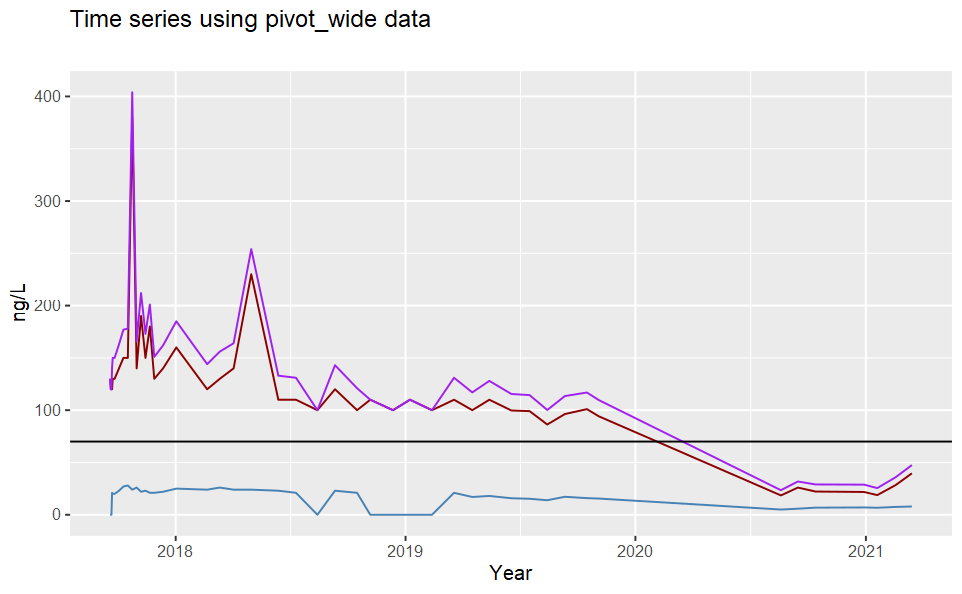
\includegraphics[width=0.75\linewidth]{img/transform_ex9} \end{center}

\begin{enumerate}
\def\labelenumi{\arabic{enumi}.}
\setcounter{enumi}{9}
\tightlist
\item
  Plot the well using the long data from \texttt{cal\_pfs\_long} using DATE on
  the x axis and \texttt{ngl} on the y axis. Distinguish the chemicals by
  setting the line color to \texttt{Chemical} in the aesthetics. As before,
  add the horizontal reference at 70 and improve the axis labels, but
  also tweak where the legend goes (see 4.7).
\end{enumerate}

\begin{figure}

{\centering 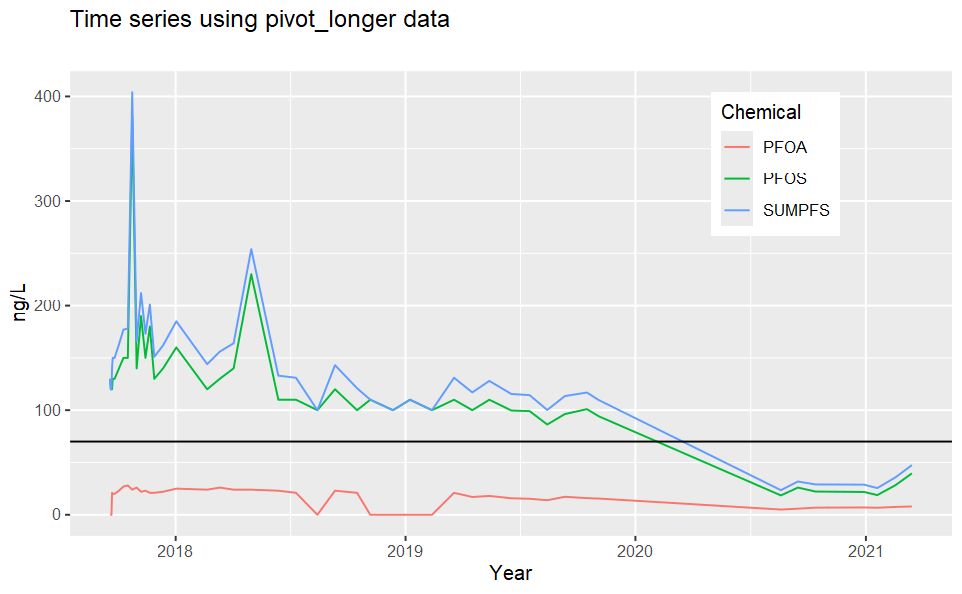
\includegraphics[width=0.5\linewidth]{img/transform_ex10} 

}

\caption{Goal}\label{fig:transGoal10}
\end{figure}

\part{Spatial}\label{part-spatial}

\chapter{Spatial Data and Maps}\label{spatial}

\begin{center}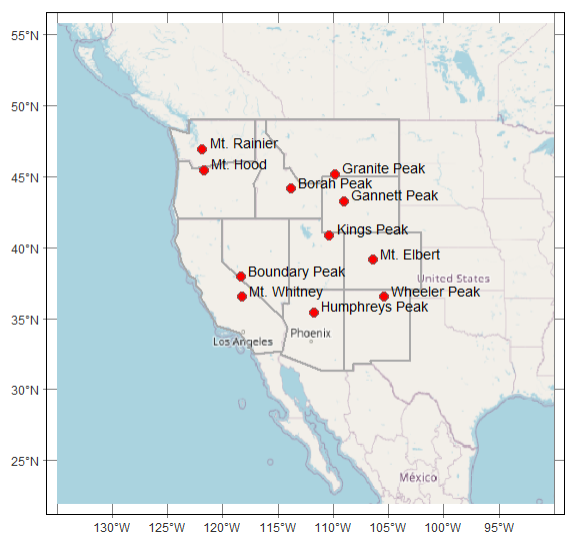
\includegraphics[width=0.75\linewidth]{img/goal_SpatialDataMaps10} \end{center}

The Spatial section of this book adds the \index{spatial dimension}spatial dimension and \index{geographic data science}\emph{geographic} data science. Most environmental systems are significantly affected by location, so the geographic perspective is highly informative. In this chapter, we'll explore the basics of

\begin{itemize}
\tightlist
\item
  building and using feature-based (vector) data using the \texttt{sf} (simple features) package
\item
  raster data using the \texttt{terra} package
\item
  some common mapping methods in \texttt{plot} and \texttt{ggplot2}
\end{itemize}

Especially for the feature data, which is built on a database model (with geometry as one variable), the tools we've been learning in \texttt{dplyr} and \texttt{tidyr} will also be useful to working with attributes.

\emph{Caveat}: Spatial data and analysis is very useful for environmental data analysis, and we'll only scratch the surface. Readers are encouraged to explore other resources on this important topic, such as:

\begin{itemize}
\tightlist
\item
  \emph{Geocomputation with R} at \url{https://geocompr.robinlovelace.net/}
\item
  \emph{Simple Features for R} at \url{https://r-spatial.github.io/sf/}
\item
  \emph{Spatial Data Science with R} at \url{https://rspatial.org}
\end{itemize}

\section{Spatial Data}\label{spatial-data}

\index{spatial data}Spatial data is data using a Cartesian coordinate system with x, y, z, and maybe more dimensions. Geospatial data is spatial data that we can map on our planet and relate to other geospatial data based on geographic coordinate systems (GCS) of longitude and latitude or known projections to planar coordinates like Mercator, Albers, or many others. You can also use local coordinate systems with the methods we'll learn, to describe geometric objects or a local coordinate system to ``map out'' an archaeological dig or describe the movement of ants on an anthill, but we'll primarily use geospatial data.

To work with spatial data requires extending R to deal with it using packages. Many have been developed, but the field is starting to mature using international open GIS standards.

\textbf{\texttt{sp}} (until recently, the dominant library of spatial tools)

\begin{itemize}
\tightlist
\item
  Includes functions for working with spatial data
\item
  Includes \texttt{spplot} to create maps
\item
  Also needs \texttt{rgdal} package for \texttt{readOGR} -- reads spatial data frames
\item
  Earliest archived version on CRAN is 0.7-3, 2005-04-28, with 1.0 released 2012-09-30. Authors: Edzer Pebesma and Roger Bivand
\end{itemize}

\textbf{\texttt{sf}} (Simple Features)\index{sf simple features}

\begin{itemize}
\tightlist
\item
  Feature-based (vector) methods
\item
  ISO 19125 standard for GIS geometries
\item
  Also has functions for working with spatial data, but clearer to use
\item
  Doesn't need many additional packages, though you may still need \texttt{rgdal} installed for some tools you want to use
\item
  Replacing \texttt{sp} and \texttt{spplot} though you'll still find them in code
\item
  Works with ggplot2 and tmap for nice looking maps
\item
  Cheat sheet and other information at \url{https://r-spatial.github.io/sf/}
\item
  Earliest CRAN archive is 0.2 on 2016-10-26, 1.0 not until 2021-06-29
\item
  Author: Edzer Pebesma
\end{itemize}

\textbf{\texttt{raster}}\index{raster package}

\begin{itemize}
\tightlist
\item
  The established raster package for R, with version 1.0 from 2010-03-20, Author: Robert J. Hijmans (Professor of Environmental Science and Policy at UC Davis)
\item
  Depends on \texttt{sp}
\item
  CRAN: ``Reading, writing, manipulating, analyzing and modeling of spatial data. The package implements basic and high-level functions for raster data and for vector data operations such as intersections. See the manual and tutorials on \url{https://rspatial.org/} to get started.''
\end{itemize}

\textbf{\texttt{terra}}\index{terra package}

\begin{itemize}
\tightlist
\item
  Intended to eventually replace \texttt{raster}, by the same author (Hijmans), current version 1.6-7 2022-08-07; does not depend on \texttt{sp}, but includes Bivand and Pebesma as contributors
\item
  CRAN: ``Methods for spatial data analysis with raster and vector data. Raster methods allow for low-level data manipulation as well as high-level global, local, zonal, and focal computation. The predict and interpolate methods facilitate the use of regression type (interpolation, machine learning) models for spatial prediction, including with satellite remote sensing data. Processing of very large files is supported. See the manual and tutorials on \url{https://rspatial.org/terra/} to get started.''
\end{itemize}

\subsection{Simple geometry building in sf}\label{simple-geometry-building-in-sf}

\index{simple geometry building in sf}Simple Features (\texttt{sf}) includes a set of simple geometry building tools that use matrices or lists of matrices of XYZ (or just XY) coordinates (or lists of lists for multipolygon) as input, and each basic geometry type having single and multiple versions (Table \ref{tab:mapsSimpleGeometrySF}). Note that sf functions have the pattern \texttt{st\_*} (st means ``space and time'').

\begin{table}
\centering
\caption{\label{tab:mapsSimpleGeometrySF}Some common sf functions for building geometries from coordinates}
\centering
\begin{tabular}[t]{ll}
\toprule
sf function & input\\
\midrule
st\_point() & numeric vector of length 2, 3, or 4, represent a single point\\
st\_multipoint() & numeric matrix with points in rows\\
st\_linestring() & numeric matrix with points in rows\\
st\_multilinestring() & list of numeric matrices with points in rows\\
st\_polygon() & list of numeric matrices with points in rows\\
\addlinespace
st\_multipolygon() & list of lists with numeric matrices\\
\bottomrule
\end{tabular}
\end{table}

\begin{Shaded}
\begin{Highlighting}[]
\FunctionTok{library}\NormalTok{(tidyverse)}
\FunctionTok{library}\NormalTok{(sf)}
\FunctionTok{library}\NormalTok{(igisci)}
\end{Highlighting}
\end{Shaded}

\subsubsection{Building simple sf geometries}\label{building-simple-sf-geometries}

\index{geometries, sf}We'll build some simple geometries and plot them, just to illustrate the types of geometries. Try the following code.

\begin{Shaded}
\begin{Highlighting}[]
\FunctionTok{library}\NormalTok{(sf); }\FunctionTok{library}\NormalTok{(tidyverse)}
\NormalTok{eyes }\OtherTok{\textless{}{-}} \FunctionTok{st\_multipoint}\NormalTok{(}\FunctionTok{rbind}\NormalTok{(}\FunctionTok{c}\NormalTok{(}\DecValTok{1}\NormalTok{,}\DecValTok{5}\NormalTok{), }\FunctionTok{c}\NormalTok{(}\DecValTok{3}\NormalTok{,}\DecValTok{5}\NormalTok{)))}
\NormalTok{nose }\OtherTok{\textless{}{-}} \FunctionTok{st\_point}\NormalTok{(}\FunctionTok{c}\NormalTok{(}\DecValTok{2}\NormalTok{,}\DecValTok{4}\NormalTok{))}
\NormalTok{mouth }\OtherTok{\textless{}{-}} \FunctionTok{st\_linestring}\NormalTok{(}\FunctionTok{rbind}\NormalTok{(}\FunctionTok{c}\NormalTok{(}\DecValTok{1}\NormalTok{,}\DecValTok{3}\NormalTok{),}\FunctionTok{c}\NormalTok{(}\DecValTok{3}\NormalTok{, }\DecValTok{3}\NormalTok{)))}
\NormalTok{border }\OtherTok{\textless{}{-}} \FunctionTok{st\_polygon}\NormalTok{(}\FunctionTok{list}\NormalTok{(}\FunctionTok{rbind}\NormalTok{(}\FunctionTok{c}\NormalTok{(}\DecValTok{0}\NormalTok{,}\DecValTok{5}\NormalTok{), }\FunctionTok{c}\NormalTok{(}\DecValTok{1}\NormalTok{,}\DecValTok{2}\NormalTok{), }\FunctionTok{c}\NormalTok{(}\DecValTok{2}\NormalTok{,}\DecValTok{1}\NormalTok{), }\FunctionTok{c}\NormalTok{(}\DecValTok{3}\NormalTok{,}\DecValTok{2}\NormalTok{), }
                              \FunctionTok{c}\NormalTok{(}\DecValTok{4}\NormalTok{,}\DecValTok{5}\NormalTok{), }\FunctionTok{c}\NormalTok{(}\DecValTok{3}\NormalTok{,}\DecValTok{7}\NormalTok{), }\FunctionTok{c}\NormalTok{(}\DecValTok{1}\NormalTok{,}\DecValTok{7}\NormalTok{), }\FunctionTok{c}\NormalTok{(}\DecValTok{0}\NormalTok{,}\DecValTok{5}\NormalTok{))))}
\FunctionTok{plot}\NormalTok{(}\FunctionTok{st\_sfc}\NormalTok{(eyes, nose, mouth, border))}
\end{Highlighting}
\end{Shaded}

\subsubsection{\texorpdfstring{Building geospatial points as sf columns (\texttt{sfc})}{Building geospatial points as sf columns (sfc)}}\label{maps}

\index{sfc sf columns}The face-building example above is really intended for helping to understand the concept and isn't really how we'd typically build data. For one thing, it doesn't have a real coordinate system that can be reprojected into locations anywhere on the planet. And while it allows it, building an sfc from a mixture of geometry types (poin, linestring, and polygon) isn't recommended for geospatial data.

See Geocomputation with R at \url{https://geocompr.robinlovelace.net/} or \url{https://r-spatial.github.io/sf/} for more details, but when building spatial data from scratch, we would need to follow this by building a simple feature geometry list column from the collection with \texttt{st\_sfc()}. We'll look at this using real geographic coordinates, building a generalized map of California and Nevada boundaries (and then later in the exercises, you'll expand this to a map of the west.) We'll use a shortcut to the coordinate referencing system (crs) by using a short numeric EPSG code (\emph{EPSG Geodetic Parameter Dataset} (\citeproc{ref-epsg}{n.d.})), 4326, for the common geographic coordinate system (GCS) of latitude and longitude.

\begin{Shaded}
\begin{Highlighting}[]
\FunctionTok{library}\NormalTok{(sf)}
\NormalTok{CA\_matrix }\OtherTok{\textless{}{-}} \FunctionTok{rbind}\NormalTok{(}\FunctionTok{c}\NormalTok{(}\SpecialCharTok{{-}}\DecValTok{124}\NormalTok{,}\DecValTok{42}\NormalTok{),}\FunctionTok{c}\NormalTok{(}\SpecialCharTok{{-}}\DecValTok{120}\NormalTok{,}\DecValTok{42}\NormalTok{),}\FunctionTok{c}\NormalTok{(}\SpecialCharTok{{-}}\DecValTok{120}\NormalTok{,}\DecValTok{39}\NormalTok{),}\FunctionTok{c}\NormalTok{(}\SpecialCharTok{{-}}\FloatTok{114.5}\NormalTok{,}\DecValTok{35}\NormalTok{),}
  \FunctionTok{c}\NormalTok{(}\SpecialCharTok{{-}}\FloatTok{114.1}\NormalTok{,}\FloatTok{34.3}\NormalTok{),}\FunctionTok{c}\NormalTok{(}\SpecialCharTok{{-}}\FloatTok{114.7}\NormalTok{,}\FloatTok{33.4}\NormalTok{),}\FunctionTok{c}\NormalTok{(}\SpecialCharTok{{-}}\FloatTok{114.5}\NormalTok{,}\DecValTok{33}\NormalTok{),}
  \FunctionTok{c}\NormalTok{(}\SpecialCharTok{{-}}\FloatTok{114.6}\NormalTok{,}\FloatTok{32.7}\NormalTok{),}\FunctionTok{c}\NormalTok{(}\SpecialCharTok{{-}}\DecValTok{117}\NormalTok{,}\FloatTok{32.5}\NormalTok{),}\FunctionTok{c}\NormalTok{(}\SpecialCharTok{{-}}\FloatTok{118.5}\NormalTok{,}\DecValTok{34}\NormalTok{),}\FunctionTok{c}\NormalTok{(}\SpecialCharTok{{-}}\FloatTok{120.5}\NormalTok{,}\FloatTok{34.5}\NormalTok{),}
  \FunctionTok{c}\NormalTok{(}\SpecialCharTok{{-}}\DecValTok{122}\NormalTok{,}\FloatTok{36.5}\NormalTok{),}\FunctionTok{c}\NormalTok{(}\SpecialCharTok{{-}}\FloatTok{121.8}\NormalTok{,}\FloatTok{36.8}\NormalTok{),}\FunctionTok{c}\NormalTok{(}\SpecialCharTok{{-}}\DecValTok{122}\NormalTok{,}\DecValTok{37}\NormalTok{),}\FunctionTok{c}\NormalTok{(}\SpecialCharTok{{-}}\FloatTok{122.4}\NormalTok{,}\FloatTok{37.3}\NormalTok{),}\FunctionTok{c}\NormalTok{(}\SpecialCharTok{{-}}\FloatTok{122.5}\NormalTok{,}\FloatTok{37.8}\NormalTok{),}
  \FunctionTok{c}\NormalTok{(}\SpecialCharTok{{-}}\DecValTok{123}\NormalTok{,}\DecValTok{38}\NormalTok{),}\FunctionTok{c}\NormalTok{(}\SpecialCharTok{{-}}\FloatTok{123.7}\NormalTok{,}\DecValTok{39}\NormalTok{),}\FunctionTok{c}\NormalTok{(}\SpecialCharTok{{-}}\DecValTok{124}\NormalTok{,}\DecValTok{40}\NormalTok{),}\FunctionTok{c}\NormalTok{(}\SpecialCharTok{{-}}\FloatTok{124.4}\NormalTok{,}\FloatTok{40.5}\NormalTok{),}\FunctionTok{c}\NormalTok{(}\SpecialCharTok{{-}}\DecValTok{124}\NormalTok{,}\DecValTok{41}\NormalTok{),}\FunctionTok{c}\NormalTok{(}\SpecialCharTok{{-}}\DecValTok{124}\NormalTok{,}\DecValTok{42}\NormalTok{))}
\NormalTok{NV\_matrix }\OtherTok{\textless{}{-}} \FunctionTok{rbind}\NormalTok{(}\FunctionTok{c}\NormalTok{(}\SpecialCharTok{{-}}\DecValTok{120}\NormalTok{,}\DecValTok{42}\NormalTok{),}\FunctionTok{c}\NormalTok{(}\SpecialCharTok{{-}}\DecValTok{114}\NormalTok{,}\DecValTok{42}\NormalTok{),}\FunctionTok{c}\NormalTok{(}\SpecialCharTok{{-}}\DecValTok{114}\NormalTok{,}\DecValTok{36}\NormalTok{),}\FunctionTok{c}\NormalTok{(}\SpecialCharTok{{-}}\FloatTok{114.2}\NormalTok{,}\DecValTok{36}\NormalTok{),}
  \FunctionTok{c}\NormalTok{(}\SpecialCharTok{{-}}\FloatTok{114.4}\NormalTok{,}\FloatTok{36.2}\NormalTok{),}\FunctionTok{c}\NormalTok{(}\SpecialCharTok{{-}}\FloatTok{114.7}\NormalTok{,}\DecValTok{36}\NormalTok{),}\FunctionTok{c}\NormalTok{(}\SpecialCharTok{{-}}\FloatTok{114.5}\NormalTok{,}\DecValTok{35}\NormalTok{),}\FunctionTok{c}\NormalTok{(}\SpecialCharTok{{-}}\DecValTok{120}\NormalTok{,}\DecValTok{39}\NormalTok{),}\FunctionTok{c}\NormalTok{(}\SpecialCharTok{{-}}\DecValTok{120}\NormalTok{,}\DecValTok{42}\NormalTok{))}
\NormalTok{CA\_list }\OtherTok{\textless{}{-}} \FunctionTok{list}\NormalTok{(CA\_matrix);       NV\_list }\OtherTok{\textless{}{-}} \FunctionTok{list}\NormalTok{(NV\_matrix)}
\NormalTok{CA\_poly }\OtherTok{\textless{}{-}} \FunctionTok{st\_polygon}\NormalTok{(CA\_list);   NV\_poly }\OtherTok{\textless{}{-}} \FunctionTok{st\_polygon}\NormalTok{(NV\_list)}
\NormalTok{sfc\_2states }\OtherTok{\textless{}{-}} \FunctionTok{st\_sfc}\NormalTok{(CA\_poly,NV\_poly,}\AttributeTok{crs=}\DecValTok{4326}\NormalTok{)  }\CommentTok{\# crs=4326 specifies GCS}
\FunctionTok{st\_geometry\_type}\NormalTok{(sfc\_2states)}
\end{Highlighting}
\end{Shaded}

\begin{verbatim}
## [1] POLYGON POLYGON
## 18 Levels: GEOMETRY POINT LINESTRING POLYGON MULTIPOINT ... TRIANGLE
\end{verbatim}

Now that we have simple feature columns for two state polygons, let's build a polyline of the Colorado River which forms part of the boundary of California and Nevada, so some of these vertices are copied from those.

\begin{Shaded}
\begin{Highlighting}[]
\NormalTok{CO\_river }\OtherTok{=} \FunctionTok{st\_sfc}\NormalTok{(}\FunctionTok{st\_linestring}\NormalTok{(}\FunctionTok{rbind}\NormalTok{(}\FunctionTok{c}\NormalTok{(}\SpecialCharTok{{-}}\DecValTok{114}\NormalTok{,}\DecValTok{36}\NormalTok{),}\FunctionTok{c}\NormalTok{(}\SpecialCharTok{{-}}\FloatTok{114.2}\NormalTok{,}\DecValTok{36}\NormalTok{),}\FunctionTok{c}\NormalTok{(}\SpecialCharTok{{-}}\FloatTok{114.4}\NormalTok{,}\FloatTok{36.2}\NormalTok{),}
    \FunctionTok{c}\NormalTok{(}\SpecialCharTok{{-}}\FloatTok{114.7}\NormalTok{,}\DecValTok{36}\NormalTok{),}\FunctionTok{c}\NormalTok{(}\SpecialCharTok{{-}}\FloatTok{114.5}\NormalTok{,}\DecValTok{35}\NormalTok{),}\FunctionTok{c}\NormalTok{(}\SpecialCharTok{{-}}\FloatTok{114.1}\NormalTok{,}\FloatTok{34.3}\NormalTok{),}\FunctionTok{c}\NormalTok{(}\SpecialCharTok{{-}}\FloatTok{114.7}\NormalTok{,}\FloatTok{33.4}\NormalTok{),}\FunctionTok{c}\NormalTok{(}\SpecialCharTok{{-}}\FloatTok{114.5}\NormalTok{,}\DecValTok{33}\NormalTok{),}
    \FunctionTok{c}\NormalTok{(}\SpecialCharTok{{-}}\FloatTok{114.6}\NormalTok{,}\FloatTok{32.7}\NormalTok{),}\FunctionTok{c}\NormalTok{(}\SpecialCharTok{{-}}\FloatTok{115.0}\NormalTok{,}\FloatTok{32.2}\NormalTok{),}\FunctionTok{c}\NormalTok{(}\SpecialCharTok{{-}}\FloatTok{114.8}\NormalTok{,}\FloatTok{31.8}\NormalTok{))),}\AttributeTok{crs=}\DecValTok{4326}\NormalTok{)}
\end{Highlighting}
\end{Shaded}

Then we'll use the \texttt{geom\_sf()} function in ggplot2 to create a map (Figure \ref{fig:mapsGG2}).

\begin{Shaded}
\begin{Highlighting}[]
\FunctionTok{library}\NormalTok{(tidyverse)}
\FunctionTok{ggplot}\NormalTok{() }\SpecialCharTok{+} \FunctionTok{geom\_sf}\NormalTok{(}\AttributeTok{data =}\NormalTok{ sfc\_2states) }\SpecialCharTok{+}
  \FunctionTok{geom\_sf}\NormalTok{(}\AttributeTok{data=}\NormalTok{CO\_river, }\AttributeTok{col=}\StringTok{"blue"}\NormalTok{)}
\end{Highlighting}
\end{Shaded}

\begin{figure}

{\centering 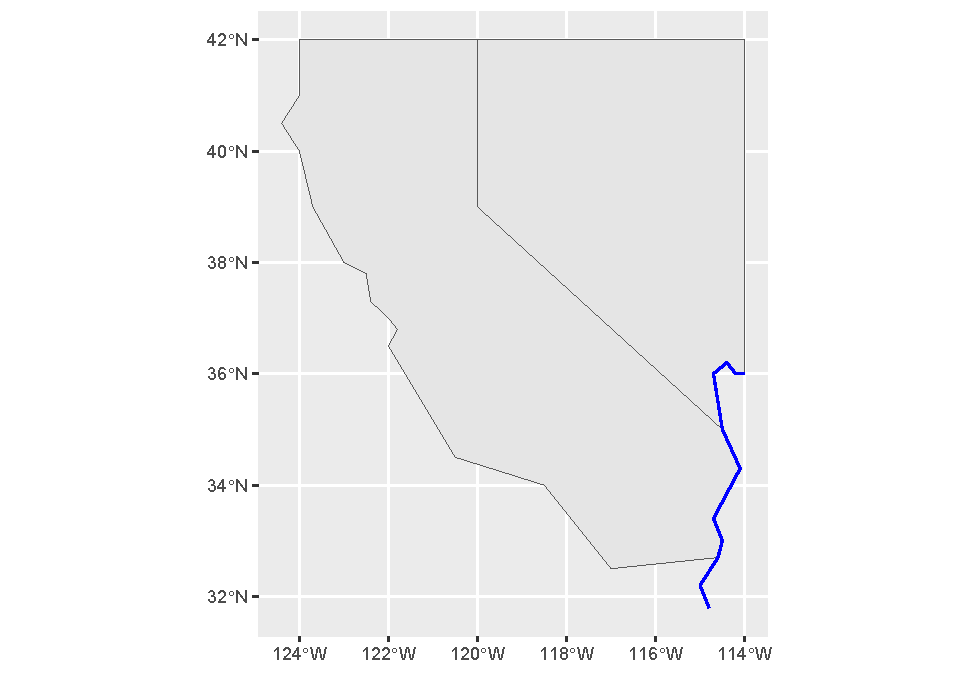
\includegraphics[width=0.75\linewidth]{EnvDataScience_files/figure-latex/mapsGG2-1} 

}

\caption{A simple ggplot2 map built from scratch with hard-coded data as simple feature columns}\label{fig:mapsGG2}
\end{figure}

\subsubsection{Building an sf class from sf columns.}\label{building-an-sf-class-from-sf-columns.}

\index{sf class}So far, we've built an \texttt{sfg} (sf geometry) and then a collection of matrices in an \texttt{sfc} (sf column), and we were even able to make a map of it. But to be truly useful, we'll want other attributes other than just where the feature is, so we'll build an \texttt{sf} that has attributes, and that can also be used like a data frame -- similar to a shapefile, since a data frame is like a database table \texttt{.dbf}. We'll build one with the \texttt{st\_sf()} function from attributes and geometry (Figure \ref{fig:mapsSFclass}).

\begin{quote}
Note that the first argument for \texttt{st\_sf} does not have a name. If you check the usage with \texttt{?st\_sf} you'll just see \texttt{...} for the first argument, and you simply are to provide ``column elements to be binded into an \texttt{sf} object''. In this case \texttt{attributes} is simply listed there; don't be tempted to be explicit and use something like \texttt{data=attributes}.
\end{quote}

\begin{Shaded}
\begin{Highlighting}[]
\NormalTok{attributes }\OtherTok{\textless{}{-}} \FunctionTok{bind\_rows}\NormalTok{(}\FunctionTok{c}\NormalTok{(}\AttributeTok{abb=}\StringTok{"CA"}\NormalTok{, }\AttributeTok{area=}\DecValTok{423970}\NormalTok{, }\AttributeTok{pop=}\FloatTok{39.56e6}\NormalTok{),}
                        \FunctionTok{c}\NormalTok{(}\AttributeTok{abb=}\StringTok{"NV"}\NormalTok{, }\AttributeTok{area=}\DecValTok{286382}\NormalTok{, }\AttributeTok{pop=}\FloatTok{3.03e6}\NormalTok{)) }\SpecialCharTok{\%\textgreater{}\%}
  \FunctionTok{mutate}\NormalTok{(}\AttributeTok{area=}\FunctionTok{as.numeric}\NormalTok{(area),}\AttributeTok{pop=}\FunctionTok{as.numeric}\NormalTok{(pop))}
\NormalTok{twostates }\OtherTok{\textless{}{-}} \FunctionTok{st\_sf}\NormalTok{(attributes, }\AttributeTok{geometry =}\NormalTok{ sfc\_2states)}
\NormalTok{river }\OtherTok{=} \FunctionTok{st\_sf}\NormalTok{(}\FunctionTok{tribble}\NormalTok{(}\SpecialCharTok{\textasciitilde{}}\NormalTok{name,}\StringTok{"Colorado River"}\NormalTok{), }\AttributeTok{geometry=}\NormalTok{CO\_river)}
\FunctionTok{ggplot}\NormalTok{(twostates) }\SpecialCharTok{+} \FunctionTok{geom\_sf}\NormalTok{() }\SpecialCharTok{+} \FunctionTok{geom\_sf\_text}\NormalTok{(}\FunctionTok{aes}\NormalTok{(}\AttributeTok{label =}\NormalTok{ abb)) }\SpecialCharTok{+}
  \FunctionTok{geom\_sf}\NormalTok{(}\AttributeTok{data=}\NormalTok{river, }\AttributeTok{col=}\StringTok{"blue"}\NormalTok{) }\SpecialCharTok{+}
  \FunctionTok{labs}\NormalTok{(}\AttributeTok{x=}\StringTok{""}\NormalTok{,}\AttributeTok{y=}\StringTok{""}\NormalTok{)}
\end{Highlighting}
\end{Shaded}

\begin{figure}

{\centering 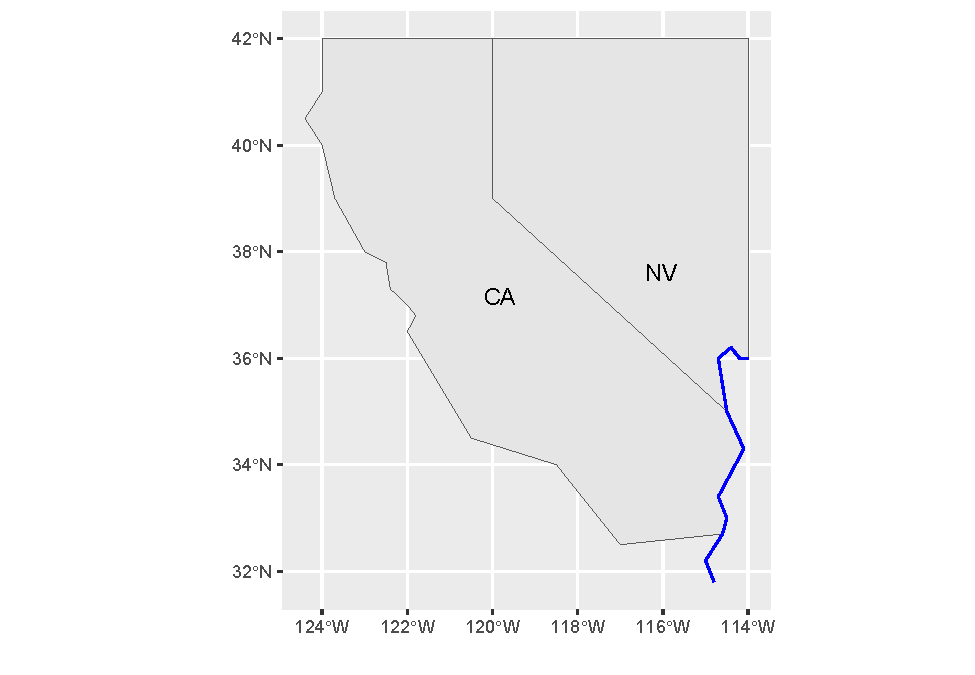
\includegraphics[width=0.75\linewidth]{EnvDataScience_files/figure-latex/mapsSFclass-1} 

}

\caption{Using an sf class to build a map in ggplot2, displaying an attribute}\label{fig:mapsSFclass}
\end{figure}

Or we could let the plot system try to figure out what to do with it. To help it out a bit, we can select just one variable, for which we need to use the \texttt{{[}{]}} accessor (Figure \ref{fig:mapsBaseR2states}). Try the \texttt{\$} accessor instead to see what you get, and consider why this might be.

\begin{Shaded}
\begin{Highlighting}[]
\FunctionTok{plot}\NormalTok{(twostates[}\StringTok{"abb"}\NormalTok{])}
\end{Highlighting}
\end{Shaded}

\begin{figure}

{\centering 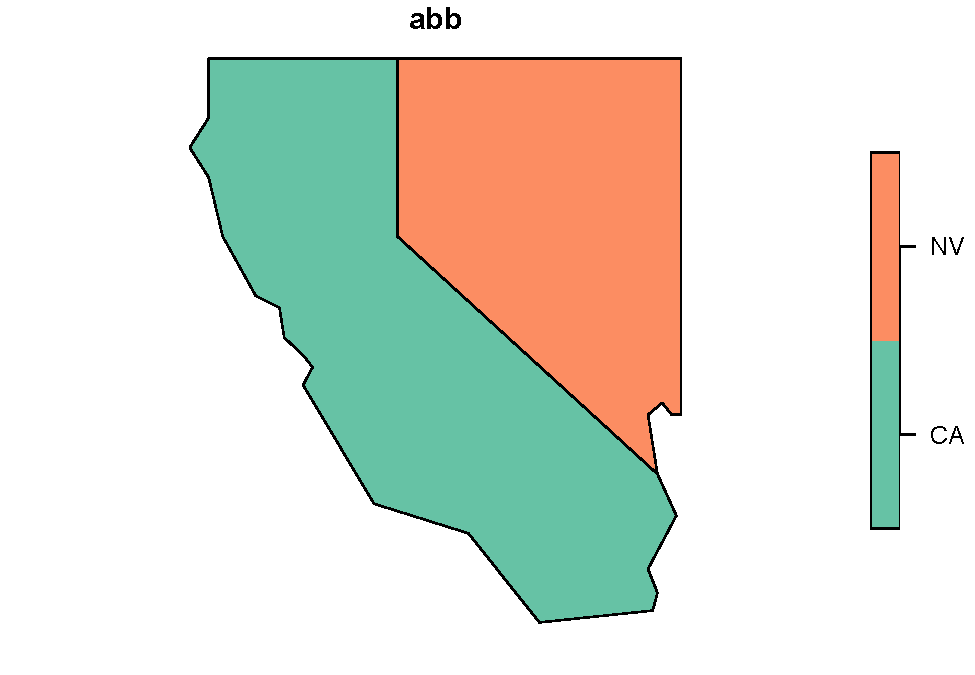
\includegraphics[width=0.75\linewidth]{EnvDataScience_files/figure-latex/mapsBaseR2states-1} 

}

\caption{Base R plot of one attribute from two states}\label{fig:mapsBaseR2states}
\end{figure}

\subsection{Building points from a data frame}\label{building-points-from-a-data-frame}

\index{points from a data frame}We're going to take a different approach with points, since if we're building them from scratch they commonly come in the form of a data frame with x and y columns, so the \texttt{st\_as\_sf} is much simpler than what we just did with \texttt{sfg} and \texttt{sfc} data.

The \texttt{sf::st\_as\_sf} function is useful for a lot of things, and follows the convention of R's many ``as'' functions: if it can understand the input as having ``space and time'' (st) data, it can convert it to an sf.

We'll start by creating a data frame representing 12 Sierra Nevada (and some adjacent) weather stations, with variables entered as vectors, including attributes. The order of vectors needs to be the same for all, where the first point has index 1, etc.

\begin{Shaded}
\begin{Highlighting}[]
\NormalTok{sta  }\OtherTok{\textless{}{-}} \FunctionTok{c}\NormalTok{(}\StringTok{"OROVILLE"}\NormalTok{,}\StringTok{"AUBURN"}\NormalTok{,}\StringTok{"PLACERVILLE"}\NormalTok{,}\StringTok{"COLFAX"}\NormalTok{,}\StringTok{"NEVADA CITY"}\NormalTok{,}\StringTok{"QUINCY"}\NormalTok{,}
          \StringTok{"YOSEMITE"}\NormalTok{,}\StringTok{"PORTOLA"}\NormalTok{,}\StringTok{"TRUCKEE"}\NormalTok{,}\StringTok{"BRIDGEPORT"}\NormalTok{,}\StringTok{"LEE VINING"}\NormalTok{,}\StringTok{"BODIE"}\NormalTok{)}
\NormalTok{lon }\OtherTok{\textless{}{-}} \FunctionTok{c}\NormalTok{(}\SpecialCharTok{{-}}\FloatTok{121.55}\NormalTok{,}\SpecialCharTok{{-}}\FloatTok{121.08}\NormalTok{,}\SpecialCharTok{{-}}\FloatTok{120.82}\NormalTok{,}\SpecialCharTok{{-}}\FloatTok{120.95}\NormalTok{,}\SpecialCharTok{{-}}\FloatTok{121.00}\NormalTok{,}\SpecialCharTok{{-}}\FloatTok{120.95}\NormalTok{,}
          \SpecialCharTok{{-}}\FloatTok{119.59}\NormalTok{,}\SpecialCharTok{{-}}\FloatTok{120.47}\NormalTok{,}\SpecialCharTok{{-}}\FloatTok{120.17}\NormalTok{,}\SpecialCharTok{{-}}\FloatTok{119.23}\NormalTok{,}\SpecialCharTok{{-}}\FloatTok{119.12}\NormalTok{,}\SpecialCharTok{{-}}\FloatTok{119.01}\NormalTok{)}
\NormalTok{lat }\OtherTok{\textless{}{-}}  \FunctionTok{c}\NormalTok{(}\FloatTok{39.52}\NormalTok{,}\FloatTok{38.91}\NormalTok{,}\FloatTok{38.70}\NormalTok{,}\FloatTok{39.09}\NormalTok{,}\FloatTok{39.25}\NormalTok{,}\FloatTok{39.94}\NormalTok{,}
          \FloatTok{37.75}\NormalTok{,}\FloatTok{39.81}\NormalTok{,}\FloatTok{39.33}\NormalTok{,}\FloatTok{38.26}\NormalTok{,}\FloatTok{37.96}\NormalTok{,}\FloatTok{38.21}\NormalTok{)}
\NormalTok{elev }\OtherTok{\textless{}{-}} \FunctionTok{c}\NormalTok{(}\DecValTok{52}\NormalTok{,}\DecValTok{394}\NormalTok{,}\DecValTok{564}\NormalTok{,}\DecValTok{725}\NormalTok{,}\DecValTok{848}\NormalTok{,}\DecValTok{1042}\NormalTok{,}
          \DecValTok{1225}\NormalTok{,}\DecValTok{1478}\NormalTok{,}\DecValTok{1775}\NormalTok{,}\DecValTok{1972}\NormalTok{,}\DecValTok{2072}\NormalTok{,}\DecValTok{2551}\NormalTok{)}
\NormalTok{tC }\OtherTok{\textless{}{-}} \FunctionTok{c}\NormalTok{(}\FloatTok{10.7}\NormalTok{,}\FloatTok{9.7}\NormalTok{,}\FloatTok{9.2}\NormalTok{,}\FloatTok{7.3}\NormalTok{,}\FloatTok{6.7}\NormalTok{,}\FloatTok{4.0}\NormalTok{,}
          \FloatTok{5.0}\NormalTok{,}\FloatTok{0.5}\NormalTok{,}\SpecialCharTok{{-}}\FloatTok{1.1}\NormalTok{,}\SpecialCharTok{{-}}\FloatTok{2.2}\NormalTok{,}\FloatTok{0.4}\NormalTok{,}\SpecialCharTok{{-}}\FloatTok{4.4}\NormalTok{)}
\NormalTok{prec }\OtherTok{\textless{}{-}} \FunctionTok{c}\NormalTok{(}\DecValTok{124}\NormalTok{,}\DecValTok{160}\NormalTok{,}\DecValTok{171}\NormalTok{,}\DecValTok{207}\NormalTok{,}\DecValTok{268}\NormalTok{,}\DecValTok{182}\NormalTok{,}
          \DecValTok{169}\NormalTok{,}\DecValTok{98}\NormalTok{,}\DecValTok{126}\NormalTok{,}\DecValTok{41}\NormalTok{,}\DecValTok{72}\NormalTok{,}\DecValTok{40}\NormalTok{)}
\end{Highlighting}
\end{Shaded}

To build the sf data, we start by building the data frame\ldots{}

\begin{Shaded}
\begin{Highlighting}[]
\NormalTok{df }\OtherTok{\textless{}{-}} \FunctionTok{data.frame}\NormalTok{(sta,elev,tC,prec,lon,lat)}
\end{Highlighting}
\end{Shaded}

\ldots{} then use the very handy \texttt{sf::st\_as\_sf} function to make an sf out of it, using the lon and lat as a source of coordinates (Figure \ref{fig:mapsPtsBySF}).

\begin{Shaded}
\begin{Highlighting}[]
\NormalTok{wst }\OtherTok{\textless{}{-}} \FunctionTok{st\_as\_sf}\NormalTok{(df, }\AttributeTok{coords=}\FunctionTok{c}\NormalTok{(}\StringTok{"lon"}\NormalTok{,}\StringTok{"lat"}\NormalTok{), }\AttributeTok{crs=}\DecValTok{4326}\NormalTok{)}
\FunctionTok{ggplot}\NormalTok{(}\AttributeTok{data=}\NormalTok{wst) }\SpecialCharTok{+} \FunctionTok{geom\_sf}\NormalTok{(}\AttributeTok{mapping =} \FunctionTok{aes}\NormalTok{(}\AttributeTok{col=}\NormalTok{elev))}
\end{Highlighting}
\end{Shaded}

\begin{figure}

{\centering 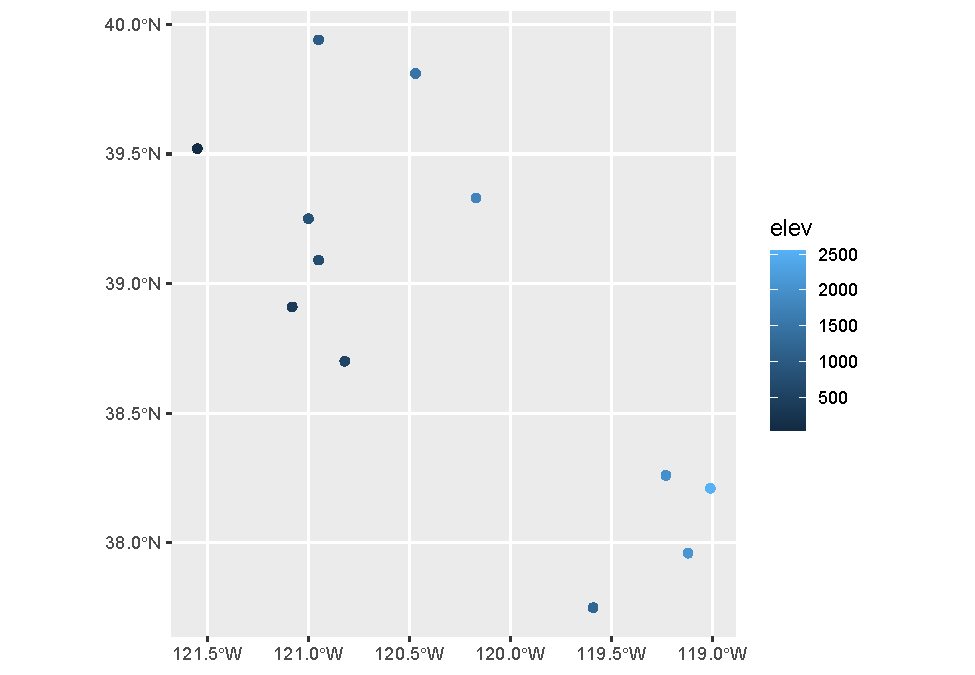
\includegraphics[width=0.75\linewidth]{EnvDataScience_files/figure-latex/mapsPtsBySF-1} 

}

\caption{Points created from a dataframe with Simple Features}\label{fig:mapsPtsBySF}
\end{figure}

\subsection{\texorpdfstring{SpatVectors in \texttt{terra}}{SpatVectors in terra}}\label{spatvectors-in-terra}

\index{SpatVectors}\index{terra}We'll briefly look at another feature-based object format, the \texttt{SpatVector} from \texttt{terra}, which uses a formal S4 object definition that provides some advantages over S3 objects such as what's in most of R, though I often prefer the simpler data frame structure of simple features in \texttt{sf}. See Hijmans (\citeproc{ref-rspatial}{n.d.}) for more about SpatVectors. We'll use terra's raster capabilities a lot more, but we'll take a brief look at building and using a \texttt{SpatVector}.

We'll start with the climate data from a selection of Sierra Nevada (and some adjacent) weather stations, created above, with variables \texttt{sta}, \texttt{lon}, \texttt{lat}, \texttt{elev}, \texttt{tC}, and \texttt{prec} entered as vectors.

Then we'll build a \texttt{SpatVector} we'll call \texttt{station\_pts} from just the longitude and latitude vectors we just created:

\begin{Shaded}
\begin{Highlighting}[]
\FunctionTok{library}\NormalTok{(terra)}
\NormalTok{lonlat }\OtherTok{\textless{}{-}} \FunctionTok{cbind}\NormalTok{(lon,lat)}
\NormalTok{station\_pts }\OtherTok{\textless{}{-}} \FunctionTok{vect}\NormalTok{(lonlat)}
\end{Highlighting}
\end{Shaded}

Unlike other data sets which use a simple object model called S3, \texttt{SpatVector} data use the more formal S4 definition. SpatVectors have a rich array of properties and associated methods, which you can see in the Environment tab of RStudio, or access with \texttt{@pnt}. This is a good thing, but the \texttt{str()} function we've been using for S3 objects presents us with arguably too much information for easy understanding. But just by entering \texttt{station\_pts} on the command line we get something similar to what \texttt{str()} does with S3 data, so this might be better for seeing a few key properties:

\begin{Shaded}
\begin{Highlighting}[]
\NormalTok{station\_pts}
\end{Highlighting}
\end{Shaded}

\begin{verbatim}
## class       : SpatVector
## geometry    : points
## dimensions  : 12, 0  (geometries, attributes)
## extent      : -121.55, -119.01, 37.75, 39.94  (xmin, xmax, ymin, ymax)
## coord. ref. :
\end{verbatim}

Note that there's nothing listed for \texttt{coord.\ ref.} meaning the \index{crs coordinate referencing system}coordinate referencing system (CRS). We'll look at this more below, but for now let's change the code a bit to add this information using the PROJ-string method:

\begin{Shaded}
\begin{Highlighting}[]
\NormalTok{station\_pts }\OtherTok{\textless{}{-}} \FunctionTok{vect}\NormalTok{(lonlat, }\AttributeTok{crs =} \StringTok{"+proj=longlat +datum=WGS84"}\NormalTok{)}
\end{Highlighting}
\end{Shaded}

Of the many methods associated with these objects, one example is getting with \index{geom()}geom():

\begin{Shaded}
\begin{Highlighting}[]
\FunctionTok{geom}\NormalTok{(station\_pts)}
\end{Highlighting}
\end{Shaded}

\begin{verbatim}
##       geom part       x     y hole
##  [1,]    1    1 -121.55 39.52    0
##  [2,]    2    1 -121.08 38.91    0
##  [3,]    3    1 -120.82 38.70    0
##  [4,]    4    1 -120.95 39.09    0
##  [5,]    5    1 -121.00 39.25    0
##  [6,]    6    1 -120.95 39.94    0
##  [7,]    7    1 -119.59 37.75    0
##  [8,]    8    1 -120.47 39.81    0
##  [9,]    9    1 -120.17 39.33    0
## [10,]   10    1 -119.23 38.26    0
## [11,]   11    1 -119.12 37.96    0
## [12,]   12    1 -119.01 38.21    0
\end{verbatim}

Let's add the attributes to the original \texttt{lonlat} matrix to build a SpatVector with attributes we can see in a basic plot (Figure \ref{fig:mapsSpatVectorPtsLabels}).

\begin{Shaded}
\begin{Highlighting}[]
\NormalTok{df }\OtherTok{\textless{}{-}} \FunctionTok{data.frame}\NormalTok{(sta,elev,tC,prec)}
\NormalTok{clim }\OtherTok{\textless{}{-}} \FunctionTok{vect}\NormalTok{(lonlat, }\AttributeTok{atts=}\NormalTok{df, }\AttributeTok{crs=}\StringTok{"+proj=longlat +datum=WGS84"}\NormalTok{)}
\NormalTok{clim}
\end{Highlighting}
\end{Shaded}

\begin{verbatim}
## class       : SpatVector
## geometry    : points
## dimensions  : 12, 4  (geometries, attributes)
## extent      : -121.55, -119.01, 37.75, 39.94  (xmin, xmax, ymin, ymax)
## coord. ref. : +proj=longlat +datum=WGS84 +no_defs
## names       :         sta  elev    tC  prec
## type        :       <chr> <num> <num> <num>
## values      :    OROVILLE    52  10.7   124
##                    AUBURN   394   9.7   160
##               PLACERVILLE   564   9.2   171
##               ...
\end{verbatim}

\begin{Shaded}
\begin{Highlighting}[]
\FunctionTok{plot}\NormalTok{(clim)}
\FunctionTok{text}\NormalTok{(clim, }\AttributeTok{labels=}\StringTok{"sta"}\NormalTok{, }\AttributeTok{pos=}\DecValTok{4}\NormalTok{)}
\end{Highlighting}
\end{Shaded}

\begin{figure}

{\centering 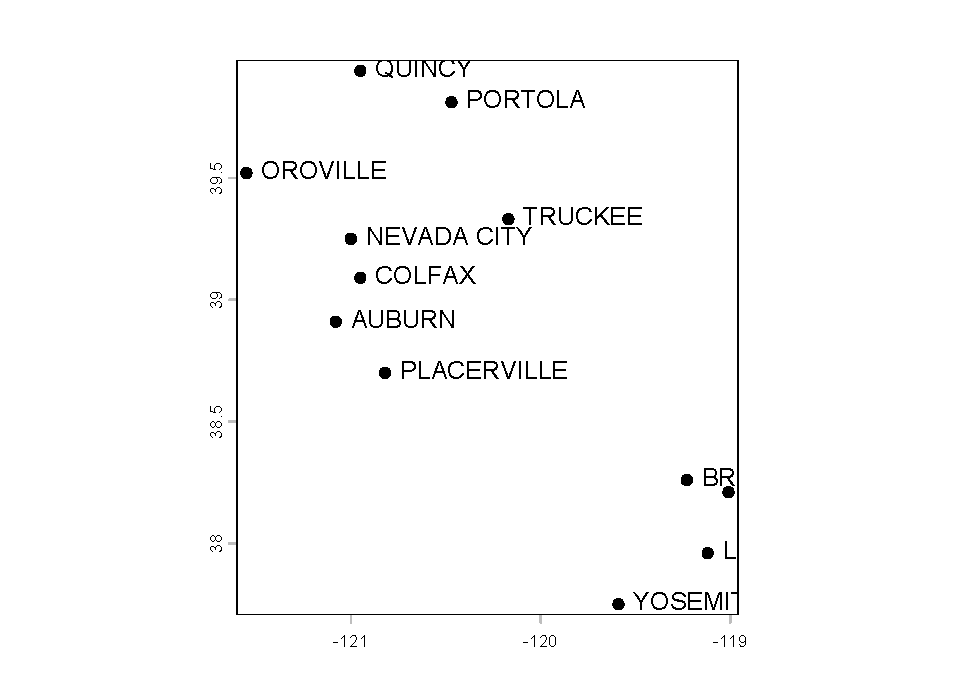
\includegraphics[width=0.75\linewidth]{EnvDataScience_files/figure-latex/mapsSpatVectorPtsLabels-1} 

}

\caption{Simple plot of SpatVector point data with labels (note that overlapping labels may result, as seen here)}\label{fig:mapsSpatVectorPtsLabels}
\end{figure}

The SpatVector format looks promising, and is increasingly supported in mapping programs like tmap, but sometimes you may want the simpler data frame + geometry structure of the \texttt{sf} model. Fortunately, you can use the \texttt{sf::sf\_as\_sf} function to convert it, just as you can create a \texttt{SpatVector} from an \texttt{sf} with the \texttt{terra::vect} function. The following code demonstrates both, with a ggplot2 map of sf data (Figure \ref{fig:mapsGG2statesStations}) and then a base R plot map with SpatVector data (Figure \ref{fig:mapsSpatVectorsPlot}).

\begin{Shaded}
\begin{Highlighting}[]
\FunctionTok{library}\NormalTok{(sf); }\FunctionTok{library}\NormalTok{(ggplot2)}
\NormalTok{climsf }\OtherTok{\textless{}{-}} \FunctionTok{st\_as\_sf}\NormalTok{(clim)}
\FunctionTok{str}\NormalTok{(climsf)}
\end{Highlighting}
\end{Shaded}

\begin{verbatim}
## Classes 'sf' and 'data.frame':   12 obs. of  5 variables:
##  $ sta     : chr  "OROVILLE" "AUBURN" "PLACERVILLE" "COLFAX" ...
##  $ elev    : num  52 394 564 725 848 ...
##  $ tC      : num  10.7 9.7 9.2 7.3 6.7 4 5 0.5 -1.1 -2.2 ...
##  $ prec    : num  124 160 171 207 268 182 169 98 126 41 ...
##  $ geometry:sfc_POINT of length 12; first list element:  'XY' num  -121.5 39.5
##  - attr(*, "sf_column")= chr "geometry"
##  - attr(*, "agr")= Factor w/ 3 levels "constant","aggregate",..: NA NA NA NA
##   ..- attr(*, "names")= chr [1:4] "sta" "elev" "tC" "prec"
\end{verbatim}

\begin{Shaded}
\begin{Highlighting}[]
\FunctionTok{ggplot}\NormalTok{() }\SpecialCharTok{+} \FunctionTok{geom\_sf}\NormalTok{(}\AttributeTok{data=}\NormalTok{twostates) }\SpecialCharTok{+} \FunctionTok{geom\_sf}\NormalTok{(}\AttributeTok{data=}\NormalTok{climsf)}
\end{Highlighting}
\end{Shaded}

\begin{figure}

{\centering 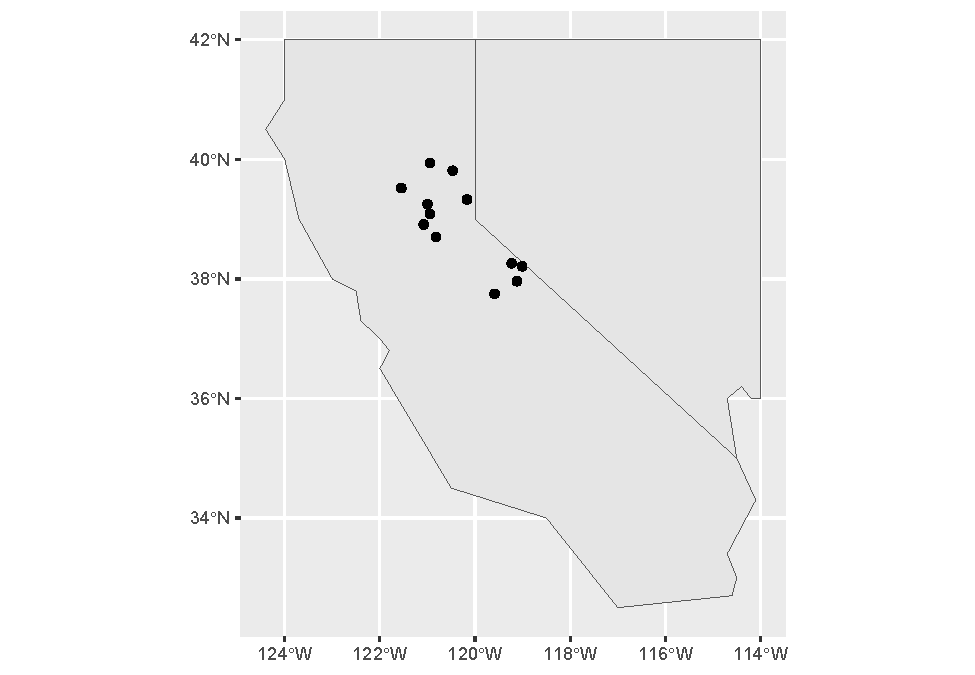
\includegraphics[width=0.75\linewidth]{EnvDataScience_files/figure-latex/mapsGG2statesStations-1} 

}

\caption{ggplot of twostates and stations}\label{fig:mapsGG2statesStations}
\end{figure}

\begin{Shaded}
\begin{Highlighting}[]
\NormalTok{twostatesV }\OtherTok{\textless{}{-}} \FunctionTok{vect}\NormalTok{(twostates)}
\FunctionTok{plot}\NormalTok{(twostatesV)}
\FunctionTok{plot}\NormalTok{(clim, }\AttributeTok{add =}\NormalTok{ T)}
\end{Highlighting}
\end{Shaded}

\begin{figure}

{\centering 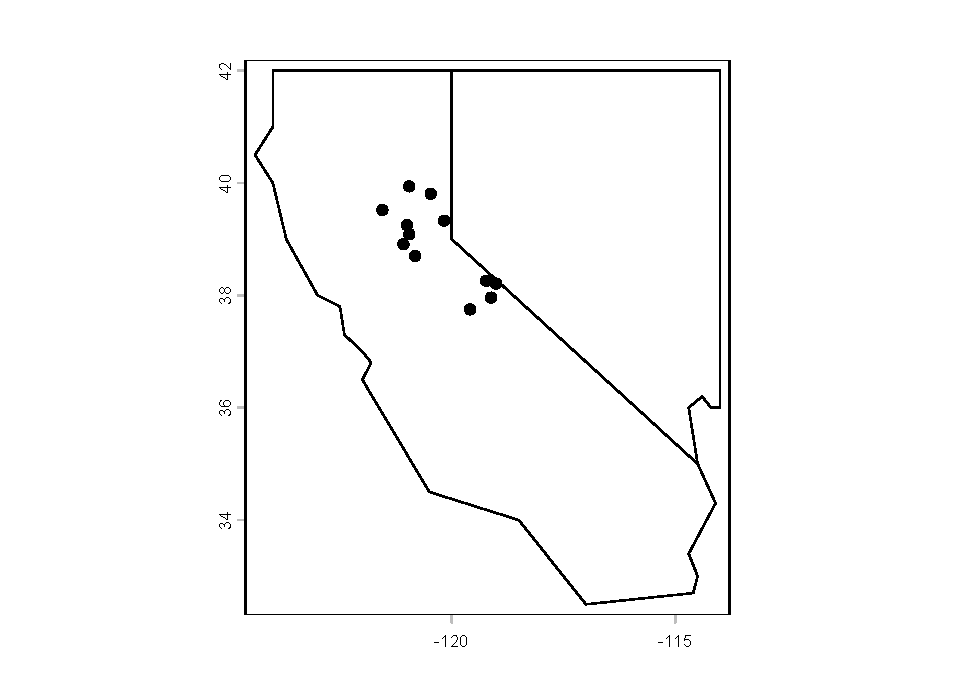
\includegraphics[width=0.75\linewidth]{EnvDataScience_files/figure-latex/mapsSpatVectorsPlot-1} 

}

\caption{Base R plot of twostates and stations SpatVectors}\label{fig:mapsSpatVectorsPlot}
\end{figure}

\begin{Shaded}
\begin{Highlighting}[]
\NormalTok{twostatesV}
\end{Highlighting}
\end{Shaded}

\begin{verbatim}
## class       : SpatVector
## geometry    : polygons
## dimensions  : 2, 3  (geometries, attributes)
## extent      : -124.4, -114, 32.5, 42  (xmin, xmax, ymin, ymax)
## coord. ref. : lon/lat WGS 84 (EPSG:4326)
## names       :   abb   area       pop
## type        : <chr>  <num>     <num>
## values      :    CA 423970 3.956e+07
##                  NV 286382  3.03e+06
\end{verbatim}

\subsection{Creating features from shapefiles}\label{creating-features-from-shapefiles}

Both sf's \index{st\_read}\texttt{st\_read} and terra's \index{vect}\texttt{vect} read the open-GIS \index{shapefile}\emph{shapefile} format developed by Esri for points, polylines, and polygons. You would normally have shapefiles (and all the files that go with them -- .shx, etc.) stored on your computer, but we'll access one from the \texttt{igisci} external data folder, and use that \texttt{ex()} function we used earlier with CSVs. \emph{Remember that we could just include that and the library calls just once at the top of our code like this\ldots{}}

\begin{Shaded}
\begin{Highlighting}[]
\FunctionTok{library}\NormalTok{(igisci)}
\FunctionTok{library}\NormalTok{(sf)}
\end{Highlighting}
\end{Shaded}

If we just send a spatial dataset like an \texttt{sf} spatial data frame to the plot system, it will plot all of the variables by default (Figure \ref{fig:mapsPlotBayAreaCo}).

\begin{Shaded}
\begin{Highlighting}[]
\NormalTok{BayAreaCounties }\OtherTok{\textless{}{-}} \FunctionTok{st\_read}\NormalTok{(}\FunctionTok{ex}\NormalTok{(}\StringTok{"BayArea/BayAreaCounties.shp"}\NormalTok{))}
\end{Highlighting}
\end{Shaded}

\begin{Shaded}
\begin{Highlighting}[]
\FunctionTok{plot}\NormalTok{(BayAreaCounties)}
\end{Highlighting}
\end{Shaded}

\begin{figure}

{\centering 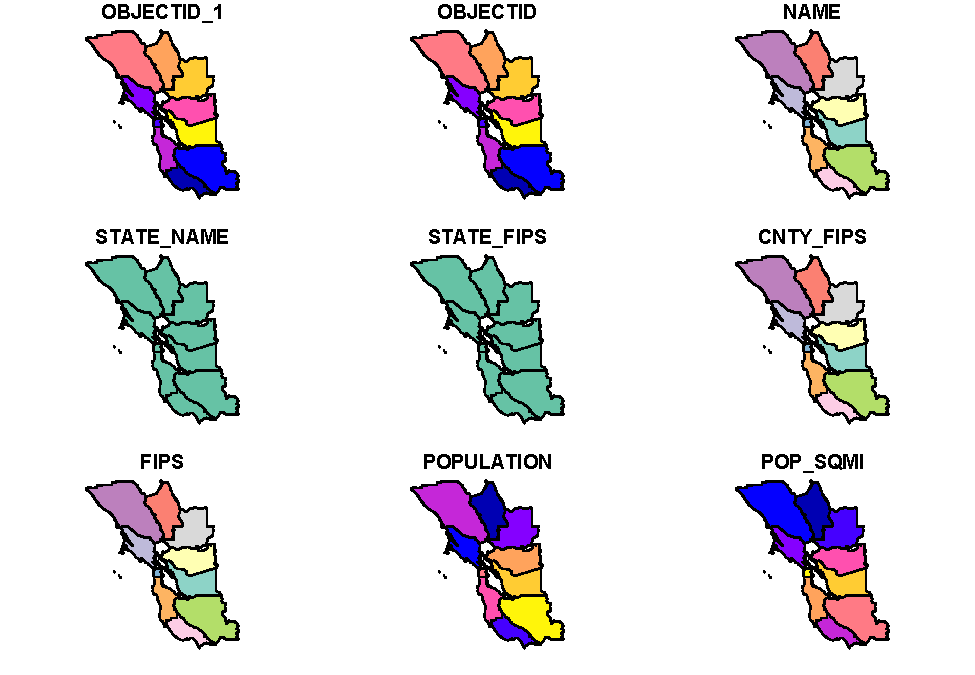
\includegraphics[width=0.75\linewidth]{EnvDataScience_files/figure-latex/mapsPlotBayAreaCo-1} 

}

\caption{A simple plot of polygon data by default shows all variables}\label{fig:mapsPlotBayAreaCo}
\end{figure}

But with just one variable, of course, it just produces a single map (Figure \ref{fig:mapsBayAreaCo1var}).

\begin{Shaded}
\begin{Highlighting}[]
\FunctionTok{plot}\NormalTok{(BayAreaCounties[}\StringTok{"POPULATION"}\NormalTok{])}
\end{Highlighting}
\end{Shaded}

\begin{figure}

{\centering 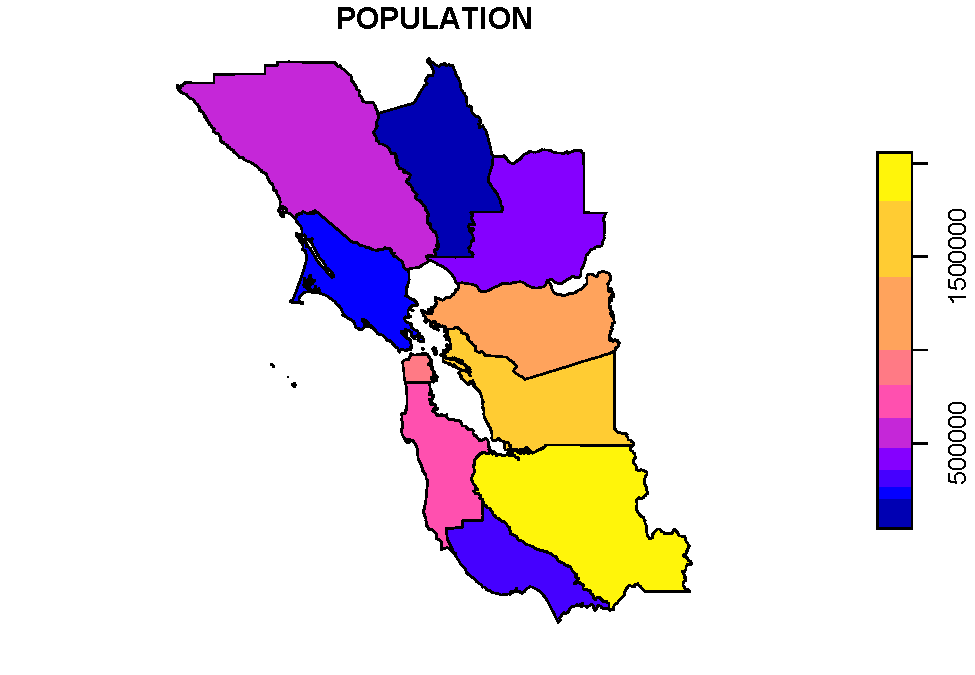
\includegraphics[width=0.75\linewidth]{EnvDataScience_files/figure-latex/mapsBayAreaCo1var-1} 

}

\caption{A single map with a legend is produced when a variable is specified}\label{fig:mapsBayAreaCo1var}
\end{figure}

Notice that in the above map, we used the \texttt{{[}{]}} accessor. Why didn't we use the simple \texttt{\$} accessor? Remember that plot() figures out what to do based on what you provide it. And there's an important difference in what you get with the two accessors, which we can check with class():

\begin{Shaded}
\begin{Highlighting}[]
\FunctionTok{class}\NormalTok{(BayAreaCounties[}\StringTok{"POPULATION"}\NormalTok{])}
\end{Highlighting}
\end{Shaded}

\begin{verbatim}
## [1] "sf"         "data.frame"
\end{verbatim}

\begin{Shaded}
\begin{Highlighting}[]
\FunctionTok{class}\NormalTok{(BayAreaCounties}\SpecialCharTok{$}\NormalTok{POPULATION)}
\end{Highlighting}
\end{Shaded}

\begin{verbatim}
## [1] "numeric"
\end{verbatim}

You might see that what you get with \texttt{plot(BayAreaCounties\$POPULATION)} is not very informative, since the object is just a numeric vector, while using \texttt{{[}{]}} accessor returns a spatial dataframe.

There's a lot more we could do with the base R plot system, so we'll learn some of these before exploring what we can do with \texttt{ggplot2}, \texttt{tmap}, and \texttt{leaflet}. But first we need to learn more about building geospatial data.

We'll use \texttt{st\_as\_sf()} for that, but we'll need to specify the coordinate referencing system (CRS), in this case GCS. We'll only briefly explore how to specify the CRS here. For a thorough coverage, please see Lovelace et al. (\citeproc{ref-Geocomputation}{2019}).

\section{Coordinate Referencing Systems}\label{coordinate-referencing-systems}

\index{coordinate referencing systems crs}Before we try the next method for bringing in spatial data -- converting data frames -- we need to look at coordinate referencing systems (CRS). First, there are quite a few, with some spherical like the geographic coordinate system (GCS) of longitude and latitude, and others planar projections of GCS using mathematically defined projections such as Mercator, Albers Conformal Conic, Azimuthal, etc., and including widely used government-developed systems such as UTM (universal transverse mercator) or state plane. Even for GCS, there are many varieties since geodetic datums can be chosen, and for very fine resolution work where centimetres or even millimetres matter, this decision can be important (and tectonic plate movement can play havoc with tying it down.)

There are also multiple ways of expressing the CRS, either to read it or to set it. The full specification of a CRS can be displayed for data already in a CRS, with either \index{st\_crs}\texttt{sf::st\_crs} or \index{crs, terra}\texttt{terra::crs}.

\begin{Shaded}
\begin{Highlighting}[]
\FunctionTok{st\_crs}\NormalTok{(CA\_counties)}
\end{Highlighting}
\end{Shaded}

\begin{verbatim}
## Coordinate Reference System:
##   User input: WGS 84 
##   wkt:
## GEOGCRS["WGS 84",
##     DATUM["World Geodetic System 1984",
##         ELLIPSOID["WGS 84",6378137,298.257223563,
##             LENGTHUNIT["metre",1]]],
##     PRIMEM["Greenwich",0,
##         ANGLEUNIT["degree",0.0174532925199433]],
##     CS[ellipsoidal,2],
##         AXIS["latitude",north,
##             ORDER[1],
##             ANGLEUNIT["degree",0.0174532925199433]],
##         AXIS["longitude",east,
##             ORDER[2],
##             ANGLEUNIT["degree",0.0174532925199433]],
##     ID["EPSG",4326]]
\end{verbatim}

\ldots{} though there are other ways to see the crs in shorter forms, or its individual properties :

\begin{Shaded}
\begin{Highlighting}[]
\FunctionTok{st\_crs}\NormalTok{(CA\_counties)}\SpecialCharTok{$}\NormalTok{proj4string}
\end{Highlighting}
\end{Shaded}

\begin{verbatim}
## [1] "+proj=longlat +datum=WGS84 +no_defs"
\end{verbatim}

\begin{Shaded}
\begin{Highlighting}[]
\FunctionTok{st\_crs}\NormalTok{(CA\_counties)}\SpecialCharTok{$}\NormalTok{units\_gdal}
\end{Highlighting}
\end{Shaded}

\begin{verbatim}
## [1] "degree"
\end{verbatim}

\begin{Shaded}
\begin{Highlighting}[]
\FunctionTok{st\_crs}\NormalTok{(CA\_counties)}\SpecialCharTok{$}\NormalTok{epsg}
\end{Highlighting}
\end{Shaded}

\begin{verbatim}
## [1] 4326
\end{verbatim}

\begin{quote}
There's also \texttt{st\_crs()\$Wkt}, which you should try, but it creates a long, continuous string that goes off the page, so doesn't work for the book formatting.
\end{quote}

\begin{Shaded}
\begin{Highlighting}[]
\FunctionTok{st\_crs}\NormalTok{(CA\_counties)}\SpecialCharTok{$}\NormalTok{Wkt }\CommentTok{\# [Creates too long of a string for this book]}
\end{Highlighting}
\end{Shaded}

So, to convert the sierra data into \index{st\_as\_sf}geospatial data with \texttt{st\_as\_sf}, we might either do it with the reasonably short PROJ format \ldots{}

\begin{verbatim}
GCS <- "+proj=longlat +datum=WGS84 +no_defs +ellps=WGS84 +towgs84=0,0,0"
wsta = st_as_sf(sierraFeb, coords = c("LONGITUDE","LATITUDE"), crs=GCS)
\end{verbatim}

\ldots{} or with the even shorter EPSG code (which we can find by Googling), which can either be provided as text \texttt{"epsg:4326"} or often just the number, which we'll use next.

\section{Creating sf Data from Data Frames}\label{creating-sf-data-from-data-frames}

\index{sf data from data frames}As we saw earlier, if your data frame has geospatial coordinates like \texttt{LONGITUDE} and \texttt{LATITUDE} \ldots{}

\begin{Shaded}
\begin{Highlighting}[]
\FunctionTok{names}\NormalTok{(sierraFeb)}
\end{Highlighting}
\end{Shaded}

\begin{verbatim}
## [1] "STATION_NAME"  "COUNTY"        "ELEVATION"     "LATITUDE"     
## [5] "LONGITUDE"     "PRECIPITATION" "TEMPERATURE"
\end{verbatim}

\ldots{} we have what we need to create geospatial data from it. Earlier we read in a series of vectors built in code with \texttt{c()} functions from 12 selected weather stations; this time we'll use a data frame that has all of the Sierra Nevada weather stations (Figure \ref{fig:mapsPtsCreatedFromDF}).

\begin{Shaded}
\begin{Highlighting}[]
\NormalTok{wsta }\OtherTok{\textless{}{-}} \FunctionTok{st\_as\_sf}\NormalTok{(sierraFeb, }\AttributeTok{coords =} \FunctionTok{c}\NormalTok{(}\StringTok{"LONGITUDE"}\NormalTok{,}\StringTok{"LATITUDE"}\NormalTok{), }\AttributeTok{crs=}\DecValTok{4326}\NormalTok{)}
\FunctionTok{ggplot}\NormalTok{(}\AttributeTok{data=}\NormalTok{wsta) }\SpecialCharTok{+} \FunctionTok{geom\_sf}\NormalTok{(}\FunctionTok{aes}\NormalTok{(}\AttributeTok{col=}\NormalTok{ELEVATION))}
\end{Highlighting}
\end{Shaded}

\begin{figure}

{\centering 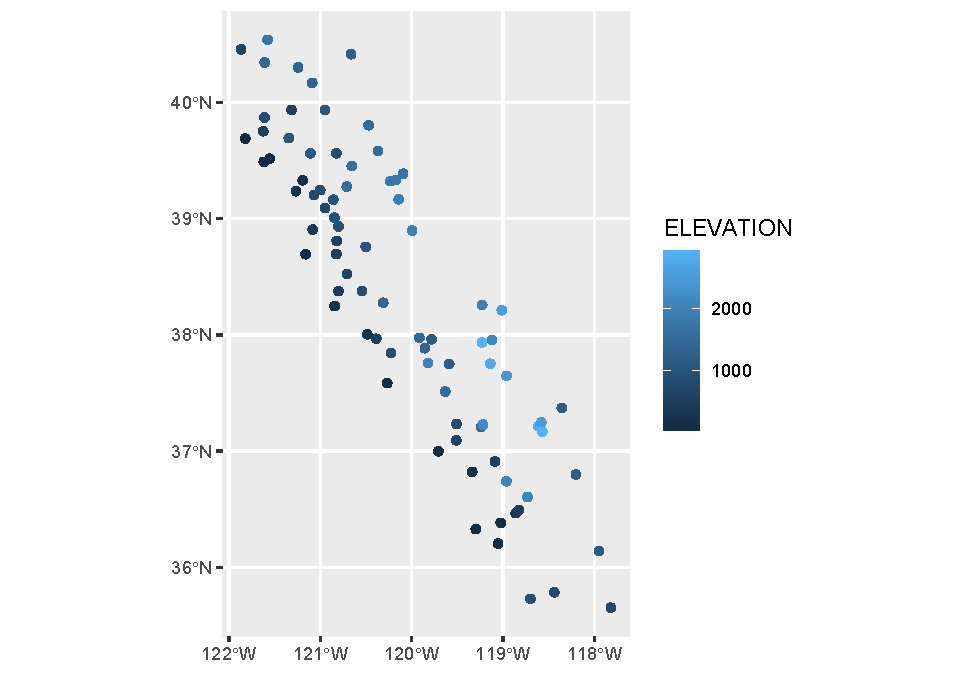
\includegraphics[width=0.75\linewidth]{EnvDataScience_files/figure-latex/mapsPtsCreatedFromDF-1} 

}

\caption{Points created from data frame with coordinate variables}\label{fig:mapsPtsCreatedFromDF}
\end{figure}

\subsection{\texorpdfstring{\emph{Removing} geometry}{Removing geometry}}\label{removing-geometry}

\index{geometry, removing}There are many instances where you want to remove geometry from a sf data frame.

\begin{itemize}
\item
  Some R functions run into problems with geometry and produce confusing error messages, like ``non-numeric argument''
\item
  To work with an sf data frame in a non-spatial way
\end{itemize}

One way to remove geometry \index{st\_set\_geometry}:

\texttt{myNonSFdf\ \textless{}-\ mySFdf\ \%\textgreater{}\%\ st\_set\_geometry(NULL)}

\section{\texorpdfstring{Base R's \texttt{plot()} with \texttt{terra}}{Base R's plot() with terra}}\label{base-rs-plot-with-terra}

\index{plot with terra}As we've seen in the examples above, the venerable plot system in base R can often do a reasonable job of displaying a map. The terra package extends this a bit by providing tools for overlaying features on other features (or rasters using plotRGB), so it's often easy to use (Figure \ref{fig:mapsSpatVectorData}).

\begin{Shaded}
\begin{Highlighting}[]
\FunctionTok{library}\NormalTok{(terra)}
\FunctionTok{plot}\NormalTok{(}\FunctionTok{vect}\NormalTok{(wsta))}
\FunctionTok{lines}\NormalTok{(}\FunctionTok{vect}\NormalTok{(CA\_counties), }\AttributeTok{col=}\StringTok{"gray"}\NormalTok{)}
\end{Highlighting}
\end{Shaded}

\begin{figure}

{\centering 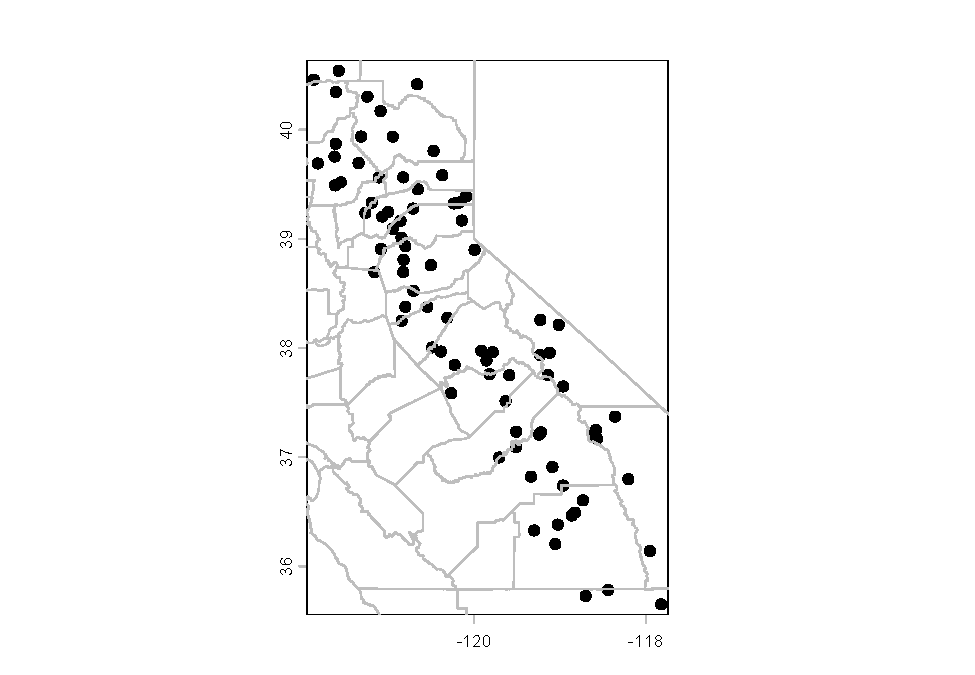
\includegraphics[width=0.75\linewidth]{EnvDataScience_files/figure-latex/mapsSpatVectorData-1} 

}

\caption{Plotting SpatVector data with base R plot system}\label{fig:mapsSpatVectorData}
\end{figure}

Note that we converted the sf data to \texttt{terra} \texttt{SpatVector} data with \texttt{vect()}, but the base R plot system can work with either \texttt{sf} data or \texttt{SpatVector} data from \texttt{terra}.

The \texttt{lines}, \texttt{points}, and \texttt{polys} functions (to name a few -- see \texttt{?terra} and look at the Plotting section) will add to an existing plot. Alternatively, we could use plot's \texttt{add=TRUE} parameter to add onto a plot that we've previously scaled with a plot. In this case, we'll cheat and just use the first plot to set the scaling but then cover over that plot with other plots (Figure \ref{fig:mapsBaseRaddTRUE}).

\begin{Shaded}
\begin{Highlighting}[]
\FunctionTok{library}\NormalTok{(terra)}
\FunctionTok{plot}\NormalTok{(}\FunctionTok{vect}\NormalTok{(wsta[}\DecValTok{1}\NormalTok{])) }\CommentTok{\# simple way of establishing the coordinates}
\CommentTok{\# Then will be covered by the following:}
\FunctionTok{plot}\NormalTok{(}\FunctionTok{vect}\NormalTok{(CA\_counties), }\AttributeTok{col=}\StringTok{"lightgray"}\NormalTok{, }\AttributeTok{add=}\ConstantTok{TRUE}\NormalTok{)}
\FunctionTok{plot}\NormalTok{(}\FunctionTok{vect}\NormalTok{(wsta), }\AttributeTok{col=}\StringTok{"red"}\NormalTok{, }\AttributeTok{add=}\ConstantTok{TRUE}\NormalTok{)}
\end{Highlighting}
\end{Shaded}

\begin{figure}

{\centering 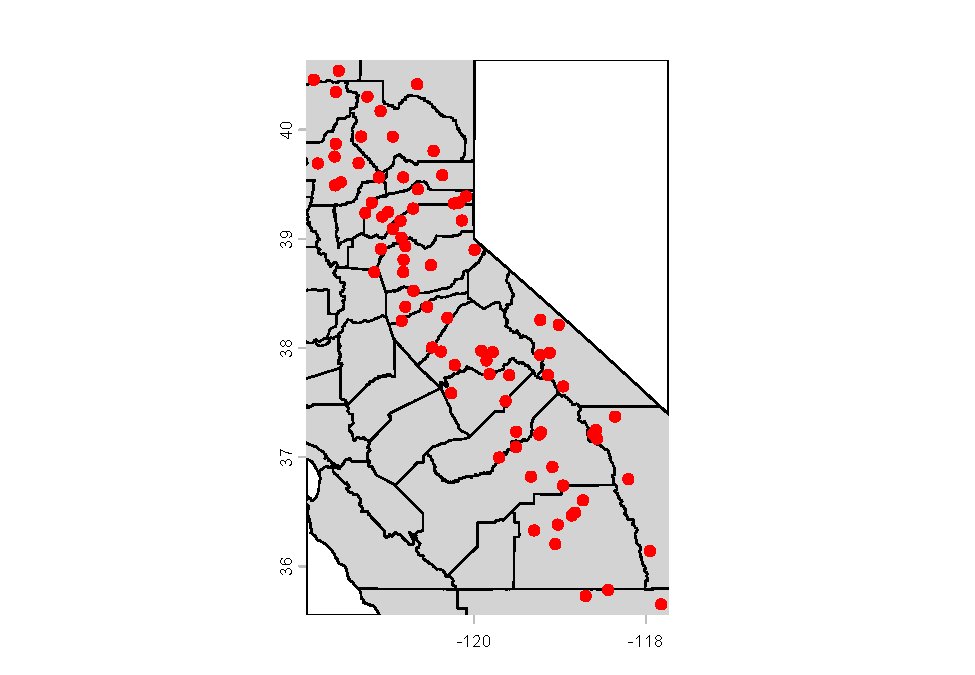
\includegraphics[width=0.75\linewidth]{EnvDataScience_files/figure-latex/mapsBaseRaddTRUE-1} 

}

\caption{Features added to the map using the base R plot system}\label{fig:mapsBaseRaddTRUE}
\end{figure}

\subsection{Using maptiles to create a basemap}\label{using-maptiles-to-create-a-basemap}

\index{maptiles}For vector data, it's often nice to display over a \index{basemap}basemap by accessing raster tiles that are served on the internet by various providers. We'll use the \texttt{maptiles} package to try displaying the \texttt{CA} and \texttt{NV} boundaries we created earlier. The \texttt{maptiles} package supports a variety of basemap providers, and I've gotten the following to work: \texttt{"OpenStreetMap"}, \texttt{"Stamen.Terrain"}, \texttt{"Stamen.TerrainBackground"}, \texttt{"Esri.WorldShadedRelief"}, \texttt{"Esri.NatGeoWorldMap"}, \texttt{"Esri.WorldGrayCanvas"}, \texttt{"CartoDB.Positron"}, \texttt{"CartoDB.Voyager"}, \texttt{"CartoDB.DarkMatter"}, \texttt{"OpenTopoMap"}, \texttt{"Wikimedia"}, \emph{however, they don't work at all scales and locations -- you'll often see an Error in grDevices, if so then try another provider -- the default \texttt{"OpenStreetMap"} seems to work the most reliably} (Figure \ref{fig:mapsMaptiles}).

\begin{Shaded}
\begin{Highlighting}[]
\FunctionTok{library}\NormalTok{(terra); }\FunctionTok{library}\NormalTok{(maptiles)}
\CommentTok{\# Get the raster that covers the extent of CANV:}
\NormalTok{calnevaBase }\OtherTok{\textless{}{-}} \FunctionTok{get\_tiles}\NormalTok{(twostates, }\AttributeTok{provider=}\StringTok{"Esri.NatGeoWorldMap"}\NormalTok{) }\CommentTok{\#OpenTopoMap")}
\FunctionTok{st\_crs}\NormalTok{(twostates)}\SpecialCharTok{$}\NormalTok{epsg}
\end{Highlighting}
\end{Shaded}

\begin{verbatim}
## [1] 4326
\end{verbatim}

\begin{Shaded}
\begin{Highlighting}[]
\FunctionTok{plotRGB}\NormalTok{(calnevaBase)  }\CommentTok{\# starts plot with a raster basemap}
\FunctionTok{lines}\NormalTok{(}\FunctionTok{vect}\NormalTok{(twostates), }\AttributeTok{col=}\StringTok{"black"}\NormalTok{, }\AttributeTok{lwd=}\DecValTok{2}\NormalTok{)}
\end{Highlighting}
\end{Shaded}

\begin{figure}

{\centering 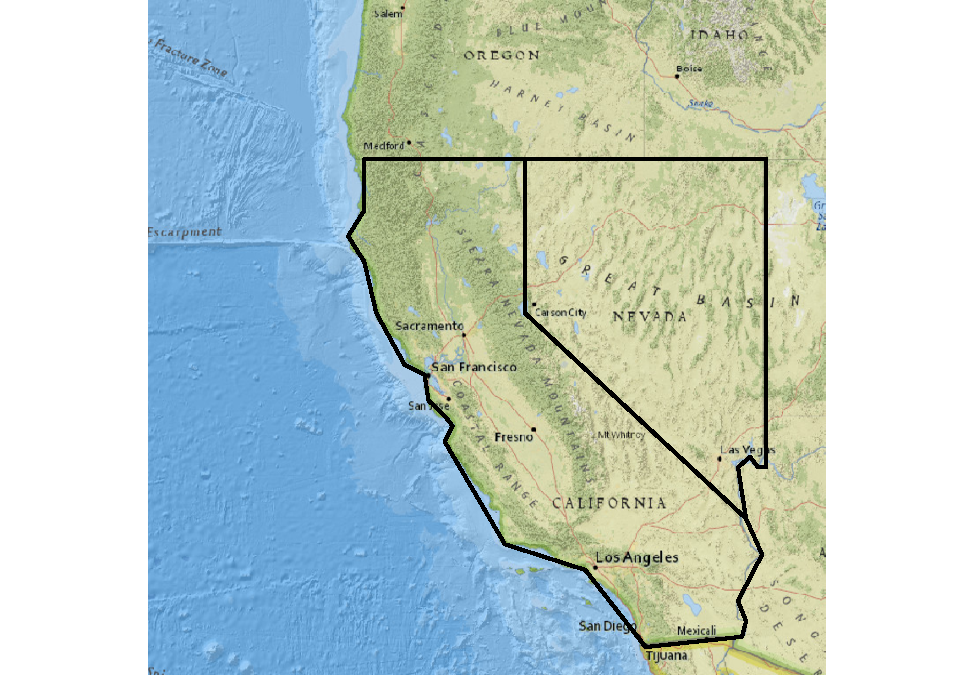
\includegraphics[width=0.75\linewidth]{EnvDataScience_files/figure-latex/mapsMaptiles-1} 

}

\caption{Using maptiles for a base map}\label{fig:mapsMaptiles}
\end{figure}

In the code above, we can also see the use of \texttt{terra} functions and parameters. Learn more about these by reviewing the code and considering:

\textbf{terra functions}: The \texttt{terra::vect()} function creates a \texttt{SpatVector} that works with \texttt{terra::lines} to display the boundary lines in \texttt{plot()}. (More on \texttt{terra} later, in the Raster section.)

\textbf{parameters}: Note the use of the parameter \texttt{lwd} (line width) from the plot system. This is one of \emph{many} parameter settings described in \textbf{\texttt{?par}}. It defaults to 1, so 2 makes it twice as thick. You could also use lty (line type) to change it to a dashed line with \texttt{lty="dashed"} or \texttt{lty=2}.

And for the \texttt{sierraFeb} data, we'll start with \texttt{st\_as\_sf} and the coordinate system (4326 for GCS), then use a \texttt{maptiles} basemap again, and the \texttt{terra::points} method to add the points (Figure \ref{fig:mapsConvertedSF4tiles}).

\begin{Shaded}
\begin{Highlighting}[]
\FunctionTok{library}\NormalTok{(terra); }\FunctionTok{library}\NormalTok{(maptiles)}
\NormalTok{sierraFebpts }\OtherTok{\textless{}{-}} \FunctionTok{st\_as\_sf}\NormalTok{(sierraFeb, }\AttributeTok{coords =} \FunctionTok{c}\NormalTok{(}\StringTok{"LONGITUDE"}\NormalTok{, }\StringTok{"LATITUDE"}\NormalTok{), }\AttributeTok{crs=}\DecValTok{4326}\NormalTok{)}
\NormalTok{sierraBase }\OtherTok{\textless{}{-}} \FunctionTok{get\_tiles}\NormalTok{(sierraFebpts)}
\FunctionTok{st\_crs}\NormalTok{(sierraFebpts)}\SpecialCharTok{$}\NormalTok{epsg}
\end{Highlighting}
\end{Shaded}

\begin{verbatim}
## [1] 4326
\end{verbatim}

\begin{Shaded}
\begin{Highlighting}[]
\FunctionTok{plotRGB}\NormalTok{(sierraBase)}
\FunctionTok{points}\NormalTok{(}\FunctionTok{vect}\NormalTok{(sierraFebpts))}
\end{Highlighting}
\end{Shaded}

\begin{figure}

{\centering 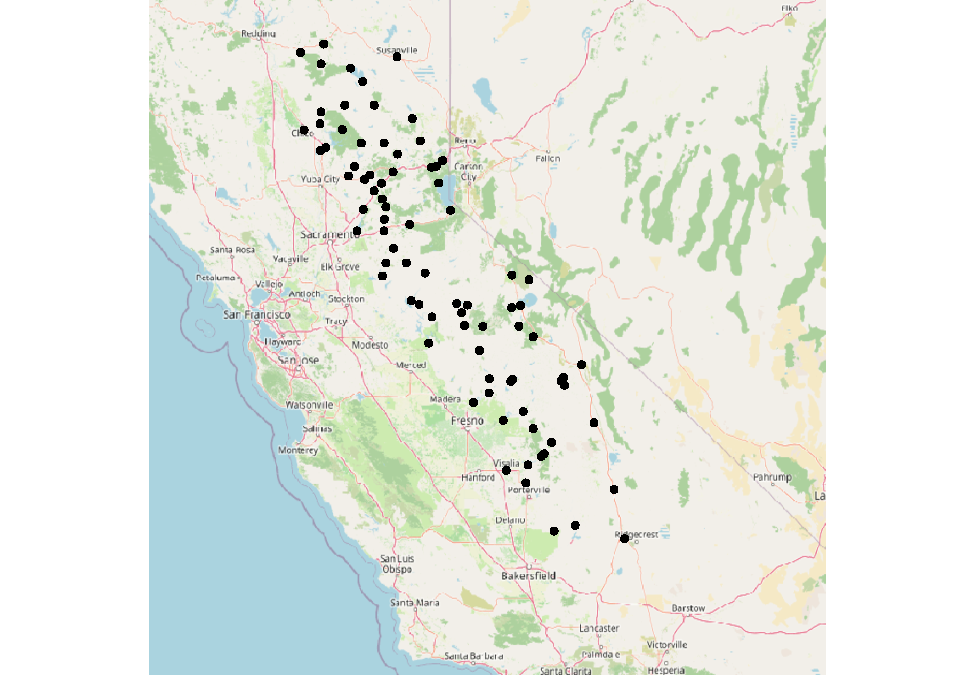
\includegraphics[width=0.75\linewidth]{EnvDataScience_files/figure-latex/mapsConvertedSF4tiles-1} 

}

\caption{Converted sf data for map with tiles}\label{fig:mapsConvertedSF4tiles}
\end{figure}

\begin{quote}
We'll learn another way to use basemaps in tmap, later in the chapter, but it uses the same source of basemaps.
\end{quote}

\section{Raster data}\label{raster-data}

\index{raster data}Simple \emph{Features} are feature-based, of course, so it's not surprising that \texttt{sf} doesn't have support for rasters. So we'll want to either use the \texttt{raster} package or its imminent replacement, \texttt{terra} (which also has vector methods -- see Hijmans (\citeproc{ref-rspatial}{n.d.}) and Lovelace et al. (\citeproc{ref-Geocomputation}{2019}))\index{terra}, and I'm increasingly using \texttt{terra} since it has some improvements that I find useful.

\subsection{Building rasters}\label{building-rasters}

We can start by building one from scratch. The \texttt{terra} package has a \texttt{rast()} function \index{rast}for this, and creates an S4 (as opposed to the simpler S3) object type called a \texttt{SpatRaster}.

\begin{Shaded}
\begin{Highlighting}[]
\FunctionTok{library}\NormalTok{(terra)}
\NormalTok{new\_ras }\OtherTok{\textless{}{-}} \FunctionTok{rast}\NormalTok{(}\AttributeTok{ncol =} \DecValTok{12}\NormalTok{, }\AttributeTok{nrow =} \DecValTok{6}\NormalTok{,}
                \AttributeTok{xmin =} \SpecialCharTok{{-}}\DecValTok{180}\NormalTok{, }\AttributeTok{xmax =} \DecValTok{180}\NormalTok{, }\AttributeTok{ymin =} \SpecialCharTok{{-}}\DecValTok{90}\NormalTok{, }\AttributeTok{ymax =} \DecValTok{90}\NormalTok{,}
                \AttributeTok{vals =} \DecValTok{1}\SpecialCharTok{:}\DecValTok{72}\NormalTok{)}
\end{Highlighting}
\end{Shaded}

Formal S4 objects like \texttt{SpatRasters} have many associated properties and methods. To get a sense, type into the console \texttt{new\_ras@pnt\$} and see what suggestions you get from the autocomplete system. To learn more about them, see Hijmans (\citeproc{ref-rspatial}{n.d.}), but we'll look at a few of the key properties by simply entering the \texttt{SpatRaster} name in the console.

\begin{Shaded}
\begin{Highlighting}[]
\NormalTok{new\_ras}
\end{Highlighting}
\end{Shaded}

\begin{verbatim}
## class       : SpatRaster
## size        : 6, 12, 1  (nrow, ncol, nlyr)
## resolution  : 30, 30  (x, y)
## extent      : -180, 180, -90, 90  (xmin, xmax, ymin, ymax)
## coord. ref. : lon/lat WGS 84 (CRS84) (OGC:CRS84)
## source(s)   : memory
## name        : lyr.1
## min value   :     1
## max value   :    72
\end{verbatim}

\begin{itemize}
\tightlist
\item
  The \texttt{nrow} and \texttt{ncol} dimensions should be familiar, and the \texttt{nlyr} tells us that this raster has a single layer (or band as they're referred to with imagery), and it gives it the name \texttt{lyr.1}.
\item
  The resolution is what you get when you divide 360 (degrees of longitude) by 12 and 180 (degrees of latitude) by 6, and the extent is what we entered to create it.
\item
  But how does it know that these are degrees of longitude and latitude, as it appears to from the \texttt{coord.\ ref.} property? The author of this tool seems to let it assume GCS if it doesn't exceed the limits of the planet: -180 to +180 longitude and -90 to +90 latitude.
\item
  The source is in memory, since we didn't read it from a file, but entered it directly. New rasters we might create from raster operations will also be in memory.
\item
  The minimum and maximum values are what we used to create it.
\end{itemize}

The name \texttt{lyr.1} isn't very useful, so let's change the name with the \texttt{names} function, and then access the name with a \texttt{@pnt} property (you could also use \texttt{names(new\_ras)} to access it, but I thought it might be useful to see the \texttt{@pnt} in action.)

\begin{Shaded}
\begin{Highlighting}[]
\FunctionTok{names}\NormalTok{(new\_ras) }\OtherTok{\textless{}{-}} \StringTok{"world30deg"}
\NormalTok{new\_ras}
\end{Highlighting}
\end{Shaded}

\begin{verbatim}
## class       : SpatRaster
## size        : 6, 12, 1  (nrow, ncol, nlyr)
## resolution  : 30, 30  (x, y)
## extent      : -180, 180, -90, 90  (xmin, xmax, ymin, ymax)
## coord. ref. : lon/lat WGS 84 (CRS84) (OGC:CRS84)
## source(s)   : memory
## name        : world30deg
## min value   :          1
## max value   :         72
\end{verbatim}

Simple feature data or \texttt{SpatVectors} can be plotted along with rasters using terra's lines, polys, or points functions. Here we'll use the \texttt{twostates} \texttt{sf} we created earlier (make sure to run that code again if you need it). Look closely at the map for our two states (Figure \ref{fig:mapsSpatRasterSpatVector}).

\begin{Shaded}
\begin{Highlighting}[]
\FunctionTok{plot}\NormalTok{(new\_ras, }\AttributeTok{main=}\FunctionTok{paste}\NormalTok{(}\StringTok{"CANV on"}\NormalTok{,new\_ras}\SpecialCharTok{@}\NormalTok{pntr}\SpecialCharTok{$}\NormalTok{names))}
\NormalTok{CANV }\OtherTok{\textless{}{-}} \FunctionTok{vect}\NormalTok{(twostates)}
\FunctionTok{lines}\NormalTok{(CANV)}
\end{Highlighting}
\end{Shaded}

\begin{figure}

{\centering 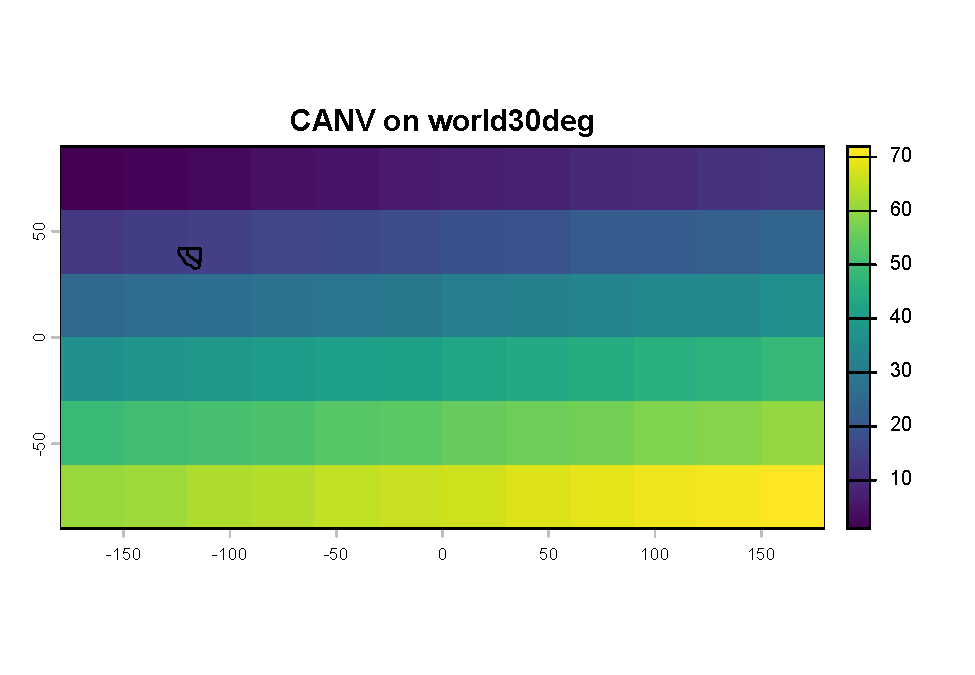
\includegraphics[width=0.75\linewidth]{EnvDataScience_files/figure-latex/mapsSpatRasterSpatVector-1} 

}

\caption{Simple plot of a worldwide SpatRaster of 30-degree cells, with SpatVector of CA and NV added}\label{fig:mapsSpatRasterSpatVector}
\end{figure}

\subsection{Vector to raster conversion}\label{vector-to-raster-conversion}

\index{vector to raster conversion} To convert rasters to vectors requires having a template raster with the desired cell size and extent, or an existing raster we can use as a template -- we ignore what the values are -- such as \texttt{elev.tif} in the following example (Figure \ref{fig:mapsStrRas}):

\begin{Shaded}
\begin{Highlighting}[]
\NormalTok{streams }\OtherTok{\textless{}{-}} \FunctionTok{vect}\NormalTok{(}\FunctionTok{ex}\NormalTok{(}\StringTok{"marbles/streams.shp"}\NormalTok{))}
\NormalTok{elev }\OtherTok{\textless{}{-}} \FunctionTok{rast}\NormalTok{(}\FunctionTok{ex}\NormalTok{(}\StringTok{"marbles/elev.tif"}\NormalTok{))}
\NormalTok{streamras }\OtherTok{\textless{}{-}} \FunctionTok{rasterize}\NormalTok{(streams,elev)}
\FunctionTok{plot}\NormalTok{(streamras, }\AttributeTok{col=}\StringTok{"blue"}\NormalTok{)}
\end{Highlighting}
\end{Shaded}

\begin{figure}

{\centering 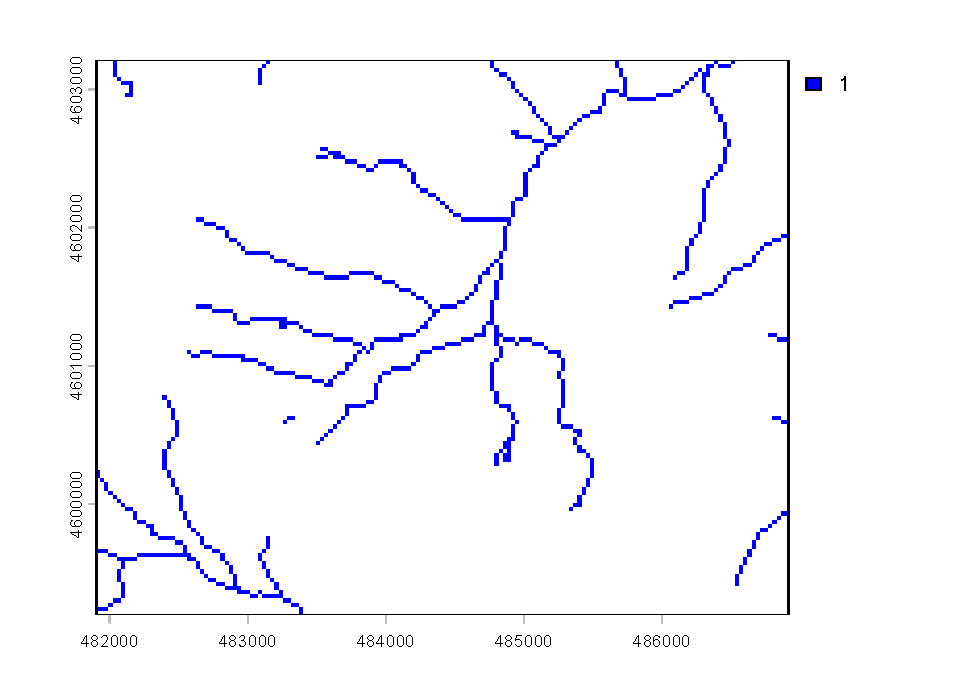
\includegraphics[width=0.75\linewidth]{EnvDataScience_files/figure-latex/mapsStrRas-1} 

}

\caption{Stream raster converted from stream features, with 30 m cells from an elevation raster template}\label{fig:mapsStrRas}
\end{figure}

\subsubsection{What if we have no raster to use as a template?}\label{what-if-we-have-no-raster-to-use-as-a-template}

\index{new raster from scratch}In the above process, we referenced \texttt{elev} essentially as a template to get a raster structure and crs to use. But what if we wanted to do the conversion and we didn't have a raster to use as a template? We'd need to create a raster, specifying the cell size and the extent (\texttt{xmin}, \texttt{xmax}, \texttt{ymin}, \texttt{ymax}).

If you know those extent values, you could start from scratch. But we'll look at a common situation where we have existing features, from the \texttt{streams.shp} we are wishing to rasterize\ldots{}

\begin{Shaded}
\begin{Highlighting}[]
\NormalTok{streams }\OtherTok{\textless{}{-}} \FunctionTok{vect}\NormalTok{(}\FunctionTok{ex}\NormalTok{(}\StringTok{"marbles/streams.shp"}\NormalTok{))}
\NormalTok{streams}
\end{Highlighting}
\end{Shaded}

\begin{verbatim}
## class       : SpatVector
## geometry    : lines
## dimensions  : 48, 8  (geometries, attributes)
## extent      : 481903.6, 486901.9, 4599199, 4603200  (xmin, xmax, ymin, ymax)
## source      : streams.shp
## coord. ref. : NAD83 / UTM zone 10N (EPSG:26910)
## names       : FNODE_ TNODE_ LPOLY_ RPOLY_  LENGTH STREAMS_ STREAMS_ID Shape_Leng
## type        :  <num>  <num>  <num>  <num>   <num>    <num>      <num>      <num>
## values      :      5      6      4      4 269.284        1          1    269.284
##                    2      7      2      2 153.684        2          5    153.684
##                    8      1      2      2 337.887        3         36    337.887
##               ...
\end{verbatim}

\ldots{} and in code we could pull out the four extent properties with the \index{ext}\texttt{ext()} function, and use that also to work out the aspect ratio and (assuming that we know we want a raster cell size of 30 m based on the crs being in UTM metres) we can come up with the parameters (with integer numbers of columns and rows) for creating the raster template.

\begin{Shaded}
\begin{Highlighting}[]
\NormalTok{XMIN }\OtherTok{\textless{}{-}} \FunctionTok{ext}\NormalTok{(streams)}\SpecialCharTok{$}\NormalTok{xmin}
\NormalTok{XMAX }\OtherTok{\textless{}{-}} \FunctionTok{ext}\NormalTok{(streams)}\SpecialCharTok{$}\NormalTok{xmax}
\NormalTok{YMIN }\OtherTok{\textless{}{-}} \FunctionTok{ext}\NormalTok{(streams)}\SpecialCharTok{$}\NormalTok{ymin}
\NormalTok{YMAX }\OtherTok{\textless{}{-}} \FunctionTok{ext}\NormalTok{(streams)}\SpecialCharTok{$}\NormalTok{ymax}
\NormalTok{aspectRatio }\OtherTok{\textless{}{-}}\NormalTok{ (YMAX}\SpecialCharTok{{-}}\NormalTok{YMIN)}\SpecialCharTok{/}\NormalTok{(XMAX}\SpecialCharTok{{-}}\NormalTok{XMIN)}
\NormalTok{cellSize }\OtherTok{\textless{}{-}} \DecValTok{30}
\NormalTok{NCOLS }\OtherTok{\textless{}{-}} \FunctionTok{as.integer}\NormalTok{((XMAX}\SpecialCharTok{{-}}\NormalTok{XMIN)}\SpecialCharTok{/}\NormalTok{cellSize)}
\NormalTok{NROWS }\OtherTok{\textless{}{-}} \FunctionTok{as.integer}\NormalTok{(NCOLS }\SpecialCharTok{*}\NormalTok{ aspectRatio)}
\end{Highlighting}
\end{Shaded}

Then we use those parameters to create the template\index{raster template}, also borrowing the \texttt{crs}\index{crs, terra} from the streams layer.

\begin{Shaded}
\begin{Highlighting}[]
\NormalTok{templateRas }\OtherTok{\textless{}{-}} \FunctionTok{rast}\NormalTok{(}\AttributeTok{ncol=}\NormalTok{NCOLS, }\AttributeTok{nrow=}\NormalTok{NROWS, }
                    \AttributeTok{xmin=}\NormalTok{XMIN, }\AttributeTok{xmax=}\NormalTok{XMAX, }\AttributeTok{ymin=}\NormalTok{YMIN, }\AttributeTok{ymax=}\NormalTok{YMAX,}
                    \AttributeTok{vals=}\DecValTok{1}\NormalTok{, }\AttributeTok{crs=}\FunctionTok{crs}\NormalTok{(streams))}
\end{Highlighting}
\end{Shaded}

Finally we can do something similar to original example, but with the template instead of \texttt{elev} as reference for the vector-raster conversion. The result will be identical to what we saw above.

\begin{Shaded}
\begin{Highlighting}[]
\NormalTok{strms }\OtherTok{\textless{}{-}} \FunctionTok{rasterize}\NormalTok{(streams,templateRas)}
\end{Highlighting}
\end{Shaded}

Note that if you knew of a reference raster\index{reference raster}, you can also look at its properties with

\begin{Shaded}
\begin{Highlighting}[]
\NormalTok{elev}
\end{Highlighting}
\end{Shaded}

\begin{verbatim}
## class       : SpatRaster
## size        : 134, 167, 1  (nrow, ncol, nlyr)
## resolution  : 30, 30  (x, y)
## extent      : 481905, 486915, 4599195, 4603215  (xmin, xmax, ymin, ymax)
## coord. ref. : NAD83 / UTM zone 10N (EPSG:26910)
## source      : elev.tif
## name        : elev
## min value   : 1336
## max value   : 2260
\end{verbatim}

and use or modify those properties to manually create a template raster, with code something like:

\begin{Shaded}
\begin{Highlighting}[]
\NormalTok{templateRas }\OtherTok{\textless{}{-}} \FunctionTok{rast}\NormalTok{(}\AttributeTok{ncol=}\DecValTok{167}\NormalTok{, }\AttributeTok{nrow=}\DecValTok{134}\NormalTok{, }
                    \AttributeTok{xmin=}\DecValTok{481905}\NormalTok{, }\AttributeTok{xmax=}\DecValTok{486915}\NormalTok{, }\AttributeTok{ymin=}\DecValTok{4599195}\NormalTok{, }\AttributeTok{ymax=}\DecValTok{4603215}\NormalTok{,}
                    \AttributeTok{vals=}\DecValTok{1}\NormalTok{, }\AttributeTok{crs=}\StringTok{"EPSG:26910"}\NormalTok{)}
\end{Highlighting}
\end{Shaded}

The purpose here is just to show how we can create and use a raster template. How you define your raster template will depend on the extent and scale of your data, and if you have other rasters (like \texttt{elev} above) you want to match with, you may want to use it as a template as we did first.

\subsubsection{Plotting some existing downloaded raster data}\label{plotting-some-existing-downloaded-raster-data}

Let's plot some Shuttle Radar Topography Mission (SRTM) elevation data for the Virgin River Canyon at Zion National Park (Figure \ref{fig:mapsSRTM}), from Jakub Nowosad's \texttt{spDataLarge} repository, which we'll need to first install with:

\begin{verbatim}
install.packages("spDataLarge", repos = "https://geocompr.r-universe.dev")
\end{verbatim}

\begin{Shaded}
\begin{Highlighting}[]
\FunctionTok{library}\NormalTok{(terra)}
\FunctionTok{plot}\NormalTok{(}\FunctionTok{rast}\NormalTok{(}\FunctionTok{system.file}\NormalTok{(}\StringTok{"raster/srtm.tif"}\NormalTok{, }\AttributeTok{package=}\StringTok{"spDataLarge"}\NormalTok{)))}
\end{Highlighting}
\end{Shaded}

\section{ggplot2 for Maps}\label{ggplot2-for-maps}

\index{ggplot2 for maps}The Grammar of Graphics is the gg of ggplot.

\begin{itemize}
\tightlist
\item
  Key concept is separating aesthetics from data
\item
  Aesthetics can come from variables (using aes()setting) or be constant for the graph
\end{itemize}

Mapping tools that follow this lead

\begin{itemize}
\tightlist
\item
  ggplot, as we have seen, and it continues to be enhanced (Figure \ref{fig:mapsGGsimple})
\item
  tmap (Thematic Maps) \url{https://github.com/mtennekes/tmap} Tennekes, M., 2018, tmap: Thematic Maps in R, \emph{Journal of Statistical Software} 84(6), 1-39
\end{itemize}

\begin{Shaded}
\begin{Highlighting}[]
\FunctionTok{ggplot}\NormalTok{(CA\_counties) }\SpecialCharTok{+} \FunctionTok{geom\_sf}\NormalTok{()}
\end{Highlighting}
\end{Shaded}

\begin{figure}

{\centering 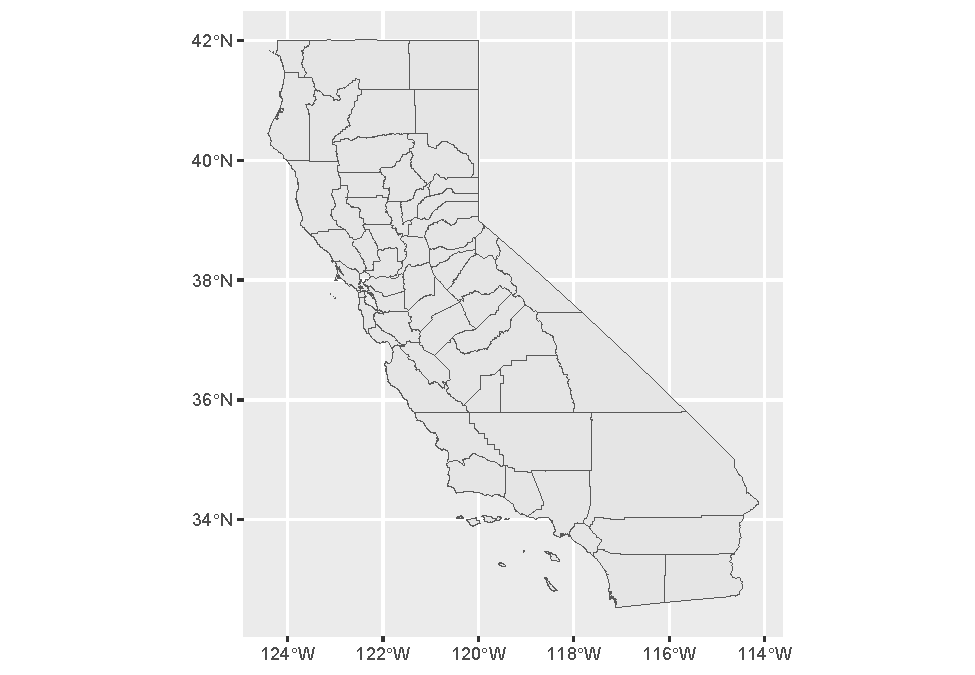
\includegraphics[width=0.75\linewidth]{EnvDataScience_files/figure-latex/mapsGGsimple-1} 

}

\caption{simple ggplot map}\label{fig:mapsGGsimple}
\end{figure}

Try \texttt{?geom\_sf} and you'll find that its first parameter is mapping with \texttt{aes()} by default. The data property is inherited from the ggplot call, but commonly you'll want to specify data=something in your geom\_sf call.

\textbf{Another simple ggplot, with labels}

Adding labels is also pretty easy using \texttt{aes()} (Figure \ref{fig:mapsGGlabels}).

\begin{Shaded}
\begin{Highlighting}[]
\FunctionTok{ggplot}\NormalTok{(CA\_counties) }\SpecialCharTok{+} \FunctionTok{geom\_sf}\NormalTok{() }\SpecialCharTok{+}
  \FunctionTok{geom\_sf\_text}\NormalTok{(}\FunctionTok{aes}\NormalTok{(}\AttributeTok{label =}\NormalTok{ NAME), }\AttributeTok{size =} \FloatTok{1.5}\NormalTok{)}
\end{Highlighting}
\end{Shaded}

\begin{figure}

{\centering 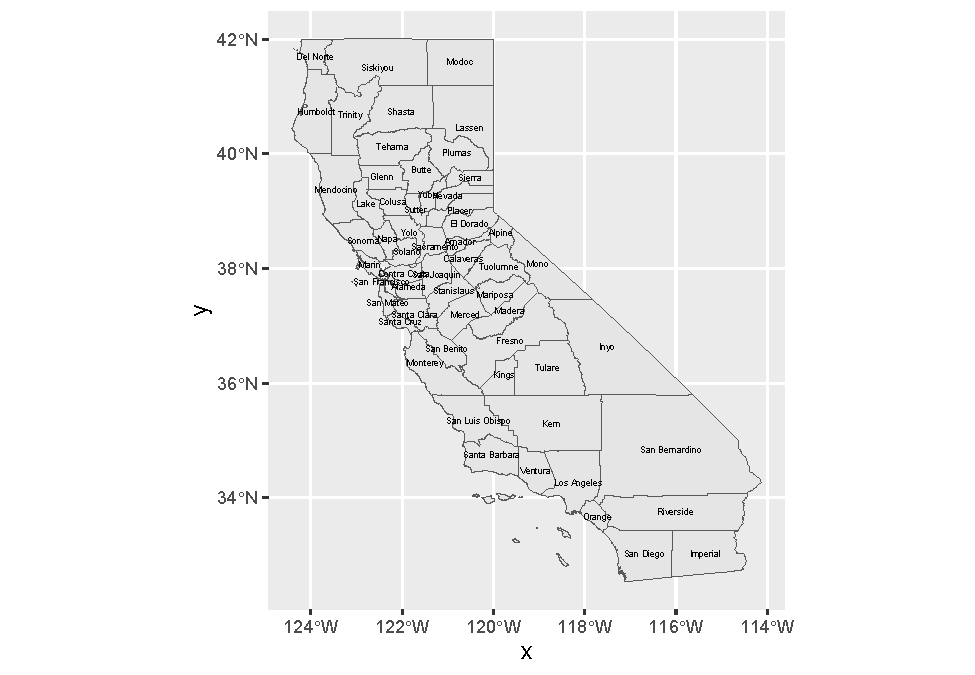
\includegraphics[width=0.75\linewidth]{EnvDataScience_files/figure-latex/mapsGGlabels-1} 

}

\caption{labels added}\label{fig:mapsGGlabels}
\end{figure}

\textbf{And now with fill color, repositioned legend, and no ``x'' or ``y'' labels}

The x and y labels are unnecessary since the graticule is provided, and for many maps there's a better place to put the legend than what happens by default -- for California's shape, the legend goes best in Nevada (Figure \ref{fig:mapsLegend}). We'll also pick a color scheme using \texttt{scale\_fill\_gradient} to specify the darkest color for high values, which corresponds to a cartographic figure-ground contrast rule.

\begin{Shaded}
\begin{Highlighting}[]
\FunctionTok{ggplot}\NormalTok{(CA\_counties) }\SpecialCharTok{+} \FunctionTok{geom\_sf}\NormalTok{(}\FunctionTok{aes}\NormalTok{(}\AttributeTok{fill=}\NormalTok{MED\_AGE)) }\SpecialCharTok{+}
  \FunctionTok{geom\_sf\_text}\NormalTok{(}\FunctionTok{aes}\NormalTok{(}\AttributeTok{label =}\NormalTok{ NAME), }\AttributeTok{col=}\StringTok{"white"}\NormalTok{, }\AttributeTok{size=}\FloatTok{1.5}\NormalTok{) }\SpecialCharTok{+}
  \FunctionTok{scale\_fill\_gradient}\NormalTok{(}\AttributeTok{high =} \StringTok{"darkslategray"}\NormalTok{,}\AttributeTok{low=} \StringTok{"darkslategray3"}\NormalTok{) }\SpecialCharTok{+}
  \FunctionTok{theme}\NormalTok{(}\AttributeTok{legend.position =} \FunctionTok{c}\NormalTok{(}\FloatTok{0.8}\NormalTok{, }\FloatTok{0.8}\NormalTok{)) }\SpecialCharTok{+}
  \FunctionTok{labs}\NormalTok{(}\AttributeTok{x=}\StringTok{""}\NormalTok{,}\AttributeTok{y=}\StringTok{""}\NormalTok{)}
\end{Highlighting}
\end{Shaded}

\begin{figure}

{\centering 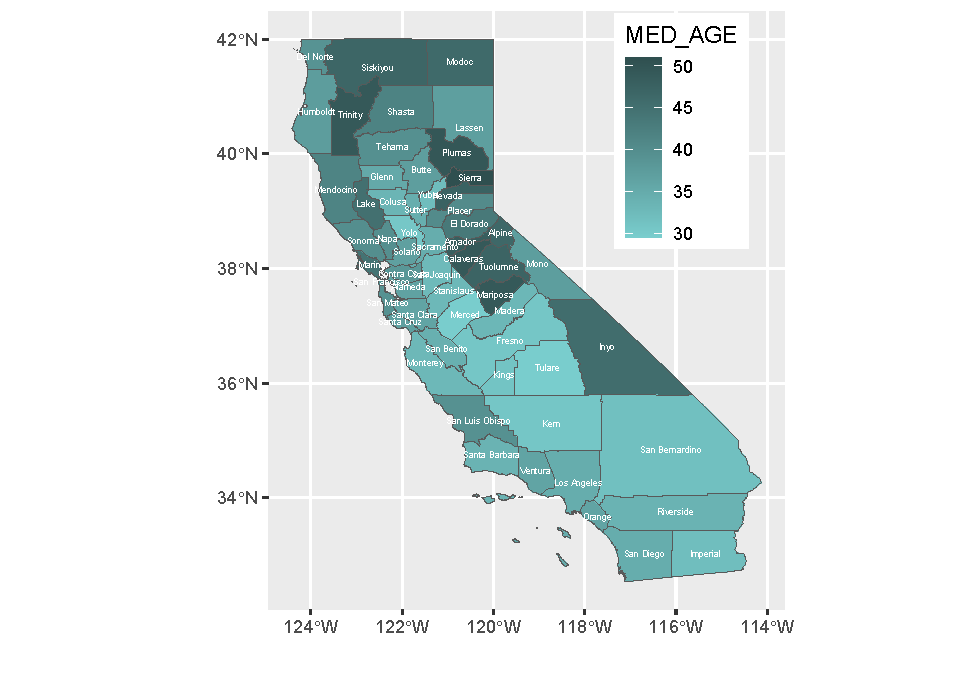
\includegraphics[width=0.75\linewidth]{EnvDataScience_files/figure-latex/mapsLegend-1} 

}

\caption{repositioned legend}\label{fig:mapsLegend}
\end{figure}

\textbf{Map in ggplot2, zoomed into two counties}

We can zoom into two counties by accessing the extent of an existing spatial dataset using \index{st\_bbox()}\texttt{st\_bbox()} \index{st\_make\_valid}(Figure \ref{fig:mapsZoom}).

\begin{Shaded}
\begin{Highlighting}[]
\FunctionTok{library}\NormalTok{(tidyverse); }\FunctionTok{library}\NormalTok{(sf); }\FunctionTok{library}\NormalTok{(igisci)}
\NormalTok{census }\OtherTok{\textless{}{-}} \FunctionTok{st\_make\_valid}\NormalTok{(BayAreaTracts) }\SpecialCharTok{\%\textgreater{}\%} \CommentTok{\#st\_make\_valid not needed ?}
   \FunctionTok{filter}\NormalTok{(CNTY\_FIPS }\SpecialCharTok{\%in\%} \FunctionTok{c}\NormalTok{(}\StringTok{"013"}\NormalTok{, }\StringTok{"095"}\NormalTok{))}
\NormalTok{TRI }\OtherTok{\textless{}{-}} \FunctionTok{read\_csv}\NormalTok{(}\FunctionTok{ex}\NormalTok{(}\StringTok{"TRI/TRI\_2017\_CA.csv"}\NormalTok{)) }\SpecialCharTok{\%\textgreater{}\%}
  \FunctionTok{st\_as\_sf}\NormalTok{(}\AttributeTok{coords =} \FunctionTok{c}\NormalTok{(}\StringTok{"LONGITUDE"}\NormalTok{, }\StringTok{"LATITUDE"}\NormalTok{), }\AttributeTok{crs=}\DecValTok{4326}\NormalTok{) }\SpecialCharTok{\%\textgreater{}\%}
  \FunctionTok{st\_join}\NormalTok{(census) }\SpecialCharTok{\%\textgreater{}\%}
  \FunctionTok{filter}\NormalTok{(CNTY\_FIPS }\SpecialCharTok{\%in\%} \FunctionTok{c}\NormalTok{(}\StringTok{"013"}\NormalTok{, }\StringTok{"095"}\NormalTok{),}
\NormalTok{         (}\StringTok{\textasciigrave{}}\AttributeTok{5.1\_FUGITIVE\_AIR}\StringTok{\textasciigrave{}} \SpecialCharTok{+} \StringTok{\textasciigrave{}}\AttributeTok{5.2\_STACK\_AIR}\StringTok{\textasciigrave{}}\NormalTok{) }\SpecialCharTok{\textgreater{}} \DecValTok{0}\NormalTok{)}
\NormalTok{bnd }\OtherTok{=} \FunctionTok{st\_bbox}\NormalTok{(census)}
\FunctionTok{ggplot}\NormalTok{() }\SpecialCharTok{+}
  \FunctionTok{geom\_sf}\NormalTok{(}\AttributeTok{data =}\NormalTok{ BayAreaCounties, }\FunctionTok{aes}\NormalTok{(}\AttributeTok{fill =}\NormalTok{ NAME)) }\SpecialCharTok{+}
  \FunctionTok{geom\_sf}\NormalTok{(}\AttributeTok{data =}\NormalTok{ census, }\AttributeTok{color=}\StringTok{"grey40"}\NormalTok{, }\AttributeTok{fill =} \ConstantTok{NA}\NormalTok{) }\SpecialCharTok{+}
  \FunctionTok{geom\_sf}\NormalTok{(}\AttributeTok{data =}\NormalTok{ TRI) }\SpecialCharTok{+}
  \FunctionTok{coord\_sf}\NormalTok{(}\AttributeTok{xlim =} \FunctionTok{c}\NormalTok{(bnd[}\DecValTok{1}\NormalTok{], bnd[}\DecValTok{3}\NormalTok{]), }\AttributeTok{ylim =} \FunctionTok{c}\NormalTok{(bnd[}\DecValTok{2}\NormalTok{], bnd[}\DecValTok{4}\NormalTok{])) }\SpecialCharTok{+}
  \FunctionTok{labs}\NormalTok{(}\AttributeTok{title=}\StringTok{"Census Tracts and TRI air{-}release sites"}\NormalTok{) }\SpecialCharTok{+}
  \FunctionTok{theme}\NormalTok{(}\AttributeTok{legend.position =} \StringTok{"none"}\NormalTok{)}
\end{Highlighting}
\end{Shaded}

\begin{figure}

{\centering 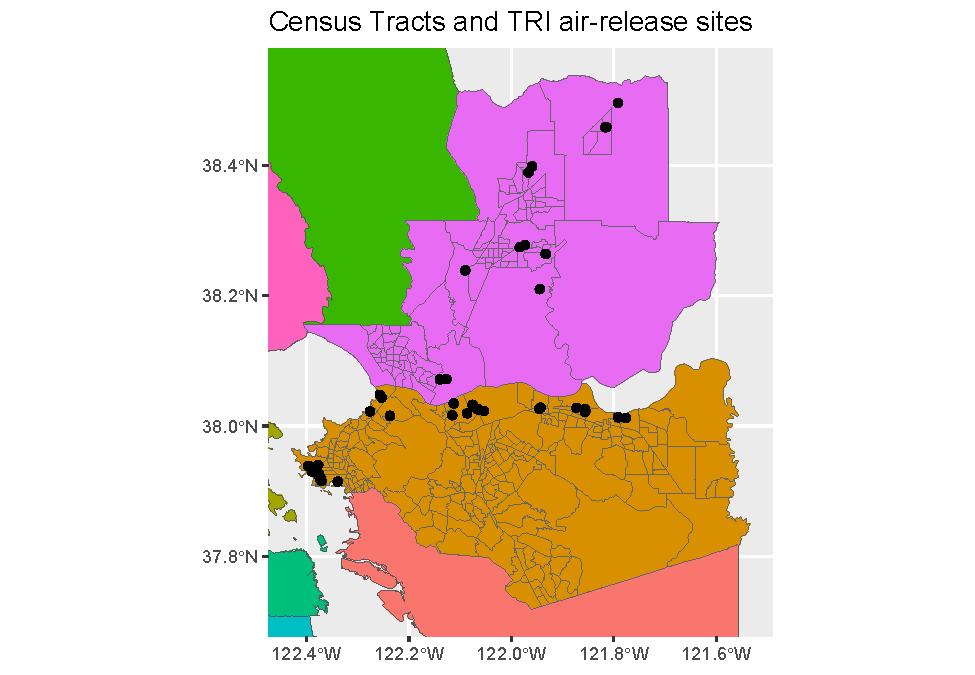
\includegraphics[width=0.75\linewidth]{EnvDataScience_files/figure-latex/mapsZoom-1} 

}

\caption{Using bbox to zoom into two counties}\label{fig:mapsZoom}
\end{figure}

\subsection{Rasters in ggplot2}\label{rasters-in-ggplot2}

\index{rasters in ggplot2}Raster display in \texttt{ggplot2} is currently a little awkward, as are rasters in general in the world of database-centric GIS where rasters don't comfortably sit.

We can use a trick: converting rasters to a grid of points, to then be able to create Figure \ref{fig:mapsGGrasters}.

\begin{Shaded}
\begin{Highlighting}[]
\FunctionTok{library}\NormalTok{(igisci)}
\FunctionTok{library}\NormalTok{(tidyverse)}
\FunctionTok{library}\NormalTok{(sf)}
\FunctionTok{library}\NormalTok{(terra)}
\NormalTok{elevation }\OtherTok{\textless{}{-}} \FunctionTok{rast}\NormalTok{(}\FunctionTok{ex}\NormalTok{(}\StringTok{"marbles/elev.tif"}\NormalTok{))}
\NormalTok{trails }\OtherTok{\textless{}{-}} \FunctionTok{st\_read}\NormalTok{(}\FunctionTok{ex}\NormalTok{(}\StringTok{"marbles/trails.shp"}\NormalTok{))}
\NormalTok{elevpts }\OtherTok{\textless{}{-}} \FunctionTok{st\_as\_sf}\NormalTok{(}\FunctionTok{as.points}\NormalTok{(elevation))}
\end{Highlighting}
\end{Shaded}

\begin{Shaded}
\begin{Highlighting}[]
\FunctionTok{ggplot}\NormalTok{() }\SpecialCharTok{+}
  \FunctionTok{geom\_sf}\NormalTok{(}\AttributeTok{data =}\NormalTok{ elevpts, }\FunctionTok{aes}\NormalTok{(}\AttributeTok{col=}\NormalTok{elev)) }\SpecialCharTok{+}
  \FunctionTok{geom\_sf}\NormalTok{(}\AttributeTok{data =}\NormalTok{ trails)}
\end{Highlighting}
\end{Shaded}

\begin{figure}

{\centering 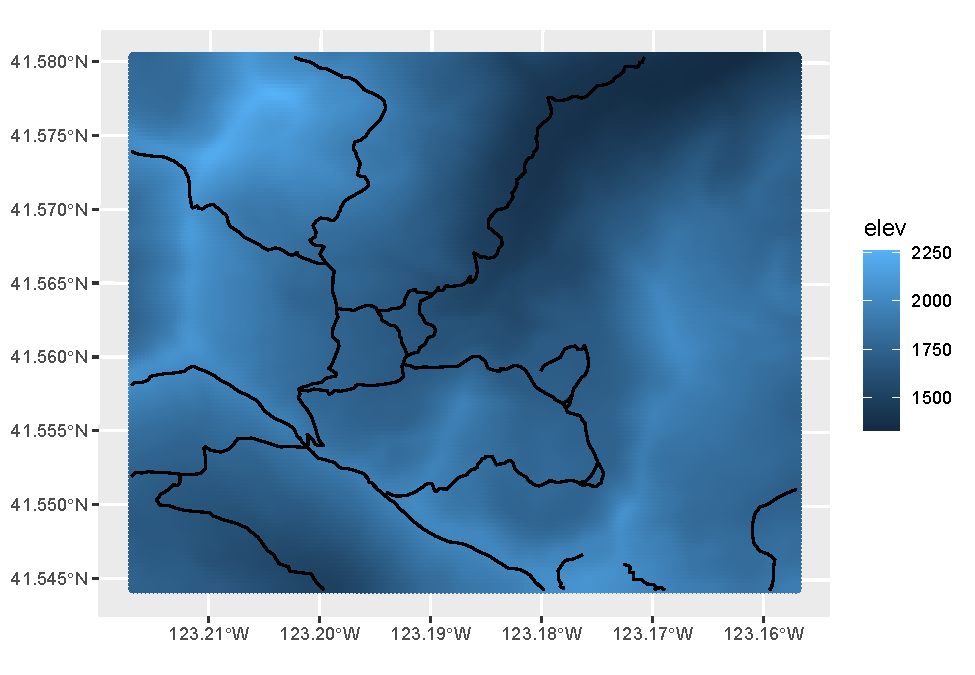
\includegraphics[width=0.75\linewidth]{EnvDataScience_files/figure-latex/mapsGGrasters-1} 

}

\caption{Rasters displayed in ggplot by converting to points}\label{fig:mapsGGrasters}
\end{figure}

Note that the raster name stored in the \texttt{elevation@pnt\$names} property is derived from the original source raster \texttt{elev.tif}, not from the object name we gave it, so we needed to specify \texttt{elev} for the variable to color from the resulting point features.

\begin{Shaded}
\begin{Highlighting}[]
\FunctionTok{names}\NormalTok{(elevation)}
\end{Highlighting}
\end{Shaded}

\begin{verbatim}
## [1] "elev"
\end{verbatim}

\section{Using bounding boxes to zoom to the extent of data layers (in any mapping package)}\label{using-bounding-boxes-to-zoom-to-the-extent-of-data-layers-in-any-mapping-package}

Bounding box functions like \texttt{st\_bbox} are important tools for zooming into the area of interest. Another one we'll use is \texttt{tmaptools::bb()}, thus part of the \texttt{tmaptools} package that is associated with the \texttt{tmap} mapping package we'll look at next.

\begin{Shaded}
\begin{Highlighting}[]
\FunctionTok{library}\NormalTok{(sf); }\FunctionTok{library}\NormalTok{(tmaptools); }\FunctionTok{library}\NormalTok{(igisci); }\FunctionTok{library}\NormalTok{(tidyverse)}
\NormalTok{trails }\OtherTok{\textless{}{-}} \FunctionTok{st\_read}\NormalTok{(}\FunctionTok{ex}\NormalTok{(}\StringTok{"marbles/trails.shp"}\NormalTok{))}
\NormalTok{bbTrails }\OtherTok{\textless{}{-}} \FunctionTok{bb}\NormalTok{(trails)}
\end{Highlighting}
\end{Shaded}

They produce the same thing \ldots{}

\begin{Shaded}
\begin{Highlighting}[]
\FunctionTok{identical}\NormalTok{(bbTrails, }\FunctionTok{st\_bbox}\NormalTok{(trails))}
\end{Highlighting}
\end{Shaded}

\begin{verbatim}
## [1] TRUE
\end{verbatim}

\ldots{} and both include the \texttt{crs} of the data set \ldots{}

\begin{Shaded}
\begin{Highlighting}[]
\FunctionTok{str}\NormalTok{(bbTrails)}
\end{Highlighting}
\end{Shaded}

\begin{verbatim}
##  'bbox' Named num [1:4] 481904 4599197 486902 4603200
##  - attr(*, "names")= chr [1:4] "xmin" "ymin" "xmax" "ymax"
##  - attr(*, "crs")=List of 2
##   ..$ input: chr "NAD83 / UTM zone 10N"
##   ..$ wkt  : chr "PROJCRS[\"NAD83 / UTM zone 10N\",\n    BASEGEOGCRS[\"NAD83\",\n        DATUM[\"North American Datum 1983\",\n  "| __truncated__
##   ..- attr(*, "class")= chr "crs"
\end{verbatim}

\ldots{} but currently there's at least one advantage of \texttt{tmaptools::bb()}: the \texttt{ext} parameter let's you add a bit to the extent to allow the map to have some extra border, with 1 being the default, and a 10\% increase being 1.1, etc. We'll see the effect in some later maps.

\begin{Shaded}
\begin{Highlighting}[]
\NormalTok{bbTrails}
\end{Highlighting}
\end{Shaded}

\begin{verbatim}
##      xmin      ymin      xmax      ymax 
##  481903.8 4599196.5  486901.9 4603200.0
\end{verbatim}

\begin{Shaded}
\begin{Highlighting}[]
\FunctionTok{bb}\NormalTok{(trails,}\AttributeTok{ext=}\FloatTok{1.1}\NormalTok{)}
\end{Highlighting}
\end{Shaded}

\begin{verbatim}
##      xmin      ymin      xmax      ymax 
##  481653.9 4598996.3  487151.8 4603400.2
\end{verbatim}

\section{tmap}\label{tmap}

\index{tmap}The tmap package provides some nice cartographic capabilities. I'm increasingly using it for creating maps. We'll learn some of its capabilities, but for more thorough coverage, see the ``Making maps with R'' section of \emph{Geocomputation with R} (Lovelace et al. (\citeproc{ref-Geocomputation}{2019})).

\begin{quote}
In addition to what we'll cover here, you should also see the chapter on Making Maps \url{https://r.geocompx.org/adv-map} in Lovelace, Nowosad and Muenchow (2025) \emph{Geocomputation with R}.
\end{quote}

The basic building block is \texttt{tm\_shape(}data\texttt{)} followed by various layer elements, such as \texttt{tm\_polygons()}. The \texttt{tm\_shape} function can work with either features or rasters.

\begin{Shaded}
\begin{Highlighting}[]
\FunctionTok{library}\NormalTok{(spData); }\FunctionTok{library}\NormalTok{(tmap)}
\FunctionTok{tmap\_mode}\NormalTok{(}\StringTok{"plot"}\NormalTok{)}
\FunctionTok{tm\_shape}\NormalTok{(world) }\SpecialCharTok{+} \FunctionTok{tm\_polygons}\NormalTok{()}
\end{Highlighting}
\end{Shaded}

But we'll make a better map (Figure \ref{fig:tmapWorld}) by inserting a graticule before filling the polygons, then use \texttt{tm\_layout} for some useful cartographic settings: make the background light blue and avoid excessive inner margins.\index{tm\_layout}\index{tmap inner margins}\index{tmap background color}

\begin{quote}
Note that the inner.margins are set close to zero. This makes a better looking border, without extra non-existing border stuff showing. Setting to zero would however create an error, at least with this bbox.
\end{quote}

\begin{Shaded}
\begin{Highlighting}[]
\FunctionTok{library}\NormalTok{(spData); }\FunctionTok{library}\NormalTok{(tmap); }\FunctionTok{library}\NormalTok{(sf)}
\NormalTok{bounds }\OtherTok{\textless{}{-}} \FunctionTok{st\_bbox}\NormalTok{(world)}
\NormalTok{marg }\OtherTok{\textless{}{-}} \FloatTok{0.0001}
\FunctionTok{tm\_graticules}\NormalTok{() }\SpecialCharTok{+}
  \FunctionTok{tm\_shape}\NormalTok{(world) }\SpecialCharTok{+} \FunctionTok{tm\_polygons}\NormalTok{() }\SpecialCharTok{+} \CommentTok{\# , bbox=bounds}
  \FunctionTok{tm\_layout}\NormalTok{(}\AttributeTok{bg.color=}\StringTok{"lightblue"}\NormalTok{, }\AttributeTok{inner.margins=}\NormalTok{marg)}
\end{Highlighting}
\end{Shaded}

\begin{figure}

{\centering 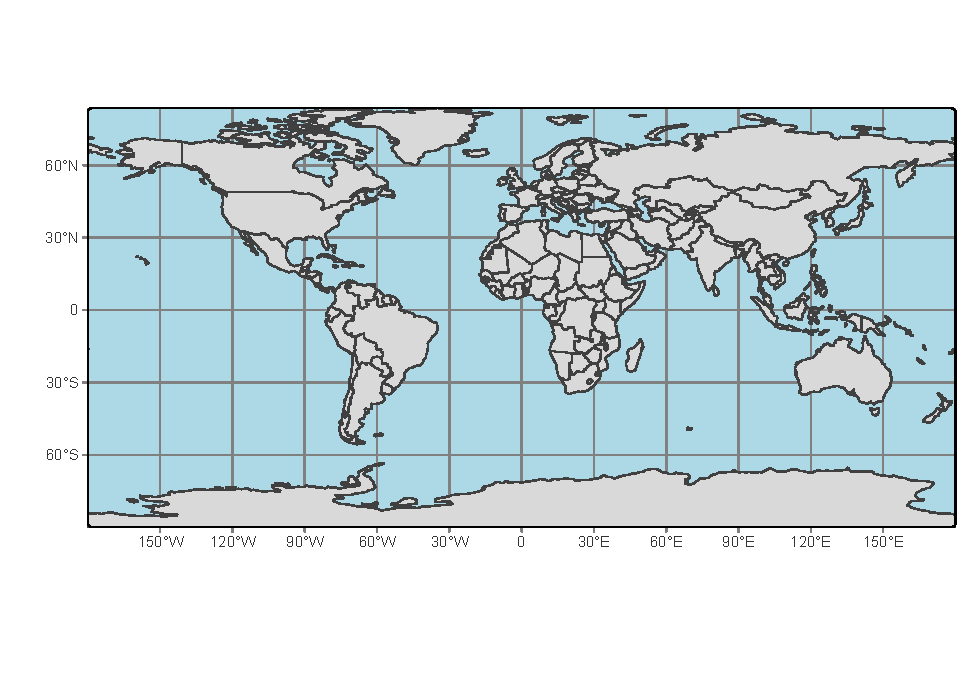
\includegraphics[width=0.75\linewidth]{EnvDataScience_files/figure-latex/tmapWorld-1} 

}

\caption{tmap with graticule}\label{fig:tmapWorld}
\end{figure}

\begin{quote}
Though it's not required, I like to start with \texttt{tm\_graticule}, then the first \texttt{tm\_shape} is indented, and then I follow that indentation standard, with each draw function (e.g.~\texttt{tm\_polygons}) applied to that shape either on the same line or indented further from the \texttt{tm\_shape}.
\end{quote}

\begin{quote}
Experiment by leaving settings out to see the effect, and explore other options with \texttt{?tm\_layout}, etc. The tmap package has a wealth of options, just a few of which we'll explore. For instance, we might want to use a different map projection than the default.
\end{quote}

\subsection{Color}\label{color}

As with plot and ggplot2, we can reference a variable to provide a range of colors for features we're plotting, such as coloring polygon fills (\texttt{tm\_fill} is a variant of \texttt{tm\_polygons} that only fills) to create a choropleth map (Figure \ref{fig:tmapColorVar}). In tmap, this is part of the concept of ``Visual variables''. We'll cover a bit about these, but see the ``Making maps with R'' chapter of \emph{Geocomputation with R} (\url{https://r.geocompx.org/}) for more on this and tmap in general.

Color scales are important to understand, and tmap4 makes use of colors in the c4a system, best seen by running \texttt{cols4all::c4a\_gui()}, which will run a Shiny app displaying the various options. \emph{Note that nothing else will run while this is in force, but you can also open in a browser.}

\begin{Shaded}
\begin{Highlighting}[]
\FunctionTok{library}\NormalTok{(sf); }\FunctionTok{library}\NormalTok{(igisci); }\FunctionTok{library}\NormalTok{(tmap)}
\FunctionTok{tm\_graticules}\NormalTok{(}\AttributeTok{col=}\StringTok{"gray95"}\NormalTok{) }\SpecialCharTok{+} \CommentTok{\# \#e5e7e9") +}
  \FunctionTok{tm\_shape}\NormalTok{(BayAreaTracts) }\SpecialCharTok{+}
    \FunctionTok{tm\_fill}\NormalTok{(}\AttributeTok{fill =} \StringTok{"MED\_AGE"}\NormalTok{, }\AttributeTok{fill.scale=}\FunctionTok{tm\_scale}\NormalTok{(}\AttributeTok{values=}\StringTok{"oranges"}\NormalTok{), }
            \AttributeTok{fill.legend=}\FunctionTok{tm\_legend}\NormalTok{(}\AttributeTok{position=}\FunctionTok{tm\_pos\_in}\NormalTok{(}\StringTok{"left"}\NormalTok{,}\StringTok{"bottom"}\NormalTok{),}
                                  \AttributeTok{bg.color=}\StringTok{"white"}\NormalTok{)) }\SpecialCharTok{+}
  \FunctionTok{tm\_shape}\NormalTok{(BayAreaCounties) }\SpecialCharTok{+}
    \FunctionTok{tm\_borders}\NormalTok{(}\AttributeTok{col\_alpha=}\FloatTok{0.2}\NormalTok{) }\SpecialCharTok{+}
  \FunctionTok{tm\_layout}\NormalTok{(}\AttributeTok{bg.color =} \StringTok{"gray90"}\NormalTok{)}
\end{Highlighting}
\end{Shaded}

\begin{figure}

{\centering 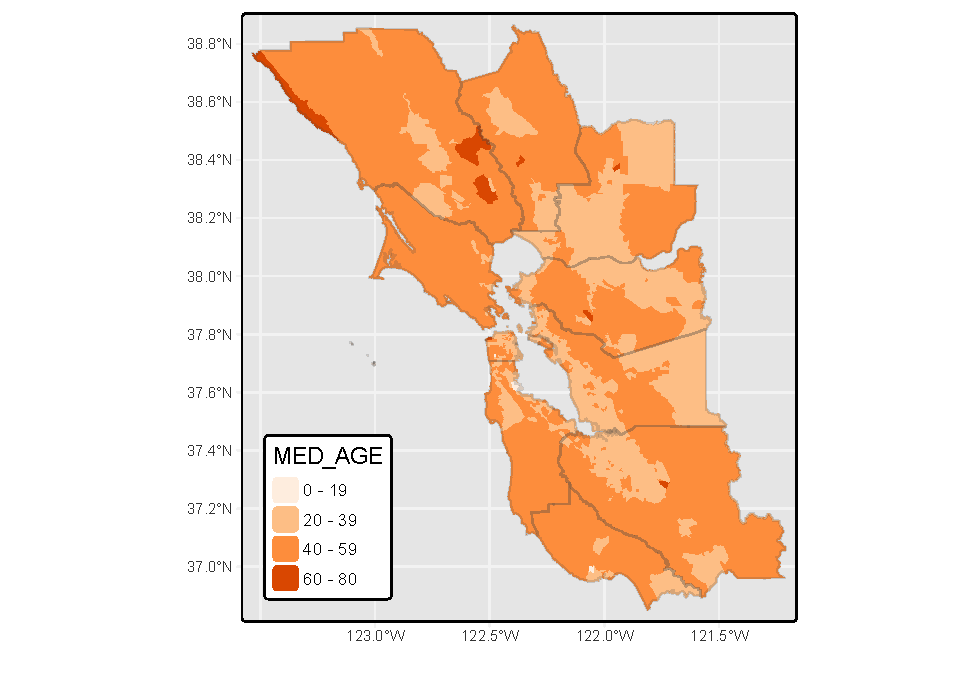
\includegraphics[width=0.75\linewidth]{EnvDataScience_files/figure-latex/tmapColorVar-1} 

}

\caption{tmap fill colored by variable}\label{fig:tmapColorVar}
\end{figure}

\begin{quote}
Note the legend formatting applied to position within the frame and the use of a background color. The continuous scale used here is from the \texttt{brewer} set, which you can explore at \texttt{cols4all::c4a\_gui()} by selecting the a sequential palette type and look through the \texttt{brewer} listings. They include single color ranges like ``greens'', ``purples'', ``blues'', etc., or ones that range from colors like yellow to green, like ``yl\_gn'', while still progressing from light to dark. We also used simple R colors.
\end{quote}

\textbf{Categorical Fill}

There are many choices of categorical color palettes you can explore using \texttt{cols4all::c4a\_gui()}, which allows you to set the number of colors you want and find many good options ranging from bold to subdued. For the 10-county greater Bay Area, the ``tableau.miller\_stone'' looks appealing, so we'll try it (\ref{fig:tmapCountyCategorical}). We'll also go without a frame for a legend placed outside.

\begin{Shaded}
\begin{Highlighting}[]
\FunctionTok{library}\NormalTok{(sf); }\FunctionTok{library}\NormalTok{(igisci); }\FunctionTok{library}\NormalTok{(tmap)}
\FunctionTok{tm\_graticules}\NormalTok{(}\AttributeTok{col=}\StringTok{"gray95"}\NormalTok{) }\SpecialCharTok{+} 
  \FunctionTok{tm\_shape}\NormalTok{(BayAreaCounties) }\SpecialCharTok{+} 
  \FunctionTok{tm\_polygons}\NormalTok{(}\AttributeTok{fill=}\StringTok{"NAME"}\NormalTok{, }
              \AttributeTok{fill.scale=}\FunctionTok{tm\_scale\_categorical}\NormalTok{(}\AttributeTok{values=}\StringTok{"tableau.miller\_stone"}\NormalTok{),}
              \AttributeTok{fill.legend=}\FunctionTok{tm\_legend}\NormalTok{(}\AttributeTok{frame=}\NormalTok{F,}\AttributeTok{title=}\StringTok{"County"}\NormalTok{)) }\SpecialCharTok{+}
  \FunctionTok{tm\_layout}\NormalTok{(}\AttributeTok{bg.color =} \StringTok{"gray90"}\NormalTok{)}
\end{Highlighting}
\end{Shaded}

\begin{figure}

{\centering 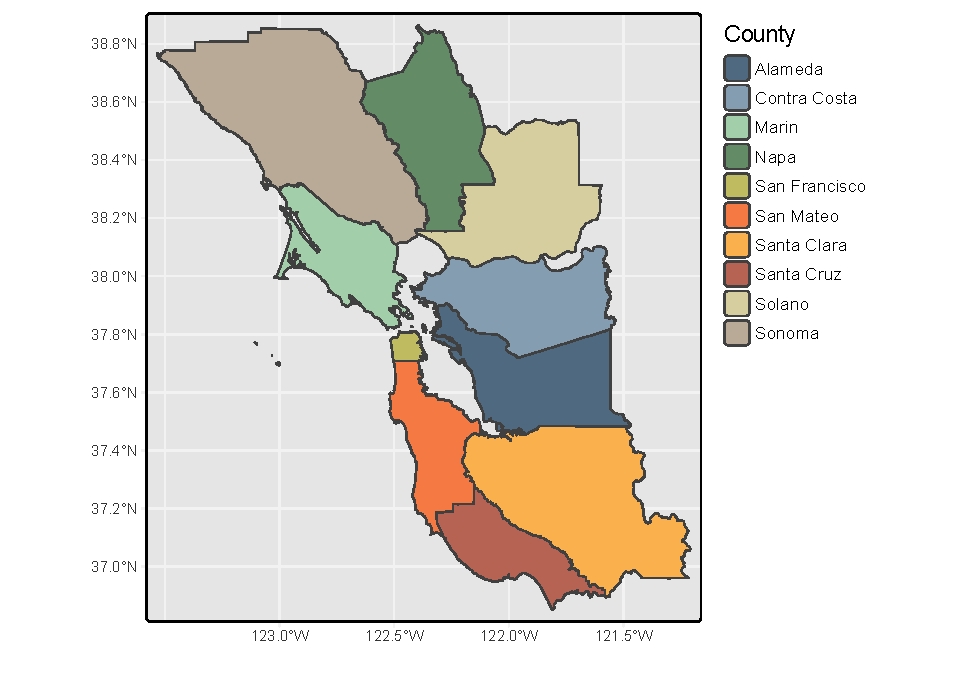
\includegraphics[width=0.75\linewidth]{EnvDataScience_files/figure-latex/tmapCountyCategorical-1} 

}

\caption{Categorical Fill}\label{fig:tmapCountyCategorical}
\end{figure}

\textbf{tmap of sierraFeb with hillshade and point symbols}

We'll use a raster hillshade as a basemap using \texttt{tm\_raster}, zoom into an area with a bounding box (using \texttt{tmaptools::bb}), include county boundaries with \texttt{tm\_borders}, and color station points with temperatures with \texttt{tm\_symbols} (Figure \ref{fig:tmapMulti}), with the legend positioned within the map frame.

\begin{Shaded}
\begin{Highlighting}[]
\FunctionTok{library}\NormalTok{(tmap); }\FunctionTok{library}\NormalTok{(sf); }\FunctionTok{library}\NormalTok{(terra); }\FunctionTok{library}\NormalTok{(igisci)}
\FunctionTok{library}\NormalTok{(tmaptools)}\CommentTok{\#; library(cols4all)}
\NormalTok{hillshCol }\OtherTok{\textless{}{-}} \FunctionTok{tm\_scale\_continuous}\NormalTok{(}\AttributeTok{values =} \StringTok{"{-}brewer.greys"}\NormalTok{)}
\end{Highlighting}
\end{Shaded}

\begin{Shaded}
\begin{Highlighting}[]
\FunctionTok{library}\NormalTok{(terra); }\FunctionTok{library}\NormalTok{(tidyverse)}
\FunctionTok{tmap\_mode}\NormalTok{(}\StringTok{"plot"}\NormalTok{)}
\NormalTok{sierra }\OtherTok{\textless{}{-}} \FunctionTok{st\_as\_sf}\NormalTok{(sierraFeb, }\AttributeTok{coords =} \FunctionTok{c}\NormalTok{(}\StringTok{"LONGITUDE"}\NormalTok{, }\StringTok{"LATITUDE"}\NormalTok{), }\AttributeTok{crs =} \DecValTok{4326}\NormalTok{) }\SpecialCharTok{|\textgreater{}}
  \FunctionTok{filter}\NormalTok{(}\SpecialCharTok{!}\FunctionTok{is.na}\NormalTok{(TEMPERATURE))}
\NormalTok{hillsh }\OtherTok{\textless{}{-}} \FunctionTok{rast}\NormalTok{(}\FunctionTok{ex}\NormalTok{(}\StringTok{"CA/ca\_hillsh\_WGS84.tif"}\NormalTok{))}
\NormalTok{ct }\OtherTok{\textless{}{-}} \FunctionTok{st\_read}\NormalTok{(}\FunctionTok{system.file}\NormalTok{(}\StringTok{"extdata"}\NormalTok{,}\StringTok{"sierra/CA\_places.shp"}\NormalTok{,}\AttributeTok{package=}\StringTok{"igisci"}\NormalTok{))}
\NormalTok{ct}\SpecialCharTok{$}\NormalTok{AREANAME\_pad }\OtherTok{\textless{}{-}} \FunctionTok{paste0}\NormalTok{(}\FunctionTok{str\_replace\_all}\NormalTok{(ct}\SpecialCharTok{$}\NormalTok{AREANAME,}\StringTok{\textquotesingle{}[A{-}Za{-}z]\textquotesingle{}}\NormalTok{,}\StringTok{\textquotesingle{} \textquotesingle{}}\NormalTok{),ct}\SpecialCharTok{$}\NormalTok{AREANAME)}
\NormalTok{tempScale }\OtherTok{\textless{}{-}} \FunctionTok{tm\_scale\_continuous}\NormalTok{(}\AttributeTok{values=}\StringTok{"{-}red\_blue\_diverging"}\NormalTok{,}\AttributeTok{midpoint=}\ConstantTok{NA}\NormalTok{)}
\NormalTok{hillsh }\OtherTok{\textless{}{-}} \FunctionTok{rast}\NormalTok{(}\FunctionTok{ex}\NormalTok{(}\StringTok{"CA/ca\_hillsh\_WGS84.tif"}\NormalTok{))}
\NormalTok{bounds }\OtherTok{\textless{}{-}} \FunctionTok{bb}\NormalTok{(sierra, }\AttributeTok{ext=}\FloatTok{1.1}\NormalTok{)}
\end{Highlighting}
\end{Shaded}

\begin{Shaded}
\begin{Highlighting}[]
\NormalTok{mapBase }\OtherTok{\textless{}{-}} \FunctionTok{tm\_graticules}\NormalTok{(}\AttributeTok{col=}\StringTok{"azure2"}\NormalTok{, }\AttributeTok{lines=}\NormalTok{T) }\SpecialCharTok{+}
  \FunctionTok{tm\_shape}\NormalTok{(hillsh, }\AttributeTok{bbox=}\NormalTok{bounds) }\SpecialCharTok{+} 
    \FunctionTok{tm\_raster}\NormalTok{(}\AttributeTok{col.scale=}\FunctionTok{tm\_scale\_continuous}\NormalTok{(}\AttributeTok{values=}\StringTok{"{-}brewer.greys"}\NormalTok{),}
              \AttributeTok{col.legend =} \FunctionTok{tm\_legend}\NormalTok{(}\AttributeTok{show=}\NormalTok{F),}
              \AttributeTok{col\_alpha=}\FloatTok{0.7}\NormalTok{) }\SpecialCharTok{+}
  \FunctionTok{tm\_shape}\NormalTok{(}\FunctionTok{st\_make\_valid}\NormalTok{(CA\_counties)) }\SpecialCharTok{+} \FunctionTok{tm\_borders}\NormalTok{() }\SpecialCharTok{+}
  \FunctionTok{tm\_shape}\NormalTok{(ct) }\SpecialCharTok{+} \FunctionTok{tm\_dots}\NormalTok{() }\SpecialCharTok{+} \FunctionTok{tm\_text}\NormalTok{(}\StringTok{"AREANAME"}\NormalTok{, }\AttributeTok{size=}\FloatTok{0.5}\NormalTok{)}
  
\NormalTok{mapBase }\SpecialCharTok{+}   
  \FunctionTok{tm\_shape}\NormalTok{(sierra) }\SpecialCharTok{+}
    \FunctionTok{tm\_symbols}\NormalTok{(}\AttributeTok{fill=}\StringTok{"TEMPERATURE"}\NormalTok{, }
               \AttributeTok{fill.scale=}\NormalTok{tempScale, }\AttributeTok{size=}\FloatTok{0.8}\NormalTok{,}
               \AttributeTok{fill.legend=}\FunctionTok{tm\_legend}\NormalTok{(}\StringTok{" C"}\NormalTok{,}\AttributeTok{reverse=}\NormalTok{T,}\AttributeTok{frame=}\NormalTok{F,}
                                     \AttributeTok{position=}\FunctionTok{tm\_pos\_in}\NormalTok{(}\StringTok{"right"}\NormalTok{,}\StringTok{"top"}\NormalTok{))) }\SpecialCharTok{+}
  \FunctionTok{tm\_title}\NormalTok{(}\StringTok{"February Normals"}\NormalTok{)}
\end{Highlighting}
\end{Shaded}

\begin{figure}

{\centering 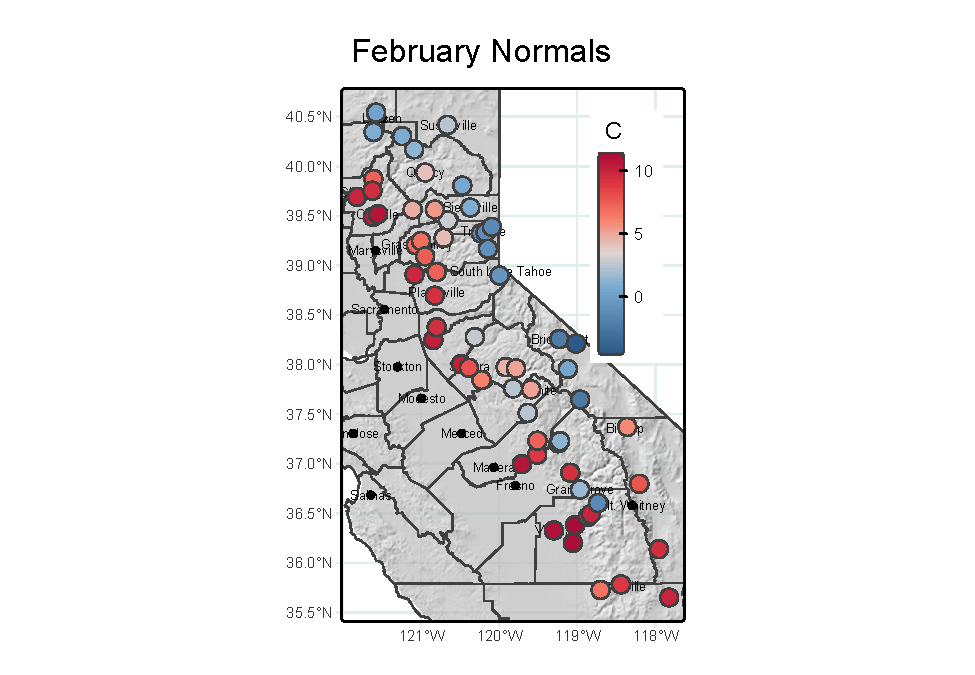
\includegraphics[width=0.75\linewidth]{EnvDataScience_files/figure-latex/tmapMulti-1} 

}

\caption{hillshade, borders and point symbols in tmap}\label{fig:tmapMulti}
\end{figure}

\begin{quote}
As introduced earlier, note the use of indentation I added for improving the readability of the code, with draw operations indented from the associated tm\_shape, and all of the fill options lined up.
\end{quote}

\subsection{Basemap with tmap}\label{basemap-with-tmap}

\index{basemap, rgb}In the example above, we created a hillshade basemap that used \texttt{tm\_raster} to display as shades of gray. We can also display a color (3-band rgb) image using \texttt{tm\_rgb}, including maps for tile basemap servers such as \texttt{OpenStreetMap} accessed with \texttt{maptiles::get\_tiles}.

But tmap also provides a bit easier way to access these basemap tiles, using \texttt{tm\_basemap}, such as with one of the basemaps served by Esri:

\texttt{tm\_basemap(server\ =\ "Esri.WorldTopoMap")}

Note that there are many basemaps served you might explore at \url{https://leaflet-extras.github.io/leaflet-providers/preview/index.html}. However, not all are supported by tm\_basemap, so they may end up blank. Unfortunately, the various USGS basemaps are currently not supported, but the Esri and Open basemaps are generally reliable.

\begin{itemize}
\tightlist
\item
  Esri.WorldTerrain
\item
  Esri.WorldShadedRelief
\item
  Esri.WorldImagery
\item
  Esri.WorldGrayCanvas
\item
  Esri.NatGeoWorldMap
\item
  Esri.OceanBasemap
\item
  OpenStreetMap
\item
  OpenTopoMap
\end{itemize}

Since tmap uses maptiles, you can also find a list of those supported using \texttt{?maptiles::get\_tiles} however some that are listed don't work at all zoom levels.

(Figure \ref{fig:tmapBasemapCAcounties})

\begin{Shaded}
\begin{Highlighting}[]
\FunctionTok{library}\NormalTok{(tmap); }\FunctionTok{library}\NormalTok{(maptiles); }\FunctionTok{library}\NormalTok{(igisci)}
\end{Highlighting}
\end{Shaded}

\begin{Shaded}
\begin{Highlighting}[]
\NormalTok{bounds}\OtherTok{=}\FunctionTok{bb}\NormalTok{(CA\_counties, }\AttributeTok{ext=}\FloatTok{1.05}\NormalTok{)}
\NormalTok{CA }\OtherTok{\textless{}{-}} \FunctionTok{tm\_basemap}\NormalTok{(}\StringTok{"Esri.WorldTerrain"}\NormalTok{) }\SpecialCharTok{+} 
      \FunctionTok{tm\_shape}\NormalTok{(CA\_counties) }\SpecialCharTok{+} \FunctionTok{tm\_borders}\NormalTok{(}\AttributeTok{lwd=}\DecValTok{1}\NormalTok{, }\AttributeTok{col=}\StringTok{"red"}\NormalTok{) }\SpecialCharTok{+}
      \FunctionTok{tm\_graticules}\NormalTok{(}\AttributeTok{lines=}\NormalTok{F,}\AttributeTok{labels.rot=}\FunctionTok{c}\NormalTok{(}\DecValTok{0}\NormalTok{,}\DecValTok{90}\NormalTok{)) }\SpecialCharTok{+}
      \FunctionTok{tm\_title}\NormalTok{(}\StringTok{"CA counties on basemap"}\NormalTok{)}
\NormalTok{CA}
\end{Highlighting}
\end{Shaded}

\begin{figure}

{\centering 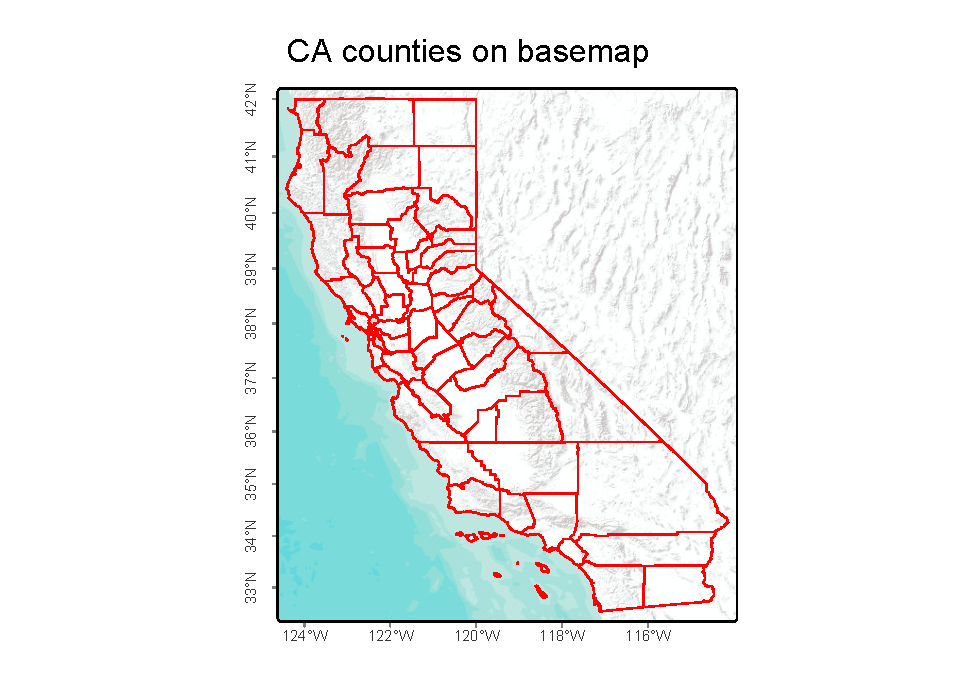
\includegraphics[width=0.75\linewidth]{EnvDataScience_files/figure-latex/tmapBasemapCAcounties-1} 

}

\caption{California counties with a basemap in tmap}\label{fig:tmapBasemapCAcounties}
\end{figure}

\begin{quote}
If you need labeled features for context, you can try some of the others, including the default OpenStreetMap, but you'll probably want to choose a specific zoom level that works, and that can be tricky. See \url{https://wiki.openstreetmap.org/wiki/Zoom_levels} for information on these; for instance \texttt{zoom=7} as an option for \texttt{get\_tiles} works pretty well for something at the scale of California.
\end{quote}

\section{Interactive Maps}\label{interactive-maps}

\index{interactive maps}The word ``static'' in ``static maps'' isn't something you would have heard in a cartography class thirty years ago, since essentially \emph{all} maps then were static. Very important in designing maps was, and still is, considering your audience and their perception of symbology.

\begin{itemize}
\tightlist
\item
  Figure-to-ground relationships assume ``ground'' is a white piece of paper (or possibly a standard white background in a pdf), so good cartographic color schemes tend to range from light for low values to dark for high values.
\item
  Scale is fixed, and there are no ``tools'' for changing scale, so a lot of attention must be paid to providing scale information.
\item
  Similarly, without the ability to see the map at different scales, inset maps are often needed to provide context.
\end{itemize}

While the purpose of static maps is to communicate information all at once, as a figure in a report or a printed poster, \emph{interactive} maps are about exploration, having tools for zooming in or out of an area of interest; they're also \emph{always} being ``printed'' on a computer or device where the color of the background isn't necessarily white. We are increasingly used to using interactive maps on our phones or other devices, where we're typically in exploratory mode, and often get frustrated not being able to zoom into a static map. However, as we'll see, there are trade-offs in that interactive maps don't provide the same level of control on symbology for what we want to put on the map, but instead depend a lot on basemaps for much of the cartographic design, generally limiting the symbology of data being mapped on top of it.

\begin{quote}
Earlier we looked at static tables where we might optimize the look of the table using tools like \texttt{gt::gt}. These are analogous to a static map, and for a more exploratory purpose we might instead display a data frame using a tool like \texttt{DT::datatable} that allows interactive methods such as scrolling.
\end{quote}

\subsection{Leaflet}\label{leaflet}

\index{leaflet}We'll come back to tmap to look at its interactive option, but we should start with a very brief look at the package that it uses when you choose interactive mode: \textbf{leaflet}. The R leaflet library itself translates to \emph{Javascript} and its \textbf{Leaflet} library, which was designed to support ``mobile-friendly interactive maps'' (\url{https://leafletjs.com}). We'll also look at another R package that translates to leaflet: \textbf{mapview}.

Interactive maps tend to focus on using basemaps for most of the cartographic design work, and quite a few are available. The only code required to display the basemap is \texttt{addTiles()}, which will display the default \texttt{OpenStreetMap} in the area where you provide any features, typically with \texttt{addMarkers()}. This default basemap is pretty good to use for general purposes, especially in urban areas where OpenStreetMap contributors (including a lot of former students I think) have provided a lot of data.

You can specify additional choices using \texttt{addProviderTiles()}, and use a layers control with the choices provided as \texttt{baseGroups}. You have access to all of the basemap provider names with the vector \texttt{providers}, and to see what they look like in your area, explore \url{http://leaflet-extras.github.io/leaflet-providers/preview/index.html}, where you can zoom into an area of interest and select the base map to see how it would look in a given zoom (Figure \ref{fig:mapsLeafletSFSU}).

\begin{Shaded}
\begin{Highlighting}[]
\FunctionTok{library}\NormalTok{(leaflet)}
\FunctionTok{leaflet}\NormalTok{() }\SpecialCharTok{\%\textgreater{}\%}
  \FunctionTok{addTiles}\NormalTok{(}\AttributeTok{group=}\StringTok{"OpenStreetMap"}\NormalTok{) }\SpecialCharTok{\%\textgreater{}\%}
  \FunctionTok{addProviderTiles}\NormalTok{(}\StringTok{"OpenTopoMap"}\NormalTok{,}\AttributeTok{group=}\StringTok{"OpenTopoMap"}\NormalTok{) }\SpecialCharTok{\%\textgreater{}\%}
  \FunctionTok{addProviderTiles}\NormalTok{(}\StringTok{"Esri.NatGeoWorldMap"}\NormalTok{,}\AttributeTok{group=}\StringTok{"Esri.NatGeoWorldMap"}\NormalTok{) }\SpecialCharTok{\%\textgreater{}\%}
  \FunctionTok{addProviderTiles}\NormalTok{(}\StringTok{"Esri.WorldImagery"}\NormalTok{,}\AttributeTok{group=}\StringTok{"Esri.WorldImagery"}\NormalTok{) }\SpecialCharTok{\%\textgreater{}\%}
  \FunctionTok{addMarkers}\NormalTok{(}\AttributeTok{lng=}\SpecialCharTok{{-}}\FloatTok{122.4756}\NormalTok{, }\AttributeTok{lat=}\FloatTok{37.72222}\NormalTok{,}
             \AttributeTok{popup=}\StringTok{"Institute for Geographic Information Science, SFSU"}\NormalTok{) }\SpecialCharTok{\%\textgreater{}\%}
  \FunctionTok{addLayersControl}\NormalTok{(}
    \AttributeTok{baseGroups =} \FunctionTok{c}\NormalTok{(}\StringTok{"OpenStreetMap"}\NormalTok{,}\StringTok{"OpenTopoMap"}\NormalTok{,}
                   \StringTok{"Esri.WorldImagery"}\NormalTok{,}\StringTok{"Esri.NatGeoWorldMap"}\NormalTok{))}
\end{Highlighting}
\end{Shaded}

\begin{figure}

{\centering 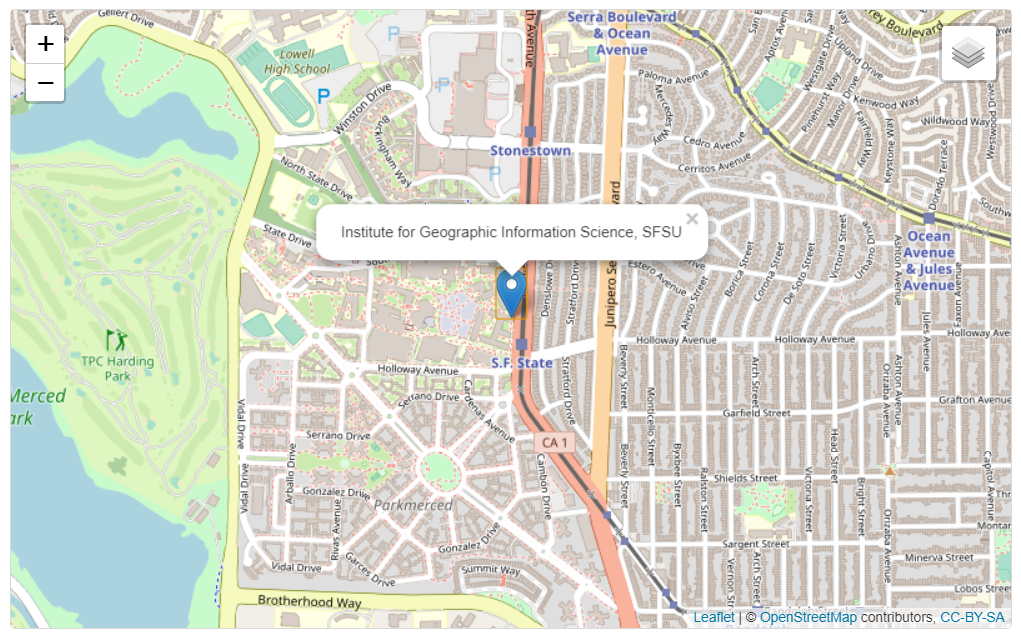
\includegraphics[width=0.75\linewidth]{img/mapLeafletSFSU} 

}

\caption{Leaflet map showing the location of the SFSU Institute for Geographic Information Science with choices of basemaps}\label{fig:mapsLeafletSFSU}
\end{figure}

With an interactive map, we do have the advantage of a good choice of base maps and the ability to resize and explore the map, but symbology is more limited, mostly just color and size, with only one variable in a legend. Note that interactive maps display in the Viewer window of RStudio or in R Markdown code output as you see in the html version of this book.

For a lot more information on the leaflet package in R, see:

\begin{itemize}
\tightlist
\item
  \url{https://blog.rstudio.com/2015/06/24/leaflet-interactive-web-maps-with-r/}
\item
  \url{https://github.com/rstudio/cheatsheets/blob/master/leaflet.pdf}
\end{itemize}

\subsection{Mapview}\label{mapview}

\index{mapview}In the \textbf{mapview} package, either \texttt{mapview} or \texttt{mapView} produces perhaps the simplest interactive map display where the view provides the option of changing basemaps, and just a couple of options make it a pretty useful system for visualizing point data. So for environmental work involving samples, it is a pretty useful exploratory tool.

\begin{Shaded}
\begin{Highlighting}[]
\FunctionTok{library}\NormalTok{(sf); }\FunctionTok{library}\NormalTok{(mapview)}
\NormalTok{sierra }\OtherTok{\textless{}{-}} \FunctionTok{st\_as\_sf}\NormalTok{(sierraFeb, }\AttributeTok{coords =} \FunctionTok{c}\NormalTok{(}\StringTok{"LONGITUDE"}\NormalTok{, }\StringTok{"LATITUDE"}\NormalTok{), }\AttributeTok{crs =} \DecValTok{4326}\NormalTok{)}
\FunctionTok{mapview}\NormalTok{(sierra, }\AttributeTok{zcol=}\StringTok{"TEMPERATURE"}\NormalTok{, }\AttributeTok{popup =} \ConstantTok{TRUE}\NormalTok{)}
\end{Highlighting}
\end{Shaded}

\begin{center}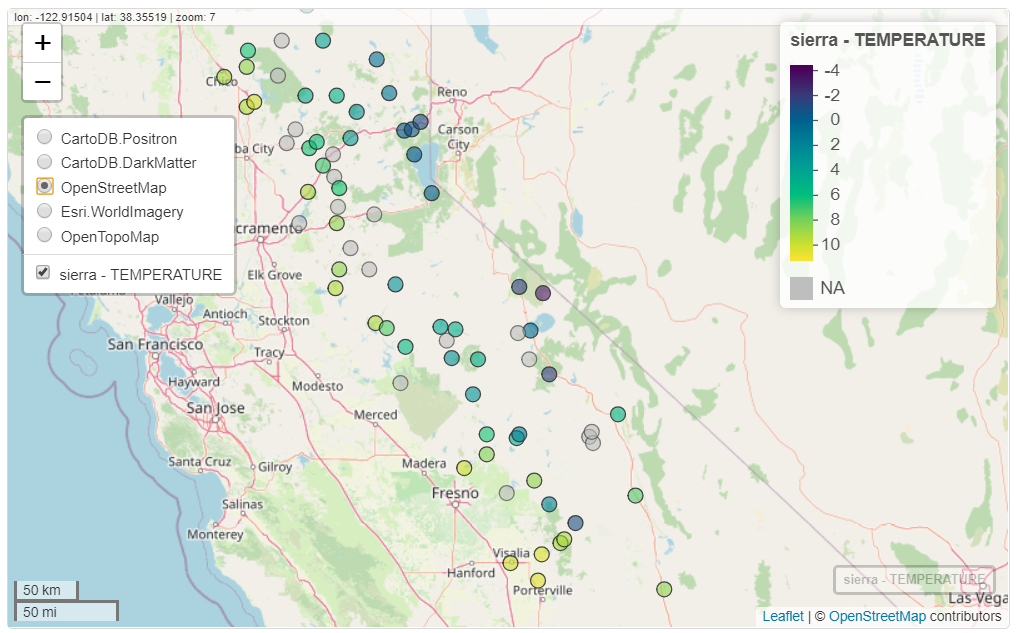
\includegraphics[width=0.75\linewidth]{img/mapview} \end{center}

\subsection{tmap (view mode)}\label{tmap-view-mode}

\index{tmap interactive view mode}You can change to an interactive mode with tmap by using \texttt{tmap\_mode("view")} so you might think that you can do all the great things that \texttt{tmap} does in normal plot mode here, but as we've seen, interactive maps don't provide the same level of symbology. The view mode of tmap, like mapview, is just a wrapper around leaflet, so we'll focus on the latter. The key parameter needed is \texttt{tmap\_mode}, which must be set to \texttt{"view"} to create an interactive map.

\begin{Shaded}
\begin{Highlighting}[]
\FunctionTok{library}\NormalTok{(tmap); }\FunctionTok{library}\NormalTok{(sf); }\FunctionTok{library}\NormalTok{(tmaptools); }\FunctionTok{library}\NormalTok{(tidyverse)}
\FunctionTok{tmap\_mode}\NormalTok{(}\StringTok{"view"}\NormalTok{)}
\NormalTok{sierra }\OtherTok{\textless{}{-}} \FunctionTok{st\_as\_sf}\NormalTok{(sierraFeb, }\AttributeTok{coords =} \FunctionTok{c}\NormalTok{(}\StringTok{"LONGITUDE"}\NormalTok{, }\StringTok{"LATITUDE"}\NormalTok{), }\AttributeTok{crs =} \DecValTok{4326}\NormalTok{) }\SpecialCharTok{|\textgreater{}}
  \FunctionTok{filter}\NormalTok{(}\SpecialCharTok{!}\FunctionTok{is.na}\NormalTok{(TEMPERATURE))}
\NormalTok{bounds }\OtherTok{\textless{}{-}} \FunctionTok{bb}\NormalTok{(sierra, }\AttributeTok{ext=}\FloatTok{1.1}\NormalTok{)}
\NormalTok{tempCol }\OtherTok{\textless{}{-}} \FunctionTok{tm\_scale\_continuous}\NormalTok{(}\AttributeTok{values =} \StringTok{"{-}brewer.RdBu"}\NormalTok{)}
\end{Highlighting}
\end{Shaded}

\begin{Shaded}
\begin{Highlighting}[]
\NormalTok{sierraMap }\OtherTok{\textless{}{-}} \FunctionTok{tm\_basemap}\NormalTok{(leaflet}\SpecialCharTok{::}\NormalTok{providers}\SpecialCharTok{$}\NormalTok{Esri.NatGeoWorldMap) }\SpecialCharTok{+}
  \FunctionTok{tm\_shape}\NormalTok{(sierra) }\SpecialCharTok{+} 
    \FunctionTok{tm\_dots}\NormalTok{(}\AttributeTok{fill=}\StringTok{"TEMPERATURE"}\NormalTok{,}
            \AttributeTok{fill.scale=}\NormalTok{tempCol,}
            \AttributeTok{fill.legend=}\FunctionTok{tm\_legend}\NormalTok{(}\AttributeTok{position=}\FunctionTok{tm\_pos\_in}\NormalTok{(}\StringTok{"right"}\NormalTok{,}\StringTok{"top"}\NormalTok{)),}
            \AttributeTok{fill\_alpha =} \FloatTok{0.66}\NormalTok{,}
            \AttributeTok{size=}\FloatTok{0.5}\NormalTok{)}
\FunctionTok{tmap\_leaflet}\NormalTok{(sierraMap, }\AttributeTok{show=}\ConstantTok{TRUE}\NormalTok{)}
\end{Highlighting}
\end{Shaded}

One nice feature of tmap view mode (and mapview) is the ability to select the basemap interactively using the layers symbol. There are lots of basemap available with leaflet (and thus with tmap view). To explore them, see \url{http://leaflet-extras.github.io/leaflet-providers/preview/index.html} but recognize that not all of these will work everywhere; many are highly localized or may only work at certain scales.

The following map using tmap could presumably be coded in leaflet, but tmap makes it a lot easier. We'll use it to demonstrate picking the basemap, which really can help in communicating our data with context (Figure \ref{fig:tmapBaseMaps}).

\begin{Shaded}
\begin{Highlighting}[]
\FunctionTok{library}\NormalTok{(sf); }\FunctionTok{library}\NormalTok{(tmap); }\FunctionTok{library}\NormalTok{(igisci); }\FunctionTok{library}\NormalTok{(tidyverse)}
\NormalTok{soilCO2 }\OtherTok{\textless{}{-}} \FunctionTok{st\_read}\NormalTok{(}\FunctionTok{ex}\NormalTok{(}\StringTok{"marbles/co2july95.shp"}\NormalTok{))}
\NormalTok{geology }\OtherTok{\textless{}{-}} \FunctionTok{st\_read}\NormalTok{(}\FunctionTok{ex}\NormalTok{(}\StringTok{"marbles/geology.shp"}\NormalTok{)) }\SpecialCharTok{|\textgreater{}} \FunctionTok{rename}\NormalTok{(}\AttributeTok{Geology=}\NormalTok{CLASS)}
\end{Highlighting}
\end{Shaded}

\begin{Shaded}
\begin{Highlighting}[]
\NormalTok{    tmap\_mode }\OtherTok{=} \StringTok{"view"}
\NormalTok{    map }\OtherTok{\textless{}{-}} \FunctionTok{tm\_basemap}\NormalTok{(}\AttributeTok{server=}\FunctionTok{c}\NormalTok{(}\AttributeTok{Topo=}\StringTok{"OpenTopoMap"}\NormalTok{,}
                      \AttributeTok{NatGeo=}\StringTok{"Esri.NatGeoWorldMap"}\NormalTok{,}
                      \AttributeTok{Imagery =} \StringTok{"Esri.WorldImagery"}\NormalTok{)) }\SpecialCharTok{+}
           \FunctionTok{tm\_shape}\NormalTok{(geology) }\SpecialCharTok{+}
              \FunctionTok{tm\_polygons}\NormalTok{(}\AttributeTok{fill=}\StringTok{"Geology"}\NormalTok{, }\AttributeTok{fill\_alpha=}\FloatTok{0.5}\NormalTok{) }\SpecialCharTok{+}
           \FunctionTok{tm\_shape}\NormalTok{(soilCO2) }\SpecialCharTok{+} 
              \FunctionTok{tm\_symbols}\NormalTok{(}\AttributeTok{fill=}\StringTok{"CO2\_"}\NormalTok{,}
                 \AttributeTok{fill.scale =} \FunctionTok{tm\_scale\_continuous}\NormalTok{())}
    \FunctionTok{tmap\_leaflet}\NormalTok{(map,}\AttributeTok{show=}\ConstantTok{TRUE}\NormalTok{)}
\end{Highlighting}
\end{Shaded}

\begin{figure}

{\centering 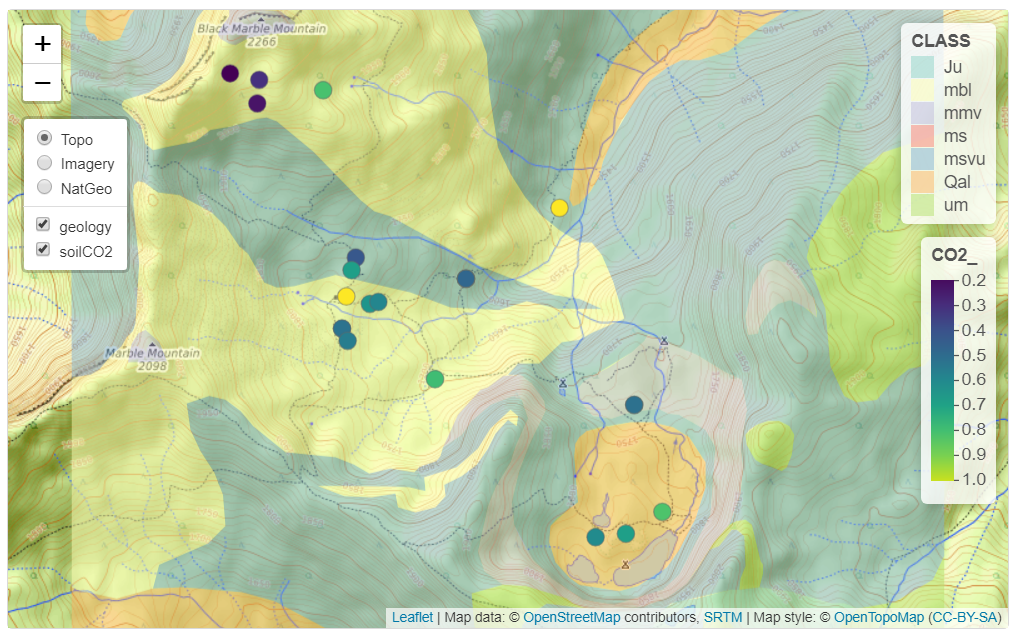
\includegraphics[width=0.75\linewidth]{img/tMapBaseMaps} 

}

\caption{View (interactive) mode of tmap with selection of basemaps}\label{fig:tmapBaseMaps}
\end{figure}

\subsection{Interactive mapping of individual penguins abstracted from a big dataset}\label{interactive-mapping-of-individual-penguins-abstracted-from-a-big-dataset}

\index{big data abstraction}In a study of spatial foraging patterns by Adélie penguins (\emph{Pygoscelis adeliae}), Ballard et al. (\citeproc{ref-Ballard2019}{2019}) collected data over five austral summer seasons (parts of December and January in 2005-06, 2006-07, 2007-08, 2008-09, 2012-13) period using SPLASH tags that combine Argos satellite tracking with a time-depth recorder, with 11,192 observations. The 24 SPLASH tags were re-used over the period of the project with a total of 162 individual breeding penguins, each active over a single season.

Our code takes advantage of the abstraction capabilities of base R and \texttt{dplyr} to select an individual penguin from the large data set and prepare its variables for useful display. Then the interactive mode of tmap works well for visualizing the penguin data -- both the cloud of all observations and the focused individual -- since we can zoom in to see the locations in context, and basemaps can be chosen. The \texttt{tmap} code colors the individual penguin's locations based on a decimal day derived from day and time. While interactive view is more limited in options, it does at least support a legend and title (Figure \ref{fig:mapsPenguins}).

\begin{Shaded}
\begin{Highlighting}[]
\FunctionTok{set.seed}\NormalTok{(}\DecValTok{28}\NormalTok{)}
\end{Highlighting}
\end{Shaded}

\begin{Shaded}
\begin{Highlighting}[]
\FunctionTok{library}\NormalTok{(sf); }\FunctionTok{library}\NormalTok{(tmap); }\FunctionTok{library}\NormalTok{(tidyverse); }\FunctionTok{library}\NormalTok{(igisci);}
\NormalTok{sat\_table }\OtherTok{\textless{}{-}} \FunctionTok{read\_csv}\NormalTok{(}\FunctionTok{ex}\NormalTok{(}\StringTok{"penguins/sat\_table\_splash.csv"}\NormalTok{))}
\NormalTok{obs }\OtherTok{\textless{}{-}} \FunctionTok{st\_as\_sf}\NormalTok{(}\FunctionTok{filter}\NormalTok{(sat\_table,include}\SpecialCharTok{==}\DecValTok{1}\NormalTok{), }\AttributeTok{coords=}\FunctionTok{c}\NormalTok{(}\StringTok{"lon"}\NormalTok{,}\StringTok{"lat"}\NormalTok{), }\AttributeTok{crs=}\DecValTok{4326}\NormalTok{)}
\NormalTok{uniq\_ids }\OtherTok{\textless{}{-}} \FunctionTok{unique}\NormalTok{(obs}\SpecialCharTok{$}\NormalTok{uniq\_id) }\CommentTok{\# uniq\_id identifies an individual penguin}
\NormalTok{onebird }\OtherTok{\textless{}{-}}\NormalTok{ obs }\SpecialCharTok{\%\textgreater{}\%}
  \FunctionTok{filter}\NormalTok{(uniq\_id}\SpecialCharTok{==}\NormalTok{uniq\_ids[}\FunctionTok{sample.int}\NormalTok{(}\FunctionTok{length}\NormalTok{(uniq\_ids), }\AttributeTok{size=}\DecValTok{1}\NormalTok{)]) }\SpecialCharTok{\%\textgreater{}\%}
  \FunctionTok{mutate}\NormalTok{(}\AttributeTok{decimalDay =} \FunctionTok{as.numeric}\NormalTok{(day) }\SpecialCharTok{+} \FunctionTok{as.numeric}\NormalTok{(hour)}\SpecialCharTok{/}\DecValTok{24}\NormalTok{)}
\NormalTok{tmap\_mode }\OtherTok{=} \StringTok{"view"}
\end{Highlighting}
\end{Shaded}

\begin{figure}

{\centering 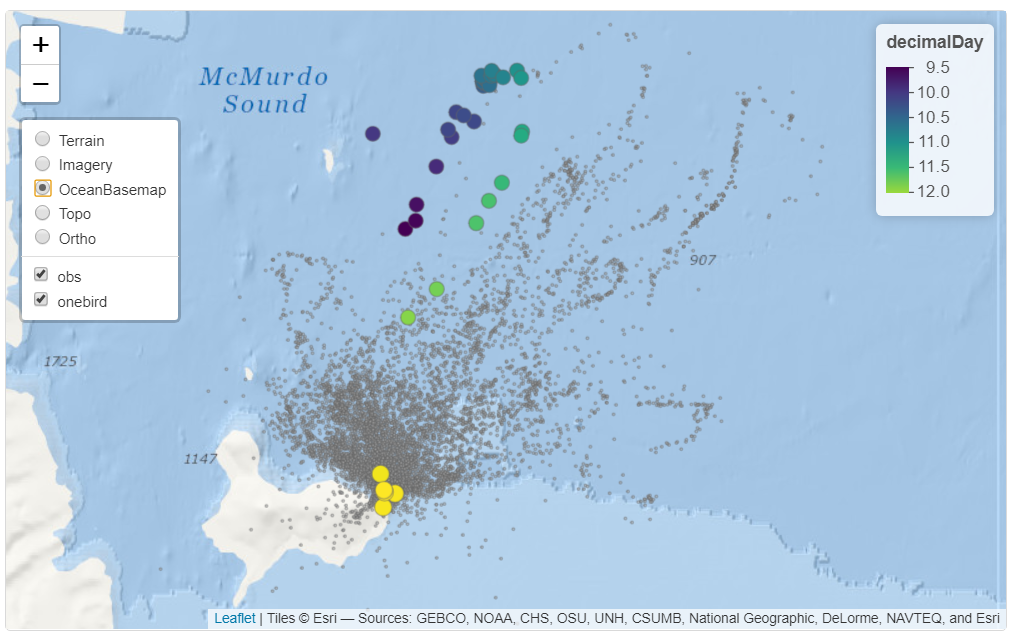
\includegraphics[width=0.75\linewidth]{img/mapsPenguins} 

}

\caption{Observations of Adélie penguin migration from a 5-season study of a large colony at Ross Island in the SW Ross Sea, Antarctica; and an individual -- H36CROZ0708 -- from season 0708. Data source: Ballard et al. (2019). Fine-scale oceanographic features characterizing successful Adélie penguin foraging in the SW Ross Sea. Marine Ecology Progress Series 608:263-277.}\label{fig:mapsPenguins}
\end{figure}

\begin{quote}
\textbf{Some final thoughts on maps and plotting/viewing packages}: There's a lot more to creating maps from spatial data, but we need to look at spatial analysis to create some products that we might want to create maps from. In the next chapter, in addition to looking at spatial analysis methods we'll also continue our exploration of map design, ranging from very simple exploratory outputs to more carefully designed products for sharing with others.
\end{quote}

\pagebreak

\section{Exercises: Spatial Data and Maps}\label{exercises-spatial-data-and-maps}

\textbf{Project preparation}: Create a new RStudio project, and name it ``Spatial''. We're going to use this for data we create and new data we want to bring in. We'll still be reading in data from the data package, but working in this project we'll be getting used to (a) working with our own data and (b) storing data to be used for later projects. Once we've created the project, we'll want to create a \texttt{data} folder to store data in. This code should do this:

\begin{Shaded}
\begin{Highlighting}[]
\NormalTok{dirname }\OtherTok{\textless{}{-}} \StringTok{"data"}
\ControlFlowTok{if}\NormalTok{ (}\SpecialCharTok{!}\FunctionTok{dir.exists}\NormalTok{(dirname)) \{}
  \FunctionTok{dir.create}\NormalTok{(dirname)}
\NormalTok{\}}
\end{Highlighting}
\end{Shaded}

\begin{exercise}
Using the method of building simple sf geometries, build a simple \(1\times1\) square object and plot it. Remember that you have to close the polygon, so the first vertex is the same as the last (of 5) vertices.
\end{exercise}

\begin{exercise}

Build a map in ggplot of Colorado, Wyoming, and Utah with these boundary vertices in GCS. As with the square, remember to close each figure, and assign the crs to what is needed for GCS: 4326.

\begin{itemize}
\tightlist
\item
  Colorado: (-109,41),(-102,41),(-102,37),(-109,37)
\item
  Wyoming: (-111,45),(-104,45),(-104,41),(-111,41)
\item
  Utah: (-114,42),(-111,42),(-111,41),(-109,41),(-109,37),(-114,37)
\end{itemize}

\end{exercise}

\begin{center}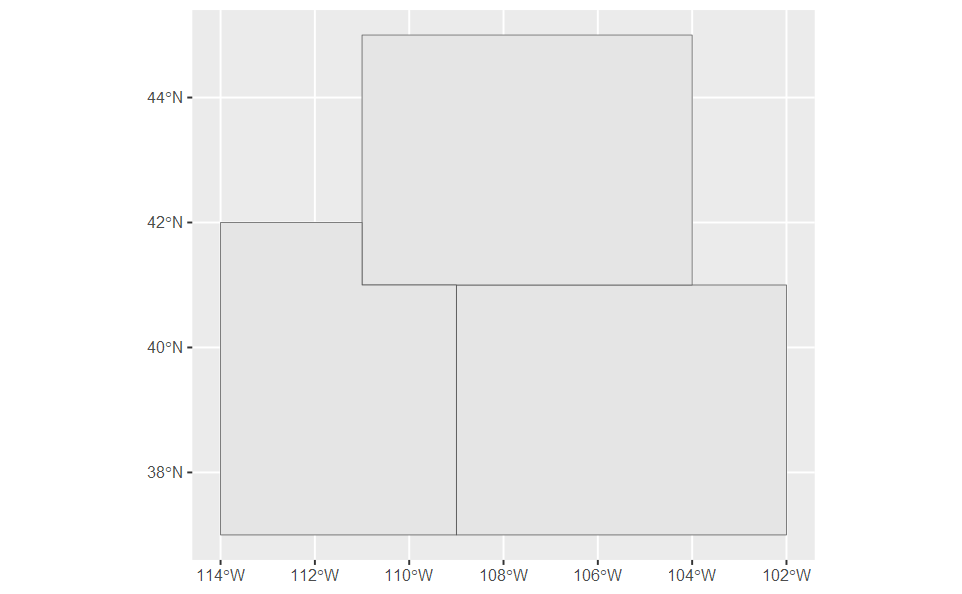
\includegraphics[width=0.75\linewidth]{img/maps.ex2} \end{center}

\begin{exercise}

Add in the code for other western states and create kind of a western US map. Go ahead and use the following code:

\begin{Shaded}
\begin{Highlighting}[]
\NormalTok{AZ }\OtherTok{\textless{}{-}} \FunctionTok{st\_polygon}\NormalTok{(}\FunctionTok{list}\NormalTok{(}\FunctionTok{rbind}\NormalTok{(}\FunctionTok{c}\NormalTok{(}\SpecialCharTok{{-}}\DecValTok{114}\NormalTok{,}\DecValTok{37}\NormalTok{),}\FunctionTok{c}\NormalTok{(}\SpecialCharTok{{-}}\DecValTok{109}\NormalTok{,}\DecValTok{37}\NormalTok{),}\FunctionTok{c}\NormalTok{(}\SpecialCharTok{{-}}\DecValTok{109}\NormalTok{,}\FloatTok{31.3}\NormalTok{),}\FunctionTok{c}\NormalTok{(}\SpecialCharTok{{-}}\DecValTok{111}\NormalTok{,}\FloatTok{31.3}\NormalTok{),}
  \FunctionTok{c}\NormalTok{(}\SpecialCharTok{{-}}\FloatTok{114.8}\NormalTok{,}\FloatTok{32.5}\NormalTok{),}\FunctionTok{c}\NormalTok{(}\SpecialCharTok{{-}}\FloatTok{114.6}\NormalTok{,}\FloatTok{32.7}\NormalTok{),}\FunctionTok{c}\NormalTok{(}\SpecialCharTok{{-}}\FloatTok{114.1}\NormalTok{,}\FloatTok{34.3}\NormalTok{),}\FunctionTok{c}\NormalTok{(}\SpecialCharTok{{-}}\FloatTok{114.5}\NormalTok{,}\DecValTok{35}\NormalTok{),}
  \FunctionTok{c}\NormalTok{(}\SpecialCharTok{{-}}\FloatTok{114.5}\NormalTok{,}\DecValTok{36}\NormalTok{),}\FunctionTok{c}\NormalTok{(}\SpecialCharTok{{-}}\DecValTok{114}\NormalTok{,}\DecValTok{36}\NormalTok{),}\FunctionTok{c}\NormalTok{(}\SpecialCharTok{{-}}\DecValTok{114}\NormalTok{,}\DecValTok{37}\NormalTok{))))}
\NormalTok{NM }\OtherTok{\textless{}{-}} \FunctionTok{st\_polygon}\NormalTok{(}\FunctionTok{list}\NormalTok{(}\FunctionTok{rbind}\NormalTok{(}\FunctionTok{c}\NormalTok{(}\SpecialCharTok{{-}}\DecValTok{109}\NormalTok{,}\DecValTok{37}\NormalTok{),}\FunctionTok{c}\NormalTok{(}\SpecialCharTok{{-}}\DecValTok{103}\NormalTok{,}\DecValTok{37}\NormalTok{),}\FunctionTok{c}\NormalTok{(}\SpecialCharTok{{-}}\DecValTok{103}\NormalTok{,}\DecValTok{32}\NormalTok{),}\FunctionTok{c}\NormalTok{(}\SpecialCharTok{{-}}\FloatTok{106.6}\NormalTok{,}\DecValTok{32}\NormalTok{),}
  \FunctionTok{c}\NormalTok{(}\SpecialCharTok{{-}}\FloatTok{106.5}\NormalTok{,}\FloatTok{31.8}\NormalTok{),}\FunctionTok{c}\NormalTok{(}\SpecialCharTok{{-}}\FloatTok{108.2}\NormalTok{,}\FloatTok{31.8}\NormalTok{),}\FunctionTok{c}\NormalTok{(}\SpecialCharTok{{-}}\FloatTok{108.2}\NormalTok{,}\FloatTok{31.3}\NormalTok{),}\FunctionTok{c}\NormalTok{(}\SpecialCharTok{{-}}\DecValTok{109}\NormalTok{,}\FloatTok{31.3}\NormalTok{),}\FunctionTok{c}\NormalTok{(}\SpecialCharTok{{-}}\DecValTok{109}\NormalTok{,}\DecValTok{37}\NormalTok{))))}
\NormalTok{CA }\OtherTok{\textless{}{-}} \FunctionTok{st\_polygon}\NormalTok{(}\FunctionTok{list}\NormalTok{(}\FunctionTok{rbind}\NormalTok{(}\FunctionTok{c}\NormalTok{(}\SpecialCharTok{{-}}\DecValTok{124}\NormalTok{,}\DecValTok{42}\NormalTok{),}\FunctionTok{c}\NormalTok{(}\SpecialCharTok{{-}}\DecValTok{120}\NormalTok{,}\DecValTok{42}\NormalTok{),}\FunctionTok{c}\NormalTok{(}\SpecialCharTok{{-}}\DecValTok{120}\NormalTok{,}\DecValTok{39}\NormalTok{),}\FunctionTok{c}\NormalTok{(}\SpecialCharTok{{-}}\FloatTok{114.5}\NormalTok{,}\DecValTok{35}\NormalTok{),}
  \FunctionTok{c}\NormalTok{(}\SpecialCharTok{{-}}\FloatTok{114.1}\NormalTok{,}\FloatTok{34.3}\NormalTok{),}\FunctionTok{c}\NormalTok{(}\SpecialCharTok{{-}}\FloatTok{114.6}\NormalTok{,}\FloatTok{32.7}\NormalTok{),}\FunctionTok{c}\NormalTok{(}\SpecialCharTok{{-}}\DecValTok{117}\NormalTok{,}\FloatTok{32.5}\NormalTok{),}\FunctionTok{c}\NormalTok{(}\SpecialCharTok{{-}}\FloatTok{118.5}\NormalTok{,}\DecValTok{34}\NormalTok{),}\FunctionTok{c}\NormalTok{(}\SpecialCharTok{{-}}\FloatTok{120.5}\NormalTok{,}\FloatTok{34.5}\NormalTok{),}
  \FunctionTok{c}\NormalTok{(}\SpecialCharTok{{-}}\DecValTok{122}\NormalTok{,}\FloatTok{36.5}\NormalTok{),}\FunctionTok{c}\NormalTok{(}\SpecialCharTok{{-}}\FloatTok{121.8}\NormalTok{,}\FloatTok{36.8}\NormalTok{),}\FunctionTok{c}\NormalTok{(}\SpecialCharTok{{-}}\DecValTok{122}\NormalTok{,}\DecValTok{37}\NormalTok{),}\FunctionTok{c}\NormalTok{(}\SpecialCharTok{{-}}\FloatTok{122.4}\NormalTok{,}\FloatTok{37.3}\NormalTok{),}\FunctionTok{c}\NormalTok{(}\SpecialCharTok{{-}}\FloatTok{122.5}\NormalTok{,}\FloatTok{37.8}\NormalTok{),}
  \FunctionTok{c}\NormalTok{(}\SpecialCharTok{{-}}\DecValTok{123}\NormalTok{,}\DecValTok{38}\NormalTok{),}\FunctionTok{c}\NormalTok{(}\SpecialCharTok{{-}}\FloatTok{123.7}\NormalTok{,}\DecValTok{39}\NormalTok{),}\FunctionTok{c}\NormalTok{(}\SpecialCharTok{{-}}\DecValTok{124}\NormalTok{,}\DecValTok{40}\NormalTok{),}\FunctionTok{c}\NormalTok{(}\SpecialCharTok{{-}}\FloatTok{124.4}\NormalTok{,}\FloatTok{40.5}\NormalTok{),}\FunctionTok{c}\NormalTok{(}\SpecialCharTok{{-}}\DecValTok{124}\NormalTok{,}\DecValTok{41}\NormalTok{),}\FunctionTok{c}\NormalTok{(}\SpecialCharTok{{-}}\DecValTok{124}\NormalTok{,}\DecValTok{42}\NormalTok{))))}
\NormalTok{NV }\OtherTok{\textless{}{-}} \FunctionTok{st\_polygon}\NormalTok{(}\FunctionTok{list}\NormalTok{(}\FunctionTok{rbind}\NormalTok{(}\FunctionTok{c}\NormalTok{(}\SpecialCharTok{{-}}\DecValTok{120}\NormalTok{,}\DecValTok{42}\NormalTok{),}\FunctionTok{c}\NormalTok{(}\SpecialCharTok{{-}}\DecValTok{114}\NormalTok{,}\DecValTok{42}\NormalTok{),}\FunctionTok{c}\NormalTok{(}\SpecialCharTok{{-}}\DecValTok{114}\NormalTok{,}\DecValTok{36}\NormalTok{),}\FunctionTok{c}\NormalTok{(}\SpecialCharTok{{-}}\FloatTok{114.5}\NormalTok{,}\DecValTok{36}\NormalTok{),}
  \FunctionTok{c}\NormalTok{(}\SpecialCharTok{{-}}\FloatTok{114.5}\NormalTok{,}\DecValTok{35}\NormalTok{),}\FunctionTok{c}\NormalTok{(}\SpecialCharTok{{-}}\DecValTok{120}\NormalTok{,}\DecValTok{39}\NormalTok{),}\FunctionTok{c}\NormalTok{(}\SpecialCharTok{{-}}\DecValTok{120}\NormalTok{,}\DecValTok{42}\NormalTok{))))}
\NormalTok{OR }\OtherTok{\textless{}{-}} \FunctionTok{st\_polygon}\NormalTok{(}\FunctionTok{list}\NormalTok{(}\FunctionTok{rbind}\NormalTok{(}\FunctionTok{c}\NormalTok{(}\SpecialCharTok{{-}}\DecValTok{124}\NormalTok{,}\DecValTok{42}\NormalTok{),}\FunctionTok{c}\NormalTok{(}\SpecialCharTok{{-}}\FloatTok{124.5}\NormalTok{,}\DecValTok{43}\NormalTok{),}
  \FunctionTok{c}\NormalTok{(}\SpecialCharTok{{-}}\DecValTok{124}\NormalTok{,}\DecValTok{46}\NormalTok{),}\FunctionTok{c}\NormalTok{(}\SpecialCharTok{{-}}\DecValTok{123}\NormalTok{,}\DecValTok{46}\NormalTok{),}\FunctionTok{c}\NormalTok{(}\SpecialCharTok{{-}}\FloatTok{122.7}\NormalTok{,}\FloatTok{45.5}\NormalTok{),}\FunctionTok{c}\NormalTok{(}\SpecialCharTok{{-}}\DecValTok{119}\NormalTok{,}\DecValTok{46}\NormalTok{),}\FunctionTok{c}\NormalTok{(}\SpecialCharTok{{-}}\DecValTok{117}\NormalTok{,}\DecValTok{46}\NormalTok{),}
  \FunctionTok{c}\NormalTok{(}\SpecialCharTok{{-}}\FloatTok{116.5}\NormalTok{,}\FloatTok{45.5}\NormalTok{),}\FunctionTok{c}\NormalTok{(}\SpecialCharTok{{-}}\FloatTok{117.2}\NormalTok{,}\FloatTok{44.5}\NormalTok{),}\FunctionTok{c}\NormalTok{(}\SpecialCharTok{{-}}\DecValTok{117}\NormalTok{,}\DecValTok{44}\NormalTok{),}
  \FunctionTok{c}\NormalTok{(}\SpecialCharTok{{-}}\DecValTok{117}\NormalTok{,}\DecValTok{42}\NormalTok{),}\FunctionTok{c}\NormalTok{(}\SpecialCharTok{{-}}\DecValTok{120}\NormalTok{,}\DecValTok{42}\NormalTok{),}\FunctionTok{c}\NormalTok{(}\SpecialCharTok{{-}}\DecValTok{124}\NormalTok{,}\DecValTok{42}\NormalTok{))))}
\NormalTok{WA }\OtherTok{\textless{}{-}} \FunctionTok{st\_polygon}\NormalTok{(}\FunctionTok{list}\NormalTok{(}\FunctionTok{rbind}\NormalTok{(}\FunctionTok{c}\NormalTok{(}\SpecialCharTok{{-}}\DecValTok{124}\NormalTok{,}\DecValTok{46}\NormalTok{),}\FunctionTok{c}\NormalTok{(}\SpecialCharTok{{-}}\FloatTok{124.8}\NormalTok{,}\FloatTok{48.4}\NormalTok{),}\FunctionTok{c}\NormalTok{(}\SpecialCharTok{{-}}\DecValTok{123}\NormalTok{,}\DecValTok{48}\NormalTok{),}
  \FunctionTok{c}\NormalTok{(}\SpecialCharTok{{-}}\DecValTok{123}\NormalTok{,}\DecValTok{49}\NormalTok{),}\FunctionTok{c}\NormalTok{(}\SpecialCharTok{{-}}\DecValTok{117}\NormalTok{,}\DecValTok{49}\NormalTok{),}
  \FunctionTok{c}\NormalTok{(}\SpecialCharTok{{-}}\DecValTok{117}\NormalTok{,}\DecValTok{46}\NormalTok{),}\FunctionTok{c}\NormalTok{(}\SpecialCharTok{{-}}\DecValTok{119}\NormalTok{,}\DecValTok{46}\NormalTok{),}\FunctionTok{c}\NormalTok{(}\SpecialCharTok{{-}}\FloatTok{122.7}\NormalTok{,}\FloatTok{45.5}\NormalTok{),}\FunctionTok{c}\NormalTok{(}\SpecialCharTok{{-}}\DecValTok{123}\NormalTok{,}\DecValTok{46}\NormalTok{),}\FunctionTok{c}\NormalTok{(}\SpecialCharTok{{-}}\DecValTok{124}\NormalTok{,}\DecValTok{46}\NormalTok{))))}
\NormalTok{ID }\OtherTok{\textless{}{-}} \FunctionTok{st\_polygon}\NormalTok{(}\FunctionTok{list}\NormalTok{(}\FunctionTok{rbind}\NormalTok{(}\FunctionTok{c}\NormalTok{(}\SpecialCharTok{{-}}\DecValTok{117}\NormalTok{,}\DecValTok{49}\NormalTok{),}
  \FunctionTok{c}\NormalTok{(}\SpecialCharTok{{-}}\DecValTok{116}\NormalTok{,}\DecValTok{49}\NormalTok{),}\FunctionTok{c}\NormalTok{(}\SpecialCharTok{{-}}\DecValTok{116}\NormalTok{,}\DecValTok{48}\NormalTok{),}\FunctionTok{c}\NormalTok{(}\SpecialCharTok{{-}}\FloatTok{114.4}\NormalTok{,}\FloatTok{46.5}\NormalTok{),}\FunctionTok{c}\NormalTok{(}\SpecialCharTok{{-}}\FloatTok{114.4}\NormalTok{,}\FloatTok{45.5}\NormalTok{),}
  \FunctionTok{c}\NormalTok{(}\SpecialCharTok{{-}}\DecValTok{114}\NormalTok{,}\FloatTok{45.6}\NormalTok{),}\FunctionTok{c}\NormalTok{(}\SpecialCharTok{{-}}\DecValTok{113}\NormalTok{,}\FloatTok{44.5}\NormalTok{),}\FunctionTok{c}\NormalTok{(}\SpecialCharTok{{-}}\DecValTok{111}\NormalTok{,}\FloatTok{44.5}\NormalTok{),}
  \FunctionTok{c}\NormalTok{(}\SpecialCharTok{{-}}\DecValTok{111}\NormalTok{,}\DecValTok{42}\NormalTok{),}\FunctionTok{c}\NormalTok{(}\SpecialCharTok{{-}}\DecValTok{114}\NormalTok{,}\DecValTok{42}\NormalTok{),}\FunctionTok{c}\NormalTok{(}\SpecialCharTok{{-}}\DecValTok{117}\NormalTok{,}\DecValTok{42}\NormalTok{),}
  \FunctionTok{c}\NormalTok{(}\SpecialCharTok{{-}}\DecValTok{117}\NormalTok{,}\DecValTok{44}\NormalTok{),}\FunctionTok{c}\NormalTok{(}\SpecialCharTok{{-}}\FloatTok{117.2}\NormalTok{,}\FloatTok{44.5}\NormalTok{),}\FunctionTok{c}\NormalTok{(}\SpecialCharTok{{-}}\FloatTok{116.5}\NormalTok{,}\FloatTok{45.5}\NormalTok{),}
  \FunctionTok{c}\NormalTok{(}\SpecialCharTok{{-}}\DecValTok{117}\NormalTok{,}\DecValTok{46}\NormalTok{),}\FunctionTok{c}\NormalTok{(}\SpecialCharTok{{-}}\DecValTok{117}\NormalTok{,}\DecValTok{49}\NormalTok{))))}
\NormalTok{MT }\OtherTok{\textless{}{-}} \FunctionTok{st\_polygon}\NormalTok{(}\FunctionTok{list}\NormalTok{(}\FunctionTok{rbind}\NormalTok{(}\FunctionTok{c}\NormalTok{(}\SpecialCharTok{{-}}\DecValTok{116}\NormalTok{,}\DecValTok{49}\NormalTok{),}\FunctionTok{c}\NormalTok{(}\SpecialCharTok{{-}}\DecValTok{104}\NormalTok{,}\DecValTok{49}\NormalTok{),}
  \FunctionTok{c}\NormalTok{(}\SpecialCharTok{{-}}\DecValTok{104}\NormalTok{,}\DecValTok{45}\NormalTok{),}\FunctionTok{c}\NormalTok{(}\SpecialCharTok{{-}}\DecValTok{111}\NormalTok{,}\DecValTok{45}\NormalTok{),}
  \FunctionTok{c}\NormalTok{(}\SpecialCharTok{{-}}\DecValTok{111}\NormalTok{,}\FloatTok{44.5}\NormalTok{),}\FunctionTok{c}\NormalTok{(}\SpecialCharTok{{-}}\DecValTok{113}\NormalTok{,}\FloatTok{44.5}\NormalTok{),}\FunctionTok{c}\NormalTok{(}\SpecialCharTok{{-}}\DecValTok{114}\NormalTok{,}\FloatTok{45.6}\NormalTok{),}\FunctionTok{c}\NormalTok{(}\SpecialCharTok{{-}}\FloatTok{114.4}\NormalTok{,}\FloatTok{45.5}\NormalTok{),}
  \FunctionTok{c}\NormalTok{(}\SpecialCharTok{{-}}\FloatTok{114.4}\NormalTok{,}\FloatTok{46.5}\NormalTok{),}\FunctionTok{c}\NormalTok{(}\SpecialCharTok{{-}}\DecValTok{116}\NormalTok{,}\DecValTok{48}\NormalTok{),}\FunctionTok{c}\NormalTok{(}\SpecialCharTok{{-}}\DecValTok{116}\NormalTok{,}\DecValTok{49}\NormalTok{))))}
\end{Highlighting}
\end{Shaded}

Then build sfcWestStates from these geometries using the methods in 6.1.1.2, specifying GCS (4326) as the crs, and plot with methods from 6.6.

\begin{center}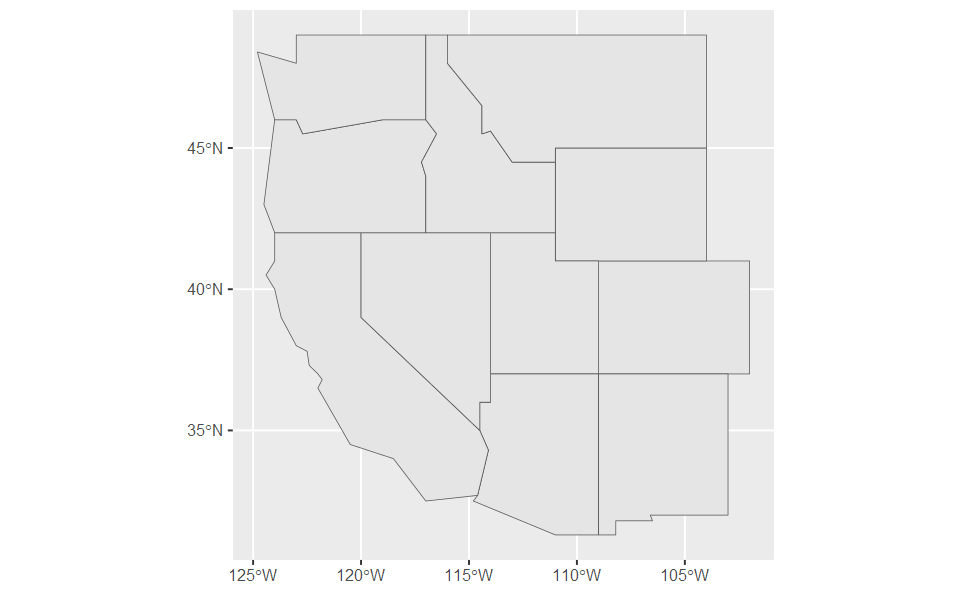
\includegraphics[width=0.75\linewidth]{img/maps.ex3} \end{center}

\end{exercise}

\begin{exercise}

Create western states using methods from 6.1.1.3, adding the fields \texttt{name}, \texttt{abb}, \texttt{area\_sqkm}, and \texttt{population}, and create a map labeling with the name. Note that the added fields need to be in the same order as the boundaries created above. Also remember to make the area and pop variables numeric, which will happen if they're brought in as a vector along with character variables. Apply methods from 6.6 and references on R color systems to get higher values shaded darker, to follow cartographic figure-ground contrast convention.

\begin{itemize}
\tightlist
\item
  Colorado, CO, 269837, 5758736
\item
  Wyoming, WY, 253600, 578759
\item
  Utah, UT, 84899, 3205958
\item
  Arizona, AZ, 295234, 7278717
\item
  New Mexico, NM, 314917, 2096829
\item
  California, CA, 423970, 39368078
\item
  Nevada, NV, 286382, 3080156
\item
  Oregon, OR, 254806, 4237256
\item
  Washington, WA, 184827, 7705281
\item
  Idaho, ID, 216443, 1839106
\item
  Montana, MT, 380800, 1085407
\end{itemize}

\end{exercise}

\begin{center}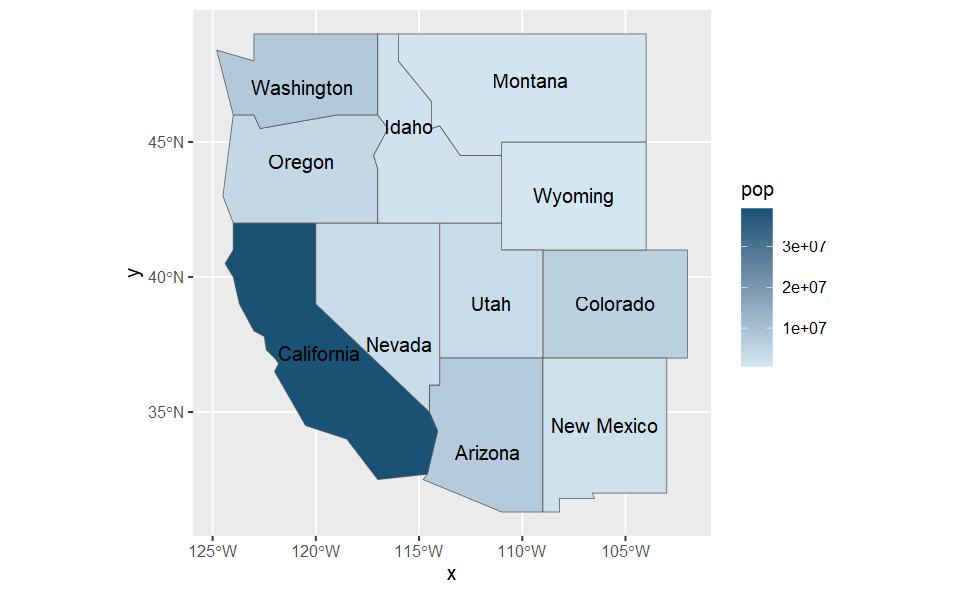
\includegraphics[width=0.75\linewidth]{img/maps.ex4} \end{center}

\begin{exercise}
Store the W\_States as a shape file in the data folder with st\_write. (Look up how to use st\_write with ?st\_write -- it's pretty simple.) Note that this will fail if it already exists, so include the parameter \texttt{delete\_layer\ =\ TRUE} to allow overwrite.
\end{exercise}

\begin{exercise}
\textbf{Highest Peaks}: Create a tibble for the highest peaks in the western states, with the following names, elevations in m, longitude and latitude, use methods from 6.1.2 to create spatial data from it, and add them to that map. Then write the shapefile out again as ``data/peaks.shp'' again allowing overwriting.

\begin{itemize}
\tightlist
\item
  Wheeler Peak, 4011, -105.4, 36.5
\item
  Mt. Whitney, 4421, -118.2, 36.5
\item
  Boundary Peak, 4007, -118.35, 37.9
\item
  Kings Peak, 4120, -110.3, 40.8
\item
  Gannett Peak, 4209, -109, 43.2
\item
  Mt. Elbert, 4401, -106.4, 39.1
\item
  Humphreys Peak, 3852, -111.7, 35.4
\item
  Mt. Hood, 3428, -121.7, 45.4
\item
  Mt. Rainier, 4392, -121.8, 46.9
\item
  Borah Peak, 3859, -113.8, 44.1
\item
  Granite Peak, 3903, -109.8, 45.1
\end{itemize}

Note: the easiest way to do this is with the method in 3.2.2, using the above data.
\end{exercise}

And finally create a map showing peaks labeled and the states filled based on area. Use cartographic methods from either 6.6 or 6.8.

\begin{center}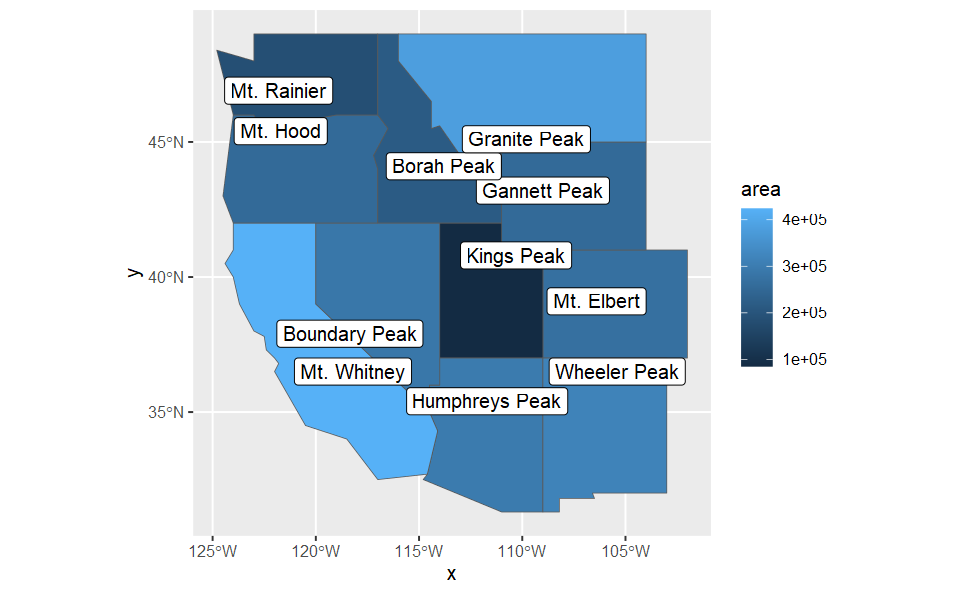
\includegraphics[width=0.5\linewidth]{img/maps.ex6} \end{center}

\begin{exercise}
\textbf{California freeways}. From the CA\_counties and CAfreeways feature data in igisci, make a simple map (using methods from 6.6), with freeways colored red.
\end{exercise}

\begin{center}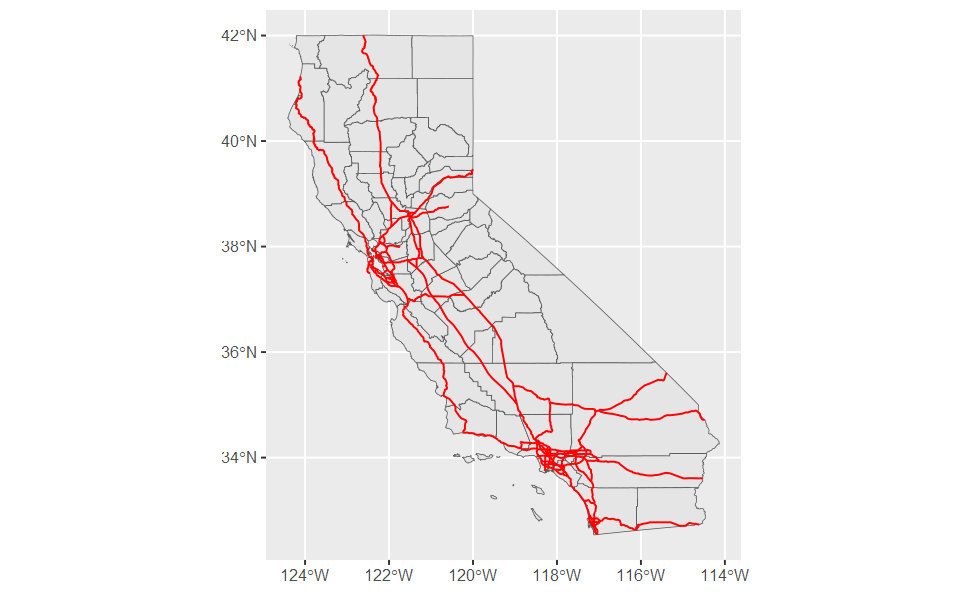
\includegraphics[width=0.75\linewidth]{img/maps.ex7} \end{center}

\begin{exercise}
After adding the terra library, create a raster from the built-in \texttt{volcano} matrix of elevations from Auckland's \textbf{Maunga Whau Volcano}, and use plot() to display it. We'd do more with that dataset, but we don't know what the cell size is.
\end{exercise}

\begin{center}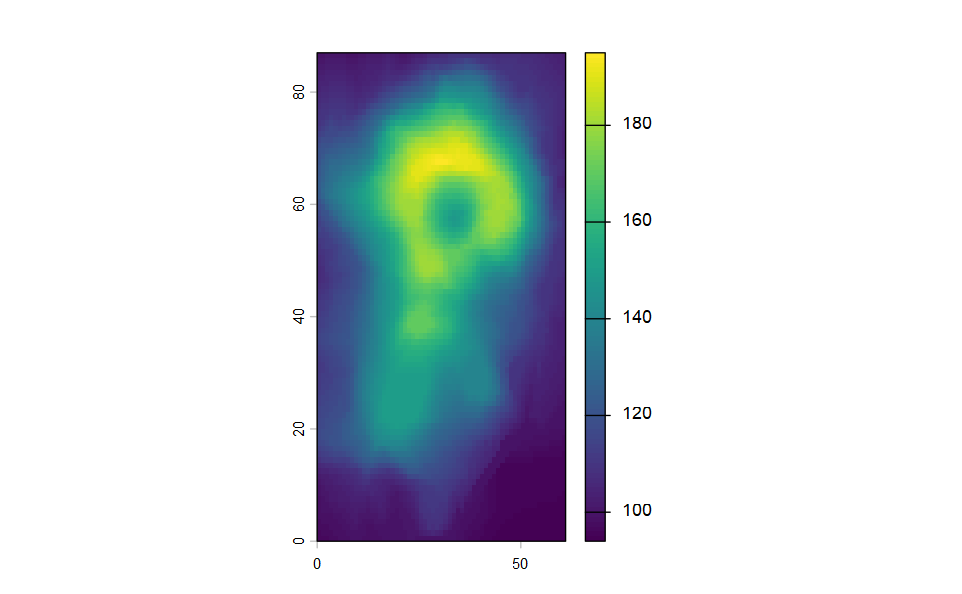
\includegraphics[width=0.75\linewidth]{img/maps.ex8} \end{center}

\begin{exercise}
\textbf{Western States tmap}: Use tmap to create a map from the W\_States (polygons) and peaksp (points) data we created earlier. Include a basemap with no labels (I've used ``CartoDB.VoyagerNoLabels'' and Esri.WorldShadedRelief''). Hints: you'll want to use tm\_text with text set to ``peak'' to label the points. Use this as an opportunity to test the geospatial data you've written earlier by using methods from 6.1.4 to read them. Experiment with \texttt{tm\_symbol} sizes, \texttt{xmod}, and \texttt{ymod} settings with \texttt{tm\_text}. A tm\_text option we haven't used before is to left-justify text by including \texttt{options=opt\_tm\_text(just="left")}
\end{exercise}

\begin{center}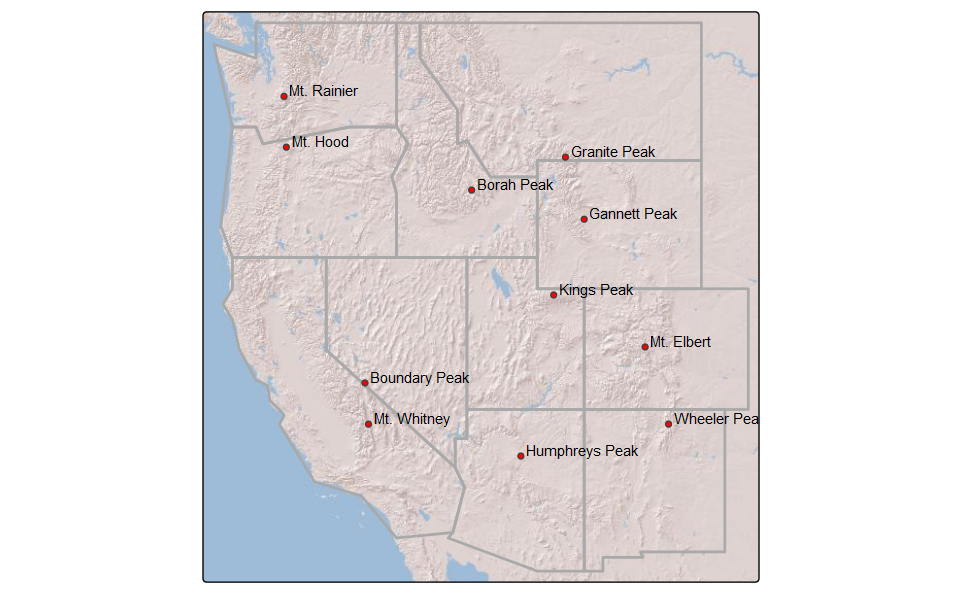
\includegraphics[width=0.75\linewidth]{img/maps.ex9} \end{center}

\begin{exercise}
\textbf{tmap view mode}. Also using the western states data, create a similar tmap in view mode, but setting the basemap server to \texttt{"Esri.WorldImagery"}.
\end{exercise}

\begin{center}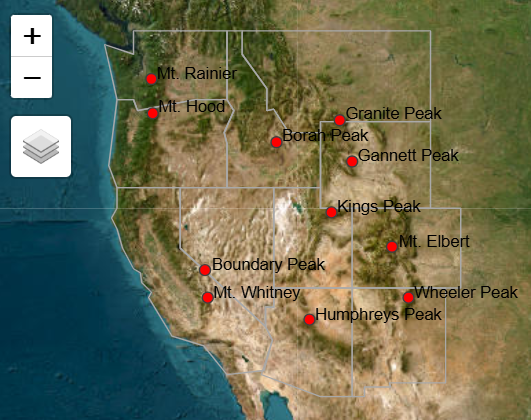
\includegraphics[width=0.75\linewidth]{img/tmapExample} \end{center}

\chapter{Spatial Analysis}\label{spatial-analysis}

\begin{center}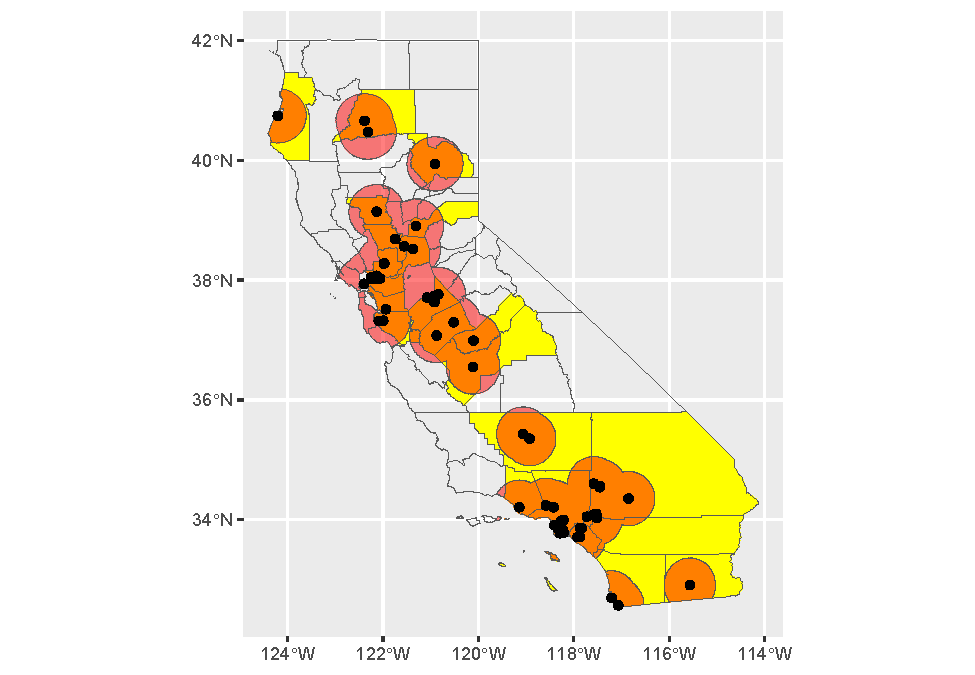
\includegraphics[width=0.75\linewidth]{EnvDataScience_files/figure-latex/unnamed-chunk-198-1} \end{center}

\index{spatial analysis}Spatial analysis provides an expansive analytical landscape with theoretical underpinnings dating to at least the 1950s (Berry and Marble (\citeproc{ref-SpatialAnalysis}{1968})), contributing to the development of geographic information systems as well as spatial tools in more statistically oriented programming environments like R. We won't attempt to approach any thorough coverage of these methods, and we would refer the reader for more focused consideration using R-based methods to sources such as Lovelace et al. (\citeproc{ref-Geocomputation}{2019}) and Hijmans (\citeproc{ref-rspatial}{n.d.}).

In this chapter, we'll continue working with spatial data, and explore spatial analysis methods. We'll look at a selection of useful geospatial abstraction and analysis methods, what are also called \index{geoprocessing}\emph{geoprocessing} tools in a GIS. The R Spatial world has grown in recent years to include an increasingly good array of tools. This chapter will focus on \emph{vector} GIS methods, and here we don't mean the same thing as the vector data objects in R nomenclature (Python's pandas package, which uses a similar data structure, calls these ``series'' instead of vectors), but instead on feature geometries and their spatial relationships based on the coordinate referencing system.

\section{Data Frame Operations}\label{data-frame-operations}

\index{data frame operations for spatial analysis}But before we get into those specifically spatial operations, it's important to remember that feature data at least are also data frames, so we can use the methods we already know with them. For instance, we can look at properties of variables and then filter for features that meet a criterion, like all climate station points at greater than 2,000 m elevation, or all above 38°N latitude. To be able to work with latitude as a variable, we'll need to use \texttt{remove=F} (the default is to remove them) to retain them when we use \texttt{st\_as\_sf}.

\textbf{Adding a basemap with maptiles}: \index{basemap}We'd like to have a basemap, so we'll create one with the \index{maptiles}\texttt{maptiles} package (install if you don't have it.) \emph{Warning: the \texttt{get\_tiles} function goes online to get the basemap data, so if you don't have a good internet connection or the site goes down, this may fail.} We can then display the basemap with \texttt{tm\_rgb}.

For temperature, we'll use a continuous color scale of ``hcl.blue\_red'' to go from cold (blue) to warm (red).

\begin{Shaded}
\begin{Highlighting}[]
\FunctionTok{library}\NormalTok{(tmap); }\FunctionTok{library}\NormalTok{(RColorBrewer); }\FunctionTok{library}\NormalTok{(sf); }\FunctionTok{library}\NormalTok{(tidyverse); }
\FunctionTok{library}\NormalTok{(maptiles); }\FunctionTok{library}\NormalTok{(igisci)}
\FunctionTok{tmap\_mode}\NormalTok{(}\StringTok{"plot"}\NormalTok{)}
\NormalTok{newname }\OtherTok{\textless{}{-}} \FunctionTok{unique}\NormalTok{(}\FunctionTok{str\_sub}\NormalTok{(sierraFeb}\SpecialCharTok{$}\NormalTok{STATION\_NAME, }\DecValTok{1}\NormalTok{, }
                          \FunctionTok{str\_locate}\NormalTok{(sierraFeb}\SpecialCharTok{$}\NormalTok{STATION\_NAME, }\StringTok{","}\NormalTok{)}\SpecialCharTok{{-}}\DecValTok{1}\NormalTok{))}
\NormalTok{sierraFeb2000 }\OtherTok{\textless{}{-}} \FunctionTok{st\_as\_sf}\NormalTok{(}\FunctionTok{bind\_cols}\NormalTok{(sierraFeb,}\AttributeTok{STATION=}\NormalTok{newname) }\SpecialCharTok{\%\textgreater{}\%} 
\NormalTok{                          dplyr}\SpecialCharTok{::}\FunctionTok{select}\NormalTok{(}\SpecialCharTok{{-}}\NormalTok{STATION\_NAME) }\SpecialCharTok{\%\textgreater{}\%} 
                          \FunctionTok{filter}\NormalTok{(ELEVATION }\SpecialCharTok{\textgreater{}=} \DecValTok{2000}\NormalTok{, }\SpecialCharTok{!}\FunctionTok{is.na}\NormalTok{(TEMPERATURE)), }
                 \AttributeTok{coords=}\FunctionTok{c}\NormalTok{(}\StringTok{"LONGITUDE"}\NormalTok{,}\StringTok{"LATITUDE"}\NormalTok{), }\AttributeTok{remove=}\NormalTok{F, }\AttributeTok{crs=}\DecValTok{4326}\NormalTok{)}
\NormalTok{bounds}\OtherTok{=}\NormalTok{tmaptools}\SpecialCharTok{::}\FunctionTok{bb}\NormalTok{(sierraFeb2000, }\AttributeTok{ext=}\FloatTok{1.2}\NormalTok{)}
\NormalTok{sierraBase }\OtherTok{\textless{}{-}} \FunctionTok{get\_tiles}\NormalTok{(sierraFeb2000, }\AttributeTok{provider=}\StringTok{"OpenStreetMap"}\NormalTok{)}
\FunctionTok{tm\_shape}\NormalTok{(sierraBase, }\AttributeTok{bbox=}\NormalTok{bounds) }\SpecialCharTok{+} 
  \FunctionTok{tm\_rgb}\NormalTok{() }\SpecialCharTok{+} \CommentTok{\# tm\_mv("red", "green", "blue"), col.scale = tm\_scale\_rgb(maxValue = 255)) +}
  \FunctionTok{tm\_shape}\NormalTok{(sierraFeb2000) }\SpecialCharTok{+} 
  \FunctionTok{tm\_dots}\NormalTok{(}\AttributeTok{fill =}  \StringTok{"TEMPERATURE"}\NormalTok{, }\CommentTok{\#midpoint=NA,}
          \AttributeTok{fill.scale=}\FunctionTok{tm\_scale\_continuous}\NormalTok{(}\AttributeTok{values=}\StringTok{"hcl.blue\_red"}\NormalTok{),}
          \AttributeTok{size=}\DecValTok{1}\NormalTok{, }\AttributeTok{fill.legend=}\FunctionTok{tm\_legend}\NormalTok{(}\AttributeTok{frame=}\NormalTok{F)) }\SpecialCharTok{+}
  \FunctionTok{tm\_text}\NormalTok{(}\AttributeTok{text =} \StringTok{"STATION"}\NormalTok{, }\AttributeTok{size=}\FloatTok{0.5}\NormalTok{, }\AttributeTok{auto.placement=}\NormalTok{T, }\AttributeTok{xmod=}\FloatTok{0.5}\NormalTok{, }\AttributeTok{ymod=}\FloatTok{0.5}\NormalTok{) }\SpecialCharTok{+}
  \FunctionTok{tm\_graticules}\NormalTok{(}\AttributeTok{lines=}\NormalTok{F)}
\end{Highlighting}
\end{Shaded}

\begin{center}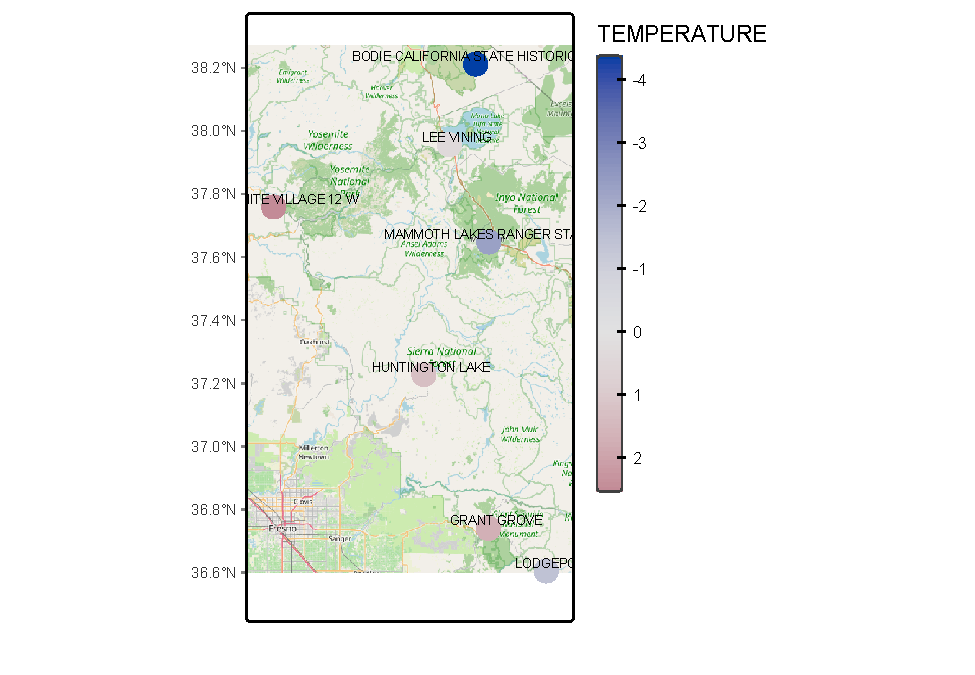
\includegraphics[width=0.75\linewidth]{EnvDataScience_files/figure-latex/unnamed-chunk-199-1} \end{center}

\begin{quote}
Note that you could also use \texttt{tm\_basemap} for this, but for some reason in this case the \texttt{maptiles::get\_tiles} approach works better.
\end{quote}

\begin{Shaded}
\begin{Highlighting}[]
\NormalTok{basemap }\OtherTok{\textless{}{-}} \FunctionTok{get\_tiles}\NormalTok{(CA\_counties, }\AttributeTok{provider=}\StringTok{"Esri.WorldTerrain"}\NormalTok{)}
\NormalTok{cols }\OtherTok{=} \FunctionTok{names}\NormalTok{(basemap)}
\NormalTok{bounds}\OtherTok{=}\NormalTok{tmaptools}\SpecialCharTok{::}\FunctionTok{bb}\NormalTok{(sierraFeb2000, }\AttributeTok{ext=}\FloatTok{1.2}\NormalTok{)}
\NormalTok{CA }\OtherTok{\textless{}{-}} \FunctionTok{tm\_shape}\NormalTok{(basemap,}\AttributeTok{bbox=}\NormalTok{bounds) }\SpecialCharTok{+} \FunctionTok{tm\_rgb}\NormalTok{() }\SpecialCharTok{+} \CommentTok{\#tm\_mv(cols[1],cols[2],cols[3])) +}
      \FunctionTok{tm\_shape}\NormalTok{(CA\_counties) }\SpecialCharTok{+} \FunctionTok{tm\_borders}\NormalTok{(}\AttributeTok{lwd=}\DecValTok{1}\NormalTok{, }\AttributeTok{col=}\StringTok{"red"}\NormalTok{) }\SpecialCharTok{+}
      \FunctionTok{tm\_graticules}\NormalTok{(}\AttributeTok{lines=}\NormalTok{F,}\AttributeTok{labels.rot=}\FunctionTok{c}\NormalTok{(}\DecValTok{0}\NormalTok{,}\DecValTok{90}\NormalTok{)) }\SpecialCharTok{+}
      \FunctionTok{tm\_title}\NormalTok{(}\StringTok{"CA counties on basemap"}\NormalTok{)}
\end{Highlighting}
\end{Shaded}

Now let's include LATITUDE. Let's see what we get by filtering for both \texttt{ELEVATION\ \textgreater{}=\ 2000} and \texttt{LATITUDE\ \textgreater{}=\ 38}:

\begin{Shaded}
\begin{Highlighting}[]
\NormalTok{sierraFeb2000 }\SpecialCharTok{\%\textgreater{}\%}
  \FunctionTok{filter}\NormalTok{(ELEVATION }\SpecialCharTok{\textgreater{}=} \DecValTok{2000} \SpecialCharTok{\&}\NormalTok{ LATITUDE }\SpecialCharTok{\textgreater{}=} \DecValTok{38}\NormalTok{)}
\end{Highlighting}
\end{Shaded}

\begin{verbatim}
## Simple feature collection with 1 feature and 7 fields
## Geometry type: POINT
## Dimension:     XY
## Bounding box:  xmin: -119.0142 ymin: 38.2119 xmax: -119.0142 ymax: 38.2119
## Geodetic CRS:  WGS 84
## # A tibble: 1 x 8
##   COUNTY ELEVATION LATITUDE LONGITUDE PRECIPITATION TEMPERATURE STATION         
## * <fct>      <dbl>    <dbl>     <dbl>         <dbl>       <dbl> <chr>           
## 1 Mono       2551.     38.2     -119.          39.6        -4.4 BODIE CALIFORNI~
## # i 1 more variable: geometry <POINT [°]>
\end{verbatim}

The only one left is Bodie (Figure \ref{fig:spanlBodie}). Maybe that's why Bodie, a ghost town now, has such a reputation for being so friggin' cold (at least for California). I've been snowed on there in summer.

\begin{figure}

{\centering 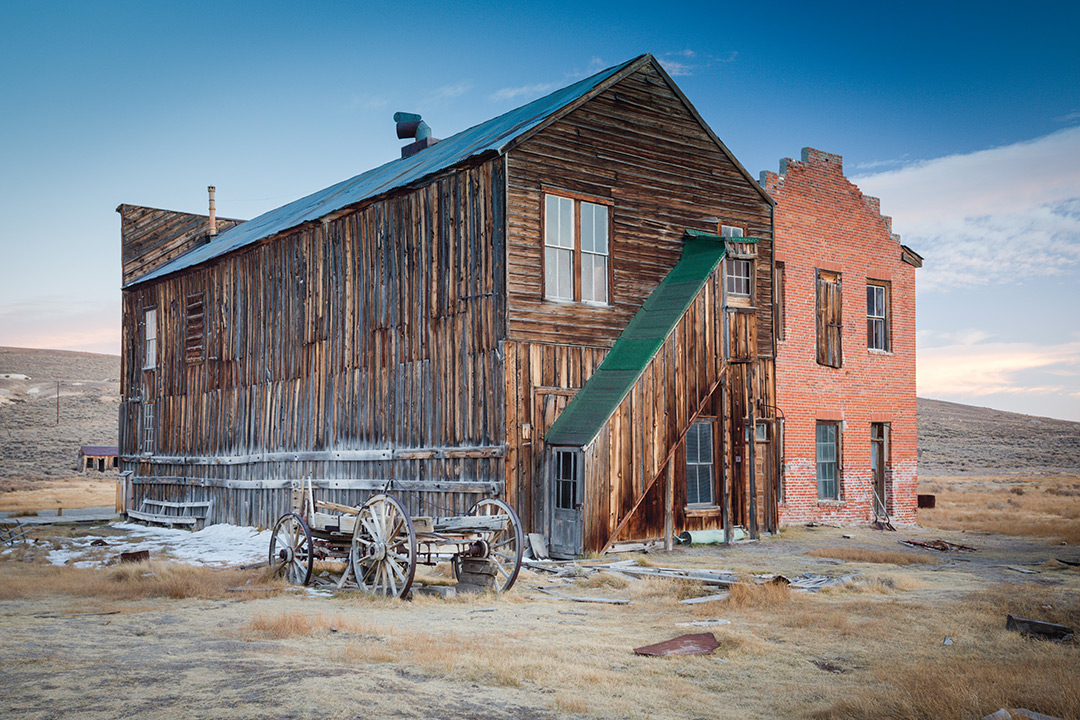
\includegraphics[width=0.75\linewidth]{img/BodieSHP_Gallery_11} 

}

\caption{A Bodie scene, from Bodie State Historic Park (https://www.parks.ca.gov/)}\label{fig:spanlBodie}
\end{figure}

\subsection{Using grouped summaries, and filtering by a selection}\label{GroupedSummaries}

\index{grouped summaries}We've been using February Sierra climate data for demonstrating various things, but this wasn't the original form of the data downloaded, so let's look at the original data and use some dplyr methods to restructure it, in this case to derive annual summaries. We'll use the monthly normals to derive annual values.

We looked at the very useful \texttt{group\_by\ ...\ summarize()} group-summary process earlier \ref{group-summary}. We'll use this and a selection process to create an annual Sierra climate dataframe we can map and analyze. The California monthly normals were downloaded from the National Centers for Environmental Information at NOAA, where you can select desired parameters, monthly normals as frequency, and limit to one state.

\begin{itemize}
\tightlist
\item
  \url{https://www.ncei.noaa.gov/}
\item
  \url{https://www.ncei.noaa.gov/products/land-based-station/us-climate-normals}
\item
  \url{https://www.ncei.noaa.gov/access/search/data-search/normals-monthly-1991-2020}
\end{itemize}

First we'll have a quick look at the data to see how it's structured. These were downloaded as monthly normals for the State of California, as of 2010, so there are 12 months coded \texttt{201001}:\texttt{201012}, with obviously the same \texttt{ELEVATION}, \texttt{LATITUDE}, and \texttt{LONGITUDE}, but monthly values for climate data like \texttt{MLY-PRCP-NORMAL}, etc.

\begin{Shaded}
\begin{Highlighting}[]
\FunctionTok{head}\NormalTok{(}\FunctionTok{read\_csv}\NormalTok{(}\FunctionTok{ex}\NormalTok{(}\StringTok{"sierra/908277.csv"}\NormalTok{)),}\AttributeTok{n=}\DecValTok{15}\NormalTok{)}
\end{Highlighting}
\end{Shaded}

\begin{verbatim}
## # A tibble: 15 x 11
##    STATION    STATION_NAME ELEVATION LATITUDE LONGITUDE   DATE `MLY-PRCP-NORMAL`
##    <chr>      <chr>        <chr>     <chr>    <chr>      <dbl>             <dbl>
##  1 GHCND:USC~ TWENTYNINE ~ 602       34.12806 -116.036~ 201001             13.2 
##  2 GHCND:USC~ TWENTYNINE ~ 602       34.12806 -116.036~ 201002             15.0 
##  3 GHCND:USC~ TWENTYNINE ~ 602       34.12806 -116.036~ 201003             11.4 
##  4 GHCND:USC~ TWENTYNINE ~ 602       34.12806 -116.036~ 201004              3.3 
##  5 GHCND:USC~ TWENTYNINE ~ 602       34.12806 -116.036~ 201005              2.29
##  6 GHCND:USC~ TWENTYNINE ~ 602       34.12806 -116.036~ 201006              0.25
##  7 GHCND:USC~ TWENTYNINE ~ 602       34.12806 -116.036~ 201007             12.2 
##  8 GHCND:USC~ TWENTYNINE ~ 602       34.12806 -116.036~ 201008             20.6 
##  9 GHCND:USC~ TWENTYNINE ~ 602       34.12806 -116.036~ 201009             10.2 
## 10 GHCND:USC~ TWENTYNINE ~ 602       34.12806 -116.036~ 201010              5.08
## 11 GHCND:USC~ TWENTYNINE ~ 602       34.12806 -116.036~ 201011              5.08
## 12 GHCND:USC~ TWENTYNINE ~ 602       34.12806 -116.036~ 201012             14.7 
## 13 GHCND:USC~ BUTTONWILLO~ 82        35.4047  -119.4731 201001             32.5 
## 14 GHCND:USC~ BUTTONWILLO~ 82        35.4047  -119.4731 201002             30.0 
## 15 GHCND:USC~ BUTTONWILLO~ 82        35.4047  -119.4731 201003             30.7 
## # i 4 more variables: `MLY-SNOW-NORMAL` <dbl>, `MLY-TAVG-NORMAL` <dbl>,
## #   `MLY-TMAX-NORMAL` <dbl>, `MLY-TMIN-NORMAL` <dbl>
\end{verbatim}

To get just the Sierra data, it seemed easiest to just provide a list of relevant county names to \index{filter}filter the counties, do a bit of field renaming, then read in a previously created selection of Sierra weather/climate stations.

\begin{Shaded}
\begin{Highlighting}[]
\NormalTok{sierraCounties }\OtherTok{\textless{}{-}} \FunctionTok{st\_make\_valid}\NormalTok{(CA\_counties) }\SpecialCharTok{\%\textgreater{}\%}
  \FunctionTok{filter}\NormalTok{(NAME }\SpecialCharTok{\%in\%} \FunctionTok{c}\NormalTok{(}\StringTok{"Alpine"}\NormalTok{,}\StringTok{"Amador"}\NormalTok{,}\StringTok{"Butte"}\NormalTok{,}\StringTok{"Calaveras"}\NormalTok{,}\StringTok{"El Dorado"}\NormalTok{,}
                     \StringTok{"Fresno"}\NormalTok{,}\StringTok{"Inyo"}\NormalTok{,}\StringTok{"Kern"}\NormalTok{,}\StringTok{"Lassen"}\NormalTok{,}\StringTok{"Madera"}\NormalTok{,}\StringTok{"Mariposa"}\NormalTok{,}
                     \StringTok{"Mono"}\NormalTok{,}\StringTok{"Nevada"}\NormalTok{,}\StringTok{"Placer"}\NormalTok{,}\StringTok{"Plumas"}\NormalTok{,}\StringTok{"Sacramento"}\NormalTok{,}\StringTok{"Shasta"}\NormalTok{,}
                     \StringTok{"Sierra"}\NormalTok{,}\StringTok{"Tehama"}\NormalTok{,}\StringTok{"Tulare"}\NormalTok{,}\StringTok{"Tuolumne"}\NormalTok{,}\StringTok{"Yuba"}\NormalTok{))}
\NormalTok{normals }\OtherTok{\textless{}{-}} \FunctionTok{read\_csv}\NormalTok{(}\FunctionTok{ex}\NormalTok{(}\StringTok{"sierra/908277.csv"}\NormalTok{)) }\SpecialCharTok{\%\textgreater{}\%}
  \FunctionTok{mutate}\NormalTok{(}\AttributeTok{STATION =} \FunctionTok{str\_sub}\NormalTok{(STATION,}\DecValTok{7}\NormalTok{,}\FunctionTok{str\_length}\NormalTok{(STATION)))}
\NormalTok{sierraStations }\OtherTok{\textless{}{-}} \FunctionTok{read\_csv}\NormalTok{(}\FunctionTok{ex}\NormalTok{(}\StringTok{"sierra/sierraStations.csv"}\NormalTok{))}
\end{Highlighting}
\end{Shaded}

To get annual values, we'll want to use the stations as groups in a \index{group\_by}\texttt{group\_by} \texttt{\%\textgreater{}\%} \texttt{summarize} process. For values that stay the same for a station (\texttt{LONGITUDE}, \texttt{LATITUDE}, \texttt{ELEVATION}), we'll use \texttt{first()} to get just one of the 12 identical monthly values. For values that vary monthly, we'll \texttt{sum()} the monthly precipitations and get the \texttt{mean()} of monthly temperatures to get appropriate annual values. We'll also use a \texttt{right\_join} to keep only the stations that are in the Sierra. \emph{Have a look at this script to make sure you understand what it's doing; it's got several elements you've been introduced to before, and that you should understand.} At the end, we'll use \texttt{st\_as\_sf} to make sf data out of the data frame, and retain the \texttt{LONGITUDE} and \texttt{LATITUDE} variables in case we want to use them as separate variables (Figure \ref{fig:spanlSierraData}).

\begin{Shaded}
\begin{Highlighting}[]
\NormalTok{sierraAnnual }\OtherTok{\textless{}{-}} \FunctionTok{right\_join}\NormalTok{(sierraStations,normals,}\AttributeTok{by=}\StringTok{"STATION"}\NormalTok{) }\SpecialCharTok{\%\textgreater{}\%}
  \FunctionTok{filter}\NormalTok{(}\SpecialCharTok{!}\FunctionTok{is.na}\NormalTok{(STATION\_NA)) }\SpecialCharTok{\%\textgreater{}\%} 
\NormalTok{    dplyr}\SpecialCharTok{::}\FunctionTok{select}\NormalTok{(}\SpecialCharTok{{-}}\NormalTok{STATION\_NA) }\SpecialCharTok{\%\textgreater{}\%}
    \FunctionTok{group\_by}\NormalTok{(STATION\_NAME) }\SpecialCharTok{\%\textgreater{}\%} \FunctionTok{summarize}\NormalTok{(}\AttributeTok{LONGITUDE =} \FunctionTok{first}\NormalTok{(LONGITUDE),}
                                         \AttributeTok{LATITUDE =} \FunctionTok{first}\NormalTok{(LATITUDE),}
                                         \AttributeTok{ELEVATION =} \FunctionTok{first}\NormalTok{(ELEVATION),}
                                         \AttributeTok{PRECIPITATION =} \FunctionTok{sum}\NormalTok{(}\StringTok{\textasciigrave{}}\AttributeTok{MLY{-}PRCP{-}NORMAL}\StringTok{\textasciigrave{}}\NormalTok{),}
                                         \AttributeTok{TEMPERATURE =} \FunctionTok{mean}\NormalTok{(}\StringTok{\textasciigrave{}}\AttributeTok{MLY{-}TAVG{-}NORMAL}\StringTok{\textasciigrave{}}\NormalTok{)) }\SpecialCharTok{\%\textgreater{}\%}
    \FunctionTok{mutate}\NormalTok{(}\AttributeTok{STATION\_NAME =} \FunctionTok{str\_sub}\NormalTok{(STATION\_NAME,}\DecValTok{1}\NormalTok{,}\FunctionTok{str\_length}\NormalTok{(STATION\_NAME)}\SpecialCharTok{{-}}\DecValTok{6}\NormalTok{)) }\SpecialCharTok{\%\textgreater{}\%}
  \FunctionTok{filter}\NormalTok{(PRECIPITATION }\SpecialCharTok{\textgreater{}} \DecValTok{0}\NormalTok{) }\SpecialCharTok{\%\textgreater{}\%} \FunctionTok{filter}\NormalTok{(TEMPERATURE }\SpecialCharTok{\textgreater{}} \SpecialCharTok{{-}}\DecValTok{100}\NormalTok{) }\SpecialCharTok{\%\textgreater{}\%}
  \FunctionTok{st\_as\_sf}\NormalTok{(}\AttributeTok{coords =} \FunctionTok{c}\NormalTok{(}\StringTok{"LONGITUDE"}\NormalTok{, }\StringTok{"LATITUDE"}\NormalTok{), }\AttributeTok{crs=}\DecValTok{4326}\NormalTok{, }\AttributeTok{remove=}\NormalTok{F)}
\FunctionTok{ggplot}\NormalTok{() }\SpecialCharTok{+} 
  \FunctionTok{geom\_sf}\NormalTok{(}\AttributeTok{data=}\NormalTok{CA\_counties, }\FunctionTok{aes}\NormalTok{(), }\AttributeTok{fill=}\StringTok{"gray"}\NormalTok{) }\SpecialCharTok{+}
  \FunctionTok{geom\_sf}\NormalTok{(}\AttributeTok{data=}\NormalTok{sierraCounties, }\FunctionTok{aes}\NormalTok{(), }\AttributeTok{fill=}\StringTok{"white"}\NormalTok{) }\SpecialCharTok{+} 
  \FunctionTok{geom\_sf}\NormalTok{(}\AttributeTok{data=}\NormalTok{sierraAnnual, }\FunctionTok{aes}\NormalTok{(}\AttributeTok{col=}\NormalTok{PRECIPITATION)) }\SpecialCharTok{+}
  \FunctionTok{scale\_color\_gradient}\NormalTok{(}\AttributeTok{low=}\StringTok{"orange"}\NormalTok{, }\AttributeTok{high=}\StringTok{"blue"}\NormalTok{) }
\end{Highlighting}
\end{Shaded}

\begin{figure}

{\centering 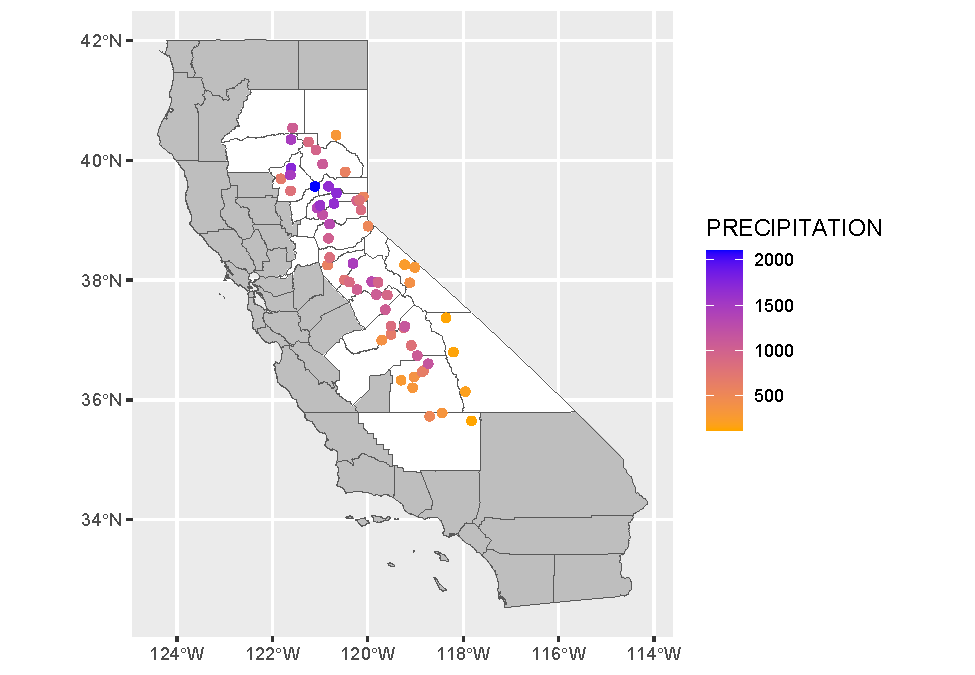
\includegraphics[width=0.75\linewidth]{EnvDataScience_files/figure-latex/spanlSierraData-1} 

}

\caption{Sierra data}\label{fig:spanlSierraData}
\end{figure}

\section{Spatial Analysis Operations}\label{spatial-analysis-operations}

Again, there is a lot more to spatial analysis than we have time to cover. But we'll explore some particularly useful spatial analysis operations, especially those that contribute to statistical analysis methods we'll be looking at soon. We'll start by continuing to look at subsetting or filtering methods, but ones that use spatial relationships to identify what we want to retain or remove from consideration.

\subsection{Using topology to subset}\label{using-topology-to-subset}

\index{topological subset}Using spatial relationships can be useful in filtering our data, and there are quite a few topological relationships that can be explored. See Lovelace et al. (\citeproc{ref-Geocomputation}{2019}) for a lot more about topological operations. We'll look at a relatively simple one that identifies whether a feature is within another one, and apply this method to filter for features within a selection of five counties, which we'll start by identifying by name.

\begin{Shaded}
\begin{Highlighting}[]
\NormalTok{nSierraCo }\OtherTok{\textless{}{-}}\NormalTok{ CA\_counties }\SpecialCharTok{\%\textgreater{}\%}
  \FunctionTok{filter}\NormalTok{(NAME }\SpecialCharTok{\%in\%} \FunctionTok{c}\NormalTok{(}\StringTok{"Plumas"}\NormalTok{,}\StringTok{"Butte"}\NormalTok{,}\StringTok{"Sierra"}\NormalTok{,}\StringTok{"Nevada"}\NormalTok{,}\StringTok{"Yuba"}\NormalTok{))}
\end{Highlighting}
\end{Shaded}

Then we'll use those counties to select towns (places) that occur within them \index{st\_within}\ldots{}

\begin{Shaded}
\begin{Highlighting}[]
\NormalTok{CA\_places }\OtherTok{\textless{}{-}} \FunctionTok{st\_read}\NormalTok{(}\FunctionTok{ex}\NormalTok{(}\StringTok{"sierra/CA\_places.shp"}\NormalTok{))}
\NormalTok{nCAsel }\OtherTok{\textless{}{-}} \FunctionTok{lengths}\NormalTok{(}\FunctionTok{st\_within}\NormalTok{(CA\_places, nSierraCo)) }\SpecialCharTok{\textgreater{}} \DecValTok{0} \CommentTok{\# to get TRUE \& FALSE}
\NormalTok{nSierraPlaces }\OtherTok{\textless{}{-}}\NormalTok{ CA\_places[nCAsel,]}
\end{Highlighting}
\end{Shaded}

\ldots{} and do the same for the \texttt{sierraFeb} weather stations \index{st\_within}(Figure \ref{fig:spanlNSierra}).

\begin{Shaded}
\begin{Highlighting}[]
\NormalTok{sierra }\OtherTok{\textless{}{-}} \FunctionTok{st\_as\_sf}\NormalTok{(}\FunctionTok{read\_csv}\NormalTok{(}\FunctionTok{ex}\NormalTok{(}\StringTok{"sierra/sierraFeb.csv"}\NormalTok{)), }
                   \AttributeTok{coords=}\FunctionTok{c}\NormalTok{(}\StringTok{"LONGITUDE"}\NormalTok{,}\StringTok{"LATITUDE"}\NormalTok{), }\AttributeTok{crs=}\DecValTok{4326}\NormalTok{)}
\NormalTok{nCAselSta }\OtherTok{\textless{}{-}} \FunctionTok{lengths}\NormalTok{(}\FunctionTok{st\_within}\NormalTok{(sierra, nSierraCo)) }\SpecialCharTok{\textgreater{}} \DecValTok{0} \CommentTok{\# to get TRUE \& FALSE}
\NormalTok{nSierraStations }\OtherTok{\textless{}{-}}\NormalTok{ sierra[nCAselSta,]}
\end{Highlighting}
\end{Shaded}

\begin{Shaded}
\begin{Highlighting}[]
\FunctionTok{library}\NormalTok{(tmap)}
\FunctionTok{tmap\_mode}\NormalTok{(}\StringTok{"plot"}\NormalTok{)}

\FunctionTok{tm\_basemap}\NormalTok{(}\StringTok{"Esri.WorldTopoMap"}\NormalTok{) }\SpecialCharTok{+} 
  \FunctionTok{tm\_shape}\NormalTok{(nSierraCo) }\SpecialCharTok{+} \FunctionTok{tm\_borders}\NormalTok{() }\SpecialCharTok{+} \FunctionTok{tm\_text}\NormalTok{(}\StringTok{"NAME"}\NormalTok{, }\AttributeTok{size=}\FloatTok{0.7}\NormalTok{) }\SpecialCharTok{+}
\CommentTok{\#  tm\_shape(nSierraStations) + tm\_symbols(fill="blue") +}
  \FunctionTok{tm\_shape}\NormalTok{(nSierraPlaces) }\SpecialCharTok{+} \FunctionTok{tm\_symbols}\NormalTok{(}\AttributeTok{alpha=}\FloatTok{0.99}\NormalTok{) }\SpecialCharTok{+} 
  \FunctionTok{tm\_text}\NormalTok{(}\StringTok{"AREANAME"}\NormalTok{, }\AttributeTok{size=}\FloatTok{0.5}\NormalTok{)}
\end{Highlighting}
\end{Shaded}

\begin{figure}

{\centering 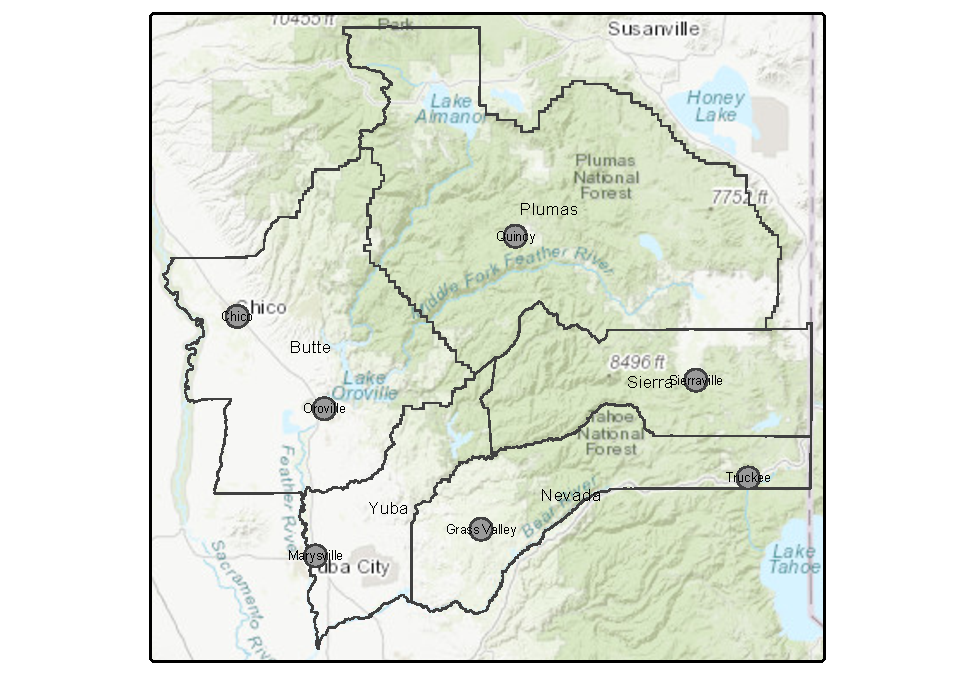
\includegraphics[width=0.75\linewidth]{EnvDataScience_files/figure-latex/spanlNSierra-1} 

}

\caption{Northern Sierra stations and places}\label{fig:spanlNSierra}
\end{figure}

So far, the above is just subsetting for a map, which may be all we're wanting to do, but we'll apply this selection to a distance function in the next section to explore a method using a reduced data set.

\subsection{Centroid}\label{centroid}

\index{centroid}Related to the topological concept of relating features inside other features is creating a new feature in the middle of an existing one, specifically a point placed in the middle of a polygon: a \emph{centroid}. Centroids are useful when you need point data for some kind of analysis, but that point needs to represent the polygon it's contained within. The methods we'll see in the code below include:

\begin{itemize}
\tightlist
\item
  \texttt{st\_centroid()} \index{st\_centroid}: to derive a single point for each tract that should be approximately in its middle. It must be topologically contained within it, not fooled by an annulus (``doughnut'') shape, for example.
\item
  \texttt{st\_make\_valid()}\index{st\_make\_valid} : to make an invalid geometry valid (or just check for it). This function has just become essential now that \texttt{sf} supports spherical instead of just planar data, which ends up containing ``slivers'' where boundaries slightly under- or overlap since they were originally built from a planar projection. The \texttt{st\_make\_valid()} appears to make minor (and typically invisible) corrections to these slivers.
\item
  \texttt{st\_bbox} \index{st\_bbox}: reads the bounding box, or spatial extent, of any dataset, which we can then use to set the scale to focus on that area. In this case, we'll focus on the census centroids instead of the statewide \texttt{CAfreeways} for instance.
\end{itemize}

Let's see the effect of the centroids and bbox. We'll start with all county centroids (Figure \ref{fig:spanlCentroids}).

\begin{Shaded}
\begin{Highlighting}[]
\FunctionTok{library}\NormalTok{(tidyverse); }\FunctionTok{library}\NormalTok{(sf); }\FunctionTok{library}\NormalTok{(igisci)}
\NormalTok{CA\_counties }\OtherTok{\textless{}{-}} \FunctionTok{st\_make\_valid}\NormalTok{(CA\_counties) }\CommentTok{\# needed fix for data}
\end{Highlighting}
\end{Shaded}

\begin{Shaded}
\begin{Highlighting}[]
\FunctionTok{ggplot}\NormalTok{() }\SpecialCharTok{+}
  \FunctionTok{geom\_sf}\NormalTok{(}\AttributeTok{data=}\NormalTok{CA\_counties) }\SpecialCharTok{+}
  \FunctionTok{geom\_sf}\NormalTok{(}\AttributeTok{data=}\FunctionTok{st\_centroid}\NormalTok{(CA\_counties))}
\end{Highlighting}
\end{Shaded}

\begin{figure}

{\centering 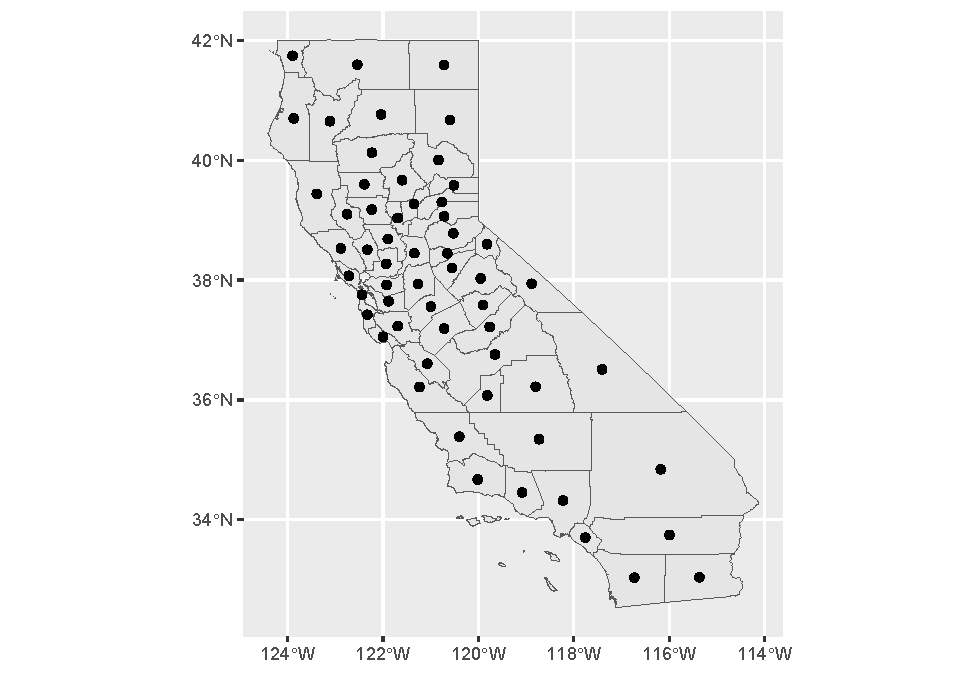
\includegraphics[width=0.75\linewidth]{EnvDataScience_files/figure-latex/spanlCentroids-1} 

}

\caption{California county centroids}\label{fig:spanlCentroids}
\end{figure}

Here's an example that also applies the \index{bbox}bounding box to establish a mapping scale that covers the Bay Area while some of the data (TRI locations and CAfreeways) are state-wide (Figure \ref{fig:spanlBayAreaTracts}).

\begin{Shaded}
\begin{Highlighting}[]
\FunctionTok{library}\NormalTok{(tidyverse)}
\FunctionTok{library}\NormalTok{(sf)}
\FunctionTok{library}\NormalTok{(igisci)}
\NormalTok{BayAreaTracts }\OtherTok{\textless{}{-}} \FunctionTok{st\_make\_valid}\NormalTok{(BayAreaTracts)}
\NormalTok{censusCentroids }\OtherTok{\textless{}{-}} \FunctionTok{st\_centroid}\NormalTok{(BayAreaTracts)}
\NormalTok{TRI\_sp }\OtherTok{\textless{}{-}} \FunctionTok{st\_as\_sf}\NormalTok{(}\FunctionTok{read\_csv}\NormalTok{(}\FunctionTok{ex}\NormalTok{(}\StringTok{"TRI/TRI\_2017\_CA.csv"}\NormalTok{)), }
                   \AttributeTok{coords =} \FunctionTok{c}\NormalTok{(}\StringTok{"LONGITUDE"}\NormalTok{, }\StringTok{"LATITUDE"}\NormalTok{), }
                   \AttributeTok{crs=}\DecValTok{4326}\NormalTok{) }\CommentTok{\# simple way to specify coordinate reference}
\NormalTok{bnd }\OtherTok{\textless{}{-}} \FunctionTok{st\_bbox}\NormalTok{(censusCentroids)}
\FunctionTok{ggplot}\NormalTok{() }\SpecialCharTok{+}
 \FunctionTok{geom\_sf}\NormalTok{(}\AttributeTok{data =}\NormalTok{ BayAreaCounties, }\FunctionTok{aes}\NormalTok{(}\AttributeTok{fill =}\NormalTok{ NAME)) }\SpecialCharTok{+}
 \FunctionTok{geom\_sf}\NormalTok{(}\AttributeTok{data =}\NormalTok{ censusCentroids) }\SpecialCharTok{+}
 \FunctionTok{geom\_sf}\NormalTok{(}\AttributeTok{data =}\NormalTok{ CAfreeways, }\AttributeTok{color =} \StringTok{"grey"}\NormalTok{, }\AttributeTok{alpha=}\FloatTok{0.5}\NormalTok{) }\SpecialCharTok{+}
 \FunctionTok{geom\_sf}\NormalTok{(}\AttributeTok{data =}\NormalTok{ TRI\_sp, }\AttributeTok{color =} \StringTok{"yellow"}\NormalTok{) }\SpecialCharTok{+}
 \FunctionTok{coord\_sf}\NormalTok{(}\AttributeTok{xlim =} \FunctionTok{c}\NormalTok{(bnd[}\DecValTok{1}\NormalTok{], bnd[}\DecValTok{3}\NormalTok{]), }\AttributeTok{ylim =} \FunctionTok{c}\NormalTok{(bnd[}\DecValTok{2}\NormalTok{], bnd[}\DecValTok{4}\NormalTok{])) }\SpecialCharTok{+}
   \FunctionTok{labs}\NormalTok{(}\AttributeTok{title=}\StringTok{"Bay Area Counties, Freeways and Census Tract Centroids"}\NormalTok{)}
\end{Highlighting}
\end{Shaded}

\begin{figure}

{\centering 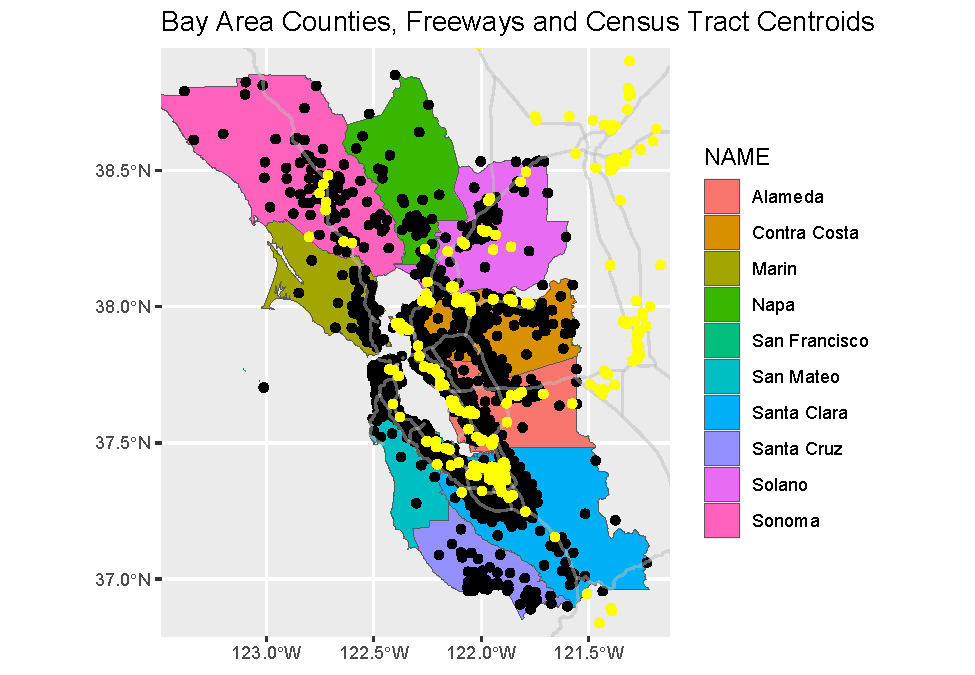
\includegraphics[width=0.75\linewidth]{EnvDataScience_files/figure-latex/spanlBayAreaTracts-1} 

}

\caption{Map scaled to cover Bay Area tracts using a bbox}\label{fig:spanlBayAreaTracts}
\end{figure}

\subsection{Distance}\label{distance}

\index{distance}Distance is a fundamental spatial measure, used to not only create spatial data (distance between points in surveying or distance to GNSS satellites) but also to analyze it. Note that we can either be referring to planar (from projected coordinate systems) or spherical (from latitude and longitude) great-circle distances. Two common spatial operations involving distance in vector spatial analysis are (a) deriving distances among features, and (b) creating buffer polygons of a specific distance away from features. In raster spatial analysis, we'll look at deriving distances from target features to each raster cell.

But first, let's take a brief excursion up the Nile River, using great circle distances to derive a longitudinal profile and channel slope\ldots{}

\subsubsection{Great circle distances}\label{great-circle-distances}

Earlier we created a simple river profile using Cartesian coordinates in metres for x, y, and z (elevation), but what if our xy locations are in geographic coordinates of latitude and longitude? Using the haversine method, we can derive great-circle (``as the crow flies'') distances between latitude and longitude pairs. The following function uses a haversine algorithm described at \url{https://www.movable-type.co.uk/scripts/latlong.html} (\emph{Calculate Distance, Bearing and More Between Latitutde/Longitude Points"} (\citeproc{ref-haversine}{n.d.})) to derive these distances in metres, provided lat/long pairs in degrees as \texttt{haversineD(lat1,lon1,lat2,lon2)}:

\begin{Shaded}
\begin{Highlighting}[]
\NormalTok{haversineD }\OtherTok{\textless{}{-}} \ControlFlowTok{function}\NormalTok{(lat1deg,lon1deg,lat2deg,lon2deg)\{}
\NormalTok{  lat1 }\OtherTok{\textless{}{-}}\NormalTok{ lat1deg}\SpecialCharTok{/}\DecValTok{180}\SpecialCharTok{*}\NormalTok{pi; lat2 }\OtherTok{\textless{}{-}}\NormalTok{ lat2deg}\SpecialCharTok{/}\DecValTok{180}\SpecialCharTok{*}\NormalTok{pi }\CommentTok{\# convert to radians}
\NormalTok{  lon1 }\OtherTok{\textless{}{-}}\NormalTok{ lon1deg}\SpecialCharTok{/}\DecValTok{180}\SpecialCharTok{*}\NormalTok{pi; lon2 }\OtherTok{\textless{}{-}}\NormalTok{ lon2deg}\SpecialCharTok{/}\DecValTok{180}\SpecialCharTok{*}\NormalTok{pi}
\NormalTok{  a }\OtherTok{\textless{}{-}} \FunctionTok{sin}\NormalTok{((lat2}\SpecialCharTok{{-}}\NormalTok{lat1)}\SpecialCharTok{/}\DecValTok{2}\NormalTok{)}\SpecialCharTok{\^{}}\DecValTok{2} \SpecialCharTok{+} \FunctionTok{cos}\NormalTok{(lat1)}\SpecialCharTok{*}\FunctionTok{cos}\NormalTok{(lat2)}\SpecialCharTok{*}\FunctionTok{sin}\NormalTok{((lon2}\SpecialCharTok{{-}}\NormalTok{lon1)}\SpecialCharTok{/}\DecValTok{2}\NormalTok{)}\SpecialCharTok{\^{}}\DecValTok{2}
\NormalTok{  c }\OtherTok{\textless{}{-}} \DecValTok{2}\SpecialCharTok{*}\FunctionTok{atan2}\NormalTok{(}\FunctionTok{sqrt}\NormalTok{(a),}\FunctionTok{sqrt}\NormalTok{(}\DecValTok{1}\SpecialCharTok{{-}}\NormalTok{a))}
\NormalTok{  c }\SpecialCharTok{*} \FloatTok{6.371e6} \CommentTok{\# mean earth radius is \textasciitilde{} 6.371 million metres}
\NormalTok{\}}
\end{Highlighting}
\end{Shaded}

We'll use these to help us derived channel slope where we need the longitudinal distance in metres along the Nile River, but we have locations in geographic coordinates (crs 4326). But first, here's a few quick checks on the function since I remember that 1 minute (1/60 degree) of latitude is equal to 1 nautical mile (NM) or \textasciitilde1.15 statute miles, and the same applies to longitude at the equator. Then longitude is half that at 60 degrees north or south.

\begin{Shaded}
\begin{Highlighting}[]
\FunctionTok{paste}\NormalTok{(}\StringTok{"1\textquotesingle{}lat="}\NormalTok{,}\FunctionTok{haversineD}\NormalTok{(}\DecValTok{30}\NormalTok{,}\DecValTok{120}\NormalTok{,}\DecValTok{30}\SpecialCharTok{+}\DecValTok{1}\SpecialCharTok{/}\DecValTok{60}\NormalTok{,}\DecValTok{120}\NormalTok{)}\SpecialCharTok{/}\FloatTok{0.3048}\SpecialCharTok{/}\DecValTok{5280}\NormalTok{,}\StringTok{"miles at 30°N"}\NormalTok{)}
\FunctionTok{paste}\NormalTok{(}\StringTok{"1\textquotesingle{}lat="}\NormalTok{,}\FunctionTok{haversineD}\NormalTok{(}\DecValTok{30}\NormalTok{,}\DecValTok{120}\NormalTok{,}\DecValTok{30}\SpecialCharTok{+}\DecValTok{1}\SpecialCharTok{/}\DecValTok{60}\NormalTok{,}\DecValTok{120}\NormalTok{)}\SpecialCharTok{/}\FloatTok{0.3048}\SpecialCharTok{/}\DecValTok{6076}\NormalTok{,}\StringTok{"NM at 30°N"}\NormalTok{)}
\FunctionTok{paste}\NormalTok{(}\StringTok{"1\textquotesingle{}lon="}\NormalTok{,}\FunctionTok{haversineD}\NormalTok{(}\DecValTok{0}\NormalTok{,}\DecValTok{0}\NormalTok{,}\DecValTok{0}\NormalTok{,}\DecValTok{1}\SpecialCharTok{/}\DecValTok{60}\NormalTok{)}\SpecialCharTok{/}\FloatTok{0.3048}\SpecialCharTok{/}\DecValTok{6076}\NormalTok{,}\StringTok{"NM at the equator"}\NormalTok{)}
\FunctionTok{paste}\NormalTok{(}\StringTok{"1\textquotesingle{}lon="}\NormalTok{,}\FunctionTok{haversineD}\NormalTok{(}\DecValTok{60}\NormalTok{,}\DecValTok{0}\NormalTok{,}\DecValTok{60}\NormalTok{,}\DecValTok{1}\SpecialCharTok{/}\DecValTok{60}\NormalTok{)}\SpecialCharTok{/}\FloatTok{0.3048}\SpecialCharTok{/}\DecValTok{6076}\NormalTok{,}\StringTok{"NM at 60°N"}\NormalTok{)}
\end{Highlighting}
\end{Shaded}

\begin{verbatim}
## [1] "1'lat= 1.15155540233128 miles at 30°N"
## [1] "1'lat= 1.000693305515 NM at 30°N"
## [1] "1'lon= 1.00069330551494 NM at the equator"
## [1] "1'lon= 0.500346651434429 NM at 60°N"
\end{verbatim}

Thanks to Stephanie Kate in my Fall 2020 Environmental Data Science course at SFSU, we have geographic coordinates and elevations in metres for a series of points along the Nile River, including various tributaries. We'll focus on the main to Blue Nile and generate a map (Figure \ref{fig:spanlNileMap}) and longitudinal profile (Figure \ref{fig:spanlNileLong}), using great circle distances along the channel.

\begin{Shaded}
\begin{Highlighting}[]
\FunctionTok{library}\NormalTok{(igisci); }\FunctionTok{library}\NormalTok{(tidyverse)}
\NormalTok{bNile }\OtherTok{\textless{}{-}} \FunctionTok{read\_csv}\NormalTok{(}\FunctionTok{ex}\NormalTok{(}\StringTok{"Nile/NilePoints.csv"}\NormalTok{)) }\SpecialCharTok{\%\textgreater{}\%} 
  \FunctionTok{filter}\NormalTok{(nile }\SpecialCharTok{\%in\%} \FunctionTok{c}\NormalTok{(}\StringTok{"main"}\NormalTok{,}\StringTok{"blue"}\NormalTok{)) }\SpecialCharTok{\%\textgreater{}\%}
  \FunctionTok{arrange}\NormalTok{(elev\_meter) }\SpecialCharTok{\%\textgreater{}\%}
  \FunctionTok{mutate}\NormalTok{(}\AttributeTok{d=}\DecValTok{0}\NormalTok{, }\AttributeTok{longd=}\DecValTok{0}\NormalTok{, }\AttributeTok{s=}\FloatTok{1e{-}6}\NormalTok{) }\CommentTok{\# initiate distance, longitudinal distance \& slope}
\FunctionTok{tmap\_mode}\NormalTok{(}\StringTok{"plot"}\NormalTok{)}
\end{Highlighting}
\end{Shaded}

\begin{Shaded}
\begin{Highlighting}[]
\ControlFlowTok{for}\NormalTok{(i }\ControlFlowTok{in} \DecValTok{2}\SpecialCharTok{:}\FunctionTok{length}\NormalTok{(bNile}\SpecialCharTok{$}\NormalTok{x))\{}
\NormalTok{  bNile}\SpecialCharTok{$}\NormalTok{d[i] }\OtherTok{\textless{}{-}} \FunctionTok{haversineD}\NormalTok{(bNile}\SpecialCharTok{$}\NormalTok{y[i],bNile}\SpecialCharTok{$}\NormalTok{x[i],bNile}\SpecialCharTok{$}\NormalTok{y[i}\DecValTok{{-}1}\NormalTok{],bNile}\SpecialCharTok{$}\NormalTok{x[i}\DecValTok{{-}1}\NormalTok{])}
\NormalTok{  bNile}\SpecialCharTok{$}\NormalTok{longd[i] }\OtherTok{\textless{}{-}}\NormalTok{ bNile}\SpecialCharTok{$}\NormalTok{longd[i}\DecValTok{{-}1}\NormalTok{] }\SpecialCharTok{+}\NormalTok{ bNile}\SpecialCharTok{$}\NormalTok{d[i]}
\NormalTok{  bNile}\SpecialCharTok{$}\NormalTok{s[i}\DecValTok{{-}1}\NormalTok{] }\OtherTok{\textless{}{-}}\NormalTok{ (bNile}\SpecialCharTok{$}\NormalTok{elev\_meter[i]}\SpecialCharTok{{-}}\NormalTok{bNile}\SpecialCharTok{$}\NormalTok{elev\_meter[i}\DecValTok{{-}1}\NormalTok{])}\SpecialCharTok{/}\NormalTok{bNile}\SpecialCharTok{$}\NormalTok{d[i]}
\NormalTok{\}}
\end{Highlighting}
\end{Shaded}

\begin{Shaded}
\begin{Highlighting}[]
\FunctionTok{library}\NormalTok{(sf); }\FunctionTok{library}\NormalTok{(tmap); }\FunctionTok{library}\NormalTok{(maptiles); }\FunctionTok{library}\NormalTok{(tmaptools)}
\NormalTok{Nile\_sf }\OtherTok{\textless{}{-}} \FunctionTok{st\_as\_sf}\NormalTok{(bNile,}\AttributeTok{coords=}\FunctionTok{c}\NormalTok{(}\StringTok{"x"}\NormalTok{,}\StringTok{"y"}\NormalTok{),}\AttributeTok{crs=}\DecValTok{4326}\NormalTok{) }\SpecialCharTok{|\textgreater{}}
  \FunctionTok{mutate}\NormalTok{(}\AttributeTok{s\_pct =}\NormalTok{ s}\SpecialCharTok{*}\DecValTok{100}\NormalTok{)}
\FunctionTok{tm\_basemap}\NormalTok{(}\AttributeTok{server =}\StringTok{"Esri.NatGeoWorldMap"}\NormalTok{) }\SpecialCharTok{+}
  \FunctionTok{tm\_graticules}\NormalTok{(}\AttributeTok{alpha=}\FloatTok{0.5}\NormalTok{) }\SpecialCharTok{+} 
  \FunctionTok{tm\_shape}\NormalTok{(Nile\_sf) }\SpecialCharTok{+}
    \FunctionTok{tm\_dots}\NormalTok{(}\AttributeTok{size=}\FloatTok{0.3}\NormalTok{, }\AttributeTok{fill=}\StringTok{"elev\_meter"}\NormalTok{,}
            \AttributeTok{fill.scale=}\FunctionTok{tm\_scale\_continuous}\NormalTok{(}\AttributeTok{values=}\StringTok{"brewer.yl\_or\_rd"}\NormalTok{),}
            \AttributeTok{fill.legend=}\FunctionTok{tm\_legend}\NormalTok{(}\AttributeTok{reverse=}\NormalTok{T, }\AttributeTok{frame=}\NormalTok{F))}
\end{Highlighting}
\end{Shaded}

\begin{figure}

{\centering 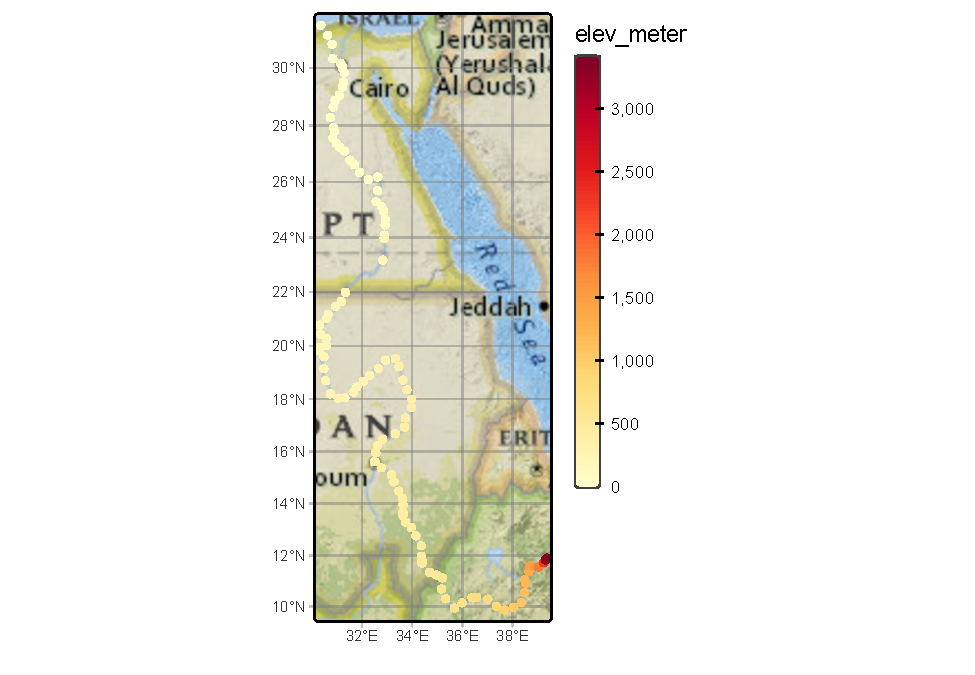
\includegraphics[width=0.75\linewidth]{EnvDataScience_files/figure-latex/spanlNileMap-1} 

}

\caption{Nile River points, colored by channel slope}\label{fig:spanlNileMap}
\end{figure}

\begin{Shaded}
\begin{Highlighting}[]
\FunctionTok{ggplot}\NormalTok{(bNile, }\FunctionTok{aes}\NormalTok{(longd,elev\_meter)) }\SpecialCharTok{+} \FunctionTok{geom\_line}\NormalTok{(}\FunctionTok{aes}\NormalTok{(}\AttributeTok{col=}\NormalTok{s), }\AttributeTok{linewidth=}\FloatTok{1.5}\NormalTok{) }\SpecialCharTok{+}
  \FunctionTok{scale\_color\_gradient}\NormalTok{(}\AttributeTok{low=}\StringTok{"green"}\NormalTok{, }\AttributeTok{high=}\StringTok{"red"}\NormalTok{) }\SpecialCharTok{+}
  \FunctionTok{ggtitle}\NormalTok{(}\StringTok{"Nile River to Blue Nile longitudinal profile"}\NormalTok{)}
\end{Highlighting}
\end{Shaded}

\begin{figure}

{\centering 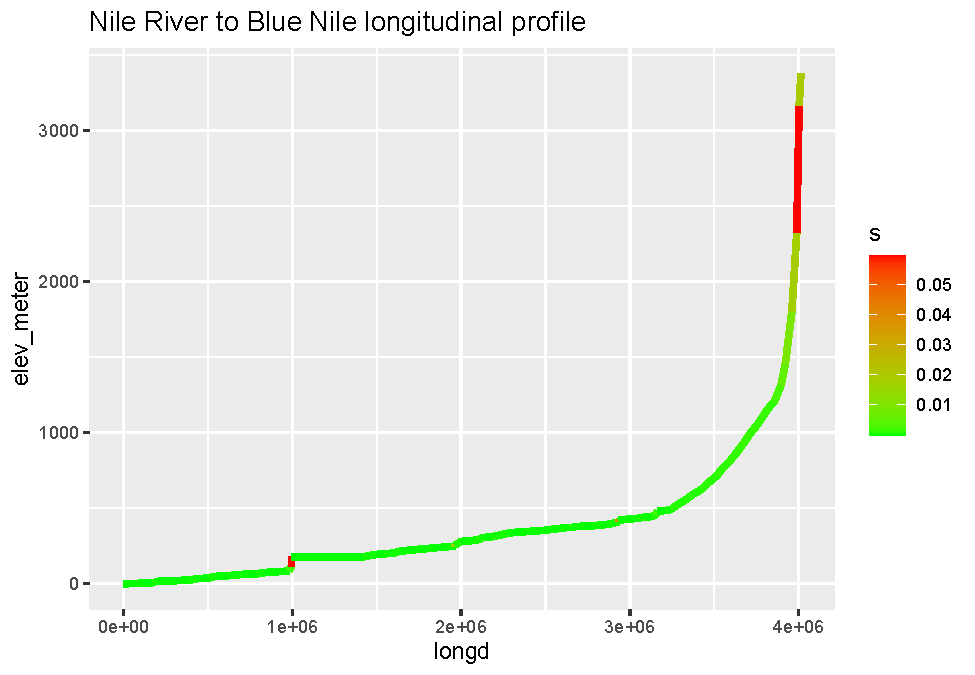
\includegraphics[width=0.75\linewidth]{EnvDataScience_files/figure-latex/spanlNileLong-1} 

}

\caption{Nile River channel slope as range of colors from green to red, with great circle channel distances derived using the haversine method}\label{fig:spanlNileLong}
\end{figure}

\subsubsection{Distances among features}\label{distances-among-features}

\index{distance among features}The sf \texttt{st\_distance} and terra \texttt{distance} functions derive distances between features, either among features of one data set object or between all features in one and all features in another data set.

To see how this works, we'll look at a purposefully small dataset: a selection of Marble Mountains soil CO\textsubscript{2} sampling sites and in-cave water quality sampling sites. We'll start by reading in the data, and filtering to just get cave water samples and a small set of nearby soil CO\textsubscript{2} sampling sites:

\begin{Shaded}
\begin{Highlighting}[]
\FunctionTok{library}\NormalTok{(igisci); }\FunctionTok{library}\NormalTok{(sf); }\FunctionTok{library}\NormalTok{(tidyverse)}
\NormalTok{soilCO2all }\OtherTok{\textless{}{-}} \FunctionTok{st\_read}\NormalTok{(}\FunctionTok{ex}\NormalTok{(}\StringTok{"marbles/co2july95.shp"}\NormalTok{))}
\NormalTok{cave\_H2Osamples }\OtherTok{\textless{}{-}} \FunctionTok{st\_read}\NormalTok{(}\FunctionTok{ex}\NormalTok{(}\StringTok{"marbles/samples.shp"}\NormalTok{)) }\SpecialCharTok{\%\textgreater{}\%}
  \FunctionTok{filter}\NormalTok{((SAMPLES\_ID }\SpecialCharTok{\textgreater{}=} \DecValTok{50}\NormalTok{) }\SpecialCharTok{\&}\NormalTok{ (SAMPLES\_ID }\SpecialCharTok{\textless{}} \DecValTok{60}\NormalTok{)) }\CommentTok{\# these are the cave samples}
\NormalTok{soilCO2 }\OtherTok{\textless{}{-}}\NormalTok{ soilCO2all }\SpecialCharTok{\%\textgreater{}\%} \FunctionTok{filter}\NormalTok{(LOC }\SpecialCharTok{\textgreater{}} \DecValTok{20}\NormalTok{) }\CommentTok{\# soil CO2 samples in the area}
\end{Highlighting}
\end{Shaded}

Figure \ref{fig:spanlSelSoilCO2} shows the six selected soil CO\textsubscript{2} samples.

\begin{Shaded}
\begin{Highlighting}[]
\FunctionTok{library}\NormalTok{(tmap); }\FunctionTok{library}\NormalTok{(maptiles)}
\FunctionTok{tmap\_mode}\NormalTok{(}\StringTok{"plot"}\NormalTok{)}
\NormalTok{bbox }\OtherTok{\textless{}{-}}\NormalTok{ tmaptools}\SpecialCharTok{::}\FunctionTok{bb}\NormalTok{(soilCO2, }\AttributeTok{ext=}\FloatTok{1.1}\NormalTok{) }\CommentTok{\# extends the map area a bit from the points}
\FunctionTok{tm\_basemap}\NormalTok{(}\AttributeTok{server=}\StringTok{"OpenTopoMap"}\NormalTok{) }\SpecialCharTok{+} \FunctionTok{tm\_graticules}\NormalTok{(}\AttributeTok{alpha=}\FloatTok{0.5}\NormalTok{) }\SpecialCharTok{+} 
  \FunctionTok{tm\_shape}\NormalTok{(soilCO2, }\AttributeTok{bbox=}\NormalTok{bbox) }\SpecialCharTok{+} 
    \FunctionTok{tm\_symbols}\NormalTok{(}\AttributeTok{fill=}\StringTok{"CO2\_"}\NormalTok{, }\AttributeTok{fill.scale=}\FunctionTok{tm\_scale\_continuous}\NormalTok{(}\AttributeTok{values=}\StringTok{"parks.denali"}\NormalTok{),}
               \AttributeTok{fill.legend=}\FunctionTok{tm\_legend}\NormalTok{(}\AttributeTok{frame=}\NormalTok{F)) }\SpecialCharTok{+}
  \FunctionTok{tm\_shape}\NormalTok{(soilCO2) }\SpecialCharTok{+} \FunctionTok{tm\_text}\NormalTok{(}\StringTok{"LOC"}\NormalTok{, }\AttributeTok{size=}\FloatTok{0.5}\NormalTok{, }\AttributeTok{col=}\StringTok{"orange"}\NormalTok{)}
\end{Highlighting}
\end{Shaded}

\begin{figure}

{\centering 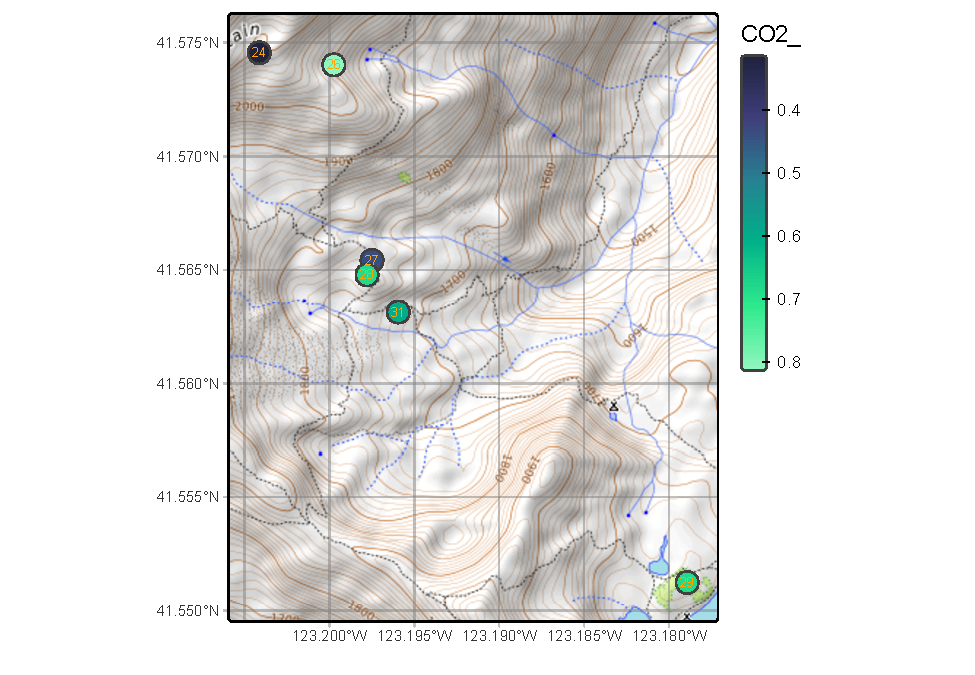
\includegraphics[width=0.75\linewidth]{EnvDataScience_files/figure-latex/spanlSelSoilCO2-1} 

}

\caption{Selection of soil CO2 sampling sites, July 1995}\label{fig:spanlSelSoilCO2}
\end{figure}

If you just provide the six soil CO\textsubscript{2} sample points as a single feature data set input to the st\_distance function, it returns a matrix of distances between each, with a diagonal of zeros where the distance would be to itself:

\begin{Shaded}
\begin{Highlighting}[]
\FunctionTok{st\_distance}\NormalTok{(soilCO2)}
\end{Highlighting}
\end{Shaded}

\begin{verbatim}
## Units: [m]
##           1         2          3          4        5         6
## 1    0.0000  370.5894 1155.64981 1207.62172 3333.529 1439.2366
## 2  370.5894    0.0000  973.73559 1039.45041 3067.106 1248.9347
## 3 1155.6498  973.7356    0.00000   75.14093 2207.019  283.6722
## 4 1207.6217 1039.4504   75.14093    0.00000 2174.493  237.7024
## 5 3333.5290 3067.1061 2207.01903 2174.49276    0.000 1938.2985
## 6 1439.2366 1248.9347  283.67215  237.70236 1938.299    0.0000
\end{verbatim}

Then we'll look at \index{distances}distances between this same set of soil CO\textsubscript{2} samples with water samples collected in caves, where the effect of elevated soil CO\textsubscript{2} values might influence solution processes reflected in cave waters (Figure \ref{fig:spanlSoilH2O}).

\begin{Shaded}
\begin{Highlighting}[]
\FunctionTok{library}\NormalTok{(tmap)}
\FunctionTok{tmap\_mode}\NormalTok{(}\StringTok{"plot"}\NormalTok{)}
\NormalTok{bbox }\OtherTok{\textless{}{-}}\NormalTok{ tmaptools}\SpecialCharTok{::}\FunctionTok{bb}\NormalTok{(}\FunctionTok{st\_union}\NormalTok{(cave\_H2Osamples, soilCO2),}\AttributeTok{ext=}\FloatTok{1.1}\NormalTok{)}
\FunctionTok{tm\_basemap}\NormalTok{(}\StringTok{"OpenTopoMap"}\NormalTok{) }\SpecialCharTok{+} \CommentTok{\#tm\_graticules() +}
  \FunctionTok{tm\_shape}\NormalTok{(cave\_H2Osamples, }\AttributeTok{bbox=}\NormalTok{bbox) }\SpecialCharTok{+} 
    \FunctionTok{tm\_symbols}\NormalTok{(}\AttributeTok{fill=}\StringTok{"CATOT"}\NormalTok{, }\AttributeTok{fill.scale=}\FunctionTok{tm\_scale\_continuous}\NormalTok{(}\AttributeTok{values=}\StringTok{"brewer.blues"}\NormalTok{),}
               \AttributeTok{fill.legend=}\FunctionTok{tm\_legend}\NormalTok{(}\AttributeTok{frame=}\NormalTok{F))}\SpecialCharTok{+} 
  \FunctionTok{tm\_shape}\NormalTok{(soilCO2) }\SpecialCharTok{+}
    \FunctionTok{tm\_symbols}\NormalTok{(}\AttributeTok{fill=}\StringTok{"CO2\_"}\NormalTok{,  }\AttributeTok{fill.scale=}\FunctionTok{tm\_scale\_continuous}\NormalTok{(}\AttributeTok{values=}\StringTok{"brewer.reds"}\NormalTok{),}
                             \AttributeTok{fill.legend=}\FunctionTok{tm\_legend}\NormalTok{(}\AttributeTok{frame=}\NormalTok{F))}
\end{Highlighting}
\end{Shaded}

\begin{figure}

{\centering 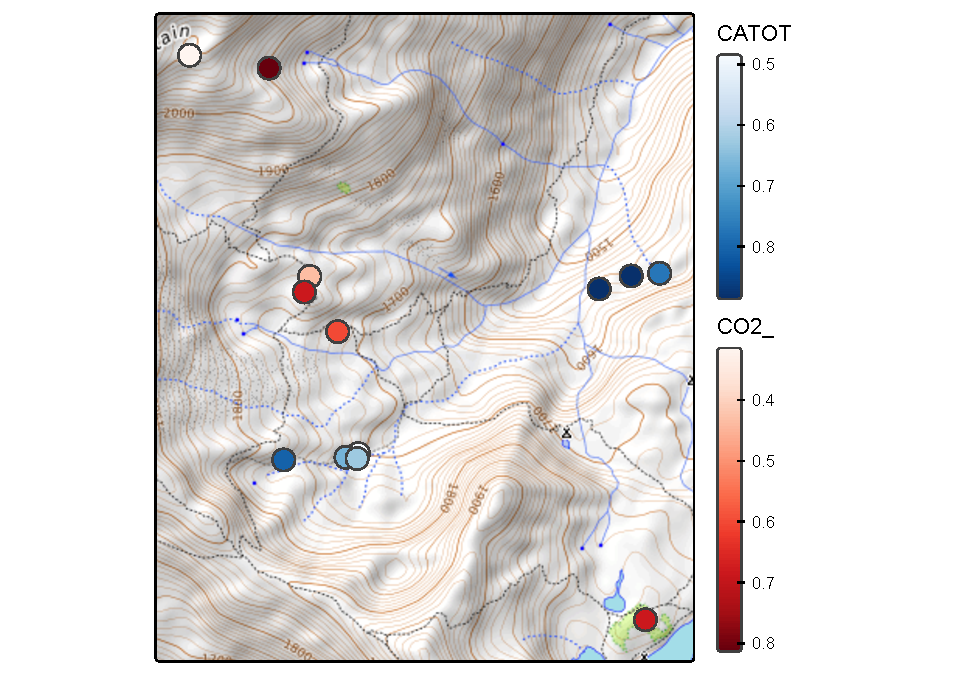
\includegraphics[width=0.75\linewidth]{EnvDataScience_files/figure-latex/spanlSoilH2O-1} 

}

\caption{Selection of soil CO2 and in-cave water samples}\label{fig:spanlSoilH2O}
\end{figure}

\begin{Shaded}
\begin{Highlighting}[]
\NormalTok{soilwater }\OtherTok{\textless{}{-}} \FunctionTok{st\_distance}\NormalTok{(soilCO2, cave\_H2Osamples)}
\NormalTok{soilwater}
\end{Highlighting}
\end{Shaded}

\begin{verbatim}
## Units: [m]
##          [,1]     [,2]     [,3]      [,4]      [,5]      [,6]      [,7]
## [1,] 2384.210 2271.521 2169.301 1985.6093 1980.0314 2004.1697 1905.9543
## [2,] 2029.748 1920.783 1826.579 1815.2653 1820.0496 1835.9465 1798.1216
## [3,] 1611.381 1480.688 1334.287  842.8228  846.3210  863.1026  849.7313
## [4,] 1637.998 1506.938 1357.582  781.9741  782.4215  801.6262  776.0732
## [5,] 1590.469 1578.730 1532.465 1526.3315 1567.5677 1520.1399 1820.3651
## [6,] 1506.358 1375.757 1220.000  567.8210  578.1919  589.1443  638.8615
\end{verbatim}

In this case, the six soil CO\textsubscript{2} samples are the rows, and the seven cave water sample locations are the columns. We aren't really relating the values but just looking at distances. An analysis of this data might not be very informative because the caves aren't very near the soil samples, and conduit cave hydrology doesn't lend itself to looking at euclidean distance, but the purpose of this example is just to comprehend the results of the \texttt{sf::st\_distance} or similarly the \texttt{terra::distance} function.

\subsubsection{Distance to the nearest feature, abstracted from distance matrix}\label{distance-to-the-nearest-feature-abstracted-from-distance-matrix}

\index{distance to the nearest feature}However, let's process the matrix a bit to find the distance from each soil CO\textsubscript{2} sample to the closest cave water sample:

\begin{Shaded}
\begin{Highlighting}[]
\NormalTok{soilCO2d }\OtherTok{\textless{}{-}}\NormalTok{ soilCO2 }\SpecialCharTok{\%\textgreater{}\%} \FunctionTok{mutate}\NormalTok{(}\AttributeTok{dist2cave =} \FunctionTok{min}\NormalTok{(soilwater[}\DecValTok{1}\NormalTok{,]))}
\ControlFlowTok{for}\NormalTok{ (i }\ControlFlowTok{in} \DecValTok{1}\SpecialCharTok{:}\FunctionTok{length}\NormalTok{(soilwater[,}\DecValTok{1}\NormalTok{])) soilCO2d[i,}\StringTok{"dist2cave"}\NormalTok{] }\OtherTok{\textless{}{-}} \FunctionTok{min}\NormalTok{(soilwater[i,])}
\NormalTok{soilCO2d }\SpecialCharTok{\%\textgreater{}\%}\NormalTok{ dplyr}\SpecialCharTok{::}\FunctionTok{select}\NormalTok{(DESCRIPTIO, dist2cave) }\SpecialCharTok{\%\textgreater{}\%} \FunctionTok{st\_set\_geometry}\NormalTok{(}\ConstantTok{NULL}\NormalTok{)}
\end{Highlighting}
\end{Shaded}

\begin{verbatim}
##                                              DESCRIPTIO     dist2cave
## 1                Super Sink moraine, low point W of 241 1905.9543 [m]
## 2      Small sink, first in string on hike to SuperSink 1798.1216 [m]
## 3        meadow on bench above Mbl Valley, 25' E of PCT  842.8228 [m]
## 4        red fir forest S of upper meadow, 30' W of PCT  776.0732 [m]
## 5            saddle betw Lower Skyhigh (E) & Frying Pan 1520.1399 [m]
## 6 E end of wide soil-filled 10m fissure N of lower camp  567.8210 [m]
\end{verbatim}

\ldots{} or since we can also look at distances to lines or polygons, we can find the distance from CO\textsubscript{2} sampling locations to the closest stream (Figure \ref{fig:spanlDistCO2streams}),

\begin{Shaded}
\begin{Highlighting}[]
\FunctionTok{library}\NormalTok{(igisci); }\FunctionTok{library}\NormalTok{(sf); }\FunctionTok{library}\NormalTok{(tidyverse)}
\NormalTok{soilCO2all }\OtherTok{\textless{}{-}} \FunctionTok{st\_read}\NormalTok{(}\FunctionTok{ex}\NormalTok{(}\StringTok{"marbles/co2july95.shp"}\NormalTok{))}
\NormalTok{streams }\OtherTok{\textless{}{-}} \FunctionTok{st\_read}\NormalTok{(}\FunctionTok{ex}\NormalTok{(}\StringTok{"marbles/streams.shp"}\NormalTok{))}
\end{Highlighting}
\end{Shaded}

\begin{Shaded}
\begin{Highlighting}[]
\NormalTok{strCO2 }\OtherTok{\textless{}{-}} \FunctionTok{st\_distance}\NormalTok{(soilCO2all, streams)}
\NormalTok{strCO2d }\OtherTok{\textless{}{-}}\NormalTok{ soilCO2all }\SpecialCharTok{\%\textgreater{}\%} \FunctionTok{mutate}\NormalTok{(}\AttributeTok{dist2stream =} \FunctionTok{min}\NormalTok{(strCO2[}\DecValTok{1}\NormalTok{,]))}
\ControlFlowTok{for}\NormalTok{ (i }\ControlFlowTok{in} \DecValTok{1}\SpecialCharTok{:}\FunctionTok{length}\NormalTok{(strCO2[,}\DecValTok{1}\NormalTok{])) strCO2d[i,}\StringTok{"dist2stream"}\NormalTok{] }\OtherTok{\textless{}{-}} \FunctionTok{min}\NormalTok{(strCO2[i,])}
\end{Highlighting}
\end{Shaded}

\begin{Shaded}
\begin{Highlighting}[]
\FunctionTok{tm\_basemap}\NormalTok{(}\StringTok{"OpenTopoMap"}\NormalTok{) }\SpecialCharTok{+} \FunctionTok{tm\_graticules}\NormalTok{() }\SpecialCharTok{+} 
  \FunctionTok{tm\_shape}\NormalTok{(streams) }\SpecialCharTok{+} \FunctionTok{tm\_lines}\NormalTok{(}\AttributeTok{col=}\StringTok{"blue"}\NormalTok{) }\SpecialCharTok{+}
  \FunctionTok{tm\_shape}\NormalTok{(strCO2d) }\SpecialCharTok{+} \FunctionTok{tm\_symbols}\NormalTok{(}\AttributeTok{fill=}\StringTok{"dist2stream"}\NormalTok{,}
                                \AttributeTok{fill.legend=}\FunctionTok{tm\_legend}\NormalTok{(}\AttributeTok{frame=}\NormalTok{F)) }
\end{Highlighting}
\end{Shaded}

\begin{figure}

{\centering 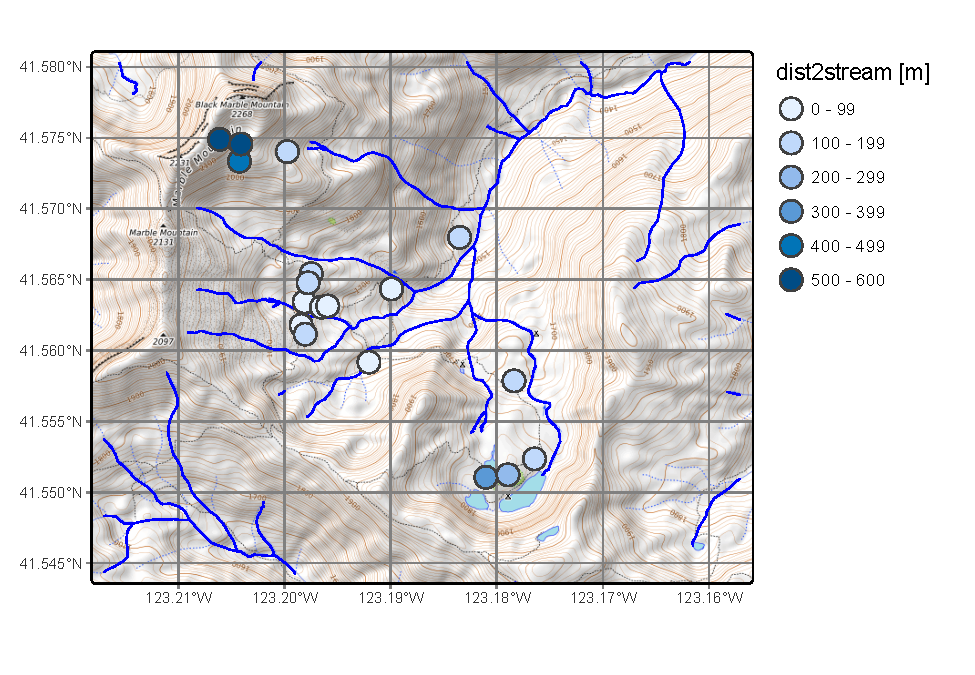
\includegraphics[width=0.75\linewidth]{EnvDataScience_files/figure-latex/spanlDistCO2streams-1} 

}

\caption{Distance from CO2 samples to closest streams (not including lakes)}\label{fig:spanlDistCO2streams}
\end{figure}

\subsubsection{Nearest feature detection}\label{nearest-feature-detection}

\index{nearest feature detection}As we just saw, the matrix derived from \texttt{st\_distance} when applied to feature data sets could be used for further analyses, such as this distance to the nearest place. But there's another approach to this using a specific function that identifies the nearest feature: \index{st\_nearest\_feature}\texttt{st\_nearest\_feature}, so we'll look at this with the previously filtered northern Sierra places and weather stations. We start by using \texttt{st\_nearest\_feature} to create an index vector of the nearest place to each station, and grab its location geometry:

\begin{Shaded}
\begin{Highlighting}[]
\NormalTok{nearest\_Place }\OtherTok{\textless{}{-}} \FunctionTok{st\_nearest\_feature}\NormalTok{(nSierraStations, nSierraPlaces)}
\NormalTok{near\_Place\_loc }\OtherTok{\textless{}{-}}\NormalTok{ nSierraPlaces}\SpecialCharTok{$}\NormalTok{geometry[nearest\_Place]}
\end{Highlighting}
\end{Shaded}

Then add the distance to that nearest place to our \texttt{nSierraStations} \texttt{sf}. Note that we're using \texttt{st\_distance} with two vector inputs as before, but ending up with just one distance per feature (instead of a matrix) with the setting \texttt{by\_element=TRUE}\ldots{}

\begin{Shaded}
\begin{Highlighting}[]
\NormalTok{nSierraStations }\OtherTok{\textless{}{-}}\NormalTok{ nSierraStations }\SpecialCharTok{\%\textgreater{}\%}
  \FunctionTok{mutate}\NormalTok{(}\AttributeTok{d2Place =} \FunctionTok{st\_distance}\NormalTok{(nSierraStations, near\_Place\_loc, }\AttributeTok{by\_element=}\ConstantTok{TRUE}\NormalTok{),}
         \AttributeTok{d2Place =}\NormalTok{ units}\SpecialCharTok{::}\FunctionTok{drop\_units}\NormalTok{(d2Place))}
\end{Highlighting}
\end{Shaded}

\ldots{} and of course map the results (Figure \ref{fig:spanlDistStations}):

\begin{Shaded}
\begin{Highlighting}[]
\FunctionTok{tm\_basemap}\NormalTok{(}\StringTok{"OpenStreetMap"}\NormalTok{) }\SpecialCharTok{+} \FunctionTok{tm\_graticules}\NormalTok{(}\AttributeTok{alpha=}\FloatTok{0.5}\NormalTok{) }\SpecialCharTok{+} 
  \FunctionTok{tm\_shape}\NormalTok{(nSierraCo) }\SpecialCharTok{+} \FunctionTok{tm\_borders}\NormalTok{() }\SpecialCharTok{+} \FunctionTok{tm\_text}\NormalTok{(}\StringTok{"NAME"}\NormalTok{) }\SpecialCharTok{+}
  \FunctionTok{tm\_shape}\NormalTok{(nSierraStations) }\SpecialCharTok{+} \FunctionTok{tm\_symbols}\NormalTok{(}\AttributeTok{fill=}\StringTok{"d2Place"}\NormalTok{) }\SpecialCharTok{+}
  \FunctionTok{tm\_shape}\NormalTok{(nSierraPlaces) }\SpecialCharTok{+} \FunctionTok{tm\_symbols}\NormalTok{(}\AttributeTok{fill=}\StringTok{"red"}\NormalTok{, }\AttributeTok{fill\_alpha=}\FloatTok{0.5}\NormalTok{, }\AttributeTok{size=}\FloatTok{0.5}\NormalTok{, }\AttributeTok{shape=}\DecValTok{24}\NormalTok{,}
                                      \AttributeTok{fill.legend=}\FunctionTok{tm\_legend}\NormalTok{(}\AttributeTok{frame=}\NormalTok{F))}
\end{Highlighting}
\end{Shaded}

\begin{figure}

{\centering 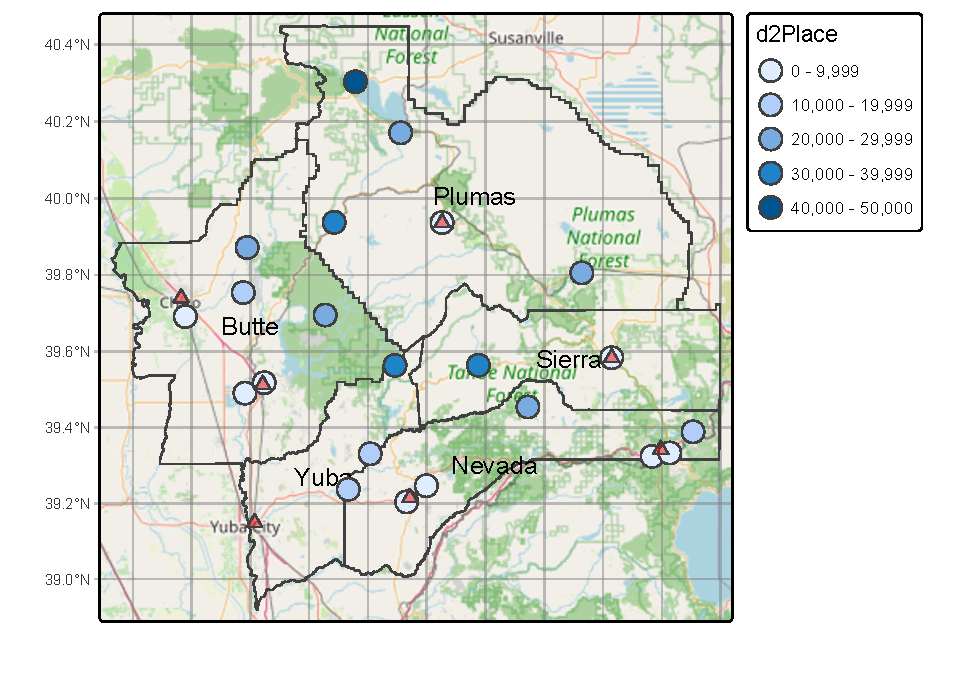
\includegraphics[width=0.75\linewidth]{EnvDataScience_files/figure-latex/spanlDistStations-1} 

}

\caption{Distance to towns (places) from weather stations}\label{fig:spanlDistStations}
\end{figure}

That's probably enough examples of using distance to nearest feature so we can see how it works, but to see an example with a larger data set, an example in \textbf{Appendix A7.2} looks at the proximity of TRI sites to health data at census tracts.

\subsection{Buffers}\label{buffers}

\index{buffers}Creating buffers, or polygons defining the area within some distance of a feature, is commonly used in GIS. Since you need to specify that distance (or read it from a variable for each feature), you need to know what the horizontal distance units are for your data. If GCS, these will be decimal degrees and 1 degree is a long way, about 111 km (or 69 miles), though that differs for longitude where 1 degree of longitude is 111 km * cos(latitude). If in UTM, the horizontal distance will be in metres, but in the US, state plane coordinates are typically in feet. So let's read the trails shapefile from the Marble Mountains and look for its units:

\begin{Shaded}
\begin{Highlighting}[]
\FunctionTok{library}\NormalTok{(igisci)}
\FunctionTok{library}\NormalTok{(sf); }\FunctionTok{library}\NormalTok{(tidyverse)}
\NormalTok{trails }\OtherTok{\textless{}{-}} \FunctionTok{st\_read}\NormalTok{(}\FunctionTok{ex}\NormalTok{(}\StringTok{"marbles/trails.shp"}\NormalTok{))}
\end{Highlighting}
\end{Shaded}

Then we know we're in metres, so we'll create a 100 m buffer this way (Figure \ref{fig:spanlTrailBuffer}).

\begin{Shaded}
\begin{Highlighting}[]
\NormalTok{trail\_buff0 }\OtherTok{\textless{}{-}} \FunctionTok{st\_buffer}\NormalTok{(trails,}\DecValTok{100}\NormalTok{)}
\FunctionTok{ggplot}\NormalTok{(trail\_buff0) }\SpecialCharTok{+} \FunctionTok{geom\_sf}\NormalTok{()}
\end{Highlighting}
\end{Shaded}

\begin{figure}

{\centering 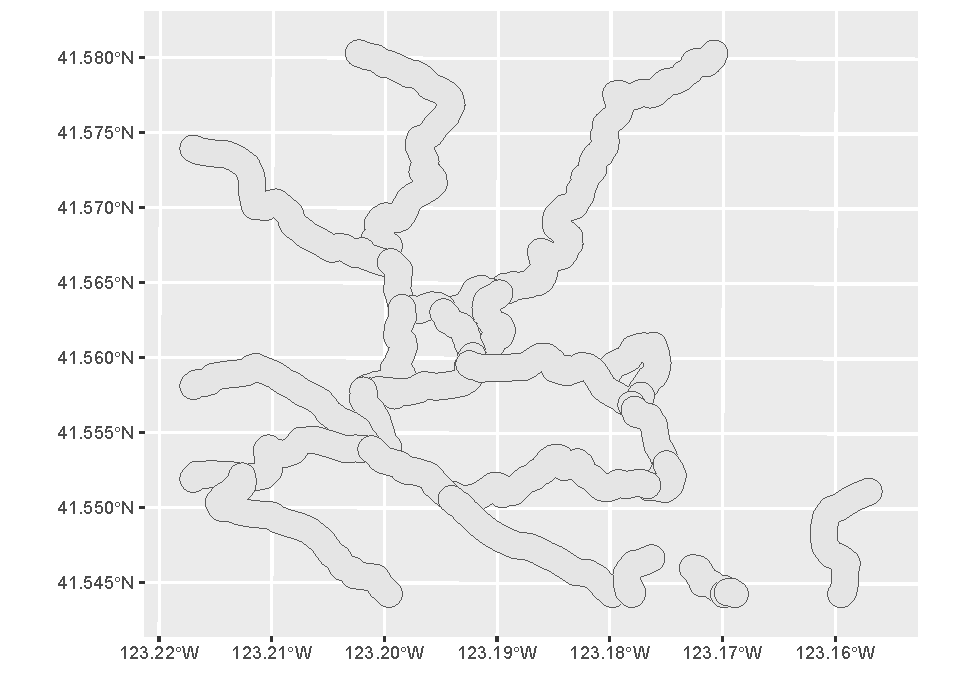
\includegraphics[width=0.75\linewidth]{EnvDataScience_files/figure-latex/spanlTrailBuffer-1} 

}

\caption{100 m trail buffer, Marble Mountains}\label{fig:spanlTrailBuffer}
\end{figure}

\begin{Shaded}
\begin{Highlighting}[]
\FunctionTok{library}\NormalTok{(igisci); }\FunctionTok{library}\NormalTok{(terra); }\FunctionTok{library}\NormalTok{(tmap)}
\NormalTok{trailsV }\OtherTok{\textless{}{-}} \FunctionTok{vect}\NormalTok{(}\FunctionTok{ex}\NormalTok{(}\StringTok{"marbles/trails.shp"}\NormalTok{))}
\NormalTok{trail\_bufft }\OtherTok{=} \FunctionTok{aggregate}\NormalTok{(}\FunctionTok{buffer}\NormalTok{(trailsV,}\DecValTok{100}\NormalTok{))}
\FunctionTok{tm\_graticules}\NormalTok{(}\AttributeTok{alpha=}\FloatTok{0.5}\NormalTok{) }\SpecialCharTok{+} \FunctionTok{tm\_shape}\NormalTok{(trail\_bufft) }\SpecialCharTok{+} \FunctionTok{tm\_polygons}\NormalTok{()}
\end{Highlighting}
\end{Shaded}

\begin{center}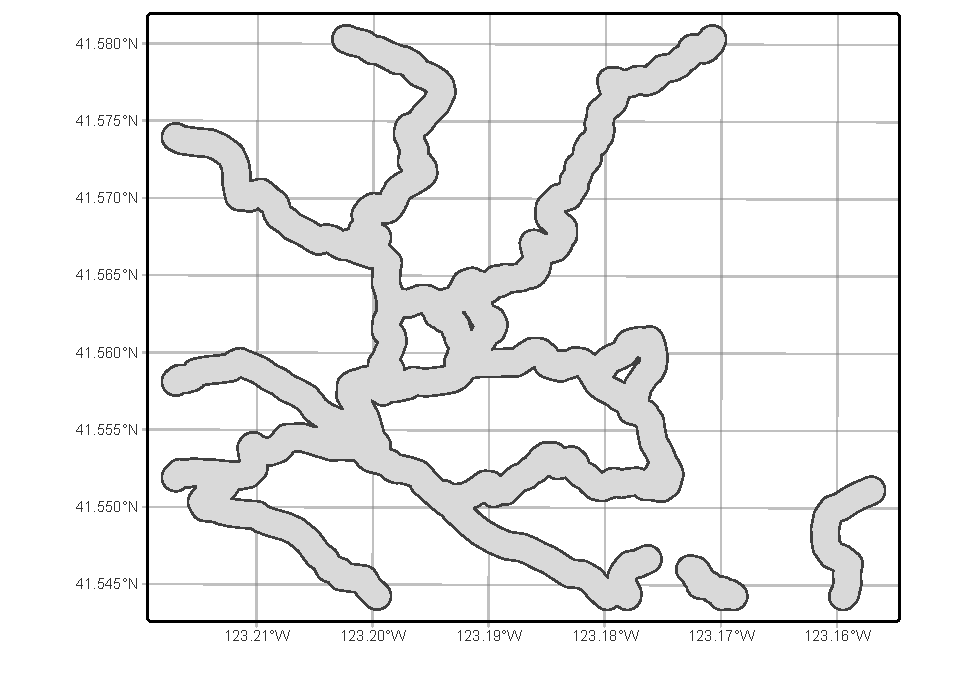
\includegraphics[width=0.75\linewidth]{EnvDataScience_files/figure-latex/spanlTrailBuffer_terra-1} \end{center}

\subsubsection{\texorpdfstring{The \texttt{units} package}{The units package}}\label{the-units-package}

\index{units}Since the spatial data is in UTM, we can just specify the distance in metres. However if the data was in decimal degrees of latitude and longitude (GCS), we would need to let the function know that we're providing it metres so it can transform that to work with the GCS, using \texttt{units::set\_units(100,\ "m")} instead of just \texttt{100}, for the above example where we are creating a 100 m buffer.

\subsection{Spatial overlay: union and intersection}\label{spatial-overlay-union-and-intersection}

\index{overlay}Overlay operations are described in the \texttt{sf} cheat sheet under ``Geometry operations''. These are useful to explore, but a couple we'll look at are union and intersection.

Normally these methods have multiple inputs, but we'll start with one that can also be used to dissolve boundaries, \index{st\_union}\textbf{\texttt{st\_union}} -- if only one input is provided it appears to do a dissolve (Figure \ref{fig:spanlUnionBuffer}):

\begin{Shaded}
\begin{Highlighting}[]
\NormalTok{trail\_buff }\OtherTok{\textless{}{-}} \FunctionTok{st\_union}\NormalTok{(trail\_buff0)}
\FunctionTok{ggplot}\NormalTok{(trail\_buff) }\SpecialCharTok{+} \FunctionTok{geom\_sf}\NormalTok{()}
\end{Highlighting}
\end{Shaded}

\begin{figure}

{\centering 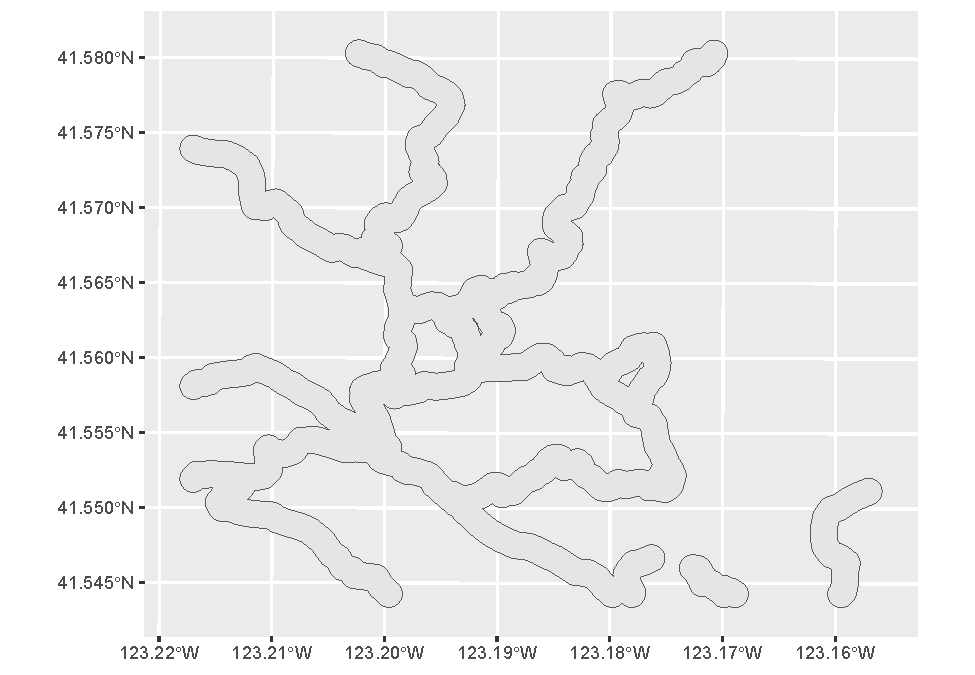
\includegraphics[width=0.75\linewidth]{EnvDataScience_files/figure-latex/spanlUnionBuffer-1} 

}

\caption{Unioned trail buffer, dissolving boundaries}\label{fig:spanlUnionBuffer}
\end{figure}

For a clearer example with the normal multiple input, we'll \index{intersect}\textbf{intersect} a 100 m buffer around streams and a 100 m buffer around trails \index{st\_intersect}\ldots{}

\begin{Shaded}
\begin{Highlighting}[]
\NormalTok{streams }\OtherTok{\textless{}{-}} \FunctionTok{st\_read}\NormalTok{(}\FunctionTok{ex}\NormalTok{(}\StringTok{"marbles/streams.shp"}\NormalTok{))}
\NormalTok{trail\_buff }\OtherTok{\textless{}{-}} \FunctionTok{st\_buffer}\NormalTok{(trails, }\DecValTok{100}\NormalTok{)}
\NormalTok{str\_buff }\OtherTok{\textless{}{-}} \FunctionTok{st\_buffer}\NormalTok{(streams,}\DecValTok{100}\NormalTok{)}
\NormalTok{strtrInt }\OtherTok{\textless{}{-}} \FunctionTok{st\_intersection}\NormalTok{(trail\_buff,str\_buff)}
\end{Highlighting}
\end{Shaded}

\ldots to show areas that are close to streams and trails (Figure \ref{fig:spanlIntTrailStrBuff}):

\begin{Shaded}
\begin{Highlighting}[]
\FunctionTok{ggplot}\NormalTok{(strtrInt) }\SpecialCharTok{+} \FunctionTok{geom\_sf}\NormalTok{(}\AttributeTok{fill=}\StringTok{"green"}\NormalTok{) }\SpecialCharTok{+} 
  \FunctionTok{geom\_sf}\NormalTok{(}\AttributeTok{data=}\NormalTok{trails, }\AttributeTok{col=}\StringTok{"red"}\NormalTok{) }\SpecialCharTok{+}
  \FunctionTok{geom\_sf}\NormalTok{(}\AttributeTok{data=}\NormalTok{streams, }\AttributeTok{col=}\StringTok{"blue"}\NormalTok{)}
\end{Highlighting}
\end{Shaded}

\begin{figure}

{\centering 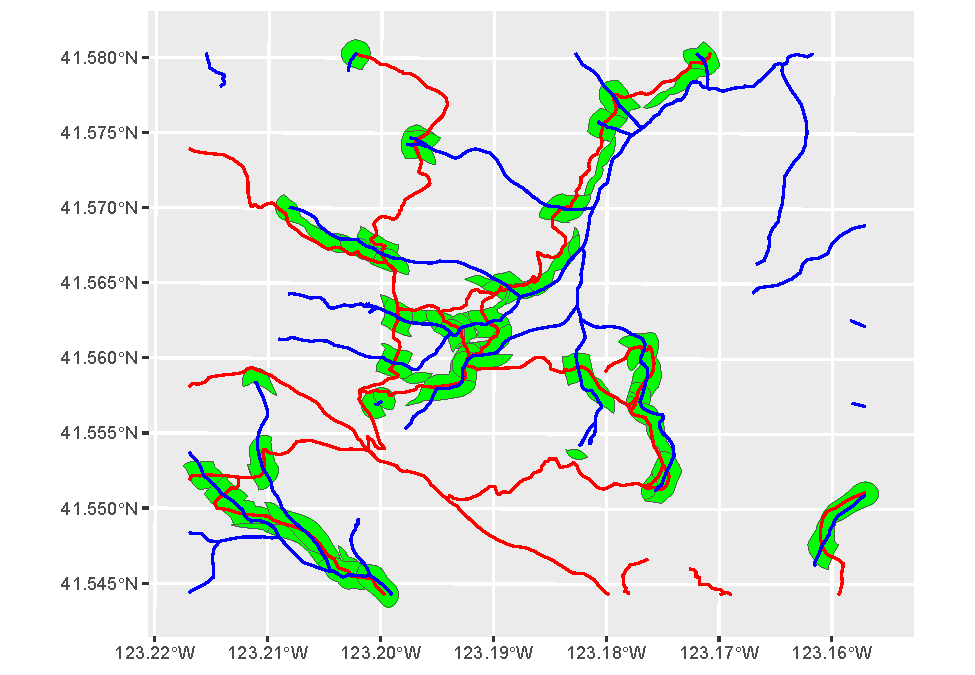
\includegraphics[width=0.75\linewidth]{EnvDataScience_files/figure-latex/spanlIntTrailStrBuff-1} 

}

\caption{Intersection of trail and stream buffers}\label{fig:spanlIntTrailStrBuff}
\end{figure}

Or how about a union of these two buffers? We'll also dissolve the boundaries using union with a single input (the first union) to dissolve those internal overlays (Figure \ref{fig:spanlUnion2buffs}):

\begin{Shaded}
\begin{Highlighting}[]
\NormalTok{strtrUnion }\OtherTok{\textless{}{-}} \FunctionTok{st\_union}\NormalTok{(}\FunctionTok{st\_union}\NormalTok{(trail\_buff,str\_buff))}
\FunctionTok{ggplot}\NormalTok{(strtrUnion) }\SpecialCharTok{+} \FunctionTok{geom\_sf}\NormalTok{(}\AttributeTok{fill=}\StringTok{"green"}\NormalTok{) }\SpecialCharTok{+} 
  \FunctionTok{geom\_sf}\NormalTok{(}\AttributeTok{data=}\NormalTok{trails, }\AttributeTok{col=}\StringTok{"red"}\NormalTok{) }\SpecialCharTok{+}
  \FunctionTok{geom\_sf}\NormalTok{(}\AttributeTok{data=}\NormalTok{streams, }\AttributeTok{col=}\StringTok{"blue"}\NormalTok{)}
\end{Highlighting}
\end{Shaded}

\begin{figure}

{\centering 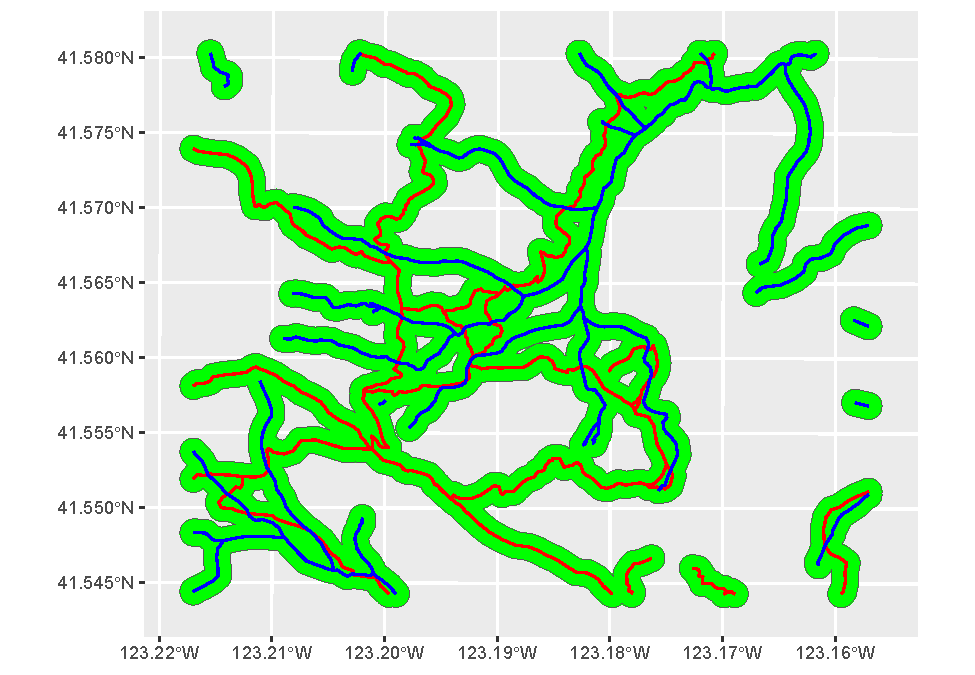
\includegraphics[width=0.75\linewidth]{EnvDataScience_files/figure-latex/spanlUnion2buffs-1} 

}

\caption{Union of two sets of buffer polygons}\label{fig:spanlUnion2buffs}
\end{figure}

\begin{quote}
Note that it is common to need to use \texttt{st\_make\_valid()} to fix slivers in buffers, though this isn't necessary here, and may occur more frequently with coarser scale data.
\end{quote}

\subsection{Clip with st\_crop}\label{clip-with-st_crop}

\index{clip}\index{st\_crop}Clipping a GIS layer to a rectangle (or to a polygon) is often useful. We'll clip to a rectangle based on latitude and longitude limits we'll specify, however since our data is in UTM, we'll need to use \textbf{\texttt{st\_transform}} to get it to the right coordinates (Figure \ref{fig:spanlCrop}).

\begin{Shaded}
\begin{Highlighting}[]
\NormalTok{xmin}\OtherTok{=}\SpecialCharTok{{-}}\FloatTok{123.21}\NormalTok{; xmax}\OtherTok{=}\SpecialCharTok{{-}}\FloatTok{123.18}\NormalTok{; ymin}\OtherTok{=}\FloatTok{41.55}\NormalTok{; ymax}\OtherTok{=}\FloatTok{41.57}
\NormalTok{clipMatrix }\OtherTok{\textless{}{-}} \FunctionTok{rbind}\NormalTok{(}\FunctionTok{c}\NormalTok{(xmin,ymin),}\FunctionTok{c}\NormalTok{(xmin,ymax),}\FunctionTok{c}\NormalTok{(xmax,ymax),}
                    \FunctionTok{c}\NormalTok{(xmax,ymin),}\FunctionTok{c}\NormalTok{(xmin,ymin))}
\NormalTok{clipGCS }\OtherTok{\textless{}{-}} \FunctionTok{st\_sfc}\NormalTok{(}\FunctionTok{st\_polygon}\NormalTok{(}\FunctionTok{list}\NormalTok{(clipMatrix)),}\AttributeTok{crs=}\DecValTok{4326}\NormalTok{)}
\NormalTok{bufferCrop }\OtherTok{\textless{}{-}} \FunctionTok{st\_crop}\NormalTok{(strtrUnion,}\FunctionTok{st\_transform}\NormalTok{(clipGCS,}\AttributeTok{crs=}\FunctionTok{st\_crs}\NormalTok{(strtrUnion)))}
\NormalTok{bnd }\OtherTok{\textless{}{-}} \FunctionTok{st\_bbox}\NormalTok{(bufferCrop)}
\FunctionTok{ggplot}\NormalTok{(bufferCrop) }\SpecialCharTok{+} \FunctionTok{geom\_sf}\NormalTok{(}\AttributeTok{fill=}\StringTok{"green"}\NormalTok{) }\SpecialCharTok{+} 
  \FunctionTok{geom\_sf}\NormalTok{(}\AttributeTok{data=}\NormalTok{trails, }\AttributeTok{col=}\StringTok{"red"}\NormalTok{) }\SpecialCharTok{+}
  \FunctionTok{geom\_sf}\NormalTok{(}\AttributeTok{data=}\NormalTok{streams, }\AttributeTok{col=}\StringTok{"blue"}\NormalTok{) }\SpecialCharTok{+}
  \FunctionTok{coord\_sf}\NormalTok{(}\AttributeTok{xlim =} \FunctionTok{c}\NormalTok{(bnd[}\DecValTok{1}\NormalTok{], bnd[}\DecValTok{3}\NormalTok{]), }\AttributeTok{ylim =} \FunctionTok{c}\NormalTok{(bnd[}\DecValTok{2}\NormalTok{], bnd[}\DecValTok{4}\NormalTok{]))}
\end{Highlighting}
\end{Shaded}

\begin{figure}

{\centering 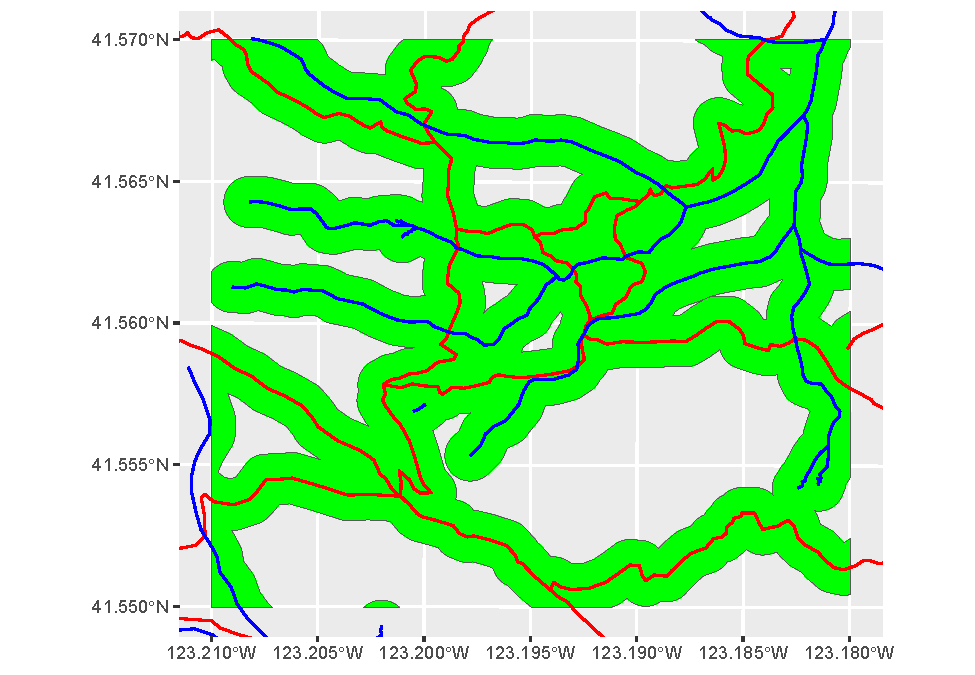
\includegraphics[width=0.75\linewidth]{EnvDataScience_files/figure-latex/spanlCrop-1} 

}

\caption{Cropping with specified x and y limits}\label{fig:spanlCrop}
\end{figure}

\subsubsection{sf or terra for vector spatial operations?}\label{sf-or-terra-for-vector-spatial-operations}

Note: there are other geometric operations in \texttt{sf} beyond what we've looked at. See the cheat sheet and other resources at \url{https://r-spatial.github.io/sf} .

The \texttt{terra} system also has many vector tools (such as \texttt{terra::union} and \texttt{terra::buffer}), that work with and create SpatVector spatial data objects. As noted earlier, these S4 spatial data can be created from (S3) sf data with \texttt{terra::vect} and vice versa with \texttt{sf::st\_as\_sf}. We'll mostly focus on sf for vector and terra for raster, but to learn more about SpatVector data and operations in terra, see \url{https://rspatial.org}.

For instance, there's a similar \texttt{terra} operation for one of the things we just did, but instead of using \texttt{union} to dissolve the internal boundaries like \texttt{st\_union} did, uses \index{aggregate}\texttt{aggregate} to remove boundaries between polygons with the same codes:

\begin{Shaded}
\begin{Highlighting}[]
\NormalTok{trails }\OtherTok{\textless{}{-}} \FunctionTok{vect}\NormalTok{(}\FunctionTok{ex}\NormalTok{(}\StringTok{"marbles/trails.shp"}\NormalTok{))}
\NormalTok{trailbuff }\OtherTok{\textless{}{-}} \FunctionTok{aggregate}\NormalTok{(}\FunctionTok{buffer}\NormalTok{(trails,}\DecValTok{100}\NormalTok{))}
\FunctionTok{plot}\NormalTok{(trailbuff)}
\end{Highlighting}
\end{Shaded}

\subsection{\texorpdfstring{Spatial join with \texttt{st\_join}}{Spatial join with st\_join}}\label{spatial-join-with-st_join}

\index{st\_join}A spatial join can do many things, but we'll just look at its simplest application -- connecting a point with the polygon that it's in. In this case, we want to join the attribute data in \texttt{BayAreaTracts} with EPA Toxic Release Inventory (TRI) point data (at factories and other point sources) and then display a few ethnicity variables from the census, associated spatially with the TRI point locations. We'll be making better maps later; this is a quick \texttt{plot()} display to show that the spatial join worked (Figure \ref{fig:spanlTRIspatialJoin}).

\begin{Shaded}
\begin{Highlighting}[]
\FunctionTok{library}\NormalTok{(igisci); }\FunctionTok{library}\NormalTok{(tidyverse); }\FunctionTok{library}\NormalTok{(sf)}
\NormalTok{TRI\_sp }\OtherTok{\textless{}{-}} \FunctionTok{st\_as\_sf}\NormalTok{(}\FunctionTok{read\_csv}\NormalTok{(}\FunctionTok{ex}\NormalTok{(}\StringTok{"TRI/TRI\_2017\_CA.csv"}\NormalTok{)), }
                   \AttributeTok{coords =} \FunctionTok{c}\NormalTok{(}\StringTok{"LONGITUDE"}\NormalTok{, }\StringTok{"LATITUDE"}\NormalTok{), }\AttributeTok{crs=}\DecValTok{4326}\NormalTok{) }\SpecialCharTok{\%\textgreater{}\%}
  \FunctionTok{st\_join}\NormalTok{(}\FunctionTok{st\_make\_valid}\NormalTok{(BayAreaTracts)) }\SpecialCharTok{\%\textgreater{}\%}
  \FunctionTok{filter}\NormalTok{(}\SpecialCharTok{!}\FunctionTok{is.na}\NormalTok{(TRACT)) }\SpecialCharTok{\%\textgreater{}\%}  \CommentTok{\# removes points not in BayAreaTracts}
\NormalTok{  dplyr}\SpecialCharTok{::}\FunctionTok{select}\NormalTok{(POP2012}\SpecialCharTok{:}\NormalTok{HISPANIC)}
\FunctionTok{plot}\NormalTok{(TRI\_sp)}
\end{Highlighting}
\end{Shaded}

\begin{figure}

{\centering 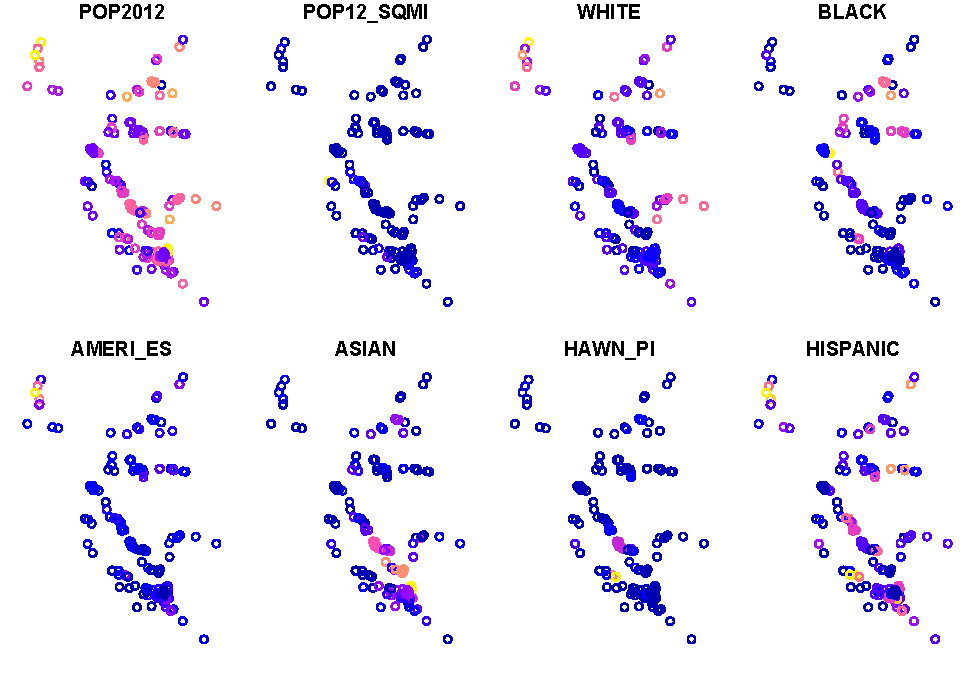
\includegraphics[width=0.75\linewidth]{EnvDataScience_files/figure-latex/spanlTRIspatialJoin-1} 

}

\caption{TRI points with census variables added via a spatial join}\label{fig:spanlTRIspatialJoin}
\end{figure}

\subsection{Further exploration of spatial analysis}\label{further-exploration-of-spatial-analysis}

We've looked at a small selection of spatial analysis functions; there's a lot more we can do, and the R spatial world is rapidly growing. There are many other methods discussed in the ``Spatial data operations'' and ``Geometry operations'' chapters of \emph{Geocomputation} (\url{https://geocompr.robinlovelace.net/}, Lovelace et al. (\citeproc{ref-Geocomputation}{2019})) that are worth exploring, and still others in the \texttt{terra} package described at \url{https://rspatial.org}, Hijmans (\citeproc{ref-rspatial}{n.d.}).

For example, getting a good handle on coordinate systems is certainly an important area to learn more about, and you will find coverage of transformation and reprojection methods in the ``Reprojecting geographic data'' and data access methods in the ``Geographic data I/O'' chapter of \emph{Geocomputation}, and in the ``Coordinate Reference Systems'' section of \url{https://rspatial.org}. The Simple Features for R reference (\emph{Simple Features for r} (\citeproc{ref-sf}{n.d.})) site includes a complete reference for all of its functions, as does \url{https://rspatial.org} for \texttt{terra}.

And then there's analysis of raster data, but we'll leave that for the next chapter.

\pagebreak

\section{Exercises: Spatial Analysis}\label{exercises-spatial-analysis}

\begin{exercise}
\textbf{Maximum Elevation} Assuming you wrote them in the last chapter (exercise questions 5 and 6), read in your western states and peaks data (pay attention to what folder they are stored in), then use a spatial join to add the peak points to the states to provide a new attribute maximum elevation, and use methods from 6.6 to display those as point labels. Note that joining from the states to the peaks works because there's a one-to-one correspondence between states and maximum peaks. (If you didn't write them, you'll need to repeat your code that built them from the previous chapter.)
\end{exercise}

\begin{center}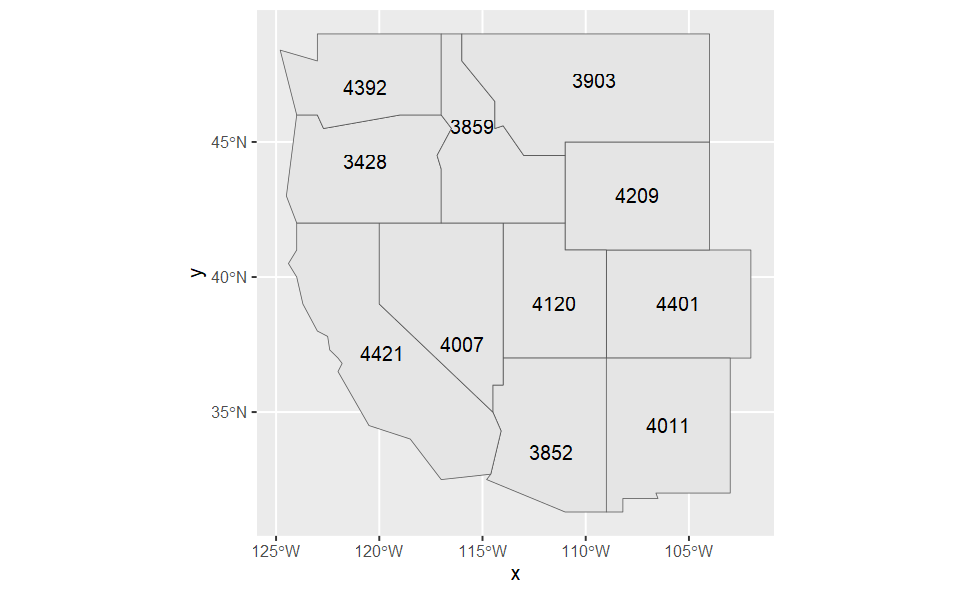
\includegraphics[width=0.6\linewidth]{img/spanl_ex1} \end{center}

\begin{exercise}
Using two shape files of your own choice, not from \texttt{igisci}, read them in as simple features data, and perform a spatial join to join the polygons to the point data. Then display the point feature data frame, and using methods from 4.4, create a scatter plot or boxplot graph (depending on the nature of your variables) where the two variables are related, preferably with a separate factor to provide color. {[}If you do not have available shapefiles, you can use \texttt{co2july95.shp} and \texttt{geology.shp} from the \texttt{marbles} folder in \texttt{extdata}, but first copy these to your project folder; one point of this is to not solely depend on \texttt{igisci} and be comfortable bringing in your own data.{]}
\end{exercise}

\begin{center}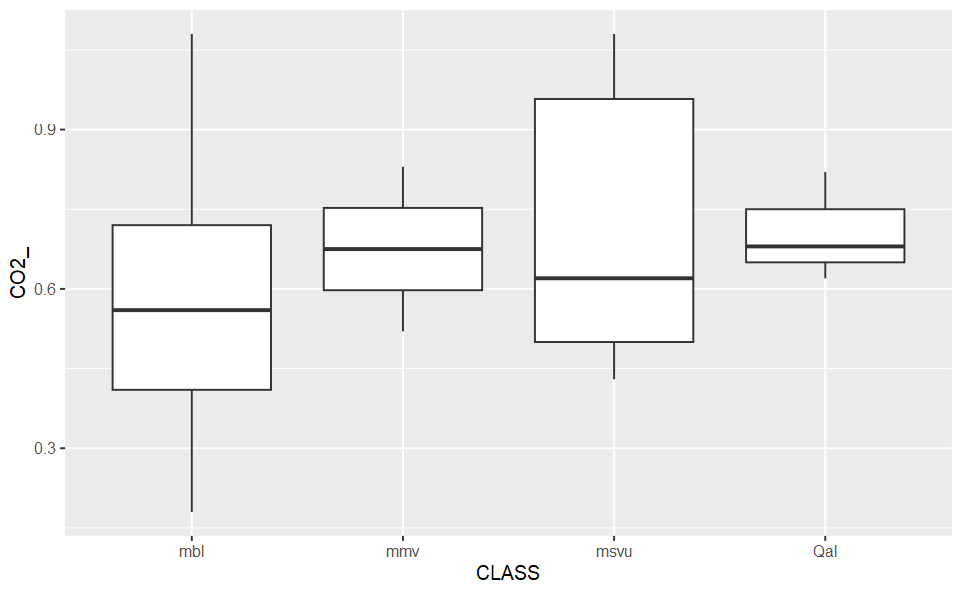
\includegraphics[width=0.75\linewidth]{img/spanl_ex2} \end{center}

\begin{exercise}
From the above spatially joined data create a map where the points are colored by data brought in from the spatial join; can be either a categorical or continuous variable.
\end{exercise}

\begin{center}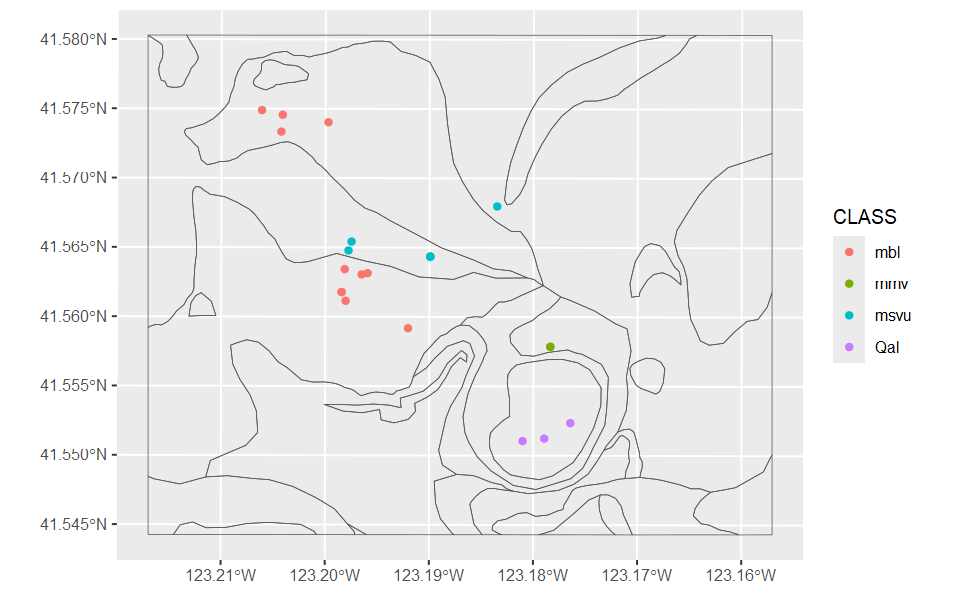
\includegraphics[width=0.75\linewidth]{img/spanl_ex3} \end{center}

\begin{exercise}
\textbf{Transect Buffers}: Using data described in 10.5.3.1, create a map using cartographic methods 6.8 of transects, the mainland (for context, similar to a basemap), and a 1000 m buffer around the transect points, using methods from 7.2.4 and 7.2.5. Note that mainland.shp is in the SFmarine folder of the igisci extdata.
\end{exercise}

\begin{center}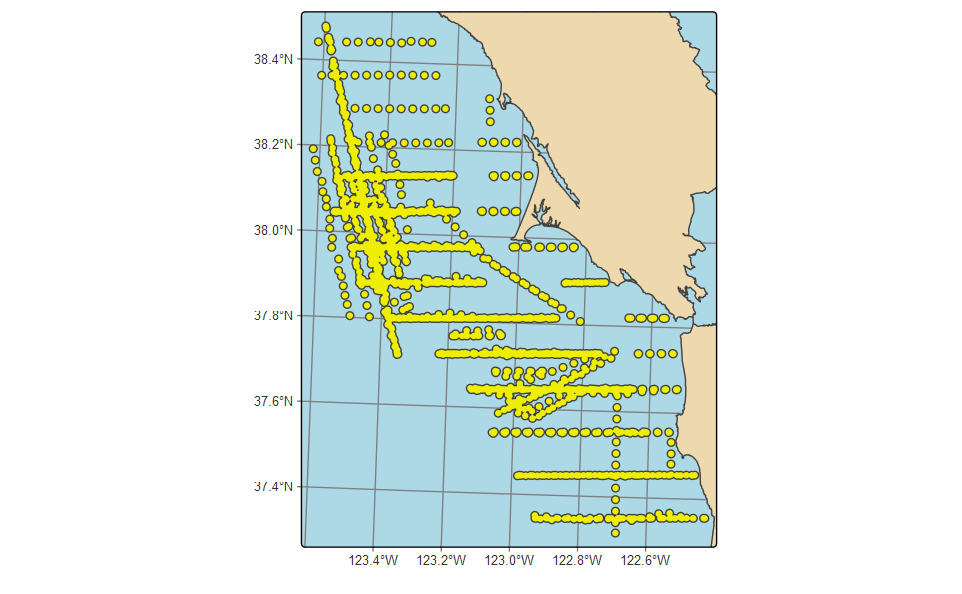
\includegraphics[width=0.75\linewidth]{img/spanl_ex4} \end{center}

\begin{exercise}

Create an sf that represents all areas within 50 km (see 7.2.4) of a TRI facility in California that has \textgreater10,000 pounds of total stack air release for all gases, clipped (intersected) with the state of California as provided in the CA counties data set. Then use this to create a map of California showing the clipped buffered areas in red, with California counties and those selected large-release TRI facilities in black dots, as shown here. For the buffer distances, make sure to use the function described in 7.2.4.1 to get the units right despite the map being in GCS. Methods from 3.4.5 will be useful, and you'll need to use \texttt{st\_make\_valid} with buffer results to avoid errors.

\begin{center}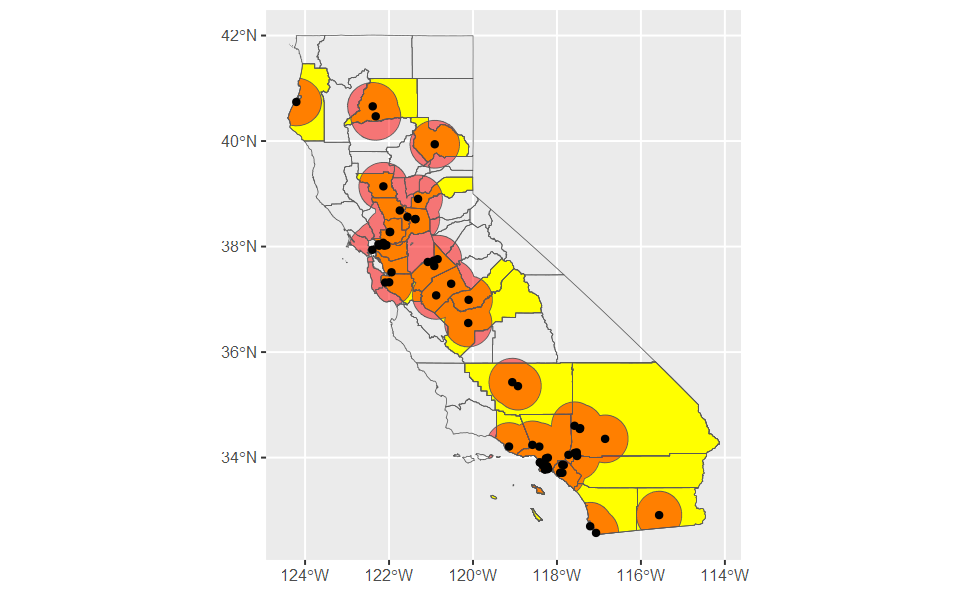
\includegraphics[width=0.75\linewidth]{img/spanl_ex5} \end{center}

\end{exercise}

\chapter{Raster Spatial Analysis}\label{raster}

\index{raster spatial analysis}Raster spatial analysis is particularly important in environmental analysis, since much environmental data is continuous in nature, based on continuous measurements \index{continuous measurements}from instruments (like temperature, pH, air pressure, water depth, elevation), and raster models work well with continuous data. In the Spatial Data and Maps chapter, we looked at creating rasters from scratch, or converted from features, and visualizing them. Here we'll explore raster analytical methods, commonly working from existing information-rich rasters like elevation data, where we'll start by looking at terrain functions.

We'll make a lot of use of \texttt{terra} functions in this chapter\index{terra}, as this package is replacing the \texttt{raster} package which has been widely used. One raster package that's probably also worth considering is the \texttt{stars} package.

\section{Terrain functions}\label{terrain}

\index{terrain functions}Elevation data is particularly information-rich, and a lot can be derived from them that informs us about the nature of landscapes and what drives surface hydrologic and geomorphic processes as well as biotic habitat (some slopes are drier than others, for instance). We'll start by reading in some elevation data from the Marble Mountains of California (Figure \ref{fig:rasMblElev}) and use terra's terrain function to derive slope\index{slope} (Figure \ref{fig:rasSlope}), aspect\index{aspect} (Figure \ref{fig:rasAspect}), and hillshade\index{hillshade} rasters.

\begin{Shaded}
\begin{Highlighting}[]
\FunctionTok{library}\NormalTok{(terra); }\FunctionTok{library}\NormalTok{(igisci)}
\NormalTok{elev }\OtherTok{\textless{}{-}} \FunctionTok{rast}\NormalTok{(}\FunctionTok{ex}\NormalTok{(}\StringTok{"marbles/elev.tif"}\NormalTok{))}
\FunctionTok{plot}\NormalTok{(elev)}
\end{Highlighting}
\end{Shaded}

\begin{figure}

{\centering 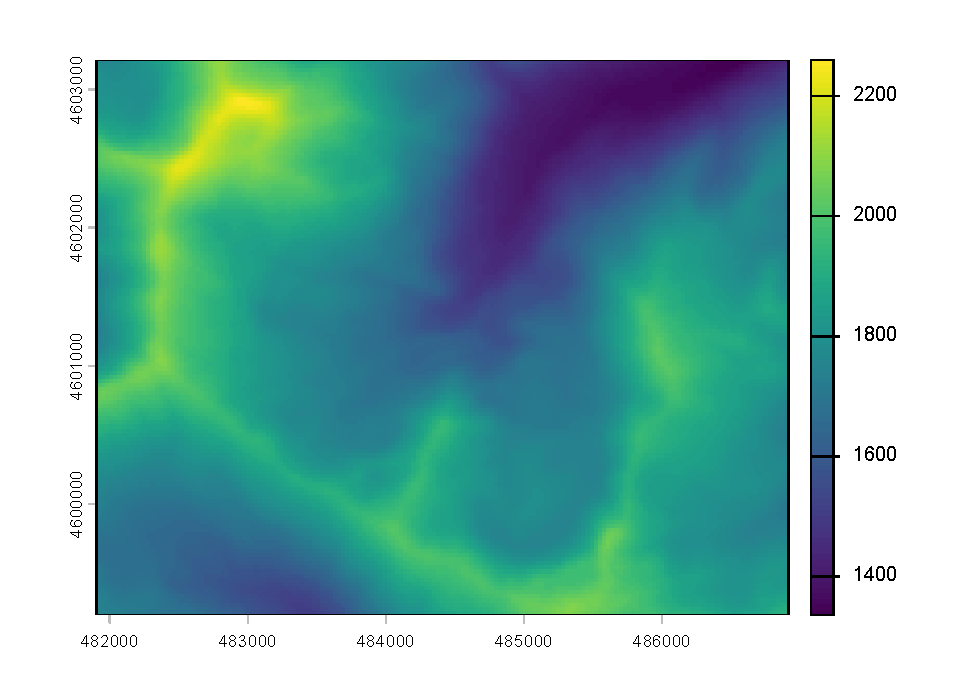
\includegraphics[width=0.75\linewidth]{EnvDataScience_files/figure-latex/rasMblElev-1} 

}

\caption{Marble Mountains (California) elevation}\label{fig:rasMblElev}
\end{figure}

\begin{Shaded}
\begin{Highlighting}[]
\NormalTok{slope }\OtherTok{\textless{}{-}} \FunctionTok{terrain}\NormalTok{(elev, }\AttributeTok{v=}\StringTok{"slope"}\NormalTok{)}
\FunctionTok{plot}\NormalTok{(slope)}
\end{Highlighting}
\end{Shaded}

\begin{figure}

{\centering 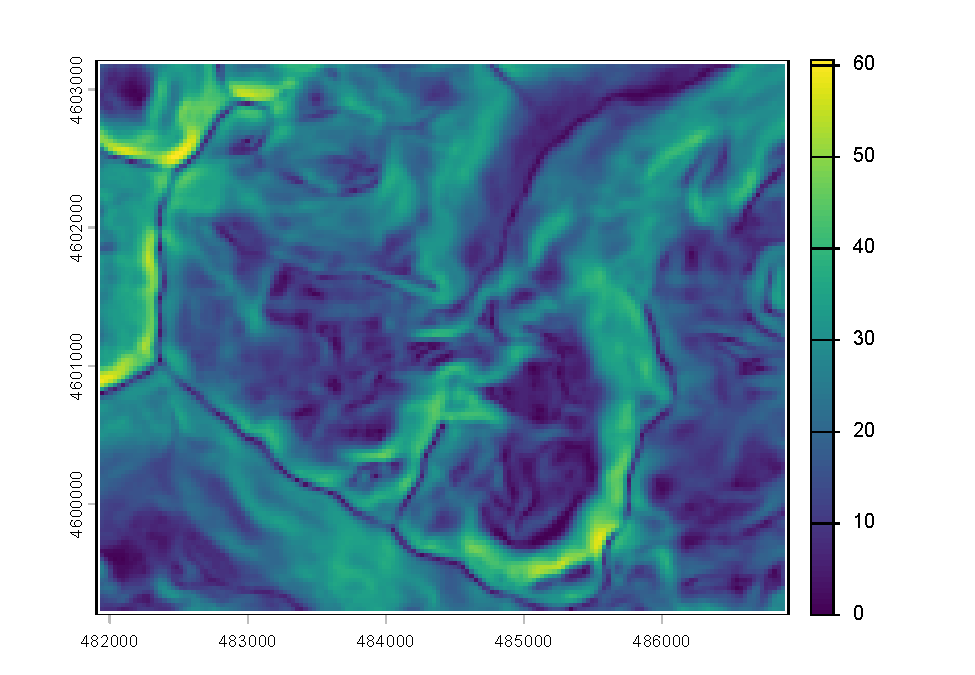
\includegraphics[width=0.75\linewidth]{EnvDataScience_files/figure-latex/rasSlope-1} 

}

\caption{Slope}\label{fig:rasSlope}
\end{figure}

\begin{Shaded}
\begin{Highlighting}[]
\NormalTok{aspect }\OtherTok{\textless{}{-}} \FunctionTok{terrain}\NormalTok{(elev, }\AttributeTok{v=}\StringTok{"aspect"}\NormalTok{)}
\FunctionTok{plot}\NormalTok{(aspect)}
\end{Highlighting}
\end{Shaded}

\begin{figure}

{\centering 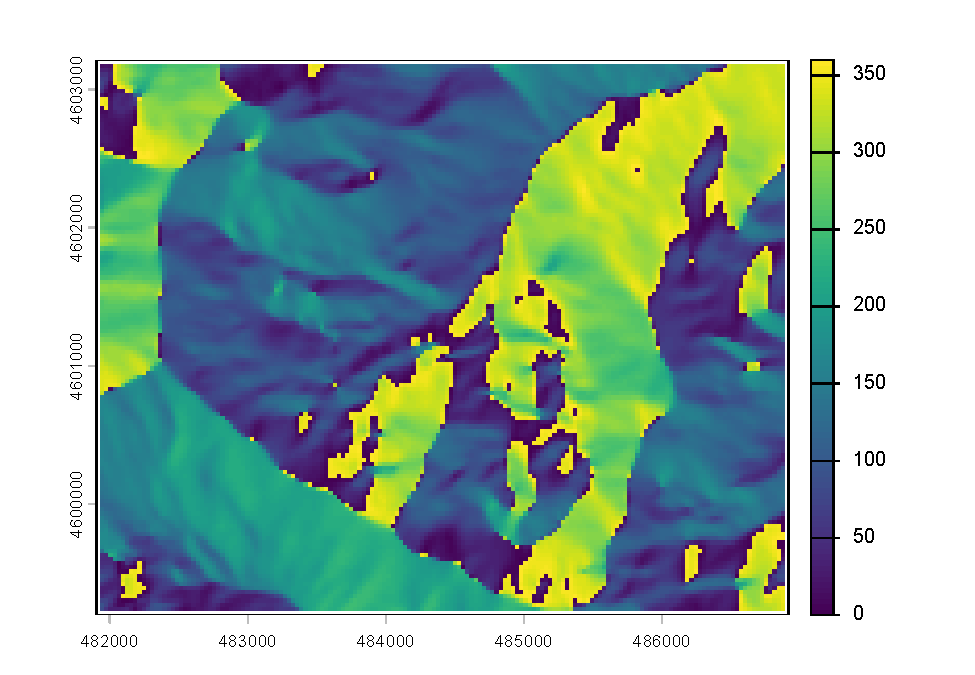
\includegraphics[width=0.75\linewidth]{EnvDataScience_files/figure-latex/rasAspect-1} 

}

\caption{Aspect}\label{fig:rasAspect}
\end{figure}

\ldots{} then we'll use \index{classify, terra}terra::classify to make six discrete categorical slope classes (though the legend suggests it's continuous) (Figure \ref{fig:rasClassifiedSlope})\ldots{}

\begin{Shaded}
\begin{Highlighting}[]
\NormalTok{slopeclasses }\OtherTok{\textless{}{-}}\FunctionTok{matrix}\NormalTok{(}\FunctionTok{c}\NormalTok{(}\DecValTok{00}\NormalTok{,}\DecValTok{10}\NormalTok{,}\DecValTok{1}\NormalTok{, }\DecValTok{10}\NormalTok{,}\DecValTok{20}\NormalTok{,}\DecValTok{2}\NormalTok{, }\DecValTok{20}\NormalTok{,}\DecValTok{30}\NormalTok{,}\DecValTok{3}\NormalTok{,}
                        \DecValTok{30}\NormalTok{,}\DecValTok{40}\NormalTok{,}\DecValTok{4}\NormalTok{, }\DecValTok{40}\NormalTok{,}\DecValTok{50}\NormalTok{,}\DecValTok{5}\NormalTok{, }\DecValTok{50}\NormalTok{,}\DecValTok{90}\NormalTok{,}\DecValTok{6}\NormalTok{), }\AttributeTok{ncol=}\DecValTok{3}\NormalTok{, }\AttributeTok{byrow=}\ConstantTok{TRUE}\NormalTok{)}
\NormalTok{slopeclass }\OtherTok{\textless{}{-}} \FunctionTok{classify}\NormalTok{(slope, }\AttributeTok{rcl =}\NormalTok{ slopeclasses)}
\FunctionTok{plot}\NormalTok{(slopeclass)}
\end{Highlighting}
\end{Shaded}

\begin{figure}

{\centering 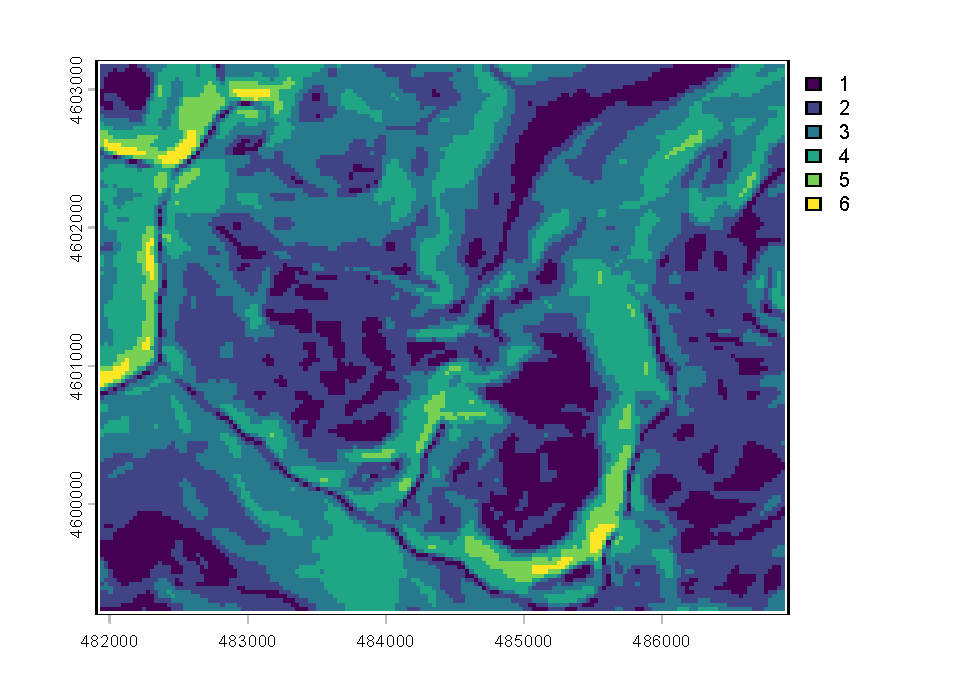
\includegraphics[width=0.75\linewidth]{EnvDataScience_files/figure-latex/rasClassifiedSlope-1} 

}

\caption{Classified slopes}\label{fig:rasClassifiedSlope}
\end{figure}

Then a \index{shade, terra}hillshade effect raster with slope and aspect as inputs after converting to radians (Figure \ref{fig:rasHillshade}):

\begin{Shaded}
\begin{Highlighting}[]
\NormalTok{hillsh }\OtherTok{\textless{}{-}} \FunctionTok{shade}\NormalTok{(slope}\SpecialCharTok{/}\DecValTok{180}\SpecialCharTok{*}\NormalTok{pi, aspect}\SpecialCharTok{/}\DecValTok{180}\SpecialCharTok{*}\NormalTok{pi, }\AttributeTok{angle=}\DecValTok{40}\NormalTok{, }\AttributeTok{direction=}\DecValTok{330}\NormalTok{)}
\FunctionTok{plot}\NormalTok{(hillsh, }\AttributeTok{col=}\FunctionTok{gray}\NormalTok{(}\DecValTok{0}\SpecialCharTok{:}\DecValTok{100}\SpecialCharTok{/}\DecValTok{100}\NormalTok{))}
\end{Highlighting}
\end{Shaded}

\begin{figure}

{\centering 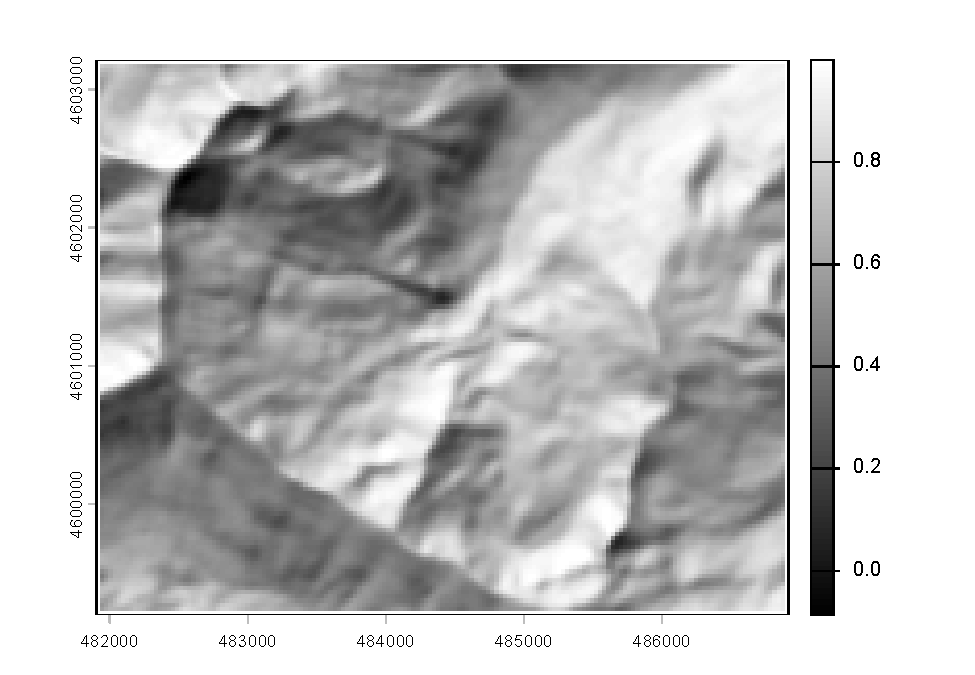
\includegraphics[width=0.75\linewidth]{EnvDataScience_files/figure-latex/rasHillshade-1} 

}

\caption{Hillshade}\label{fig:rasHillshade}
\end{figure}

\section{Map Algebra in terra}\label{map-algebra-in-terra}

\index{map algebra}Map algebra was originally developed by Dana Tomlin in the 1970s and 1980s (Tomlin (\citeproc{ref-Tomlin}{1990})), and was the basis for his Map Analysis Package. It works by assigning raster outputs from an algebraic expression of raster inputs. Map algebra was later incorporated in Esri's Grid and Spatial Analyst subsystems of ArcInfo and ArcGIS. Its simple and elegant syntax makes it still one of the best ways to manipulate raster data.

Let's look at a couple of simple map algebra statements to derive some new rasters, such as converting elevation in metres to feet (Figure \ref{fig:rasMapAlgebra}).

\begin{Shaded}
\begin{Highlighting}[]
\NormalTok{elevft }\OtherTok{\textless{}{-}}\NormalTok{ elev }\SpecialCharTok{/} \FloatTok{0.3048}
\FunctionTok{plot}\NormalTok{(elevft)}
\end{Highlighting}
\end{Shaded}

\begin{figure}

{\centering 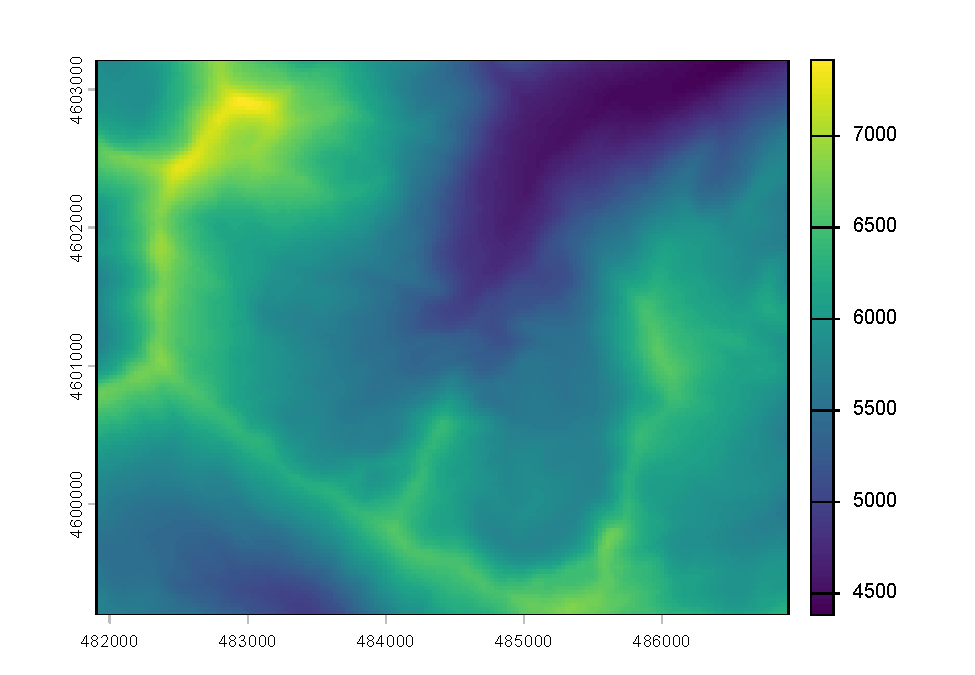
\includegraphics[width=0.75\linewidth]{EnvDataScience_files/figure-latex/rasMapAlgebra-1} 

}

\caption{Map algebra conversion of elevations from metres to feet}\label{fig:rasMapAlgebra}
\end{figure}

\ldots{} including some that create and use \index{Boolean}Boolean (true-false) values, where 1 is true and 0 is false, so might answer the question ``Is it steep?'' (as long as we understand 1 means Yes or true) (Figure \ref{fig:rasSlopeGT30})\ldots{}

\begin{Shaded}
\begin{Highlighting}[]
\NormalTok{steep }\OtherTok{\textless{}{-}}\NormalTok{ slope }\SpecialCharTok{\textgreater{}} \DecValTok{30}
\FunctionTok{plot}\NormalTok{(steep)}
\end{Highlighting}
\end{Shaded}

\begin{figure}

{\centering 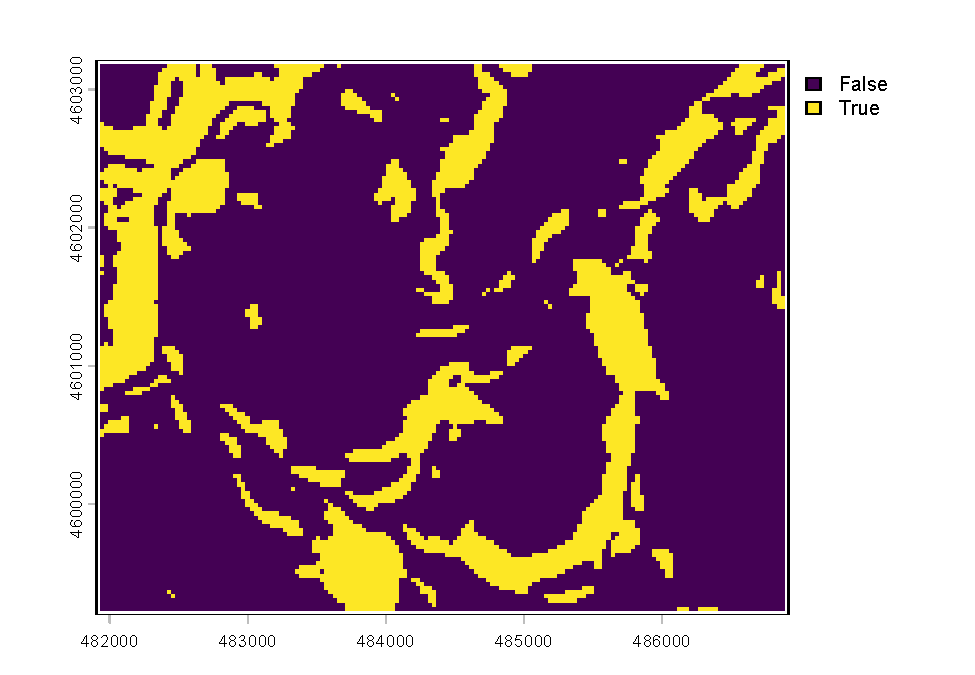
\includegraphics[width=0.75\linewidth]{EnvDataScience_files/figure-latex/rasSlopeGT30-1} 

}

\caption{Boolean: slope > 30}\label{fig:rasSlopeGT30}
\end{figure}

\ldots{} or Figure \ref{fig:rasIntersection}, which shows all areas that are steeper than 30 degrees \emph{and} above 2,000 m elevation.

\begin{Shaded}
\begin{Highlighting}[]
\FunctionTok{plot}\NormalTok{(steep }\SpecialCharTok{*}\NormalTok{ (elev }\SpecialCharTok{\textgreater{}} \DecValTok{2000}\NormalTok{))}
\end{Highlighting}
\end{Shaded}

\begin{figure}

{\centering 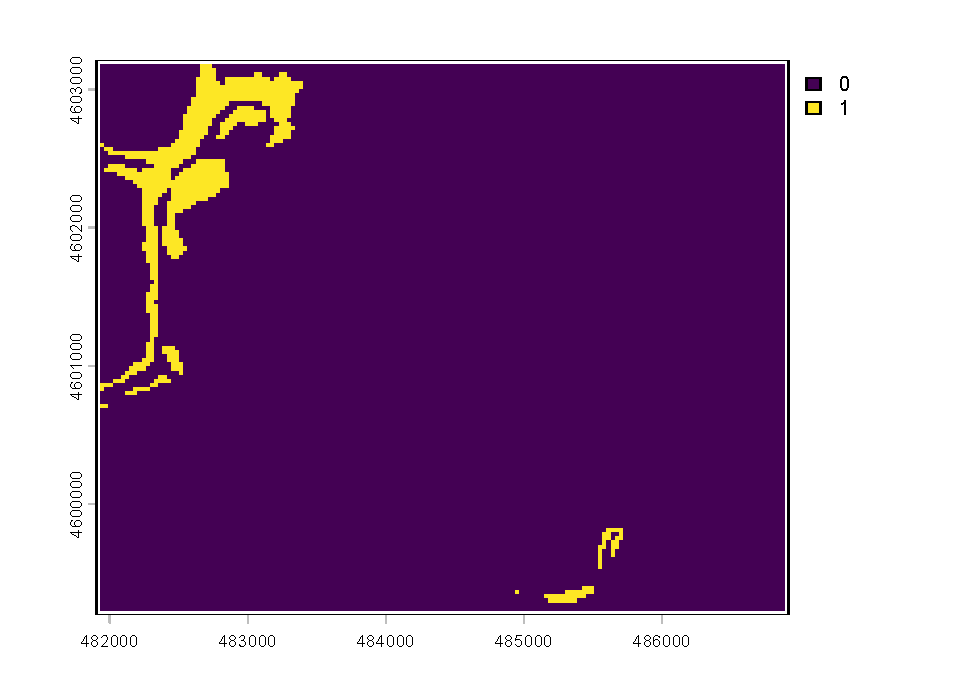
\includegraphics[width=0.75\linewidth]{EnvDataScience_files/figure-latex/rasIntersection-1} 

}

\caption{Boolean intersection: (slope > 30) * (elev > 2000)}\label{fig:rasIntersection}
\end{figure}

\begin{quote}
When plotting in tmap, it's cartographically useful to convert zeros to NA values to be transparent. I guess the same can be said for base plot or ggplot. To make the zeros transparent and plot them, try the method in the second line of code here (though it does alter the meaning of the raster \texttt{steep} with NAs instead of zeros) (Figure \ref{fig:rasSteepAreas}.
\end{quote}

Since the tm\_basemap method doesn't seem to work with rasters in tmap 4.0 (might be coming with 4.1), we could use the trick we used in the previous chapter to create a raster from the basemap and display that. We'll plot the \texttt{steep} raster before the basemap to set the bounding box properly.

\begin{Shaded}
\begin{Highlighting}[]
\FunctionTok{library}\NormalTok{(tmap); }\FunctionTok{library}\NormalTok{(maptiles); }\FunctionTok{library}\NormalTok{(sf)}
\NormalTok{steep[steep}\SpecialCharTok{==}\DecValTok{0}\NormalTok{] }\OtherTok{\textless{}{-}} \ConstantTok{NA}
\NormalTok{mblBase }\OtherTok{\textless{}{-}} \FunctionTok{get\_tiles}\NormalTok{(steep, }\AttributeTok{provider=}\StringTok{"OpenTopoMap"}\NormalTok{)}
\FunctionTok{tm\_shape}\NormalTok{(steep) }\SpecialCharTok{+} 
  \FunctionTok{tm\_raster}\NormalTok{(}\AttributeTok{col\_alpha=}\FloatTok{0.5}\NormalTok{,}
            \AttributeTok{col.scale=}\FunctionTok{tm\_scale\_categorical}\NormalTok{(}\AttributeTok{values=}\FunctionTok{c}\NormalTok{(}\StringTok{"red"}\NormalTok{)),}
            \AttributeTok{col.legend =} \FunctionTok{tm\_legend}\NormalTok{(}\StringTok{"steep"}\NormalTok{, }\AttributeTok{frame=}\NormalTok{F)) }\SpecialCharTok{+}
  \FunctionTok{tm\_shape}\NormalTok{(mblBase) }\SpecialCharTok{+} 
     \FunctionTok{tm\_rgb}\NormalTok{(}\AttributeTok{col\_alpha=}\FloatTok{0.5}\NormalTok{)}
\end{Highlighting}
\end{Shaded}

\begin{figure}

{\centering 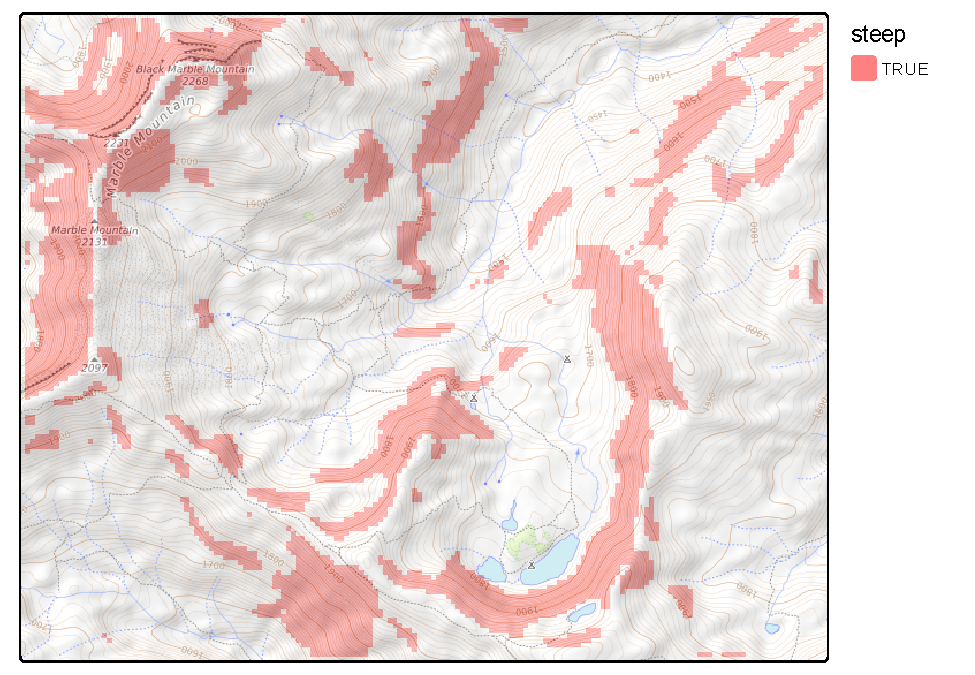
\includegraphics[width=0.75\linewidth]{EnvDataScience_files/figure-latex/rasSteepAreas-1} 

}

\caption{Steep Areas}\label{fig:rasSteepAreas}
\end{figure}

You should be able to imagine that map algebra is particularly useful when applying a \index{model equation using map algebra}model equation to data to create a prediction map. For instance, later we'll use \texttt{lm()} to derive linear regression parameters for predicting February temperature from elevation in the Sierra \ldots{}

\[
Temperature_{prediction} = 11.88 - 0.006{elevation}
\]

\ldots{} which can be coded in map algebra something like the following if we have an elevation raster, to create a tempPred raster:

\begin{Shaded}
\begin{Highlighting}[]
\NormalTok{tempPred }\OtherTok{\textless{}{-}} \FloatTok{11.88} \SpecialCharTok{{-}} \FloatTok{0.006} \SpecialCharTok{*}\NormalTok{ elev }\CommentTok{\# ation}
\end{Highlighting}
\end{Shaded}

\section{Distance}\label{distance-1}

A continuous raster of distances \index{distance, continuous raster}from significant features can be very informative in environmental analysis. For instance, distance from the coast or a body of water may be an important variable for habitat analysis and ecological niche modeling. The goal of the following is to derive distances from streams as a continuous raster.

We'll need to know what cell size to use and how far to extend our raster\index{raster structure}. If we have an existing study area raster, this process is simple. We start by converting streams from a SpatVector to a SpatRaster\index{SpatRaster}, as we did a couple of chapters ago. The \texttt{terra::distance()} function then uses this structure to provide the cells that we're deriving distance from and then uses that same cell size and extent for the output raster. If we instead used vector features, the \texttt{distance} function would return point-to-point distances, very different from deriving continuous rasters\index{continuous rasters, deriving} of Euclidean distance (Figure \ref{fig:rasStrDist}).

\begin{Shaded}
\begin{Highlighting}[]
\NormalTok{streams }\OtherTok{\textless{}{-}} \FunctionTok{vect}\NormalTok{(}\FunctionTok{ex}\NormalTok{(}\StringTok{"marbles/streams.shp"}\NormalTok{))}
\NormalTok{elev }\OtherTok{\textless{}{-}} \FunctionTok{rast}\NormalTok{(}\FunctionTok{ex}\NormalTok{(}\StringTok{"marbles/elev.tif"}\NormalTok{))}
\NormalTok{stdist }\OtherTok{\textless{}{-}}\NormalTok{ terra}\SpecialCharTok{::}\FunctionTok{distance}\NormalTok{(}\FunctionTok{rasterize}\NormalTok{(streams,elev))}
\FunctionTok{plot}\NormalTok{(stdist)}
\FunctionTok{lines}\NormalTok{(streams)}
\end{Highlighting}
\end{Shaded}

\begin{figure}

{\centering 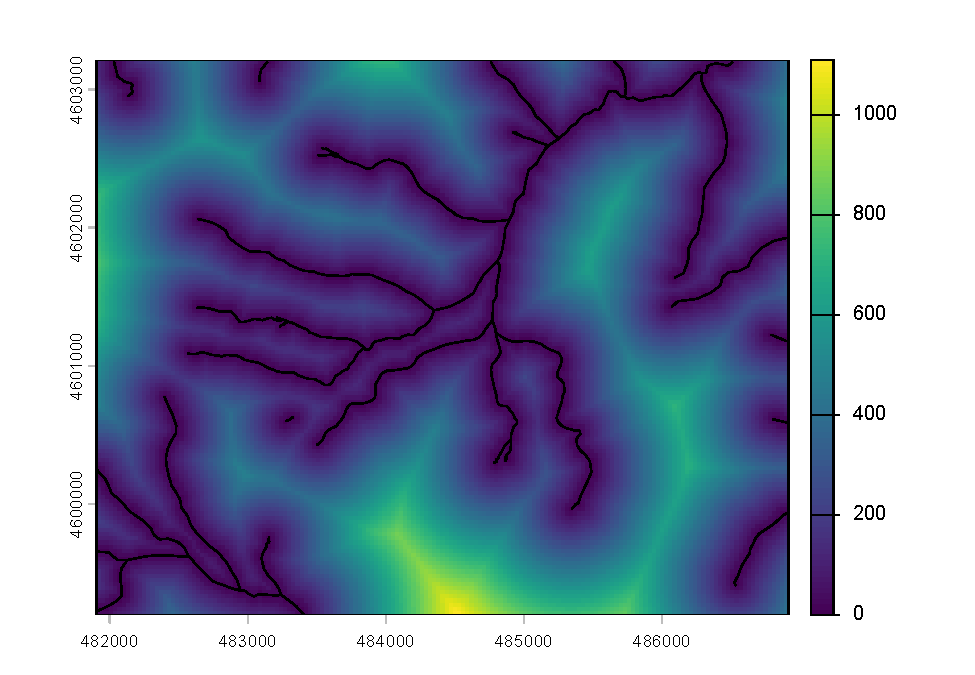
\includegraphics[width=0.75\linewidth]{EnvDataScience_files/figure-latex/rasStrDist-1} 

}

\caption{Stream distance raster}\label{fig:rasStrDist}
\end{figure}

If we didn't have an elevation raster, we could use the process we employed while converting features to rasters in the Spatial Data and Maps chapter, where we derived a raster template from the extent of streams, as shown here:

\begin{Shaded}
\begin{Highlighting}[]
\NormalTok{streams }\OtherTok{\textless{}{-}} \FunctionTok{vect}\NormalTok{(}\FunctionTok{ex}\NormalTok{(}\StringTok{"marbles/streams.shp"}\NormalTok{))}
\NormalTok{XMIN }\OtherTok{\textless{}{-}} \FunctionTok{ext}\NormalTok{(streams)}\SpecialCharTok{$}\NormalTok{xmin}
\NormalTok{XMAX }\OtherTok{\textless{}{-}} \FunctionTok{ext}\NormalTok{(streams)}\SpecialCharTok{$}\NormalTok{xmax}
\NormalTok{YMIN }\OtherTok{\textless{}{-}} \FunctionTok{ext}\NormalTok{(streams)}\SpecialCharTok{$}\NormalTok{ymin}
\NormalTok{YMAX }\OtherTok{\textless{}{-}} \FunctionTok{ext}\NormalTok{(streams)}\SpecialCharTok{$}\NormalTok{ymax}
\NormalTok{aspectRatio }\OtherTok{\textless{}{-}}\NormalTok{ (YMAX}\SpecialCharTok{{-}}\NormalTok{YMIN)}\SpecialCharTok{/}\NormalTok{(XMAX}\SpecialCharTok{{-}}\NormalTok{XMIN)}
\NormalTok{cellSize }\OtherTok{\textless{}{-}} \DecValTok{30}
\NormalTok{NCOLS }\OtherTok{\textless{}{-}} \FunctionTok{as.integer}\NormalTok{((XMAX}\SpecialCharTok{{-}}\NormalTok{XMIN)}\SpecialCharTok{/}\NormalTok{cellSize)}
\NormalTok{NROWS }\OtherTok{\textless{}{-}} \FunctionTok{as.integer}\NormalTok{(NCOLS }\SpecialCharTok{*}\NormalTok{ aspectRatio)}
\NormalTok{templateRas }\OtherTok{\textless{}{-}} \FunctionTok{rast}\NormalTok{(}\AttributeTok{ncol=}\NormalTok{NCOLS, }\AttributeTok{nrow=}\NormalTok{NROWS, }
                    \AttributeTok{xmin=}\NormalTok{XMIN, }\AttributeTok{xmax=}\NormalTok{XMAX, }\AttributeTok{ymin=}\NormalTok{YMIN, }\AttributeTok{ymax=}\NormalTok{YMAX,}
                    \AttributeTok{vals=}\DecValTok{1}\NormalTok{, }\AttributeTok{crs=}\FunctionTok{crs}\NormalTok{(streams))}
\NormalTok{strms }\OtherTok{\textless{}{-}} \FunctionTok{rasterize}\NormalTok{(streams,templateRas)}
\NormalTok{stdist }\OtherTok{\textless{}{-}}\NormalTok{ terra}\SpecialCharTok{::}\FunctionTok{distance}\NormalTok{(strms)}
\FunctionTok{plot}\NormalTok{(stdist)}
\FunctionTok{lines}\NormalTok{(streams)}
\end{Highlighting}
\end{Shaded}

\begin{quote}
In deriving distances, it's useful to remember that distances can go on forever (well, on the planet they may go around and around, if we were using spherical coordinates) so that's another reason we have to specify the raster structure we want to populate.
\end{quote}

\section{Extracting Values}\label{extracting-values}

\index{extraction from rasters}A very useful method or environmental analysis and modeling is to extract values from rasters at specific point locations. The point locations might be observations of species, soil samples, or even random points, and getting continuous (or discrete) raster observations can be very useful in a statistical analysis associated with those points. The distance from streams raster we derived earlier, or elevation, or terrain derivatives like slope and aspect might be very useful in a ecological niche model, for instance. We'll start by using random points and use these to extract values from four rasters:

\begin{itemize}
\tightlist
\item
  \textbf{elev}: read in from elev.tif
\item
  \textbf{slope}: created from elev with \textbf{terrain}
\item
  \textbf{str\_dist}: euclidean distance to streams
\item
  \textbf{geol}: rasterized\index{rasterize, terra} from geology polygon features
\end{itemize}

\begin{Shaded}
\begin{Highlighting}[]
\FunctionTok{library}\NormalTok{(igisci); }\FunctionTok{library}\NormalTok{(terra); }\FunctionTok{library}\NormalTok{(tidyverse); }\FunctionTok{library}\NormalTok{(sf)}
\NormalTok{geolshp }\OtherTok{\textless{}{-}} \FunctionTok{st\_read}\NormalTok{(}\FunctionTok{ex}\NormalTok{(}\StringTok{"marbles/geology.shp"}\NormalTok{)) }\SpecialCharTok{|\textgreater{}}
           \FunctionTok{rename}\NormalTok{(}\AttributeTok{geology=}\NormalTok{CLASS)}
\NormalTok{streams }\OtherTok{\textless{}{-}} \FunctionTok{vect}\NormalTok{(}\FunctionTok{ex}\NormalTok{(}\StringTok{"marbles/streams.shp"}\NormalTok{))}
\NormalTok{elev }\OtherTok{\textless{}{-}} \FunctionTok{rast}\NormalTok{(}\FunctionTok{ex}\NormalTok{(}\StringTok{"marbles/elev.tif"}\NormalTok{))}
\NormalTok{slope }\OtherTok{\textless{}{-}} \FunctionTok{terrain}\NormalTok{(elev, }\AttributeTok{v=}\StringTok{"slope"}\NormalTok{)}
\NormalTok{str\_dist }\OtherTok{\textless{}{-}}\NormalTok{ terra}\SpecialCharTok{::}\FunctionTok{distance}\NormalTok{(}\FunctionTok{rasterize}\NormalTok{(streams,elev))}
\NormalTok{geol }\OtherTok{\textless{}{-}} \FunctionTok{rasterize}\NormalTok{(geolshp,elev,}\AttributeTok{field=}\StringTok{"geology"}\NormalTok{) }
\end{Highlighting}
\end{Shaded}

Note that in contrast to the other rasters, the stream distance raster ends up with no name\index{names, raster}, so we should give it a name:

\begin{Shaded}
\begin{Highlighting}[]
\FunctionTok{names}\NormalTok{(slope)}
\end{Highlighting}
\end{Shaded}

\begin{verbatim}
## [1] "slope"
\end{verbatim}

\begin{Shaded}
\begin{Highlighting}[]
\FunctionTok{names}\NormalTok{(str\_dist)}
\end{Highlighting}
\end{Shaded}

\begin{verbatim}
## [1] "layer"
\end{verbatim}

\begin{Shaded}
\begin{Highlighting}[]
\FunctionTok{names}\NormalTok{(str\_dist) }\OtherTok{\textless{}{-}} \StringTok{"str\_dist"}
\end{Highlighting}
\end{Shaded}

\begin{quote}
\textbf{On the raster \texttt{names} property}: You'll find that many terra functions may not assign the \texttt{names} property you'd expect, so it's a good idea to check with \texttt{names()} and maybe set it to what we want, as we've just done for \texttt{str\_dist}. As we'll see later with the focal statistics function, the name of the input is used even though we've modified it in the function result, and that may create confusion when we use it. We just saw that the \texttt{distance()} function produced an empty name, and there may be others you'll run into. For many downstream uses, the names property may not matter, but it will be important when we extract values from rasters into points where the \texttt{names} property is assigned to the variable created for the points.
\end{quote}

Then we'll create 200 \textbf{random xy points} \ref{random} within the extent of \texttt{elev}, and assign it the same \texttt{crs}.

\begin{Shaded}
\begin{Highlighting}[]
\FunctionTok{library}\NormalTok{(sf)}
\NormalTok{x }\OtherTok{\textless{}{-}} \FunctionTok{runif}\NormalTok{(}\DecValTok{200}\NormalTok{, }\AttributeTok{min=}\FunctionTok{xmin}\NormalTok{(elev), }\AttributeTok{max=}\FunctionTok{xmax}\NormalTok{(elev))}
\NormalTok{y }\OtherTok{\textless{}{-}} \FunctionTok{runif}\NormalTok{(}\DecValTok{200}\NormalTok{, }\AttributeTok{min=}\FunctionTok{ymin}\NormalTok{(elev), }\AttributeTok{max=}\FunctionTok{ymax}\NormalTok{(elev))}
\NormalTok{rsamps }\OtherTok{\textless{}{-}} \FunctionTok{st\_as\_sf}\NormalTok{(}\FunctionTok{data.frame}\NormalTok{(x,y), }\AttributeTok{coords =} \FunctionTok{c}\NormalTok{(}\StringTok{"x"}\NormalTok{,}\StringTok{"y"}\NormalTok{), }\AttributeTok{crs=}\FunctionTok{crs}\NormalTok{(elev))}
\end{Highlighting}
\end{Shaded}

To visualize where the random points land, we'll map them on the geology sf, streams, and contours created from elev using default settings. The \texttt{terra::as.contour} function will create these as SpatVector data (Figure \ref{fig:rasRandomPtsMarbles})\index{contours}. We'll create a template map with a hillshade base to build on with tmap.

\begin{Shaded}
\begin{Highlighting}[]
\FunctionTok{library}\NormalTok{(tidyverse); }\FunctionTok{library}\NormalTok{(tmap)}
\NormalTok{cont }\OtherTok{\textless{}{-}} \FunctionTok{as.contour}\NormalTok{(elev, }\AttributeTok{nlevels=}\DecValTok{30}\NormalTok{)}
\NormalTok{geology }\OtherTok{\textless{}{-}} \FunctionTok{st\_read}\NormalTok{(}\FunctionTok{ex}\NormalTok{(}\StringTok{"marbles/geology.shp"}\NormalTok{)) }\SpecialCharTok{|\textgreater{}}
           \FunctionTok{rename}\NormalTok{(}\AttributeTok{geology=}\NormalTok{CLASS)}
\NormalTok{aspect }\OtherTok{\textless{}{-}} \FunctionTok{terrain}\NormalTok{(elev, }\AttributeTok{v=}\StringTok{"aspect"}\NormalTok{)}
\NormalTok{hillsh }\OtherTok{\textless{}{-}} \FunctionTok{shade}\NormalTok{(slope}\SpecialCharTok{/}\DecValTok{180}\SpecialCharTok{*}\NormalTok{pi, aspect}\SpecialCharTok{/}\DecValTok{180}\SpecialCharTok{*}\NormalTok{pi, }\AttributeTok{angle=}\DecValTok{40}\NormalTok{, }\AttributeTok{direction=}\DecValTok{330}\NormalTok{)}
\NormalTok{marblesTemplate }\OtherTok{\textless{}{-}} \FunctionTok{tm\_graticules}\NormalTok{() }\SpecialCharTok{+}
  \FunctionTok{tm\_shape}\NormalTok{(hillsh) }\SpecialCharTok{+} 
    \FunctionTok{tm\_raster}\NormalTok{(}\AttributeTok{col.scale=}\FunctionTok{tm\_scale\_continuous}\NormalTok{(}\AttributeTok{values=}\StringTok{"{-}brewer.greys"}\NormalTok{),}
              \AttributeTok{col.legend=}\FunctionTok{tm\_legend}\NormalTok{(}\AttributeTok{show=}\NormalTok{F),}\AttributeTok{col\_alpha=}\FloatTok{1.0}\NormalTok{) }\SpecialCharTok{+}
  \FunctionTok{tm\_shape}\NormalTok{(cont)    }\SpecialCharTok{+} \FunctionTok{tm\_lines}\NormalTok{(}\AttributeTok{col=}\StringTok{"darkgray"}\NormalTok{, }\AttributeTok{col\_alpha=}\FloatTok{0.5}\NormalTok{) }\SpecialCharTok{+}
  \FunctionTok{tm\_shape}\NormalTok{(streams) }\SpecialCharTok{+} \FunctionTok{tm\_lines}\NormalTok{(}\AttributeTok{col=}\StringTok{"blue"}\NormalTok{)}
\end{Highlighting}
\end{Shaded}

\begin{Shaded}
\begin{Highlighting}[]
\NormalTok{marblesTemplate }\SpecialCharTok{+}
  \FunctionTok{tm\_shape}\NormalTok{(geology) }\SpecialCharTok{+} 
    \FunctionTok{tm\_polygons}\NormalTok{(}\AttributeTok{fill=}\StringTok{"geology"}\NormalTok{, }\AttributeTok{fill\_alpha=}\FloatTok{0.5}\NormalTok{, }\AttributeTok{fill.legend=}\FunctionTok{tm\_legend}\NormalTok{(}\AttributeTok{frame=}\NormalTok{F)) }\SpecialCharTok{+}
  \FunctionTok{tm\_shape}\NormalTok{(rsamps) }\SpecialCharTok{+} \FunctionTok{tm\_dots}\NormalTok{(}\AttributeTok{fill=}\StringTok{"black"}\NormalTok{, }\AttributeTok{size=}\FloatTok{0.3}\NormalTok{)}
\end{Highlighting}
\end{Shaded}

\begin{figure}

{\centering 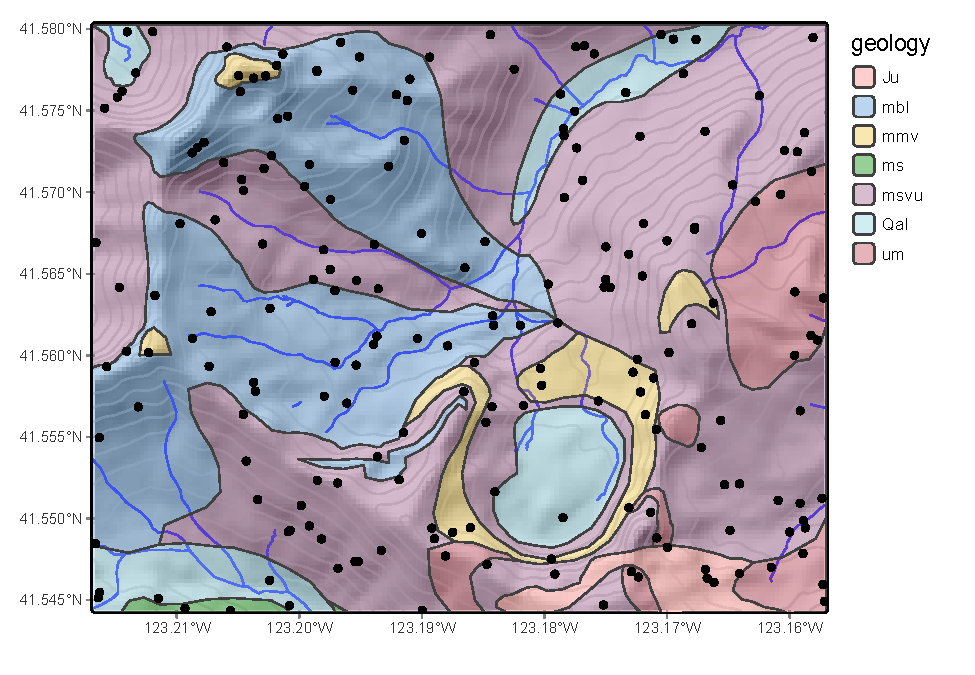
\includegraphics[width=0.75\linewidth]{EnvDataScience_files/figure-latex/rasRandomPtsMarbles-1} 

}

\caption{Random points in the Marble Valley area, Marble Mountains, California}\label{fig:rasRandomPtsMarbles}
\end{figure}

Now we'll extract \index{extraction from rasters}data from each of the rasters, using an S4 version of \texttt{rsamps}, and then bind them together with the \texttt{rsamps} simple features. We'll have to use \texttt{terra::vect} and \texttt{sf::st\_as\_sf} to convert feature data to the type required by specific tools, and due to a function naming issue, we'll need to use the package prefix with \texttt{terra::extract}, but otherwise the code is pretty straightforward.

\begin{Shaded}
\begin{Highlighting}[]
\NormalTok{rsampS4 }\OtherTok{\textless{}{-}} \FunctionTok{vect}\NormalTok{(rsamps)}
\NormalTok{elev\_ex }\OtherTok{\textless{}{-}}\NormalTok{ terra}\SpecialCharTok{::}\FunctionTok{extract}\NormalTok{(elev, rsampS4)     }\SpecialCharTok{|\textgreater{}}\NormalTok{ dplyr}\SpecialCharTok{::}\FunctionTok{select}\NormalTok{(}\SpecialCharTok{{-}}\NormalTok{ID)}
\NormalTok{slope\_ex }\OtherTok{\textless{}{-}}\NormalTok{ terra}\SpecialCharTok{::}\FunctionTok{extract}\NormalTok{(slope, rsampS4)   }\SpecialCharTok{|\textgreater{}}\NormalTok{ dplyr}\SpecialCharTok{::}\FunctionTok{select}\NormalTok{(}\SpecialCharTok{{-}}\NormalTok{ID)}
\NormalTok{geol\_ex }\OtherTok{\textless{}{-}}\NormalTok{ terra}\SpecialCharTok{::}\FunctionTok{extract}\NormalTok{(geol, rsampS4)     }\SpecialCharTok{|\textgreater{}}\NormalTok{ dplyr}\SpecialCharTok{::}\FunctionTok{select}\NormalTok{(}\SpecialCharTok{{-}}\NormalTok{ID)}
\NormalTok{strD\_ex }\OtherTok{\textless{}{-}}\NormalTok{ terra}\SpecialCharTok{::}\FunctionTok{extract}\NormalTok{(str\_dist, rsampS4) }\SpecialCharTok{|\textgreater{}}\NormalTok{ dplyr}\SpecialCharTok{::}\FunctionTok{select}\NormalTok{(}\SpecialCharTok{{-}}\NormalTok{ID)}
\NormalTok{rsampsData }\OtherTok{\textless{}{-}} \FunctionTok{bind\_cols}\NormalTok{(rsamps, elev\_ex, slope\_ex, geol\_ex, strD\_ex)}
\end{Highlighting}
\end{Shaded}

Then plot the map with the points colored by geology (Figure \ref{fig:rasExtractedGeology})\ldots{}

\begin{Shaded}
\begin{Highlighting}[]
\NormalTok{marblesTemplate }\SpecialCharTok{+} 
  \FunctionTok{tm\_shape}\NormalTok{(rsampsData) }\SpecialCharTok{+} \FunctionTok{tm\_dots}\NormalTok{(}\AttributeTok{fill=}\StringTok{"geology"}\NormalTok{, }\AttributeTok{size=}\FloatTok{0.4}\NormalTok{,}\AttributeTok{fill.legend=}\FunctionTok{tm\_legend}\NormalTok{(}\AttributeTok{frame=}\NormalTok{F))}
\end{Highlighting}
\end{Shaded}

\begin{figure}

{\centering 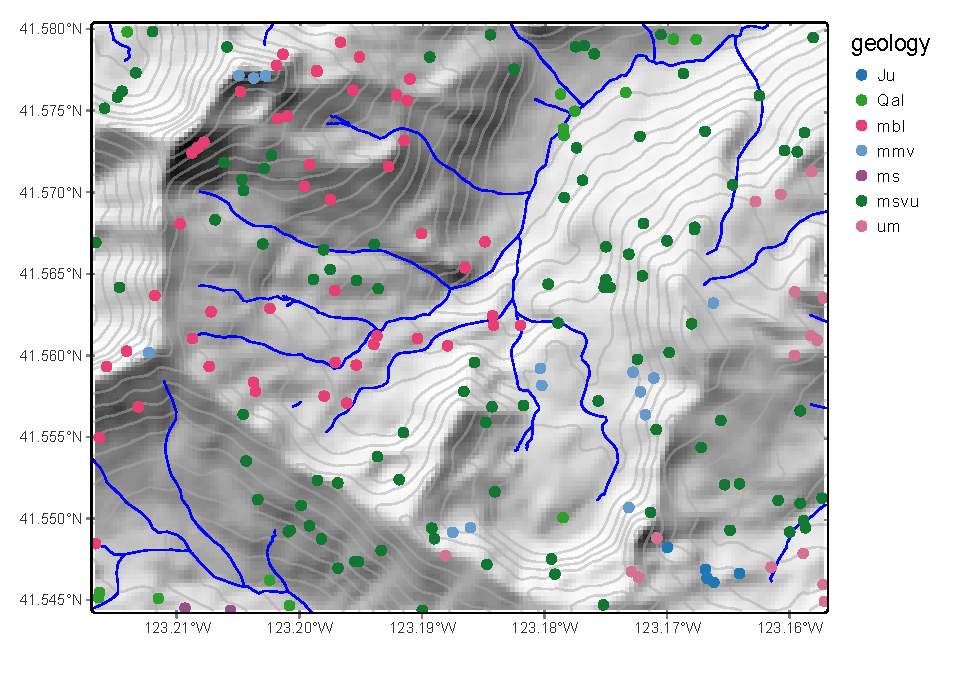
\includegraphics[width=0.75\linewidth]{EnvDataScience_files/figure-latex/rasExtractedGeology-1} 

}

\caption{Points colored by geology extracted from raster}\label{fig:rasExtractedGeology}
\end{figure}

\ldots{} and finally \texttt{str\_dist} by \texttt{elev}, colored by \texttt{geology}, derived by extracting. We'll filter out the NAs along the edge (Figure \ref{fig:rasElevByStrDist}). Of course other analyses and visualizations are possible.

\begin{Shaded}
\begin{Highlighting}[]
\NormalTok{rsampsData }\SpecialCharTok{|\textgreater{}}
  \FunctionTok{filter}\NormalTok{(}\SpecialCharTok{!}\FunctionTok{is.na}\NormalTok{(geology)) }\SpecialCharTok{|\textgreater{}} 
  \FunctionTok{ggplot}\NormalTok{(}\FunctionTok{aes}\NormalTok{(}\AttributeTok{x=}\NormalTok{str\_dist,}\AttributeTok{y=}\NormalTok{elev,}\AttributeTok{col=}\NormalTok{geology)) }\SpecialCharTok{+} 
  \FunctionTok{geom\_point}\NormalTok{() }\SpecialCharTok{+} \FunctionTok{geom\_smooth}\NormalTok{(}\AttributeTok{method =} \StringTok{"lm"}\NormalTok{, }\AttributeTok{se=}\NormalTok{F)}
\end{Highlighting}
\end{Shaded}

\begin{figure}

{\centering 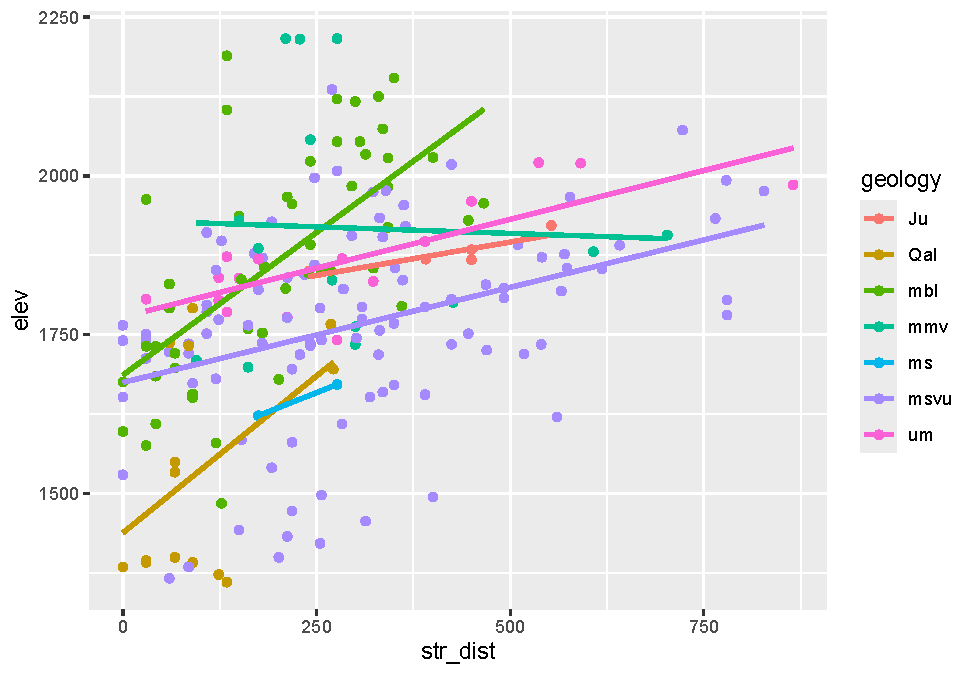
\includegraphics[width=0.75\linewidth]{EnvDataScience_files/figure-latex/rasElevByStrDist-1} 

}

\caption{Elevation by stream distance, colored by geology, random point extraction}\label{fig:rasElevByStrDist}
\end{figure}

Here's a similar example, but using water sample data\index{sample data}, which we can then use to relate to extracted raster values to look at relationships such as in Figures \ref{fig:rasCarbonateGeol}, \ref{fig:rasSlopeElevGeol}, and \ref{fig:rasLogHardness}. It's worthwhile to check various results along the way, as we did above. Most of the code is very similar to what we used above, including dealing with naming the distance rasters.

\begin{Shaded}
\begin{Highlighting}[]
\NormalTok{streams }\OtherTok{\textless{}{-}} \FunctionTok{vect}\NormalTok{(}\FunctionTok{ex}\NormalTok{(}\StringTok{"marbles/streams.shp"}\NormalTok{))}
\NormalTok{trails }\OtherTok{\textless{}{-}} \FunctionTok{vect}\NormalTok{(}\FunctionTok{ex}\NormalTok{(}\StringTok{"marbles/trails.shp"}\NormalTok{))}
\NormalTok{elev }\OtherTok{\textless{}{-}} \FunctionTok{rast}\NormalTok{(}\FunctionTok{ex}\NormalTok{(}\StringTok{"marbles/elev.tif"}\NormalTok{)) }
\NormalTok{geology }\OtherTok{\textless{}{-}} \FunctionTok{st\_read}\NormalTok{(}\FunctionTok{ex}\NormalTok{(}\StringTok{"marbles/geology.shp"}\NormalTok{)) }\SpecialCharTok{|\textgreater{}}
           \FunctionTok{rename}\NormalTok{(}\AttributeTok{geology=}\NormalTok{CLASS)}
\NormalTok{sampsf }\OtherTok{\textless{}{-}} \FunctionTok{st\_read}\NormalTok{(}\FunctionTok{ex}\NormalTok{(}\StringTok{"marbles/samples.shp"}\NormalTok{)) }\SpecialCharTok{|\textgreater{}} 
\NormalTok{  dplyr}\SpecialCharTok{::}\FunctionTok{select}\NormalTok{(CATOT, MGTOT, PH, TEMP, TDS)}
\NormalTok{samples }\OtherTok{\textless{}{-}} \FunctionTok{vect}\NormalTok{(sampsf) }
\NormalTok{strms }\OtherTok{\textless{}{-}} \FunctionTok{rasterize}\NormalTok{(streams,elev)}
\NormalTok{tr }\OtherTok{\textless{}{-}} \FunctionTok{rasterize}\NormalTok{(trails,elev)}
\NormalTok{geol }\OtherTok{\textless{}{-}} \FunctionTok{rasterize}\NormalTok{(geology,elev,}\AttributeTok{field=}\StringTok{"geology"}\NormalTok{)}
\NormalTok{stdist }\OtherTok{\textless{}{-}}\NormalTok{ terra}\SpecialCharTok{::}\FunctionTok{distance}\NormalTok{(strms); }\FunctionTok{names}\NormalTok{(stdist) }\OtherTok{\textless{}{-}} \StringTok{"stDist"}
\NormalTok{trdist }\OtherTok{\textless{}{-}}\NormalTok{ terra}\SpecialCharTok{::}\FunctionTok{distance}\NormalTok{(tr); }\FunctionTok{names}\NormalTok{(trdist) }\OtherTok{=} \StringTok{"trDist"}
\NormalTok{slope }\OtherTok{\textless{}{-}} \FunctionTok{terrain}\NormalTok{(elev, }\AttributeTok{v=}\StringTok{"slope"}\NormalTok{)}
\NormalTok{aspect }\OtherTok{\textless{}{-}} \FunctionTok{terrain}\NormalTok{(elev, }\AttributeTok{v=}\StringTok{"aspect"}\NormalTok{)}
\NormalTok{elev\_ex }\OtherTok{\textless{}{-}}\NormalTok{ terra}\SpecialCharTok{::}\FunctionTok{extract}\NormalTok{(elev, samples)     }\SpecialCharTok{|\textgreater{}}\NormalTok{ dplyr}\SpecialCharTok{::}\FunctionTok{select}\NormalTok{(}\SpecialCharTok{{-}}\NormalTok{ID)}
\NormalTok{slope\_ex }\OtherTok{\textless{}{-}}\NormalTok{ terra}\SpecialCharTok{::}\FunctionTok{extract}\NormalTok{(slope, samples)   }\SpecialCharTok{|\textgreater{}}\NormalTok{ dplyr}\SpecialCharTok{::}\FunctionTok{select}\NormalTok{(}\SpecialCharTok{{-}}\NormalTok{ID)}
\NormalTok{aspect\_ex }\OtherTok{\textless{}{-}}\NormalTok{ terra}\SpecialCharTok{::}\FunctionTok{extract}\NormalTok{(aspect, samples) }\SpecialCharTok{|\textgreater{}}\NormalTok{ dplyr}\SpecialCharTok{::}\FunctionTok{select}\NormalTok{(}\SpecialCharTok{{-}}\NormalTok{ID)}
\NormalTok{geol\_ex }\OtherTok{\textless{}{-}}\NormalTok{ terra}\SpecialCharTok{::}\FunctionTok{extract}\NormalTok{(geol, samples)     }\SpecialCharTok{|\textgreater{}}\NormalTok{ dplyr}\SpecialCharTok{::}\FunctionTok{select}\NormalTok{(}\SpecialCharTok{{-}}\NormalTok{ID)}
\NormalTok{strD\_ex }\OtherTok{\textless{}{-}}\NormalTok{ terra}\SpecialCharTok{::}\FunctionTok{extract}\NormalTok{(stdist, samples)   }\SpecialCharTok{|\textgreater{}}\NormalTok{ dplyr}\SpecialCharTok{::}\FunctionTok{select}\NormalTok{(}\SpecialCharTok{{-}}\NormalTok{ID)}
\NormalTok{trailD\_ex }\OtherTok{\textless{}{-}}\NormalTok{ terra}\SpecialCharTok{::}\FunctionTok{extract}\NormalTok{(trdist, samples) }\SpecialCharTok{|\textgreater{}}\NormalTok{ dplyr}\SpecialCharTok{::}\FunctionTok{select}\NormalTok{(}\SpecialCharTok{{-}}\NormalTok{ID)}
\NormalTok{samplePts }\OtherTok{\textless{}{-}} \FunctionTok{cbind}\NormalTok{(samples,elev\_ex,slope\_ex,aspect\_ex,geol\_ex,strD\_ex,trailD\_ex)}
\NormalTok{samplePtsDF }\OtherTok{\textless{}{-}} \FunctionTok{as.data.frame}\NormalTok{(samplePts)}
\end{Highlighting}
\end{Shaded}

\begin{Shaded}
\begin{Highlighting}[]
\FunctionTok{head}\NormalTok{(samplePtsDF)}
\end{Highlighting}
\end{Shaded}

\begin{verbatim}
##   CATOT MGTOT   PH TEMP  TDS elev     slope     aspect geology   stDist
## 1  0.80  0.02 7.74 15.3 0.16 1357  1.721006 123.690068     Qal   0.0000
## 2  0.83  0.04 7.88 14.8 0.16 1359  6.926249 337.833654     Qal  30.0000
## 3  0.83  0.04 7.47 15.1 0.12 1361  4.222687 106.389540     Qal   0.0000
## 4  0.63  0.03 7.54 15.8 0.17 1356  2.160789 353.659808     Qal   0.0000
## 5  0.67  0.06 7.67 14.0 0.14 1374  1.687605  81.869898     Qal   0.0000
## 6  0.70  0.04 7.35  7.0 0.16 1399 12.713997   4.236395    msvu 192.0937
##     trDist
## 1 169.7056
## 2 318.9044
## 3 108.1665
## 4 241.8677
## 5 150.0000
## 6 342.0526
\end{verbatim}

\begin{Shaded}
\begin{Highlighting}[]
\FunctionTok{ggplot}\NormalTok{(}\AttributeTok{data=}\NormalTok{samplePtsDF, }\FunctionTok{aes}\NormalTok{(}\AttributeTok{x=}\NormalTok{geology,}\AttributeTok{y=}\NormalTok{CATOT)) }\SpecialCharTok{+} \FunctionTok{geom\_boxplot}\NormalTok{()}
\end{Highlighting}
\end{Shaded}

\begin{figure}

{\centering 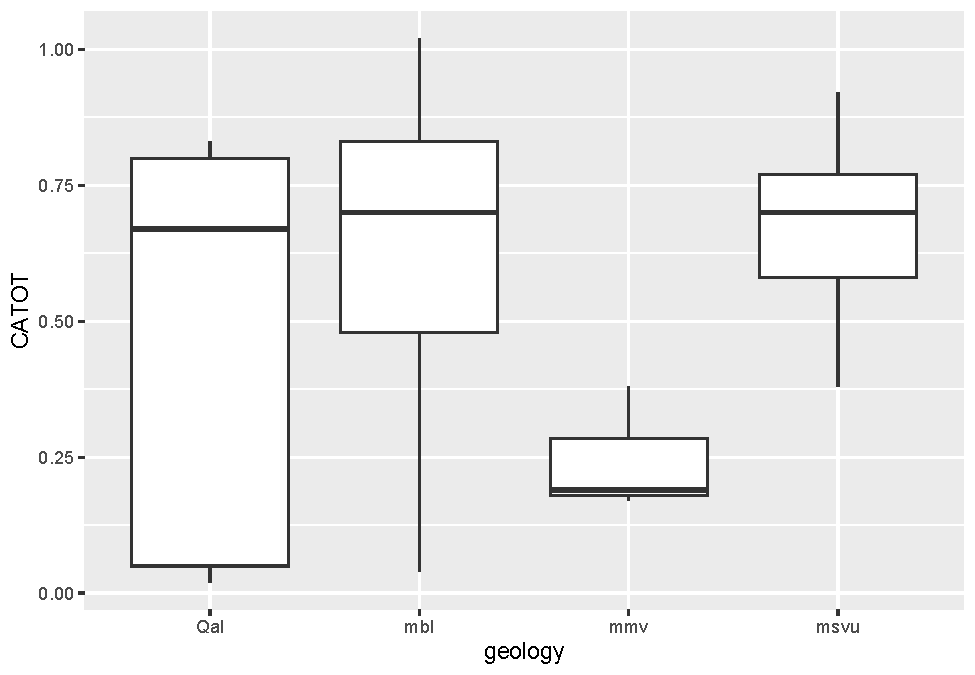
\includegraphics[width=0.75\linewidth]{EnvDataScience_files/figure-latex/rasCarbonateGeol-1} 

}

\caption{Dissolved calcium carbonate grouped by geology extracted at water sample points}\label{fig:rasCarbonateGeol}
\end{figure}

\begin{Shaded}
\begin{Highlighting}[]
\FunctionTok{ggplot}\NormalTok{(}\AttributeTok{data=}\NormalTok{samplePtsDF, }\FunctionTok{aes}\NormalTok{(}\AttributeTok{x=}\NormalTok{slope,}\AttributeTok{y=}\NormalTok{elev,}\AttributeTok{col=}\NormalTok{geology)) }\SpecialCharTok{+} \FunctionTok{geom\_point}\NormalTok{()}
\end{Highlighting}
\end{Shaded}

\begin{figure}

{\centering 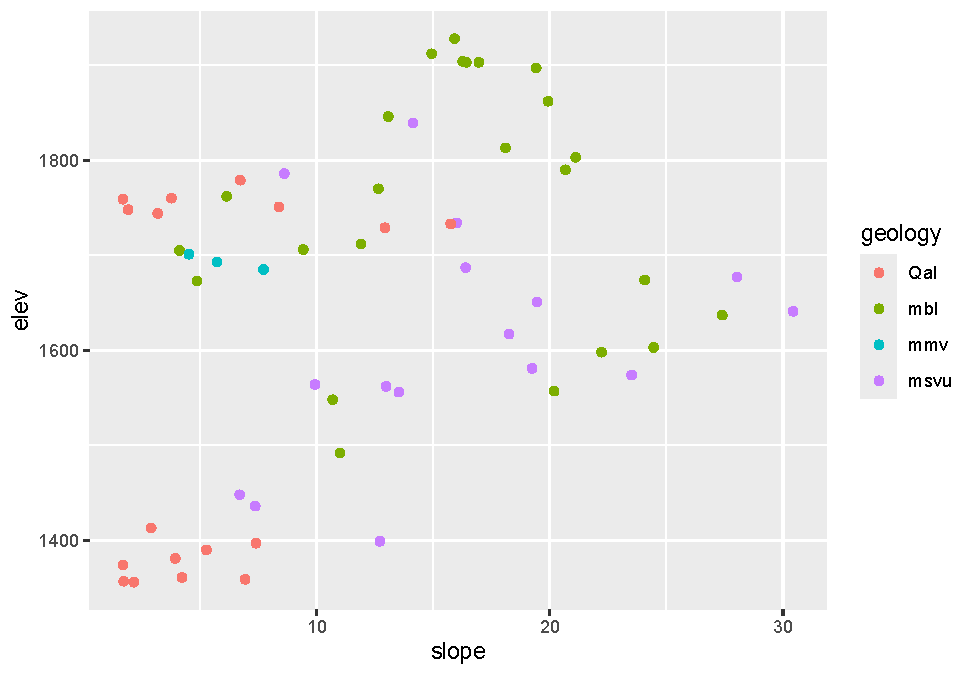
\includegraphics[width=0.75\linewidth]{EnvDataScience_files/figure-latex/rasSlopeElevGeol-1} 

}

\caption{Slope by elevation colored by extracted geology}\label{fig:rasSlopeElevGeol}
\end{figure}

\begin{Shaded}
\begin{Highlighting}[]
\NormalTok{cont }\OtherTok{\textless{}{-}} \FunctionTok{st\_as\_sf}\NormalTok{(}\FunctionTok{as.contour}\NormalTok{(elev, }\AttributeTok{nlevels=}\DecValTok{30}\NormalTok{))}
\end{Highlighting}
\end{Shaded}

\begin{Shaded}
\begin{Highlighting}[]
\NormalTok{marblesTemplate }\SpecialCharTok{+}
  \FunctionTok{tm\_shape}\NormalTok{(geolshp) }\SpecialCharTok{+} \FunctionTok{tm\_polygons}\NormalTok{(}\AttributeTok{fill=}\StringTok{"geology"}\NormalTok{, }\AttributeTok{fill\_alpha=}\FloatTok{0.5}\NormalTok{, }\AttributeTok{fill.legend=}\FunctionTok{tm\_legend}\NormalTok{(}\AttributeTok{frame=}\NormalTok{F)) }\SpecialCharTok{+}
  \FunctionTok{tm\_shape}\NormalTok{(sampsf) }\SpecialCharTok{+} \FunctionTok{tm\_dots}\NormalTok{(}\AttributeTok{size=}\StringTok{"CATOT"}\NormalTok{)}
\end{Highlighting}
\end{Shaded}

\begin{figure}

{\centering 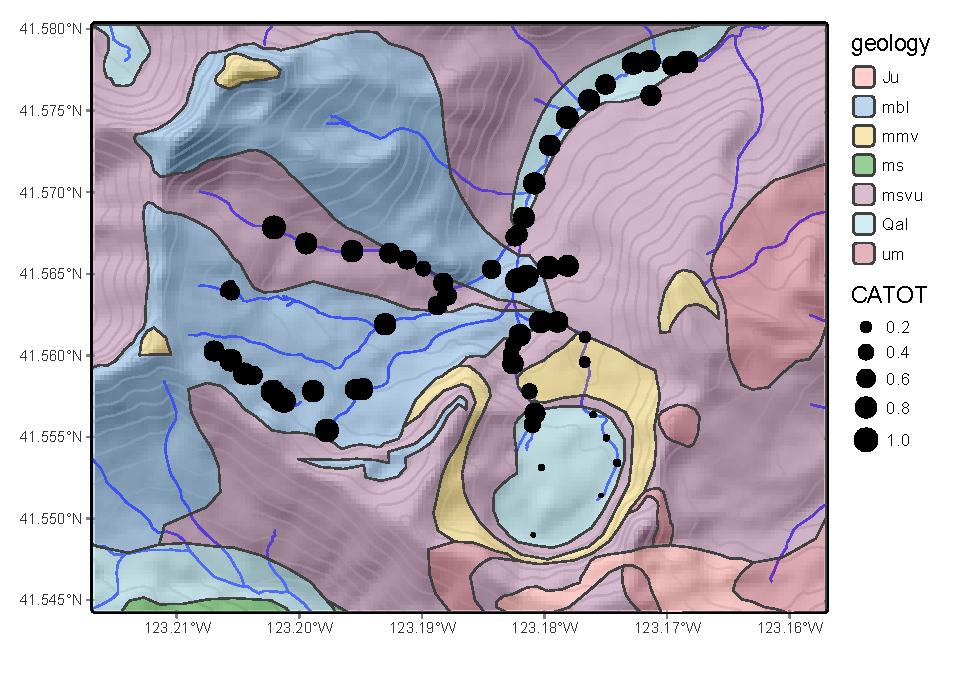
\includegraphics[width=0.75\linewidth]{EnvDataScience_files/figure-latex/rasLogHardness-1} 

}

\caption{Calcium carbonate total hardness at sample points, showing geologic units}\label{fig:rasLogHardness}
\end{figure}

\section{Focal Statistics}\label{focal-statistics}

\index{focal statistics}Focal (or neighborhood\index{neighborhood statistics}) statistics work with a continuous or categorical raster to pass a moving window through it, assigning the central cell with summary statistic applied to the neighborhood, which by default is a \(3\times3\) neighborhood (\texttt{w=3}) centered on the cell. One of the simplest is a low-pass filter where \texttt{fun="mean"}. This applied to a continuous raster like elevation will look very similar to the original, so we'll apply a larger \(9\times9\) (\texttt{w=9}) window \index{low-pass filter}so we can see the effect (Figure \ref{fig:rasFocalMean}), which you can compare with the earlier plots of raw elevation.

\begin{Shaded}
\begin{Highlighting}[]
\NormalTok{elevLowPass9 }\OtherTok{\textless{}{-}}\NormalTok{ terra}\SpecialCharTok{::}\FunctionTok{focal}\NormalTok{(elev,}\AttributeTok{w=}\DecValTok{9}\NormalTok{,}\AttributeTok{fun=}\StringTok{"mean"}\NormalTok{)}
\FunctionTok{names}\NormalTok{(elevLowPass9) }\OtherTok{\textless{}{-}} \StringTok{"elevLowPass9"} \CommentTok{\# otherwise gets "elev"}
\FunctionTok{plot}\NormalTok{(elevLowPass9)}
\end{Highlighting}
\end{Shaded}

\begin{figure}

{\centering 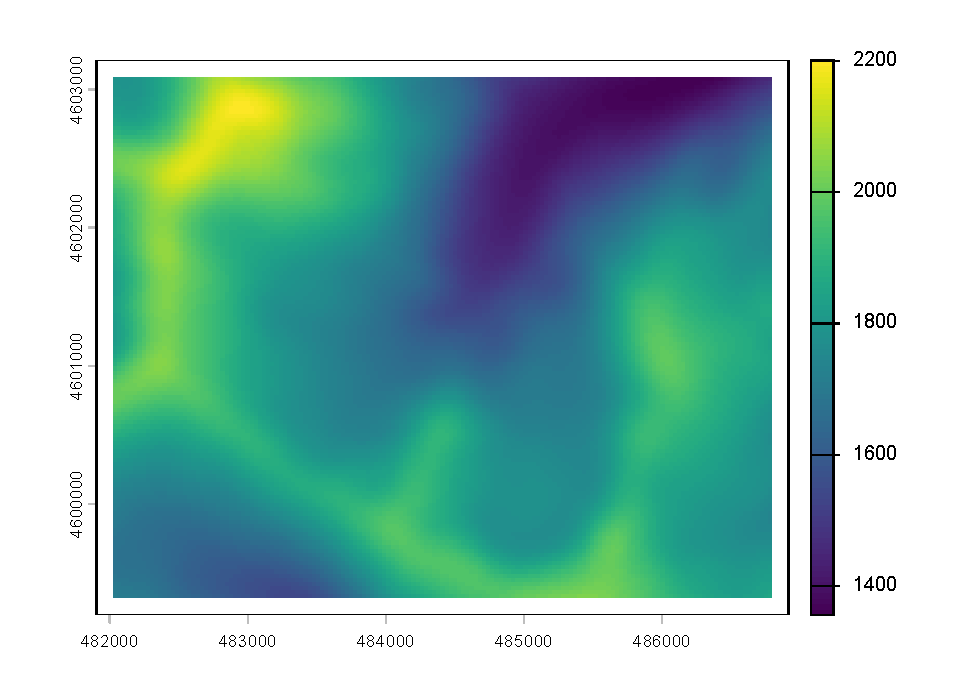
\includegraphics[width=0.75\linewidth]{EnvDataScience_files/figure-latex/rasFocalMean-1} 

}

\caption{9x9 focal mean of elevation}\label{fig:rasFocalMean}
\end{figure}

The effect is probably much more apparent in a hillshade, where the very smooth 9x9 low-pass filtered elevation will seem to create an out-of-focus hillshade (Figure \ref{fig:rasHillshFocalMean}).

\begin{Shaded}
\begin{Highlighting}[]
\NormalTok{slope9 }\OtherTok{\textless{}{-}} \FunctionTok{terrain}\NormalTok{(elevLowPass9, }\AttributeTok{v=}\StringTok{"slope"}\NormalTok{)}
\NormalTok{aspect9 }\OtherTok{\textless{}{-}} \FunctionTok{terrain}\NormalTok{(elevLowPass9, }\AttributeTok{v=}\StringTok{"aspect"}\NormalTok{)}
\FunctionTok{plot}\NormalTok{(}\FunctionTok{shade}\NormalTok{(slope9}\SpecialCharTok{/}\DecValTok{180}\SpecialCharTok{*}\NormalTok{pi, aspect9}\SpecialCharTok{/}\DecValTok{180}\SpecialCharTok{*}\NormalTok{pi, }\AttributeTok{angle=}\DecValTok{40}\NormalTok{, }\AttributeTok{direction=}\DecValTok{330}\NormalTok{),}
     \AttributeTok{col=}\FunctionTok{gray}\NormalTok{(}\DecValTok{0}\SpecialCharTok{:}\DecValTok{100}\SpecialCharTok{/}\DecValTok{100}\NormalTok{))}
\end{Highlighting}
\end{Shaded}

\begin{figure}

{\centering 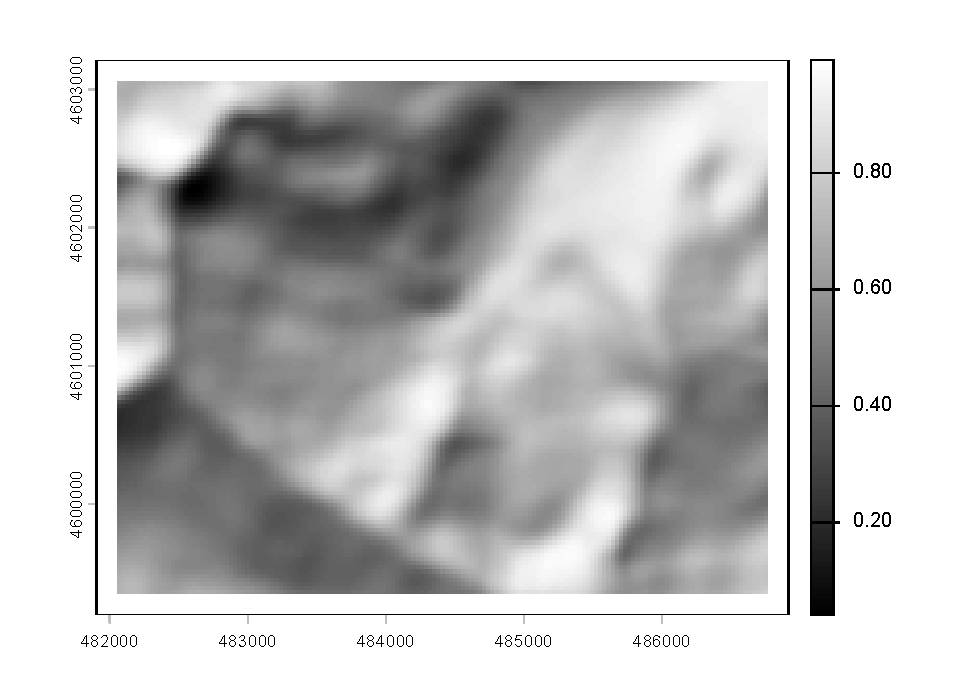
\includegraphics[width=0.75\linewidth]{EnvDataScience_files/figure-latex/rasHillshFocalMean-1} 

}

\caption{Hillshade of 9x9 focal mean of elevation}\label{fig:rasHillshFocalMean}
\end{figure}

For categorical/factor data such as geology (Figure \ref{fig:rasMblGeol}), the modal class in the neighborhood \index{focal modal value for categorical rasters}can be defined (Figure \ref{fig:rasModalGeol}).

\begin{Shaded}
\begin{Highlighting}[]
\FunctionTok{plot}\NormalTok{(geol)}
\end{Highlighting}
\end{Shaded}

\begin{figure}

{\centering 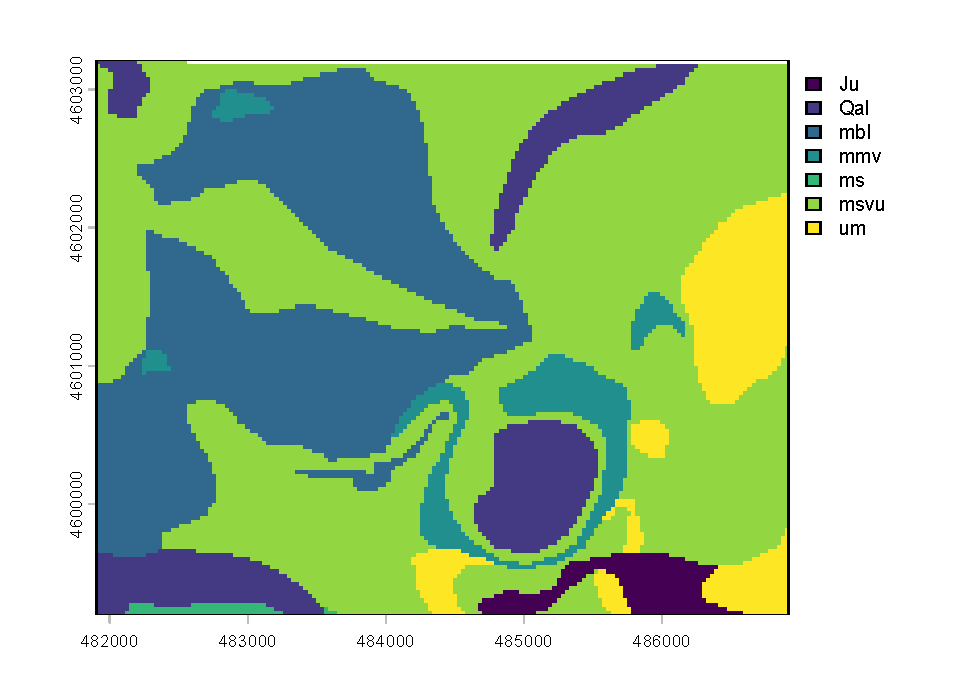
\includegraphics[width=0.75\linewidth]{EnvDataScience_files/figure-latex/rasMblGeol-1} 

}

\caption{Marble Mountains geology raster}\label{fig:rasMblGeol}
\end{figure}

\begin{Shaded}
\begin{Highlighting}[]
\FunctionTok{library}\NormalTok{(tmap)}
\FunctionTok{tm\_shape}\NormalTok{(geol) }\SpecialCharTok{+} \FunctionTok{tm\_raster}\NormalTok{()}
\end{Highlighting}
\end{Shaded}

\begin{center}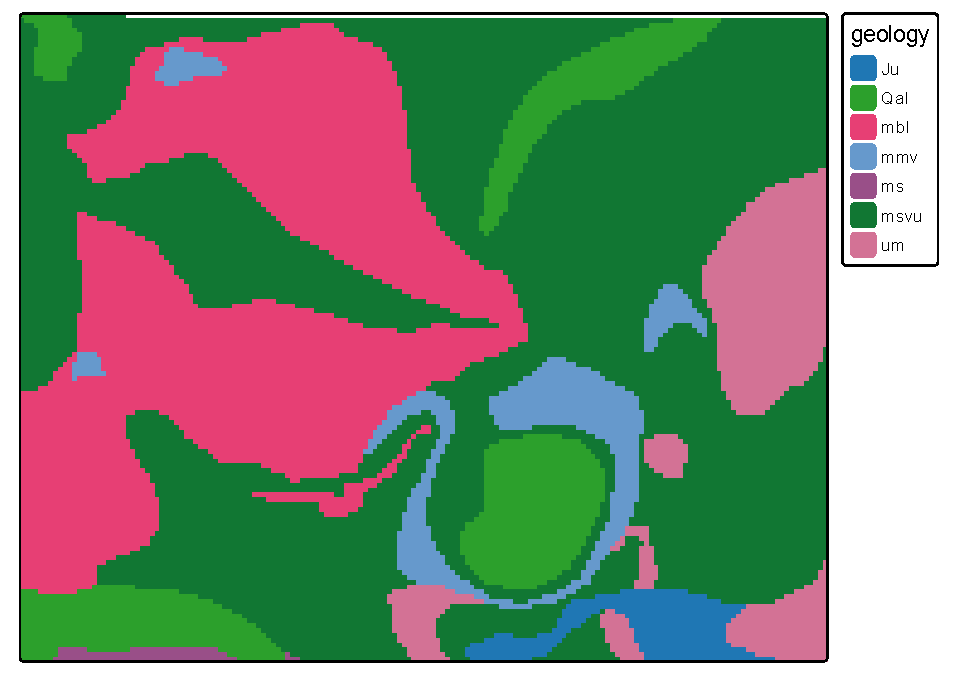
\includegraphics[width=0.75\linewidth]{EnvDataScience_files/figure-latex/unnamed-chunk-236-1} \end{center}

\begin{Shaded}
\begin{Highlighting}[]
\FunctionTok{plot}\NormalTok{(terra}\SpecialCharTok{::}\FunctionTok{focal}\NormalTok{(geol,}\AttributeTok{w=}\DecValTok{9}\NormalTok{,}\AttributeTok{fun=}\StringTok{"modal"}\NormalTok{))}
\end{Highlighting}
\end{Shaded}

\begin{figure}

{\centering 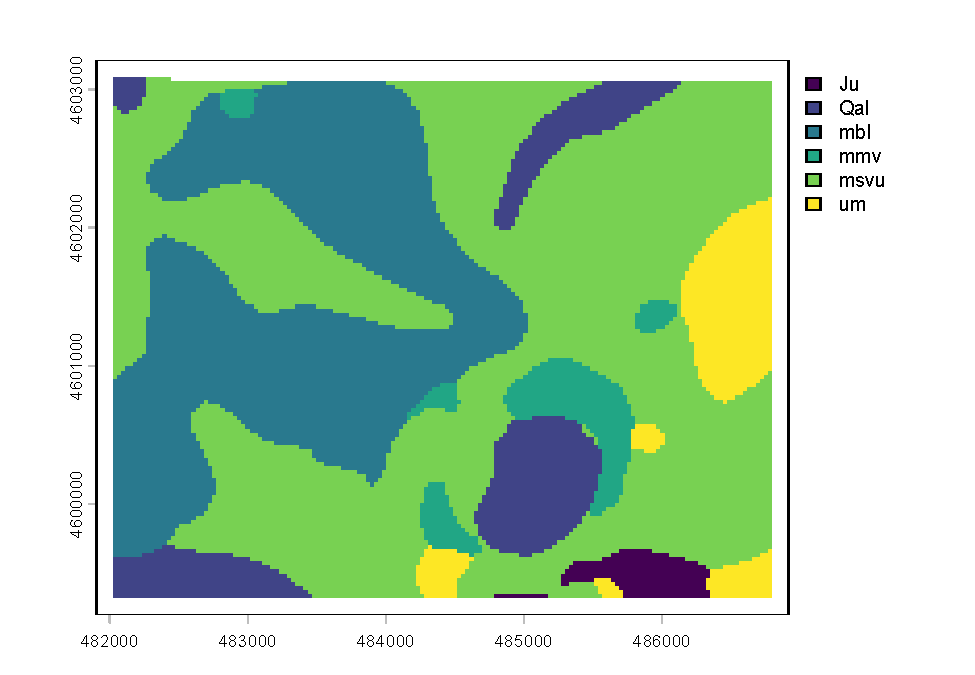
\includegraphics[width=0.75\linewidth]{EnvDataScience_files/figure-latex/rasModalGeol-1} 

}

\caption{Modal geology in 9 by 9 neighborhoods}\label{fig:rasModalGeol}
\end{figure}

Note that while plot displayed these with a continuous legend, the modal result is going to be an integer value representing the modal class, the most common rock type in the neighborhood. This is sometimes called a \emph{majority filter}. \emph{Challenge}: how could we link the modes to the original character \texttt{geology} value, and produce a more useful map?

\section{Zonal Statistics}\label{zonal-statistics}

\index{zonal statistics}Zonal statistics let you stratify by zone, and is a lot like the grouped summary (\ref{group-summary}) we've done before, but in this case the groups are connected to the input raster values by location. There's probably a more elegant way of doing this, but here are a few that are then joined together.

\begin{Shaded}
\begin{Highlighting}[]
\NormalTok{meanElev }\OtherTok{\textless{}{-}} \FunctionTok{zonal}\NormalTok{(elev,geol,}\StringTok{"mean"}\NormalTok{) }\SpecialCharTok{|\textgreater{}} \FunctionTok{rename}\NormalTok{(}\AttributeTok{mean=}\NormalTok{elev)}
\NormalTok{maxElev }\OtherTok{\textless{}{-}} \FunctionTok{zonal}\NormalTok{(elev,geol,}\StringTok{"max"}\NormalTok{)   }\SpecialCharTok{|\textgreater{}} \FunctionTok{rename}\NormalTok{(}\AttributeTok{max=}\NormalTok{elev)}
\NormalTok{minElev }\OtherTok{\textless{}{-}} \FunctionTok{zonal}\NormalTok{(elev,geol,}\StringTok{"min"}\NormalTok{)   }\SpecialCharTok{|\textgreater{}} \FunctionTok{rename}\NormalTok{(}\AttributeTok{min=}\NormalTok{elev)}
\end{Highlighting}
\end{Shaded}

\begin{Shaded}
\begin{Highlighting}[]
\FunctionTok{left\_join}\NormalTok{(}\FunctionTok{left\_join}\NormalTok{(meanElev,maxElev,}\AttributeTok{by=}\StringTok{"geology"}\NormalTok{),minElev,}\AttributeTok{by=}\StringTok{"geology"}\NormalTok{)}
\end{Highlighting}
\end{Shaded}

\begin{verbatim}
##   geology     mean  max  min
## 1      Ju 1940.050 2049 1815
## 2     Qal 1622.944 1825 1350
## 3     mbl 1837.615 2223 1463
## 4     mmv 1846.186 2260 1683
## 5      ms 1636.802 1724 1535
## 6    msvu 1750.205 2136 1336
## 7      um 1860.758 2049 1719
\end{verbatim}

\pagebreak

\section{Exercises: Raster Spatial Analysis}\label{exercises-raster-spatial-analysis}

\begin{exercise}
See section 8.4 on deriving the extent of an elevation raster from the Marble Mountains as minimum and maximum x and y values, and of creating uniform random numbers between those limits. Modify this approach to stay away from the edges by about 5\% of the range, and derive 100 points. If you derive xrange and yrange scalars that represent the positive difference between the maximum and minimum values of each, you can work out what the min and max limits are of uniform random numbers that would be 5\% higher than the minimums and 5\% lower than the maximums. Use methods from 3.2.1 to create a data frame \texttt{pts} with x and y columns, and display that data frame.
\end{exercise}

\begin{exercise}
Create sf points from those coordinate pairs in \texttt{pts}, using methods from 6.3, and set their coordinate system to that of the elevation raster, using a method such st\_crs as described in 6.2, which illustrates features but the same applies to rasters. Then use tmap to display them on a base of the elevation raster.
\end{exercise}

\begin{center}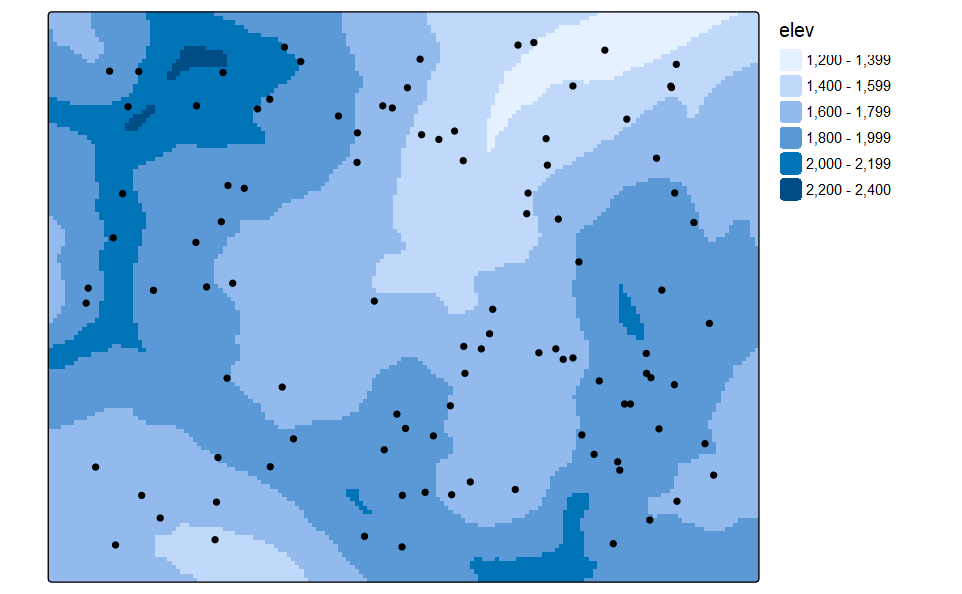
\includegraphics[width=0.75\linewidth]{img/ras_ex2} \end{center}

\begin{exercise}
\textbf{Geology and elevation by stream and trail distance}. Now use those points to extract values from stream distance, trail distance, geology, slope, aspect, and elevation, and display that sf data frame as a table, then plot trail distance (x) vs stream distance (y) colored by geology and sized by elevation (Figure \ref{fig:rasGeolElevDistGoal}).
\end{exercise}

\begin{figure}

{\centering 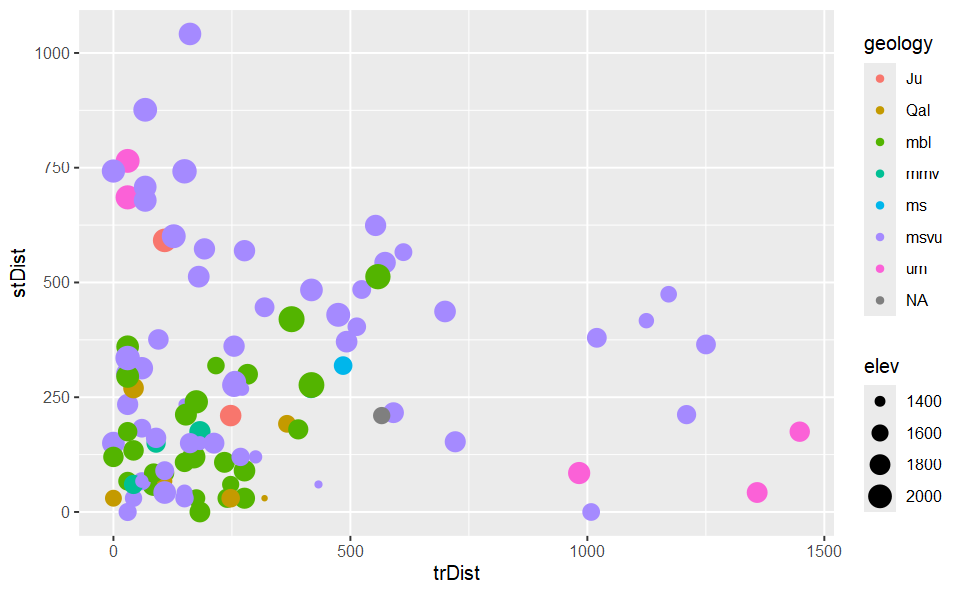
\includegraphics[width=0.75\linewidth]{img/ras_ex3} 

}

\caption{Geology and elevation by stream and trail distance (goal)}\label{fig:rasGeolElevDistGoal}
\end{figure}

\begin{exercise}
Create a slope raster from the dem TIFF in the SanPedro folder in igisci, then a ``steep'' raster of all slopes \textgreater{} 26 degrees, determined by a study of landslides to be a common landslide threshold, then display them along with roads ``SanPedro/roads.shp'' in ``black'', streams ``SanPedro/streams.shp'' in ``blue'', and watershed borders ``SanPedro/SPCWatershed.shp'' in ``darkgreen'' with lwd=2, using methods from 8.2, figure 8.9.
\end{exercise}

\begin{center}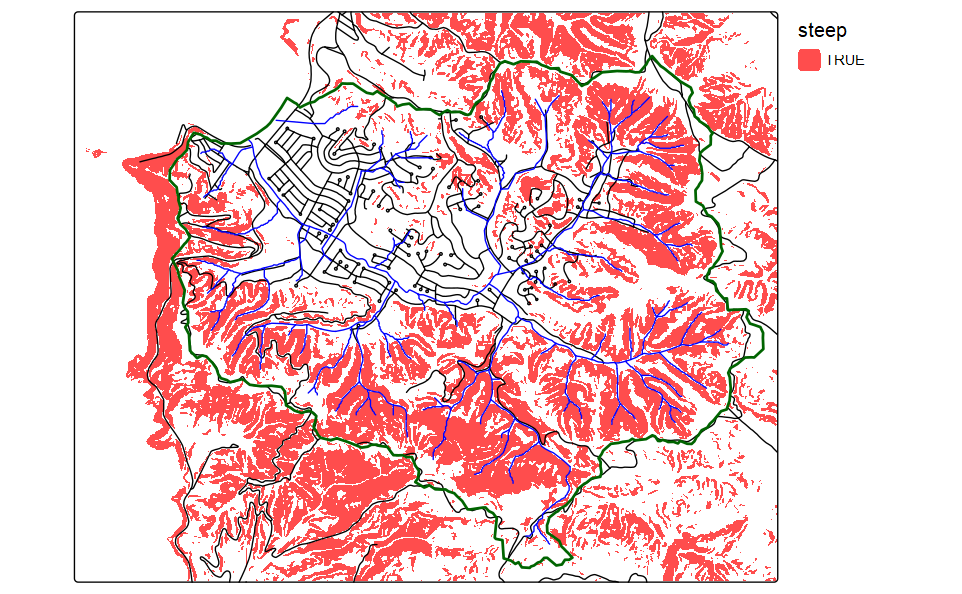
\includegraphics[width=0.75\linewidth]{img/ras_ex4} \end{center}

\begin{exercise}
Add a hillshade to that map.
\end{exercise}

\begin{center}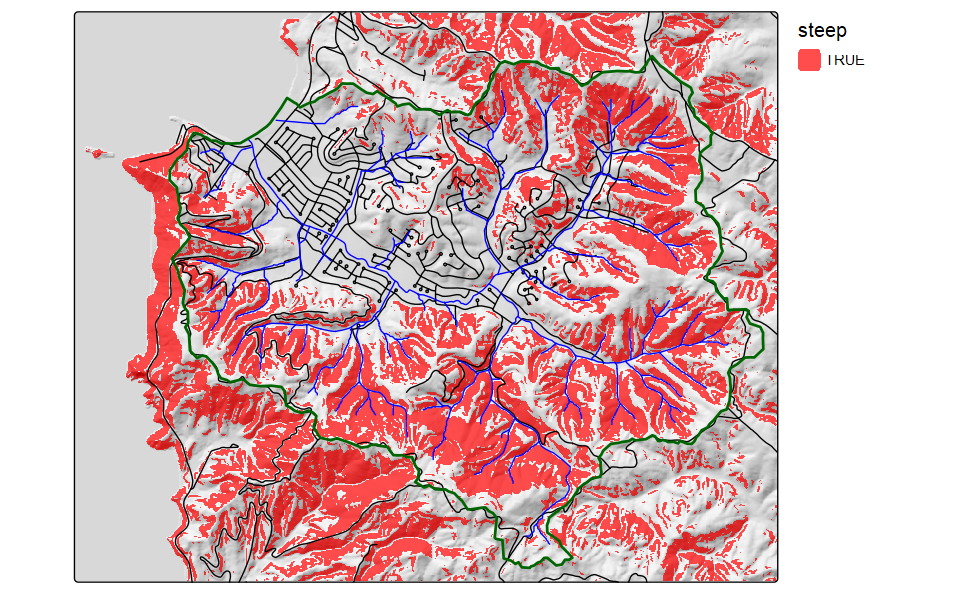
\includegraphics[width=0.75\linewidth]{img/ras_ex5} \end{center}

\part{Statistics and Modeling}\label{part-statistics-and-modeling}

\chapter{Statistical Summaries and Tests}\label{statistics}

\begin{center}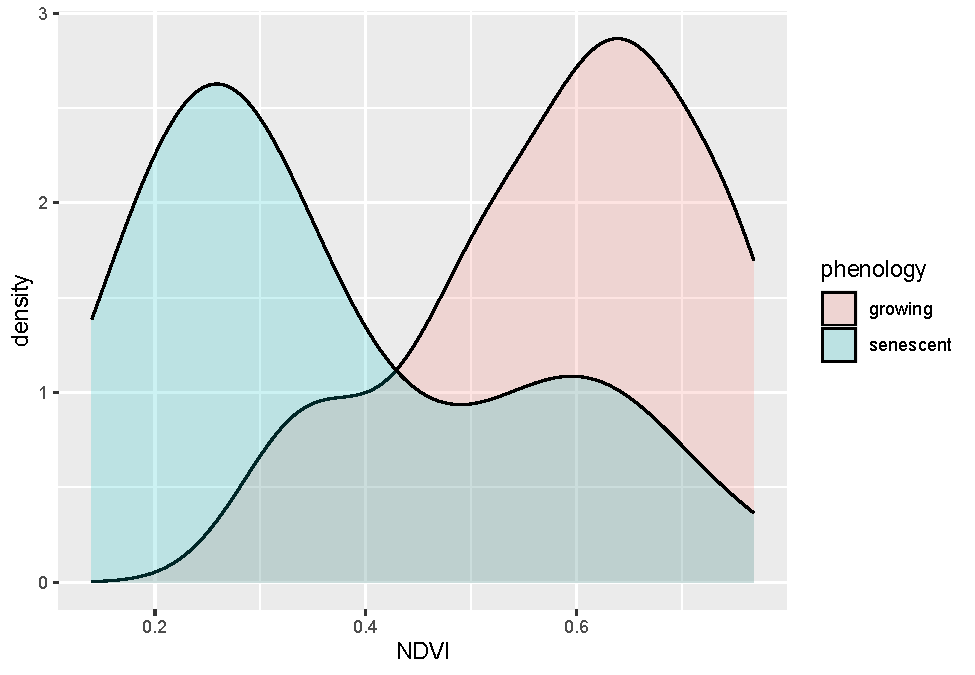
\includegraphics[width=0.75\linewidth]{EnvDataScience_files/figure-latex/StatSummariesTestsChapter-1} \end{center}

\section{Goals of Statistical Analysis}\label{goals-of-statistical-analysis}

\index{statistical analysis}To frame how we might approach statistical analysis and modeling, there are various goals that are commonly involved:

\begin{itemize}
\item
  To understand our data

  \begin{itemize}
  \tightlist
  \item
    nature of our data, through summary statistics and various graphics like histograms
  \item
    spatial statistical analysis
  \item
    time series analysis
  \end{itemize}
\item
  To \emph{group} or \emph{classify} things based on their properties

  \begin{itemize}
  \tightlist
  \item
    using factors to define groups, and deriving grouped summaries
  \item
    comparing \emph{observed} vs \emph{expected} counts or probabilities
  \end{itemize}
\item
  To understand how variables relate to one another

  \begin{itemize}
  \tightlist
  \item
    or maybe even explain variations in other variables, through correlation analysis
  \end{itemize}
\item
  To \emph{model} behavior and maybe \emph{predict} it

  \begin{itemize}
  \tightlist
  \item
    various linear models
  \end{itemize}
\item
  To \emph{confirm} our observations from exploration (field/lab/vis)

  \begin{itemize}
  \tightlist
  \item
    inferential statistics e.g.~difference of means tests, ANOVA, \(\chi^2\)
  \end{itemize}
\item
  To have the confidence to draw conclusions, make informed decisions
\item
  To help \emph{communicate} our work
\end{itemize}

These goals can be seen in the context of a typical research paper or thesis outline in environmental science:

\begin{itemize}
\item
  Introduction
\item
  Literature Review
\item
  Methodology
\item
  Results

  \begin{itemize}
  \tightlist
  \item
    field, lab, geospatial data
  \end{itemize}
\item
  Analysis

  \begin{itemize}
  \tightlist
  \item
    statistical analysis
  \item
    qualitative analysis
  \item
    visualization
  \end{itemize}
\item
  Discussion

  \begin{itemize}
  \tightlist
  \item
    making sense of analysis
  \item
    possibly recursive, with visualization
  \end{itemize}
\item
  Conclusion

  \begin{itemize}
  \tightlist
  \item
    conclusion about what the above shows
  \item
    new questions for further research
  \item
    possible policy recommendation
  \end{itemize}
\end{itemize}

The scope and theory of statistical analysis and models is extensive, and there are many good books on the subject that employ the R language, including sources that focus on environmental topics like water resources (e.g. Helsel et al. (\citeproc{ref-StatisticalMethodsWaterResources}{2020})). This chapter is a short review of some of these methods and how they apply to environmental data science.

\section{Summary Statistics}\label{summary-statistics}

\index{summary statistics}Summary statistics such as mean, standard deviation, variance, minimum, maximum, and range are derived in quite a few R functions, commonly as a parameter or a sub-function (see \texttt{mutate}). An overall simple statistical summary is very easy to do in base R:

\begin{Shaded}
\begin{Highlighting}[]
\FunctionTok{summary}\NormalTok{(tidy\_eucoak)}
\end{Highlighting}
\end{Shaded}

\begin{verbatim}
##         site         site #             tree          Date           
##  Length   :180   Min.   :1.000   Length   :180   Min.   :2006-11-08  
##  N.unique :  8   1st Qu.:2.000   N.unique :  2   1st Qu.:2006-12-07  
##  N.blank  :  0   Median :4.000   N.blank  :  0   Median :2007-01-30  
##  Min.nchar:  3   Mean   :4.422   Min.nchar:  3   Mean   :2007-01-29  
##  Max.nchar:  3   3rd Qu.:6.000   Max.nchar:  3   3rd Qu.:2007-03-22  
##                  Max.   :8.000                   Max.   :2007-05-07  
##                                                                      
##        month        rain_mm      rain_subcanopy      slope      
##  Length   :180   Min.   : 1.00   Min.   : 1.00   Min.   : 9.00  
##  N.unique :  7   1st Qu.:16.00   1st Qu.:16.00   1st Qu.:12.00  
##  N.blank  :  0   Median :28.50   Median :30.00   Median :24.00  
##  Min.nchar:  8   Mean   :37.99   Mean   :34.84   Mean   :20.48  
##  Max.nchar:  9   3rd Qu.:63.25   3rd Qu.:50.00   3rd Qu.:27.00  
##                  Max.   :99.00   Max.   :98.00   Max.   :32.00  
##                  NAs    :36      NAs    :4                      
##      aspect         runoff_L      surface_tension runoff_rainfall_ratio
##  Min.   :100.0   Min.   : 0.000   Min.   :28.51   Min.   :0.00000      
##  1st Qu.:143.0   1st Qu.: 0.000   1st Qu.:37.40   1st Qu.:0.00000      
##  Median :196.0   Median : 0.825   Median :62.60   Median :0.03347      
##  Mean   :186.6   Mean   : 2.244   Mean   :55.73   Mean   :0.05981      
##  3rd Qu.:221.8   3rd Qu.: 3.200   3rd Qu.:72.75   3rd Qu.:0.08474      
##  Max.   :296.0   Max.   :16.000   Max.   :72.75   Max.   :0.42000      
##                  NAs    :8        NAs    :44      NAs    :8
\end{verbatim}

\subsection{\texorpdfstring{Summarize by group: \emph{stratifying a summary}}{Summarize by group: stratifying a summary}}\label{summarize-by-group-stratifying-a-summary}

\index{grouped summary}\index{stratification}In the visualization chapter and elsewhere, we've seen the value of adding symbolization based on a categorical variable or factor. Summarizing by group has a similar benefit, and provides a tabular output in the form of a data frame, and the tidyverse makes it easy to extract several summary statistics at once. For instance, for the euc/oak study, we can create variables of the mean and maximum runoff, the mean and standard deviation of rainfall, for each of the sites. This table alone provides a useful output, but we can also use it in further analyses.

\begin{Shaded}
\begin{Highlighting}[]
\NormalTok{eucoakrainfallrunoffTDR }\SpecialCharTok{\%\textgreater{}\%}
  \FunctionTok{group\_by}\NormalTok{(site) }\SpecialCharTok{\%\textgreater{}\%}
  \FunctionTok{summarize}\NormalTok{(}
    \AttributeTok{rain =} \FunctionTok{mean}\NormalTok{(rain\_mm, }\AttributeTok{na.rm =} \ConstantTok{TRUE}\NormalTok{),}
    \AttributeTok{rainSD =} \FunctionTok{sd}\NormalTok{(rain\_mm, }\AttributeTok{na.rm =} \ConstantTok{TRUE}\NormalTok{),}
    \AttributeTok{runoffL\_oak =} \FunctionTok{mean}\NormalTok{(runoffL\_oak, }\AttributeTok{na.rm =} \ConstantTok{TRUE}\NormalTok{),}
    \AttributeTok{runoffL\_euc =} \FunctionTok{mean}\NormalTok{(runoffL\_euc, }\AttributeTok{na.rm =} \ConstantTok{TRUE}\NormalTok{),}
    \AttributeTok{runoffL\_oakMax =} \FunctionTok{max}\NormalTok{(runoffL\_oak, }\AttributeTok{na.rm =} \ConstantTok{TRUE}\NormalTok{),}
    \AttributeTok{runoffL\_eucMax =} \FunctionTok{max}\NormalTok{(runoffL\_euc, }\AttributeTok{na.rm =} \ConstantTok{TRUE}\NormalTok{),}
\NormalTok{  )}
\end{Highlighting}
\end{Shaded}

\begin{verbatim}
## # A tibble: 8 x 7
##   site   rain rainSD runoffL_oak runoffL_euc runoffL_oakMax runoffL_eucMax
##   <chr> <dbl>  <dbl>       <dbl>       <dbl>          <dbl>          <dbl>
## 1 AB1    48.4   28.2      6.80         6.03          6.80            6.03 
## 2 AB2    34.1   27.9      4.91         3.65          4.91            3.65 
## 3 KM1    48     32.0      1.94         0.592         1.94            0.592
## 4 PR1    56.5   19.1      0.459        2.31          0.459           2.31 
## 5 TP1    38.4   29.5      0.877        1.66          0.877           1.66 
## 6 TP2    34.3   29.2      0.0955       1.53          0.0955          1.53 
## 7 TP3    32.1   28.4      0.381        0.815         0.381           0.815
## 8 TP4    32.5   28.2      0.231        2.83          0.231           2.83
\end{verbatim}

\subsection{Boxplot for visualizing distributions by group}\label{boxplot-for-visualizing-distributions-by-group}

\index{boxplots by group}We've looked at this already in the visualization chapter, but a Tukey boxplot is a good way to visualize distributions by group. In this soil CO\textsubscript{2} study of the Marble Mountains (\citeproc{ref-marblesCO2}{Davis et al. 2001}) (Figure \ref{fig:statTukey}), some sites had much greater variance, and some sites tended to be low vs high (Figure \ref{fig:statCO2avgbysite}).

\begin{Shaded}
\begin{Highlighting}[]
\NormalTok{soilCO2\_97}\SpecialCharTok{$}\NormalTok{SITE }\OtherTok{\textless{}{-}} \FunctionTok{factor}\NormalTok{(soilCO2\_97}\SpecialCharTok{$}\NormalTok{SITE)}
\FunctionTok{ggplot}\NormalTok{(}\AttributeTok{data =}\NormalTok{ soilCO2\_97, }\AttributeTok{mapping =} \FunctionTok{aes}\NormalTok{(}\AttributeTok{x =}\NormalTok{ SITE, }\AttributeTok{y =}\NormalTok{ CO2pct)) }\SpecialCharTok{+}
  \FunctionTok{geom\_boxplot}\NormalTok{()}
\end{Highlighting}
\end{Shaded}

\begin{figure}

{\centering 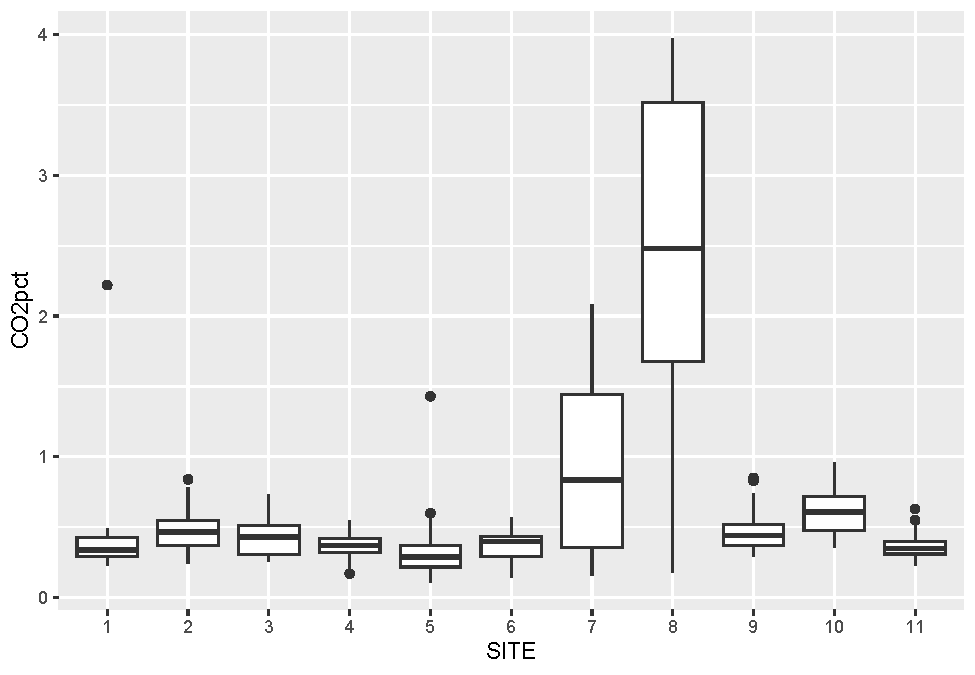
\includegraphics[width=0.75\linewidth]{EnvDataScience_files/figure-latex/statTukey-1} 

}

\caption{Tukey boxplot by group}\label{fig:statTukey}
\end{figure}

\begin{figure}

{\centering 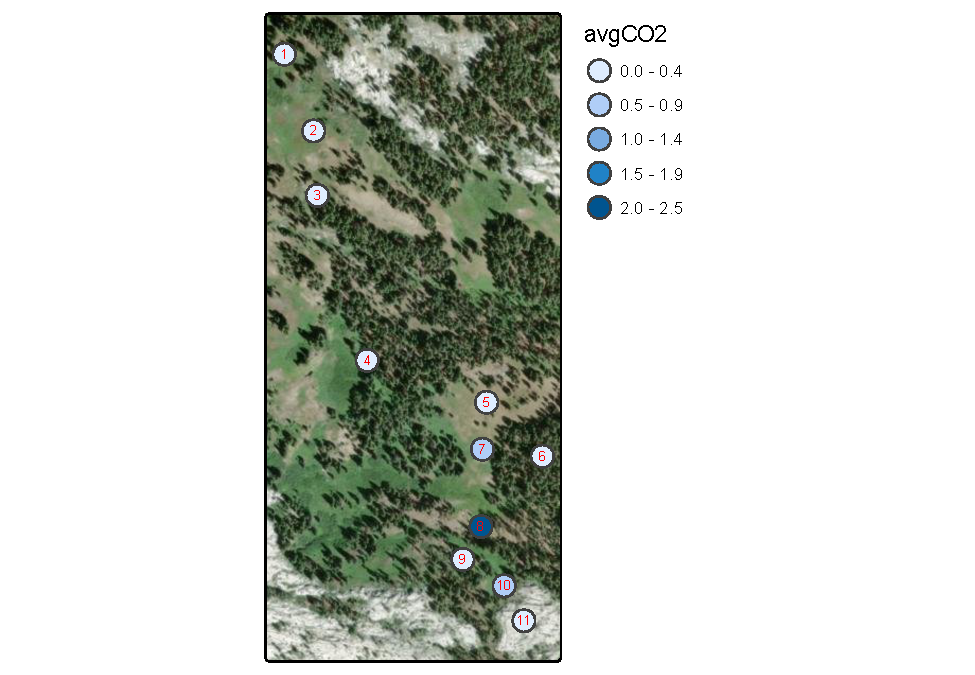
\includegraphics[width=0.75\linewidth]{EnvDataScience_files/figure-latex/statCO2avgbysite-1} 

}

\caption{Marble Mountains average soil carbon dioxide per site}\label{fig:statCO2avgbysite}
\end{figure}

\subsection{Generating pseudorandom numbers}\label{random}

\index{random numbers}\index{pseudorandom numbers}Functions commonly used in R books for quickly creating a lot of numbers to display (often with a histogram \ref{histogram}) are those that generate pseudorandom numbers. These are also useful in statistical methods that need a lot of these, such as in Monte Carlo simulation. The two most commonly used are:

\begin{itemize}
\tightlist
\item
  \textbf{\texttt{runif()}} \index{runif}\index{uniform random}generates a vector of \texttt{n} pseudorandom numbers ranging by default from \texttt{min=0} to \texttt{max=1} (Figure \ref{fig:statrunif}).
\item
  \textbf{\texttt{rnorm()}} \index{rnorm}\index{normal distribution}generates a vector of \texttt{n} normally distributed pseudorandom numbers with a default \texttt{mean=0} and \texttt{sd=0} (Figures \ref{fig:statrnorm} and \ref{fig:statrnormDens})
\end{itemize}

Figure \ref{fig:statrnomrunif} shows both in action as x and y.

\begin{Shaded}
\begin{Highlighting}[]
\NormalTok{x }\OtherTok{\textless{}{-}} \FunctionTok{as\_tibble}\NormalTok{(}\FunctionTok{runif}\NormalTok{(}\AttributeTok{n=}\DecValTok{1000}\NormalTok{, }\AttributeTok{min=}\DecValTok{10}\NormalTok{, }\AttributeTok{max=}\DecValTok{20}\NormalTok{))}
\FunctionTok{names}\NormalTok{(x) }\OtherTok{\textless{}{-}} \StringTok{\textquotesingle{}x\textquotesingle{}}
\FunctionTok{ggplot}\NormalTok{(x, }\FunctionTok{aes}\NormalTok{(}\AttributeTok{x=}\NormalTok{x)) }\SpecialCharTok{+} \FunctionTok{geom\_histogram}\NormalTok{()}
\end{Highlighting}
\end{Shaded}

\begin{figure}

{\centering 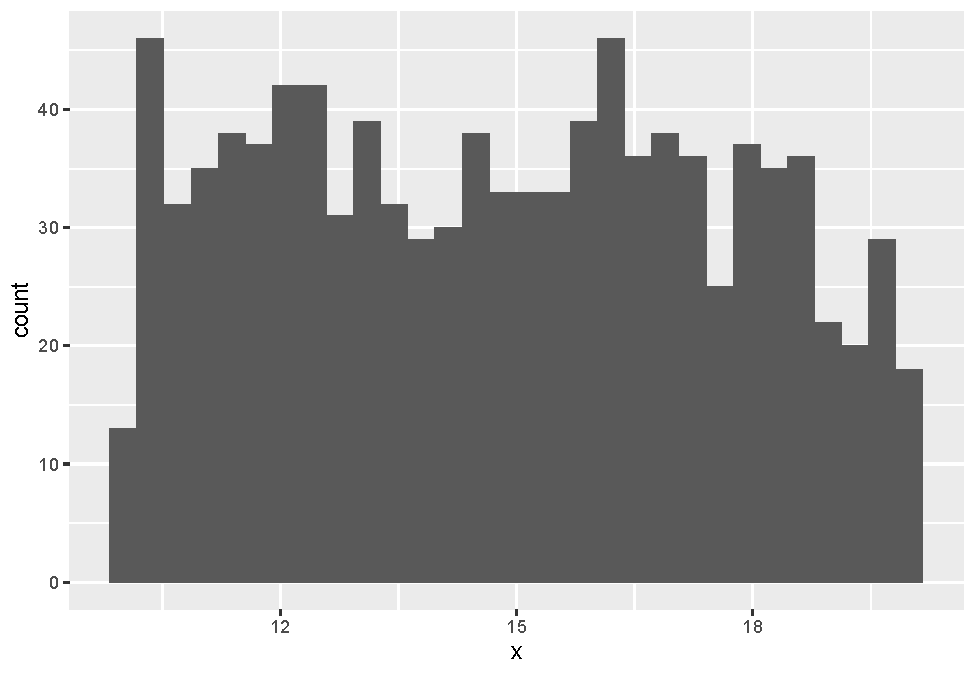
\includegraphics[width=0.75\linewidth]{EnvDataScience_files/figure-latex/statrunif-1} 

}

\caption{Random uniform histogram}\label{fig:statrunif}
\end{figure}

\begin{Shaded}
\begin{Highlighting}[]
\NormalTok{y }\OtherTok{\textless{}{-}} \FunctionTok{as\_tibble}\NormalTok{(}\FunctionTok{rnorm}\NormalTok{(}\AttributeTok{n=}\DecValTok{1000}\NormalTok{, }\AttributeTok{mean=}\DecValTok{100}\NormalTok{, }\AttributeTok{sd=}\DecValTok{10}\NormalTok{))}
\FunctionTok{names}\NormalTok{(y) }\OtherTok{\textless{}{-}} \StringTok{\textquotesingle{}y\textquotesingle{}}
\FunctionTok{ggplot}\NormalTok{(y, }\FunctionTok{aes}\NormalTok{(}\AttributeTok{x=}\NormalTok{y)) }\SpecialCharTok{+} \FunctionTok{geom\_histogram}\NormalTok{()}
\end{Highlighting}
\end{Shaded}

\begin{figure}

{\centering 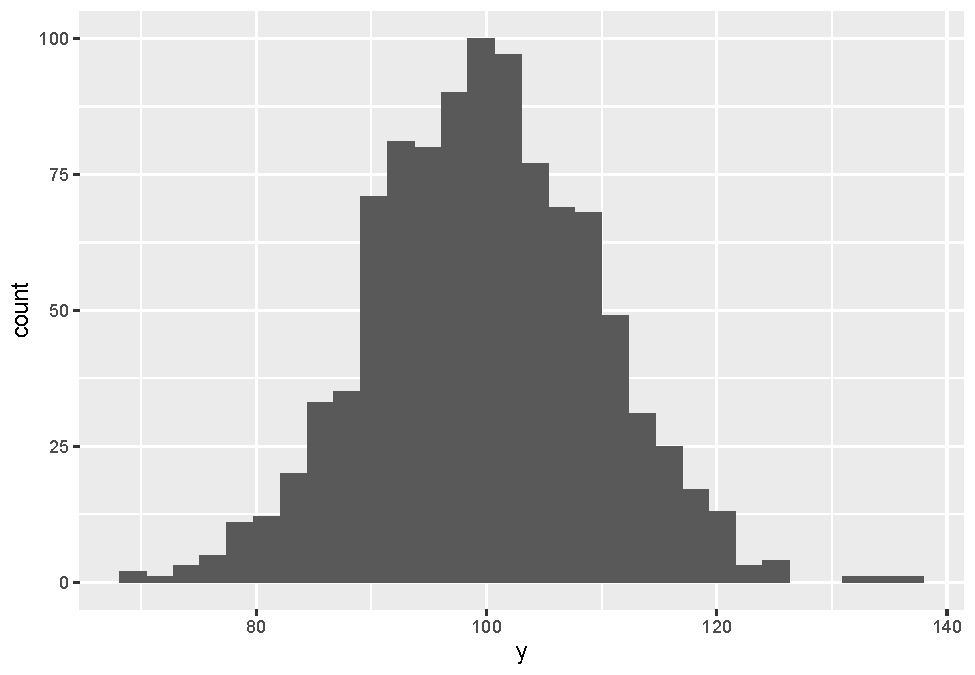
\includegraphics[width=0.75\linewidth]{EnvDataScience_files/figure-latex/statrnorm-1} 

}

\caption{Random normal histogram}\label{fig:statrnorm}
\end{figure}

\begin{Shaded}
\begin{Highlighting}[]
\FunctionTok{ggplot}\NormalTok{(y, }\FunctionTok{aes}\NormalTok{(}\AttributeTok{x=}\NormalTok{y)) }\SpecialCharTok{+} \FunctionTok{geom\_density}\NormalTok{()}
\end{Highlighting}
\end{Shaded}

\begin{figure}

{\centering 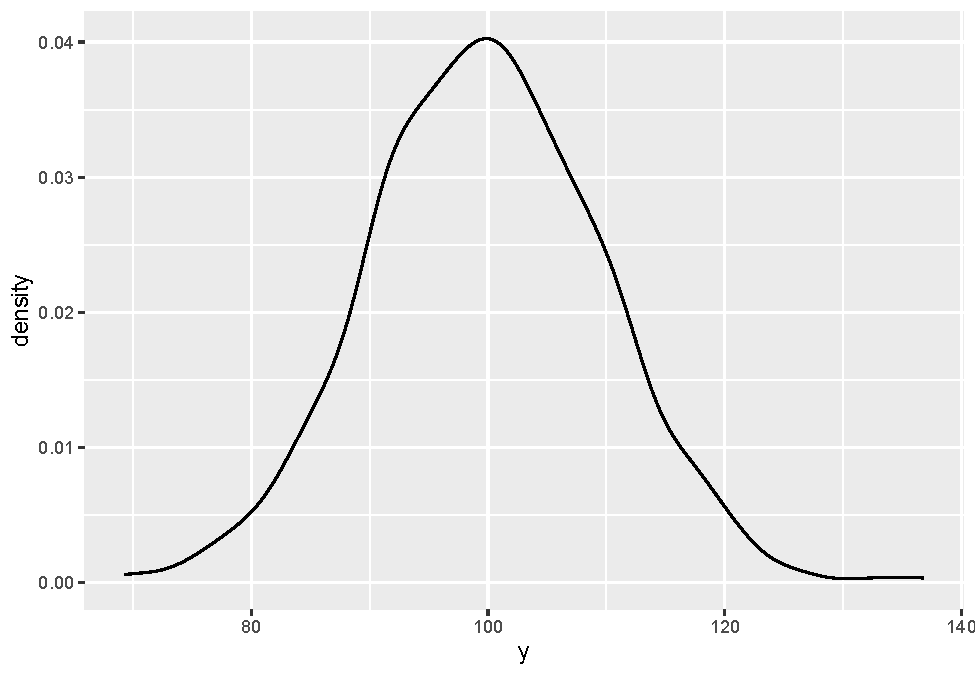
\includegraphics[width=0.75\linewidth]{EnvDataScience_files/figure-latex/statrnormDens-1} 

}

\caption{Random normal density plot}\label{fig:statrnormDens}
\end{figure}

\begin{Shaded}
\begin{Highlighting}[]
\NormalTok{xy }\OtherTok{\textless{}{-}} \FunctionTok{bind\_cols}\NormalTok{(x,y)}
\end{Highlighting}
\end{Shaded}

\begin{Shaded}
\begin{Highlighting}[]
\FunctionTok{ggplot}\NormalTok{(xy, }\FunctionTok{aes}\NormalTok{(}\AttributeTok{x=}\NormalTok{x,}\AttributeTok{y=}\NormalTok{y)) }\SpecialCharTok{+} \FunctionTok{geom\_point}\NormalTok{()}
\end{Highlighting}
\end{Shaded}

\begin{figure}

{\centering 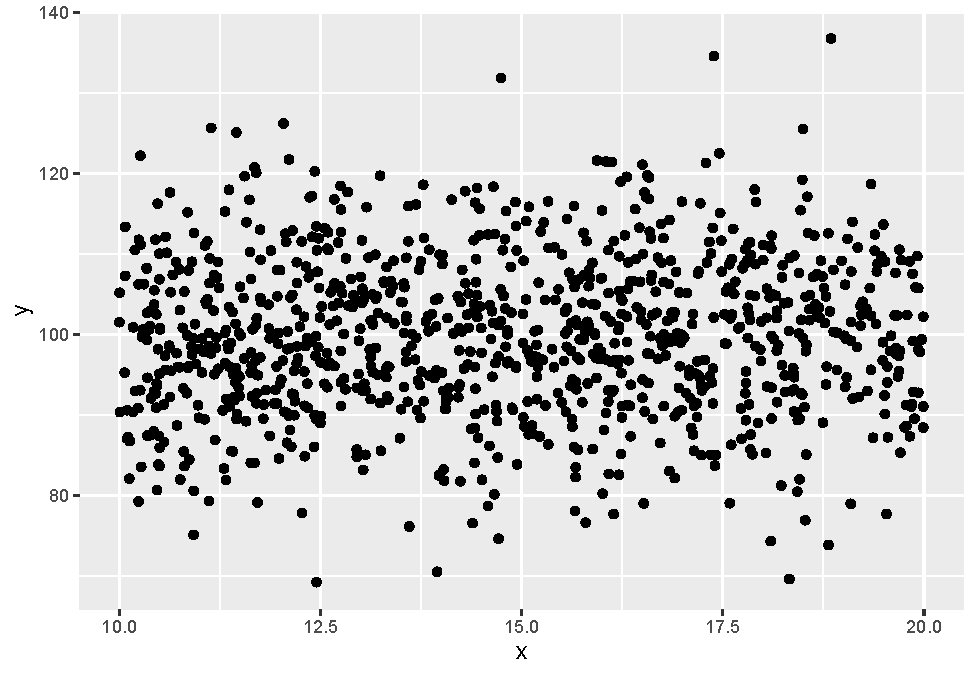
\includegraphics[width=0.75\linewidth]{EnvDataScience_files/figure-latex/statrnomrunif-1} 

}

\caption{Random normal plotted against random uniform}\label{fig:statrnomrunif}
\end{figure}

\section{\texorpdfstring{Correlation r and Coefficient of Determination r\textsuperscript{2}}{Correlation r and Coefficient of Determination r2}}\label{correlation}

\index{correlation}In the visualization chapter, we looked at creating scatter plots and also arrays of scatter plots where we could compare variables to visually see if they might be positively or negatively correlated. A statistic that is commonly used for this is the \emph{Pearson product-moment correlation coefficient} or r statistic.

We'll look at the formula for r below, but it's easier to just use the \texttt{cor} function. You just need the two variables as vector inputs in R to return the r statistic. Squaring r to r\textsuperscript{2} is the \emph{coefficient of determination} \index{coefficient of determination}\index{r squared}and can be interpreted as the amount of the variation in the dependent variable y that that is ``explained'' by variation in the independent variable x. This coefficient will always be positive, with a maximum of 1 or 100\%.

If we create two random variables, uniform or normal, there shouldn't be any correlation. We'll do this five times each set:

\begin{Shaded}
\begin{Highlighting}[]
\ControlFlowTok{for}\NormalTok{ (i }\ControlFlowTok{in} \DecValTok{1}\SpecialCharTok{:}\DecValTok{5}\NormalTok{) \{}\FunctionTok{print}\NormalTok{(}\FunctionTok{paste}\NormalTok{(i, }\FunctionTok{cor}\NormalTok{(}\FunctionTok{rnorm}\NormalTok{(}\DecValTok{100}\NormalTok{), }\FunctionTok{rnorm}\NormalTok{(}\DecValTok{100}\NormalTok{))))\}}
\end{Highlighting}
\end{Shaded}

\begin{verbatim}
## [1] "1 -0.306867610791146"
## [1] "2 0.0435334582689279"
## [1] "3 0.0218834471816236"
## [1] "4 -0.0505322386278771"
## [1] "5 -0.0100788763936654"
\end{verbatim}

\begin{Shaded}
\begin{Highlighting}[]
\ControlFlowTok{for}\NormalTok{ (i }\ControlFlowTok{in} \DecValTok{1}\SpecialCharTok{:}\DecValTok{5}\NormalTok{) \{}\FunctionTok{print}\NormalTok{(}\FunctionTok{paste}\NormalTok{(i, }\FunctionTok{cor}\NormalTok{(}\FunctionTok{runif}\NormalTok{(}\DecValTok{100}\NormalTok{), }\FunctionTok{runif}\NormalTok{(}\DecValTok{100}\NormalTok{))))\}}
\end{Highlighting}
\end{Shaded}

\begin{verbatim}
## [1] "1 -0.000369334235807692"
## [1] "2 0.0104243143064686"
## [1] "3 0.0100473186730334"
## [1] "4 -0.0206269090624089"
## [1] "5 0.158031281575223"
\end{verbatim}

\begin{Shaded}
\begin{Highlighting}[]
\ControlFlowTok{for}\NormalTok{ (i }\ControlFlowTok{in} \DecValTok{1}\SpecialCharTok{:}\DecValTok{5}\NormalTok{) \{}\FunctionTok{print}\NormalTok{(}\FunctionTok{paste}\NormalTok{(i, }\FunctionTok{cor}\NormalTok{(}\FunctionTok{rnorm}\NormalTok{(}\DecValTok{100}\NormalTok{), }\FunctionTok{runif}\NormalTok{(}\DecValTok{100}\NormalTok{))))\}}
\end{Highlighting}
\end{Shaded}

\begin{verbatim}
## [1] "1 0.0594965540459601"
## [1] "2 0.0308884565713835"
## [1] "3 0.0666190005779386"
## [1] "4 -0.113543452263837"
## [1] "5 -0.0126068334715897"
\end{verbatim}

But variables such as temperature and elevation in the Sierra will be strongly negatively correlated, as seen in the scatter plot and the r value close to -1, and have a high r\textsuperscript{2} (Figure \ref{fig:statNegScatter}).

\begin{Shaded}
\begin{Highlighting}[]
\FunctionTok{library}\NormalTok{(igisci); }\FunctionTok{library}\NormalTok{(tidyverse)}
\NormalTok{sierra }\OtherTok{\textless{}{-}}\NormalTok{ sierraFeb }\SpecialCharTok{\%\textgreater{}\%} \FunctionTok{filter}\NormalTok{(}\SpecialCharTok{!}\FunctionTok{is.na}\NormalTok{(TEMPERATURE))}
\NormalTok{elev }\OtherTok{\textless{}{-}}\NormalTok{ sierra}\SpecialCharTok{$}\NormalTok{ELEVATION; tC }\OtherTok{\textless{}{-}}\NormalTok{ sierra}\SpecialCharTok{$}\NormalTok{TEMPERATURE}
\FunctionTok{plot}\NormalTok{(elev, tC)}
\end{Highlighting}
\end{Shaded}

\begin{figure}

{\centering 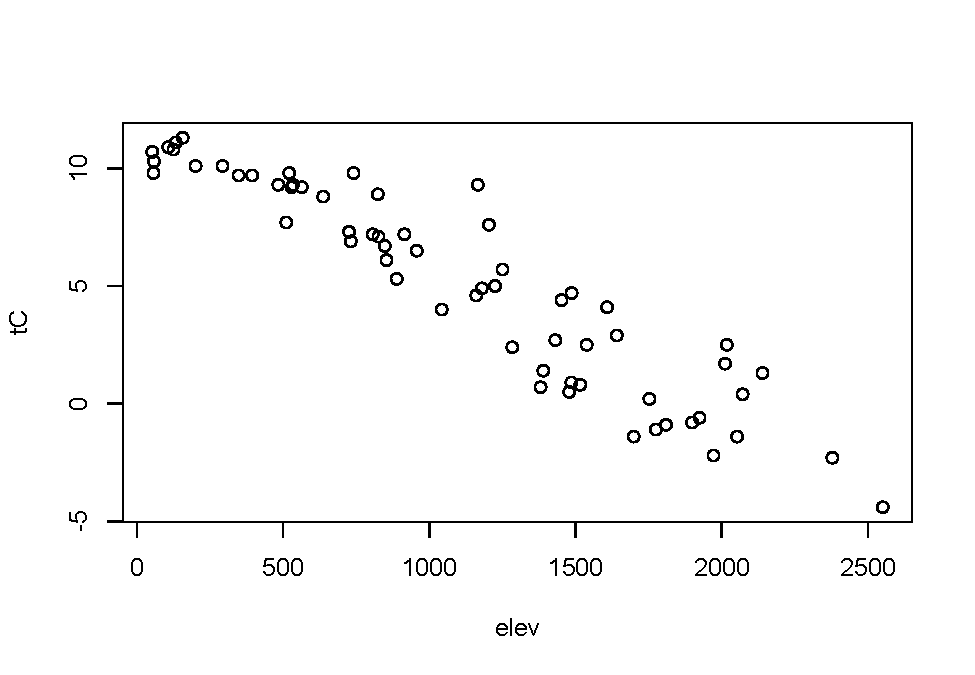
\includegraphics[width=0.75\linewidth]{EnvDataScience_files/figure-latex/statNegScatter-1} 

}

\caption{Scatter plot illustrating negative correlation}\label{fig:statNegScatter}
\end{figure}

\begin{Shaded}
\begin{Highlighting}[]
\FunctionTok{cor}\NormalTok{(elev, tC)}
\end{Highlighting}
\end{Shaded}

\begin{verbatim}
## [1] -0.9357801
\end{verbatim}

\begin{Shaded}
\begin{Highlighting}[]
\FunctionTok{cor}\NormalTok{(elev, tC)}\SpecialCharTok{\^{}}\DecValTok{2}
\end{Highlighting}
\end{Shaded}

\begin{verbatim}
## [1] 0.8756845
\end{verbatim}

\index{cor}While you don't need to use this, since the \texttt{cor} function is easier to type, it's interesting to know that the formula for Pearson's correlation coefficient is something that you can actually code in R, taking advantage of its vectorization methods:

\[
r = \frac{\sum{(x_i-\overline{x})(y_i-\overline{y})}}{\sqrt{\sum{(x_i-\overline{x})^2\sum(y_i-\overline{y})^2}}}
\]

\begin{Shaded}
\begin{Highlighting}[]
\NormalTok{r }\OtherTok{\textless{}{-}} \FunctionTok{sum}\NormalTok{((elev}\SpecialCharTok{{-}}\FunctionTok{mean}\NormalTok{(elev))}\SpecialCharTok{*}\NormalTok{(tC}\SpecialCharTok{{-}}\FunctionTok{mean}\NormalTok{(tC)))}\SpecialCharTok{/}
     \FunctionTok{sqrt}\NormalTok{(}\FunctionTok{sum}\NormalTok{((elev}\SpecialCharTok{{-}}\FunctionTok{mean}\NormalTok{(elev))}\SpecialCharTok{\^{}}\DecValTok{2}\SpecialCharTok{*}\FunctionTok{sum}\NormalTok{((tC}\SpecialCharTok{{-}}\FunctionTok{mean}\NormalTok{(tC))}\SpecialCharTok{\^{}}\DecValTok{2}\NormalTok{)))}
\NormalTok{r}
\end{Highlighting}
\end{Shaded}

\begin{verbatim}
## [1] -0.9357801
\end{verbatim}

\begin{Shaded}
\begin{Highlighting}[]
\NormalTok{r}\SpecialCharTok{\^{}}\DecValTok{2}
\end{Highlighting}
\end{Shaded}

\begin{verbatim}
## [1] 0.8756845
\end{verbatim}

Another version of the formula runs faster, so might be what R uses, but you'll never notice the time difference:

\[
r = \frac{n(\sum{xy})-(\sum{x})(\sum{y})}{\sqrt{(n\sum{x^2}-(\sum{x})^2)(n\sum{y^2}-(\sum{y})^2)}}
\]

\begin{Shaded}
\begin{Highlighting}[]
\NormalTok{n }\OtherTok{\textless{}{-}} \FunctionTok{length}\NormalTok{(elev)}
\NormalTok{r }\OtherTok{\textless{}{-}}\NormalTok{ (n}\SpecialCharTok{*}\FunctionTok{sum}\NormalTok{(elev}\SpecialCharTok{*}\NormalTok{tC)}\SpecialCharTok{{-}}\FunctionTok{sum}\NormalTok{(elev)}\SpecialCharTok{*}\FunctionTok{sum}\NormalTok{(tC))}\SpecialCharTok{/}
  \FunctionTok{sqrt}\NormalTok{((n}\SpecialCharTok{*}\FunctionTok{sum}\NormalTok{(elev}\SpecialCharTok{\^{}}\DecValTok{2}\NormalTok{)}\SpecialCharTok{{-}}\FunctionTok{sum}\NormalTok{(elev)}\SpecialCharTok{\^{}}\DecValTok{2}\NormalTok{)}\SpecialCharTok{*}\NormalTok{(n}\SpecialCharTok{*}\FunctionTok{sum}\NormalTok{(tC}\SpecialCharTok{\^{}}\DecValTok{2}\NormalTok{)}\SpecialCharTok{{-}}\FunctionTok{sum}\NormalTok{(tC)}\SpecialCharTok{\^{}}\DecValTok{2}\NormalTok{))}
\NormalTok{r}
\end{Highlighting}
\end{Shaded}

\begin{verbatim}
## [1] -0.9357801
\end{verbatim}

\begin{Shaded}
\begin{Highlighting}[]
\NormalTok{r}\SpecialCharTok{\^{}}\DecValTok{2}
\end{Highlighting}
\end{Shaded}

\begin{verbatim}
## [1] 0.8756845
\end{verbatim}

\ldots{} and as you can see, all three methods give the same results.

\subsection{Displaying correlation in a pairs plot}\label{displaying-correlation-in-a-pairs-plot}

\index{pairs plot}We can use another type of pairs plot from the \textbf{psych} package to look at the correlation coefficient in the upper-right part of the pairs plot, since correlation can be determined between x and y or y and x; the result is the same. In contrast to what we'll see in regression models, there doesn't have to be one \emph{explanatory} (or independent) variable and one \emph{response} (or dependent) variable; either one will do. The r value shows both the direction (positive or negative) and the magnitude of the correlation, with values closer to 1 or -1 being more correlated (Figure \ref{fig:statPairs}).

\begin{Shaded}
\begin{Highlighting}[]
\FunctionTok{library}\NormalTok{(psych)}
\NormalTok{sierraFeb }\SpecialCharTok{\%\textgreater{}\%}
\NormalTok{     dplyr}\SpecialCharTok{::}\FunctionTok{select}\NormalTok{(ELEVATION}\SpecialCharTok{:}\NormalTok{TEMPERATURE) }\SpecialCharTok{\%\textgreater{}\%}
     \FunctionTok{pairs.panels}\NormalTok{(}\AttributeTok{method =} \StringTok{"pearson"}\NormalTok{, }\CommentTok{\# correlation method}
             \AttributeTok{hist.col =} \StringTok{"\#00AFBB"}\NormalTok{,}
             \AttributeTok{density =} \ConstantTok{TRUE}\NormalTok{, }\CommentTok{\# show density plots}
             \AttributeTok{ellipses =}\NormalTok{ F, }\AttributeTok{smooth =}\NormalTok{ F) }\CommentTok{\# unneeded  }
\end{Highlighting}
\end{Shaded}

\begin{figure}

{\centering 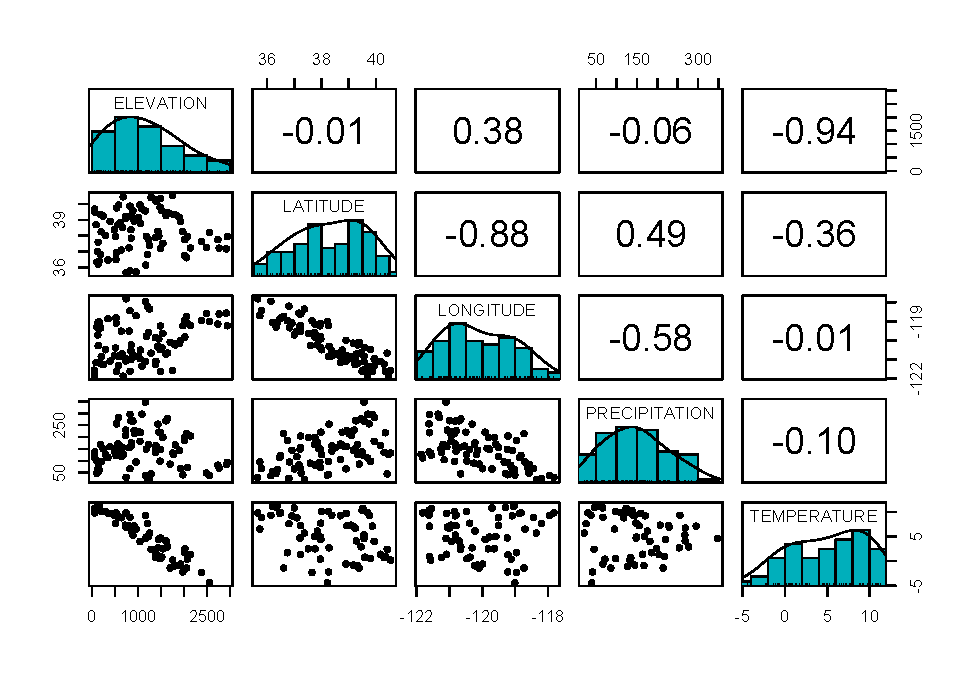
\includegraphics[width=0.75\linewidth]{EnvDataScience_files/figure-latex/statPairs-1} 

}

\caption{Pairs plot with r values}\label{fig:statPairs}
\end{figure}

We can clearly see in the graphs the negative relationships between elevation and temperature and between latitude and longitude (what is that telling us?), and these correspond to strongly negative correlation coefficients.

\textbf{One problem with Pearson}: While there's nothing wrong with the correlation coefficient, Pearson's name, along with some other pioneers of statistics like Fisher, is tainted by an association with the racist field of \emph{eugenics}. But the mathematics is not to blame, and the correlation coefficient is still as useful as ever. Maybe we can just say that Pearson \emph{discovered} the correlation coefficient\ldots{}

\section{Statistical Tests}\label{statistical-tests}

Tests that compare our data to other data or look at relationships among variables are important statistical methods, and you should refer to statistical references to best understand how to apply the appropriate methods for your research.

\subsection{Comparing samples and groupings with a t test and a non-parametric Kruskal-Wallis Rank Sum test}\label{comparing-samples-and-groupings-with-a-t-test-and-a-non-parametric-kruskal-wallis-rank-sum-test}

\index{t test}\index{Kruskal-Wallis Rank Sum Test}\index{non-parametric test}A common need in environmental research is to compare samples of a phenomenon (e.g.~Figure \ref{fig:statNDVIpheno}) or compare samples with an assumed standard population. The simplest application of this is the t-test, which can only involve comparing two samples or one sample with a population. After this, we'll look at analysis of variance, extending this to allow for more than two groups. Start by building \texttt{XSptsPheno} from code in the Histogram section (\ref{histogram}) of the Visualization chapter, then proceed:

\begin{Shaded}
\begin{Highlighting}[]
\NormalTok{XSptsPheno }\SpecialCharTok{\%\textgreater{}\%}
  \FunctionTok{ggplot}\NormalTok{(}\FunctionTok{aes}\NormalTok{(NDVI, }\AttributeTok{fill=}\NormalTok{phenology)) }\SpecialCharTok{+}
  \FunctionTok{geom\_density}\NormalTok{(}\AttributeTok{alpha=}\FloatTok{0.2}\NormalTok{)}
\end{Highlighting}
\end{Shaded}

\begin{figure}

{\centering 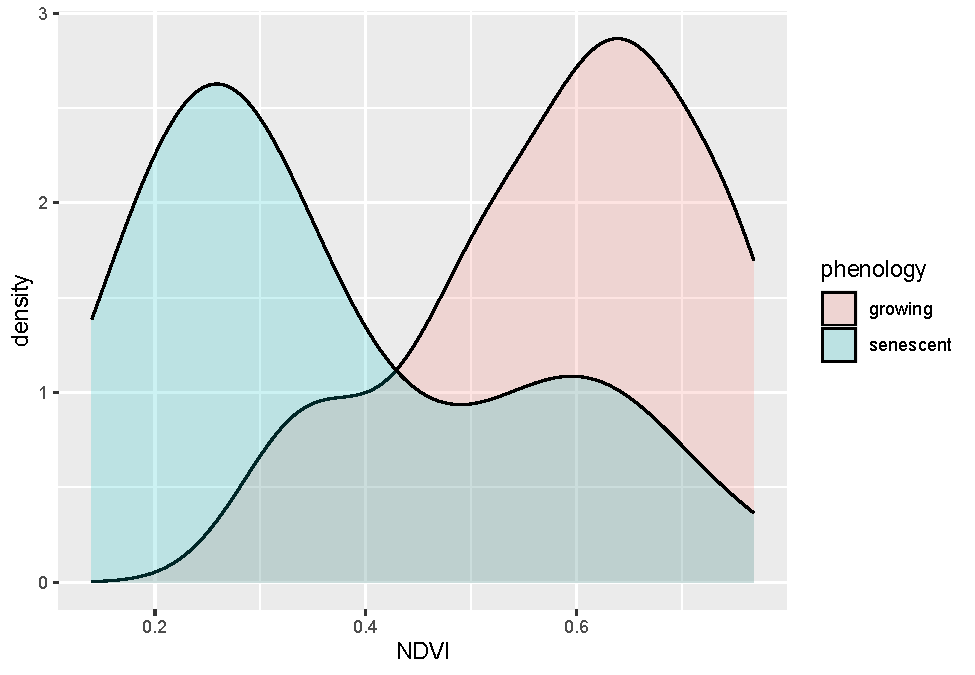
\includegraphics[width=0.75\linewidth]{EnvDataScience_files/figure-latex/statNDVIpheno-1} 

}

\caption{NDVI by phenology}\label{fig:statNDVIpheno}
\end{figure}

\begin{Shaded}
\begin{Highlighting}[]
\FunctionTok{t.test}\NormalTok{(NDVI}\SpecialCharTok{\textasciitilde{}}\NormalTok{phenology, }\AttributeTok{data=}\NormalTok{XSptsPheno) }
\end{Highlighting}
\end{Shaded}

\footnotesize

\begin{verbatim}
## 
##  Welch Two Sample t-test
## 
## data:  NDVI by phenology
## t = 5.4952, df = 52.03, p-value = 1.19e-06
## alternative hypothesis: true difference in means between group growing and group senescent is not equal to 0
## 95 percent confidence interval:
##  0.1421785 0.3057412
## sample estimates:
##   mean in group growing mean in group senescent 
##               0.5901186               0.3661588
\end{verbatim}

\normalsize

One condition for using a t test is that our data is \index{normally distributed}normally distributed. While these data sets \emph{appear} reasonably normal, though with a bit of bimodality especially for the senescent group, the \index{Shapiro-Wilk test for normality}Shapiro-Wilk test (which uses a null hypothesis of normal) has a p value \textless{} 0.05 for the senescent group, so the data can't be assumed to be normal.

\begin{Shaded}
\begin{Highlighting}[]
\FunctionTok{shapiro.test}\NormalTok{(XSptsPheno}\SpecialCharTok{$}\NormalTok{NDVI[XSptsPheno}\SpecialCharTok{$}\NormalTok{phenology}\SpecialCharTok{==}\StringTok{"growing"}\NormalTok{])}
\end{Highlighting}
\end{Shaded}

\begin{verbatim}
## 
##  Shapiro-Wilk normality test
## 
## data:  XSptsPheno$NDVI[XSptsPheno$phenology == "growing"]
## W = 0.93608, p-value = 0.07918
\end{verbatim}

\begin{Shaded}
\begin{Highlighting}[]
\FunctionTok{shapiro.test}\NormalTok{(XSptsPheno}\SpecialCharTok{$}\NormalTok{NDVI[XSptsPheno}\SpecialCharTok{$}\NormalTok{phenology}\SpecialCharTok{==}\StringTok{"senescent"}\NormalTok{])}
\end{Highlighting}
\end{Shaded}

\begin{verbatim}
## 
##  Shapiro-Wilk normality test
## 
## data:  XSptsPheno$NDVI[XSptsPheno$phenology == "senescent"]
## W = 0.88728, p-value = 0.004925
\end{verbatim}

Therefore we should use a non-parametric alternative such as the
Kruskal-Wallis Rank Sum test:

\begin{Shaded}
\begin{Highlighting}[]
\FunctionTok{kruskal.test}\NormalTok{(NDVI}\SpecialCharTok{\textasciitilde{}}\NormalTok{phenology, }\AttributeTok{data=}\NormalTok{XSptsPheno)}
\end{Highlighting}
\end{Shaded}

\footnotesize

\begin{verbatim}
## 
##  Kruskal-Wallis rank sum test
## 
## data:  NDVI by phenology
## Kruskal-Wallis chi-squared = 19.164, df = 1, p-value = 1.199e-05
\end{verbatim}

\normalsize

\textbf{A bit of a review on significance tests and p values}

\index{significance tests}\index{p or Pr values}First, each type of test will be testing a particular summary statistic, like the t test is comparing means and the analysis of variance will be comparing variances. In confirmatory statistical tests, you're always seeing if you can reject the null hypothesis that there's no difference, so in the t test or the rank sum test above that compares two samples, it's that there's no difference between two samples.

There will of course nearly always be some difference, so you might think that you'd always reject the \index{null hypothesis}null hypothesis that there's no difference. That's where random error and probability comes in. You can accept a certain amount of error -- say 5\% -- to be able to say that the difference in values could have occurred by chance. That 5\% or 0.05 is often called the ``significance level'' and is the probability of the two values being the same that you're willing to accept. (The remainder 0.95 is often called the confidence level, the extent to which you're confident that rejecting the null hypothesis and accepting the working hypothesis is correct.)

When R reports the p (or Pr) probability value, you compare that value to that significance level to see if it's lower, and then use that to possibly reject the null hypothesis and accept the working hypothesis. R will simply report the p value and commonly show asterisks along with it to indicate if it's lower than various common significance levels, like 0.1, 0.05, 0.01, and 0.001.

\subsubsection{Runoff and Sediment Yield under Eucalyptus vs Oaks -- is there a difference?}\label{runoff-and-sediment-yield-under-eucalyptus-vs-oaks-is-there-a-difference}

Starting with the Data Abstraction chapter, one of the data sets we've been looking at is from a study of \index{runoff analysis}runoff and sediment yield\index{sediment yield analysis} under paired eucalyptus and coast live oak sites, and we might want to analyze this data statistically to consider some basic research questions. These are discussed at greater length in Thompson et al. (\citeproc{ref-eucoak}{2016}), but the key questions are:

\begin{itemize}
\tightlist
\item
  \emph{Is the runoff under eucalyptus canopy significantly different from that under oaks?}
\item
  \emph{Is the sediment yield under eucalyptus canopy significantly different from that under oaks?}
\end{itemize}

We'll start with the first, since this was the focus on the first part of the study where multiple variables that influence runoff were measured, such as soil hydrophobicity resulting from the chemical effects of eucalyptus, and any rainfall contrasts at each site and between sites. For runoff, we'll then start by test for normality of each of the two samples (euc and oak) which shows clearly that both samples are non-normal.

\begin{Shaded}
\begin{Highlighting}[]
\FunctionTok{shapiro.test}\NormalTok{(tidy\_eucoak}\SpecialCharTok{$}\NormalTok{runoff\_L[tidy\_eucoak}\SpecialCharTok{$}\NormalTok{tree }\SpecialCharTok{==} \StringTok{"euc"}\NormalTok{])}
\end{Highlighting}
\end{Shaded}

\begin{verbatim}
## 
##  Shapiro-Wilk normality test
## 
## data:  tidy_eucoak$runoff_L[tidy_eucoak$tree == "euc"]
## W = 0.74241, p-value = 4.724e-11
\end{verbatim}

\begin{Shaded}
\begin{Highlighting}[]
\FunctionTok{shapiro.test}\NormalTok{(tidy\_eucoak}\SpecialCharTok{$}\NormalTok{runoff\_L[tidy\_eucoak}\SpecialCharTok{$}\NormalTok{tree }\SpecialCharTok{==} \StringTok{"oak"}\NormalTok{])}
\end{Highlighting}
\end{Shaded}

\begin{verbatim}
## 
##  Shapiro-Wilk normality test
## 
## data:  tidy_eucoak$runoff_L[tidy_eucoak$tree == "oak"]
## W = 0.71744, p-value = 1.698e-11
\end{verbatim}

So we might apply the non-parametric Kruskal-Wallis test \ldots{}

\begin{Shaded}
\begin{Highlighting}[]
\FunctionTok{kruskal.test}\NormalTok{(runoff\_L}\SpecialCharTok{\textasciitilde{}}\NormalTok{tree, }\AttributeTok{data=}\NormalTok{tidy\_eucoak)}
\end{Highlighting}
\end{Shaded}

\begin{verbatim}
## 
##  Kruskal-Wallis rank sum test
## 
## data:  runoff_L by tree
## Kruskal-Wallis chi-squared = 2.2991, df = 1, p-value = 0.1294
\end{verbatim}

\ldots{} and no significant difference can be seen. If we look at the data graphically, this makes sense, since the distributions are not dissimilar (Figure \ref{fig:statEucOakRunoff}).

\begin{Shaded}
\begin{Highlighting}[]
\NormalTok{tidy\_eucoak }\SpecialCharTok{\%\textgreater{}\%}
  \FunctionTok{ggplot}\NormalTok{(}\FunctionTok{aes}\NormalTok{(}\FunctionTok{log}\NormalTok{(runoff\_L),}\AttributeTok{fill=}\NormalTok{tree)) }\SpecialCharTok{+}
  \FunctionTok{geom\_density}\NormalTok{(}\AttributeTok{alpha=}\FloatTok{0.2}\NormalTok{)}
\end{Highlighting}
\end{Shaded}

\begin{figure}

{\centering 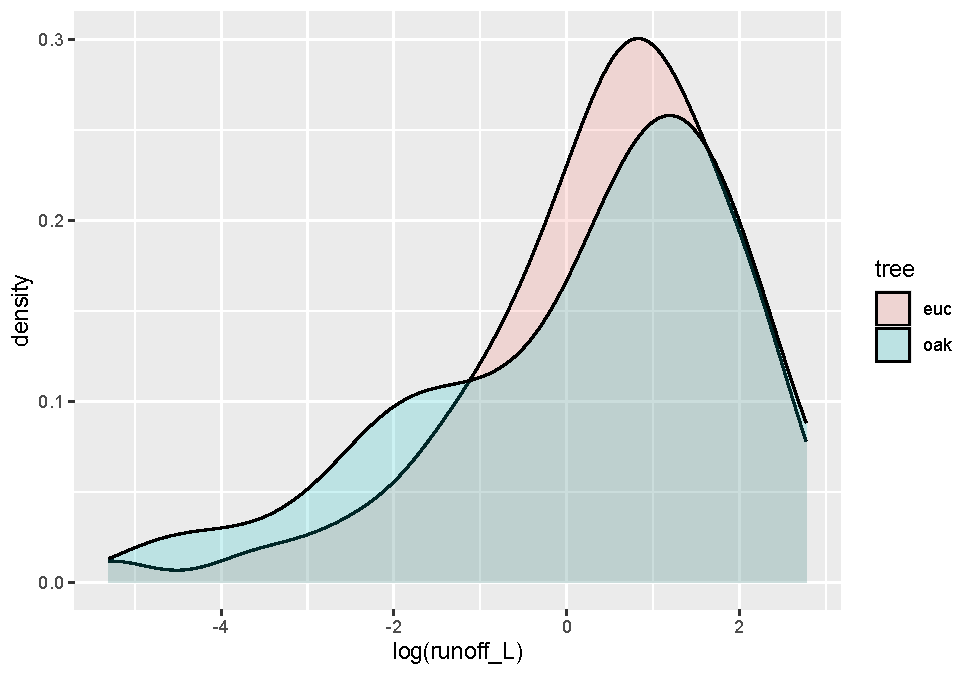
\includegraphics[width=0.75\linewidth]{EnvDataScience_files/figure-latex/statEucOakRunoff-1} 

}

\caption{Runoff under eucalyptus and oak in Bay Area sites}\label{fig:statEucOakRunoff}
\end{figure}

However, some of this may result from major variations among sites, which is apparent in a site-grouped boxplot (Figure \ref{fig:statSiteGrouped}).

\begin{Shaded}
\begin{Highlighting}[]
\FunctionTok{ggplot}\NormalTok{(}\AttributeTok{data =}\NormalTok{ tidy\_eucoak) }\SpecialCharTok{+}
  \FunctionTok{geom\_boxplot}\NormalTok{(}\FunctionTok{aes}\NormalTok{(}\AttributeTok{x=}\NormalTok{site, }\AttributeTok{y=}\NormalTok{runoff\_L, }\AttributeTok{color=}\NormalTok{tree))}
\end{Highlighting}
\end{Shaded}

\begin{figure}

{\centering 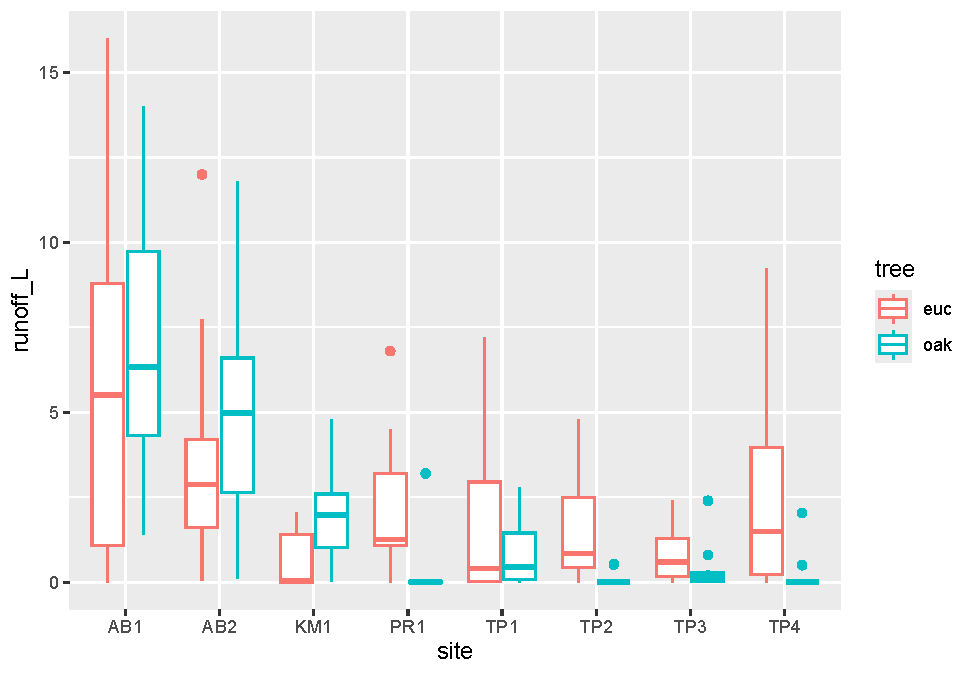
\includegraphics[width=0.75\linewidth]{EnvDataScience_files/figure-latex/statSiteGrouped-1} 

}

\caption{Runoff at various sites contrasting euc and oak}\label{fig:statSiteGrouped}
\end{figure}

We might restrict our analysis to Tilden Park sites in the East Bay, where there's more of a difference (Figure \ref{fig:statTildenSites}), but the sample size is very small.

\begin{Shaded}
\begin{Highlighting}[]
\NormalTok{tilden }\OtherTok{\textless{}{-}}\NormalTok{ tidy\_eucoak }\SpecialCharTok{\%\textgreater{}\%} \FunctionTok{filter}\NormalTok{(}\FunctionTok{str\_detect}\NormalTok{(tidy\_eucoak}\SpecialCharTok{$}\NormalTok{site,}\StringTok{"TP"}\NormalTok{))}
\NormalTok{tilden }\SpecialCharTok{\%\textgreater{}\%}
  \FunctionTok{ggplot}\NormalTok{(}\FunctionTok{aes}\NormalTok{(}\FunctionTok{log}\NormalTok{(runoff\_L),}\AttributeTok{fill=}\NormalTok{tree)) }\SpecialCharTok{+}
  \FunctionTok{geom\_density}\NormalTok{(}\AttributeTok{alpha=}\FloatTok{0.2}\NormalTok{)}
\end{Highlighting}
\end{Shaded}

\begin{figure}

{\centering 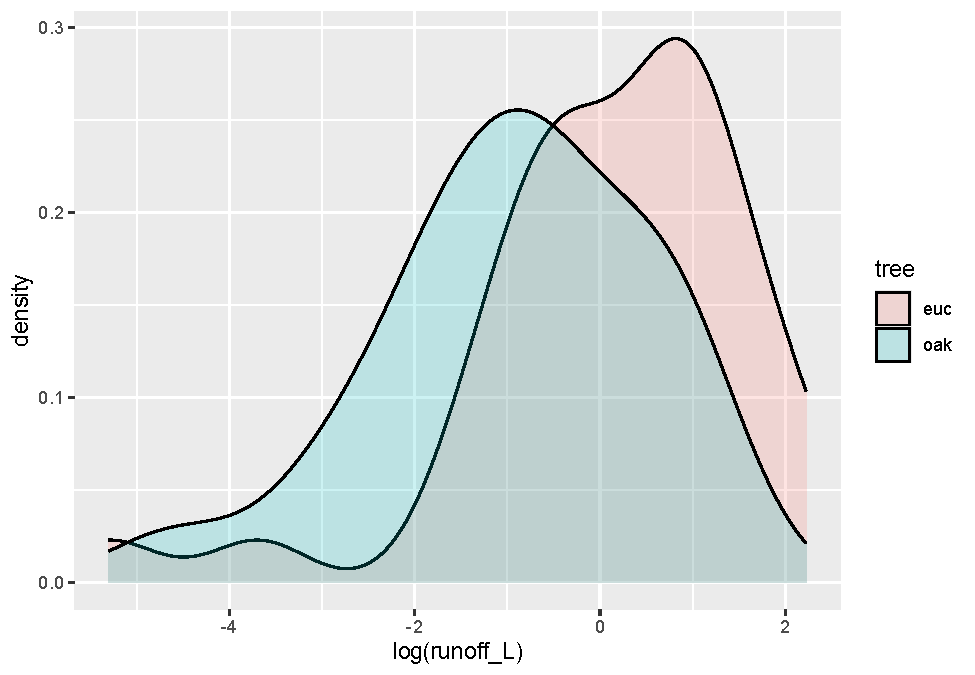
\includegraphics[width=0.75\linewidth]{EnvDataScience_files/figure-latex/statTildenSites-1} 

}

\caption{East Bay sites}\label{fig:statTildenSites}
\end{figure}

\begin{Shaded}
\begin{Highlighting}[]
\FunctionTok{shapiro.test}\NormalTok{(tilden}\SpecialCharTok{$}\NormalTok{runoff\_L[tilden}\SpecialCharTok{$}\NormalTok{tree }\SpecialCharTok{==} \StringTok{"euc"}\NormalTok{])}
\end{Highlighting}
\end{Shaded}

\begin{verbatim}
## 
##  Shapiro-Wilk normality test
## 
## data:  tilden$runoff_L[tilden$tree == "euc"]
## W = 0.73933, p-value = 1.764e-07
\end{verbatim}

\begin{Shaded}
\begin{Highlighting}[]
\FunctionTok{shapiro.test}\NormalTok{(tilden}\SpecialCharTok{$}\NormalTok{runoff\_L[tilden}\SpecialCharTok{$}\NormalTok{tree }\SpecialCharTok{==} \StringTok{"oak"}\NormalTok{])}
\end{Highlighting}
\end{Shaded}

\begin{verbatim}
## 
##  Shapiro-Wilk normality test
## 
## data:  tilden$runoff_L[tilden$tree == "oak"]
## W = 0.59535, p-value = 8.529e-10
\end{verbatim}

So once again, as is common with small sample sets, we need a non-parametric test.

\begin{Shaded}
\begin{Highlighting}[]
\FunctionTok{kruskal.test}\NormalTok{(runoff\_L}\SpecialCharTok{\textasciitilde{}}\NormalTok{tree, }\AttributeTok{data=}\NormalTok{tilden)}
\end{Highlighting}
\end{Shaded}

\begin{verbatim}
## 
##  Kruskal-Wallis rank sum test
## 
## data:  runoff_L by tree
## Kruskal-Wallis chi-squared = 14.527, df = 1, p-value = 0.0001382
\end{verbatim}

\textbf{Sediment Yield}

In the year runoff was studied, there were no runoff events sufficient to mobilize sediments. The next year, January had a big event, so we collected sediments and processed them in the lab.

From the basic sediment yield question listed above we can consider two variants:

\begin{itemize}
\tightlist
\item
  Is there a difference between eucs and oaks in terms of fine sediment yield?
\item
  Is there a difference between eucs and oaks in terms of total sediment yield? (includes litter)
\end{itemize}

So here, we will need to extract fine and total sediment yield from the data and derive group statistics by site (Figure \ref{fig:statEucOakSediment}). As usual, we'll use a faceted density plot to visualize the distributions (Figure \ref{fig:statEucOakFacetSediment}). Then we'll run the test.

\begin{Shaded}
\begin{Highlighting}[]
\NormalTok{eucoaksed }\OtherTok{\textless{}{-}} \FunctionTok{read\_csv}\NormalTok{(}\FunctionTok{ex}\NormalTok{(}\StringTok{"eucoak/eucoaksediment.csv"}\NormalTok{))}
\FunctionTok{summary}\NormalTok{(eucoaksed)}
\end{Highlighting}
\end{Shaded}

\begin{verbatim}
##          id            site          trtype       slope        bulkDensity   
##  Length   :14   Length   :14   Length   :14   Min.   : 9.00   Min.   :0.960  
##  N.unique :14   N.unique : 7   N.unique : 2   1st Qu.:12.00   1st Qu.:1.060  
##  N.blank  : 0   N.blank  : 0   N.blank  : 0   Median :21.00   Median :1.125  
##  Min.nchar: 5   Min.nchar: 3   Min.nchar: 3   Mean   :20.04   Mean   :1.156  
##  Max.nchar: 5   Max.nchar: 3   Max.nchar: 3   3rd Qu.:25.00   3rd Qu.:1.245  
##                                               Max.   :32.00   Max.   :1.490  
##                                                                              
##      litter         Jan08rain     mean_runoff_ratio med_runoff_ratio 
##  Min.   : 25.00   Min.   :228.1   Min.   :0.00450   Min.   :0.00000  
##  1st Qu.: 51.25   1st Qu.:290.8   1st Qu.:0.02285   1st Qu.:0.01105  
##  Median : 77.00   Median :301.1   Median :0.04835   Median :0.04950  
##  Mean   : 76.64   Mean   :298.5   Mean   :0.06679   Mean   :0.06179  
##  3rd Qu.: 95.75   3rd Qu.:317.0   3rd Qu.:0.12172   3rd Qu.:0.09492  
##  Max.   :135.00   Max.   :328.5   Max.   :0.16480   Max.   :0.16430  
##                                                                      
##  std_runoff_ratio     fines_g         litter_g        total_g      
##  Min.   :0.01070   Min.   : 7.50   Min.   :14.00   Min.   : 23.50  
##  1st Qu.:0.01642   1st Qu.:13.30   1st Qu.:18.80   1st Qu.: 35.00  
##  Median :0.02740   Median :18.10   Median :40.40   Median : 60.50  
##  Mean   :0.04355   Mean   :27.77   Mean   :41.32   Mean   : 69.12  
##  3rd Qu.:0.05735   3rd Qu.:45.00   3rd Qu.:57.50   3rd Qu.: 95.50  
##  Max.   :0.11480   Max.   :66.70   Max.   :97.80   Max.   :125.90  
##                    NAs    :1       NAs    :1       NAs    :1       
##  fineTotalRatio   fineRainRatio  
##  Min.   :0.1300   Min.   :0.025  
##  1st Qu.:0.2700   1st Qu.:0.044  
##  Median :0.3900   Median :0.064  
##  Mean   :0.3715   Mean   :0.097  
##  3rd Qu.:0.4900   3rd Qu.:0.141  
##  Max.   :0.5500   Max.   :0.293  
##  NAs    :1        NAs    :1
\end{verbatim}

\begin{Shaded}
\begin{Highlighting}[]
\NormalTok{eucoaksed }\SpecialCharTok{\%\textgreater{}\%}
  \FunctionTok{group\_by}\NormalTok{(trtype) }\SpecialCharTok{\%\textgreater{}\%}
  \FunctionTok{summarize}\NormalTok{(}\AttributeTok{meanfines =} \FunctionTok{mean}\NormalTok{(fines\_g, }\AttributeTok{na.rm=}\NormalTok{T), }\AttributeTok{sdfines =} \FunctionTok{sd}\NormalTok{(fines\_g, }\AttributeTok{na.rm=}\NormalTok{T),}
            \AttributeTok{meantotal =} \FunctionTok{mean}\NormalTok{(total\_g, }\AttributeTok{na.rm=}\NormalTok{T), }\AttributeTok{sdtotal =} \FunctionTok{sd}\NormalTok{(total\_g, }\AttributeTok{na.rm=}\NormalTok{T))}
\end{Highlighting}
\end{Shaded}

\begin{verbatim}
## # A tibble: 2 x 5
##   trtype meanfines sdfines meantotal sdtotal
##   <chr>      <dbl>   <dbl>     <dbl>   <dbl>
## 1 euc         14.2    3.50      48.6    35.0
## 2 oak         39.4   20.4       86.7    26.2
\end{verbatim}

\begin{Shaded}
\begin{Highlighting}[]
\NormalTok{eucoakLong }\OtherTok{\textless{}{-}}\NormalTok{ eucoaksed }\SpecialCharTok{\%\textgreater{}\%} 
  \FunctionTok{pivot\_longer}\NormalTok{(}\AttributeTok{col=}\FunctionTok{c}\NormalTok{(fines\_g,litter\_g), }
               \AttributeTok{names\_to =} \StringTok{"sed\_type"}\NormalTok{, }
               \AttributeTok{values\_to =} \StringTok{"sed\_g"}\NormalTok{)}
\NormalTok{eucoakLong }\SpecialCharTok{\%\textgreater{}\%}
  \FunctionTok{ggplot}\NormalTok{(}\FunctionTok{aes}\NormalTok{(trtype, sed\_g, }\AttributeTok{col=}\NormalTok{sed\_type)) }\SpecialCharTok{+} 
  \FunctionTok{geom\_boxplot}\NormalTok{()}
\end{Highlighting}
\end{Shaded}

\begin{figure}

{\centering 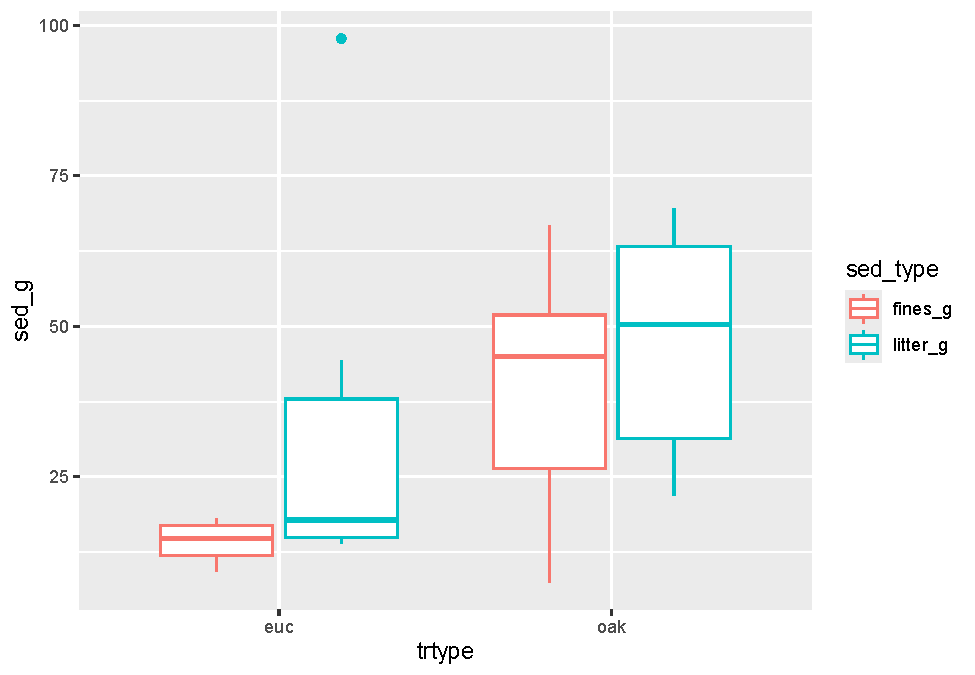
\includegraphics[width=0.75\linewidth]{EnvDataScience_files/figure-latex/statEucOakSediment-1} 

}

\caption{Eucalyptus and oak sediment runoff box plots}\label{fig:statEucOakSediment}
\end{figure}

\begin{Shaded}
\begin{Highlighting}[]
\NormalTok{eucoakLong }\SpecialCharTok{\%\textgreater{}\%}
  \FunctionTok{ggplot}\NormalTok{(}\FunctionTok{aes}\NormalTok{(sed\_g, }\AttributeTok{col=}\NormalTok{sed\_type)) }\SpecialCharTok{+} 
  \FunctionTok{geom\_density}\NormalTok{() }\SpecialCharTok{+}
  \FunctionTok{facet\_grid}\NormalTok{(trtype }\SpecialCharTok{\textasciitilde{}}\NormalTok{ .)}
\end{Highlighting}
\end{Shaded}

\begin{figure}

{\centering 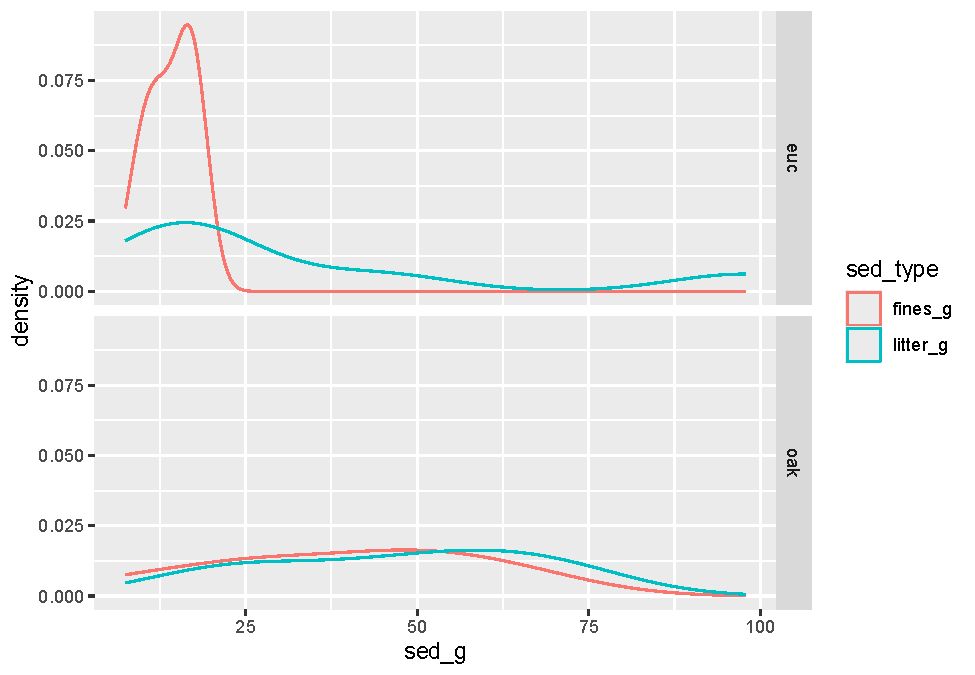
\includegraphics[width=0.75\linewidth]{EnvDataScience_files/figure-latex/statEucOakFacetSediment-1} 

}

\caption{Facet density plot of eucalyptus and oak sediment runoff}\label{fig:statEucOakFacetSediment}
\end{figure}

\textbf{Tests of euc vs oak based on fine sediments:}

\begin{Shaded}
\begin{Highlighting}[]
\FunctionTok{shapiro.test}\NormalTok{(eucoaksed}\SpecialCharTok{$}\NormalTok{fines\_g[eucoaksed}\SpecialCharTok{$}\NormalTok{trtype }\SpecialCharTok{==} \StringTok{"euc"}\NormalTok{])}
\FunctionTok{shapiro.test}\NormalTok{(eucoaksed}\SpecialCharTok{$}\NormalTok{fines\_g[eucoaksed}\SpecialCharTok{$}\NormalTok{trtype }\SpecialCharTok{==} \StringTok{"oak"}\NormalTok{])}
\FunctionTok{t.test}\NormalTok{(fines\_g}\SpecialCharTok{\textasciitilde{}}\NormalTok{trtype, }\AttributeTok{data=}\NormalTok{eucoaksed) }
\end{Highlighting}
\end{Shaded}

\footnotesize

\begin{verbatim}
## 
##  Shapiro-Wilk normality test
## 
## data:  eucoaksed$fines_g[eucoaksed$trtype == "euc"]
## W = 0.9374, p-value = 0.6383
\end{verbatim}

\begin{verbatim}
## 
##  Shapiro-Wilk normality test
## 
## data:  eucoaksed$fines_g[eucoaksed$trtype == "oak"]
## W = 0.96659, p-value = 0.8729
\end{verbatim}

\begin{verbatim}
## 
##  Welch Two Sample t-test
## 
## data:  fines_g by trtype
## t = -3.2102, df = 6.4104, p-value = 0.01675
## alternative hypothesis: true difference in means between group euc and group oak is not equal to 0
## 95 percent confidence interval:
##  -44.059797  -6.278299
## sample estimates:
## mean in group euc mean in group oak 
##          14.21667          39.38571
\end{verbatim}

\normalsize

\textbf{Tests of euc vs oak based on total sediments:}

\begin{Shaded}
\begin{Highlighting}[]
\FunctionTok{shapiro.test}\NormalTok{(eucoaksed}\SpecialCharTok{$}\NormalTok{total\_g[eucoaksed}\SpecialCharTok{$}\NormalTok{trtype }\SpecialCharTok{==} \StringTok{"euc"}\NormalTok{])}
\FunctionTok{shapiro.test}\NormalTok{(eucoaksed}\SpecialCharTok{$}\NormalTok{total\_g[eucoaksed}\SpecialCharTok{$}\NormalTok{trtype }\SpecialCharTok{==} \StringTok{"oak"}\NormalTok{])}
\FunctionTok{kruskal.test}\NormalTok{(total\_g}\SpecialCharTok{\textasciitilde{}}\NormalTok{trtype, }\AttributeTok{data=}\NormalTok{eucoaksed) }
\end{Highlighting}
\end{Shaded}

\footnotesize

\begin{verbatim}
## 
##  Shapiro-Wilk normality test
## 
## data:  eucoaksed$total_g[eucoaksed$trtype == "euc"]
## W = 0.76405, p-value = 0.02725
\end{verbatim}

\begin{verbatim}
## 
##  Shapiro-Wilk normality test
## 
## data:  eucoaksed$total_g[eucoaksed$trtype == "oak"]
## W = 0.94988, p-value = 0.7286
\end{verbatim}

\begin{verbatim}
## 
##  Kruskal-Wallis rank sum test
## 
## data:  total_g by trtype
## Kruskal-Wallis chi-squared = 3.449, df = 1, p-value = 0.06329
\end{verbatim}

\normalsize

So we used a t test for the \texttt{fines\_g}, and the test suggests that there's a significant difference in sediment yield for fines, but the Kruskal-Wallis test on total sediment (including litter) did not show a significant difference. Both results support the conclusion that oaks in this study produced more soil erosion, largely because the Eucalyptus stands generate so much litter cover, and that litter also made the total sediment yield not significantly different. See Thompson et al. (\citeproc{ref-eucoak}{2016}) for more information on this study and its conclusions.

\subsection{Analysis of variance}\label{analysis-of-variance}

\index{analysis of variance}\index{ANOVA}The purpose of analysis of variance (ANOVA) is to \index{group comparison with ANOVA}compare groups based upon \index{continuous variables}continuous variables. It can be thought of as an extension of a t test where you have more than two groups, or as a linear model where one variable is a factor. In a confirmatory\index{confirmatory statistics} statistical test, you'll want to see if you can reject the null hypothesis that there's no difference between the within-sample variances \index{variances, within-sample}and the \index{variances, between-sample}between-sample variances.

\begin{itemize}
\tightlist
\item
  The response variable \index{response variable}is a continuous variable
\item
  The explanatory variable \index{explanatory variable}is the grouping -- categorical (a factor\index{factor} in R)
\end{itemize}

From a study of a karst\index{karst} system in Tennessee (\citeproc{ref-davis1993geomorphology}{Davis and Brook 1993}), we might ask the question:

Are water samples from streams draining sandstone, limestone, and shale (Figure \ref{fig:statSinkingCoveSampling}) different based on solutes\index{solutes} measured as total hardness (TH)?

\begin{figure}

{\centering 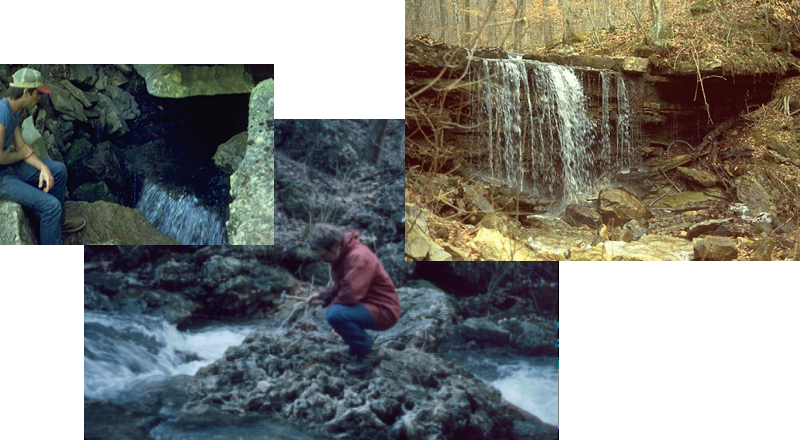
\includegraphics[width=0.75\linewidth]{img/waterSampling} 

}

\caption{Water sampling in varying lithologies in a karst area}\label{fig:statSinkingCoveSampling}
\end{figure}

We can look at this spatially (Figure \ref{fig:statSinkingCoveHardness}) as well as by variables graphically (Figure \ref{fig:statTHbyLithology}).

\begin{Shaded}
\begin{Highlighting}[]
\FunctionTok{library}\NormalTok{(igisci)}
\FunctionTok{library}\NormalTok{(sf); }\FunctionTok{library}\NormalTok{(tidyverse); }\FunctionTok{library}\NormalTok{(readxl); }\FunctionTok{library}\NormalTok{(tmap); }\FunctionTok{library}\NormalTok{(terra)}
\NormalTok{wChemData }\OtherTok{\textless{}{-}} \FunctionTok{read\_excel}\NormalTok{(}\FunctionTok{ex}\NormalTok{(}\StringTok{"SinkingCove/SinkingCoveWaterChem.xlsx"}\NormalTok{)) }\SpecialCharTok{\%\textgreater{}\%}
  \FunctionTok{mutate}\NormalTok{(}\AttributeTok{siteLoc =} \FunctionTok{str\_sub}\NormalTok{(Site,}\AttributeTok{start=}\DecValTok{1}\DataTypeTok{L}\NormalTok{, }\AttributeTok{end=}\DecValTok{1}\DataTypeTok{L}\NormalTok{))}
\NormalTok{wChemTrunk }\OtherTok{\textless{}{-}}\NormalTok{ wChemData }\SpecialCharTok{\%\textgreater{}\%} \FunctionTok{filter}\NormalTok{(siteLoc }\SpecialCharTok{==} \StringTok{"T"}\NormalTok{) }\SpecialCharTok{\%\textgreater{}\%} \FunctionTok{mutate}\NormalTok{(}\AttributeTok{siteType =} \StringTok{"trunk"}\NormalTok{)}
\NormalTok{wChemDrip }\OtherTok{\textless{}{-}}\NormalTok{ wChemData }\SpecialCharTok{\%\textgreater{}\%} \FunctionTok{filter}\NormalTok{(siteLoc }\SpecialCharTok{\%in\%} \FunctionTok{c}\NormalTok{(}\StringTok{"D"}\NormalTok{,}\StringTok{"S"}\NormalTok{)) }\SpecialCharTok{\%\textgreater{}\%} \FunctionTok{mutate}\NormalTok{(}\AttributeTok{siteType =} \StringTok{"dripwater"}\NormalTok{)}
\NormalTok{wChemTrib }\OtherTok{\textless{}{-}}\NormalTok{ wChemData }\SpecialCharTok{\%\textgreater{}\%} \FunctionTok{filter}\NormalTok{(siteLoc }\SpecialCharTok{\%in\%} \FunctionTok{c}\NormalTok{(}\StringTok{"B"}\NormalTok{, }\StringTok{"F"}\NormalTok{, }\StringTok{"K"}\NormalTok{, }\StringTok{"W"}\NormalTok{, }\StringTok{"P"}\NormalTok{)) }\SpecialCharTok{\%\textgreater{}\%} 
  \FunctionTok{mutate}\NormalTok{(}\AttributeTok{siteType =} \StringTok{"tributary"}\NormalTok{)}
\NormalTok{wChemData }\OtherTok{\textless{}{-}} \FunctionTok{bind\_rows}\NormalTok{(wChemTrunk, wChemDrip, wChemTrib)}
\NormalTok{wChemData}\SpecialCharTok{$}\NormalTok{siteType }\OtherTok{\textless{}{-}} \FunctionTok{factor}\NormalTok{(wChemData}\SpecialCharTok{$}\NormalTok{siteType)}
\NormalTok{wChemData}\SpecialCharTok{$}\NormalTok{Lithology }\OtherTok{\textless{}{-}} \FunctionTok{factor}\NormalTok{(wChemData}\SpecialCharTok{$}\NormalTok{Lithology)}
\NormalTok{sites }\OtherTok{\textless{}{-}} \FunctionTok{read\_csv}\NormalTok{(}\FunctionTok{ex}\NormalTok{(}\StringTok{"SinkingCove/SinkingCoveSites.csv"}\NormalTok{))}
\NormalTok{wChem }\OtherTok{\textless{}{-}}\NormalTok{ wChemData }\SpecialCharTok{\%\textgreater{}\%}
  \FunctionTok{left\_join}\NormalTok{(sites, }\AttributeTok{by =} \FunctionTok{c}\NormalTok{(}\StringTok{"Site"} \OtherTok{=} \StringTok{"site"}\NormalTok{)) }\SpecialCharTok{\%\textgreater{}\%}
  \FunctionTok{st\_as\_sf}\NormalTok{(}\AttributeTok{coords =} \FunctionTok{c}\NormalTok{(}\StringTok{"longitude"}\NormalTok{, }\StringTok{"latitude"}\NormalTok{), }\AttributeTok{crs =} \DecValTok{4326}\NormalTok{)}
\FunctionTok{tmap\_mode}\NormalTok{(}\StringTok{"plot"}\NormalTok{)}
\NormalTok{DEM }\OtherTok{\textless{}{-}} \FunctionTok{rast}\NormalTok{(}\FunctionTok{ex}\NormalTok{(}\StringTok{"SinkingCove/DEM\_SinkingCoveUTM.tif"}\NormalTok{))   }
\NormalTok{slope }\OtherTok{\textless{}{-}} \FunctionTok{terrain}\NormalTok{(DEM, }\AttributeTok{v=}\StringTok{\textquotesingle{}slope\textquotesingle{}}\NormalTok{)}
\NormalTok{aspect }\OtherTok{\textless{}{-}} \FunctionTok{terrain}\NormalTok{(DEM, }\AttributeTok{v=}\StringTok{\textquotesingle{}aspect\textquotesingle{}}\NormalTok{)}
\NormalTok{hillsh }\OtherTok{\textless{}{-}} \FunctionTok{shade}\NormalTok{(slope}\SpecialCharTok{/}\DecValTok{180}\SpecialCharTok{*}\NormalTok{pi, aspect}\SpecialCharTok{/}\DecValTok{180}\SpecialCharTok{*}\NormalTok{pi, }\DecValTok{40}\NormalTok{, }\DecValTok{330}\NormalTok{) }
\NormalTok{bounds }\OtherTok{\textless{}{-}}\NormalTok{ tmaptools}\SpecialCharTok{::}\FunctionTok{bb}\NormalTok{(wChem, }\AttributeTok{ext=}\FloatTok{1.1}\NormalTok{)}

\NormalTok{hillshCol }\OtherTok{\textless{}{-}} \FunctionTok{tm\_scale\_continuous}\NormalTok{(}\AttributeTok{values =} \StringTok{"{-}brewer.greys"}\NormalTok{)}
\NormalTok{terrainCol }\OtherTok{\textless{}{-}} \FunctionTok{tm\_scale\_continuous}\NormalTok{(}\AttributeTok{values =} \FunctionTok{terrain.colors}\NormalTok{(}\DecValTok{9}\NormalTok{))}

\FunctionTok{tm\_graticules}\NormalTok{(}\AttributeTok{labels.cardinal=}\NormalTok{F) }\SpecialCharTok{+}
  \FunctionTok{tm\_shape}\NormalTok{(hillsh,}\AttributeTok{bbox=}\NormalTok{bounds) }\SpecialCharTok{+}
    \FunctionTok{tm\_raster}\NormalTok{(}\AttributeTok{col.scale=}\NormalTok{hillshCol, }\AttributeTok{col.legend =} \FunctionTok{tm\_legend}\NormalTok{(}\AttributeTok{show=}\NormalTok{F)) }\SpecialCharTok{+} 
  \FunctionTok{tm\_shape}\NormalTok{(DEM) }\SpecialCharTok{+} 
    \FunctionTok{tm\_raster}\NormalTok{(}\AttributeTok{col.scale=}\NormalTok{terrainCol, }\AttributeTok{col\_alpha=}\FloatTok{0.5}\NormalTok{,}\AttributeTok{col.legend =} \FunctionTok{tm\_legend}\NormalTok{(}\AttributeTok{show=}\NormalTok{F)) }\SpecialCharTok{+}
  \FunctionTok{tm\_shape}\NormalTok{(wChem) }\SpecialCharTok{+}
    \FunctionTok{tm\_symbols}\NormalTok{(}\AttributeTok{size=}\StringTok{"TH"}\NormalTok{,}
               \AttributeTok{fill=}\StringTok{"Lithology"}\NormalTok{,}
               \FunctionTok{tm\_scale\_continuous}\NormalTok{(}\AttributeTok{values=}\FunctionTok{c}\NormalTok{(}\FloatTok{0.2}\NormalTok{,}\DecValTok{2}\NormalTok{)), }
               \AttributeTok{shape=}\StringTok{"siteType"}\NormalTok{, }
               \FunctionTok{tm\_legend}\NormalTok{(}\AttributeTok{frame=}\NormalTok{F)) }\SpecialCharTok{+}
  \FunctionTok{tm\_title}\NormalTok{(}\StringTok{"Upper Sinking Cove"}\NormalTok{)}
\end{Highlighting}
\end{Shaded}

\begin{figure}

{\centering 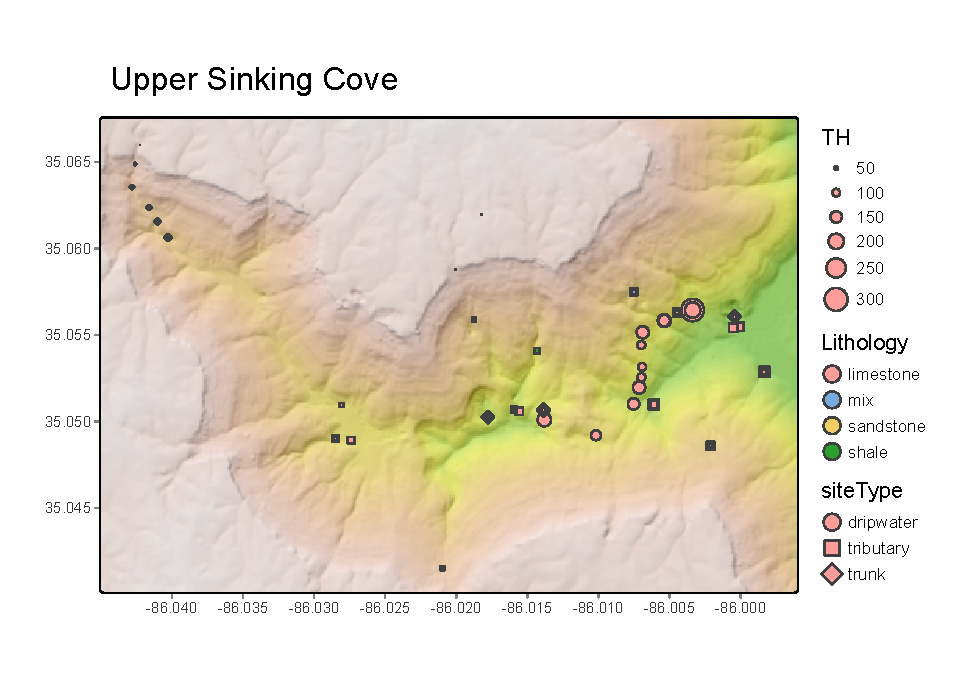
\includegraphics[width=0.75\linewidth]{EnvDataScience_files/figure-latex/statSinkingCoveHardness-1} 

}

\caption{Total hardness from dissolved carbonates at water sampling sites in Upper Sinking Cove, TN}\label{fig:statSinkingCoveHardness}
\end{figure}

Before we run the analysis of variance tests, we'll look at the data in another visual way, with histograms of total hardness, colored by site type, and faceted by lithology. We can already see that the groups are quite distinct, so there'll be no surprises revealed in the analysis of variance.

\begin{Shaded}
\begin{Highlighting}[]
\NormalTok{wChemData }\SpecialCharTok{\%\textgreater{}\%}
  \FunctionTok{ggplot}\NormalTok{(}\FunctionTok{aes}\NormalTok{(}\AttributeTok{x=}\NormalTok{TH, }\AttributeTok{fill=}\NormalTok{siteType)) }\SpecialCharTok{+}
  \FunctionTok{geom\_histogram}\NormalTok{() }\SpecialCharTok{+}
  \FunctionTok{facet\_grid}\NormalTok{(Lithology }\SpecialCharTok{\textasciitilde{}}\NormalTok{ .)}
\end{Highlighting}
\end{Shaded}

\begin{figure}

{\centering 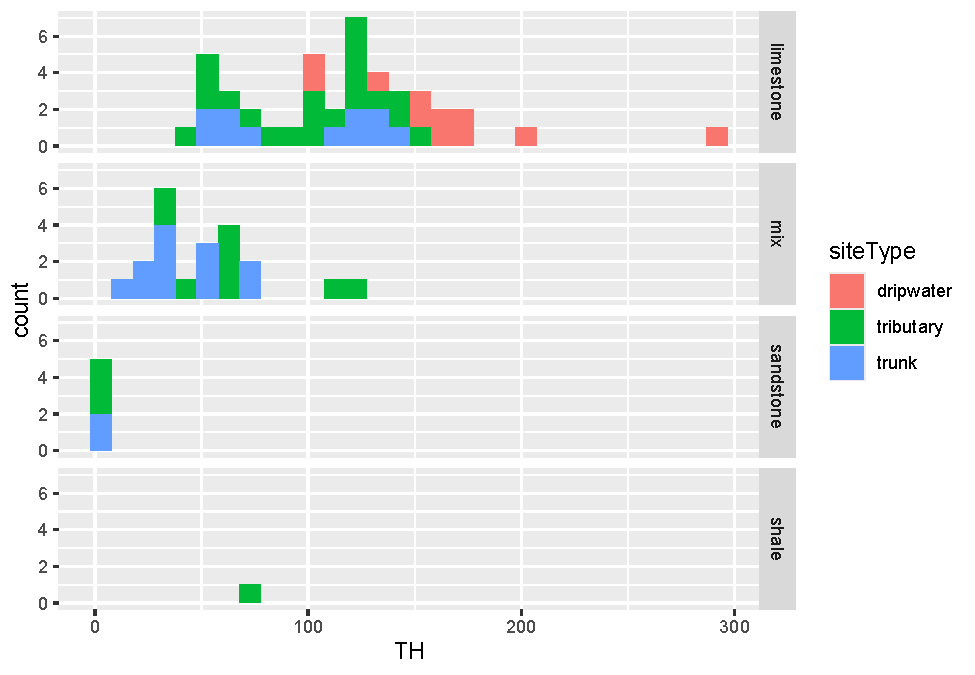
\includegraphics[width=0.75\linewidth]{EnvDataScience_files/figure-latex/statTHbyLithology-1} 

}

\caption{Sinking Cove dissolved carbonates as total hardness by lithology}\label{fig:statTHbyLithology}
\end{figure}

\textbf{Analysis of Variance}: An analysis of variance is run the same way as a linear model, and in fact you can sometimes use \texttt{lm()} instead of \texttt{aov()}, but the latter has advantages when checking the assumptions required for the model. Then the \texttt{anova()} function just displays the Analysis of Variance table, but you can see the same thing with \texttt{summary()}. You'll find practitioners vary in their practice, so it can be confusing. We'll start with deriving the model for total hardness to assess the factor \texttt{siteType}.

\begin{Shaded}
\begin{Highlighting}[]
\NormalTok{aov\_THsite }\OtherTok{\textless{}{-}} \FunctionTok{aov}\NormalTok{(TH}\SpecialCharTok{\textasciitilde{}}\NormalTok{siteType, }\AttributeTok{data =}\NormalTok{ wChemData)}
\FunctionTok{anova}\NormalTok{(aov\_THsite)}
\end{Highlighting}
\end{Shaded}

\begin{verbatim}
## Analysis of Variance Table
## 
## Response: TH
##           Df Sum Sq Mean Sq F value    Pr(>F)    
## siteType   2  79172   39586   20.59 1.071e-07 ***
## Residuals 67 128815    1923                      
## ---
## Signif. codes:  0 '***' 0.001 '**' 0.01 '*' 0.05 '.' 0.1 ' ' 1
\end{verbatim}

\begin{Shaded}
\begin{Highlighting}[]
\FunctionTok{summary}\NormalTok{(aov\_THsite)}
\end{Highlighting}
\end{Shaded}

\begin{verbatim}
##             Df Sum Sq Mean Sq F value   Pr(>F)    
## siteType     2  79172   39586   20.59 1.07e-07 ***
## Residuals   67 128815    1923                     
## ---
## Signif. codes:  0 '***' 0.001 '**' 0.01 '*' 0.05 '.' 0.1 ' ' 1
\end{verbatim}

So it seems that grouping by siteType is significant. To consider the validity of assumptions, we'll start by checking that the variances are homogeneous, required for analysis of variance. This can be tested by looking for any relationship between residuals and fitted values, using the base plot system that knows what to do for this type of model, with option 1 plotting residuals against fitted values.

\begin{Shaded}
\begin{Highlighting}[]
\FunctionTok{plot}\NormalTok{(aov\_THsite, }\DecValTok{1}\NormalTok{)}
\end{Highlighting}
\end{Shaded}

\begin{center}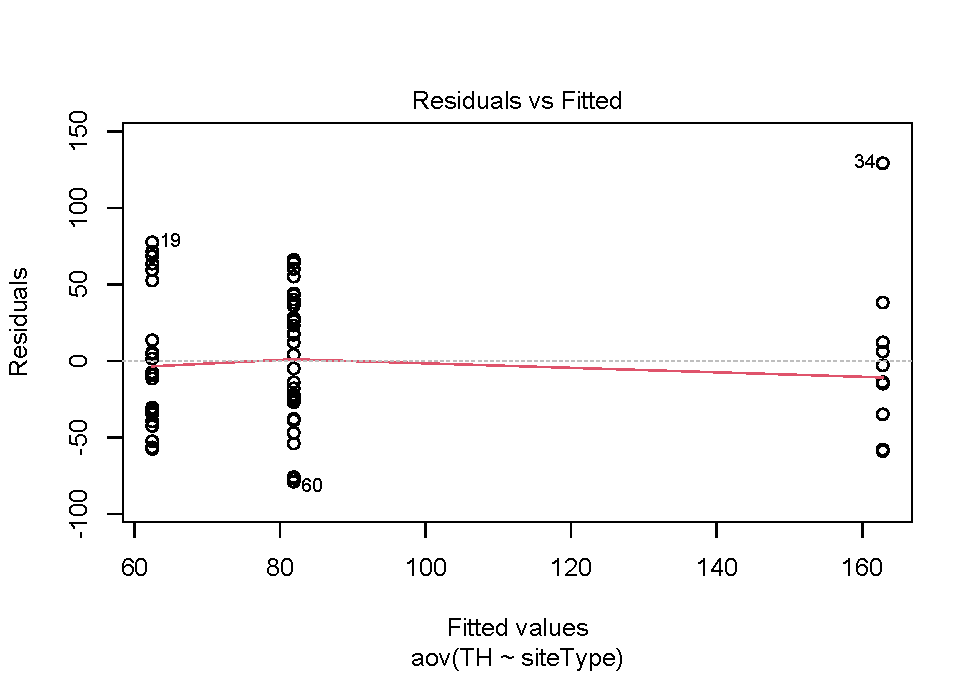
\includegraphics[width=0.75\linewidth]{EnvDataScience_files/figure-latex/unnamed-chunk-263-1} \end{center}

So that looks good, with no apparent relationship. Then we'll check for normality of residuals with a Q-Q plot, option 2 when plotting this type of model. It should approximate a straight line, which it does reasonably well.

\begin{Shaded}
\begin{Highlighting}[]
\FunctionTok{plot}\NormalTok{(aov\_THsite, }\DecValTok{2}\NormalTok{)}
\end{Highlighting}
\end{Shaded}

\begin{center}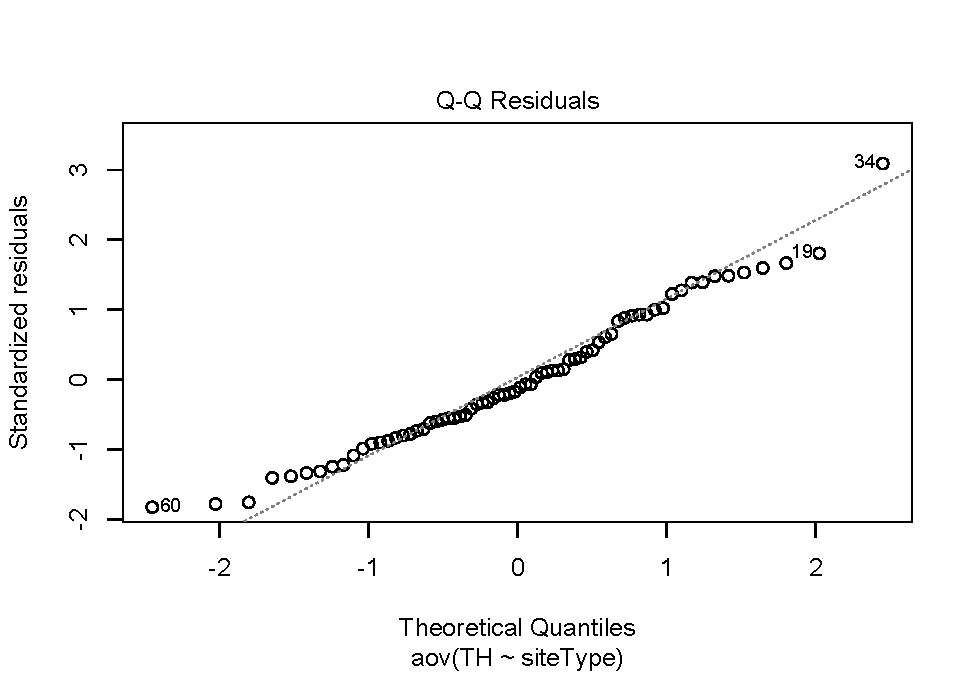
\includegraphics[width=0.75\linewidth]{EnvDataScience_files/figure-latex/unnamed-chunk-264-1} \end{center}

\subsection{Post-Hoc Analysis of Variance with Tukey's Test}\label{post-hoc-analysis-of-variance-with-tukeys-test}

``Post-Hoc Analysis'' refers to analyzing a model that has been created, and one method for this with an analysis of variance model is the Tukey ``Honest Significant Difference'' method provided by the base R function \texttt{TukeyHSD()}. This is from the same John Tukey who we looked at earlier as a promoter of \emph{exploratory data analysis} including visualization methods such as the Tukey boxplot.

One thing the \texttt{TukeyHSD()} function does is compare all group pairings. If you only have two groups, the form of the output will look the same, but we have three groups, so let's see what it shows. To run the test, we just provide our analysis of variance model \texttt{aov\_THsite} to the function \texttt{TukeyHSD()}, with a confidence level.

\begin{Shaded}
\begin{Highlighting}[]
\FunctionTok{TukeyHSD}\NormalTok{(aov\_THsite, }\AttributeTok{conf.level=}\NormalTok{.}\DecValTok{95}\NormalTok{)}
\end{Highlighting}
\end{Shaded}

\begin{verbatim}
##   Tukey multiple comparisons of means
##     95% family-wise confidence level
## 
## Fit: aov(formula = TH ~ siteType, data = wChemData)
## 
## $siteType
##                           diff        lwr        upr     p adj
## tributary-dripwater  -80.93583 -117.39136 -44.480301 0.0000038
## trunk-dripwater     -100.37818 -138.40394 -62.352427 0.0000001
## trunk-tributary      -19.44235  -47.13149   8.246788 0.2191791
\end{verbatim}

And here we see a surprise (though it shouldn't really be a surprise if we look at the data): while dripwater is distinct from the other two, there's no significant difference between trunk and tributary samples. This shouldn't be a surprise since both trunk and tributary sources are flowing streams, while the dripwaters come from soils above via bedrock where they're dissolving the calcium carbonate.

We'll do the same thing for the geology (or more specifically, lithology, which is rock type).

\begin{Shaded}
\begin{Highlighting}[]
\NormalTok{aov\_THlith }\OtherTok{\textless{}{-}} \FunctionTok{aov}\NormalTok{(TH}\SpecialCharTok{\textasciitilde{}}\NormalTok{Lithology, }\AttributeTok{data =}\NormalTok{ wChemData)}
\FunctionTok{anova}\NormalTok{(aov\_THlith)}
\end{Highlighting}
\end{Shaded}

\begin{verbatim}
## Analysis of Variance Table
## 
## Response: TH
##           Df Sum Sq Mean Sq F value    Pr(>F)    
## Lithology  3  98107   32702  19.643 3.278e-09 ***
## Residuals 66 109881    1665                      
## ---
## Signif. codes:  0 '***' 0.001 '**' 0.01 '*' 0.05 '.' 0.1 ' ' 1
\end{verbatim}

This grouping also appears significant, but let's also try the TukeyHSD test:

\begin{Shaded}
\begin{Highlighting}[]
\FunctionTok{TukeyHSD}\NormalTok{(aov\_THlith, }\AttributeTok{conf.level=}\NormalTok{.}\DecValTok{95}\NormalTok{ )}
\end{Highlighting}
\end{Shaded}

\begin{verbatim}
##   Tukey multiple comparisons of means
##     95% family-wise confidence level
## 
## Fit: aov(formula = TH ~ Lithology, data = wChemData)
## 
## $Lithology
##                           diff        lwr        upr     p adj
## mix-limestone        -65.76523  -94.39604 -37.134411 0.0000004
## sandstone-limestone -110.86047 -161.67512 -60.045808 0.0000015
## shale-limestone      -38.86047 -147.64815  69.927216 0.7826397
## sandstone-mix        -45.09524  -98.61074   8.420267 0.1281941
## shale-mix             26.90476  -83.17039 136.979916 0.9171930
## shale-sandstone       72.00000  -45.80894 189.808935 0.3796721
\end{verbatim}

That shows something useful: the only pairing that is significantly distinct is between sandstone and limestone. This is also not surprising because all of the sandstone is on the caprock so there's no direct source of carbonates and none from upstream.

Again considering assumptions, for homogeneity of variances, there's no apparent relationship between residuals and fitted values:

\begin{Shaded}
\begin{Highlighting}[]
\FunctionTok{plot}\NormalTok{(aov\_THlith, }\DecValTok{1}\NormalTok{)}
\end{Highlighting}
\end{Shaded}

\begin{center}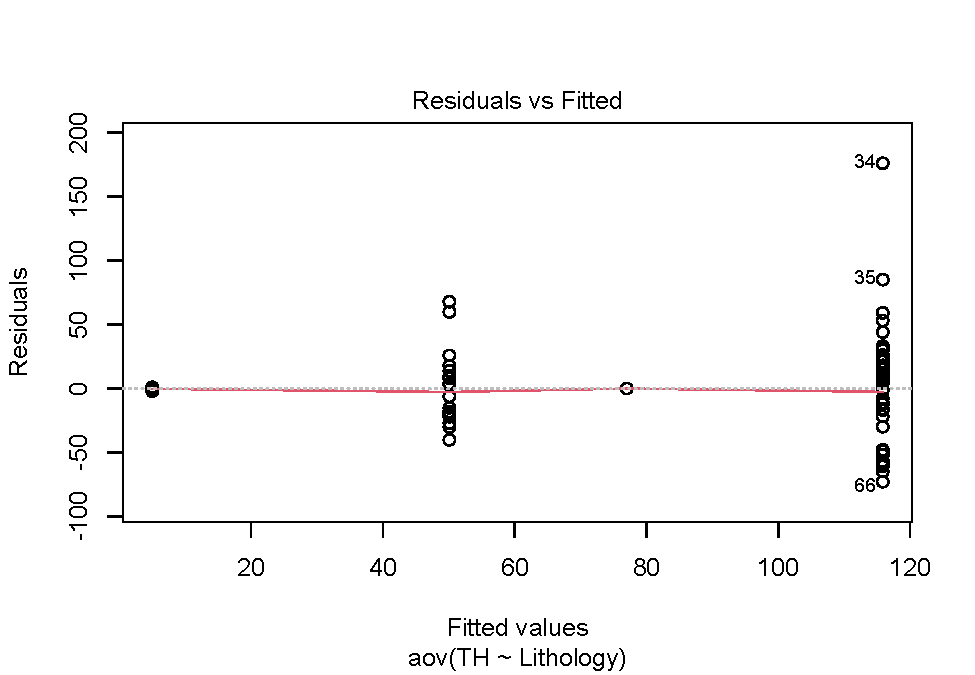
\includegraphics[width=0.75\linewidth]{EnvDataScience_files/figure-latex/unnamed-chunk-268-1} \end{center}

And the Q-Q plot's reasonable approximation of a straight line supports the assumption that the residuals are normally distributed.

\begin{Shaded}
\begin{Highlighting}[]
\FunctionTok{plot}\NormalTok{(aov\_THlith, }\DecValTok{2}\NormalTok{)}
\end{Highlighting}
\end{Shaded}

\begin{center}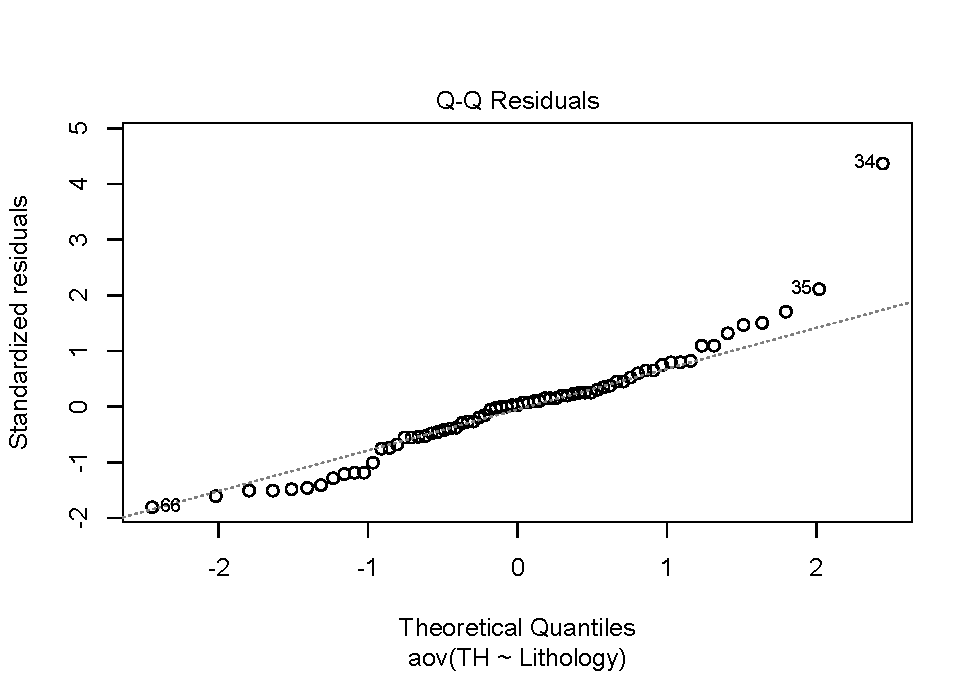
\includegraphics[width=0.75\linewidth]{EnvDataScience_files/figure-latex/unnamed-chunk-269-1} \end{center}

Some observations and caveats from the above:

\begin{itemize}
\tightlist
\item
  There's pretty clearly a difference between surface waters (trunk and tributary) and cave dripwaters (from stalactites) in terms of solutes. Analysis of variance simply confirms the obvious.
\item
  There's also pretty clearly a difference among lithologies on the basis of solutes, not surprising since limestone is much more soluble than sandstones. Similarly, analysis of variance confirms the obvious.
\item
  The data may not be sufficiently normally distributed, and limestone hardness values are bimodal (largely due to the inaccessibility of waters in the trunk cave passages traveling 2 km through the Bangor limestone \footnote{We tried very hard to get into that cave that must extend from upper Cave Cove then under Farmer Cove to a spring in Wolf Cove -- we have dye traces to prove it.}), though analysis of variance may be less sensitive to this than a t test.
\item
  While shale creates springs, shale strata are very thin, with most of them in the ``mix'' category, or form the boundary between the two major limestone formations. Tributary streams appear to cross the shale in caves that were inaccessible for sampling. We visually confirmed this in one cave, but this exploration required some challenging rappel work to access, so we were not able to sample.
\item
  The geologic structure \index{geology} here is essentially flat, with sandstones on the plateau surface and the most massive limestones -- the Bangor and Monteagle limestones -- all below 400 m elevation (Figure \ref{fig:statSinkingCoveStrat}).
\end{itemize}

\begin{figure}

{\centering 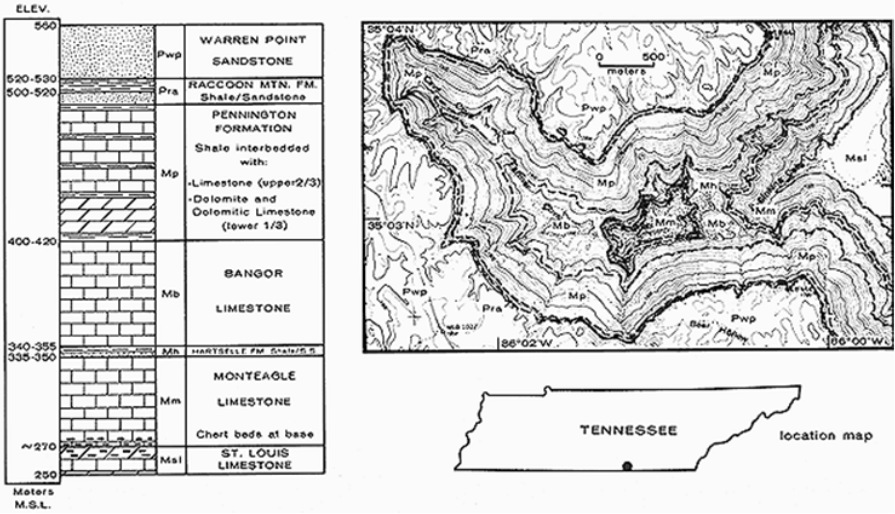
\includegraphics[width=0.9\linewidth]{img/UpperSinkingCoveGeology} 

}

\caption{Upper Sinking Cove (Tennessee) stratigraphy}\label{fig:statSinkingCoveStrat}
\end{figure}

\begin{itemize}
\tightlist
\item
  While the rapid increase in solutes happens when Cave Cove Creek starts draining through the much more soluble limestone until it reaches saturation, the distance traveled by the water (reflected by a drop in elevation) can be seen (Figure \ref{fig:statSinkingCoveTHelevLith}).
\end{itemize}

\begin{Shaded}
\begin{Highlighting}[]
\NormalTok{wChemData }\SpecialCharTok{\%\textgreater{}\%}
  \FunctionTok{ggplot}\NormalTok{(}\FunctionTok{aes}\NormalTok{(}\AttributeTok{x=}\NormalTok{Elevation, }\AttributeTok{y=}\NormalTok{TH, }\AttributeTok{col=}\NormalTok{Lithology)) }\SpecialCharTok{+} 
  \FunctionTok{geom\_point}\NormalTok{() }\SpecialCharTok{+} 
  \FunctionTok{geom\_smooth}\NormalTok{(}\AttributeTok{method=} \StringTok{"lm"}\NormalTok{)}
\end{Highlighting}
\end{Shaded}

\begin{figure}

{\centering 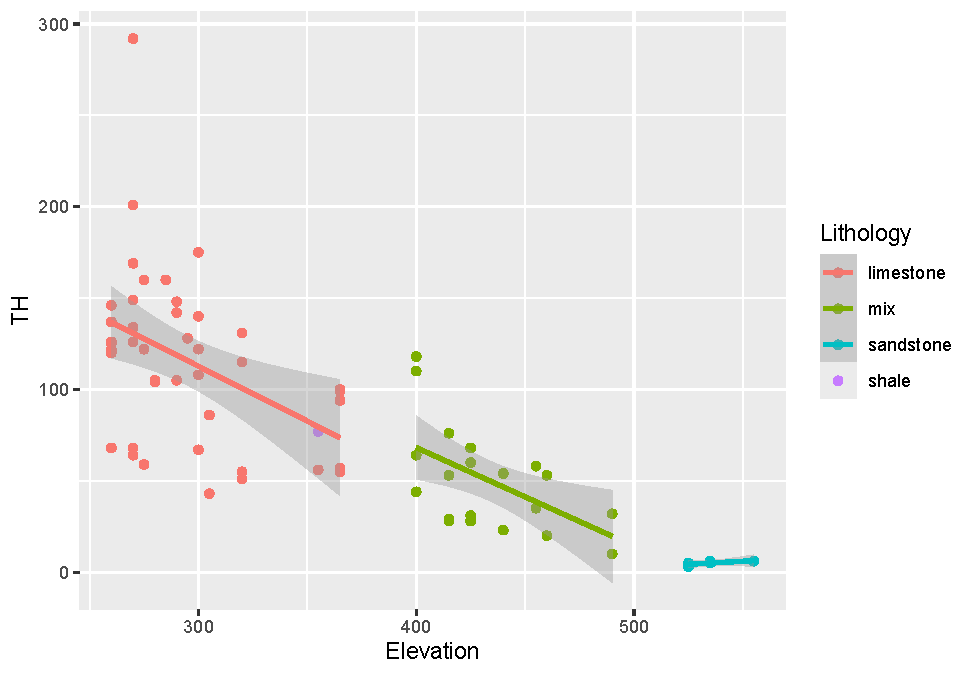
\includegraphics[width=0.75\linewidth]{EnvDataScience_files/figure-latex/statSinkingCoveTHelevLith-1} 

}

\caption{Sinking Cove dissolved carbonates as TH and elevation by lithology}\label{fig:statSinkingCoveTHelevLith}
\end{figure}

\begin{quote}
As with other topics in these statistical chapters, there's a lot more to learn, but fortunately there are many resources on statistical methods, since they cut across so many sciences. A more thorough coverage of the use of the one-way ANOVA test can be found at \url{http://www.sthda.com/english/wiki/one-way-anova-test-in-r}. There's also an example applied to the palmerpenguins data set we've used before, in this blog: \url{https://statsandr.com/blog/anova-in-r} and many others.
\end{quote}

\subsection{Testing a correlation}\label{testing-a-correlation}

\index{correlation test}\index{cor.test}We earlier looked at the correlation coefficient r. One test we can do is to see whether that correlation is significant:

\begin{Shaded}
\begin{Highlighting}[]
\FunctionTok{cor.test}\NormalTok{(sierraFeb}\SpecialCharTok{$}\NormalTok{TEMPERATURE, sierraFeb}\SpecialCharTok{$}\NormalTok{ELEVATION)}
\end{Highlighting}
\end{Shaded}

\begin{verbatim}
## 
##  Pearson's product-moment correlation
## 
## data:  sierraFeb$TEMPERATURE and sierraFeb$ELEVATION
## t = -20.558, df = 60, p-value < 2.2e-16
## alternative hypothesis: true correlation is not equal to 0
## 95 percent confidence interval:
##  -0.9609478 -0.8952592
## sample estimates:
##        cor 
## -0.9357801
\end{verbatim}

So we can reject the null hypothesis that the correlation is equal to zero: the probability of getting a correlation of -0.936 is less than \(2.2\times 10^{-16}\) and thus the ``true correlation is not equal to 0''. So we can accept an alternative \emph{working hypothesis} that they're negatively correlated, and that -- no surprise -- \emph{it gets colder as we go to higher elevations}, at least in February in the Sierra, where our data come from.

In the next chapter, we'll use this data to develop a linear model and get a similar result comparing the slope of the model predicting temperature from elevation\ldots{}

\subsection{Additional resources}\label{additional-resources}

As you might expect, there are \emph{lots} of good statistical references based on R.

One book also published at bookdown.org is Paula Moraga's \emph{Spatial Statistics for Data Science} (2023) available at \url{https://www.paulamoraga.com/book-spatial/index.html}.

\pagebreak

\section{Exercises: Statistics}\label{exercises-statistics}

\begin{exercise}

Build a \texttt{soilvegJuly} data frame.

\begin{itemize}
\tightlist
\item
  Create a new RStudio project named Meadows.
\item
  Create a soilveg tibble from ``meadows/SoilVegSamples.csv'' in the extdata.
\item
  Have a look at this data frame and note that there is NA for SoilMoisture and NDVI for 8 of the records. These represent observations made in August, while the rest are all in July. While we have drone imagery and thus NDVI for these sites, as they are during the senescent period we don't want to compare these with the July samples.
\item
  Filter the data frame to only include records that are not NA (see 3.4.2.1) for SoilMoisture, and assign that to a new data frame \texttt{soilvegJuly}.
\end{itemize}

\end{exercise}

\begin{exercise}

Visualizations:

Using graphical methods you learned in Chapter 4:

\begin{itemize}
\tightlist
\item
  Create a scatter plot of Soil Moisture vs NDVI, colored by veg (the three-character abbreviation of major vegetation types -- \texttt{CAR} for Carex/sedge, \texttt{JUN} for Juncus/rush, \texttt{GRA} for mesic grasses and forbs, and \texttt{UPL} for more elevated (maybe by a meter) areas of sagebrush), for \texttt{soilvegJuly}. What we can see is that this is a small sample. This study involved a lot of drone imagery, probably 100s of GB of imagery, which was the main focus of the study -- to detect channels -- but a low density of soil and vegetation ground samples.
\item
  Create a histogram of soil moisture colored by veg, also for the July data. We see the same story, with not very many samples, though suggestive of a multimodal distribution overall.
\item
  Create a density plot of the same, using alpha = 0.5 to see everything with transparency.
\end{itemize}

\begin{quote}
You can also use DominantVegetation, for this and the next question. The results may be a bit different.
\end{quote}

\end{exercise}

\begin{center}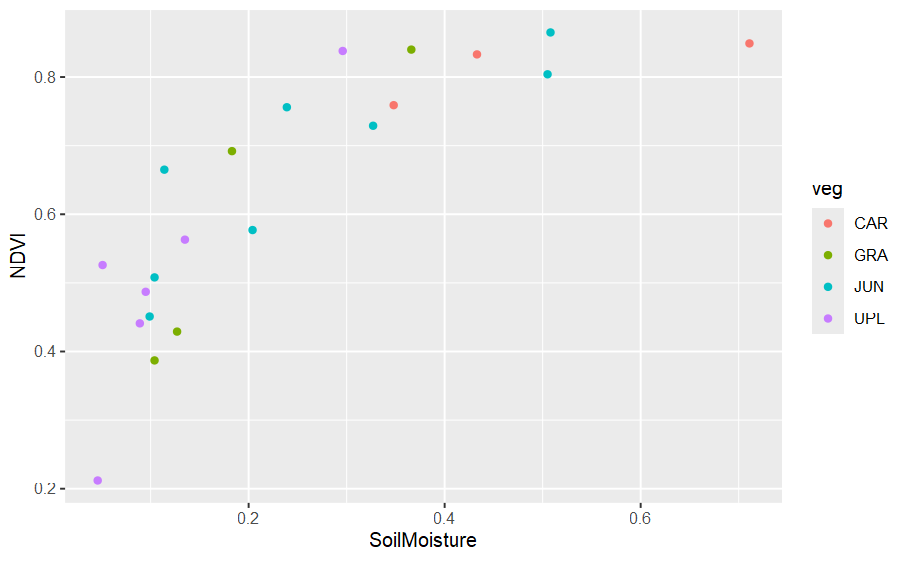
\includegraphics[width=0.75\linewidth]{img/stats_ex2a} \end{center}

\begin{center}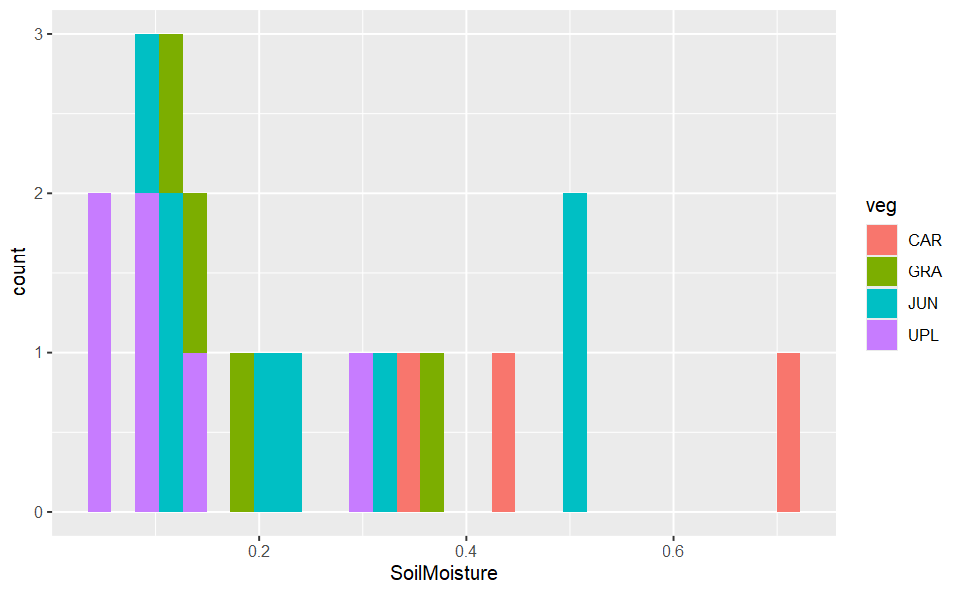
\includegraphics[width=0.75\linewidth]{img/stats_ex2b} \end{center}

\begin{center}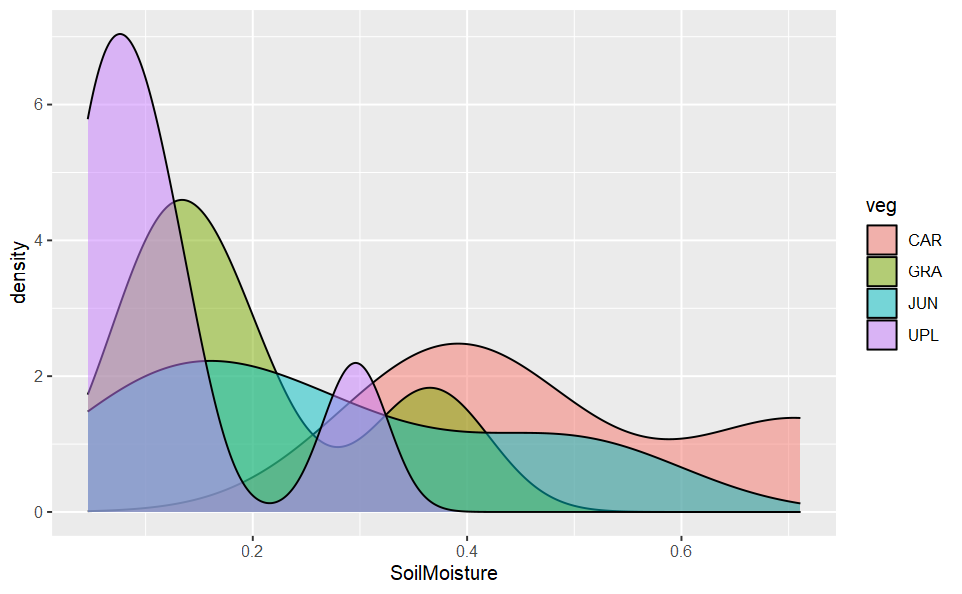
\includegraphics[width=0.75\linewidth]{img/stats_ex2c} \end{center}

\begin{exercise}
Tests, July data

Using methods from 9.4.2, run an analysis of variance test of soil moisture \textasciitilde{} veg. Remember to specify the data, which should be just the July data., then do the same test for NDVI \textasciitilde{} veg. Interpret the results in a markdown section.
\end{exercise}

\begin{exercise}

Meadow differences

\begin{itemize}
\tightlist
\item
  Now compare the meadows based on soil moisture in July, using a boxplot
\item
  Then run an ANOVA test on this meadow grouping
\end{itemize}

\end{exercise}

\begin{center}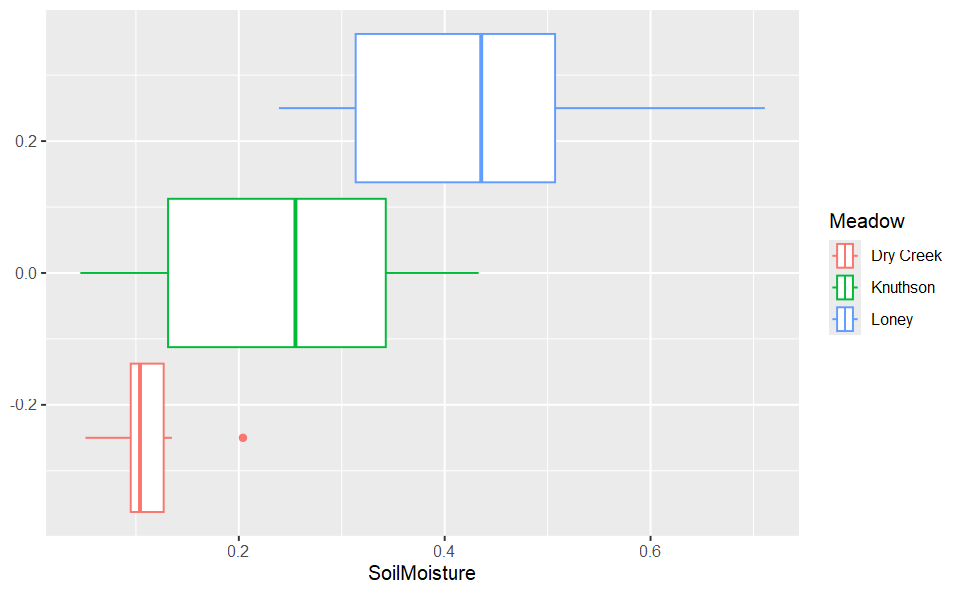
\includegraphics[width=0.75\linewidth]{img/stats_ex4} \end{center}

\begin{exercise}
For the meadow data, create a pairs plot to find which variables are correlated along with their r values, and test the significance of that correlation and provide percentage of variation of one variable is explained by that of the other.
\end{exercise}

\begin{center}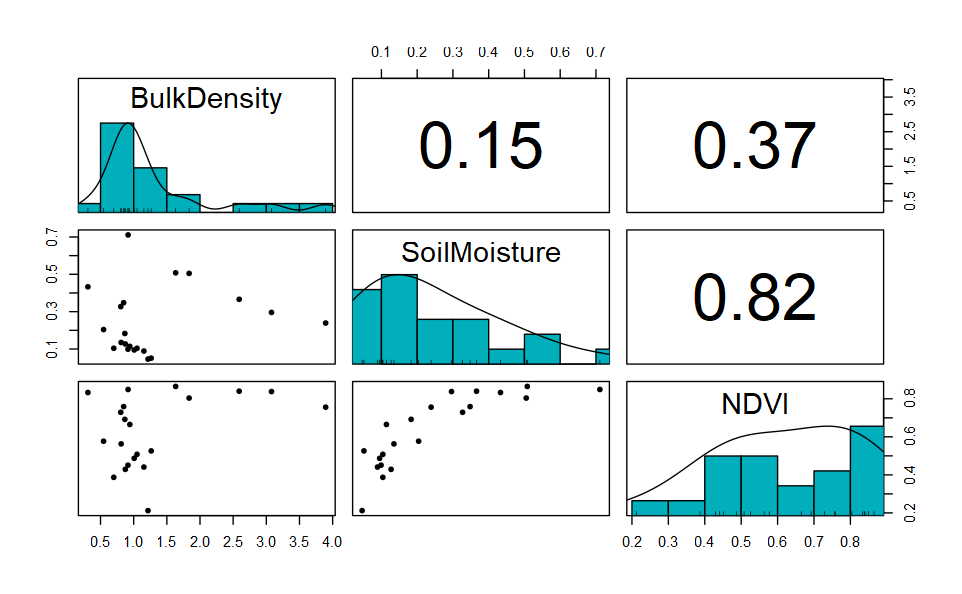
\includegraphics[width=0.75\linewidth]{img/stats_ex5} \end{center}

\begin{exercise}
Bulk density test, all data

We'll now look at bulk density for all samples (soilveg), including both July and August. Soil moisture and NDVI won't be a part of this analysis, only bulk density and vegetation. Look at the distribution of all bulk density values, using both a histogram with 20 bins and a density plot, then run an ANOVA test of bulk density predicted by (\textasciitilde) veg. What does the Pr(\textgreater F) value indicate?
\end{exercise}

\begin{exercise}
Carex or not?

Derive a bulkDensityCAR data frame by mutating a new variable CAR derived as a boolean result of \texttt{veg\ ==\ "CAR"}. This will group the vegetation points as either Carex or not, then use that in another ANOVA test to predict bulk density. What does the Pr(\textgreater F) value indicate?
\end{exercise}

\chapter{Modeling}\label{modeling}

\begin{center}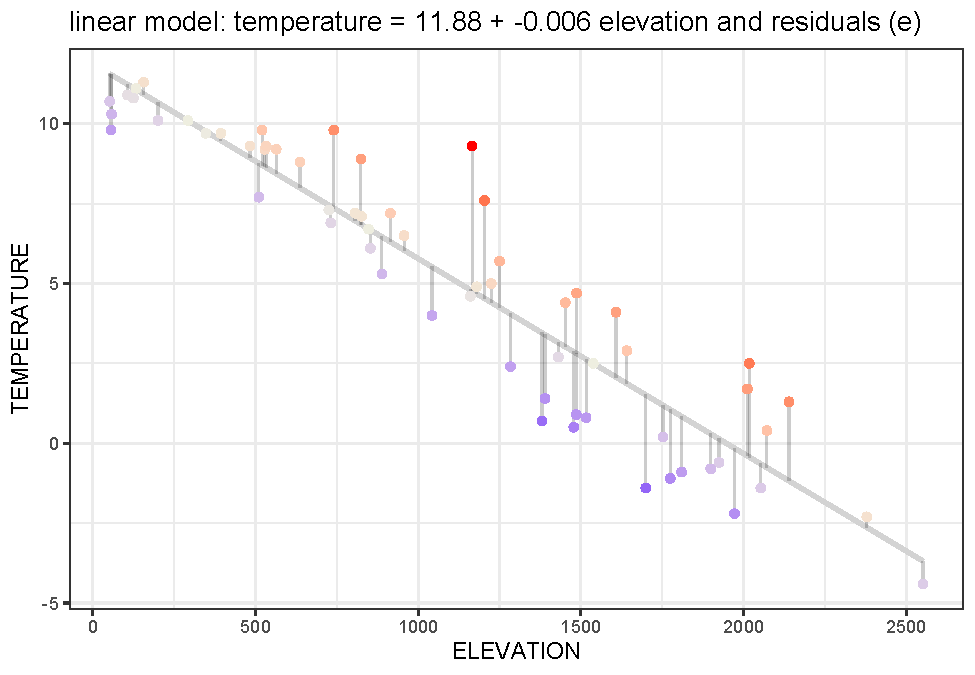
\includegraphics[width=0.75\linewidth]{EnvDataScience_files/figure-latex/ModelingChapter-1} \end{center}

\index{modeling}The purpose of a statistical model\index{statistical model} is to help understand what variables might best predict a phenomenon of interest, which ones have more or less influence, define a predictive equation with coefficients for each of the variables, and then apply that equation to predict values using the same input variables for other areas. This process requires samples with observations of the explanatory\index{explanatory variable} (or independent\index{independent variable}) and response\index{response variable} (or dependent\index{dependent variable}) variables in question.

\section{Some Common Statistical Models}\label{some-common-statistical-models}

There are many types of statistical models. Variables may be nominal (categorical) or interval/ratio data. You may be interested in predicting a continuous interval/ratio variable from other continuous variables, or predicting the probability of an occurrence (e.g.~of a species), or maybe the count of something (also maybe a species). You may be needing to classify your phenomena based on continuous variables. \index{lm linear model}\index{glm generalized linear model}\index{aov}\index{gam}\index{tree}Here are some examples:

\begin{itemize}
\tightlist
\item
  \texttt{lm(y\ \textasciitilde{}\ x)} linear regression model with one explanatory variable
\item
  \texttt{lm(y\ \textasciitilde{}\ x1\ +\ x2\ +\ x3)} multiple regression, a linear model with multiple explanatory variables
\item
  \texttt{glm(y\ \textasciitilde{}\ x,\ family\ =\ poisson)} generalized linear model, poisson distribution; see ?family to see those supported, including binomial, gaussian, poisson, etc.
\item
  \texttt{glm(y\ \textasciitilde{}\ x\ +\ y,\ family\ =\ binomial)} glm for logistic regression
\item
  \texttt{aov(y\ \textasciitilde{}\ x)} analysis of variance (same as lm except in the summary)
\item
  \texttt{gam(y\ \textasciitilde{}\ x)} generalized additive models
\item
  \texttt{tree(y\ \textasciitilde{}\ x)} or \texttt{rpart(y\ \textasciitilde{}\ x)} regression/classification trees
\end{itemize}

\section{\texorpdfstring{Linear Model (\texttt{lm})}{Linear Model (lm)}}\label{lm}

\index{linear model lm}If we look at the Sierra February climate example, the regression line in the graph above shows the response variable temperature predicted by the explanatory variable elevation. Here's the code that produced the model and graph:

\begin{Shaded}
\begin{Highlighting}[]
\FunctionTok{library}\NormalTok{(igisci); }\FunctionTok{library}\NormalTok{(tidyverse)}
\NormalTok{sierra }\OtherTok{\textless{}{-}}\NormalTok{ sierraFeb }\SpecialCharTok{\%\textgreater{}\%}
  \FunctionTok{filter}\NormalTok{(}\SpecialCharTok{!}\FunctionTok{is.na}\NormalTok{(TEMPERATURE))}
\NormalTok{model1 }\OtherTok{=} \FunctionTok{lm}\NormalTok{(TEMPERATURE }\SpecialCharTok{\textasciitilde{}}\NormalTok{ ELEVATION, }\AttributeTok{data =}\NormalTok{ sierra)}
\NormalTok{cc }\OtherTok{=}\NormalTok{ model1}\SpecialCharTok{$}\NormalTok{coefficients}
\NormalTok{sierra}\SpecialCharTok{$}\NormalTok{resid }\OtherTok{=} \FunctionTok{resid}\NormalTok{(model1)}
\NormalTok{sierra}\SpecialCharTok{$}\NormalTok{predict }\OtherTok{=} \FunctionTok{predict}\NormalTok{(model1) }
\NormalTok{eqn }\OtherTok{=} \FunctionTok{paste}\NormalTok{(}\StringTok{"temperature ="}\NormalTok{, }
\NormalTok{            (}\FunctionTok{round}\NormalTok{(cc[}\DecValTok{1}\NormalTok{], }\AttributeTok{digits=}\DecValTok{2}\NormalTok{)), }\StringTok{"+"}\NormalTok{,  }
\NormalTok{            (}\FunctionTok{round}\NormalTok{(cc[}\DecValTok{2}\NormalTok{], }\AttributeTok{digits=}\DecValTok{3}\NormalTok{)), }\StringTok{"elevation + e"}\NormalTok{)}
\FunctionTok{ggplot}\NormalTok{(sierra, }\FunctionTok{aes}\NormalTok{(}\AttributeTok{x=}\NormalTok{ELEVATION, }\AttributeTok{y=}\NormalTok{TEMPERATURE)) }\SpecialCharTok{+} 
  \FunctionTok{geom\_smooth}\NormalTok{(}\AttributeTok{method=}\StringTok{"lm"}\NormalTok{, }\AttributeTok{se=}\ConstantTok{FALSE}\NormalTok{, }\AttributeTok{color=}\StringTok{"lightgrey"}\NormalTok{) }\SpecialCharTok{+}
  \FunctionTok{geom\_segment}\NormalTok{(}\FunctionTok{aes}\NormalTok{(}\AttributeTok{xend=}\NormalTok{ELEVATION, }\AttributeTok{yend=}\NormalTok{predict), }\AttributeTok{alpha=}\NormalTok{.}\DecValTok{2}\NormalTok{) }\SpecialCharTok{+}
  \FunctionTok{geom\_point}\NormalTok{(}\FunctionTok{aes}\NormalTok{(}\AttributeTok{color=}\NormalTok{resid)) }\SpecialCharTok{+}
  \FunctionTok{scale\_color\_gradient2}\NormalTok{(}\AttributeTok{low=}\StringTok{"blue"}\NormalTok{, }\AttributeTok{mid=}\StringTok{"ivory2"}\NormalTok{, }\AttributeTok{high=}\StringTok{"red"}\NormalTok{) }\SpecialCharTok{+}
  \FunctionTok{guides}\NormalTok{(}\AttributeTok{color=}\StringTok{"none"}\NormalTok{) }\SpecialCharTok{+}
  \FunctionTok{theme\_bw}\NormalTok{() }\SpecialCharTok{+}
  \FunctionTok{ggtitle}\NormalTok{(}\FunctionTok{paste}\NormalTok{(}\StringTok{"Residuals (e) from model: "}\NormalTok{,eqn))}
\end{Highlighting}
\end{Shaded}

The \texttt{summary()} \index{summary for model results}function can be used to look at the results statistically:

\begin{Shaded}
\begin{Highlighting}[]
\FunctionTok{summary}\NormalTok{(model1)}
\end{Highlighting}
\end{Shaded}

\begin{verbatim}
## 
## Call:
## lm(formula = TEMPERATURE ~ ELEVATION, data = sierra)
## 
## Residuals:
##     Min      1Q  Median      3Q     Max 
## -2.9126 -1.0466 -0.0027  0.7940  4.5327 
## 
## Coefficients:
##               Estimate Std. Error t value Pr(>|t|)    
## (Intercept) 11.8813804  0.3825302   31.06   <2e-16 ***
## ELEVATION   -0.0061018  0.0002968  -20.56   <2e-16 ***
## ---
## Signif. codes:  0 '***' 0.001 '**' 0.01 '*' 0.05 '.' 0.1 ' ' 1
## 
## Residual standard error: 1.533 on 60 degrees of freedom
## Multiple R-squared:  0.8757, Adjusted R-squared:  0.8736 
## F-statistic: 422.6 on 1 and 60 DF,  p-value: < 2.2e-16
\end{verbatim}

Probably the most important statistic is the \index{p}p value for the coefficient of the explanatory variable \texttt{ELEVATION}, which in this case is very small: \(<2.2\times10^{-16}\).

The graph shows not only the linear prediction line, but also the scatter plot of input points displayed with connecting offsets indicating the magnitude of the residual (error term) of the data point away from the prediction.

\textbf{Making Predictions}

\index{predictive model}We can use the linear equation and the coefficients derived for the intercept and the explanatory variable (and rounded a bit) to predict temperatures given the explanatory variable elevation, so:

\[
Temperature_{prediction} = 11.88 - 0.006{elevation}
\]

So with these coefficients\index{model coefficients}, we can apply the equation to a vector of elevations to predict temperature from those elevations:

\begin{Shaded}
\begin{Highlighting}[]
\NormalTok{b0 }\OtherTok{\textless{}{-}}\NormalTok{ model1}\SpecialCharTok{$}\NormalTok{coefficients[}\DecValTok{1}\NormalTok{]}
\NormalTok{b1 }\OtherTok{\textless{}{-}}\NormalTok{ model1}\SpecialCharTok{$}\NormalTok{coefficients[}\DecValTok{2}\NormalTok{]}
\NormalTok{elevations }\OtherTok{\textless{}{-}} \FunctionTok{c}\NormalTok{(}\DecValTok{500}\NormalTok{, }\DecValTok{1000}\NormalTok{, }\DecValTok{1500}\NormalTok{, }\DecValTok{2000}\NormalTok{)}
\NormalTok{elevations}
\end{Highlighting}
\end{Shaded}

\begin{verbatim}
## [1]  500 1000 1500 2000
\end{verbatim}

\begin{Shaded}
\begin{Highlighting}[]
\NormalTok{tempEstimate }\OtherTok{\textless{}{-}}\NormalTok{ b0 }\SpecialCharTok{+}\NormalTok{ b1 }\SpecialCharTok{*}\NormalTok{ elevations}
\NormalTok{tempEstimate}
\end{Highlighting}
\end{Shaded}

\begin{verbatim}
## [1]  8.8304692  5.7795580  2.7286468 -0.3222645
\end{verbatim}

Next, we'll plot predictions and residuals on a map.

\section{Spatial Influences on Statistical Analysis}\label{spatial-influences-on-statistical-analysis}

\index{spatial influences on statistical analysis}Spatial statistical analysis brings in the spatial dimension to a statistical analysis, ranging from visual analysis of patterns to specialized spatial statistical methods. There are many applications for these methods in environmental research, since spatial patterns are generally highly relevant. We might ask:

\begin{itemize}
\tightlist
\item
  What patterns can we see?
\item
  What is the effect of scale?
\item
  Relationships among variables -- do they vary spatially?
\end{itemize}

In addition to helping to identify variables not considered in the model, the effect of local conditions and tendency of nearby observations to be related is rich for further exploration. Readers are encouraged to learn more about spatial statistics, and some methods (such as spatial regression models\index{spatial regression models}) are explored at \url{https://rspatial.org/terra/analysis/} (Hijmans (\citeproc{ref-rspatial}{n.d.})).

But we'll use a fairly straightforward method that can help enlighten us about the effect of other variables and the influence of proximity -- mapping residuals. Mapping residuals is often enlightening since they can illustrate the influence of other variables. There's even a recent blog on this: \url{https://californiawaterblog.com/2021/10/17/sometimes-studying-the-variation-is-the-interesting-thing/?fbclid=IwAR1tfnj2SM_du6-jEd9h-AApRPO7w88TiPUbvTFz5dkagpQ1RMV04ZZYAr8}.

\subsection{Mapping residuals}\label{mapping-residuals}

\index{residuals, mapping}If we start with a map of February temperatures in the Sierra and try to model these as predicted by elevation, we might see the following result. (First we'll build the model again, though this is probably still in memory.)

\begin{Shaded}
\begin{Highlighting}[]
\FunctionTok{library}\NormalTok{(tidyverse); }\FunctionTok{library}\NormalTok{(terra); }\FunctionTok{library}\NormalTok{(igisci); }\FunctionTok{library}\NormalTok{(sf); }\FunctionTok{library}\NormalTok{(tmap)}
\NormalTok{sierra }\OtherTok{\textless{}{-}} \FunctionTok{st\_as\_sf}\NormalTok{(}\FunctionTok{filter}\NormalTok{(sierraFeb, }\SpecialCharTok{!}\FunctionTok{is.na}\NormalTok{(TEMPERATURE)), }
                   \AttributeTok{coords=}\FunctionTok{c}\NormalTok{(}\StringTok{"LONGITUDE"}\NormalTok{, }\StringTok{"LATITUDE"}\NormalTok{), }\AttributeTok{remove=}\NormalTok{F, }\AttributeTok{crs=}\DecValTok{4326}\NormalTok{)}
\NormalTok{modelElev }\OtherTok{\textless{}{-}} \FunctionTok{lm}\NormalTok{(TEMPERATURE }\SpecialCharTok{\textasciitilde{}}\NormalTok{ ELEVATION, }\AttributeTok{data =}\NormalTok{ sierra)}
\FunctionTok{summary}\NormalTok{(modelElev)}
\end{Highlighting}
\end{Shaded}

\begin{verbatim}
## 
## Call:
## lm(formula = TEMPERATURE ~ ELEVATION, data = sierra)
## 
## Residuals:
##     Min      1Q  Median      3Q     Max 
## -2.9126 -1.0466 -0.0027  0.7940  4.5327 
## 
## Coefficients:
##               Estimate Std. Error t value Pr(>|t|)    
## (Intercept) 11.8813804  0.3825302   31.06   <2e-16 ***
## ELEVATION   -0.0061018  0.0002968  -20.56   <2e-16 ***
## ---
## Signif. codes:  0 '***' 0.001 '**' 0.01 '*' 0.05 '.' 0.1 ' ' 1
## 
## Residual standard error: 1.533 on 60 degrees of freedom
## Multiple R-squared:  0.8757, Adjusted R-squared:  0.8736 
## F-statistic: 422.6 on 1 and 60 DF,  p-value: < 2.2e-16
\end{verbatim}

We can see from the model summary \index{model summary}that \texttt{ELEVATION} is significant as a predictor for \texttt{TEMPERATURE}, with a very low P value, and the R-squared value tells us that 87\% of the variation in temperature might be ``explained'' by elevation. We'll store the residual (\texttt{resid}) and prediction (\texttt{predict}), and set up our mapping environment to create maps of the original data, prediction, and residuals.

\begin{Shaded}
\begin{Highlighting}[]
\NormalTok{cc }\OtherTok{\textless{}{-}}\NormalTok{ modelElev}\SpecialCharTok{$}\NormalTok{coefficients}
\NormalTok{sierra}\SpecialCharTok{$}\NormalTok{resid }\OtherTok{\textless{}{-}} \FunctionTok{resid}\NormalTok{(modelElev)  }\CommentTok{\# or we could have used mutate}
\NormalTok{sierra}\SpecialCharTok{$}\NormalTok{predict }\OtherTok{\textless{}{-}} \FunctionTok{predict}\NormalTok{(modelElev) }
\NormalTok{eqn }\OtherTok{=} \FunctionTok{paste}\NormalTok{(}\StringTok{"temperature ="}\NormalTok{, }
\NormalTok{            (}\FunctionTok{round}\NormalTok{(cc[}\DecValTok{1}\NormalTok{], }\AttributeTok{digits=}\DecValTok{2}\NormalTok{)), }\StringTok{"+"}\NormalTok{,  }
\NormalTok{            (}\FunctionTok{round}\NormalTok{(cc[}\DecValTok{2}\NormalTok{], }\AttributeTok{digits=}\DecValTok{3}\NormalTok{)), }\StringTok{"elevation"}\NormalTok{)}
\NormalTok{ct }\OtherTok{\textless{}{-}} \FunctionTok{st\_read}\NormalTok{(}\FunctionTok{system.file}\NormalTok{(}\StringTok{"extdata"}\NormalTok{,}\StringTok{"sierra/CA\_places.shp"}\NormalTok{,}\AttributeTok{package=}\StringTok{"igisci"}\NormalTok{))}
\NormalTok{ct}\SpecialCharTok{$}\NormalTok{AREANAME\_pad }\OtherTok{\textless{}{-}} \FunctionTok{paste0}\NormalTok{(}\FunctionTok{str\_replace\_all}\NormalTok{(ct}\SpecialCharTok{$}\NormalTok{AREANAME,}\StringTok{\textquotesingle{}[A{-}Za{-}z]\textquotesingle{}}\NormalTok{,}\StringTok{\textquotesingle{} \textquotesingle{}}\NormalTok{),ct}\SpecialCharTok{$}\NormalTok{AREANAME)}
\NormalTok{bounds }\OtherTok{\textless{}{-}}\NormalTok{ tmaptools}\SpecialCharTok{::}\FunctionTok{bb}\NormalTok{(sierra, }\AttributeTok{ext=}\FloatTok{1.1}\NormalTok{)}
\NormalTok{tempScale }\OtherTok{\textless{}{-}} \FunctionTok{tm\_scale\_continuous}\NormalTok{(}\AttributeTok{values=}\StringTok{"{-}brewer.rd\_bu"}\NormalTok{)}
\end{Highlighting}
\end{Shaded}

\textbf{The original data and the prediction map}

Figure \ref{fig:modOrigFebTemp} shows the original February temperature data, then Figure \ref{fig:modPredictedTemp} displays the prediction of temperature by elevation at the same weather station locations using the linear model.

\begin{Shaded}
\begin{Highlighting}[]
\NormalTok{tempScale }\OtherTok{\textless{}{-}} \FunctionTok{tm\_scale\_continuous}\NormalTok{(}\AttributeTok{values=}\StringTok{"{-}red\_blue\_diverging"}\NormalTok{)}
\NormalTok{hillsh }\OtherTok{\textless{}{-}} \FunctionTok{rast}\NormalTok{(}\FunctionTok{ex}\NormalTok{(}\StringTok{"CA/ca\_hillsh\_WGS84.tif"}\NormalTok{))}
\NormalTok{mapBase }\OtherTok{\textless{}{-}} \FunctionTok{tm\_graticules}\NormalTok{(}\AttributeTok{lines=}\NormalTok{F) }\SpecialCharTok{+}
  \FunctionTok{tm\_shape}\NormalTok{(hillsh, }\AttributeTok{bbox=}\NormalTok{bounds) }\SpecialCharTok{+} 
    \FunctionTok{tm\_raster}\NormalTok{(}\AttributeTok{col.scale=}\FunctionTok{tm\_scale\_continuous}\NormalTok{(}\AttributeTok{values=}\StringTok{"{-}brewer.greys"}\NormalTok{),}
              \AttributeTok{col.legend =} \FunctionTok{tm\_legend}\NormalTok{(}\AttributeTok{show=}\NormalTok{F),}\AttributeTok{col\_alpha=}\FloatTok{0.7}\NormalTok{)}
\NormalTok{mapTop }\OtherTok{=} \FunctionTok{tm\_shape}\NormalTok{(}\FunctionTok{st\_make\_valid}\NormalTok{(CA\_counties)) }\SpecialCharTok{+} \FunctionTok{tm\_borders}\NormalTok{() }\SpecialCharTok{+}
  \FunctionTok{tm\_shape}\NormalTok{(ct) }\SpecialCharTok{+} \FunctionTok{tm\_dots}\NormalTok{() }\SpecialCharTok{+} \FunctionTok{tm\_text}\NormalTok{(}\StringTok{"AREANAME"}\NormalTok{, }\AttributeTok{size=}\FloatTok{0.5}\NormalTok{, }\AttributeTok{xmod=}\DecValTok{1}\NormalTok{, }\AttributeTok{ymod=}\DecValTok{1}\NormalTok{)}
  
\NormalTok{mapBase }\SpecialCharTok{+}   
  \FunctionTok{tm\_shape}\NormalTok{(sierra) }\SpecialCharTok{+}
    \FunctionTok{tm\_symbols}\NormalTok{(}\AttributeTok{fill=}\StringTok{"TEMPERATURE"}\NormalTok{,}
               \AttributeTok{fill.scale=}\NormalTok{tempScale, }\AttributeTok{size=}\FloatTok{0.8}\NormalTok{,}
               \AttributeTok{fill.legend=}\FunctionTok{tm\_legend}\NormalTok{(}\StringTok{"°C"}\NormalTok{,}\AttributeTok{reverse=}\NormalTok{T,}\AttributeTok{frame=}\NormalTok{F)) }\SpecialCharTok{+}
\NormalTok{  mapTop }\SpecialCharTok{+} \FunctionTok{tm\_title}\NormalTok{(}\StringTok{"February Normals"}\NormalTok{)}
\end{Highlighting}
\end{Shaded}

\begin{figure}

{\centering 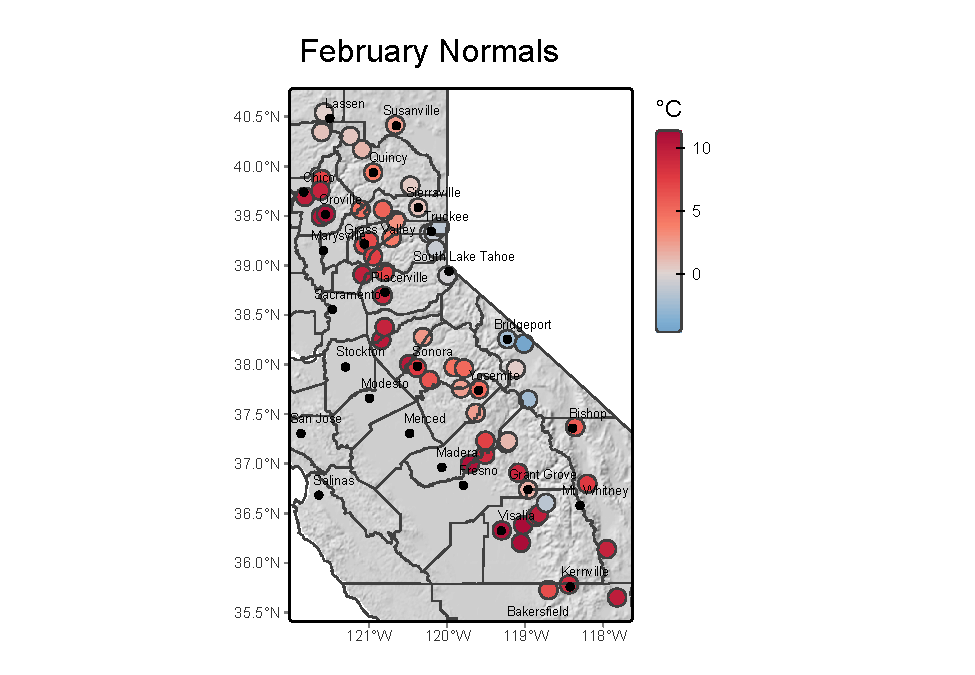
\includegraphics[width=0.9\linewidth]{EnvDataScience_files/figure-latex/modOrigFebTemp-1} 

}

\caption{Original February temperature data}\label{fig:modOrigFebTemp}
\end{figure}

\begin{Shaded}
\begin{Highlighting}[]
\NormalTok{mapBase }\SpecialCharTok{+}
  \FunctionTok{tm\_shape}\NormalTok{(sierra) }\SpecialCharTok{+}
    \FunctionTok{tm\_symbols}\NormalTok{(}\AttributeTok{fill=}\StringTok{"predict"}\NormalTok{, }\AttributeTok{fill.scale=}\NormalTok{tempScale, }\AttributeTok{size=}\FloatTok{0.8}\NormalTok{,}
               \AttributeTok{fill.legend=}\FunctionTok{tm\_legend}\NormalTok{(}\FunctionTok{paste0}\NormalTok{(eqn,}\StringTok{"}\SpecialCharTok{\textbackslash{}n}\StringTok{°C"}\NormalTok{),}\AttributeTok{reverse=}\NormalTok{T,}\AttributeTok{frame=}\NormalTok{F)) }\SpecialCharTok{+}
\NormalTok{  mapTop }\SpecialCharTok{+} \FunctionTok{tm\_title}\NormalTok{(}\StringTok{"February Prediction"}\NormalTok{)}
\end{Highlighting}
\end{Shaded}

\begin{figure}

{\centering 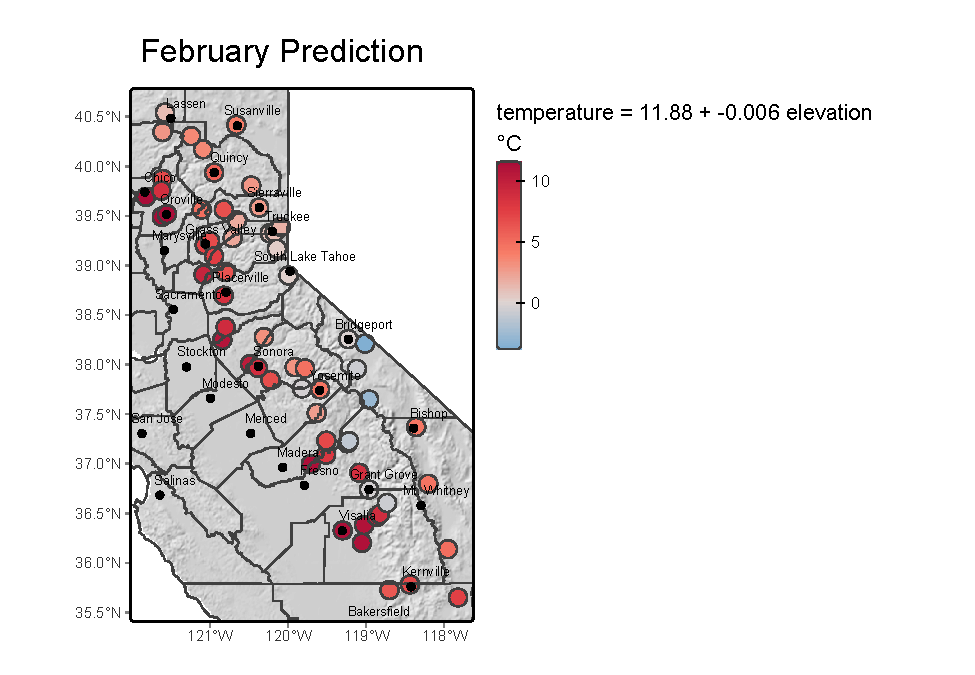
\includegraphics[width=0.9\linewidth]{EnvDataScience_files/figure-latex/modPredictedTemp-1} 

}

\caption{Temperature predicted by elevation model}\label{fig:modPredictedTemp}
\end{figure}

\index{prediction map, model}We can also use the model to predict temperatures from a raster of elevations, which should match the elevations at the weather stations, allowing us to predict temperature for the rest of the study area. We should have more confidence in the area (the Sierra Nevada and nearby areas) actually sampled by the stations, so we'll crop with the extent covering that area (though this will include more coastal areas that are likely to differ in February temperatures from patterns observed in the area sampled).

We'll use GCS elevation raster data and map algebra to derive a prediction raster (Figure \ref{fig:modTempPredRas}). Note that the \texttt{coef()} function is another way to extract the model coefficients.

\begin{Shaded}
\begin{Highlighting}[]
\NormalTok{elev }\OtherTok{\textless{}{-}} \FunctionTok{rast}\NormalTok{(}\FunctionTok{ex}\NormalTok{(}\StringTok{"CA/ca\_elev\_WGS84.tif"}\NormalTok{))}
\NormalTok{elevSierra }\OtherTok{\textless{}{-}} \FunctionTok{crop}\NormalTok{(elev, }\FunctionTok{ext}\NormalTok{(}\SpecialCharTok{{-}}\DecValTok{122}\NormalTok{, }\SpecialCharTok{{-}}\DecValTok{118}\NormalTok{, }\DecValTok{35}\NormalTok{, }\DecValTok{41}\NormalTok{))  }\CommentTok{\# GCS}
\NormalTok{b0 }\OtherTok{\textless{}{-}} \FunctionTok{coef}\NormalTok{(modelElev)[}\DecValTok{1}\NormalTok{]}
\NormalTok{b1 }\OtherTok{\textless{}{-}} \FunctionTok{coef}\NormalTok{(modelElev)[}\DecValTok{2}\NormalTok{]}
\NormalTok{tempSierra }\OtherTok{\textless{}{-}}\NormalTok{ b0 }\SpecialCharTok{+}\NormalTok{ b1 }\SpecialCharTok{*}\NormalTok{ elevSierra}
\FunctionTok{names}\NormalTok{(tempSierra) }\OtherTok{=} \StringTok{"Predicted}\SpecialCharTok{\textbackslash{}n}\StringTok{Temperature"}
\NormalTok{mapBase }\SpecialCharTok{+}
  \FunctionTok{tm\_shape}\NormalTok{(tempSierra) }\SpecialCharTok{+} 
    \FunctionTok{tm\_raster}\NormalTok{(}\AttributeTok{col.scale=}\NormalTok{tempScale,}
              \AttributeTok{col.legend=}\FunctionTok{tm\_legend}\NormalTok{(}\FunctionTok{paste0}\NormalTok{(eqn,}\StringTok{"}\SpecialCharTok{\textbackslash{}n}\StringTok{°C"}\NormalTok{),}\AttributeTok{reverse=}\NormalTok{T,}\AttributeTok{frame=}\NormalTok{F)) }\SpecialCharTok{+}
\NormalTok{  mapTop }\SpecialCharTok{+} \FunctionTok{tm\_title}\NormalTok{(}\StringTok{"February Prediction"}\NormalTok{)}
\end{Highlighting}
\end{Shaded}

\begin{figure}

{\centering 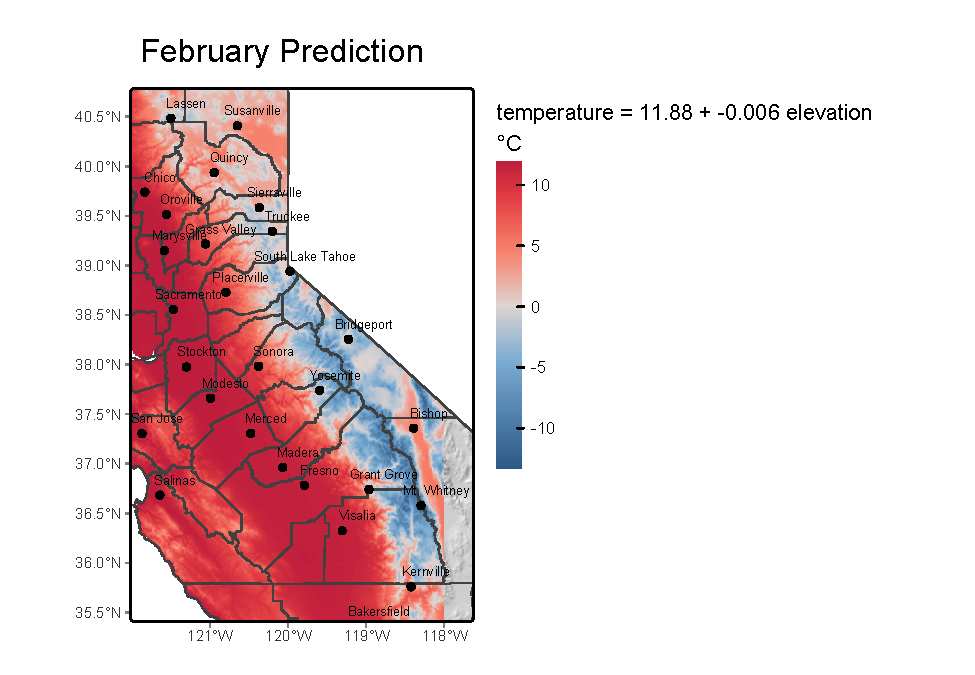
\includegraphics[width=0.9\linewidth]{EnvDataScience_files/figure-latex/modTempPredRas-1} 

}

\caption{Temperature predicted by elevation raster}\label{fig:modTempPredRas}
\end{figure}

\textbf{The residuals}

\index{residuals, mapping}To consider patterns where the simple elevation model \emph{doesn't} work well, we can map the model residuals at the stations (Figure \ref{fig:modResidualsTemp}).

\begin{Shaded}
\begin{Highlighting}[]
\NormalTok{mapBase }\SpecialCharTok{+} 
  \FunctionTok{tm\_shape}\NormalTok{(sierra) }\SpecialCharTok{+}
    \FunctionTok{tm\_symbols}\NormalTok{(}\AttributeTok{fill=}\StringTok{"resid"}\NormalTok{, }\AttributeTok{fill.scale=}\NormalTok{tempScale, }\AttributeTok{size=}\FloatTok{0.8}\NormalTok{,}
               \AttributeTok{fill.legend=}\FunctionTok{tm\_legend}\NormalTok{(}\StringTok{"°C"}\NormalTok{, }\AttributeTok{reverse=}\NormalTok{T,}\AttributeTok{frame=}\NormalTok{F)) }\SpecialCharTok{+}
\NormalTok{  mapTop }\SpecialCharTok{+} \FunctionTok{tm\_title}\NormalTok{(}\StringTok{"February residuals"}\NormalTok{)}
\end{Highlighting}
\end{Shaded}

\begin{figure}

{\centering 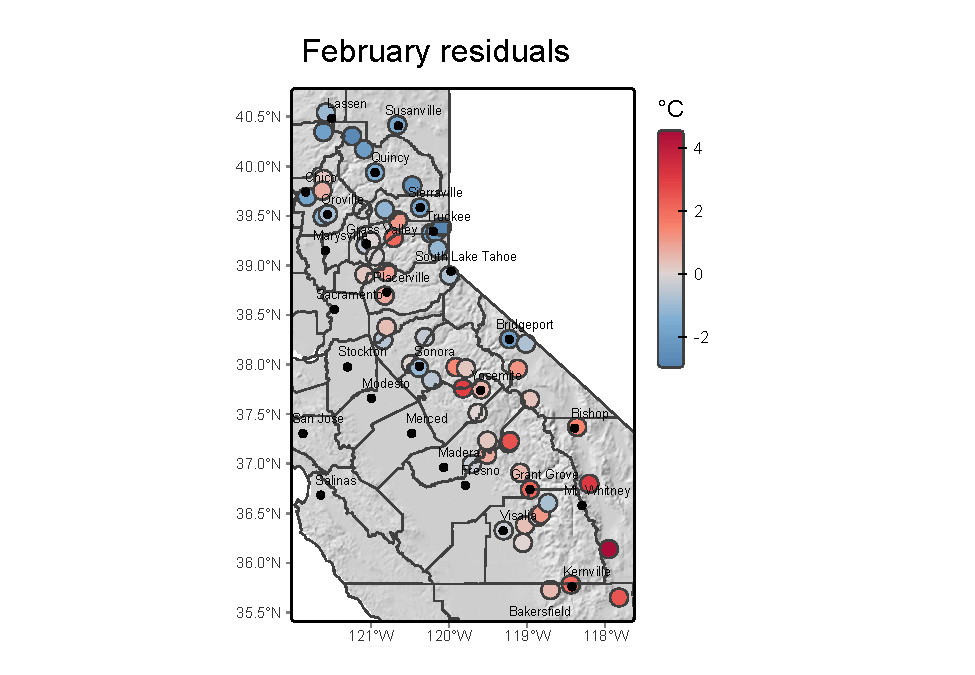
\includegraphics[width=0.9\linewidth]{EnvDataScience_files/figure-latex/modResidualsTemp-1} 

}

\caption{Residuals of temperature from model predictions by elevation}\label{fig:modResidualsTemp}
\end{figure}

Statistically, if the \emph{residuals} from regression are spatially autocorrelated, we should look for patterns in the residuals to find other explanatory variables. However, we can visually see, based upon the pattern of the residuals, that there's at least one important explanatory variable not included in the model: latitude. We'll leave that for you to look at in the exercises.

\section{Analysis of Covariance}\label{analysis-of-covariance}

\index{analysis of covariance}\index{ANCOVA}Analysis of covariance, or ANCOVA, has the same purpose as ANOVA that we looked at under tests earlier, but also takes into account the influence of other variables called covariates. In this way, analysis of covariance combines a linear model with an analysis of variance.

\emph{``Are water samples from streams draining sandstone, limestone, and shale different based on carbonate solutes, while taking into account elevation?''}

The response variable\index{response variable} is modeled from the factor (ANOVA) plus the covariate\index{covariate} (regression):

\begin{itemize}
\item
  ANOVA: \texttt{TH\ \textasciitilde{}\ lithology} where \texttt{TH} is total hardness, a measure of carbonate solutes
\item
  Regression: \texttt{TH\ \textasciitilde{}\ elevation}
\item
  ANCOVA: \texttt{TH\ \textasciitilde{}\ lithology\ +\ elevation}

  \begin{itemize}
  \tightlist
  \item
    Yet shouldn't involve interaction between \texttt{lithology} (factor) and \texttt{elevation} (covariate):
  \end{itemize}
\end{itemize}

However, as we'll see in a bit, this particular problem doesn't lend itself to ANCOVA because there's in fact a lot of interaction between lithology and elevation, because the Cumberland Plateau has essentially horizontal geologic structure, so all of the sandstone caprock is at the highest elevation. So we'll look at a better example.

\textbf{Example: stream types distinguished by discharge and slope}

Before we look at that water chemistry model predicted by lithology while taking elevation into consideration, we'll look at a clearer example of the use of ANCOVA, distinguishing stream types on the basis of discharge and slope.

\index{rivers, ANCOVA}Three common river types are meandering (Figure \ref{fig:modMeandering}), braided (Figure \ref{fig:modBraided}), and anastomosed (Figure \ref{fig:modAnastomosed}).

\begin{figure}

{\centering 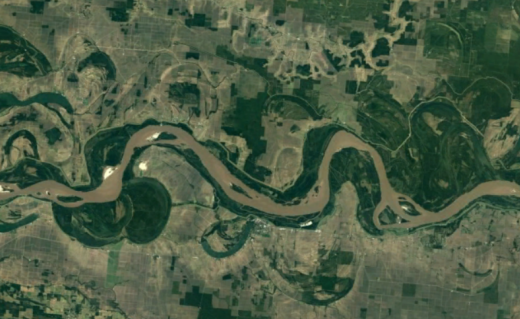
\includegraphics[width=0.75\linewidth]{img/meanderingRiver} 

}

\caption{Meandering river}\label{fig:modMeandering}
\end{figure}

\begin{figure}

{\centering 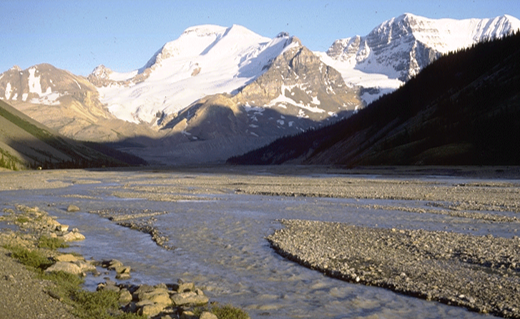
\includegraphics[width=0.75\linewidth]{img/braided} 

}

\caption{Braided river}\label{fig:modBraided}
\end{figure}

\begin{figure}

{\centering 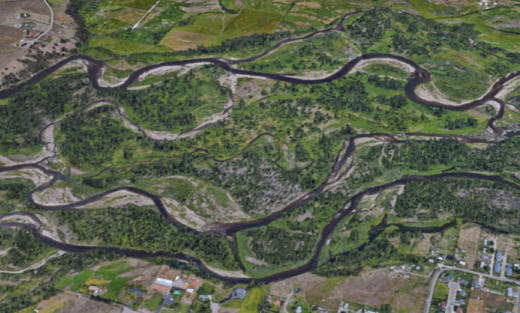
\includegraphics[width=0.75\linewidth]{img/anastomosed} 

}

\caption{Anastomosed river}\label{fig:modAnastomosed}
\end{figure}

For each, their slope varies by bankfull discharge in a relationship that looks something like Figure \ref{fig:modQSrivers}, which employs a log10 scale on both axes:

\begin{Shaded}
\begin{Highlighting}[]
\FunctionTok{library}\NormalTok{(tidyverse)}
\NormalTok{csvPath }\OtherTok{\textless{}{-}} \FunctionTok{system.file}\NormalTok{(}\StringTok{"extdata"}\NormalTok{,}\StringTok{"streams.csv"}\NormalTok{, }\AttributeTok{package=}\StringTok{"igisci"}\NormalTok{)}
\NormalTok{streams }\OtherTok{\textless{}{-}} \FunctionTok{read\_csv}\NormalTok{(csvPath)}
\NormalTok{streams}\SpecialCharTok{$}\NormalTok{strtype }\OtherTok{\textless{}{-}} \FunctionTok{factor}\NormalTok{(streams}\SpecialCharTok{$}\NormalTok{type, }
                          \AttributeTok{labels=}\FunctionTok{c}\NormalTok{(}\StringTok{"Anastomosing"}\NormalTok{,}\StringTok{"Braided"}\NormalTok{,}\StringTok{"Meandering"}\NormalTok{))}
\FunctionTok{library}\NormalTok{(scales) }\CommentTok{\# needed for the trans\_format function below}
\FunctionTok{ggplot}\NormalTok{(streams, }\FunctionTok{aes}\NormalTok{(Q, S, }\AttributeTok{color=}\NormalTok{strtype)) }\SpecialCharTok{+}
  \FunctionTok{geom\_point}\NormalTok{() }\SpecialCharTok{+} \FunctionTok{geom\_smooth}\NormalTok{(}\AttributeTok{method=}\StringTok{"lm"}\NormalTok{, }\AttributeTok{se =} \ConstantTok{FALSE}\NormalTok{) }\SpecialCharTok{+} 
  \FunctionTok{scale\_x\_continuous}\NormalTok{(}\AttributeTok{trans=}\FunctionTok{log10\_trans}\NormalTok{(),}
                     \AttributeTok{labels =} \FunctionTok{trans\_format}\NormalTok{(}\StringTok{"log10"}\NormalTok{, }\FunctionTok{math\_format}\NormalTok{(}\DecValTok{10}\SpecialCharTok{\^{}}\NormalTok{.x))) }\SpecialCharTok{+}
  \FunctionTok{scale\_y\_continuous}\NormalTok{(}\AttributeTok{trans=}\FunctionTok{log10\_trans}\NormalTok{(),}
                     \AttributeTok{labels =} \FunctionTok{trans\_format}\NormalTok{(}\StringTok{"log10"}\NormalTok{, }\FunctionTok{math\_format}\NormalTok{(}\DecValTok{10}\SpecialCharTok{\^{}}\NormalTok{.x)))}
\end{Highlighting}
\end{Shaded}

\begin{figure}

{\centering 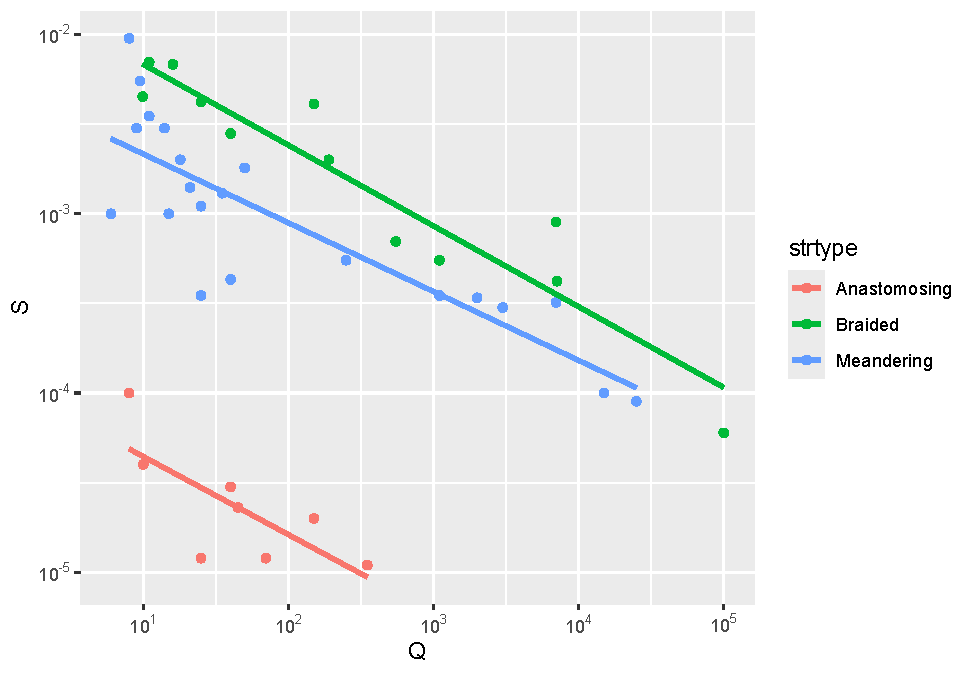
\includegraphics[width=0.75\linewidth]{EnvDataScience_files/figure-latex/modQSrivers-1} 

}

\caption{Q vs S with stream type}\label{fig:modQSrivers}
\end{figure}

One requirement for the ANCOVA model\index{ANCOVA requirements} is that there's no relationship between discharge (covariate) and channel type (factor). Another way of thinking about this is that the slope of the relationship between the covariate and response variable needs to be about the same for each group; only the intercept differs. One good way to understand this is we're just adjusting the response variable by the group means of the covariate, which results in a simple adjustment the y intercept. The groups have reasonably parallel slopes in the graph, at least for log-transformed data, so that's looking good. Here are two model definitions in R and what they mean for the analysis:

\texttt{log10(S)\ \textasciitilde{}\ strtype\ *\ log10(Q)} \ldots{} interaction between covariate and factor

\texttt{log10(S)\ \textasciitilde{}\ strtype\ +\ log10(Q)} \ldots{} no interaction, parallel slopes

In the ANCOVA process, if these models are not significantly different, we can remove the interaction term due to parsimony, and thus satisfy this ANCOVA requirement. So we can go through the process:

\begin{Shaded}
\begin{Highlighting}[]
\NormalTok{ancova }\OtherTok{=} \FunctionTok{lm}\NormalTok{(}\FunctionTok{log10}\NormalTok{(S)}\SpecialCharTok{\textasciitilde{}}\NormalTok{strtype}\SpecialCharTok{*}\FunctionTok{log10}\NormalTok{(Q), }\AttributeTok{data=}\NormalTok{streams)}
\FunctionTok{anova}\NormalTok{(ancova)}
\end{Highlighting}
\end{Shaded}

\begin{verbatim}
## Analysis of Variance Table
## 
## Response: log10(S)
##                  Df  Sum Sq Mean Sq  F value    Pr(>F)    
## strtype           2 18.3914  9.1957 130.3650 < 2.2e-16 ***
## log10(Q)          1  8.2658  8.2658 117.1821 1.023e-12 ***
## strtype:log10(Q)  2  0.0511  0.0255   0.3619    0.6989    
## Residuals        35  2.4688  0.0705                       
## ---
## Signif. codes:  0 '***' 0.001 '**' 0.01 '*' 0.05 '.' 0.1 ' ' 1
\end{verbatim}

\textbf{Now an additive model, which does not have that interaction:}

\begin{Shaded}
\begin{Highlighting}[]
\NormalTok{ancova2 }\OtherTok{=} \FunctionTok{lm}\NormalTok{(}\FunctionTok{log10}\NormalTok{(S)}\SpecialCharTok{\textasciitilde{}}\NormalTok{strtype}\SpecialCharTok{+}\FunctionTok{log10}\NormalTok{(Q), }\AttributeTok{data=}\NormalTok{streams)}
\FunctionTok{anova}\NormalTok{(ancova2)}
\end{Highlighting}
\end{Shaded}

\begin{verbatim}
## Analysis of Variance Table
## 
## Response: log10(S)
##           Df  Sum Sq Mean Sq F value    Pr(>F)    
## strtype    2 18.3914  9.1957  135.02 < 2.2e-16 ***
## log10(Q)   1  8.2658  8.2658  121.37  3.07e-13 ***
## Residuals 37  2.5199  0.0681                      
## ---
## Signif. codes:  0 '***' 0.001 '**' 0.01 '*' 0.05 '.' 0.1 ' ' 1
\end{verbatim}

\textbf{Now see if the two models are significantly different:}

\begin{Shaded}
\begin{Highlighting}[]
\FunctionTok{anova}\NormalTok{(ancova,ancova2) }\CommentTok{\# not significantly different, so simplification is justified}
\end{Highlighting}
\end{Shaded}

\begin{verbatim}
## Analysis of Variance Table
## 
## Model 1: log10(S) ~ strtype * log10(Q)
## Model 2: log10(S) ~ strtype + log10(Q)
##   Res.Df    RSS Df Sum of Sq      F Pr(>F)
## 1     35 2.4688                           
## 2     37 2.5199 -2 -0.051051 0.3619 0.6989
\end{verbatim}

\emph{They're not significantly different, so simplification is justified and appropriate in the interest of parsimony.}

\textbf{Now we'll go one step further and remove the strtype term, which is just a simple regression:}

\begin{Shaded}
\begin{Highlighting}[]
\NormalTok{SQlm }\OtherTok{=} \FunctionTok{lm}\NormalTok{(}\FunctionTok{log10}\NormalTok{(S)}\SpecialCharTok{\textasciitilde{}}\FunctionTok{log10}\NormalTok{(Q), }\AttributeTok{data=}\NormalTok{streams)}
\FunctionTok{anova}\NormalTok{(SQlm)}
\end{Highlighting}
\end{Shaded}

\begin{verbatim}
## Analysis of Variance Table
## 
## Response: log10(S)
##           Df  Sum Sq Mean Sq F value  Pr(>F)  
## log10(Q)   1  3.6671  3.6671  5.6063 0.02295 *
## Residuals 39 25.5099  0.6541                  
## ---
## Signif. codes:  0 '***' 0.001 '**' 0.01 '*' 0.05 '.' 0.1 ' ' 1
\end{verbatim}

\textbf{Is the ANCOVA model significantly different from a simple linear model with no factor?}

\begin{Shaded}
\begin{Highlighting}[]
\FunctionTok{anova}\NormalTok{(ancova2,SQlm)  }\CommentTok{\# Goes too far: removing strtype significantly different}
\end{Highlighting}
\end{Shaded}

\begin{verbatim}
## Analysis of Variance Table
## 
## Model 1: log10(S) ~ strtype + log10(Q)
## Model 2: log10(S) ~ log10(Q)
##   Res.Df     RSS Df Sum of Sq      F    Pr(>F)    
## 1     37  2.5199                                  
## 2     39 25.5099 -2    -22.99 168.78 < 2.2e-16 ***
## ---
## Signif. codes:  0 '***' 0.001 '**' 0.01 '*' 0.05 '.' 0.1 ' ' 1
\end{verbatim}

\emph{Since removing the strtype produces a significantly different model, we've gone too far, so the strtype groupings mean something; the responses just have different means.}

\begin{quote}
You should have noticed above a surprising use of \texttt{anova()} to compare two models to see if they're different. As with other functions in R, it's always useful to use the help system, so you'll see with \texttt{?anova} that it has these two ways of working: as a summary for a single input model, and as a comparison when provided with multiple models.
\end{quote}

Alternatively, we can use R's step method for a more automated approach.

\begin{Shaded}
\begin{Highlighting}[]
\NormalTok{ancova }\OtherTok{=} \FunctionTok{lm}\NormalTok{(}\FunctionTok{log10}\NormalTok{(S)}\SpecialCharTok{\textasciitilde{}}\NormalTok{strtype}\SpecialCharTok{*}\FunctionTok{log10}\NormalTok{(Q), }\AttributeTok{data=}\NormalTok{streams)}
\FunctionTok{step}\NormalTok{(ancova)}
\end{Highlighting}
\end{Shaded}

\begin{verbatim}
## Start:  AIC=-103.2
## log10(S) ~ strtype * log10(Q)
## 
##                    Df Sum of Sq    RSS     AIC
## - strtype:log10(Q)  2  0.051051 2.5199 -106.36
## <none>                          2.4688 -103.20
## 
## Step:  AIC=-106.36
## log10(S) ~ strtype + log10(Q)
## 
##            Df Sum of Sq     RSS      AIC
## <none>                   2.5199 -106.364
## - log10(Q)  1    8.2658 10.7857  -48.750
## - strtype   2   22.9901 25.5099  -15.455
\end{verbatim}

\begin{verbatim}
## 
## Call:
## lm(formula = log10(S) ~ strtype + log10(Q), data = streams)
## 
## Coefficients:
##       (Intercept)     strtypeBraided  strtypeMeandering           log10(Q)  
##           -3.9583             2.1453             1.7294            -0.4109
\end{verbatim}

ANOVA and ANCOVA are applications of a linear model\index{ANOVA and ANCOVA as lm}. They use the \texttt{lm} model and the response variable is continuous and assumed normally distributed. The linear model for the stream types employing slope (S) and the covariate discharge (log\textsubscript{10}Q) was produced using:

\texttt{mymodel\ \textless{}-\ lm(log10(S)\ \textasciitilde{}\ strtype\ +\ log10(Q))}

Then as with standard ANOVA, we displayed the results using:

\texttt{anova(mymodel)}

\subsection{Tukey test for the ANCOVA model}\label{tukey-test-for-the-ancova-model}

As we did with ANOVA in the last chapter, we can do a bit of post-hoc analysis with TukeyHSD. One minor difference with analysis of covariance is that you need to specify which variable you're analyzing by using the \texttt{which} parameter to specify the factor \texttt{strtype}. Also, we need to use \texttt{aov()} instead of \texttt{lm()}, even though functionally they're the same.

\begin{Shaded}
\begin{Highlighting}[]
\NormalTok{mymodel }\OtherTok{\textless{}{-}} \FunctionTok{aov}\NormalTok{(}\FunctionTok{log10}\NormalTok{(S) }\SpecialCharTok{\textasciitilde{}}\NormalTok{ strtype }\SpecialCharTok{+} \FunctionTok{log10}\NormalTok{(Q), }\AttributeTok{data=}\NormalTok{streams)}
\FunctionTok{TukeyHSD}\NormalTok{(mymodel, }\AttributeTok{conf.level=}\NormalTok{.}\DecValTok{95}\NormalTok{, }\AttributeTok{which=}\StringTok{\textquotesingle{}strtype\textquotesingle{}}\NormalTok{)}
\end{Highlighting}
\end{Shaded}

\begin{verbatim}
##   Tukey multiple comparisons of means
##     95% family-wise confidence level
## 
## Fit: aov(formula = log10(S) ~ strtype + log10(Q), data = streams)
## 
## $strtype
##                               diff        lwr          upr     p adj
## Braided-Anastomosing     1.8203003  1.5294814  2.111119063 0.0000000
## Meandering-Anastomosing  1.5848655  1.3201451  1.849585955 0.0000000
## Meandering-Braided      -0.2354347 -0.4660031 -0.004866321 0.0444972
\end{verbatim}

With this, we can be more confident in saying that all of the pairings are significantly distinct.

\subsection{The karst water chemistry model}\label{the-karst-water-chemistry-model}

We started off this section presenting the question: \emph{``Are water samples from streams draining sandstone, limestone, and shale different based on carbonate solutes, while taking into account elevation?''} So let's look at that.

We'll start by reviewing what we saw with the ANOVA test in the last chapter where we prepared the data to consider whether dissolved carbonates (measured as total hardness (TH)) was predicted by lithology.

\begin{Shaded}
\begin{Highlighting}[]
\FunctionTok{library}\NormalTok{(igisci)}
\FunctionTok{library}\NormalTok{(sf); }\FunctionTok{library}\NormalTok{(tidyverse); }\FunctionTok{library}\NormalTok{(readxl); }\FunctionTok{library}\NormalTok{(tmap); }\FunctionTok{library}\NormalTok{(terra)}
\NormalTok{wChemData }\OtherTok{\textless{}{-}} \FunctionTok{read\_excel}\NormalTok{(}\FunctionTok{ex}\NormalTok{(}\StringTok{"SinkingCove/SinkingCoveWaterChem.xlsx"}\NormalTok{)) }\SpecialCharTok{\%\textgreater{}\%}
  \FunctionTok{mutate}\NormalTok{(}\AttributeTok{siteLoc =} \FunctionTok{str\_sub}\NormalTok{(Site,}\AttributeTok{start=}\DecValTok{1}\DataTypeTok{L}\NormalTok{, }\AttributeTok{end=}\DecValTok{1}\DataTypeTok{L}\NormalTok{))}
\NormalTok{wChemTrunk }\OtherTok{\textless{}{-}}\NormalTok{ wChemData }\SpecialCharTok{\%\textgreater{}\%} \FunctionTok{filter}\NormalTok{(siteLoc }\SpecialCharTok{==} \StringTok{"T"}\NormalTok{) }\SpecialCharTok{\%\textgreater{}\%} \FunctionTok{mutate}\NormalTok{(}\AttributeTok{siteType =} \StringTok{"trunk"}\NormalTok{)}
\NormalTok{wChemDrip }\OtherTok{\textless{}{-}}\NormalTok{ wChemData }\SpecialCharTok{\%\textgreater{}\%} \FunctionTok{filter}\NormalTok{(siteLoc }\SpecialCharTok{\%in\%} \FunctionTok{c}\NormalTok{(}\StringTok{"D"}\NormalTok{,}\StringTok{"S"}\NormalTok{)) }\SpecialCharTok{\%\textgreater{}\%} \FunctionTok{mutate}\NormalTok{(}\AttributeTok{siteType =} \StringTok{"dripwater"}\NormalTok{)}
\NormalTok{wChemTrib }\OtherTok{\textless{}{-}}\NormalTok{ wChemData }\SpecialCharTok{\%\textgreater{}\%} \FunctionTok{filter}\NormalTok{(siteLoc }\SpecialCharTok{\%in\%} \FunctionTok{c}\NormalTok{(}\StringTok{"B"}\NormalTok{, }\StringTok{"F"}\NormalTok{, }\StringTok{"K"}\NormalTok{, }\StringTok{"W"}\NormalTok{, }\StringTok{"P"}\NormalTok{)) }\SpecialCharTok{\%\textgreater{}\%} 
  \FunctionTok{mutate}\NormalTok{(}\AttributeTok{siteType =} \StringTok{"tributary"}\NormalTok{)}
\NormalTok{wChemData }\OtherTok{\textless{}{-}} \FunctionTok{bind\_rows}\NormalTok{(wChemTrunk, wChemDrip, wChemTrib)}
\NormalTok{wChemData}\SpecialCharTok{$}\NormalTok{siteType }\OtherTok{\textless{}{-}} \FunctionTok{factor}\NormalTok{(wChemData}\SpecialCharTok{$}\NormalTok{siteType)}
\NormalTok{wChemData}\SpecialCharTok{$}\NormalTok{Lithology }\OtherTok{\textless{}{-}} \FunctionTok{factor}\NormalTok{(wChemData}\SpecialCharTok{$}\NormalTok{Lithology)}
\NormalTok{sites }\OtherTok{\textless{}{-}} \FunctionTok{read\_csv}\NormalTok{(}\FunctionTok{ex}\NormalTok{(}\StringTok{"SinkingCove/SinkingCoveSites.csv"}\NormalTok{))}
\NormalTok{wChem }\OtherTok{\textless{}{-}}\NormalTok{ wChemData }\SpecialCharTok{\%\textgreater{}\%}
  \FunctionTok{left\_join}\NormalTok{(sites, }\AttributeTok{by =} \FunctionTok{c}\NormalTok{(}\StringTok{"Site"} \OtherTok{=} \StringTok{"site"}\NormalTok{)) }\SpecialCharTok{\%\textgreater{}\%}
  \FunctionTok{st\_as\_sf}\NormalTok{(}\AttributeTok{coords =} \FunctionTok{c}\NormalTok{(}\StringTok{"longitude"}\NormalTok{, }\StringTok{"latitude"}\NormalTok{), }\AttributeTok{crs =} \DecValTok{4326}\NormalTok{)}
\end{Highlighting}
\end{Shaded}

\textbf{Plotting the relationship to see if ANCOVA might work}
With ANCOVA we're seeing if a covariate (in this case elevation) plays a role in influencing the effect of lithology on TH. We're looking for parallel relationships between groups defined by rock types. Do we have that?

\begin{Shaded}
\begin{Highlighting}[]
\FunctionTok{library}\NormalTok{(scales)}
\FunctionTok{ggplot}\NormalTok{(wChemData, }\FunctionTok{aes}\NormalTok{(Elevation,TH,}\AttributeTok{col=}\NormalTok{Lithology)) }\SpecialCharTok{+}
  \FunctionTok{geom\_point}\NormalTok{() }\SpecialCharTok{+} \FunctionTok{geom\_smooth}\NormalTok{(}\AttributeTok{method=}\StringTok{"lm"}\NormalTok{, }\AttributeTok{se=}\NormalTok{F) }\SpecialCharTok{+}
  \FunctionTok{scale\_x\_continuous}\NormalTok{(}\AttributeTok{trans=}\FunctionTok{log10\_trans}\NormalTok{(),}
                     \AttributeTok{labels =} \FunctionTok{trans\_format}\NormalTok{(}\StringTok{"log10"}\NormalTok{, }\FunctionTok{math\_format}\NormalTok{(}\DecValTok{10}\SpecialCharTok{\^{}}\NormalTok{.x))) }\SpecialCharTok{+}
  \FunctionTok{scale\_y\_continuous}\NormalTok{(}\AttributeTok{trans=}\FunctionTok{log10\_trans}\NormalTok{(),}
                     \AttributeTok{labels =} \FunctionTok{trans\_format}\NormalTok{(}\StringTok{"log10"}\NormalTok{, }\FunctionTok{math\_format}\NormalTok{(}\DecValTok{10}\SpecialCharTok{\^{}}\NormalTok{.x)))}
\end{Highlighting}
\end{Shaded}

\begin{center}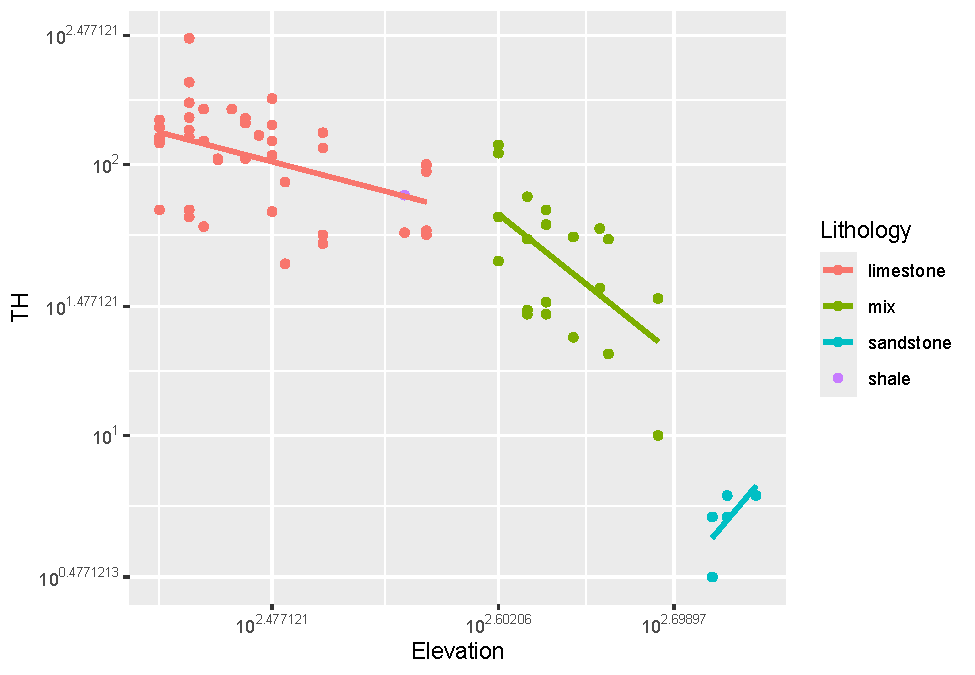
\includegraphics[width=0.75\linewidth]{EnvDataScience_files/figure-latex/unnamed-chunk-290-1} \end{center}

Right off the bat, we see a problem -- the samples are at very different elevations. This isn't surprising since geologic structure is nearly horizontal, with a sandstone caprock of the Cumberland Plateau meaning that any water samples from sandstone are from the maximum elevations. But let's see what happens with the same ANCOVA process.

\textbf{Starting with the interactive model we'll call ancova}:

\begin{Shaded}
\begin{Highlighting}[]
\NormalTok{ancova }\OtherTok{=} \FunctionTok{lm}\NormalTok{(}\FunctionTok{log10}\NormalTok{(TH)}\SpecialCharTok{\textasciitilde{}}\NormalTok{Lithology}\SpecialCharTok{*}\FunctionTok{log10}\NormalTok{(Elevation), }\AttributeTok{data=}\NormalTok{wChemData)}
\FunctionTok{summary}\NormalTok{(ancova)}
\end{Highlighting}
\end{Shaded}

\begin{verbatim}
## 
## Call:
## lm(formula = log10(TH) ~ Lithology * log10(Elevation), data = wChemData)
## 
## Residuals:
##      Min       1Q   Median       3Q      Max 
## -0.36415 -0.13110  0.01507  0.13443  0.37541 
## 
## Coefficients: (1 not defined because of singularities)
##                                       Estimate Std. Error t value Pr(>|t|)    
## (Intercept)                           6.331769   1.467184   4.316 5.73e-05 ***
## Lithologymix                          9.361794   4.144554   2.259  0.02736 *  
## Lithologysandstone                  -27.245212  24.972709  -1.091  0.27943    
## Lithologyshale                        0.003894   0.188754   0.021  0.98361    
## log10(Elevation)                     -1.744617   0.594632  -2.934  0.00466 ** 
## Lithologymix:log10(Elevation)        -3.588442   1.585964  -2.263  0.02712 *  
## Lithologysandstone:log10(Elevation)   9.661636   9.156802   1.055  0.29539    
## Lithologyshale:log10(Elevation)             NA         NA      NA       NA    
## ---
## Signif. codes:  0 '***' 0.001 '**' 0.01 '*' 0.05 '.' 0.1 ' ' 1
## 
## Residual standard error: 0.1801 on 63 degrees of freedom
## Multiple R-squared:  0.8266, Adjusted R-squared:  0.8101 
## F-statistic: 50.06 on 6 and 63 DF,  p-value: < 2.2e-16
\end{verbatim}

\begin{Shaded}
\begin{Highlighting}[]
\FunctionTok{anova}\NormalTok{(ancova)}
\end{Highlighting}
\end{Shaded}

\begin{verbatim}
## Analysis of Variance Table
## 
## Response: log10(TH)
##                            Df Sum Sq Mean Sq F value    Pr(>F)    
## Lithology                   3 9.0084 3.00281 92.6167 < 2.2e-16 ***
## log10(Elevation)            1 0.5240 0.52403 16.1630 0.0001579 ***
## Lithology:log10(Elevation)  2 0.2060 0.10298  3.1764 0.0484967 *  
## Residuals                  63 2.0426 0.03242                      
## ---
## Signif. codes:  0 '***' 0.001 '**' 0.01 '*' 0.05 '.' 0.1 ' ' 1
\end{verbatim}

\textbf{Now an additive model, which does not have that interaction}:

\begin{Shaded}
\begin{Highlighting}[]
\NormalTok{ancova2 }\OtherTok{=} \FunctionTok{lm}\NormalTok{(}\FunctionTok{log10}\NormalTok{(TH)}\SpecialCharTok{\textasciitilde{}}\NormalTok{Lithology}\SpecialCharTok{+}\FunctionTok{log10}\NormalTok{(Elevation), }\AttributeTok{data=}\NormalTok{wChemData)}
\FunctionTok{anova}\NormalTok{(ancova2)}
\end{Highlighting}
\end{Shaded}

\begin{verbatim}
## Analysis of Variance Table
## 
## Response: log10(TH)
##                  Df Sum Sq Mean Sq F value    Pr(>F)    
## Lithology         3 9.0084 3.00281  86.804 < 2.2e-16 ***
## log10(Elevation)  1 0.5240 0.52403  15.149 0.0002367 ***
## Residuals        65 2.2485 0.03459                      
## ---
## Signif. codes:  0 '***' 0.001 '**' 0.01 '*' 0.05 '.' 0.1 ' ' 1
\end{verbatim}

\begin{Shaded}
\begin{Highlighting}[]
\FunctionTok{anova}\NormalTok{(ancova,ancova2)}
\end{Highlighting}
\end{Shaded}

\begin{verbatim}
## Analysis of Variance Table
## 
## Model 1: log10(TH) ~ Lithology * log10(Elevation)
## Model 2: log10(TH) ~ Lithology + log10(Elevation)
##   Res.Df    RSS Df Sum of Sq      F Pr(>F)  
## 1     63 2.0426                             
## 2     65 2.2485 -2  -0.20597 3.1764 0.0485 *
## ---
## Signif. codes:  0 '***' 0.001 '**' 0.01 '*' 0.05 '.' 0.1 ' ' 1
\end{verbatim}

The fairly low (less than 0.05) p value means the models are significantly different, so we need to stick with the interaction model. Elevation interacts with lithology due to the horizontal structure. A stepwise approach shows the same thing:

\begin{Shaded}
\begin{Highlighting}[]
\NormalTok{ancova }\OtherTok{=} \FunctionTok{lm}\NormalTok{(}\FunctionTok{log10}\NormalTok{(TH)}\SpecialCharTok{\textasciitilde{}}\NormalTok{Lithology}\SpecialCharTok{*}\FunctionTok{log10}\NormalTok{(Elevation), }\AttributeTok{data=}\NormalTok{wChemData)}
\FunctionTok{step}\NormalTok{(ancova)}
\end{Highlighting}
\end{Shaded}

\begin{verbatim}
## Start:  AIC=-233.4
## log10(TH) ~ Lithology * log10(Elevation)
## 
##                              Df Sum of Sq    RSS     AIC
## <none>                                    2.0426 -233.40
## - Lithology:log10(Elevation)  2   0.20597 2.2485 -230.68
\end{verbatim}

\begin{verbatim}
## 
## Call:
## lm(formula = log10(TH) ~ Lithology * log10(Elevation), data = wChemData)
## 
## Coefficients:
##                         (Intercept)                         Lithologymix  
##                            6.331769                             9.361794  
##                  Lithologysandstone                       Lithologyshale  
##                          -27.245212                             0.003894  
##                    log10(Elevation)        Lithologymix:log10(Elevation)  
##                           -1.744617                            -3.588442  
## Lithologysandstone:log10(Elevation)      Lithologyshale:log10(Elevation)  
##                            9.661636                                   NA
\end{verbatim}

So this isn't something we can apply ANCOVA to, \emph{but it's not surprising}.

\section{Generalized linear model (GLM)}\label{generalized-linear-model-glm}

The glm\index{glm}\index{generalized linear model glm} in R allows you to work with various types of data using various distributions, described as families such as:

\begin{itemize}
\item
  \texttt{gaussian} : normal distribution -- what is used with lm
\item
  \texttt{binomial} : \index{binomial}logit\index{logit} -- used with probabilities\index{probabilities (for logit)}

  \begin{itemize}
  \tightlist
  \item
    used for \emph{logistic regression}
  \end{itemize}
\item
  \texttt{poisson} : \index{poisson}for counts -- commonly used for species counts\index{species counts}
\end{itemize}

See \texttt{help(glm)} for other examples

\subsection{Binomial family: Logistic GLM}\label{binomial-family-logistic-glm}

We'll look at a couple of examples from data we've used before: Eucs vs oaks and stream types.

In both cases, we'll create \emph{dummy variables} to handle categorical variables as continuous. Dummy variables simply have the value 1 or 0 representing whether a particular category is true or false, e.g.~is the sample from a Eucalyptus grove or not. This is frequently used in linear modeling for predictor variables, but we're going to use them for a response variable. With the binomial glm family, this is called \emph{logistic regression}\index{logistic regression}, where we're predicting the \emph{probability} of something being true, though our input response data only has 0\% or 100\% values.

In the case of eucs vs.~oaks, we only have two categories, so choosing either one works the same -- if the sample is euc, it's not oak, and vice-versa. We'll create a variable \texttt{euc} to represent whether it's Eucalyptus or not.

\begin{Shaded}
\begin{Highlighting}[]
\NormalTok{eucoak }\OtherTok{\textless{}{-}}\NormalTok{ tidy\_eucoak }\SpecialCharTok{|\textgreater{}}
  \FunctionTok{mutate}\NormalTok{(}\AttributeTok{euc =}\NormalTok{ (tree}\SpecialCharTok{==}\StringTok{"euc"}\NormalTok{)}\SpecialCharTok{*}\DecValTok{1}\NormalTok{)}
\NormalTok{runoff\_model }\OtherTok{\textless{}{-}} \FunctionTok{glm}\NormalTok{(euc }\SpecialCharTok{\textasciitilde{}}\NormalTok{ rain\_subcanopy }\SpecialCharTok{+}\NormalTok{ slope }\SpecialCharTok{+}\NormalTok{ aspect }\SpecialCharTok{+}
\NormalTok{                          surface\_tension }\SpecialCharTok{+}\NormalTok{ runoff\_L }\SpecialCharTok{+}\NormalTok{ runoff\_rainfall\_ratio, }
                    \AttributeTok{family=}\NormalTok{binomial, }
                    \AttributeTok{data=}\NormalTok{eucoak)}
\FunctionTok{summary}\NormalTok{(runoff\_model)}
\end{Highlighting}
\end{Shaded}

\begin{verbatim}
## 
## Call:
## glm(formula = euc ~ rain_subcanopy + slope + aspect + surface_tension + 
##     runoff_L + runoff_rainfall_ratio, family = binomial, data = eucoak)
## 
## Coefficients:
##                         Estimate Std. Error z value Pr(>|z|)    
## (Intercept)            6.656e+00  1.730e+00   3.848 0.000119 ***
## rain_subcanopy         3.165e-03  1.387e-02   0.228 0.819491    
## slope                 -2.546e-02  3.269e-02  -0.779 0.436059    
## aspect                -5.799e-06  4.888e-03  -0.001 0.999053    
## surface_tension       -1.108e-01  1.754e-02  -6.316 2.68e-10 ***
## runoff_L               1.181e-01  1.892e-01   0.624 0.532520    
## runoff_rainfall_ratio -2.158e+00  7.212e+00  -0.299 0.764756    
## ---
## Signif. codes:  0 '***' 0.001 '**' 0.01 '*' 0.05 '.' 0.1 ' ' 1
## 
## (Dispersion parameter for binomial family taken to be 1)
## 
##     Null deviance: 182.96  on 131  degrees of freedom
## Residual deviance: 105.90  on 125  degrees of freedom
##   (48 observations deleted due to missingness)
## AIC: 119.9
## 
## Number of Fisher Scoring iterations: 5
\end{verbatim}

So what we can see from this is that only \texttt{surface\_tension} is significant in predicting whether samples are from Eucalyptus groves.

\begin{quote}
A simple example of predicting a dog panting or not (a binomial, since the dog either panted or didn't) related to temperature can be found at: \url{https://bscheng.com/2016/10/23/logistic-regression-in-r/}
\end{quote}

For \textbf{stream types}, we have three types -- meandering, braided, and anastomosed -- so we'll end up doing three separate logistic GLMs \index{logistic model of river types}. Earlier, we used analysis of covariance with this data, and that's probably the most useful approach, but let's just use logistic regression to look at the probability of a particular stream type from slope and discharge:

\begin{Shaded}
\begin{Highlighting}[]
\FunctionTok{library}\NormalTok{(igisci)}
\FunctionTok{library}\NormalTok{(tidyverse)}
\NormalTok{streams }\OtherTok{\textless{}{-}} \FunctionTok{read\_csv}\NormalTok{(}\FunctionTok{ex}\NormalTok{(}\StringTok{"streams.csv"}\NormalTok{))}
\NormalTok{streams}\SpecialCharTok{$}\NormalTok{strtype }\OtherTok{\textless{}{-}} \FunctionTok{factor}\NormalTok{(streams}\SpecialCharTok{$}\NormalTok{type,}
                          \AttributeTok{labels=}\FunctionTok{c}\NormalTok{(}\StringTok{"Anastomosing"}\NormalTok{,}\StringTok{"Braided"}\NormalTok{,}\StringTok{"Meandering"}\NormalTok{))}
\end{Highlighting}
\end{Shaded}

For logistic regression, we need probability data, so locations where we know the probability of something being true. If you think about it, that's pretty difficult to know for an observation, but we might know whether something is true or not, like we observed the phenomenon or not, and so we just assign a probability of 1 if something is observed, and 0 if it's not. Since in the case of the stream types, we really have three different probabilities: whether it's true that the stream is anastomosing, whether it's braided, and whether it's meandering, so we'll create three \emph{dummy variables} for that with values of 1 or 0: if it's braided, the value for braided is 1, otherwise it's 0; the same applies to all three dummy variables:

\begin{Shaded}
\begin{Highlighting}[]
\NormalTok{streams }\OtherTok{\textless{}{-}}\NormalTok{ streams }\SpecialCharTok{\%\textgreater{}\%}
  \FunctionTok{mutate}\NormalTok{(}\AttributeTok{braided =} \FunctionTok{ifelse}\NormalTok{(type }\SpecialCharTok{==} \StringTok{"B"}\NormalTok{, }\DecValTok{1}\NormalTok{, }\DecValTok{0}\NormalTok{),}
         \AttributeTok{meandering =} \FunctionTok{ifelse}\NormalTok{(type }\SpecialCharTok{==} \StringTok{"M"}\NormalTok{, }\DecValTok{1}\NormalTok{, }\DecValTok{0}\NormalTok{),}
         \AttributeTok{anastomosed =} \FunctionTok{ifelse}\NormalTok{(type }\SpecialCharTok{==} \StringTok{"A"}\NormalTok{, }\DecValTok{1}\NormalTok{, }\DecValTok{0}\NormalTok{))}
\NormalTok{streams}
\end{Highlighting}
\end{Shaded}

\begin{verbatim}
## # A tibble: 41 x 7
##    type       Q       S strtype braided meandering anastomosed
##    <chr>  <dbl>   <dbl> <fct>     <dbl>      <dbl>       <dbl>
##  1 B        9.9 0.0045  Braided       1          0           0
##  2 B       11   0.007   Braided       1          0           0
##  3 B       16   0.0068  Braided       1          0           0
##  4 B       25   0.0042  Braided       1          0           0
##  5 B       40   0.0028  Braided       1          0           0
##  6 B      150   0.0041  Braided       1          0           0
##  7 B      190   0.002   Braided       1          0           0
##  8 B      550   0.0007  Braided       1          0           0
##  9 B     1100   0.00055 Braided       1          0           0
## 10 B     7100   0.00042 Braided       1          0           0
## # i 31 more rows
\end{verbatim}

Then we can run the logistic regression on each one:

\begin{Shaded}
\begin{Highlighting}[]
\FunctionTok{summary}\NormalTok{(}\FunctionTok{glm}\NormalTok{(braided }\SpecialCharTok{\textasciitilde{}} \FunctionTok{log}\NormalTok{(Q) }\SpecialCharTok{+} \FunctionTok{log}\NormalTok{(S), }\AttributeTok{family=}\NormalTok{binomial, }\AttributeTok{data=}\NormalTok{streams))}
\end{Highlighting}
\end{Shaded}

\begin{verbatim}
## 
## Call:
## glm(formula = braided ~ log(Q) + log(S), family = binomial, data = streams)
## 
## Coefficients:
##             Estimate Std. Error z value Pr(>|z|)   
## (Intercept)  17.5853     6.7443   2.607  0.00912 **
## log(Q)        2.0940     0.8135   2.574  0.01005 * 
## log(S)        4.3115     1.6173   2.666  0.00768 **
## ---
## Signif. codes:  0 '***' 0.001 '**' 0.01 '*' 0.05 '.' 0.1 ' ' 1
## 
## (Dispersion parameter for binomial family taken to be 1)
## 
##     Null deviance: 49.572  on 40  degrees of freedom
## Residual deviance: 23.484  on 38  degrees of freedom
## AIC: 29.484
## 
## Number of Fisher Scoring iterations: 8
\end{verbatim}

\begin{Shaded}
\begin{Highlighting}[]
\FunctionTok{summary}\NormalTok{(}\FunctionTok{glm}\NormalTok{(meandering }\SpecialCharTok{\textasciitilde{}} \FunctionTok{log}\NormalTok{(Q) }\SpecialCharTok{+} \FunctionTok{log}\NormalTok{(S), }\AttributeTok{family=}\NormalTok{binomial, }\AttributeTok{data=}\NormalTok{streams))}
\end{Highlighting}
\end{Shaded}

\begin{verbatim}
## 
## Call:
## glm(formula = meandering ~ log(Q) + log(S), family = binomial, 
##     data = streams)
## 
## Coefficients:
##             Estimate Std. Error z value Pr(>|z|)  
## (Intercept)  2.43255    1.38078   1.762   0.0781 .
## log(Q)       0.04984    0.13415   0.372   0.7103  
## log(S)       0.34750    0.19471   1.785   0.0743 .
## ---
## Signif. codes:  0 '***' 0.001 '**' 0.01 '*' 0.05 '.' 0.1 ' ' 1
## 
## (Dispersion parameter for binomial family taken to be 1)
## 
##     Null deviance: 56.814  on 40  degrees of freedom
## Residual deviance: 53.074  on 38  degrees of freedom
## AIC: 59.074
## 
## Number of Fisher Scoring iterations: 4
\end{verbatim}

\begin{Shaded}
\begin{Highlighting}[]
\FunctionTok{summary}\NormalTok{(}\FunctionTok{glm}\NormalTok{(anastomosed }\SpecialCharTok{\textasciitilde{}} \FunctionTok{log}\NormalTok{(Q) }\SpecialCharTok{+} \FunctionTok{log}\NormalTok{(S), }\AttributeTok{family=}\NormalTok{binomial, }\AttributeTok{data=}\NormalTok{streams))}
\end{Highlighting}
\end{Shaded}

\begin{verbatim}
## 
## Call:
## glm(formula = anastomosed ~ log(Q) + log(S), family = binomial, 
##     data = streams)
## 
## Coefficients:
##              Estimate Std. Error z value Pr(>|z|)
## (Intercept)   -176.09  786410.69       0        1
## log(Q)         -11.81   77224.35       0        1
## log(S)         -24.18   70417.40       0        1
## 
## (Dispersion parameter for binomial family taken to be 1)
## 
##     Null deviance: 4.0472e+01  on 40  degrees of freedom
## Residual deviance: 1.3027e-09  on 38  degrees of freedom
## AIC: 6
## 
## Number of Fisher Scoring iterations: 25
\end{verbatim}

So what we can see from this admittedly small sample is that:

\begin{itemize}
\tightlist
\item
  Predicting braided character from Q and S works pretty well, distinguishing these characteristics from the characteristics of all other streams (\texttt{braided==0}).
\item
  Predicting anastomosed or meandering, however, isn't significant.
\end{itemize}

We really need a larger sample size, and North American geomorphology has recently discovered the ``anabranching'' stream type (of which anastomosed is a type) that has long been recognized in Australia, and its characteristics range across meandering at least, so muddying the waters\ldots{}

\subsection{Logistic landslide model}\label{logistic-landslide-model}

\index{logistic landslide model}\index{landslide model}With its active tectonics, steep slopes and relatively common intense rain events during the winter season, coastal California has a propensity for landslides. Pacifica has been the focus of many landslide studies by the USGS and others, with events ranging from coastal erosion influenced by wave action to landslides (Figure \ref{fig:modLandslide}) and debris flows on steep hillslopes driven by positive pore pressure (Ellen and Wieczorek (\citeproc{ref-LandslidesBayArea1982}{1988})).

\begin{figure}

{\centering 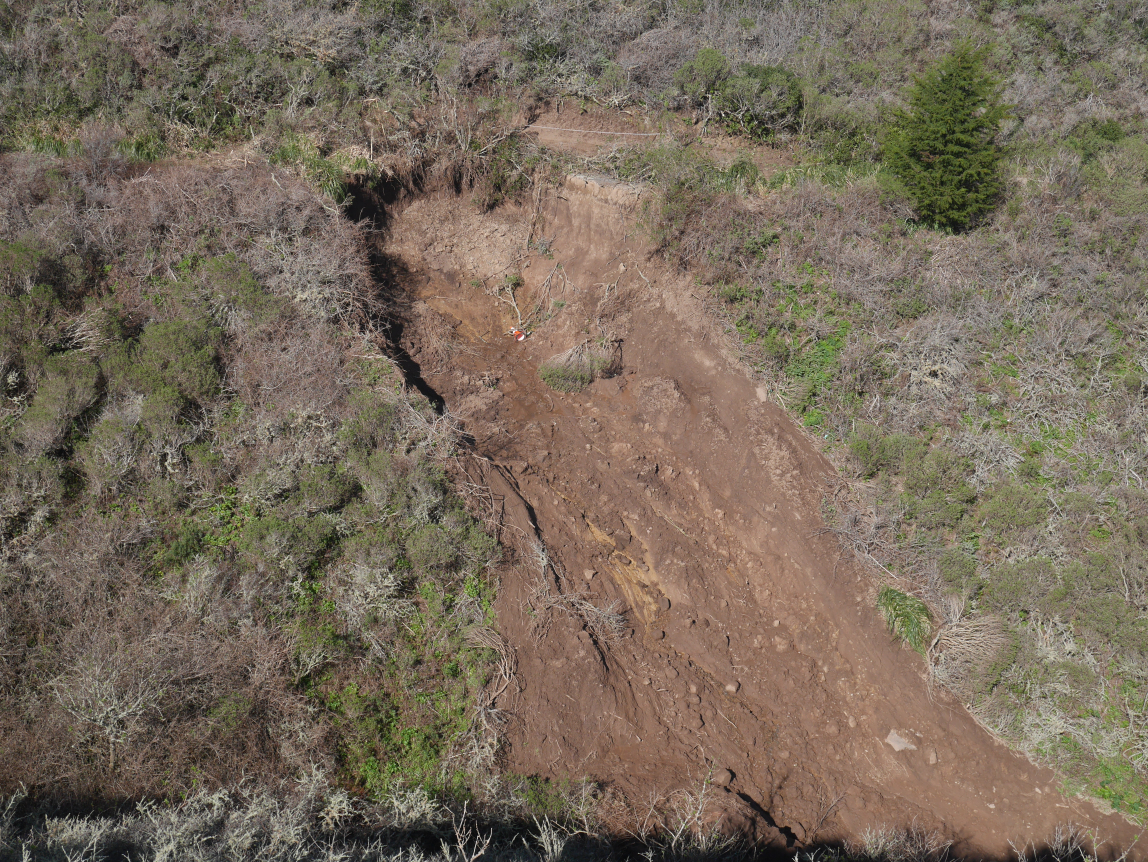
\includegraphics[width=0.75\linewidth]{img/P1020951_25} 

}

\caption{Landslide in San Pedro Creek watershed}\label{fig:modLandslide}
\end{figure}

Also see the relevant section in the San Pedro Creek Virtual Fieldtrip story map: Davis (\citeproc{ref-SanPedroCreekWatershedVirtualFieldtrip}{n.d.}).

Landslides detected in San Pedro Creek Watershed in Pacifica, CA, are in the SanPedro folder of extdata. Landslides were detected on aerial photography from 1941, 1955, 1975, 1983, and 1997 (Figure \ref{fig:modSPlandslides}), and confirmed in the field during a study in the early 2000s (Sims (\citeproc{ref-Sims2004}{2004}), Davis and Blesius (\citeproc{ref-DavisBlesius2015}{2015})) (Figure \ref{fig:modSedSourceStudy}).

\begin{Shaded}
\begin{Highlighting}[]
\FunctionTok{library}\NormalTok{(igisci); }\FunctionTok{library}\NormalTok{(sf); }\FunctionTok{library}\NormalTok{(tidyverse); }\FunctionTok{library}\NormalTok{(terra)}
\NormalTok{slides }\OtherTok{\textless{}{-}} \FunctionTok{st\_read}\NormalTok{(}\FunctionTok{ex}\NormalTok{(}\StringTok{"SanPedro/slideCentroids.shp"}\NormalTok{)) }\SpecialCharTok{\%\textgreater{}\%}
  \FunctionTok{mutate}\NormalTok{(}\AttributeTok{IsSlide =} \DecValTok{1}\NormalTok{)}
\NormalTok{slides}\SpecialCharTok{$}\NormalTok{Visible }\OtherTok{\textless{}{-}} \FunctionTok{factor}\NormalTok{(slides}\SpecialCharTok{$}\NormalTok{Visible)}
\NormalTok{trails }\OtherTok{\textless{}{-}} \FunctionTok{st\_read}\NormalTok{(}\FunctionTok{ex}\NormalTok{(}\StringTok{"SanPedro/trails.shp"}\NormalTok{))}
\NormalTok{streams }\OtherTok{\textless{}{-}} \FunctionTok{st\_read}\NormalTok{(}\FunctionTok{ex}\NormalTok{(}\StringTok{"SanPedro/streams.shp"}\NormalTok{))}
\NormalTok{wshed }\OtherTok{\textless{}{-}} \FunctionTok{st\_read}\NormalTok{(}\FunctionTok{ex}\NormalTok{(}\StringTok{"SanPedro/SPCWatershed.shp"}\NormalTok{))}
\end{Highlighting}
\end{Shaded}

\begin{Shaded}
\begin{Highlighting}[]
\FunctionTok{ggplot}\NormalTok{(}\AttributeTok{data=}\NormalTok{slides) }\SpecialCharTok{+} \FunctionTok{geom\_sf}\NormalTok{(}\FunctionTok{aes}\NormalTok{(}\AttributeTok{col=}\NormalTok{Visible)) }\SpecialCharTok{+} 
  \FunctionTok{scale\_color\_brewer}\NormalTok{(}\AttributeTok{palette=}\StringTok{"Spectral"}\NormalTok{) }\SpecialCharTok{+}
  \FunctionTok{geom\_sf}\NormalTok{(}\AttributeTok{data=}\NormalTok{streams, }\AttributeTok{col=}\StringTok{"blue"}\NormalTok{) }\SpecialCharTok{+}
  \FunctionTok{geom\_sf}\NormalTok{(}\AttributeTok{data=}\NormalTok{wshed, }\AttributeTok{fill=}\ConstantTok{NA}\NormalTok{)}
\end{Highlighting}
\end{Shaded}

\begin{figure}

{\centering \includegraphics[width=0.75\linewidth]{EnvDataScience_files/figure-latex/modSPlandslides-1} 

}

\caption{Landslides in San Pedro Creek watershed}\label{fig:modSPlandslides}
\end{figure}

\begin{figure}

{\centering \includegraphics[width=0.75\linewidth]{img/SedSource} 

}

\caption{Sediment source analysis}\label{fig:modSedSourceStudy}
\end{figure}

We'll create a logistic regression \index{logistic regression}to compare landslide probability to various environmental factors. We'll use elevation, slope, and other derivatives, distance to streams, distance to trails, and the results of a physical model predicting slope stability as a stability index (SI), using slope and soil transmissivity data.

At this point, we have data for \emph{occurrences} \index{occurrence data}of landslides, and so for each point we assign the dummy variable \texttt{IsSlide\ =\ 1}. We don't have any \emph{absence} \index{absence data}data, but we can create some using random points \index{random points}and assign them \texttt{IsSlide\ =\ 0}. It would probably be a good idea to avoid areas very close to the occurrences, but we'll just put random points everywhere and just remove the ones that don't have SI data.

For the random \ref{random} locations (Figure \ref{fig:modSPrandomPts}), we'll set a seed so for the book the results will stay the same; and if we're good with that since it doesn't really matter what seed we use, we might as well use the answer to everything: 42.

\begin{Shaded}
\begin{Highlighting}[]
\FunctionTok{library}\NormalTok{(terra)}
\NormalTok{elev }\OtherTok{\textless{}{-}} \FunctionTok{rast}\NormalTok{(}\FunctionTok{ex}\NormalTok{(}\StringTok{"SanPedro/dem.tif"}\NormalTok{))}
\NormalTok{SI }\OtherTok{\textless{}{-}} \FunctionTok{rast}\NormalTok{(}\FunctionTok{ex}\NormalTok{(}\StringTok{"SanPedro/SI.tif"}\NormalTok{))}
\NormalTok{npts }\OtherTok{\textless{}{-}} \FunctionTok{length}\NormalTok{(slides}\SpecialCharTok{$}\NormalTok{Visible) }\SpecialCharTok{*} \DecValTok{2} \CommentTok{\# up it a little to get enough after clip}
\FunctionTok{set.seed}\NormalTok{(}\DecValTok{42}\NormalTok{)}
\NormalTok{x }\OtherTok{\textless{}{-}} \FunctionTok{runif}\NormalTok{(npts, }\AttributeTok{min=}\FunctionTok{xmin}\NormalTok{(elev), }\AttributeTok{max=}\FunctionTok{xmax}\NormalTok{(elev))}
\NormalTok{y }\OtherTok{\textless{}{-}} \FunctionTok{runif}\NormalTok{(npts, }\AttributeTok{min=}\FunctionTok{ymin}\NormalTok{(elev), }\AttributeTok{max=}\FunctionTok{ymax}\NormalTok{(elev))}
\NormalTok{rsampsRaw }\OtherTok{\textless{}{-}} \FunctionTok{st\_as\_sf}\NormalTok{(}\FunctionTok{data.frame}\NormalTok{(x,y), }\AttributeTok{coords =} \FunctionTok{c}\NormalTok{(}\StringTok{"x"}\NormalTok{,}\StringTok{"y"}\NormalTok{), }\AttributeTok{crs=}\FunctionTok{crs}\NormalTok{(elev))}
\FunctionTok{ggplot}\NormalTok{(}\AttributeTok{data=}\NormalTok{rsampsRaw) }\SpecialCharTok{+} \FunctionTok{geom\_sf}\NormalTok{(}\AttributeTok{size=}\FloatTok{0.5}\NormalTok{) }\SpecialCharTok{+} 
  \FunctionTok{geom\_sf}\NormalTok{(}\AttributeTok{data=}\NormalTok{streams, }\AttributeTok{col=}\StringTok{"blue"}\NormalTok{) }\SpecialCharTok{+}
  \FunctionTok{geom\_sf}\NormalTok{(}\AttributeTok{data=}\NormalTok{wshed, }\AttributeTok{fill=}\ConstantTok{NA}\NormalTok{)}
\end{Highlighting}
\end{Shaded}

\begin{figure}

{\centering \includegraphics[width=0.75\linewidth]{EnvDataScience_files/figure-latex/modSPrandomPts-1} 

}

\caption{Raw random points}\label{fig:modSPrandomPts}
\end{figure}

Now we have twice as many random points as we have landslides, within the rectangular extend of the watershed, as defined by the elevation raster. We doubled these because we need to exclude some points, yet still have enough to be roughly as many random points as slides. We'll exclude:

\begin{itemize}
\tightlist
\item
  all points outside the watershed
\item
  points within 100 m of the landslide occurrences, the distance based on knowledge of the grain of landscape features (like spurs and swales) that might influence landslide occurrence
\end{itemize}

\begin{Shaded}
\begin{Highlighting}[]
\NormalTok{slideBuff }\OtherTok{\textless{}{-}} \FunctionTok{st\_buffer}\NormalTok{(slides, }\DecValTok{100}\NormalTok{)}
\NormalTok{wshedNoSlide }\OtherTok{\textless{}{-}} \FunctionTok{st\_difference}\NormalTok{(wshed, }\FunctionTok{st\_union}\NormalTok{(slideBuff))}
\end{Highlighting}
\end{Shaded}

First, we'll just see what \texttt{st\_difference()} returns:

\begin{Shaded}
\begin{Highlighting}[]
\FunctionTok{ggplot}\NormalTok{(wshedNoSlide) }\SpecialCharTok{+} \FunctionTok{geom\_sf}\NormalTok{(}\AttributeTok{fill=}\StringTok{"green"}\NormalTok{)}
\end{Highlighting}
\end{Shaded}

\begin{center}\includegraphics[width=0.75\linewidth]{EnvDataScience_files/figure-latex/unnamed-chunk-299-1} \end{center}

The 100 m buffer \index{buffer exclusion}excludes all areas around all landslides in the data set (Figure \ref{fig:modRandomBuffer}). We're going to run the model on specific years, but the best selection of landslide absences will be to exclude areas around all landslides we know of (Figure \ref{fig:modRandomeExcluded}).

\begin{Shaded}
\begin{Highlighting}[]
\FunctionTok{ggplot}\NormalTok{(}\AttributeTok{data=}\NormalTok{slides) }\SpecialCharTok{+} \FunctionTok{geom\_sf}\NormalTok{(}\FunctionTok{aes}\NormalTok{(}\AttributeTok{col=}\NormalTok{Visible)) }\SpecialCharTok{+} 
  \FunctionTok{scale\_color\_brewer}\NormalTok{(}\AttributeTok{palette=}\StringTok{"Spectral"}\NormalTok{) }\SpecialCharTok{+}
  \FunctionTok{geom\_sf}\NormalTok{(}\AttributeTok{data=}\NormalTok{streams, }\AttributeTok{col=}\StringTok{"blue"}\NormalTok{) }\SpecialCharTok{+}
  \FunctionTok{geom\_sf}\NormalTok{(}\AttributeTok{data=}\NormalTok{wshedNoSlide, }\AttributeTok{fill=}\ConstantTok{NA}\NormalTok{)}
\end{Highlighting}
\end{Shaded}

\begin{figure}

{\centering \includegraphics[width=0.75\linewidth]{EnvDataScience_files/figure-latex/modRandomBuffer-1} 

}

\caption{Landslides and buffers to exclude from random points}\label{fig:modRandomBuffer}
\end{figure}

\begin{Shaded}
\begin{Highlighting}[]
\NormalTok{rsamps }\OtherTok{\textless{}{-}} \FunctionTok{st\_intersection}\NormalTok{(rsampsRaw,wshedNoSlide) }\SpecialCharTok{\%\textgreater{}\%}
  \FunctionTok{mutate}\NormalTok{(}\AttributeTok{IsSlide =} \DecValTok{0}\NormalTok{)}
\NormalTok{allPts }\OtherTok{\textless{}{-}} \FunctionTok{bind\_rows}\NormalTok{(slides, rsamps)}
\end{Highlighting}
\end{Shaded}

\begin{Shaded}
\begin{Highlighting}[]
\FunctionTok{ggplot}\NormalTok{(}\AttributeTok{data=}\NormalTok{allPts) }\SpecialCharTok{+} \FunctionTok{geom\_sf}\NormalTok{(}\FunctionTok{aes}\NormalTok{(}\AttributeTok{col=}\NormalTok{IsSlide)) }\SpecialCharTok{+} 
  \FunctionTok{geom\_sf}\NormalTok{(}\AttributeTok{data=}\NormalTok{streams, }\AttributeTok{col=}\StringTok{"blue"}\NormalTok{) }\SpecialCharTok{+}
  \FunctionTok{geom\_sf}\NormalTok{(}\AttributeTok{data=}\NormalTok{wshed, }\AttributeTok{fill=}\ConstantTok{NA}\NormalTok{)}
\end{Highlighting}
\end{Shaded}

\begin{figure}

{\centering \includegraphics[width=0.75\linewidth]{EnvDataScience_files/figure-latex/modRandomeExcluded-1} 

}

\caption{Landslides and random points (excluded from slide buffers)}\label{fig:modRandomeExcluded}
\end{figure}

Now we'll derive some environmental variables \index{environmental raster variables}as rasters and extract their values\index{extraction from rasters} to the slide/noslide point data set. We'll use the \texttt{shade} function to create a \texttt{hillshade} raster with the sun at the average noon angle from the south.

\begin{Shaded}
\begin{Highlighting}[]
\NormalTok{slidesV }\OtherTok{\textless{}{-}} \FunctionTok{vect}\NormalTok{(allPts)}
\NormalTok{strms }\OtherTok{\textless{}{-}} \FunctionTok{rasterize}\NormalTok{(}\FunctionTok{vect}\NormalTok{(streams),elev)}
\NormalTok{tr }\OtherTok{\textless{}{-}} \FunctionTok{rasterize}\NormalTok{(}\FunctionTok{vect}\NormalTok{(trails),elev)}
\NormalTok{stD }\OtherTok{\textless{}{-}}\NormalTok{ terra}\SpecialCharTok{::}\FunctionTok{distance}\NormalTok{(strms); }\FunctionTok{names}\NormalTok{(stD) }\OtherTok{=} \StringTok{"stD"}
\NormalTok{trD }\OtherTok{\textless{}{-}}\NormalTok{ terra}\SpecialCharTok{::}\FunctionTok{distance}\NormalTok{(tr); }\FunctionTok{names}\NormalTok{(trD) }\OtherTok{=} \StringTok{"trD"}
\NormalTok{slope }\OtherTok{\textless{}{-}} \FunctionTok{terrain}\NormalTok{(elev, }\AttributeTok{v=}\StringTok{"slope"}\NormalTok{)}
\NormalTok{curv }\OtherTok{\textless{}{-}} \FunctionTok{terrain}\NormalTok{(slope, }\AttributeTok{v=}\StringTok{"slope"}\NormalTok{)}
\NormalTok{aspect }\OtherTok{\textless{}{-}} \FunctionTok{terrain}\NormalTok{(elev, }\AttributeTok{v=}\StringTok{"aspect"}\NormalTok{)}
\NormalTok{hillshade }\OtherTok{\textless{}{-}} \FunctionTok{shade}\NormalTok{(slope}\SpecialCharTok{/}\DecValTok{180}\SpecialCharTok{*}\NormalTok{pi,aspect}\SpecialCharTok{/}\DecValTok{180}\SpecialCharTok{*}\NormalTok{pi,}\AttributeTok{angle=}\DecValTok{53}\NormalTok{,}\AttributeTok{direction=}\DecValTok{180}\NormalTok{)}
\NormalTok{elev\_ex }\OtherTok{\textless{}{-}}\NormalTok{ terra}\SpecialCharTok{::}\FunctionTok{extract}\NormalTok{(elev, slidesV) }\SpecialCharTok{\%\textgreater{}\%} 
  \FunctionTok{rename}\NormalTok{(}\AttributeTok{elev=}\NormalTok{dem) }\SpecialCharTok{\%\textgreater{}\%}\NormalTok{ dplyr}\SpecialCharTok{::}\FunctionTok{select}\NormalTok{(}\SpecialCharTok{{-}}\NormalTok{ID)}
\NormalTok{SI\_ex }\OtherTok{\textless{}{-}}\NormalTok{ terra}\SpecialCharTok{::}\FunctionTok{extract}\NormalTok{(SI, slidesV) }\SpecialCharTok{\%\textgreater{}\%}\NormalTok{ dplyr}\SpecialCharTok{::}\FunctionTok{select}\NormalTok{(}\SpecialCharTok{{-}}\NormalTok{ID)}
\NormalTok{slope\_ex }\OtherTok{\textless{}{-}}\NormalTok{ terra}\SpecialCharTok{::}\FunctionTok{extract}\NormalTok{(slope, slidesV) }\SpecialCharTok{\%\textgreater{}\%}\NormalTok{ dplyr}\SpecialCharTok{::}\FunctionTok{select}\NormalTok{(}\SpecialCharTok{{-}}\NormalTok{ID)}
\NormalTok{curv\_ex }\OtherTok{\textless{}{-}}\NormalTok{ terra}\SpecialCharTok{::}\FunctionTok{extract}\NormalTok{(curv, slidesV) }\SpecialCharTok{\%\textgreater{}\%} 
  \FunctionTok{rename}\NormalTok{(}\AttributeTok{curv =}\NormalTok{ slope) }\SpecialCharTok{\%\textgreater{}\%}\NormalTok{ dplyr}\SpecialCharTok{::}\FunctionTok{select}\NormalTok{(}\SpecialCharTok{{-}}\NormalTok{ID)}
\NormalTok{hillshade\_ex }\OtherTok{\textless{}{-}}\NormalTok{ terra}\SpecialCharTok{::}\FunctionTok{extract}\NormalTok{(hillshade, slidesV) }\SpecialCharTok{\%\textgreater{}\%} 
\NormalTok{  dplyr}\SpecialCharTok{::}\FunctionTok{select}\NormalTok{(}\SpecialCharTok{{-}}\NormalTok{ID)}
\NormalTok{stD\_ex }\OtherTok{\textless{}{-}}\NormalTok{ terra}\SpecialCharTok{::}\FunctionTok{extract}\NormalTok{(stD, slidesV) }\SpecialCharTok{\%\textgreater{}\%}\NormalTok{ dplyr}\SpecialCharTok{::}\FunctionTok{select}\NormalTok{(}\SpecialCharTok{{-}}\NormalTok{ID)}
\NormalTok{trD\_ex }\OtherTok{\textless{}{-}}\NormalTok{ terra}\SpecialCharTok{::}\FunctionTok{extract}\NormalTok{(trD, slidesV) }\SpecialCharTok{\%\textgreater{}\%}\NormalTok{ dplyr}\SpecialCharTok{::}\FunctionTok{select}\NormalTok{(}\SpecialCharTok{{-}}\NormalTok{ID)}
\NormalTok{slidePts }\OtherTok{\textless{}{-}} \FunctionTok{cbind}\NormalTok{(allPts,elev\_ex,SI\_ex,slope\_ex,curv\_ex,hillshade\_ex,stD\_ex,trD\_ex)}
\NormalTok{slidesData }\OtherTok{\textless{}{-}} \FunctionTok{as.data.frame}\NormalTok{(slidePts) }\SpecialCharTok{\%\textgreater{}\%}
                            \FunctionTok{filter}\NormalTok{(}\SpecialCharTok{!}\FunctionTok{is.nan}\NormalTok{(SI)) }\SpecialCharTok{\%\textgreater{}\%} \FunctionTok{st\_as\_sf}\NormalTok{(}\AttributeTok{crs=}\FunctionTok{st\_crs}\NormalTok{(slides))}
\end{Highlighting}
\end{Shaded}

We'll filter \index{filter for year}for just the slides in the 1983 imagery, and for the model also include all of the random points (detected with \texttt{NA} values for Visible):

\begin{Shaded}
\begin{Highlighting}[]
\NormalTok{slides83 }\OtherTok{\textless{}{-}}\NormalTok{ slidesData }\SpecialCharTok{\%\textgreater{}\%} \FunctionTok{filter}\NormalTok{(Visible }\SpecialCharTok{==} \DecValTok{1983}\NormalTok{)}
\NormalTok{slides83plusr }\OtherTok{\textless{}{-}}\NormalTok{ slidesData }\SpecialCharTok{\%\textgreater{}\%} \FunctionTok{filter}\NormalTok{(Visible }\SpecialCharTok{==} \DecValTok{1983} \SpecialCharTok{|} \FunctionTok{is.na}\NormalTok{(Visible))}
\end{Highlighting}
\end{Shaded}

The logistic regression in the glm model uses the \emph{binomial} family\index{binomial family glm}:

\begin{Shaded}
\begin{Highlighting}[]
\FunctionTok{summary}\NormalTok{(}\FunctionTok{glm}\NormalTok{(IsSlide }\SpecialCharTok{\textasciitilde{}}\NormalTok{ SI }\SpecialCharTok{+}\NormalTok{ curv }\SpecialCharTok{+}\NormalTok{ elev }\SpecialCharTok{+}\NormalTok{ slope }\SpecialCharTok{+}\NormalTok{ hillshade }\SpecialCharTok{+}\NormalTok{ stD }\SpecialCharTok{+}\NormalTok{ trD, }
            \AttributeTok{family=}\NormalTok{binomial, }\AttributeTok{data=}\NormalTok{slides83plusr))}
\end{Highlighting}
\end{Shaded}

\begin{verbatim}
## 
## Call:
## glm(formula = IsSlide ~ SI + curv + elev + slope + hillshade + 
##     stD + trD, family = binomial, data = slides83plusr)
## 
## Coefficients:
##               Estimate Std. Error z value Pr(>|z|)    
## (Intercept)  0.1428138  1.0618829   0.134  0.89301    
## SI          -1.8191092  0.3639254  -4.999 5.78e-07 ***
## curv         0.0059240  0.0113658   0.521  0.60222    
## elev        -0.0025053  0.0014399  -1.740  0.08187 .  
## slope        0.0623188  0.0211011   2.953  0.00314 ** 
## hillshade    2.6972342  0.6603871   4.084 4.42e-05 ***
## stD         -0.0052633  0.0019765  -2.663  0.00775 ** 
## trD         -0.0020734  0.0006532  -3.174  0.00150 ** 
## ---
## Signif. codes:  0 '***' 0.001 '**' 0.01 '*' 0.05 '.' 0.1 ' ' 1
## 
## (Dispersion parameter for binomial family taken to be 1)
## 
##     Null deviance: 668.29  on 483  degrees of freedom
## Residual deviance: 402.90  on 476  degrees of freedom
##   (85 observations deleted due to missingness)
## AIC: 418.9
## 
## Number of Fisher Scoring iterations: 8
\end{verbatim}

So while we might want to make sure that we've picked the right variables, some conclusions from this might be that stability index (\texttt{SI}) is not surprisingly a strong predictor of landslides, but also that other than elevation and curvature, the other variables are also significant.

\subsubsection{Map the logistic result}\label{map-the-logistic-result}

\index{logistic result map}We should be able to map the results; we just need to use the formula for the model, which in our case will have six explanatory variables SI (\(X_1\)), elev (\(X_2\)), slope (\(X_3\)), hillshade (\(X_4\)), stD (\(X_5\)), and trD (\(X_6\)): \[p = \frac{e^{b_0+b_1X_1+b_2X_2+b_3X_3+b_4X_4+b_5X_5}}{1+e^{b_0+b_1X_1+b_2X_2+b_3X_3+b_4X_4+b_5X_5}}\]

Then we retrieve the coefficients with \texttt{coef()} and use map algebra to create the prediction map, including dots for the landslides actually observed in 1983 (Figure \ref{fig:modLogisticPredict}).

\begin{Shaded}
\begin{Highlighting}[]
\FunctionTok{library}\NormalTok{(tmap)}
\NormalTok{SI\_stD\_model }\OtherTok{\textless{}{-}} \FunctionTok{glm}\NormalTok{(IsSlide }\SpecialCharTok{\textasciitilde{}}\NormalTok{ SI }\SpecialCharTok{+}\NormalTok{ slope }\SpecialCharTok{+}\NormalTok{ hillshade }\SpecialCharTok{+}\NormalTok{ stD }\SpecialCharTok{+}\NormalTok{ trD, }\AttributeTok{family=}\NormalTok{binomial, }
                    \AttributeTok{data=}\NormalTok{slides83plusr)}
\NormalTok{b0 }\OtherTok{\textless{}{-}} \FunctionTok{coef}\NormalTok{(SI\_stD\_model)[}\DecValTok{1}\NormalTok{]}
\NormalTok{b1 }\OtherTok{\textless{}{-}} \FunctionTok{coef}\NormalTok{(SI\_stD\_model)[}\DecValTok{2}\NormalTok{]}
\NormalTok{b2 }\OtherTok{\textless{}{-}} \FunctionTok{coef}\NormalTok{(SI\_stD\_model)[}\DecValTok{3}\NormalTok{]}
\NormalTok{b3 }\OtherTok{\textless{}{-}} \FunctionTok{coef}\NormalTok{(SI\_stD\_model)[}\DecValTok{4}\NormalTok{]}
\NormalTok{b4 }\OtherTok{\textless{}{-}} \FunctionTok{coef}\NormalTok{(SI\_stD\_model)[}\DecValTok{5}\NormalTok{]}
\NormalTok{b5 }\OtherTok{\textless{}{-}} \FunctionTok{coef}\NormalTok{(SI\_stD\_model)[}\DecValTok{6}\NormalTok{]}
\NormalTok{predictionMap }\OtherTok{\textless{}{-}}\NormalTok{ (}\FunctionTok{exp}\NormalTok{(b0}\SpecialCharTok{+}\NormalTok{b1}\SpecialCharTok{*}\NormalTok{SI}\SpecialCharTok{+}\NormalTok{b2}\SpecialCharTok{*}\NormalTok{slope}\SpecialCharTok{+}\NormalTok{b3}\SpecialCharTok{*}\NormalTok{hillshade}\SpecialCharTok{+}\NormalTok{b4}\SpecialCharTok{*}\NormalTok{stD}\SpecialCharTok{+}\NormalTok{b5}\SpecialCharTok{*}\NormalTok{trD))}\SpecialCharTok{/}
\NormalTok{  (}\DecValTok{1} \SpecialCharTok{+} \FunctionTok{exp}\NormalTok{(b0}\SpecialCharTok{+}\NormalTok{b1}\SpecialCharTok{*}\NormalTok{SI}\SpecialCharTok{+}\NormalTok{b2}\SpecialCharTok{*}\NormalTok{slope}\SpecialCharTok{+}\NormalTok{b3}\SpecialCharTok{*}\NormalTok{hillshade}\SpecialCharTok{+}\NormalTok{b4}\SpecialCharTok{*}\NormalTok{stD}\SpecialCharTok{+}\NormalTok{b5}\SpecialCharTok{*}\NormalTok{trD))}
\FunctionTok{names}\NormalTok{(predictionMap) }\OtherTok{\textless{}{-}} \StringTok{"probability}\SpecialCharTok{\textbackslash{}n}\StringTok{1983"}
\FunctionTok{tm\_shape}\NormalTok{(predictionMap) }\SpecialCharTok{+}
    \FunctionTok{tm\_raster}\NormalTok{(}\AttributeTok{col.scale=}\FunctionTok{tm\_scale\_continuous}\NormalTok{(}\AttributeTok{values=}\StringTok{"carto.peach"}\NormalTok{)) }\SpecialCharTok{+}
  \FunctionTok{tm\_shape}\NormalTok{(streams) }\SpecialCharTok{+} \FunctionTok{tm\_lines}\NormalTok{(}\AttributeTok{col=}\StringTok{"blue"}\NormalTok{) }\SpecialCharTok{+}
  \FunctionTok{tm\_shape}\NormalTok{(wshed) }\SpecialCharTok{+} \FunctionTok{tm\_borders}\NormalTok{(}\AttributeTok{col=}\StringTok{"black"}\NormalTok{) }\SpecialCharTok{+}
  \FunctionTok{tm\_shape}\NormalTok{(slides83) }\SpecialCharTok{+} 
    \FunctionTok{tm\_dots}\NormalTok{(}\AttributeTok{fill=}\StringTok{"purple"}\NormalTok{, }\AttributeTok{size=}\FloatTok{0.25}\NormalTok{,}
            \AttributeTok{size.legend=}\FunctionTok{tm\_legend}\NormalTok{(}\StringTok{"1983 slides"}\NormalTok{,}\AttributeTok{frame=}\NormalTok{F)) }\SpecialCharTok{+}
  \FunctionTok{tm\_title}\NormalTok{(}\StringTok{"Landslides predicted by}\SpecialCharTok{\textbackslash{}n}\StringTok{SI, slope, hillshade, streamD, trailD"}\NormalTok{) }\SpecialCharTok{+} 
  \FunctionTok{tm\_graticules}\NormalTok{(}\AttributeTok{lines=}\NormalTok{F)}
\end{Highlighting}
\end{Shaded}

\begin{figure}

{\centering \includegraphics[width=0.75\linewidth]{EnvDataScience_files/figure-latex/modLogisticPredict-1} 

}

\caption{Logistic model prediction of 1983 landslide probability}\label{fig:modLogisticPredict}
\end{figure}

\subsection{Poisson regression}\label{poisson-regression}

Poission regression (\texttt{family\ =\ poisson} in glm) is for analyzing counts\index{poisson model}. You might use this to determine which variables are significant predictors, or you might want to see where or when counts are particularly high, or higher than expected. Or it might be applied to compare groupings. For example, if instead of looking at differences among rock types in Sinking Cove based on chemical properties in water samples or measurements (where we applied ANOVA), we looked at differences in fish counts, that might be an application of poisson regression, as long as other data assumptions hold.

\subsubsection{Seabird Poisson Model}\label{seabird-poisson-model}

This \index{seabird poisson model}model is further developed in a separate case study where we'll map a prediction, but we'll look at the basics for applying a poisson family model in glm: \emph{seabird observations}. The data is potentially suitable since its counts with known time intervals of observation effort and initial review of the data suggests that the mean of counts is reasonably similar to the variance. The data was collected through the ACCESS program (\emph{Applied California Current Ecosystem Studies} (\citeproc{ref-ACCESS}{n.d.})) and a thorough analysis is provided by Studwell et al. (\citeproc{ref-Studwell2017}{2017}).

\begin{Shaded}
\begin{Highlighting}[]
\FunctionTok{library}\NormalTok{(igisci); }\FunctionTok{library}\NormalTok{(sf); }\FunctionTok{library}\NormalTok{(tidyverse); }\FunctionTok{library}\NormalTok{(tmap)}
\FunctionTok{library}\NormalTok{(maptiles)}
\NormalTok{transects }\OtherTok{\textless{}{-}} \FunctionTok{st\_read}\NormalTok{(}\FunctionTok{ex}\NormalTok{(}\StringTok{"SFmarine/transects.shp"}\NormalTok{))}
\end{Highlighting}
\end{Shaded}

One of the seabirds studies, the black-footed albatross\index{black-footed albatross}, has the lowest counts (so a relatively rare bird\index{bird}), and studies of its distribution may be informative. We'll look at counts collected during transect cruises\index{bird transects} in July 2006 (Figure \ref{fig:modAlbatrossCounts}).

\begin{Shaded}
\begin{Highlighting}[]
\FunctionTok{tmap\_mode}\NormalTok{(}\StringTok{"plot"}\NormalTok{)}
\NormalTok{transJul2006 }\OtherTok{\textless{}{-}}\NormalTok{ transects }\SpecialCharTok{\%\textgreater{}\%}
  \FunctionTok{filter}\NormalTok{(month}\SpecialCharTok{==}\DecValTok{7} \SpecialCharTok{\&}\NormalTok{ year}\SpecialCharTok{==}\DecValTok{2006} \SpecialCharTok{\&}\NormalTok{ avg\_tem}\SpecialCharTok{\textgreater{}}\DecValTok{0} \SpecialCharTok{\&}\NormalTok{ avg\_sal}\SpecialCharTok{\textgreater{}}\DecValTok{0} \SpecialCharTok{\&}\NormalTok{ avg\_fluo}\SpecialCharTok{\textgreater{}}\DecValTok{0}\NormalTok{)}
\FunctionTok{tm\_basemap}\NormalTok{(}\StringTok{"Esri.NatGeoWorldMap"}\NormalTok{) }\SpecialCharTok{+}
  \FunctionTok{tm\_shape}\NormalTok{(transJul2006) }\SpecialCharTok{+} \FunctionTok{tm\_symbols}\NormalTok{(}\AttributeTok{fill=}\StringTok{"bfal"}\NormalTok{, }\AttributeTok{size=}\StringTok{"bfal"}\NormalTok{,}
                                      \AttributeTok{fill.scale=}\FunctionTok{tm\_scale\_continuous}\NormalTok{(}\AttributeTok{values=}\StringTok{"Greens"}\NormalTok{))}
\end{Highlighting}
\end{Shaded}

\begin{figure}

{\centering \includegraphics[width=0.75\linewidth]{EnvDataScience_files/figure-latex/modAlbatrossCounts-1} 

}

\caption{Black-footed albatross counts, July 2006}\label{fig:modAlbatrossCounts}
\end{figure}

Prior studies have suggested that temperature\index{temperature}, salinity\index{salinity}, fluorescence\index{fluorescence}, depth\index{depth}, and various distances\index{distance (as explanatory variable)} might be good explanatory variables to use to look at spatial patterns, so we'll use these in the model.

\begin{Shaded}
\begin{Highlighting}[]
\FunctionTok{summary}\NormalTok{(}\FunctionTok{glm}\NormalTok{(bfal}\SpecialCharTok{\textasciitilde{}}\NormalTok{avg\_tem }\SpecialCharTok{+}\NormalTok{ avg\_sal }\SpecialCharTok{+}\NormalTok{ avg\_fluo }\SpecialCharTok{+}\NormalTok{ avg\_dep }\SpecialCharTok{+}
\NormalTok{            dist\_land }\SpecialCharTok{+}\NormalTok{ dist\_isla }\SpecialCharTok{+}\NormalTok{ dist\_200m }\SpecialCharTok{+}\NormalTok{ dist\_cord, }
            \AttributeTok{data=}\NormalTok{transJul2006, }\AttributeTok{family=}\NormalTok{poisson))}
\end{Highlighting}
\end{Shaded}

\begin{verbatim}
## 
## Call:
## glm(formula = bfal ~ avg_tem + avg_sal + avg_fluo + avg_dep + 
##     dist_land + dist_isla + dist_200m + dist_cord, family = poisson, 
##     data = transJul2006)
## 
## Coefficients:
##               Estimate Std. Error z value Pr(>|z|)    
## (Intercept) -1.754e+02  7.032e+01  -2.495  0.01260 *  
## avg_tem      7.341e-01  3.479e-01   2.110  0.03482 *  
## avg_sal      5.202e+00  2.097e+00   2.480  0.01312 *  
## avg_fluo    -6.978e-01  1.217e+00  -0.574  0.56626    
## avg_dep     -3.561e-03  8.229e-04  -4.328 1.51e-05 ***
## dist_land   -2.197e-04  6.194e-05  -3.547  0.00039 ***
## dist_isla    1.372e-05  1.778e-05   0.771  0.44043    
## dist_200m   -4.696e-04  1.037e-04  -4.528 5.95e-06 ***
## dist_cord   -5.213e-06  1.830e-05  -0.285  0.77570    
## ---
## Signif. codes:  0 '***' 0.001 '**' 0.01 '*' 0.05 '.' 0.1 ' ' 1
## 
## (Dispersion parameter for poisson family taken to be 1)
## 
##     Null deviance: 152.14  on 206  degrees of freedom
## Residual deviance: 105.73  on 198  degrees of freedom
## AIC: 160.37
## 
## Number of Fisher Scoring iterations: 7
\end{verbatim}

We can see in the model coefficients\index{model coefficients} table several predictive variables that appear to be significant, which we'll want to explore further, and also map the results as we did with Sierra temperature data.

\begin{itemize}
\tightlist
\item
  avg\_tem
\item
  avg\_sal
\item
  avg\_dep
\item
  dist\_land
\item
  dist\_200m
\end{itemize}

\textbf{Note} R will allow you to run glm on any family, but it's up to you to make sure it's appropriate. For example, if you provide a response variable that is \emph{not} count data or doesn't fit the requirements for a poisson model, R will create a result but it's bogus.

\section{Other modeling methods}\label{other-modeling-methods}

\subsection{Curve fitting}\label{curve-fitting}

In general, what we're doing with linear models and other approaches can be considered curve fitting, and we've seen how we can manipulate our data by modeling with transformed data, at least log-transformed, then applied to a linear model using \texttt{lm}. We've also looked a bit at generalized linear models with \texttt{glm}, but there are other methods such as:

\begin{itemize}
\tightlist
\item
  \texttt{poly} -- for polynomials
\item
  \texttt{nls} -- for nonlinear models
\end{itemize}

In the addenda to this book, the Curve Fitting chapter explores a bit of polynomial models and nonlinear models, and you might want to have a look:

\url{https://bookdown.org/igisc/EnvDataSciAddenda/curve-fitting.html}

\subsection{Models employing machine learning}\label{models-employing-machine-learning}

Models using machine learning \index{machine learning}algorithms are commonly used in data science, fitting with its general exploratory and data-mining approach. There are many machine learning algorithms, and many resources for learning more about them, but they all share a basically black-box approach where a collection of variables are explored for patterns in input variables that help to explain a response variable. The latter is similar to more conventional statistical modeling describe above, with the difference being the machine learning approach -- think of robots going through your data looking for connections.

We'll explore machine learning methods in the next chapter when we attempt to use them to classify satellite imagery, an important environmental application.

\pagebreak

\section{Exercises: Modeling}\label{exercises-modeling}

\begin{exercise}
Add \texttt{LATITUDE} as a second independent variable after \texttt{ELEVATION} in the model predicting February temperatures. (You may need to see 7.1 for how to retain \texttt{LATITUDE} and \texttt{LONGITUDE} as variables, using \texttt{remove=F}) Then you'll need to change the regression formula to include both \texttt{ELEVATION\ +\ LATITUDE}. First derive and display the model summary results, and then answer the questions -- is the explanation better based on the \(r^2\)?
\end{exercise}

\begin{exercise}
Now map the \textbf{predictions} and \textbf{residuals}.
\end{exercise}

\begin{center}\includegraphics[width=0.75\linewidth]{img/model_ex2a} \end{center}

\begin{center}\includegraphics[width=0.75\linewidth]{img/model_ex2b} \end{center}

\begin{exercise}
Can you see any potential for additional variables? What evidence might there be for local effects like topographically related microclimatology?
\end{exercise}

\begin{exercise}
Next we'll build and display a prediction raster from the above model, but we'll start by deriving the coefficients -- \texttt{b0}, \texttt{b1}, and \texttt{b2} -- that we'll need for the map algebra in the next step.
\end{exercise}

\begin{exercise}

To create the prediction raster we'll need a latitude raster. Use the following code to create a raster of the same dimensions as \texttt{elevSierra}, but with latitude assigned as z values to the cells. Then build and display a raster \textbf{prediction of temperature} from the model and the two explanatory rasters.

\begin{verbatim}
lats <- yFromCell(elevSierra, 1:ncell(elevSierra))
latitude <- setValues(elevSierra,lats)
\end{verbatim}

\end{exercise}

\begin{center}\includegraphics[width=0.75\linewidth]{img/model_ex5} \end{center}

\begin{exercise}
Modify the code for the San Pedro Creek Watershed logistical model (10.5.2) to analyze 1975 landslides. Are the conclusions different?
\end{exercise}

\begin{center}\includegraphics[width=0.75\linewidth]{img/model_ex6} \end{center}

\begin{exercise}
Optionally, using your own data that should have location information as well as other attributes, create a statistical model of your choice, and provide your assessment of the results, a prediction map, and where appropriate mapped residuals. You'll probably want to create a new project for this with a \texttt{data} folder.
\end{exercise}

\begin{exercise}
Optionally, using your own data but with no location data needed, create a glm binomial model. If you don't have anything obvious, consider doing something like the study of a pet dog panting based on temperature. \url{https://bscheng.com/2016/10/23/logistic-regression-in-r/}
\end{exercise}

\chapter{Imagery and Classification Models}\label{imagery}

\begin{center}\includegraphics[width=0.75\linewidth]{EnvDataScience_files/figure-latex/unnamed-chunk-309-1} \end{center}

This chapter explores the use of satellite imagery\index{imagery, satellite}, such as this Sentinel-2\index{Sentinel-2} scene (from 28 June 2021) of part of the northern Sierra Nevada, CA, to Pyramid Lake, NV, including display methods (such as the ``false color''\index{false-color} above) and imagery analysis methods. After we've learned how to read the data and cropped it to fit our study area in Red Clover Valley, we'll try some machine language classifiers to see if we can make sense of the patterns of hydric to xeric vegetation in a meadow under active restoration.

Image analysis methods are important for environmental research and are covered much more thoroughly in the discipline of \emph{remote sensing}\index{remote sensing}. Some key things to learn more about are the nature of the electromagnetic spectrum and especially bands of that spectrum\index{electromagnetic spectrum} that are informative for land cover\index{land cover} and especially vegetation\index{vegetation} detection, and the process of imagery classification\index{classification, imagery}. We'll be using satellite imagery\index{satellite imagery} that includes a range of the electromagnetic spectrum from visible to short-wave infrared\index{infrared}.

\section{Reading and Displaying Sentinel-2 Imagery}\label{reading-and-displaying-sentinel-2-imagery}

We'll work with 10 and 20 m Sentinel-2 data downloaded from \emph{Copernicus Open Access Hub} (\citeproc{ref-Copernicus}{n.d.}) \index{Copernicus (ESA site for Sentinel imagery)}as an entire scene from 20210602 and 20210628, providing cloud-free imagery of Red Clover Valley \index{Red Clover Valley}in the northern Sierra Nevada\index{Sierra Nevada}, where we are doing research on biogeochemical cycles \index{biogeochemical cycles} and carbon sequestration \index{carbon sequestration}from meadow restoration\index{restoration} with The Sierra Fund (\emph{Clover Valley Ranch Restoration, the Sierra Fund} (\citeproc{ref-TSF_CV}{n.d.})).

Download the image zip files from\ldots{}

\url{https://sfsu.box.com/s/zx9rvbxdss03rammy7d72rb3uumfzjbf}

\ldots and extract into the folder \texttt{\textasciitilde{}/sentinel2/} -- the \texttt{\textasciitilde{}} referring to your Home folder (typically \texttt{Documents}). (See the code below to see how one of the two images is read.) Make sure the folders stored there have names ending in \texttt{.SAFE}. The following are the two we'll be using:

\begin{itemize}
\tightlist
\item
  \texttt{S2B\_MSIL2A\_20210603T184919\_N0300\_R113\_T10TGK\_20210603T213609.SAFE}
\item
  \texttt{S2A\_MSIL2A\_20210628T184921\_N0300\_R113\_T10TGK\_20210628T230915.SAFE}
\end{itemize}

\begin{Shaded}
\begin{Highlighting}[]
\FunctionTok{library}\NormalTok{(stringr)}
\FunctionTok{library}\NormalTok{(terra)}
\NormalTok{imgFolder }\OtherTok{\textless{}{-}} \FunctionTok{paste0}\NormalTok{(}\StringTok{"S2A\_MSIL2A\_20210628T184921\_N0300\_R113\_T10TGK\_20210628T230915."}\NormalTok{,}
                    \StringTok{"SAFE}\SpecialCharTok{\textbackslash{}\textbackslash{}}\StringTok{GRANULE}\SpecialCharTok{\textbackslash{}\textbackslash{}}\StringTok{L2A\_T10TGK\_A031427\_20210628T185628"}\NormalTok{)}
\NormalTok{img20mFolder }\OtherTok{\textless{}{-}} \FunctionTok{paste0}\NormalTok{(}\StringTok{"\textasciitilde{}/sentinel2/"}\NormalTok{,imgFolder,}\StringTok{"}\SpecialCharTok{\textbackslash{}\textbackslash{}}\StringTok{IMG\_DATA}\SpecialCharTok{\textbackslash{}\textbackslash{}}\StringTok{R20m"}\NormalTok{)}
\NormalTok{imgDateTime }\OtherTok{\textless{}{-}} \FunctionTok{str\_sub}\NormalTok{(imgFolder,}\DecValTok{12}\NormalTok{,}\DecValTok{26}\NormalTok{)}
\NormalTok{imgDateTime}
\end{Highlighting}
\end{Shaded}

\begin{verbatim}
## [1] "20210628T184921"
\end{verbatim}

\begin{Shaded}
\begin{Highlighting}[]
\NormalTok{imgDate }\OtherTok{\textless{}{-}} \FunctionTok{str\_sub}\NormalTok{(imgDateTime,}\DecValTok{1}\NormalTok{,}\DecValTok{8}\NormalTok{)}
\end{Highlighting}
\end{Shaded}

As documented at \emph{Copernicus Open Access Hub} (\citeproc{ref-Copernicus}{n.d.}), Sentinel-2 imagery is collected at three resolutions\index{resolution, imagery}, with the most bands at the coarsest (60 m) resolution. The bands added at that coarsest resolution are not critical for our work as they relate to oceanographic and atmospheric research, and our focus will be on land cover\index{land cover} and vegetation\index{vegetation} in a terrestrial area. So we'll work with four bands\index{bands, imagery} at 10 m and an additional six bands at 20 m resolution:

10 m bands

\begin{itemize}
\tightlist
\item
  B02 - Blue 0.490 \(\mu\)m
\item
  B03 - Green 0.560 \(\mu\)m
\item
  B04 - Red 0.665 \(\mu\)m
\item
  B08 - NIR 0.842 \(\mu\)m
\end{itemize}

20 m bands

\begin{itemize}
\tightlist
\item
  B02 - Blue 0.490 \(\mu\)m
\item
  B03 - Green 0.560 \(\mu\)m
\item
  B04 - Red 0.665 \(\mu\)m
\item
  B05 - Red Edge 0.705 \(\mu\)m
\item
  B06 - Red Edge 0.740 \(\mu\)m
\item
  B07 - Red Edge 0.783 \(\mu\)m
\item
  B8A - NIR 0.865 \(\mu\)m
\item
  B11 - SWIR 1.610 \(\mu\)m
\item
  B12 - SWIR 2.190 \(\mu\)m
\end{itemize}

\begin{Shaded}
\begin{Highlighting}[]
\NormalTok{sentinelBands }\OtherTok{\textless{}{-}} \FunctionTok{paste0}\NormalTok{(}\StringTok{"B"}\NormalTok{,}\FunctionTok{c}\NormalTok{(}\StringTok{"02"}\NormalTok{,}\StringTok{"03"}\NormalTok{,}\StringTok{"04"}\NormalTok{,}\StringTok{"05"}\NormalTok{,}\StringTok{"06"}\NormalTok{,}\StringTok{"07"}\NormalTok{,}\StringTok{"8A"}\NormalTok{,}\StringTok{"11"}\NormalTok{,}\StringTok{"12"}\NormalTok{))}
\NormalTok{sentFiles }\OtherTok{\textless{}{-}} \FunctionTok{paste0}\NormalTok{(img20mFolder,}\StringTok{"/T10TGK\_"}\NormalTok{,imgDateTime,}\StringTok{"\_"}\NormalTok{,}
\NormalTok{                        sentinelBands,}\StringTok{"\_20m.jp2"}\NormalTok{)}
\NormalTok{sentinel }\OtherTok{\textless{}{-}} \FunctionTok{rast}\NormalTok{(sentFiles)}
\NormalTok{sentinelBands}
\end{Highlighting}
\end{Shaded}

\begin{verbatim}
## [1] "B02" "B03" "B04" "B05" "B06" "B07" "B8A" "B11" "B12"
\end{verbatim}

\begin{Shaded}
\begin{Highlighting}[]
\FunctionTok{names}\NormalTok{(sentinel) }\OtherTok{\textless{}{-}}\NormalTok{ sentinelBands}
\end{Highlighting}
\end{Shaded}

\subsection{Individual bands}\label{individual-bands}

\index{imagery band display}The Sentinel-2 data is in a 12-bit format, ranging as integers from 0 to 4,095, but are preprocessed to represent reflectances at the base of the atmosphere.

We'll start by looking at four key bands -- green, red, NIR, SWIR (B11) -- and plot these in a gray scale (Figure \ref{fig:img4bands}).

\begin{Shaded}
\begin{Highlighting}[]
\FunctionTok{par}\NormalTok{(}\AttributeTok{mfrow=}\FunctionTok{c}\NormalTok{(}\DecValTok{2}\NormalTok{,}\DecValTok{2}\NormalTok{))}
\FunctionTok{plot}\NormalTok{(sentinel}\SpecialCharTok{$}\NormalTok{B03, }\AttributeTok{main =} \StringTok{"Green"}\NormalTok{, }\AttributeTok{col=}\FunctionTok{gray}\NormalTok{(}\DecValTok{0}\SpecialCharTok{:}\DecValTok{4095} \SpecialCharTok{/} \DecValTok{4095}\NormalTok{))}
\FunctionTok{plot}\NormalTok{(sentinel}\SpecialCharTok{$}\NormalTok{B04, }\AttributeTok{main =} \StringTok{"Red"}\NormalTok{, }\AttributeTok{col=}\FunctionTok{gray}\NormalTok{(}\DecValTok{0}\SpecialCharTok{:}\DecValTok{4095} \SpecialCharTok{/} \DecValTok{4095}\NormalTok{))}
\FunctionTok{plot}\NormalTok{(sentinel}\SpecialCharTok{$}\NormalTok{B8A, }\AttributeTok{main =} \StringTok{"NIR"}\NormalTok{, }\AttributeTok{col=}\FunctionTok{gray}\NormalTok{(}\DecValTok{0}\SpecialCharTok{:}\DecValTok{4095} \SpecialCharTok{/} \DecValTok{4095}\NormalTok{))}
\FunctionTok{plot}\NormalTok{(sentinel}\SpecialCharTok{$}\NormalTok{B11, }\AttributeTok{main =} \StringTok{"SWIR (B11)"}\NormalTok{, }\AttributeTok{col=}\FunctionTok{gray}\NormalTok{(}\DecValTok{0}\SpecialCharTok{:}\DecValTok{4095} \SpecialCharTok{/} \DecValTok{4095}\NormalTok{))}
\end{Highlighting}
\end{Shaded}

\begin{figure}

{\centering \includegraphics[width=0.75\linewidth]{EnvDataScience_files/figure-latex/img4bands-1} 

}

\caption{Four bands of a Sentinel-2 scene from 20210628.}\label{fig:img4bands}
\end{figure}

\subsection{Spectral subsets to create three-band R-G-B and NIR-R-G for visualization}\label{spectral-subsets-to-create-three-band-r-g-b-and-nir-r-g-for-visualization}

\index{spectral subsetting of imagery for visualization}Displaying the imagery three bands at a time (displayed as RGB\index{RGB} on our computer screen) is always a good place to start (Figure \ref{fig:imgRGBscene}), and two especially useful band sets are RGB itself -- so looking like a conventional color aerial photography -- and ``false color'' that includes a band normally invisible to our eyes, such as near infrared that reflects chlorophyll in healthy plants. In standard ``false color''\index{false color}, surface-reflected near-infrared is displayed as red, reflected red is displayed as green, and green is displayed as blue\index{NIR-R-G as RGB}. Some advantages of this false color display include:

\begin{itemize}
\tightlist
\item
  Blue is not included at all, which helps reduce haze.
\item
  Water bodies absorb NIR, so appear very dark in the image.
\item
  Chlorophyll\index{chlorophyll} strongly reflects NIR, so healthy vegetation is bright red.
\end{itemize}

\begin{Shaded}
\begin{Highlighting}[]
\NormalTok{sentRGB }\OtherTok{\textless{}{-}} \FunctionTok{subset}\NormalTok{(sentinel,}\DecValTok{3}\SpecialCharTok{:}\DecValTok{1}\NormalTok{)}
\FunctionTok{plotRGB}\NormalTok{(sentRGB,}\AttributeTok{stretch=}\StringTok{"lin"}\NormalTok{)}
\end{Highlighting}
\end{Shaded}

\begin{figure}

{\centering \includegraphics[width=0.75\linewidth]{EnvDataScience_files/figure-latex/imgRGBscene-1} 

}

\caption{R-G-B image from Sentinel-2 scene 20210628.}\label{fig:imgRGBscene}
\end{figure}

We can also spectrally subset to get NIR (B8A, the 7th band of the 20 m multispectral raster we've created). See the first figure in this chapter for the NIR-R-G image displayed with plotRGB.

\begin{Shaded}
\begin{Highlighting}[]
\NormalTok{sentFCC }\OtherTok{\textless{}{-}} \FunctionTok{subset}\NormalTok{(sentinel,}\FunctionTok{c}\NormalTok{(}\DecValTok{7}\NormalTok{,}\DecValTok{3}\NormalTok{,}\DecValTok{2}\NormalTok{))}
\end{Highlighting}
\end{Shaded}

\subsection{Crop to study area extent}\label{crop-to-study-area-extent}

\index{cropping imagery}The Sentinel-2 scene covers a very large area, more than 100 km on each side, 12,000 km\textsuperscript{2} in area. The area we are interested in -- Red Clover Valley -- is enclosed in an area of about 100 km\textsuperscript{2}, so we'll crop the scene to fit this area (Figures \ref{fig:imgRCVcropRGB} and \ref{fig:imgFalseRCV}).

\begin{Shaded}
\begin{Highlighting}[]
\NormalTok{RCVext }\OtherTok{\textless{}{-}} \FunctionTok{ext}\NormalTok{(}\DecValTok{715680}\NormalTok{,}\DecValTok{725040}\NormalTok{,}\DecValTok{4419120}\NormalTok{,}\DecValTok{4429980}\NormalTok{)}
\NormalTok{sentRCV }\OtherTok{\textless{}{-}} \FunctionTok{crop}\NormalTok{(sentinel,RCVext)}
\NormalTok{sentRGB }\OtherTok{\textless{}{-}} \FunctionTok{subset}\NormalTok{(sentRCV,}\DecValTok{3}\SpecialCharTok{:}\DecValTok{1}\NormalTok{)}
\FunctionTok{plotRGB}\NormalTok{(sentRGB,}\AttributeTok{stretch=}\StringTok{"lin"}\NormalTok{)}
\end{Highlighting}
\end{Shaded}

\begin{figure}

{\centering \includegraphics[width=0.75\linewidth]{EnvDataScience_files/figure-latex/imgRCVcropRGB-1} 

}

\caption{Color image from Sentinel-2 of Red Clover Valley, 20210628.}\label{fig:imgRCVcropRGB}
\end{figure}

\textbf{NIR-R-G:}
\index{NIR-R-G as RGB}

\begin{Shaded}
\begin{Highlighting}[]
\FunctionTok{plotRGB}\NormalTok{(}\FunctionTok{subset}\NormalTok{(sentRCV,}\FunctionTok{c}\NormalTok{(}\DecValTok{7}\NormalTok{,}\DecValTok{3}\NormalTok{,}\DecValTok{2}\NormalTok{)),}\AttributeTok{stretch=}\StringTok{"lin"}\NormalTok{)}
\end{Highlighting}
\end{Shaded}

\begin{figure}

{\centering \includegraphics[width=0.75\linewidth]{EnvDataScience_files/figure-latex/imgFalseRCV-1} 

}

\caption{NIR-R-G image from Sentinel-2 of Red Clover Valley, 20210628.}\label{fig:imgFalseRCV}
\end{figure}

\subsection{Saving results}\label{saving-results}

\index{writing rasters}\index{writeRaster, terra}Optionally, you may want to save this cropped image to call it up quicker at a later time. We'll build a simple name with the date and time as part of it.

\begin{Shaded}
\begin{Highlighting}[]
\FunctionTok{writeRaster}\NormalTok{(sentRCV, }\AttributeTok{filename=}\FunctionTok{paste0}\NormalTok{(}\StringTok{"\textasciitilde{}/sentinel2/"}\NormalTok{,imgDateTime,}\StringTok{".tif"}\NormalTok{),}\AttributeTok{overwrite=}\NormalTok{T)}
\end{Highlighting}
\end{Shaded}

\subsection{Band scatter plots}\label{band-scatter-plots}

\index{imagery band scatter plots}Using scatter plots helps us to to understand how we might employ multiple bands in our analysis. Red vs NIR is particularly intriguing, commonly creating a triangular pattern reflecting the high absorption of NIR by water yet high reflection by healthy vegetation which is visually green, so low in red (Figure \ref{fig:imgRedNIRpairs}).

\begin{Shaded}
\begin{Highlighting}[]
\FunctionTok{pairs}\NormalTok{(}\FunctionTok{c}\NormalTok{(sentRCV}\SpecialCharTok{$}\NormalTok{B04,sentRCV}\SpecialCharTok{$}\NormalTok{B8A), }\AttributeTok{main=}\StringTok{"Red vs NIR"}\NormalTok{)}
\end{Highlighting}
\end{Shaded}

\begin{figure}

{\centering \includegraphics[width=0.75\linewidth]{EnvDataScience_files/figure-latex/imgRedNIRpairs-1} 

}

\caption{Relations between Red and NIR bands, Red Clover Valley Sentinel-2 image, 20210628}\label{fig:imgRedNIRpairs}
\end{figure}

\section{Spectral Profiles}\label{spectral-profiles}

\index{spectral profiles}A useful way to look at how our imagery responds to known vegetation/land-cover at \emph{imagery training polygons} we'll use later for supervised classification, we can extract values at points and create a \emph{spectral profile} (Figure \ref{fig:imgSpectralSignatures9}). We start by deriving points from the polygons we created based on field observations. One approach is to use polygon centroids (with \texttt{centroids()}), but to get more points from larger polygons, we'll instead sample the polygons to get a total of \textasciitilde1,000 points; but we'll also set a Boolean variable \texttt{doCentroids} to possibly choose this option for this and all other samples in this notebook, if desired.

\begin{Shaded}
\begin{Highlighting}[]
\FunctionTok{library}\NormalTok{(igisci); }\FunctionTok{library}\NormalTok{(tidyverse)}
\NormalTok{trainPolys9 }\OtherTok{\textless{}{-}} \FunctionTok{vect}\NormalTok{(}\FunctionTok{ex}\NormalTok{(}\StringTok{"RCVimagery/train\_polys9.shp"}\NormalTok{))}
\NormalTok{doCentroids }\OtherTok{\textless{}{-}}\NormalTok{ F}
\ControlFlowTok{if}\NormalTok{ (doCentroids) \{ptsRCV }\OtherTok{\textless{}{-}} \FunctionTok{centroids}\NormalTok{(trainPolys9)}
\NormalTok{            \}}\ControlFlowTok{else}\NormalTok{\{ptsRCV }\OtherTok{\textless{}{-}} \FunctionTok{spatSample}\NormalTok{(trainPolys9, }\DecValTok{1000}\NormalTok{, }\AttributeTok{method=}\StringTok{"regular"}\NormalTok{)\}}
\NormalTok{extRCV }\OtherTok{\textless{}{-}}\NormalTok{ terra}\SpecialCharTok{::}\FunctionTok{extract}\NormalTok{(sentRCV, ptsRCV)}
\FunctionTok{head}\NormalTok{(extRCV)}
\end{Highlighting}
\end{Shaded}

\begin{verbatim}
##   ID B02 B03 B04 B05  B06  B07  B8A  B11  B12
## 1  1 276 580 473 991 2436 2882 3247 1944 1060
## 2  2 217 519 387 947 2482 2981 3319 1936 1005
## 3  3 276 580 473 991 2436 2882 3247 1944 1060
## 4  4 220 501 381 898 2434 2901 3230 1853  979
## 5  5 220 501 381 898 2434 2901 3230 1853  979
## 6  6 213 494 410 939 2404 2845 3231 1825  978
\end{verbatim}

\begin{Shaded}
\begin{Highlighting}[]
\NormalTok{specRCV }\OtherTok{\textless{}{-}} \FunctionTok{aggregate}\NormalTok{(extRCV[,}\SpecialCharTok{{-}}\DecValTok{1}\NormalTok{], }\FunctionTok{list}\NormalTok{(ptsRCV}\SpecialCharTok{$}\NormalTok{class), mean) }\SpecialCharTok{|\textgreater{}}
  \FunctionTok{rename}\NormalTok{(}\AttributeTok{cover=}\NormalTok{Group}\FloatTok{.1}\NormalTok{)}
\NormalTok{LCcolors }\OtherTok{\textless{}{-}}\NormalTok{ RColorBrewer}\SpecialCharTok{::}\FunctionTok{brewer.pal}\NormalTok{(}\FunctionTok{length}\NormalTok{(}\FunctionTok{unique}\NormalTok{(trainPolys9}\SpecialCharTok{$}\NormalTok{class)),}\StringTok{"Set1"}\NormalTok{)}
\end{Highlighting}
\end{Shaded}

\begin{Shaded}
\begin{Highlighting}[]
\NormalTok{pivot\_specRCVdf }\OtherTok{\textless{}{-}}\NormalTok{ specRCV }\SpecialCharTok{|\textgreater{}}
  \FunctionTok{pivot\_longer}\NormalTok{(}\AttributeTok{cols=}\NormalTok{B02}\SpecialCharTok{:}\NormalTok{B12, }\AttributeTok{names\_to=}\StringTok{"band"}\NormalTok{, }\AttributeTok{values\_to=}\StringTok{"reflectance"}\NormalTok{)}
\end{Highlighting}
\end{Shaded}

\begin{Shaded}
\begin{Highlighting}[]
\FunctionTok{ggplot}\NormalTok{(}\AttributeTok{data=}\NormalTok{pivot\_specRCVdf, }\FunctionTok{aes}\NormalTok{(}\AttributeTok{x=}\NormalTok{band,}\AttributeTok{y=}\NormalTok{reflectance,}\AttributeTok{col=}\NormalTok{cover,}\AttributeTok{group=}\NormalTok{cover)) }\SpecialCharTok{+} \FunctionTok{geom\_line}\NormalTok{(}\AttributeTok{size=}\FloatTok{1.5}\NormalTok{) }\SpecialCharTok{+}
  \FunctionTok{labs}\NormalTok{(}\AttributeTok{y=}\StringTok{"Reflectance 12 bit"}\NormalTok{) }\SpecialCharTok{+}
  \FunctionTok{scale\_color\_discrete}\NormalTok{(}\AttributeTok{type=}\NormalTok{LCcolors)}
\end{Highlighting}
\end{Shaded}

\begin{figure}

{\centering \includegraphics[width=0.75\linewidth]{EnvDataScience_files/figure-latex/imgSpectralSignatures9-1} 

}

\caption{Spectral signature of nine-level training polygons, 20 m Sentinel-2 imagery from 20210628.}\label{fig:imgSpectralSignatures9}
\end{figure}

One thing we can observe in the spectral signature \index{spectral signature}is that some vegetation types are pretty similar; for instance \texttt{mesic}\index{mesic} and \texttt{mesicRush} are very similar, as are \texttt{hydric}\index{hydric} and \texttt{CARNEB}, so we might want to combine them, and have fewer categories. We also have a seven-level polygon classification, so we can build a reasonable color scheme (for the figure above, we just let the color system come up with as many colors as classes (9)) (Figure \ref{fig:imgSpectralSignatures7}).

\begin{Shaded}
\begin{Highlighting}[]
\NormalTok{trainPolys7 }\OtherTok{\textless{}{-}} \FunctionTok{vect}\NormalTok{(}\FunctionTok{ex}\NormalTok{(}\StringTok{"RCVimagery/train\_polys7.shp"}\NormalTok{))}
\ControlFlowTok{if}\NormalTok{ (doCentroids) \{ptsRCV }\OtherTok{\textless{}{-}} \FunctionTok{centroids}\NormalTok{(trainPolys7)}
\NormalTok{            \}}\ControlFlowTok{else}\NormalTok{\{ptsRCV }\OtherTok{\textless{}{-}} \FunctionTok{spatSample}\NormalTok{(trainPolys7, }\DecValTok{1000}\NormalTok{, }\AttributeTok{method=}\StringTok{"regular"}\NormalTok{)\}}
\NormalTok{extRCV }\OtherTok{\textless{}{-}}\NormalTok{ terra}\SpecialCharTok{::}\FunctionTok{extract}\NormalTok{(sentRCV, ptsRCV)}
\NormalTok{specRCV }\OtherTok{\textless{}{-}} \FunctionTok{aggregate}\NormalTok{(extRCV[,}\SpecialCharTok{{-}}\DecValTok{1}\NormalTok{], }\FunctionTok{list}\NormalTok{(ptsRCV}\SpecialCharTok{$}\NormalTok{class), mean)}
\NormalTok{specRCVdf }\OtherTok{\textless{}{-}}\NormalTok{ specRCV}\SpecialCharTok{|\textgreater{}} \FunctionTok{rename}\NormalTok{(}\AttributeTok{cover=}\NormalTok{Group}\FloatTok{.1}\NormalTok{)}
\NormalTok{coverColors }\OtherTok{\textless{}{-}} \FunctionTok{c}\NormalTok{(}\StringTok{"darkgreen"}\NormalTok{,}\StringTok{"cyan"}\NormalTok{, }\StringTok{"orange"}\NormalTok{,}\StringTok{"gray"}\NormalTok{,}\StringTok{"blue"}\NormalTok{,}\StringTok{"green"}\NormalTok{,}\StringTok{"red"}\NormalTok{)}
\NormalTok{pivot\_specRCVdf }\OtherTok{\textless{}{-}}\NormalTok{ specRCVdf }\SpecialCharTok{|\textgreater{}}
  \FunctionTok{pivot\_longer}\NormalTok{(}\AttributeTok{cols=}\NormalTok{B02}\SpecialCharTok{:}\NormalTok{B12, }\AttributeTok{names\_to=}\StringTok{"band"}\NormalTok{, }\AttributeTok{values\_to=}\StringTok{"reflectance"}\NormalTok{)}
\FunctionTok{ggplot}\NormalTok{(}\AttributeTok{data=}\NormalTok{pivot\_specRCVdf, }\FunctionTok{aes}\NormalTok{(}\AttributeTok{x=}\NormalTok{band,}\AttributeTok{y=}\NormalTok{reflectance,}\AttributeTok{col=}\NormalTok{cover,}\AttributeTok{group=}\NormalTok{cover)) }\SpecialCharTok{+} \FunctionTok{geom\_line}\NormalTok{(}\AttributeTok{size=}\FloatTok{1.5}\NormalTok{) }\SpecialCharTok{+}
  \FunctionTok{labs}\NormalTok{(}\AttributeTok{y=}\StringTok{"Reflectance 12 bit"}\NormalTok{) }\SpecialCharTok{+}
  \FunctionTok{scale\_color\_discrete}\NormalTok{(}\AttributeTok{type=}\NormalTok{coverColors)}
\end{Highlighting}
\end{Shaded}

\begin{figure}

{\centering \includegraphics[width=0.75\linewidth]{EnvDataScience_files/figure-latex/imgSpectralSignatures7-1} 

}

\caption{Spectral signature of six-level training polygons, 20 m Sentinel-2 imagery from 20210628}\label{fig:imgSpectralSignatures7}
\end{figure}

From this spectral signature, we can see that at least at this scale, there's really no difference between the spectral response \texttt{hydric} and \texttt{willow}. The structure of the willow copses can't be distinguished from the herbaceous hydric sedges with 20 m pixels. Fortunately, in terms of \emph{hydrologic} response, willows\index{willows} are also hydric\index{hydric plants} plants so we can just recode \texttt{willow} as \texttt{hydric} (Figure \ref{fig:imgSpectralSignatures6}).

\begin{Shaded}
\begin{Highlighting}[]
\FunctionTok{library}\NormalTok{(tidyverse)}
\NormalTok{trainPolys6 }\OtherTok{\textless{}{-}}\NormalTok{ trainPolys7}
\NormalTok{trainPolys6[trainPolys6}\SpecialCharTok{$}\NormalTok{class}\SpecialCharTok{==}\StringTok{"willow"}\NormalTok{]}\SpecialCharTok{$}\NormalTok{class }\OtherTok{\textless{}{-}} \StringTok{"hydric"}
\ControlFlowTok{if}\NormalTok{ (doCentroids) \{ptsRCV }\OtherTok{\textless{}{-}} \FunctionTok{centroids}\NormalTok{(trainPolys6)}
\NormalTok{            \}}\ControlFlowTok{else}\NormalTok{\{ptsRCV }\OtherTok{\textless{}{-}} \FunctionTok{spatSample}\NormalTok{(trainPolys6, }\DecValTok{1000}\NormalTok{, }\AttributeTok{method=}\StringTok{"regular"}\NormalTok{)\}}
\NormalTok{extRCV }\OtherTok{\textless{}{-}}\NormalTok{ terra}\SpecialCharTok{::}\FunctionTok{extract}\NormalTok{(sentRCV, ptsRCV)}
\NormalTok{specRCV }\OtherTok{\textless{}{-}} \FunctionTok{aggregate}\NormalTok{(extRCV[,}\SpecialCharTok{{-}}\DecValTok{1}\NormalTok{], }\FunctionTok{list}\NormalTok{(ptsRCV}\SpecialCharTok{$}\NormalTok{class), mean)}
\NormalTok{specRCVdf }\OtherTok{\textless{}{-}}\NormalTok{ specRCV}\SpecialCharTok{|\textgreater{}} \FunctionTok{rename}\NormalTok{(}\AttributeTok{cover=}\NormalTok{Group}\FloatTok{.1}\NormalTok{)}
\end{Highlighting}
\end{Shaded}

\begin{Shaded}
\begin{Highlighting}[]
\NormalTok{coverColors }\OtherTok{\textless{}{-}} \FunctionTok{c}\NormalTok{(}\StringTok{"darkgreen"}\NormalTok{,}\StringTok{"green"}\NormalTok{,}\StringTok{"orange"}\NormalTok{,}\StringTok{"gray"}\NormalTok{,}\StringTok{"blue"}\NormalTok{,}\StringTok{"red"}\NormalTok{)}
\NormalTok{pivot\_specRCVdf }\OtherTok{\textless{}{-}}\NormalTok{ specRCVdf }\SpecialCharTok{|\textgreater{}}
  \FunctionTok{pivot\_longer}\NormalTok{(}\AttributeTok{cols=}\NormalTok{B02}\SpecialCharTok{:}\NormalTok{B12, }\AttributeTok{names\_to=}\StringTok{"band"}\NormalTok{, }\AttributeTok{values\_to=}\StringTok{"reflectance"}\NormalTok{)}
\FunctionTok{ggplot}\NormalTok{(}\AttributeTok{data=}\NormalTok{pivot\_specRCVdf, }\FunctionTok{aes}\NormalTok{(}\AttributeTok{x=}\NormalTok{band,}\AttributeTok{y=}\NormalTok{reflectance,}\AttributeTok{col=}\NormalTok{cover,}\AttributeTok{group=}\NormalTok{cover)) }\SpecialCharTok{+} \FunctionTok{geom\_line}\NormalTok{(}\AttributeTok{size=}\FloatTok{1.5}\NormalTok{) }\SpecialCharTok{+}
  \FunctionTok{labs}\NormalTok{(}\AttributeTok{y=}\StringTok{"Reflectance 12 bit"}\NormalTok{) }\SpecialCharTok{+}
  \FunctionTok{scale\_color\_discrete}\NormalTok{(}\AttributeTok{type=}\NormalTok{coverColors)}
\end{Highlighting}
\end{Shaded}

\begin{figure}

{\centering \includegraphics[width=0.75\linewidth]{EnvDataScience_files/figure-latex/imgSpectralSignatures6-1} 

}

\caption{Spectral signature of six-level training polygons, 20 m Sentinel-2 imagery from 20210628}\label{fig:imgSpectralSignatures6}
\end{figure}

\section{Map Algebra and Vegetation Indices}\label{map-algebra-and-vegetation-indices}

\index{map algebra, vegetation indices}We can also do pixel-wise calculations, the \emph{map algebra} method (Tomlin (\citeproc{ref-Tomlin}{1990})) used in raster GIS. We'll use it to create vegetation indices, which are widely used as a single quantitative measure to relate to phenological change, moisture, and nutrients.

\subsection{Vegetation indices}\label{vegetation-indices}

\index{vegetation indices}\index{Normalized Difference Vegetation Index NDVI}The venerable \emph{Normalized Difference Vegetation Index} (NDVI) uses NIR (Sentinel2 20m: B8A) and RED (Sentinel2 20m: B04) in a ratio that normalizes NIR with respect to visible (usually red) (Figure \ref{fig:imgNDVI}).

\[
NDVI = \frac{NIR-RED}{NIR+RED}
\]

\begin{Shaded}
\begin{Highlighting}[]
\NormalTok{ndviRCV }\OtherTok{\textless{}{-}}\NormalTok{ (sentRCV}\SpecialCharTok{$}\NormalTok{B8A }\SpecialCharTok{{-}}\NormalTok{ sentRCV}\SpecialCharTok{$}\NormalTok{B04)}\SpecialCharTok{/}
\NormalTok{           (sentRCV}\SpecialCharTok{$}\NormalTok{B8A }\SpecialCharTok{+}\NormalTok{ sentRCV}\SpecialCharTok{$}\NormalTok{B04)}
\FunctionTok{plot}\NormalTok{(ndviRCV, }\AttributeTok{col=}\FunctionTok{rev}\NormalTok{(}\FunctionTok{terrain.colors}\NormalTok{(}\DecValTok{10}\NormalTok{)), }\AttributeTok{main=}\FunctionTok{paste}\NormalTok{(}\StringTok{\textquotesingle{}NDVI\textquotesingle{}}\NormalTok{,imgDateTime))}
\end{Highlighting}
\end{Shaded}

\begin{figure}

{\centering \includegraphics[width=0.75\linewidth]{EnvDataScience_files/figure-latex/imgNDVI-1} 

}

\caption{NDVI from Sentinel-2 image, 20210628}\label{fig:imgNDVI}
\end{figure}

\subsection{Histogram}\label{histogram-1}

\index{histogram (NDVI)}The histogram for an NDVI is ideally above zero as this one is (Figure \ref{fig:imgNDVIhisto}), with the values approaching 1 representing pixels with a lot of reflection in the near infrared, so typically healthy vegetation. Standing water can cause values to go negative, but with 20 m pixels there's not enough water in the creeks to create a complete pixel of open water.

\begin{Shaded}
\begin{Highlighting}[]
\FunctionTok{hist}\NormalTok{(ndviRCV, }\AttributeTok{main=}\StringTok{\textquotesingle{}Normalized Difference Vegetation Index\textquotesingle{}}\NormalTok{, }\AttributeTok{xlab=}\StringTok{\textquotesingle{}NDVI\textquotesingle{}}\NormalTok{,}
     \AttributeTok{ylab=}\StringTok{\textquotesingle{}Frequency\textquotesingle{}}\NormalTok{,}\AttributeTok{col=}\StringTok{\textquotesingle{}\#6B702B\textquotesingle{}}\NormalTok{,}\AttributeTok{xlim=}\FunctionTok{c}\NormalTok{(}\SpecialCharTok{{-}}\DecValTok{1}\NormalTok{,}\DecValTok{1}\NormalTok{),}\AttributeTok{breaks=}\DecValTok{40}\NormalTok{,}\AttributeTok{xaxt=}\StringTok{\textquotesingle{}n\textquotesingle{}}\NormalTok{)}
\FunctionTok{axis}\NormalTok{(}\AttributeTok{side=}\DecValTok{1}\NormalTok{,}\AttributeTok{at=}\FunctionTok{seq}\NormalTok{(}\SpecialCharTok{{-}}\DecValTok{1}\NormalTok{,}\DecValTok{1}\NormalTok{,}\FloatTok{0.2}\NormalTok{), }\AttributeTok{labels=}\FunctionTok{seq}\NormalTok{(}\SpecialCharTok{{-}}\DecValTok{1}\NormalTok{,}\DecValTok{1}\NormalTok{,}\FloatTok{0.2}\NormalTok{))}
\end{Highlighting}
\end{Shaded}

\begin{figure}

{\centering \includegraphics[width=0.75\linewidth]{EnvDataScience_files/figure-latex/imgNDVIhisto-1} 

}

\caption{NDVI histogram, Sentinel-2 image, 20210628}\label{fig:imgNDVIhisto}
\end{figure}

\subsection{Other vegetation indices}\label{other-vegetation-indices}

With the variety of spectral bands available on satellite imagery comes a lot of possibilities for other vegetation (and non-vegetation) indices.

\index{Normalized Difference Moisture Index NDMI}One that has been used to detect moisture content in plants is the Normalized Difference Moisture Index \(NDMI = \frac{NIR-SWIR}{NIR+SWIR}\), which for Sentinel-2 20 m imagery would be \(\frac{B8A-B11}{B8A+B11}\) (Figure \ref{fig:imgNDMIrcv20}).

\begin{Shaded}
\begin{Highlighting}[]
\NormalTok{ndmiRCV }\OtherTok{\textless{}{-}}\NormalTok{ (sentRCV}\SpecialCharTok{$}\NormalTok{B8A }\SpecialCharTok{{-}}\NormalTok{ sentRCV}\SpecialCharTok{$}\NormalTok{B11)}\SpecialCharTok{/}
\NormalTok{           (sentRCV}\SpecialCharTok{$}\NormalTok{B8A }\SpecialCharTok{+}\NormalTok{ sentRCV}\SpecialCharTok{$}\NormalTok{B11)}
\FunctionTok{plot}\NormalTok{(ndmiRCV, }\AttributeTok{col=}\FunctionTok{rev}\NormalTok{(}\FunctionTok{terrain.colors}\NormalTok{(}\DecValTok{10}\NormalTok{)), }\AttributeTok{main=}\FunctionTok{paste}\NormalTok{(}\StringTok{\textquotesingle{}NDMI\textquotesingle{}}\NormalTok{,imgDateTime))}
\end{Highlighting}
\end{Shaded}

\begin{figure}

{\centering \includegraphics[width=0.75\linewidth]{EnvDataScience_files/figure-latex/imgNDMIrcv20-1} 

}

\caption{NDMI from Sentinel-2 image, 20210628}\label{fig:imgNDMIrcv20}
\end{figure}

In contrast to NDVI, the NDMI histogram extends to negative values (Figure \ref{fig:imgNDMIrcv20histo}).

\begin{Shaded}
\begin{Highlighting}[]
\FunctionTok{hist}\NormalTok{(ndmiRCV, }\AttributeTok{main=}\StringTok{\textquotesingle{}Normalized Difference Moisture Index\textquotesingle{}}\NormalTok{, }\AttributeTok{xlab=}\StringTok{\textquotesingle{}NDMI\textquotesingle{}}\NormalTok{,}
     \AttributeTok{ylab=}\StringTok{\textquotesingle{}Frequency\textquotesingle{}}\NormalTok{,}\AttributeTok{col=}\StringTok{\textquotesingle{}\#26547C\textquotesingle{}}\NormalTok{,}\AttributeTok{xlim=}\FunctionTok{c}\NormalTok{(}\SpecialCharTok{{-}}\DecValTok{1}\NormalTok{,}\DecValTok{1}\NormalTok{),}\AttributeTok{breaks=}\DecValTok{40}\NormalTok{,}\AttributeTok{xaxt=}\StringTok{\textquotesingle{}n\textquotesingle{}}\NormalTok{)}
\FunctionTok{axis}\NormalTok{(}\AttributeTok{side=}\DecValTok{1}\NormalTok{,}\AttributeTok{at=}\FunctionTok{seq}\NormalTok{(}\SpecialCharTok{{-}}\DecValTok{1}\NormalTok{,}\DecValTok{1}\NormalTok{,}\FloatTok{0.2}\NormalTok{), }\AttributeTok{labels=}\FunctionTok{seq}\NormalTok{(}\SpecialCharTok{{-}}\DecValTok{1}\NormalTok{,}\DecValTok{1}\NormalTok{,}\FloatTok{0.2}\NormalTok{))}
\end{Highlighting}
\end{Shaded}

\begin{figure}

{\centering \includegraphics[width=0.75\linewidth]{EnvDataScience_files/figure-latex/imgNDMIrcv20histo-1} 

}

\caption{NDMI histogram, Sentinel-2 image, 20210628}\label{fig:imgNDMIrcv20histo}
\end{figure}

Another useful index -- Normalized Difference Greenness Index (NDGI) \index{normalized difference greenness index NDGI}uses three bands: NIR, Red, and Green (Yang et al. (\citeproc{ref-Yang2019}{2019})), and was first proposed for MODIS but can be varied slightly for Sentinel-2. It has the advantage of using the more widely available four-band imagery, such as is available in the 10 m Sentinel-2 product, 3 m PlanetScope, or multispectral drone imagery using a MicaSense, which for their Altum camera at 120 m above ground is 5.4 cm. We'll stick with the 20 m Sentinel-2 product for now and produce a plot (Figure \ref{fig:imgNDGIrcv20}) and a histogram (Figure \ref{fig:imgNDGIrcv20histo}).

\[
NDGI=\frac{0.616GREEN+0.384NIR-RED}{0.616GREEN+0.384NIR+RED}
\]

\begin{Shaded}
\begin{Highlighting}[]
\NormalTok{ndgiRCV }\OtherTok{\textless{}{-}}\NormalTok{ (}\FloatTok{0.616} \SpecialCharTok{*}\NormalTok{ sentRCV}\SpecialCharTok{$}\NormalTok{B03 }\SpecialCharTok{+} \FloatTok{0.384} \SpecialCharTok{*}\NormalTok{ sentRCV}\SpecialCharTok{$}\NormalTok{B8A }\SpecialCharTok{{-}}\NormalTok{ sentRCV}\SpecialCharTok{$}\NormalTok{B04)}\SpecialCharTok{/}
\NormalTok{           (}\FloatTok{0.616} \SpecialCharTok{*}\NormalTok{ sentRCV}\SpecialCharTok{$}\NormalTok{B03 }\SpecialCharTok{+} \FloatTok{0.384} \SpecialCharTok{*}\NormalTok{ sentRCV}\SpecialCharTok{$}\NormalTok{B8A }\SpecialCharTok{+}\NormalTok{ sentRCV}\SpecialCharTok{$}\NormalTok{B04)}
\end{Highlighting}
\end{Shaded}

\begin{Shaded}
\begin{Highlighting}[]
\FunctionTok{plot}\NormalTok{(ndgiRCV, }\AttributeTok{col=}\FunctionTok{rev}\NormalTok{(}\FunctionTok{terrain.colors}\NormalTok{(}\DecValTok{10}\NormalTok{)), }\AttributeTok{main=}\FunctionTok{paste}\NormalTok{(}\StringTok{\textquotesingle{}NDGI\textquotesingle{}}\NormalTok{,imgDateTime))}
\end{Highlighting}
\end{Shaded}

\begin{figure}

{\centering \includegraphics[width=0.75\linewidth]{EnvDataScience_files/figure-latex/imgNDGIrcv20-1} 

}

\caption{NDGI from Sentinel-2 image, 20210628}\label{fig:imgNDGIrcv20}
\end{figure}

\begin{Shaded}
\begin{Highlighting}[]
\FunctionTok{hist}\NormalTok{(ndgiRCV, }\AttributeTok{main=}\StringTok{\textquotesingle{}Normalized Difference Greenness Index\textquotesingle{}}\NormalTok{, }
     \AttributeTok{xlab=}\StringTok{\textquotesingle{}NDGI\textquotesingle{}}\NormalTok{,}\AttributeTok{ylab=}\StringTok{\textquotesingle{}Frequency\textquotesingle{}}\NormalTok{,}
     \AttributeTok{col=}\StringTok{\textquotesingle{}\#38635A\textquotesingle{}}\NormalTok{,}\AttributeTok{xlim=}\FunctionTok{c}\NormalTok{(}\SpecialCharTok{{-}}\DecValTok{1}\NormalTok{,}\DecValTok{1}\NormalTok{),}\AttributeTok{breaks=}\DecValTok{40}\NormalTok{,}\AttributeTok{xaxt=}\StringTok{\textquotesingle{}n\textquotesingle{}}\NormalTok{)}
\FunctionTok{axis}\NormalTok{(}\AttributeTok{side=}\DecValTok{1}\NormalTok{,}\AttributeTok{at=}\FunctionTok{seq}\NormalTok{(}\SpecialCharTok{{-}}\DecValTok{1}\NormalTok{,}\DecValTok{1}\NormalTok{,}\FloatTok{0.2}\NormalTok{), }\AttributeTok{labels=}\FunctionTok{seq}\NormalTok{(}\SpecialCharTok{{-}}\DecValTok{1}\NormalTok{,}\DecValTok{1}\NormalTok{,}\FloatTok{0.2}\NormalTok{))}
\end{Highlighting}
\end{Shaded}

\begin{figure}

{\centering \includegraphics[width=0.75\linewidth]{EnvDataScience_files/figure-latex/imgNDGIrcv20histo-1} 

}

\caption{NDGI histogram, Sentinel-2 image, 20210628}\label{fig:imgNDGIrcv20histo}
\end{figure}

\section{Unsupervised Classification with k-means}\label{unsupervised-classification-with-k-means}

\index{unsupervised k-means classification}We'll look at supervised classification next, where we'll provide the classifier known vegetation or land cover types, but with unsupervised we just provide the number of classes. We'll use the NDGI we just derived above and start by creating a vector from the values:

\begin{Shaded}
\begin{Highlighting}[]
\NormalTok{vals }\OtherTok{\textless{}{-}} \FunctionTok{values}\NormalTok{(ndgiRCV)}
\FunctionTok{str}\NormalTok{(vals)}
\end{Highlighting}
\end{Shaded}

\begin{verbatim}
##  num [1:254124, 1] 0.356 0.429 0.4 0.359 0.266 ...
##  - attr(*, "dimnames")=List of 2
##   ..$ : NULL
##   ..$ : chr "B03"
\end{verbatim}

We'll then run the kmeans function to derive clusters:

\begin{Shaded}
\begin{Highlighting}[]
\NormalTok{kmc }\OtherTok{\textless{}{-}} \FunctionTok{kmeans}\NormalTok{(}\FunctionTok{na.omit}\NormalTok{(vals), }\AttributeTok{centers=}\DecValTok{5}\NormalTok{, }\AttributeTok{iter.max=}\DecValTok{500}\NormalTok{, }\AttributeTok{nstart=}\DecValTok{5}\NormalTok{, }\AttributeTok{algorithm=}\StringTok{"Lloyd"}\NormalTok{)}
\end{Highlighting}
\end{Shaded}

Now we convert the vector \ref{vector} back into a matrix \ref{matrix} with the same dimensions as the original image\ldots{}

\begin{Shaded}
\begin{Highlighting}[]
\NormalTok{kimg }\OtherTok{\textless{}{-}}\NormalTok{ ndgiRCV}
\FunctionTok{values}\NormalTok{(kimg) }\OtherTok{\textless{}{-}}\NormalTok{ kmc}\SpecialCharTok{$}\NormalTok{cluster}
\end{Highlighting}
\end{Shaded}

\ldots{} and map the unsupervised classification (Figure \ref{fig:imgUnsupervised20m}). For the five classes generated, we'd need to follow up by overlaying with known land covers to see what it's picking up, but we'll leave that for the supervised classification next.

\begin{Shaded}
\begin{Highlighting}[]
\FunctionTok{library}\NormalTok{(RColorBrewer)}
\NormalTok{LCcolors }\OtherTok{\textless{}{-}} \FunctionTok{brewer.pal}\NormalTok{(}\FunctionTok{length}\NormalTok{(}\FunctionTok{unique}\NormalTok{(}\FunctionTok{values}\NormalTok{(kimg))),}\StringTok{"Set1"}\NormalTok{)}
\FunctionTok{plot}\NormalTok{(kimg, }\AttributeTok{main =} \StringTok{\textquotesingle{}Unsupervised classification\textquotesingle{}}\NormalTok{, }\AttributeTok{col =}\NormalTok{ LCcolors, }\AttributeTok{type=}\StringTok{"classes"}\NormalTok{)}
\end{Highlighting}
\end{Shaded}

\begin{figure}

{\centering \includegraphics[width=0.75\linewidth]{EnvDataScience_files/figure-latex/imgUnsupervised20m-1} 

}

\caption{Unsupervised k-means classification, Red Clover Valley, Sentinel-2, 20210628}\label{fig:imgUnsupervised20m}
\end{figure}

\section{Machine Learning Classification of Imagery}\label{machine-learning-classification-of-imagery}

\index{machine learning}\index{supervised classification of imagery}Using machine learning algorithms is one approach to classification, whether that classification is of observations in general or pixels of imagery. We're going to focus on a \emph{supervised classification} method to identify land cover from imagery or other continuous raster variables (such as elevation or elevation-derived rasters such as slope, curvature, and roughness), employing samples of those variables called training samples.

It's useful to realize that the modeling methods we use for this type of imagery classification are really no different at the core from methods we'd use to work with continuous variables that might not even be spatial. For example, if we leave off the classification process for a moment, a machine learning algorithm might be used to predict a response result from a series of predictor variables, like predicting temperature from elevation and latitude, or acceleration might be predicted by some force acting on a body. So the first model might be used to predict the temperature of any location (within the boundary of the study area) given an elevation and latitude; or the second model might predict an acceleration given the magnitude of a force applied to the body (maybe of a given mass). A classification model varies on this by predicting a nominal variable like type of land cover; some other types of responses might be counts (using a Poisson model) or probabilities (using a logistic model).

The imagery classification approach adds to this model an input preparation process and an output prediction process:

\begin{itemize}
\tightlist
\item
  A training set of points and polygons are created that represent areas of known classification such as land cover like forest or wetland, used to identify values of the predictor variables (e.g.~imagery bands).
\item
  A predicted raster is created using the model applied to the original rasters.
\end{itemize}

\index{classification and regression trees CART}We'll use a machine learning model called \textbf{Classification and Regression Trees} (CART) that is one of the simplest to understand in terms of the results it produces, which includes a display of the resulting classification decision ``tree''. We have collected field observations of vegetation/land cover types in our meadow, so can see if we can use these to train a classification model. You'll recognize our vegetation types (Figure \ref{fig:imgTrainingPolys} and \ref{fig:imgTrainingFill}) from the spectral signatures above. (We'll start by reading in the data again so this section doesn't depend on the above code.) To best see the locations of training samples, many of which are small compared to the overall map extent, two maps are used: first with an imagery basemap, then color-filled over a simple basemap.

\subsection{Read imagery and training data and extract sample values for training}\label{read-imagery-and-training-data-and-extract-sample-values-for-training}

\begin{Shaded}
\begin{Highlighting}[]
\FunctionTok{library}\NormalTok{(terra); }\FunctionTok{library}\NormalTok{(stringr); }\FunctionTok{library}\NormalTok{(tmap)}
\NormalTok{imgFolder }\OtherTok{\textless{}{-}} \FunctionTok{paste0}\NormalTok{(}\StringTok{"S2A\_MSIL2A\_20210628T184921\_N0300\_R113\_T10TGK\_20210628T230915."}\NormalTok{,}
                    \StringTok{"SAFE}\SpecialCharTok{\textbackslash{}\textbackslash{}}\StringTok{GRANULE}\SpecialCharTok{\textbackslash{}\textbackslash{}}\StringTok{L2A\_T10TGK\_A031427\_20210628T185628"}\NormalTok{)}
\NormalTok{img20mFolder }\OtherTok{\textless{}{-}} \FunctionTok{paste0}\NormalTok{(}\StringTok{"\textasciitilde{}/sentinel2/"}\NormalTok{,imgFolder,}\StringTok{"}\SpecialCharTok{\textbackslash{}\textbackslash{}}\StringTok{IMG\_DATA}\SpecialCharTok{\textbackslash{}\textbackslash{}}\StringTok{R20m"}\NormalTok{)}
\NormalTok{imgDateTime }\OtherTok{\textless{}{-}} \FunctionTok{str\_sub}\NormalTok{(imgFolder,}\DecValTok{12}\NormalTok{,}\DecValTok{26}\NormalTok{)}
\NormalTok{sentinelBands }\OtherTok{\textless{}{-}} \FunctionTok{paste0}\NormalTok{(}\StringTok{"B"}\NormalTok{,}\FunctionTok{c}\NormalTok{(}\StringTok{"02"}\NormalTok{,}\StringTok{"03"}\NormalTok{,}\StringTok{"04"}\NormalTok{,}\StringTok{"05"}\NormalTok{,}\StringTok{"06"}\NormalTok{,}\StringTok{"07"}\NormalTok{,}\StringTok{"8A"}\NormalTok{,}\StringTok{"11"}\NormalTok{,}\StringTok{"12"}\NormalTok{))}
\NormalTok{sentFiles }\OtherTok{\textless{}{-}} \FunctionTok{paste0}\NormalTok{(img20mFolder,}\StringTok{"/T10TGK\_"}\NormalTok{,imgDateTime,}\StringTok{"\_"}\NormalTok{,sentinelBands,}
                    \StringTok{"\_20m.jp2"}\NormalTok{)}
\NormalTok{sentinel }\OtherTok{\textless{}{-}} \FunctionTok{rast}\NormalTok{(sentFiles)}
\FunctionTok{names}\NormalTok{(sentinel) }\OtherTok{\textless{}{-}}\NormalTok{ sentinelBands}
\NormalTok{RCVext }\OtherTok{\textless{}{-}} \FunctionTok{ext}\NormalTok{(}\DecValTok{715680}\NormalTok{,}\DecValTok{725040}\NormalTok{,}\DecValTok{4419120}\NormalTok{,}\DecValTok{4429980}\NormalTok{)}
\NormalTok{sentRCV }\OtherTok{\textless{}{-}} \FunctionTok{crop}\NormalTok{(sentinel,RCVext)}
\NormalTok{trainPolys }\OtherTok{\textless{}{-}} \FunctionTok{vect}\NormalTok{(}\FunctionTok{ex}\NormalTok{(}\StringTok{"RCVimagery/train\_polys7.shp"}\NormalTok{))}
\NormalTok{trainPolys[trainPolys}\SpecialCharTok{$}\NormalTok{class}\SpecialCharTok{==}\StringTok{"willow"}\NormalTok{]}\SpecialCharTok{$}\NormalTok{class }\OtherTok{\textless{}{-}} \StringTok{"hydric"}
\ControlFlowTok{if}\NormalTok{ (doCentroids) \{ptsRCV }\OtherTok{\textless{}{-}} \FunctionTok{centroids}\NormalTok{(trainPolys)}
\NormalTok{            \}}\ControlFlowTok{else}\NormalTok{\{ptsRCV }\OtherTok{\textless{}{-}} \FunctionTok{spatSample}\NormalTok{(trainPolys, }\DecValTok{1000}\NormalTok{, }\AttributeTok{method=}\StringTok{"regular"}\NormalTok{)\}}
\end{Highlighting}
\end{Shaded}

\begin{Shaded}
\begin{Highlighting}[]
\FunctionTok{library}\NormalTok{(maptiles)}
\NormalTok{trainPolysSF }\OtherTok{\textless{}{-}}\NormalTok{ sf}\SpecialCharTok{::}\FunctionTok{st\_as\_sf}\NormalTok{(trainPolys)}
\NormalTok{basemap }\OtherTok{\textless{}{-}} \FunctionTok{get\_tiles}\NormalTok{(trainPolysSF, }\AttributeTok{provider=}\StringTok{"Esri.WorldImagery"}\NormalTok{)}
\NormalTok{bounds}\OtherTok{=}\NormalTok{tmaptools}\SpecialCharTok{::}\FunctionTok{bb}\NormalTok{(trainPolysSF, }\AttributeTok{ext=}\FloatTok{1.05}\NormalTok{)}
\NormalTok{trainImg }\OtherTok{\textless{}{-}} \FunctionTok{tm\_graticules}\NormalTok{(}\AttributeTok{alpha=}\FloatTok{0.5}\NormalTok{, }\AttributeTok{col=}\StringTok{"gray"}\NormalTok{) }\SpecialCharTok{+}
  \FunctionTok{tm\_shape}\NormalTok{(basemap,}\AttributeTok{bbox=}\NormalTok{bounds) }\SpecialCharTok{+} \FunctionTok{tm\_rgb}\NormalTok{() }\SpecialCharTok{+} \CommentTok{\# tm\_mv("red","green","blue")) +  }
  \CommentTok{\# tm\_basemap("Esri.WorldImagery", alpha=0.5) + \# Esri.WorldGrayCanvas Esri.WorldImagery}
  \FunctionTok{tm\_shape}\NormalTok{(trainPolysSF) }\SpecialCharTok{+} 
    \FunctionTok{tm\_polygons}\NormalTok{(}\AttributeTok{fill=}\ConstantTok{NA}\NormalTok{, }\AttributeTok{col=}\StringTok{"class"}\NormalTok{,}
                \AttributeTok{col.scale=}\FunctionTok{tm\_scale\_categorical}\NormalTok{(}\AttributeTok{values=}\NormalTok{coverColors),}
                \AttributeTok{col.legend=}\FunctionTok{tm\_legend}\NormalTok{(}\AttributeTok{frame=}\NormalTok{F))}
\end{Highlighting}
\end{Shaded}

\begin{Shaded}
\begin{Highlighting}[]
\NormalTok{train }\OtherTok{\textless{}{-}} \FunctionTok{tm\_graticules}\NormalTok{(}\AttributeTok{alpha=}\FloatTok{0.5}\NormalTok{, }\AttributeTok{col=}\StringTok{"gray"}\NormalTok{) }\SpecialCharTok{+}
  \CommentTok{\# tm\_basemap("Esri.WorldGrayCanvas", alpha=0.5) + \# Esri.WorldGrayCanvas Esri.WorldImagery}
  \FunctionTok{tm\_shape}\NormalTok{(trainPolysSF) }\SpecialCharTok{+} 
    \FunctionTok{tm\_polygons}\NormalTok{(}\AttributeTok{fill=}\StringTok{"class"}\NormalTok{, }\AttributeTok{col=}\StringTok{"class"}\NormalTok{, }\CommentTok{\#title=NA}
                \AttributeTok{fill.scale=}\FunctionTok{tm\_scale\_categorical}\NormalTok{(}\AttributeTok{values=}\NormalTok{coverColors),}
                \AttributeTok{fill.legend=}\FunctionTok{tm\_legend}\NormalTok{(}\AttributeTok{frame=}\NormalTok{F),}
                \AttributeTok{col.legend=}\FunctionTok{tm\_legend}\NormalTok{(}\AttributeTok{show=}\NormalTok{F),}
                \AttributeTok{col.scale=}\FunctionTok{tm\_scale\_categorical}\NormalTok{(}\AttributeTok{values=}\NormalTok{coverColors))}
\end{Highlighting}
\end{Shaded}

\begin{figure}

{\centering \includegraphics[width=0.75\linewidth]{EnvDataScience_files/figure-latex/imgTrainingPolys-1} 

}

\caption{Training samples over imagery basemap}\label{fig:imgTrainingPolys}
\end{figure}
\begin{figure}

{\centering \includegraphics[width=0.75\linewidth]{EnvDataScience_files/figure-latex/imgTrainingFill-1} 

}

\caption{Training samples over simple basemap}\label{fig:imgTrainingFill}
\end{figure}

\begin{Shaded}
\begin{Highlighting}[]
\NormalTok{LCclass }\OtherTok{\textless{}{-}} \FunctionTok{c}\NormalTok{(}\StringTok{"forest"}\NormalTok{,}\StringTok{"hydric"}\NormalTok{,}\StringTok{"mesic"}\NormalTok{,}\StringTok{"rocky"}\NormalTok{,}\StringTok{"water"}\NormalTok{,}\StringTok{"xeric"}\NormalTok{)}
\NormalTok{classdf }\OtherTok{\textless{}{-}} \FunctionTok{data.frame}\NormalTok{(}\AttributeTok{value=}\DecValTok{1}\SpecialCharTok{:}\FunctionTok{length}\NormalTok{(LCclass),}\AttributeTok{names=}\NormalTok{LCclass)}
\NormalTok{extRCV }\OtherTok{\textless{}{-}}\NormalTok{ terra}\SpecialCharTok{::}\FunctionTok{extract}\NormalTok{(sentRCV, ptsRCV)[,}\SpecialCharTok{{-}}\DecValTok{1}\NormalTok{] }\CommentTok{\# REMOVE ID}
\NormalTok{sampdataRCV }\OtherTok{\textless{}{-}} \FunctionTok{data.frame}\NormalTok{(}\AttributeTok{class =}\NormalTok{ ptsRCV}\SpecialCharTok{$}\NormalTok{class, extRCV)}
\end{Highlighting}
\end{Shaded}

\subsection{Training the CART model}\label{training-the-cart-model}

\index{rpart}The \emph{Recursive Partitioning and Regression Trees} package \texttt{rpart} fits the model.

\begin{Shaded}
\begin{Highlighting}[]
\FunctionTok{library}\NormalTok{(rpart)}
\NormalTok{cartmodel }\OtherTok{\textless{}{-}} \FunctionTok{rpart}\NormalTok{(}\FunctionTok{as.factor}\NormalTok{(class)}\SpecialCharTok{\textasciitilde{}}\NormalTok{., }\AttributeTok{data =}\NormalTok{ sampdataRCV, }
                   \AttributeTok{method =} \StringTok{\textquotesingle{}class\textquotesingle{}}\NormalTok{, }\AttributeTok{minsplit =} \DecValTok{5}\NormalTok{)}
\end{Highlighting}
\end{Shaded}

Now we can display the decision tree using the \texttt{rpart.plot} (Figure \ref{fig:imgCARTtree20m}). This function clearly shows where each variable (in our case imagery spectral bands) contributes to the classification, and together with the spectral signature analysis above, helps us evaluate how the process works and possibly how to improve our training data where distinction among classes is unclear.

\begin{Shaded}
\begin{Highlighting}[]
\FunctionTok{library}\NormalTok{(rpart.plot)}
\FunctionTok{rpart.plot}\NormalTok{(cartmodel, }\AttributeTok{fallen.leaves=}\NormalTok{F)}
\end{Highlighting}
\end{Shaded}

\begin{figure}

{\centering \includegraphics[width=0.75\linewidth]{EnvDataScience_files/figure-latex/imgCARTtree20m-1} 

}

\caption{CART Decision Tree, Sentinel-2 20 m, date 20210628}\label{fig:imgCARTtree20m}
\end{figure}

\subsection{Prediction using the CART model}\label{prediction-using-the-cart-model}

\index{CART prediction}Then we can use the model to predict the probabilities of each vegetation class for each pixel (Figure \ref{fig:imgCARTclassProb20m}).

\begin{Shaded}
\begin{Highlighting}[]
\NormalTok{CARTpred }\OtherTok{\textless{}{-}} \FunctionTok{predict}\NormalTok{(sentRCV, cartmodel, }\AttributeTok{na.rm =} \ConstantTok{TRUE}\NormalTok{)}
\NormalTok{CARTpred}
\end{Highlighting}
\end{Shaded}

\begin{verbatim}
## class       : SpatRaster
## size        : 543, 468, 6  (nrow, ncol, nlyr)
## resolution  : 20, 20  (x, y)
## extent      : 715680, 725040, 4419120, 4429980  (xmin, xmax, ymin, ymax)
## coord. ref. : WGS 84 / UTM zone 10N (EPSG:32610)
## source(s)   : memory
## names       :  forest, hydric,    mesic, rocky, water,    xeric
## min values  :       0,      0,        0,     0,     0,        0
## max values  : 0.97026,      1, 0.988889,     1,     1, 0.977099
\end{verbatim}

\begin{Shaded}
\begin{Highlighting}[]
\FunctionTok{plot}\NormalTok{(CARTpred)}
\end{Highlighting}
\end{Shaded}

\begin{figure}

{\centering \includegraphics[width=0.75\linewidth]{EnvDataScience_files/figure-latex/imgCARTclassProb20m-1} 

}

\caption{CART classification, probabilities of each class, Sentinel-2 20 m 20210628}\label{fig:imgCARTclassProb20m}
\end{figure}

\emph{Note the ranges of values, each extending to values approaching 1.0.} If we had used the nine-category training set described earlier, we would find some categories with very low scores, such that they will never dominate a pixel. We can be sure from the above that we'll get all categories used in the final output, and this will avoid potential problems in validation.

Now we'll make a single SpatRaster showing the vegetation/land cover with the \emph{highest probability} (Figure \ref{fig:imgCARThighestProb20m}).

\begin{Shaded}
\begin{Highlighting}[]
\NormalTok{LC20m }\OtherTok{\textless{}{-}} \FunctionTok{which.max}\NormalTok{(CARTpred)}
\NormalTok{LC20m}
\end{Highlighting}
\end{Shaded}

\begin{verbatim}
## class       : SpatRaster
## size        : 543, 468, 1  (nrow, ncol, nlyr)
## resolution  : 20, 20  (x, y)
## extent      : 715680, 725040, 4419120, 4429980  (xmin, xmax, ymin, ymax)
## coord. ref. : WGS 84 / UTM zone 10N (EPSG:32610)
## source(s)   : memory
## name        : which.max
## min value   :         1
## max value   :         6
\end{verbatim}

\begin{Shaded}
\begin{Highlighting}[]
\NormalTok{cls }\OtherTok{\textless{}{-}} \FunctionTok{names}\NormalTok{(CARTpred)}
\NormalTok{df }\OtherTok{\textless{}{-}} \FunctionTok{data.frame}\NormalTok{(}\AttributeTok{id =} \DecValTok{1}\SpecialCharTok{:}\FunctionTok{length}\NormalTok{(cls), }\AttributeTok{class=}\NormalTok{cls)}
\FunctionTok{levels}\NormalTok{(LC20m) }\OtherTok{\textless{}{-}}\NormalTok{ df}
\NormalTok{LC20m}
\end{Highlighting}
\end{Shaded}

\begin{verbatim}
## class       : SpatRaster
## size        : 543, 468, 1  (nrow, ncol, nlyr)
## resolution  : 20, 20  (x, y)
## extent      : 715680, 725040, 4419120, 4429980  (xmin, xmax, ymin, ymax)
## coord. ref. : WGS 84 / UTM zone 10N (EPSG:32610)
## source(s)   : memory
## categories  : class
## name        :  class
## min value   : forest
## max value   :  xeric
\end{verbatim}

\begin{Shaded}
\begin{Highlighting}[]
\NormalTok{LCcolors }\OtherTok{\textless{}{-}} \FunctionTok{c}\NormalTok{(}\StringTok{"green4"}\NormalTok{,}\StringTok{"cyan"}\NormalTok{,}\StringTok{"gold"}\NormalTok{,}\StringTok{"grey90"}\NormalTok{,}\StringTok{"mediumblue"}\NormalTok{,}\StringTok{"red"}\NormalTok{)}
  \CommentTok{\# tm\_basemap("Esri.WorldGrayCanvas", alpha=0.5) + \# Esri.WorldGrayCanvas Esri.WorldImagery}
  \FunctionTok{tm\_shape}\NormalTok{(LC20m) }\SpecialCharTok{+} 
    \FunctionTok{tm\_raster}\NormalTok{(}\AttributeTok{col=}\StringTok{"class"}\NormalTok{,  }
              \AttributeTok{col.scale=}\FunctionTok{tm\_scale\_categorical}\NormalTok{(}\AttributeTok{values=}\NormalTok{LCcolors),}
              \AttributeTok{col.legend=}\FunctionTok{tm\_legend}\NormalTok{(}\AttributeTok{frame=}\NormalTok{F)) }\SpecialCharTok{+}
    \FunctionTok{tm\_graticules}\NormalTok{(}\AttributeTok{alpha=}\FloatTok{0.5}\NormalTok{, }\AttributeTok{col=}\StringTok{"gray"}\NormalTok{)}
\end{Highlighting}
\end{Shaded}

\begin{figure}

{\centering \includegraphics[width=0.75\linewidth]{EnvDataScience_files/figure-latex/imgCARThighestProb20m-1} 

}

\caption{CART classification, highest probability class, Sentinel-2 20 m 20210628}\label{fig:imgCARThighestProb20m}
\end{figure}

We could look at landscape metrics, like the Shannon Diversity Index.

\begin{Shaded}
\begin{Highlighting}[]
\FunctionTok{library}\NormalTok{(landscapemetrics)}
\CommentTok{\# landscape \textless{}{-} terra::rast(landscapemetrics::landscape)}
\FunctionTok{lsm\_l\_shdi}\NormalTok{(LC20m)}
\end{Highlighting}
\end{Shaded}

\begin{verbatim}
## # A tibble: 1 x 6
##   layer level     class    id metric value
##   <int> <chr>     <int> <int> <chr>  <dbl>
## 1     1 landscape    NA    NA shdi    1.05
\end{verbatim}

\begin{Shaded}
\begin{Highlighting}[]
\FunctionTok{lsm\_c\_pland}\NormalTok{(LC20m)}
\end{Highlighting}
\end{Shaded}

\begin{verbatim}
## # A tibble: 6 x 6
##   layer level class    id metric  value
##   <int> <chr> <int> <int> <chr>   <dbl>
## 1     1 class     1    NA pland  63.9  
## 2     1 class     2    NA pland   5.15 
## 3     1 class     3    NA pland  19.5  
## 4     1 class     4    NA pland   0.800
## 5     1 class     5    NA pland   0.320
## 6     1 class     6    NA pland  10.4
\end{verbatim}

To save the raster, we can write out the classification raster. I haven't figured out how to get the attribute table written yet, but you at least get integers this way.

\begin{Shaded}
\begin{Highlighting}[]
\CommentTok{\# raster::ratify(LC20m, count=T)}
\CommentTok{\# foreign::write.dbf(levels(LC20m)[[1]], file="data/LC20m.tif.vat.dbf")}
\NormalTok{terra}\SpecialCharTok{::}\FunctionTok{writeRaster}\NormalTok{(LC20m, }\StringTok{"data/LC20m.tif"}\NormalTok{, }\AttributeTok{datatype=}\StringTok{"INT1U"}\NormalTok{, }\AttributeTok{gdal=}\FunctionTok{c}\NormalTok{(}\StringTok{"COMPRESS=NONE"}\NormalTok{, }\StringTok{"TFW=YES"}\NormalTok{), }\AttributeTok{overwrite=}\NormalTok{T)}
\end{Highlighting}
\end{Shaded}

\subsection{Validating the model}\label{validating-the-model}

\index{validation, model}An important part of the imagery classification process is \emph{validation}, where we look at how well the model works. The way this is done is pretty easy to understand, and requires having \emph{testing} data in addition to the \emph{training} data mentioned above. Testing data can be created in a variety of ways, commonly through field observations but also with finer resolution imagery like drone imagery. Since this is also how we \emph{train} our data, often you're selecting some for training, and a separate set for testing.

\subsubsection{The ``overfit model'' problem}\label{the-overfit-model-problem}

\index{overfit model problem}It's important to realize that the accuracy we determine is \emph{only} based on the training and testing data. The accuracy of the prediction of the classification elsewhere will likely be somewhat less than this, and if this is substantial our model is ``overfit''. We don't actually know how overfit a model truly is because that depends on how likely the conditions seen in our training and testing data also occur throughout the rest of the image; if those conditions are common, just not sampled, then the model might actually be pretty well fit.

In thinking about the concept of overfit models and selecting out training (and testing) sets, it's useful to consider the purpose of our classification and how important it is that our predictions are absolutely reliable. In choosing training sets, accuracy is also important, so we will want to make sure that they are good representatives of the land cover type (assuming that's our response variable). While some land covers are pretty clear (like streets or buildings), there's a lot of fuzziness in the world: you might be trying to identify wetland conditions based on the type of vegetation growing, but in a meadow you can commonly find wetland species mixed in with more mesic species -- to pick a reliable wetland sample we might want to only pick areas with only wetland species (and this can get tricky since there are many challenges of ``obligate wetland'' or ``facultative wetland'' species.) The CART model applied a probability model for each response value, which we then used to derive a single prediction based on the maximum probability.

\subsubsection{Cross validation : 20 m Sentinel-2 CART model}\label{cross-validation-20-m-sentinel-2-cart-model}

\index{cross validation}In \emph{cross-validation}, we use one set of data and run the model multiple times, and for each validating with a part of the data not used for training the model. In \emph{k-fold cross validation}, k represents the number of groups and number of models. The k value can be up to the number of observations, but you do need to consider processing time, and you may not get much more reliable assessments with using all of the observations. We'll use five folds.

The method we'll use to cross-validate the model and derive various accuracy metrics is based on code provided in the ``Remote Sensing with \emph{terra}'' section of \url{https://rspatial.org} by Aniruddha Ghosh and Robert J. Hijmans (Hijmans (\citeproc{ref-rspatial}{n.d.})).

\begin{Shaded}
\begin{Highlighting}[]
\FunctionTok{set.seed}\NormalTok{(}\DecValTok{42}\NormalTok{)}
\NormalTok{k }\OtherTok{\textless{}{-}} \DecValTok{5} \CommentTok{\# number of folds}
\NormalTok{j }\OtherTok{\textless{}{-}} \FunctionTok{sample}\NormalTok{(}\FunctionTok{rep}\NormalTok{(}\DecValTok{1}\SpecialCharTok{:}\NormalTok{k, }\AttributeTok{each =} \FunctionTok{round}\NormalTok{(}\FunctionTok{nrow}\NormalTok{(sampdataRCV))}\SpecialCharTok{/}\NormalTok{k))}
\FunctionTok{table}\NormalTok{(j)}
\end{Highlighting}
\end{Shaded}

\begin{verbatim}
## j
##   1   2   3   4   5 
## 199 199 199 199 199
\end{verbatim}

\begin{Shaded}
\begin{Highlighting}[]
\NormalTok{x }\OtherTok{\textless{}{-}} \FunctionTok{list}\NormalTok{()}
\ControlFlowTok{for}\NormalTok{ (k }\ControlFlowTok{in} \DecValTok{1}\SpecialCharTok{:}\DecValTok{5}\NormalTok{) \{}
\NormalTok{    train }\OtherTok{\textless{}{-}}\NormalTok{ sampdataRCV[j}\SpecialCharTok{!=}\NormalTok{ k, ]}
\NormalTok{    test }\OtherTok{\textless{}{-}}\NormalTok{ sampdataRCV[j }\SpecialCharTok{==}\NormalTok{ k, ]}
\NormalTok{    cart }\OtherTok{\textless{}{-}} \FunctionTok{rpart}\NormalTok{(}\FunctionTok{as.factor}\NormalTok{(class)}\SpecialCharTok{\textasciitilde{}}\NormalTok{., }\AttributeTok{data=}\NormalTok{train, }\AttributeTok{method =} \StringTok{\textquotesingle{}class\textquotesingle{}}\NormalTok{,}
                  \AttributeTok{minsplit =} \DecValTok{5}\NormalTok{)}
\NormalTok{    pclass }\OtherTok{\textless{}{-}} \FunctionTok{predict}\NormalTok{(cart, test, }\AttributeTok{na.rm =} \ConstantTok{TRUE}\NormalTok{)}
    \CommentTok{\# assign class to maximum probability}
\NormalTok{    pclass }\OtherTok{\textless{}{-}} \FunctionTok{apply}\NormalTok{(pclass, }\DecValTok{1}\NormalTok{, which.max)}
    \CommentTok{\# create a data.frame using the reference and prediction}
\NormalTok{    x[[k]] }\OtherTok{\textless{}{-}} \FunctionTok{cbind}\NormalTok{(test}\SpecialCharTok{$}\NormalTok{class, }\FunctionTok{as.integer}\NormalTok{(pclass))}
\NormalTok{\}}
\end{Highlighting}
\end{Shaded}

\subsubsection{Accuracy and error metrics}\label{accuracy-and-error-metrics}

Now that we have our test data with observed and predicted values, we can derive accuracy metrics. There have been many metrics developed to assess model classification accuracy and error. We can look at accuracy either in terms of how well a model works or what kinds of errors it has; these are complements. We'll look at \emph{Producer's} and \emph{User's} accuracies (and their complements \emph{omission} and \emph{commission} errors) below, and we'll start by building a \emph{confusion matrix}, which will allow us to derived the various metrics.

\textbf{Confusion Matrix}
\index{confusion matrix}One way to look at (and, in the process, \emph{derive}) these metrics is to build a \emph{confusion matrix}, which puts the \textbf{observed} \emph{reference data} and \textbf{predicted} \emph{classified data} in rows and columns. These can be set up in either way, but in both cases the diagonal shows those correctly classified, with the row and column names from the same list of land cover classes that we've provided to train the model.

\begin{Shaded}
\begin{Highlighting}[]
\NormalTok{y }\OtherTok{\textless{}{-}} \FunctionTok{do.call}\NormalTok{(rbind, x)}
\NormalTok{y }\OtherTok{\textless{}{-}} \FunctionTok{data.frame}\NormalTok{(y)}
\FunctionTok{colnames}\NormalTok{(y) }\OtherTok{\textless{}{-}} \FunctionTok{c}\NormalTok{(}\StringTok{\textquotesingle{}observed\textquotesingle{}}\NormalTok{, }\StringTok{\textquotesingle{}predicted\textquotesingle{}}\NormalTok{)}
\NormalTok{conmat }\OtherTok{\textless{}{-}} \FunctionTok{table}\NormalTok{(y) }\CommentTok{\# confusion matrix}
\CommentTok{\#str(conmat)}
\end{Highlighting}
\end{Shaded}

\begin{Shaded}
\begin{Highlighting}[]
\CommentTok{\# change the name of the columns and rows to LCclass}
\ControlFlowTok{if}\NormalTok{(}\FunctionTok{length}\NormalTok{(LCclass)}\SpecialCharTok{==}\FunctionTok{dim}\NormalTok{(conmat)[}\DecValTok{2}\NormalTok{])\{}
  \FunctionTok{colnames}\NormalTok{(conmat) }\OtherTok{\textless{}{-}}\NormalTok{ LCclass\}}\ControlFlowTok{else}\NormalTok{\{}
    \FunctionTok{print}\NormalTok{(}\StringTok{"Column dimension/LCclass array mismatch"}\NormalTok{)}
    \FunctionTok{print}\NormalTok{(}\FunctionTok{str}\NormalTok{(LCclass))}
    \FunctionTok{print}\NormalTok{(}\FunctionTok{str}\NormalTok{(conmat))}
\NormalTok{  \}}
\ControlFlowTok{if}\NormalTok{(}\FunctionTok{length}\NormalTok{(LCclass)}\SpecialCharTok{==}\FunctionTok{dim}\NormalTok{(conmat)[}\DecValTok{1}\NormalTok{])\{}
  \FunctionTok{rownames}\NormalTok{(conmat) }\OtherTok{\textless{}{-}}\NormalTok{ LCclass\}}\ControlFlowTok{else}\NormalTok{\{}
    \FunctionTok{print}\NormalTok{(}\StringTok{"Dimension/array mismatch"}\NormalTok{)}
    \FunctionTok{print}\NormalTok{(}\FunctionTok{str}\NormalTok{(LCclass))}
    \FunctionTok{print}\NormalTok{(}\FunctionTok{str}\NormalTok{(conmat))}
\NormalTok{  \}}
\end{Highlighting}
\end{Shaded}

\begin{Shaded}
\begin{Highlighting}[]
\FunctionTok{print}\NormalTok{(conmat)}
\end{Highlighting}
\end{Shaded}

\begin{verbatim}
##         predicted
## observed forest hydric mesic rocky water xeric
##   forest    259      0     0     0     2     0
##   hydric      4    116     0     0     0     0
##   mesic       2      0   267     0     0     2
##   rocky       0      0     3    16     0     4
##   water       2      0     0     0    64     0
##   xeric       0      0     3     0     0   254
\end{verbatim}

\textbf{Overall Accuracy}
\index{overall accuracy}The overall accuracy is simply the overall ratio of the number correctly classified divided by the total, so the sum of the diagonal divided by n.~

\begin{Shaded}
\begin{Highlighting}[]
\NormalTok{n }\OtherTok{\textless{}{-}} \FunctionTok{sum}\NormalTok{(conmat) }\CommentTok{\# number of total cases}
\NormalTok{diag }\OtherTok{\textless{}{-}} \FunctionTok{diag}\NormalTok{(conmat) }\CommentTok{\# number of correctly classified cases per class}
\NormalTok{OA20 }\OtherTok{\textless{}{-}} \FunctionTok{sum}\NormalTok{(diag) }\SpecialCharTok{/}\NormalTok{ n }\CommentTok{\# overall accuracy}
\NormalTok{OA20}
\end{Highlighting}
\end{Shaded}

\begin{verbatim}
## [1] 0.9779559
\end{verbatim}

\textbf{kappa}
\index{kappa statistic}Another overall measure of accuracy is \emph{Cohen's kappa} statistic (Cohen (\citeproc{ref-CohenKappa}{1960})), which measures \emph{inter-rater reliability} for categorical data. It's somewhat similar to the goal of chi square in that it compares \emph{expected} vs.~\emph{observed} conditions, only chi square is limited to two cases or Boolean data.

\begin{Shaded}
\begin{Highlighting}[]
\NormalTok{rowsums }\OtherTok{\textless{}{-}} \FunctionTok{apply}\NormalTok{(conmat, }\DecValTok{1}\NormalTok{, sum) }
\NormalTok{p }\OtherTok{\textless{}{-}}\NormalTok{ rowsums }\SpecialCharTok{/}\NormalTok{ n }\CommentTok{\# observed (true) cases per class}
\NormalTok{colsums }\OtherTok{\textless{}{-}} \FunctionTok{apply}\NormalTok{(conmat, }\DecValTok{2}\NormalTok{, sum)}
\NormalTok{q }\OtherTok{\textless{}{-}}\NormalTok{ colsums }\SpecialCharTok{/}\NormalTok{ n }\CommentTok{\# predicted cases per class}
\NormalTok{expAccuracy }\OtherTok{\textless{}{-}} \FunctionTok{sum}\NormalTok{(p}\SpecialCharTok{*}\NormalTok{q)}
\NormalTok{kappa20 }\OtherTok{\textless{}{-}}\NormalTok{ (OA20 }\SpecialCharTok{{-}}\NormalTok{ expAccuracy) }\SpecialCharTok{/}\NormalTok{ (}\DecValTok{1} \SpecialCharTok{{-}}\NormalTok{ expAccuracy)}
\NormalTok{kappa20}
\end{Highlighting}
\end{Shaded}

\begin{verbatim}
## [1] 0.9713693
\end{verbatim}

\textbf{Table of Producer's and User's accuracies}

\index{Producers and Users accuracies}We can look at accuracy either in terms of how well a model works or what kinds of errors it has; these are complements. Both of these allow us to look at accuracy of classification \emph{for each class}.

\begin{itemize}
\tightlist
\item
  The so-called ``Producer's Accuracy'' refers to how often real conditions on the ground are displayed in the classification, from the perspective of the map producer, and is the complement of errors of \emph{omission}\index{omission errors}.
\item
  The so-called ``User's Accuracy'' refers to how often the class will actually occur on the ground, so it is from the perspective of the user (though this is a bit confusing) and is the complement of errors of \emph{commission}\index{commission errors}.
\end{itemize}

\begin{Shaded}
\begin{Highlighting}[]
\NormalTok{PA }\OtherTok{\textless{}{-}}\NormalTok{ diag }\SpecialCharTok{/}\NormalTok{ colsums }\CommentTok{\# Producer accuracy}
\NormalTok{UA }\OtherTok{\textless{}{-}}\NormalTok{ diag }\SpecialCharTok{/}\NormalTok{ rowsums }\CommentTok{\# User accuracy}
\ControlFlowTok{if}\NormalTok{(}\FunctionTok{length}\NormalTok{(PA)}\SpecialCharTok{==}\FunctionTok{length}\NormalTok{(UA))\{}
\NormalTok{  outAcc }\OtherTok{\textless{}{-}} \FunctionTok{data.frame}\NormalTok{(}\AttributeTok{producerAccuracy =}\NormalTok{ PA, }\AttributeTok{userAccuracy =}\NormalTok{ UA)}
  \FunctionTok{print}\NormalTok{(outAcc)\}}\ControlFlowTok{else}\NormalTok{\{}
     \FunctionTok{print}\NormalTok{(}\StringTok{"length(PA)!=length(UA)"}\NormalTok{)}
     \FunctionTok{print}\NormalTok{(PA)}
     \FunctionTok{print}\NormalTok{(UA)}
\NormalTok{  \}}
\end{Highlighting}
\end{Shaded}

\begin{verbatim}
##        producerAccuracy userAccuracy
## forest        0.9700375    0.9923372
## hydric        1.0000000    0.9666667
## mesic         0.9780220    0.9852399
## rocky         1.0000000    0.6956522
## water         0.9696970    0.9696970
## xeric         0.9769231    0.9883268
\end{verbatim}

\section{Classifying with 10 m Sentinel-2 Imagery}\label{classifying-with-10-m-sentinel-2-imagery}

\index{Sentinel-2 10 m classification}The 10 m product of Sentinel-2 has much fewer bands (4), but the finer resolution improves its visual precision. The four bands are the most common baseline set used in multispectral imagery: blue (B02, 490 nm), green (B03, 560 nm), red (B04, 665 nm), and NIR (B08, 842 nm). From this we can create color and NIR-R-G images, and the vegetation indices NDVI and NDGI, among others.

For the 10 m product, we won't repeat many of the exploration steps we looked at above, such as the histograms, but go right to training and classification using CART.

\begin{Shaded}
\begin{Highlighting}[]
\NormalTok{imgFolder }\OtherTok{\textless{}{-}} \FunctionTok{paste0}\NormalTok{(}\StringTok{"S2A\_MSIL2A\_20210628T184921\_N0300\_R113\_T10TGK\_20210628T230915."}\NormalTok{,}
                    \StringTok{"SAFE}\SpecialCharTok{\textbackslash{}\textbackslash{}}\StringTok{GRANULE}\SpecialCharTok{\textbackslash{}\textbackslash{}}\StringTok{L2A\_T10TGK\_A031427\_20210628T185628"}\NormalTok{)}
\NormalTok{img10mFolder }\OtherTok{\textless{}{-}} \FunctionTok{paste0}\NormalTok{(}\StringTok{"\textasciitilde{}/sentinel2/"}\NormalTok{,imgFolder,}\StringTok{"}\SpecialCharTok{\textbackslash{}\textbackslash{}}\StringTok{IMG\_DATA}\SpecialCharTok{\textbackslash{}\textbackslash{}}\StringTok{R10m"}\NormalTok{)}
\NormalTok{imgDateTime }\OtherTok{\textless{}{-}} \FunctionTok{str\_sub}\NormalTok{(imgFolder,}\DecValTok{12}\NormalTok{,}\DecValTok{26}\NormalTok{)}
\NormalTok{imgDateTime}
\end{Highlighting}
\end{Shaded}

\begin{verbatim}
## [1] "20210628T184921"
\end{verbatim}

\begin{Shaded}
\begin{Highlighting}[]
\NormalTok{imgDate }\OtherTok{\textless{}{-}} \FunctionTok{str\_sub}\NormalTok{(imgDateTime,}\DecValTok{1}\NormalTok{,}\DecValTok{8}\NormalTok{)}
\end{Highlighting}
\end{Shaded}

\subsection{Subset bands (10 m)}\label{subset-bands-10-m}

The 10-m Sentinel-2 data includes only four bands blue (B02), green (B03), red (B04), and NIR (B08).

\begin{Shaded}
\begin{Highlighting}[]
\NormalTok{sentinelBands }\OtherTok{\textless{}{-}} \FunctionTok{paste0}\NormalTok{(}\StringTok{"B"}\NormalTok{,}\FunctionTok{c}\NormalTok{(}\StringTok{"02"}\NormalTok{,}\StringTok{"03"}\NormalTok{,}\StringTok{"04"}\NormalTok{,}\StringTok{"08"}\NormalTok{))}
\NormalTok{sentFiles }\OtherTok{\textless{}{-}} \FunctionTok{paste0}\NormalTok{(img10mFolder,}\StringTok{"/T10TGK\_"}\NormalTok{,imgDateTime,}\StringTok{"\_"}\NormalTok{,sentinelBands,}
                    \StringTok{"\_10m.jp2"}\NormalTok{)}
\NormalTok{sentinel }\OtherTok{\textless{}{-}} \FunctionTok{rast}\NormalTok{(sentFiles)}
\FunctionTok{names}\NormalTok{(sentinel) }\OtherTok{\textless{}{-}}\NormalTok{ sentinelBands}
\end{Highlighting}
\end{Shaded}

\subsection{Crop to RCV extent and extract pixel values}\label{crop-to-rcv-extent-and-extract-pixel-values}

This is similar to what we did for the 20 m data.

\begin{Shaded}
\begin{Highlighting}[]
\NormalTok{RCVext }\OtherTok{\textless{}{-}} \FunctionTok{ext}\NormalTok{(}\DecValTok{715680}\NormalTok{,}\DecValTok{725040}\NormalTok{,}\DecValTok{4419120}\NormalTok{,}\DecValTok{4429980}\NormalTok{)}
\NormalTok{sentRCV }\OtherTok{\textless{}{-}} \FunctionTok{crop}\NormalTok{(sentinel,RCVext)}
\NormalTok{extRCV }\OtherTok{\textless{}{-}}\NormalTok{ terra}\SpecialCharTok{::}\FunctionTok{extract}\NormalTok{(sentRCV, ptsRCV)[,}\SpecialCharTok{{-}}\DecValTok{1}\NormalTok{] }\CommentTok{\# REMOVE ID}
\NormalTok{sampdataRCV }\OtherTok{\textless{}{-}} \FunctionTok{data.frame}\NormalTok{(}\AttributeTok{class =}\NormalTok{ ptsRCV}\SpecialCharTok{$}\NormalTok{class, extRCV)}
\end{Highlighting}
\end{Shaded}

\subsection{Training the CART model (10 m) and plot the tree}\label{training-the-cart-model-10-m-and-plot-the-tree}

Again, we can plot the regression tree for the model using 10 m data (Figure \ref{fig:imgCART10mTree}).

\begin{Shaded}
\begin{Highlighting}[]
\FunctionTok{library}\NormalTok{(rpart); }\FunctionTok{library}\NormalTok{(rpart.plot)}
\NormalTok{cartmodel }\OtherTok{\textless{}{-}} \FunctionTok{rpart}\NormalTok{(}\FunctionTok{as.factor}\NormalTok{(class)}\SpecialCharTok{\textasciitilde{}}\NormalTok{., }\AttributeTok{data =}\NormalTok{ sampdataRCV, }
                   \AttributeTok{method =} \StringTok{\textquotesingle{}class\textquotesingle{}}\NormalTok{, }\AttributeTok{minsplit =} \DecValTok{5}\NormalTok{)}
\FunctionTok{rpart.plot}\NormalTok{(cartmodel, }\AttributeTok{fallen.leaves=}\NormalTok{F)}
\end{Highlighting}
\end{Shaded}

\begin{figure}

{\centering \includegraphics[width=0.75\linewidth]{EnvDataScience_files/figure-latex/imgCART10mTree-1} 

}

\caption{10 m CART regression tree}\label{fig:imgCART10mTree}
\end{figure}

\subsection{Prediction using the CART model (10 m)}\label{prediction-using-the-cart-model-10-m}

\index{prediction using the 10 m Sentinel-2 CART model}As with the 20 m prediction, we'll start by producing a composite of all class probabilities by pixel (Figure \ref{fig:imgCART10mProb})\ldots{}

\begin{Shaded}
\begin{Highlighting}[]
\NormalTok{CARTpred }\OtherTok{\textless{}{-}} \FunctionTok{predict}\NormalTok{(sentRCV, cartmodel, }\AttributeTok{na.rm =} \ConstantTok{TRUE}\NormalTok{)}
\FunctionTok{plot}\NormalTok{(CARTpred)}
\end{Highlighting}
\end{Shaded}

\begin{figure}

{\centering \includegraphics[width=0.75\linewidth]{EnvDataScience_files/figure-latex/imgCART10mProb-1} 

}

\caption{CART classification, probabilities of each class, Sentinel-2 10 m 20210628}\label{fig:imgCART10mProb}
\end{figure}

\begin{Shaded}
\begin{Highlighting}[]
\NormalTok{LC10m }\OtherTok{\textless{}{-}} \FunctionTok{which.max}\NormalTok{(CARTpred)}
\NormalTok{cls }\OtherTok{\textless{}{-}} \FunctionTok{names}\NormalTok{(CARTpred)}
\NormalTok{df }\OtherTok{\textless{}{-}} \FunctionTok{data.frame}\NormalTok{(}\AttributeTok{id =} \DecValTok{1}\SpecialCharTok{:}\FunctionTok{length}\NormalTok{(cls), }\AttributeTok{class=}\NormalTok{cls)}
\FunctionTok{levels}\NormalTok{(LC10m) }\OtherTok{\textless{}{-}}\NormalTok{ df}
\end{Highlighting}
\end{Shaded}

\ldots{} and then map the class with the highest probability for each pixel (Figure \ref{fig:imgCART10mHighestProb}).

\begin{Shaded}
\begin{Highlighting}[]
  \FunctionTok{tm\_shape}\NormalTok{(LC10m) }\SpecialCharTok{+} 
    \FunctionTok{tm\_raster}\NormalTok{(}\AttributeTok{col=}\StringTok{"class"}\NormalTok{,  }
              \AttributeTok{col.scale=}\FunctionTok{tm\_scale\_categorical}\NormalTok{(}\AttributeTok{values=}\NormalTok{LCcolors),}
              \AttributeTok{col.legend=}\FunctionTok{tm\_legend}\NormalTok{(}\AttributeTok{frame=}\NormalTok{F)) }\SpecialCharTok{+}
    \FunctionTok{tm\_graticules}\NormalTok{(}\AttributeTok{alpha=}\FloatTok{0.5}\NormalTok{, }\AttributeTok{col=}\StringTok{"gray"}\NormalTok{)}
\end{Highlighting}
\end{Shaded}

\begin{figure}

{\centering \includegraphics[width=0.75\linewidth]{EnvDataScience_files/figure-latex/imgCART10mHighestProb-1} 

}

\caption{CART classification, highest probability class, Sentinel-2 10 m 20210628}\label{fig:imgCART10mHighestProb}
\end{figure}

\subsubsection{Cross-validation : 10 m Sentinel-2 CART model}\label{cross-validation-10-m-sentinel-2-cart-model}

\index{cross validation 10 m Sentinel-2}

\begin{Shaded}
\begin{Highlighting}[]
\FunctionTok{set.seed}\NormalTok{(}\DecValTok{42}\NormalTok{)}
\NormalTok{k }\OtherTok{\textless{}{-}} \DecValTok{5} \CommentTok{\# number of folds}
\NormalTok{j }\OtherTok{\textless{}{-}} \FunctionTok{sample}\NormalTok{(}\FunctionTok{rep}\NormalTok{(}\DecValTok{1}\SpecialCharTok{:}\NormalTok{k, }\AttributeTok{each =} \FunctionTok{round}\NormalTok{(}\FunctionTok{nrow}\NormalTok{(sampdataRCV))}\SpecialCharTok{/}\NormalTok{k))}
\NormalTok{x }\OtherTok{\textless{}{-}} \FunctionTok{list}\NormalTok{()}
\ControlFlowTok{for}\NormalTok{ (k }\ControlFlowTok{in} \DecValTok{1}\SpecialCharTok{:}\DecValTok{5}\NormalTok{) \{}
\NormalTok{    train }\OtherTok{\textless{}{-}}\NormalTok{ sampdataRCV[j}\SpecialCharTok{!=}\NormalTok{ k, ]}
\NormalTok{    test }\OtherTok{\textless{}{-}}\NormalTok{ sampdataRCV[j }\SpecialCharTok{==}\NormalTok{ k, ]}
\NormalTok{    cart }\OtherTok{\textless{}{-}} \FunctionTok{rpart}\NormalTok{(}\FunctionTok{as.factor}\NormalTok{(class)}\SpecialCharTok{\textasciitilde{}}\NormalTok{., }\AttributeTok{data=}\NormalTok{train, }\AttributeTok{method =} \StringTok{\textquotesingle{}class\textquotesingle{}}\NormalTok{,}
                  \AttributeTok{minsplit =} \DecValTok{5}\NormalTok{)}
\NormalTok{    pclass }\OtherTok{\textless{}{-}} \FunctionTok{predict}\NormalTok{(cart, test, }\AttributeTok{na.rm =} \ConstantTok{TRUE}\NormalTok{)}
    \CommentTok{\# assign class to maximum probablity}
\NormalTok{    pclass }\OtherTok{\textless{}{-}} \FunctionTok{apply}\NormalTok{(pclass, }\DecValTok{1}\NormalTok{, which.max)}
    \CommentTok{\# create a data.frame using the reference and prediction}
\NormalTok{    x[[k]] }\OtherTok{\textless{}{-}} \FunctionTok{cbind}\NormalTok{(test}\SpecialCharTok{$}\NormalTok{class, }\FunctionTok{as.integer}\NormalTok{(pclass))}
\NormalTok{\}}
\end{Highlighting}
\end{Shaded}

\subsubsection{Accuracy metrics : 10 m Sentinel-2 CART model}\label{accuracy-metrics-10-m-sentinel-2-cart-model}

As with the 20 m model, we'll look at the confusion matrix and the various accuracy metrics.

\textbf{Confusion Matrix (10 m)}
\index{confusion matrix Sentinel 10 m}

\begin{Shaded}
\begin{Highlighting}[]
\NormalTok{y }\OtherTok{\textless{}{-}} \FunctionTok{do.call}\NormalTok{(rbind, x)}
\NormalTok{y }\OtherTok{\textless{}{-}} \FunctionTok{data.frame}\NormalTok{(y)}
\FunctionTok{colnames}\NormalTok{(y) }\OtherTok{\textless{}{-}} \FunctionTok{c}\NormalTok{(}\StringTok{\textquotesingle{}observed\textquotesingle{}}\NormalTok{, }\StringTok{\textquotesingle{}predicted\textquotesingle{}}\NormalTok{)}
\NormalTok{conmat }\OtherTok{\textless{}{-}} \FunctionTok{table}\NormalTok{(y) }\CommentTok{\# confusion matrix}
\end{Highlighting}
\end{Shaded}

\begin{Shaded}
\begin{Highlighting}[]
\CommentTok{\# change the name of the columns and rows to LCclass}
\ControlFlowTok{if}\NormalTok{(}\FunctionTok{length}\NormalTok{(LCclass)}\SpecialCharTok{==}\FunctionTok{dim}\NormalTok{(conmat)[}\DecValTok{2}\NormalTok{])\{}
  \FunctionTok{colnames}\NormalTok{(conmat) }\OtherTok{\textless{}{-}}\NormalTok{ LCclass\}}\ControlFlowTok{else}\NormalTok{\{}
    \FunctionTok{print}\NormalTok{(}\StringTok{"Confusion matrix column dimension/LCclass array mismatch"}\NormalTok{)}
    \FunctionTok{print}\NormalTok{(}\FunctionTok{str}\NormalTok{(LCclass))}
    \FunctionTok{print}\NormalTok{(}\FunctionTok{str}\NormalTok{(conmat))}
\NormalTok{  \}}
\ControlFlowTok{if}\NormalTok{(}\FunctionTok{length}\NormalTok{(LCclass)}\SpecialCharTok{==}\FunctionTok{dim}\NormalTok{(conmat)[}\DecValTok{1}\NormalTok{])\{}
  \FunctionTok{rownames}\NormalTok{(conmat) }\OtherTok{\textless{}{-}}\NormalTok{ LCclass\}}\ControlFlowTok{else}\NormalTok{\{}
    \FunctionTok{print}\NormalTok{(}\StringTok{"Confusion matrix row dimension/LCclass array mismatch"}\NormalTok{)}
    \FunctionTok{print}\NormalTok{(}\FunctionTok{str}\NormalTok{(LCclass))}
    \FunctionTok{print}\NormalTok{(}\FunctionTok{str}\NormalTok{(conmat))}
\NormalTok{  \}}
\end{Highlighting}
\end{Shaded}

\begin{Shaded}
\begin{Highlighting}[]
\FunctionTok{print}\NormalTok{(conmat)}
\end{Highlighting}
\end{Shaded}

\begin{verbatim}
##         predicted
## observed forest hydric mesic rocky water xeric
##   forest    260      0     0     0     1     0
##   hydric      4    111     0     0     0     5
##   mesic       0      0   264     0     0     7
##   rocky       0      0     7    15     0     1
##   water       2      0     0     0    64     0
##   xeric       2      1     1     0     0   253
\end{verbatim}

\textbf{Overall Accuracy (10 m)}

\begin{Shaded}
\begin{Highlighting}[]
\NormalTok{n }\OtherTok{\textless{}{-}} \FunctionTok{sum}\NormalTok{(conmat) }\CommentTok{\# number of total cases}
\NormalTok{diag }\OtherTok{\textless{}{-}} \FunctionTok{diag}\NormalTok{(conmat) }\CommentTok{\# number of correctly classified cases per class}
\NormalTok{OA10 }\OtherTok{\textless{}{-}} \FunctionTok{sum}\NormalTok{(diag) }\SpecialCharTok{/}\NormalTok{ n }\CommentTok{\# overall accuracy}
\NormalTok{OA10}
\end{Highlighting}
\end{Shaded}

\begin{verbatim}
## [1] 0.9689379
\end{verbatim}

\textbf{kappa (10 m)}

\begin{Shaded}
\begin{Highlighting}[]
\NormalTok{rowsums }\OtherTok{\textless{}{-}} \FunctionTok{apply}\NormalTok{(conmat, }\DecValTok{1}\NormalTok{, sum) }
\NormalTok{p }\OtherTok{\textless{}{-}}\NormalTok{ rowsums }\SpecialCharTok{/}\NormalTok{ n }\CommentTok{\# observed (true) cases per class}
\NormalTok{colsums }\OtherTok{\textless{}{-}} \FunctionTok{apply}\NormalTok{(conmat, }\DecValTok{2}\NormalTok{, sum)}
\NormalTok{q }\OtherTok{\textless{}{-}}\NormalTok{ colsums }\SpecialCharTok{/}\NormalTok{ n }\CommentTok{\# predicted cases per class}
\NormalTok{expAccuracy }\OtherTok{\textless{}{-}} \FunctionTok{sum}\NormalTok{(p}\SpecialCharTok{*}\NormalTok{q)}
\NormalTok{kappa10 }\OtherTok{\textless{}{-}}\NormalTok{ (OA10 }\SpecialCharTok{{-}}\NormalTok{ expAccuracy) }\SpecialCharTok{/}\NormalTok{ (}\DecValTok{1} \SpecialCharTok{{-}}\NormalTok{ expAccuracy)}
\NormalTok{kappa10}
\end{Highlighting}
\end{Shaded}

\begin{verbatim}
## [1] 0.9596061
\end{verbatim}

\textbf{User and Producer accuracy (10 m)}

\begin{Shaded}
\begin{Highlighting}[]
\NormalTok{PA }\OtherTok{\textless{}{-}}\NormalTok{ diag }\SpecialCharTok{/}\NormalTok{ colsums }\CommentTok{\# Producer accuracy}
\NormalTok{UA }\OtherTok{\textless{}{-}}\NormalTok{ diag }\SpecialCharTok{/}\NormalTok{ rowsums }\CommentTok{\# User accuracy}
\NormalTok{outAcc }\OtherTok{\textless{}{-}} \FunctionTok{data.frame}\NormalTok{(}\AttributeTok{producerAccuracy =}\NormalTok{ PA, }\AttributeTok{userAccuracy =}\NormalTok{ UA)}

\ControlFlowTok{if}\NormalTok{(}\FunctionTok{length}\NormalTok{(PA)}\SpecialCharTok{==}\FunctionTok{length}\NormalTok{(UA))\{}
\NormalTok{  outAcc }\OtherTok{\textless{}{-}} \FunctionTok{data.frame}\NormalTok{(}\AttributeTok{producerAccuracy =}\NormalTok{ PA, }\AttributeTok{userAccuracy =}\NormalTok{ UA)}
  \FunctionTok{print}\NormalTok{(outAcc)\}}\ControlFlowTok{else}\NormalTok{\{}
     \FunctionTok{print}\NormalTok{(}\StringTok{"length(PA)!=length(UA)"}\NormalTok{)}
     \FunctionTok{print}\NormalTok{(PA)}
     \FunctionTok{print}\NormalTok{(UA)}
\NormalTok{  \}}
\end{Highlighting}
\end{Shaded}

\begin{verbatim}
##        producerAccuracy userAccuracy
## forest        0.9701493    0.9961686
## hydric        0.9910714    0.9250000
## mesic         0.9705882    0.9741697
## rocky         1.0000000    0.6521739
## water         0.9846154    0.9696970
## xeric         0.9511278    0.9844358
\end{verbatim}

\section{Classification Using Multiple Images Capturing Phenology}\label{classification-using-multiple-images-capturing-phenology}

\index{phenological change}Most plants change their spectral response seasonally, a process referred to as \emph{phenology}. In these montane meadows, phenological changes start with snow melt, followed by ``green-up'', then senescence. 2019 was a particularly dry year, so the period from green-up to senescence was short. We'll use a 3 June image as green-up, then a 28 June image as senescence.

\textbf{Spring}

\begin{Shaded}
\begin{Highlighting}[]
\FunctionTok{library}\NormalTok{(terra); }\FunctionTok{library}\NormalTok{(stringr); }\FunctionTok{library}\NormalTok{(igisci)}
\NormalTok{imgFolderSpring }\OtherTok{\textless{}{-}} \FunctionTok{paste0}\NormalTok{(}\StringTok{"S2B\_MSIL2A\_20210603T184919\_N0300\_R113\_T10TGK\_20210603"}\NormalTok{,}
                     \StringTok{"T213609.SAFE}\SpecialCharTok{\textbackslash{}\textbackslash{}}\StringTok{GRANULE}\SpecialCharTok{\textbackslash{}\textbackslash{}}\StringTok{L2A\_T10TGK\_A022161\_20210603T185928"}\NormalTok{)}
\NormalTok{img10mFolderSpring }\OtherTok{\textless{}{-}} \FunctionTok{paste0}\NormalTok{(}\StringTok{"\textasciitilde{}/sentinel2/"}\NormalTok{,imgFolderSpring,}\StringTok{"}\SpecialCharTok{\textbackslash{}\textbackslash{}}\StringTok{IMG\_DATA}\SpecialCharTok{\textbackslash{}\textbackslash{}}\StringTok{R10m"}\NormalTok{)}
\NormalTok{imgDateTimeSpring }\OtherTok{\textless{}{-}} \FunctionTok{str\_sub}\NormalTok{(imgFolderSpring,}\DecValTok{12}\NormalTok{,}\DecValTok{26}\NormalTok{)}
\end{Highlighting}
\end{Shaded}

\textbf{Summer}

\begin{Shaded}
\begin{Highlighting}[]
\NormalTok{imgFolderSummer }\OtherTok{\textless{}{-}} \FunctionTok{paste0}\NormalTok{(}\StringTok{"S2A\_MSIL2A\_20210628T184921\_N0300\_R113\_T10TGK\_20210628"}\NormalTok{,}
                      \StringTok{"T230915.SAFE}\SpecialCharTok{\textbackslash{}\textbackslash{}}\StringTok{GRANULE}\SpecialCharTok{\textbackslash{}\textbackslash{}}\StringTok{L2A\_T10TGK\_A031427\_20210628T185628"}\NormalTok{)}
\NormalTok{img10mFolderSummer }\OtherTok{\textless{}{-}} \FunctionTok{paste0}\NormalTok{(}\StringTok{"\textasciitilde{}/sentinel2/"}\NormalTok{,imgFolder,}\StringTok{"}\SpecialCharTok{\textbackslash{}\textbackslash{}}\StringTok{IMG\_DATA}\SpecialCharTok{\textbackslash{}\textbackslash{}}\StringTok{R10m"}\NormalTok{)}
\NormalTok{imgDateTimeSummer }\OtherTok{\textless{}{-}} \FunctionTok{str\_sub}\NormalTok{(imgFolderSummer,}\DecValTok{12}\NormalTok{,}\DecValTok{26}\NormalTok{)}
\end{Highlighting}
\end{Shaded}

\begin{Shaded}
\begin{Highlighting}[]
\NormalTok{sentinelBands }\OtherTok{\textless{}{-}} \FunctionTok{paste0}\NormalTok{(}\StringTok{"B"}\NormalTok{,}\FunctionTok{c}\NormalTok{(}\StringTok{"02"}\NormalTok{,}\StringTok{"03"}\NormalTok{,}\StringTok{"04"}\NormalTok{,}\StringTok{"08"}\NormalTok{))}
\NormalTok{sentFilesSpring }\OtherTok{\textless{}{-}} \FunctionTok{paste0}\NormalTok{(img10mFolderSpring,}\StringTok{"/T10TGK\_"}\NormalTok{,}
\NormalTok{                              imgDateTimeSpring,}\StringTok{"\_"}\NormalTok{,sentinelBands,}\StringTok{"\_10m.jp2"}\NormalTok{)}
\NormalTok{sentinelSpring }\OtherTok{\textless{}{-}} \FunctionTok{rast}\NormalTok{(sentFilesSpring)}
\FunctionTok{names}\NormalTok{(sentinelSpring) }\OtherTok{\textless{}{-}} \FunctionTok{paste0}\NormalTok{(}\StringTok{"spring"}\NormalTok{,sentinelBands)}

\NormalTok{sentFilesSummer }\OtherTok{\textless{}{-}} \FunctionTok{paste0}\NormalTok{(img10mFolderSummer,}\StringTok{"/T10TGK\_"}\NormalTok{,}
\NormalTok{                              imgDateTimeSummer,}\StringTok{"\_"}\NormalTok{,sentinelBands,}\StringTok{"\_10m.jp2"}\NormalTok{)}
\NormalTok{sentinelSummer }\OtherTok{\textless{}{-}} \FunctionTok{rast}\NormalTok{(sentFilesSummer)}
\FunctionTok{names}\NormalTok{(sentinelSummer) }\OtherTok{\textless{}{-}} \FunctionTok{paste0}\NormalTok{(}\StringTok{"summer"}\NormalTok{,sentinelBands)}
\end{Highlighting}
\end{Shaded}

\begin{Shaded}
\begin{Highlighting}[]
\NormalTok{RCVext }\OtherTok{\textless{}{-}} \FunctionTok{ext}\NormalTok{(}\DecValTok{715680}\NormalTok{,}\DecValTok{725040}\NormalTok{,}\DecValTok{4419120}\NormalTok{,}\DecValTok{4429980}\NormalTok{)}
\NormalTok{sentRCVspring }\OtherTok{\textless{}{-}} \FunctionTok{crop}\NormalTok{(sentinelSpring,RCVext)}
\NormalTok{sentRCVsummer }\OtherTok{\textless{}{-}} \FunctionTok{crop}\NormalTok{(sentinelSummer,RCVext)}
\end{Highlighting}
\end{Shaded}

\begin{Shaded}
\begin{Highlighting}[]
\NormalTok{blueSp }\OtherTok{\textless{}{-}}\NormalTok{ sentRCVspring}\SpecialCharTok{$}\NormalTok{springB02}
\NormalTok{greenSp }\OtherTok{\textless{}{-}}\NormalTok{ sentRCVspring}\SpecialCharTok{$}\NormalTok{springB03}
\NormalTok{redSp }\OtherTok{\textless{}{-}}\NormalTok{ sentRCVspring}\SpecialCharTok{$}\NormalTok{springB04}
\NormalTok{nirSp }\OtherTok{\textless{}{-}}\NormalTok{ sentRCVspring}\SpecialCharTok{$}\NormalTok{springB08}
\NormalTok{ndgiSp }\OtherTok{\textless{}{-}}\NormalTok{ (}\FloatTok{0.616} \SpecialCharTok{*}\NormalTok{ greenSp }\SpecialCharTok{+} \FloatTok{0.384} \SpecialCharTok{*}\NormalTok{ nirSp }\SpecialCharTok{{-}}\NormalTok{ redSp)}\SpecialCharTok{/}
\NormalTok{          (}\FloatTok{0.616} \SpecialCharTok{*}\NormalTok{ greenSp }\SpecialCharTok{+} \FloatTok{0.384} \SpecialCharTok{*}\NormalTok{ nirSp }\SpecialCharTok{+}\NormalTok{ redSp)}
\NormalTok{blueSu }\OtherTok{\textless{}{-}}\NormalTok{ sentRCVsummer}\SpecialCharTok{$}\NormalTok{summerB02}
\NormalTok{greenSu }\OtherTok{\textless{}{-}}\NormalTok{ sentRCVsummer}\SpecialCharTok{$}\NormalTok{summerB03}
\NormalTok{redSu }\OtherTok{\textless{}{-}}\NormalTok{ sentRCVsummer}\SpecialCharTok{$}\NormalTok{summerB04}
\NormalTok{nirSu }\OtherTok{\textless{}{-}}\NormalTok{ sentRCVsummer}\SpecialCharTok{$}\NormalTok{summerB08}
\NormalTok{ndgiSu }\OtherTok{\textless{}{-}}\NormalTok{ (}\FloatTok{0.616} \SpecialCharTok{*}\NormalTok{ greenSu }\SpecialCharTok{+} \FloatTok{0.384} \SpecialCharTok{*}\NormalTok{ nirSu }\SpecialCharTok{{-}}\NormalTok{ redSu)}\SpecialCharTok{/}
\NormalTok{          (}\FloatTok{0.616} \SpecialCharTok{*}\NormalTok{ greenSu }\SpecialCharTok{+} \FloatTok{0.384} \SpecialCharTok{*}\NormalTok{ nirSu }\SpecialCharTok{+}\NormalTok{ redSu)}
\end{Highlighting}
\end{Shaded}

\subsection{Create a 10-band stack from both images}\label{create-a-10-band-stack-from-both-images}

Since we have two imagery dates and also a vegetation index (NDGI) for each, we have a total of 10 variables to work with. So we'll put these together as a multi-band stack simply using \texttt{c()} with the various bands.

\begin{Shaded}
\begin{Highlighting}[]
\NormalTok{sentRCV }\OtherTok{\textless{}{-}} \FunctionTok{c}\NormalTok{(blueSp,greenSp,redSp,nirSp,ndgiSp,blueSu,greenSu,redSu,nirSu,ndgiSu)}
\FunctionTok{names}\NormalTok{(sentRCV) }\OtherTok{\textless{}{-}} \FunctionTok{c}\NormalTok{(}\StringTok{"blueSp"}\NormalTok{,}\StringTok{"greenSp"}\NormalTok{,}\StringTok{"redSp"}\NormalTok{,}\StringTok{"nirSp"}\NormalTok{,}\StringTok{"ndgiSp"}\NormalTok{,}
                    \StringTok{"blueSu"}\NormalTok{,}\StringTok{"greenSu"}\NormalTok{,}\StringTok{"redSu"}\NormalTok{,}\StringTok{"nirSu"}\NormalTok{,}\StringTok{"ndgiSu"}\NormalTok{)}
\end{Highlighting}
\end{Shaded}

\subsection{Extract the training data (10 m spring + summer)}\label{extract-the-training-data-10-m-spring-summer}

We'll repeat some of the steps where we read in the training data and set up the land cover classes, reducing the 7 to 6 classes, then extract from our new 10-band image stack the training data.

\begin{Shaded}
\begin{Highlighting}[]
\FunctionTok{library}\NormalTok{(igisci)}
\NormalTok{trainPolys }\OtherTok{\textless{}{-}} \FunctionTok{vect}\NormalTok{(}\FunctionTok{ex}\NormalTok{(}\StringTok{"RCVimagery/train\_polys7.shp"}\NormalTok{))}
\ControlFlowTok{if}\NormalTok{ (doCentroids) \{ptsRCV }\OtherTok{\textless{}{-}} \FunctionTok{centroids}\NormalTok{(trainPolys)}
\NormalTok{            \}}\ControlFlowTok{else}\NormalTok{\{ptsRCV }\OtherTok{\textless{}{-}} \FunctionTok{spatSample}\NormalTok{(trainPolys, }\DecValTok{1000}\NormalTok{, }\AttributeTok{method=}\StringTok{"regular"}\NormalTok{)\}}
\NormalTok{LCclass }\OtherTok{\textless{}{-}} \FunctionTok{c}\NormalTok{(}\StringTok{"forest"}\NormalTok{,}\StringTok{"hydric"}\NormalTok{,}\StringTok{"mesic"}\NormalTok{,}\StringTok{"rocky"}\NormalTok{,}\StringTok{"water"}\NormalTok{,}\StringTok{"willow"}\NormalTok{,}\StringTok{"xeric"}\NormalTok{)}
\NormalTok{classdf }\OtherTok{\textless{}{-}} \FunctionTok{data.frame}\NormalTok{(}\AttributeTok{value=}\DecValTok{1}\SpecialCharTok{:}\FunctionTok{length}\NormalTok{(LCclass),}\AttributeTok{names=}\NormalTok{LCclass)}
\NormalTok{trainPolys }\OtherTok{\textless{}{-}} \FunctionTok{vect}\NormalTok{(}\FunctionTok{ex}\NormalTok{(}\StringTok{"RCVimagery/train\_polys7.shp"}\NormalTok{))}
\NormalTok{trainPolys[trainPolys}\SpecialCharTok{$}\NormalTok{class}\SpecialCharTok{==}\StringTok{"willow"}\NormalTok{]}\SpecialCharTok{$}\NormalTok{class }\OtherTok{\textless{}{-}} \StringTok{"hydric"}
\NormalTok{ptsRCV }\OtherTok{\textless{}{-}} \FunctionTok{spatSample}\NormalTok{(trainPolys, }\DecValTok{1000}\NormalTok{, }\AttributeTok{method=}\StringTok{"random"}\NormalTok{)}
\NormalTok{LCclass }\OtherTok{\textless{}{-}} \FunctionTok{c}\NormalTok{(}\StringTok{"forest"}\NormalTok{,}\StringTok{"hydric"}\NormalTok{,}\StringTok{"mesic"}\NormalTok{,}\StringTok{"rocky"}\NormalTok{,}\StringTok{"water"}\NormalTok{,}\StringTok{"xeric"}\NormalTok{)}
\NormalTok{classdf }\OtherTok{\textless{}{-}} \FunctionTok{data.frame}\NormalTok{(}\AttributeTok{value=}\DecValTok{1}\SpecialCharTok{:}\FunctionTok{length}\NormalTok{(LCclass),}\AttributeTok{names=}\NormalTok{LCclass)}

\NormalTok{extRCV }\OtherTok{\textless{}{-}}\NormalTok{ terra}\SpecialCharTok{::}\FunctionTok{extract}\NormalTok{(sentRCV, ptsRCV)[,}\SpecialCharTok{{-}}\DecValTok{1}\NormalTok{] }\CommentTok{\# REMOVE ID}
\NormalTok{sampdataRCV }\OtherTok{\textless{}{-}} \FunctionTok{data.frame}\NormalTok{(}\AttributeTok{class =}\NormalTok{ ptsRCV}\SpecialCharTok{$}\NormalTok{class, extRCV)}
\end{Highlighting}
\end{Shaded}

\subsection{CART model and prediction (10 m spring + summer)}\label{cart-model-and-prediction-10-m-spring-summer}

\index{imagery classification from phenological change CART model 10 m spring + summer}

\begin{Shaded}
\begin{Highlighting}[]
\FunctionTok{library}\NormalTok{(rpart)}
\CommentTok{\# Train the model}
\NormalTok{cartmodel }\OtherTok{\textless{}{-}} \FunctionTok{rpart}\NormalTok{(}\FunctionTok{as.factor}\NormalTok{(class)}\SpecialCharTok{\textasciitilde{}}\NormalTok{., }
                   \AttributeTok{data =}\NormalTok{ sampdataRCV, }\AttributeTok{method =} \StringTok{\textquotesingle{}class\textquotesingle{}}\NormalTok{, }\AttributeTok{minsplit =} \DecValTok{5}\NormalTok{)}
\end{Highlighting}
\end{Shaded}

The CART model tree for the two-season 10 m example (Figure \ref{fig:imgCARTtreePheno}) interestingly does not end up with anything in the ``rocky'' pixels\ldots{}

\begin{Shaded}
\begin{Highlighting}[]
\FunctionTok{library}\NormalTok{(rpart.plot)}
\FunctionTok{rpart.plot}\NormalTok{(cartmodel, }\AttributeTok{fallen.leaves=}\NormalTok{F)}
\end{Highlighting}
\end{Shaded}

\begin{figure}

{\centering \includegraphics[width=0.75\linewidth]{EnvDataScience_files/figure-latex/imgCARTtreePheno-1} 

}

\caption{CART decision tree, Sentinel 10-m, spring and summer 2021 images}\label{fig:imgCARTtreePheno}
\end{figure}

\ldots{} and we can see in the probability map set that all ``rocky'' pixel probabilities are very low, below 0.03 (Figure \ref{fig:imgCARTprobmapPheno}) \ldots{}

\begin{Shaded}
\begin{Highlighting}[]
\NormalTok{CARTpred }\OtherTok{\textless{}{-}} \FunctionTok{predict}\NormalTok{(sentRCV, cartmodel, }\AttributeTok{na.rm =} \ConstantTok{TRUE}\NormalTok{)}
\end{Highlighting}
\end{Shaded}

\begin{verbatim}
## |---------|---------|---------|---------|=========================================                                          
\end{verbatim}

\begin{Shaded}
\begin{Highlighting}[]
\FunctionTok{plot}\NormalTok{(CARTpred)}
\end{Highlighting}
\end{Shaded}

\begin{figure}

{\centering \includegraphics[width=0.75\linewidth]{EnvDataScience_files/figure-latex/imgCARTprobmapPheno-1} 

}

\caption{CART classification, probabilities of each class, Sentinel-2 10 m, 2021 spring and summer phenology}\label{fig:imgCARTprobmapPheno}
\end{figure}

\begin{Shaded}
\begin{Highlighting}[]
\NormalTok{LCpheno }\OtherTok{\textless{}{-}} \FunctionTok{which.max}\NormalTok{(CARTpred)}
\NormalTok{cls }\OtherTok{\textless{}{-}} \FunctionTok{names}\NormalTok{(CARTpred)}
\NormalTok{df }\OtherTok{\textless{}{-}} \FunctionTok{data.frame}\NormalTok{(}\AttributeTok{id =} \DecValTok{1}\SpecialCharTok{:}\FunctionTok{length}\NormalTok{(cls), }\AttributeTok{class=}\NormalTok{cls)}
\FunctionTok{levels}\NormalTok{(LCpheno) }\OtherTok{\textless{}{-}}\NormalTok{ df}
\end{Highlighting}
\end{Shaded}

\ldots{} and thus no ``rocky'' classes are assigned (Figure \ref{fig:imgCARThighestPheno}).

\begin{Shaded}
\begin{Highlighting}[]
\NormalTok{LCcolors }\OtherTok{\textless{}{-}} \FunctionTok{c}\NormalTok{(}\StringTok{"green4"}\NormalTok{,}\StringTok{"cyan"}\NormalTok{,}\StringTok{"gold"}\NormalTok{,}\StringTok{"grey90"}\NormalTok{,}\StringTok{"mediumblue"}\NormalTok{,}\StringTok{"red"}\NormalTok{)}
\FunctionTok{plot}\NormalTok{(LCpheno, }\AttributeTok{col=}\NormalTok{LCcolors)}
\end{Highlighting}
\end{Shaded}

\begin{Shaded}
\begin{Highlighting}[]
\NormalTok{LCcolors }\OtherTok{\textless{}{-}} \FunctionTok{c}\NormalTok{(}\StringTok{"green4"}\NormalTok{,}\StringTok{"cyan"}\NormalTok{,}\StringTok{"gold"}\NormalTok{,}\StringTok{"grey90"}\NormalTok{,}\StringTok{"mediumblue"}\NormalTok{,}\StringTok{"red"}\NormalTok{)}
\FunctionTok{tm\_shape}\NormalTok{(LCpheno) }\SpecialCharTok{+} 
    \FunctionTok{tm\_raster}\NormalTok{(}\AttributeTok{col=}\StringTok{"class"}\NormalTok{,  }
            \AttributeTok{col.scale=}\FunctionTok{tm\_scale\_categorical}\NormalTok{(}\AttributeTok{values=}\NormalTok{LCcolors),}
            \AttributeTok{col.legend=}\FunctionTok{tm\_legend}\NormalTok{(}\AttributeTok{frame=}\NormalTok{F)) }\SpecialCharTok{+}
  \FunctionTok{tm\_graticules}\NormalTok{(}\AttributeTok{alpha=}\FloatTok{0.5}\NormalTok{, }\AttributeTok{col=}\StringTok{"gray"}\NormalTok{)}
\end{Highlighting}
\end{Shaded}

\begin{figure}

{\centering \includegraphics[width=0.75\linewidth]{EnvDataScience_files/figure-latex/imgCARThighestPheno-1} 

}

\caption{CART classification, highest probability class, Sentinel-2 10 m, 2021 spring and summer phenology}\label{fig:imgCARThighestPheno}
\end{figure}

We might compare this plot with the two previous -- the 20 m (Figure \ref{fig:imgCARThighestProb20m}) and 10 m (Figure \ref{fig:imgCART10mHighestProb}) classifications from 28 June.

\subsubsection{Cross validation : CART model for 10 m spring + summer}\label{cross-validation-cart-model-for-10-m-spring-summer}

\begin{Shaded}
\begin{Highlighting}[]
\FunctionTok{set.seed}\NormalTok{(}\DecValTok{42}\NormalTok{)}
\NormalTok{k }\OtherTok{\textless{}{-}} \DecValTok{5} \CommentTok{\# number of folds}
\NormalTok{j }\OtherTok{\textless{}{-}} \FunctionTok{sample}\NormalTok{(}\FunctionTok{rep}\NormalTok{(}\DecValTok{1}\SpecialCharTok{:}\NormalTok{k, }\AttributeTok{each =} \FunctionTok{round}\NormalTok{(}\FunctionTok{nrow}\NormalTok{(sampdataRCV))}\SpecialCharTok{/}\NormalTok{k))}
\CommentTok{\# table(j)}
\end{Highlighting}
\end{Shaded}

\begin{Shaded}
\begin{Highlighting}[]
\NormalTok{x }\OtherTok{\textless{}{-}} \FunctionTok{list}\NormalTok{()}
\ControlFlowTok{for}\NormalTok{ (k }\ControlFlowTok{in} \DecValTok{1}\SpecialCharTok{:}\DecValTok{5}\NormalTok{) \{}
\NormalTok{    train }\OtherTok{\textless{}{-}}\NormalTok{ sampdataRCV[j}\SpecialCharTok{!=}\NormalTok{ k, ]}
\NormalTok{    test }\OtherTok{\textless{}{-}}\NormalTok{ sampdataRCV[j }\SpecialCharTok{==}\NormalTok{ k, ]}
\NormalTok{    cart }\OtherTok{\textless{}{-}} \FunctionTok{rpart}\NormalTok{(}\FunctionTok{as.factor}\NormalTok{(class)}\SpecialCharTok{\textasciitilde{}}\NormalTok{., }\AttributeTok{data=}\NormalTok{train, }\AttributeTok{method =} \StringTok{\textquotesingle{}class\textquotesingle{}}\NormalTok{,}
                  \AttributeTok{minsplit =} \DecValTok{5}\NormalTok{)}
\NormalTok{    pclass }\OtherTok{\textless{}{-}} \FunctionTok{predict}\NormalTok{(cart, test, }\AttributeTok{na.rm =} \ConstantTok{TRUE}\NormalTok{)}
    \CommentTok{\# assign class to maximum probablity}
\NormalTok{    pclass }\OtherTok{\textless{}{-}} \FunctionTok{apply}\NormalTok{(pclass, }\DecValTok{1}\NormalTok{, which.max)}
    \CommentTok{\# create a data.frame using the reference and prediction}
\NormalTok{    x[[k]] }\OtherTok{\textless{}{-}} \FunctionTok{cbind}\NormalTok{(test}\SpecialCharTok{$}\NormalTok{class, }\FunctionTok{as.integer}\NormalTok{(pclass))}
\NormalTok{\}}
\end{Highlighting}
\end{Shaded}

\subsubsection{Accuracy metrics : CART model for 10 m spring + summer}\label{accuracy-metrics-cart-model-for-10-m-spring-summer}

Finally, as we did above, we'll look at the various accuracy metrics for the classification using the two-image (peak-growth spring and senescent summer) source.

\textbf{Confusion Matrix}

\begin{Shaded}
\begin{Highlighting}[]
\NormalTok{y }\OtherTok{\textless{}{-}} \FunctionTok{do.call}\NormalTok{(rbind, x)}
\NormalTok{y }\OtherTok{\textless{}{-}} \FunctionTok{data.frame}\NormalTok{(y)}
\FunctionTok{colnames}\NormalTok{(y) }\OtherTok{\textless{}{-}} \FunctionTok{c}\NormalTok{(}\StringTok{\textquotesingle{}observed\textquotesingle{}}\NormalTok{, }\StringTok{\textquotesingle{}predicted\textquotesingle{}}\NormalTok{)}
\NormalTok{conmat }\OtherTok{\textless{}{-}} \FunctionTok{table}\NormalTok{(y) }\CommentTok{\# confusion matrix}
\end{Highlighting}
\end{Shaded}

\begin{Shaded}
\begin{Highlighting}[]
\CommentTok{\# change the name of the columns and rows to LCclass}
\ControlFlowTok{if}\NormalTok{(}\FunctionTok{length}\NormalTok{(LCclass)}\SpecialCharTok{==}\FunctionTok{dim}\NormalTok{(conmat)[}\DecValTok{2}\NormalTok{])\{}
  \FunctionTok{colnames}\NormalTok{(conmat) }\OtherTok{\textless{}{-}}\NormalTok{ LCclass\}}\ControlFlowTok{else}\NormalTok{\{}
    \FunctionTok{print}\NormalTok{(}\StringTok{"Confusion matrix column dimension/LCclass array mismatch"}\NormalTok{)}
    \FunctionTok{print}\NormalTok{(}\FunctionTok{str}\NormalTok{(LCclass))}
    \FunctionTok{print}\NormalTok{(}\FunctionTok{str}\NormalTok{(conmat))}
\NormalTok{  \}}
\ControlFlowTok{if}\NormalTok{(}\FunctionTok{length}\NormalTok{(LCclass)}\SpecialCharTok{==}\FunctionTok{dim}\NormalTok{(conmat)[}\DecValTok{1}\NormalTok{])\{}
  \FunctionTok{rownames}\NormalTok{(conmat) }\OtherTok{\textless{}{-}}\NormalTok{ LCclass\}}\ControlFlowTok{else}\NormalTok{\{}
    \FunctionTok{print}\NormalTok{(}\StringTok{"Confusion matrix row dimension/LCclass array mismatch"}\NormalTok{)}
    \FunctionTok{print}\NormalTok{(}\FunctionTok{str}\NormalTok{(LCclass))}
    \FunctionTok{print}\NormalTok{(}\FunctionTok{str}\NormalTok{(conmat))}
\NormalTok{  \}}
\end{Highlighting}
\end{Shaded}

\begin{Shaded}
\begin{Highlighting}[]
\FunctionTok{print}\NormalTok{(conmat)}
\end{Highlighting}
\end{Shaded}

\begin{verbatim}
##         predicted
## observed forest hydric mesic rocky water xeric
##   forest     85      0     0     0     1     0
##   hydric      2     34     0     0     0     0
##   mesic       0      0   104     0     0     2
##   rocky       0      0     0     6     0     2
##   water       0      1     0     0    25     1
##   xeric       0      0     0     0     0    94
\end{verbatim}

\textbf{Overall Accuracy}

\begin{Shaded}
\begin{Highlighting}[]
\NormalTok{n }\OtherTok{\textless{}{-}} \FunctionTok{sum}\NormalTok{(conmat) }\CommentTok{\# number of total cases}
\NormalTok{diag }\OtherTok{\textless{}{-}} \FunctionTok{diag}\NormalTok{(conmat) }\CommentTok{\# number of correctly classified cases per class}
\NormalTok{OA10ph }\OtherTok{\textless{}{-}} \FunctionTok{sum}\NormalTok{(diag) }\SpecialCharTok{/}\NormalTok{ n }\CommentTok{\# overall accuracy}
\NormalTok{OA10ph}
\end{Highlighting}
\end{Shaded}

\begin{verbatim}
## [1] 0.9747899
\end{verbatim}

\textbf{kappa}

\begin{Shaded}
\begin{Highlighting}[]
\NormalTok{rowsums }\OtherTok{\textless{}{-}} \FunctionTok{apply}\NormalTok{(conmat, }\DecValTok{1}\NormalTok{, sum) }
\NormalTok{p }\OtherTok{\textless{}{-}}\NormalTok{ rowsums }\SpecialCharTok{/}\NormalTok{ n }\CommentTok{\# observed (true) cases per class}
\NormalTok{colsums }\OtherTok{\textless{}{-}} \FunctionTok{apply}\NormalTok{(conmat, }\DecValTok{2}\NormalTok{, sum)}
\NormalTok{q }\OtherTok{\textless{}{-}}\NormalTok{ colsums }\SpecialCharTok{/}\NormalTok{ n }\CommentTok{\# predicted cases per class}
\NormalTok{expAccuracy }\OtherTok{\textless{}{-}} \FunctionTok{sum}\NormalTok{(p}\SpecialCharTok{*}\NormalTok{q)}
\NormalTok{kappa10ph }\OtherTok{\textless{}{-}}\NormalTok{ (OA10ph }\SpecialCharTok{{-}}\NormalTok{ expAccuracy) }\SpecialCharTok{/}\NormalTok{ (}\DecValTok{1} \SpecialCharTok{{-}}\NormalTok{ expAccuracy)}
\NormalTok{kappa10ph}
\end{Highlighting}
\end{Shaded}

\begin{verbatim}
## [1] 0.967089
\end{verbatim}

\section{Classification Using Multiple Images Capturing Phenology : 20m}\label{classification-using-multiple-images-capturing-phenology-20m}

To apply the concept of using imagery from two different times (we'll call spring and summer), we'll use 9 bands each two Sentinel-2 images, at 20 m resolution. As with the 10 m Sentinel imagery, we'll combine an early and late June images from 2021, a particularly dry year with limited snow pack and rapid senescence. In these montane meadows, phenological changes start with snow melt, followed by ``green-up'', then senescence.

\begin{Shaded}
\begin{Highlighting}[]
\FunctionTok{library}\NormalTok{(stringr)}
\FunctionTok{library}\NormalTok{(terra)}
\NormalTok{imgFolder }\OtherTok{\textless{}{-}} \FunctionTok{paste0}\NormalTok{(}\StringTok{"S2A\_MSIL2A\_20210628T184921\_N0300\_R113\_T10TGK\_20210628T230915."}\NormalTok{,}
                    \StringTok{"SAFE}\SpecialCharTok{\textbackslash{}\textbackslash{}}\StringTok{GRANULE}\SpecialCharTok{\textbackslash{}\textbackslash{}}\StringTok{L2A\_T10TGK\_A031427\_20210628T185628"}\NormalTok{)}
\NormalTok{img20mFolder }\OtherTok{\textless{}{-}} \FunctionTok{paste0}\NormalTok{(}\StringTok{"\textasciitilde{}/sentinel2/"}\NormalTok{,imgFolder,}\StringTok{"}\SpecialCharTok{\textbackslash{}\textbackslash{}}\StringTok{IMG\_DATA}\SpecialCharTok{\textbackslash{}\textbackslash{}}\StringTok{R20m"}\NormalTok{)}
\NormalTok{imgDateTime }\OtherTok{\textless{}{-}} \FunctionTok{str\_sub}\NormalTok{(imgFolder,}\DecValTok{12}\NormalTok{,}\DecValTok{26}\NormalTok{)}
\NormalTok{imgDateTime}
\end{Highlighting}
\end{Shaded}

\begin{verbatim}
## [1] "20210628T184921"
\end{verbatim}

\begin{Shaded}
\begin{Highlighting}[]
\NormalTok{imgDate }\OtherTok{\textless{}{-}} \FunctionTok{str\_sub}\NormalTok{(imgDateTime,}\DecValTok{1}\NormalTok{,}\DecValTok{8}\NormalTok{)}
\end{Highlighting}
\end{Shaded}

\begin{Shaded}
\begin{Highlighting}[]
\NormalTok{sentinelBands }\OtherTok{\textless{}{-}} \FunctionTok{paste0}\NormalTok{(}\StringTok{"B"}\NormalTok{,}\FunctionTok{c}\NormalTok{(}\StringTok{"02"}\NormalTok{,}\StringTok{"03"}\NormalTok{,}\StringTok{"04"}\NormalTok{,}\StringTok{"05"}\NormalTok{,}\StringTok{"06"}\NormalTok{,}\StringTok{"07"}\NormalTok{,}\StringTok{"8A"}\NormalTok{,}\StringTok{"11"}\NormalTok{,}\StringTok{"12"}\NormalTok{))}
\NormalTok{sentFiles }\OtherTok{\textless{}{-}} \FunctionTok{paste0}\NormalTok{(img20mFolder,}\StringTok{"/T10TGK\_"}\NormalTok{,imgDateTime,}\StringTok{"\_"}\NormalTok{,}
\NormalTok{                        sentinelBands,}\StringTok{"\_20m.jp2"}\NormalTok{)}
\NormalTok{sentinel }\OtherTok{\textless{}{-}} \FunctionTok{rast}\NormalTok{(sentFiles)}
\NormalTok{sentinelBands}
\end{Highlighting}
\end{Shaded}

\begin{verbatim}
## [1] "B02" "B03" "B04" "B05" "B06" "B07" "B8A" "B11" "B12"
\end{verbatim}

\begin{Shaded}
\begin{Highlighting}[]
\FunctionTok{names}\NormalTok{(sentinel) }\OtherTok{\textless{}{-}}\NormalTok{ sentinelBands}
\end{Highlighting}
\end{Shaded}

\textbf{Spring}

\begin{Shaded}
\begin{Highlighting}[]
\FunctionTok{library}\NormalTok{(terra); }\FunctionTok{library}\NormalTok{(stringr); }\FunctionTok{library}\NormalTok{(igisci)}
\NormalTok{imgFolderSpring }\OtherTok{\textless{}{-}} \FunctionTok{paste0}\NormalTok{(}\StringTok{"S2B\_MSIL2A\_20210603T184919\_N0300\_R113\_T10TGK\_20210603"}\NormalTok{,}
                     \StringTok{"T213609.SAFE}\SpecialCharTok{\textbackslash{}\textbackslash{}}\StringTok{GRANULE}\SpecialCharTok{\textbackslash{}\textbackslash{}}\StringTok{L2A\_T10TGK\_A022161\_20210603T185928"}\NormalTok{)}
\NormalTok{img10mFolderSpring }\OtherTok{\textless{}{-}} \FunctionTok{paste0}\NormalTok{(}\StringTok{"\textasciitilde{}/sentinel2/"}\NormalTok{,imgFolderSpring,}\StringTok{"}\SpecialCharTok{\textbackslash{}\textbackslash{}}\StringTok{IMG\_DATA}\SpecialCharTok{\textbackslash{}\textbackslash{}}\StringTok{R20m"}\NormalTok{)}
\NormalTok{imgDateTimeSpring }\OtherTok{\textless{}{-}} \FunctionTok{str\_sub}\NormalTok{(imgFolderSpring,}\DecValTok{12}\NormalTok{,}\DecValTok{26}\NormalTok{)}
\end{Highlighting}
\end{Shaded}

\textbf{Summer}

\begin{Shaded}
\begin{Highlighting}[]
\NormalTok{imgFolderSummer }\OtherTok{\textless{}{-}} \FunctionTok{paste0}\NormalTok{(}\StringTok{"S2A\_MSIL2A\_20210628T184921\_N0300\_R113\_T10TGK\_20210628"}\NormalTok{,}
                      \StringTok{"T230915.SAFE}\SpecialCharTok{\textbackslash{}\textbackslash{}}\StringTok{GRANULE}\SpecialCharTok{\textbackslash{}\textbackslash{}}\StringTok{L2A\_T10TGK\_A031427\_20210628T185628"}\NormalTok{)}
\NormalTok{img10mFolderSummer }\OtherTok{\textless{}{-}} \FunctionTok{paste0}\NormalTok{(}\StringTok{"\textasciitilde{}/sentinel2/"}\NormalTok{,imgFolder,}\StringTok{"}\SpecialCharTok{\textbackslash{}\textbackslash{}}\StringTok{IMG\_DATA}\SpecialCharTok{\textbackslash{}\textbackslash{}}\StringTok{R20m"}\NormalTok{)}
\NormalTok{imgDateTimeSummer }\OtherTok{\textless{}{-}} \FunctionTok{str\_sub}\NormalTok{(imgFolderSummer,}\DecValTok{12}\NormalTok{,}\DecValTok{26}\NormalTok{)}
\end{Highlighting}
\end{Shaded}

Since we're going to combine two images, we'll need unique band names, so we'll add ``sp'' to the earlier image band names (to produce ``spB01'', etc.), and ``su'' to the later image band names, and get 18 unique names.

\begin{Shaded}
\begin{Highlighting}[]
\NormalTok{sentinelBands }\OtherTok{\textless{}{-}} \FunctionTok{paste0}\NormalTok{(}\StringTok{"B"}\NormalTok{,}\FunctionTok{c}\NormalTok{(}\StringTok{"02"}\NormalTok{,}\StringTok{"03"}\NormalTok{,}\StringTok{"04"}\NormalTok{,}\StringTok{"05"}\NormalTok{,}\StringTok{"06"}\NormalTok{,}\StringTok{"07"}\NormalTok{,}\StringTok{"8A"}\NormalTok{,}\StringTok{"11"}\NormalTok{,}\StringTok{"12"}\NormalTok{))}
\NormalTok{sentFilesSpring }\OtherTok{\textless{}{-}} \FunctionTok{paste0}\NormalTok{(img10mFolderSpring,}\StringTok{"/T10TGK\_"}\NormalTok{,}
\NormalTok{                              imgDateTimeSpring,}\StringTok{"\_"}\NormalTok{,sentinelBands,}\StringTok{"\_20m.jp2"}\NormalTok{)}
\NormalTok{sentinelSpring }\OtherTok{\textless{}{-}} \FunctionTok{rast}\NormalTok{(sentFilesSpring)}
\FunctionTok{names}\NormalTok{(sentinelSpring) }\OtherTok{\textless{}{-}} \FunctionTok{paste0}\NormalTok{(}\StringTok{"sp"}\NormalTok{,}\FunctionTok{str\_sub}\NormalTok{(sentinelBands,}\DecValTok{2}\NormalTok{,}\DecValTok{3}\NormalTok{))}

\NormalTok{sentFilesSummer }\OtherTok{\textless{}{-}} \FunctionTok{paste0}\NormalTok{(img10mFolderSummer,}\StringTok{"/T10TGK\_"}\NormalTok{,}
\NormalTok{                              imgDateTimeSummer,}\StringTok{"\_"}\NormalTok{,sentinelBands,}\StringTok{"\_20m.jp2"}\NormalTok{)}
\NormalTok{sentinelSummer }\OtherTok{\textless{}{-}} \FunctionTok{rast}\NormalTok{(sentFilesSummer)}
\FunctionTok{names}\NormalTok{(sentinelSummer) }\OtherTok{\textless{}{-}} \FunctionTok{paste0}\NormalTok{(}\StringTok{"su"}\NormalTok{,}\FunctionTok{str\_sub}\NormalTok{(sentinelBands,}\DecValTok{2}\NormalTok{,}\DecValTok{3}\NormalTok{))}
\end{Highlighting}
\end{Shaded}

\begin{Shaded}
\begin{Highlighting}[]
\NormalTok{RCVext }\OtherTok{\textless{}{-}} \FunctionTok{ext}\NormalTok{(}\DecValTok{715680}\NormalTok{,}\DecValTok{725040}\NormalTok{,}\DecValTok{4419120}\NormalTok{,}\DecValTok{4429980}\NormalTok{)}
\NormalTok{sentRCVspring }\OtherTok{\textless{}{-}} \FunctionTok{crop}\NormalTok{(sentinelSpring,RCVext)}
\NormalTok{sentRCVsummer }\OtherTok{\textless{}{-}} \FunctionTok{crop}\NormalTok{(sentinelSummer,RCVext)}
\end{Highlighting}
\end{Shaded}

\subsection{Create a 18-band stack from both images}\label{create-a-18-band-stack-from-both-images}

Since we have two imagery dates , we have a total of 18 variables to work with. So we'll put these together as a multi-band stack simply using \texttt{c()} with the two 9-band images to get an 18-band stack.

\begin{Shaded}
\begin{Highlighting}[]
\NormalTok{sentRCV }\OtherTok{\textless{}{-}} \FunctionTok{c}\NormalTok{(sentRCVspring, sentRCVsummer)}
\end{Highlighting}
\end{Shaded}

\begin{Shaded}
\begin{Highlighting}[]
\FunctionTok{plotRGB}\NormalTok{(}\FunctionTok{subset}\NormalTok{(sentRCV,}\FunctionTok{c}\NormalTok{(}\DecValTok{7}\NormalTok{,}\DecValTok{3}\NormalTok{,}\DecValTok{2}\NormalTok{)),}\AttributeTok{stretch=}\StringTok{"lin"}\NormalTok{)}
\end{Highlighting}
\end{Shaded}

\begin{center}\includegraphics[width=0.75\linewidth]{EnvDataScience_files/figure-latex/unnamed-chunk-375-1} \end{center}

The ``summer'' bands are 10 through 18, so the following image display of NIR-R-G specified by numbers c(16,12,11) is comparable to c(7,3,2) from spring.

\begin{Shaded}
\begin{Highlighting}[]
\FunctionTok{plotRGB}\NormalTok{(}\FunctionTok{subset}\NormalTok{(sentRCV,}\FunctionTok{c}\NormalTok{(}\DecValTok{16}\NormalTok{,}\DecValTok{12}\NormalTok{,}\DecValTok{11}\NormalTok{)),}\AttributeTok{stretch=}\StringTok{"lin"}\NormalTok{)}
\end{Highlighting}
\end{Shaded}

\begin{center}\includegraphics[width=0.75\linewidth]{EnvDataScience_files/figure-latex/unnamed-chunk-376-1} \end{center}

We haven't looked at the spectral signature for the spring image, so we'll look at a graph of all 18 bands from the combination, using the 7-class training set that includes willows as separate from hydric.

\begin{Shaded}
\begin{Highlighting}[]
\NormalTok{trainPolys7 }\OtherTok{\textless{}{-}} \FunctionTok{vect}\NormalTok{(}\FunctionTok{ex}\NormalTok{(}\StringTok{"RCVimagery/train\_polys7.shp"}\NormalTok{))}
\ControlFlowTok{if}\NormalTok{ (doCentroids) \{ptsRCV }\OtherTok{\textless{}{-}} \FunctionTok{centroids}\NormalTok{(trainPolys7)}
\NormalTok{            \}}\ControlFlowTok{else}\NormalTok{\{ptsRCV }\OtherTok{\textless{}{-}} \FunctionTok{spatSample}\NormalTok{(trainPolys7, }\DecValTok{1000}\NormalTok{, }\AttributeTok{method=}\StringTok{"regular"}\NormalTok{)\}}
\NormalTok{extRCV }\OtherTok{\textless{}{-}}\NormalTok{ terra}\SpecialCharTok{::}\FunctionTok{extract}\NormalTok{(sentRCV, ptsRCV)}
\NormalTok{specRCV }\OtherTok{\textless{}{-}} \FunctionTok{aggregate}\NormalTok{(extRCV[,}\SpecialCharTok{{-}}\DecValTok{1}\NormalTok{], }\FunctionTok{list}\NormalTok{(ptsRCV}\SpecialCharTok{$}\NormalTok{class), mean)}
\NormalTok{specRCVdf }\OtherTok{\textless{}{-}}\NormalTok{ specRCV}\SpecialCharTok{|\textgreater{}} \FunctionTok{rename}\NormalTok{(}\AttributeTok{cover=}\NormalTok{Group}\FloatTok{.1}\NormalTok{)}
\NormalTok{coverColors }\OtherTok{\textless{}{-}} \FunctionTok{c}\NormalTok{(}\StringTok{"darkgreen"}\NormalTok{,}\StringTok{"cyan"}\NormalTok{, }\StringTok{"orange"}\NormalTok{,}\StringTok{"gray"}\NormalTok{,}\StringTok{"blue"}\NormalTok{,}\StringTok{"green"}\NormalTok{,}\StringTok{"red"}\NormalTok{)}
\NormalTok{pivot\_specRCVdf }\OtherTok{\textless{}{-}}\NormalTok{ specRCVdf }\SpecialCharTok{|\textgreater{}}
  \FunctionTok{pivot\_longer}\NormalTok{(}\AttributeTok{cols=}\NormalTok{sp02}\SpecialCharTok{:}\NormalTok{su12, }\AttributeTok{names\_to=}\StringTok{"band"}\NormalTok{, }\AttributeTok{values\_to=}\StringTok{"reflectance"}\NormalTok{)}
\FunctionTok{ggplot}\NormalTok{(}\AttributeTok{data=}\NormalTok{pivot\_specRCVdf, }\FunctionTok{aes}\NormalTok{(}\AttributeTok{x=}\NormalTok{band,}\AttributeTok{y=}\NormalTok{reflectance,}\AttributeTok{col=}\NormalTok{cover,}\AttributeTok{group=}\NormalTok{cover)) }\SpecialCharTok{+} \FunctionTok{geom\_line}\NormalTok{(}\AttributeTok{size=}\FloatTok{1.5}\NormalTok{) }\SpecialCharTok{+}
  \FunctionTok{labs}\NormalTok{(}\AttributeTok{y=}\StringTok{"Reflectance 12 bit"}\NormalTok{) }\SpecialCharTok{+}
  \FunctionTok{scale\_color\_discrete}\NormalTok{(}\AttributeTok{type=}\NormalTok{coverColors)}
\end{Highlighting}
\end{Shaded}

\begin{figure}

{\centering \includegraphics[width=0.75\linewidth]{EnvDataScience_files/figure-latex/imgSpectralSignatures7pheno-1} 

}

\caption{Spectral signature of 7-level training polygons, 20 m Sentinel-2 imagery from 20210628}\label{fig:imgSpectralSignatures7pheno}
\end{figure}

\subsection{Extract the training data (20 m spring + summer)}\label{extract-the-training-data-20-m-spring-summer}

We'll repeat some of the steps where we read in the training data and set up the land cover classes, leaving the 7 classes, then extract from our new 18-band image stack.

\begin{Shaded}
\begin{Highlighting}[]
\FunctionTok{library}\NormalTok{(igisci)}
\NormalTok{trainPolys }\OtherTok{\textless{}{-}} \FunctionTok{vect}\NormalTok{(}\FunctionTok{ex}\NormalTok{(}\StringTok{"RCVimagery/train\_polys7.shp"}\NormalTok{))}
\ControlFlowTok{if}\NormalTok{ (doCentroids) \{ptsRCV }\OtherTok{\textless{}{-}} \FunctionTok{centroids}\NormalTok{(trainPolys)}
\NormalTok{            \}}\ControlFlowTok{else}\NormalTok{\{ptsRCV }\OtherTok{\textless{}{-}} \FunctionTok{spatSample}\NormalTok{(trainPolys, }\DecValTok{1000}\NormalTok{, }\AttributeTok{method=}\StringTok{"regular"}\NormalTok{)\}}
\NormalTok{LCclass }\OtherTok{\textless{}{-}} \FunctionTok{c}\NormalTok{(}\StringTok{"forest"}\NormalTok{,}\StringTok{"hydric"}\NormalTok{,}\StringTok{"mesic"}\NormalTok{,}\StringTok{"rocky"}\NormalTok{,}\StringTok{"water"}\NormalTok{,}\StringTok{"willow"}\NormalTok{,}\StringTok{"xeric"}\NormalTok{)}
\NormalTok{classdf }\OtherTok{\textless{}{-}} \FunctionTok{data.frame}\NormalTok{(}\AttributeTok{value=}\DecValTok{1}\SpecialCharTok{:}\FunctionTok{length}\NormalTok{(LCclass),}\AttributeTok{names=}\NormalTok{LCclass)}
\NormalTok{extRCV }\OtherTok{\textless{}{-}}\NormalTok{ terra}\SpecialCharTok{::}\FunctionTok{extract}\NormalTok{(sentRCV, ptsRCV)[,}\SpecialCharTok{{-}}\DecValTok{1}\NormalTok{] }\CommentTok{\# REMOVE ID}
\NormalTok{sampdataRCV }\OtherTok{\textless{}{-}} \FunctionTok{data.frame}\NormalTok{(}\AttributeTok{class =}\NormalTok{ ptsRCV}\SpecialCharTok{$}\NormalTok{class, extRCV)}
\end{Highlighting}
\end{Shaded}

\subsection{CART model and prediction (20 m spring + summer)}\label{cart-model-and-prediction-20-m-spring-summer}

\index{imagery classification from phenological change CART model 20 m spring + summer}

\begin{Shaded}
\begin{Highlighting}[]
\FunctionTok{library}\NormalTok{(rpart)}
\CommentTok{\# Train the model}
\NormalTok{cartmodel }\OtherTok{\textless{}{-}} \FunctionTok{rpart}\NormalTok{(}\FunctionTok{as.factor}\NormalTok{(class)}\SpecialCharTok{\textasciitilde{}}\NormalTok{., }
                   \AttributeTok{data =}\NormalTok{ sampdataRCV, }\AttributeTok{method =} \StringTok{\textquotesingle{}class\textquotesingle{}}\NormalTok{, }\AttributeTok{minsplit =} \DecValTok{5}\NormalTok{)}
\end{Highlighting}
\end{Shaded}

The CART model tree for the two-season 20 m example (Figure \ref{fig:imgCARTtreePheno20}), in contrast with the 10 m classification, ends up representing ``rocky'' with classified pixels (Figures \ref{fig:imgCARTprobmapPheno20} and \ref{fig:imgCARThighestPheno20}).

\begin{Shaded}
\begin{Highlighting}[]
\FunctionTok{library}\NormalTok{(rpart.plot)}
\FunctionTok{rpart.plot}\NormalTok{(cartmodel, }\AttributeTok{fallen.leaves=}\NormalTok{F, }\AttributeTok{box.palette=}\FunctionTok{list}\NormalTok{(}\StringTok{"Greens"}\NormalTok{,}\StringTok{"Purples"}\NormalTok{,}\StringTok{"Oranges"}\NormalTok{,}\StringTok{"Grays"}\NormalTok{,}\StringTok{"Blues"}\NormalTok{,}\StringTok{"Browns"}\NormalTok{,}\StringTok{"Reds"}\NormalTok{))}
\end{Highlighting}
\end{Shaded}

\begin{figure}

{\centering \includegraphics[width=0.75\linewidth]{EnvDataScience_files/figure-latex/imgCARTtreePheno20-1} 

}

\caption{CART decision tree, Sentinel 20-m, spring and summer 2021 images}\label{fig:imgCARTtreePheno20}
\end{figure}

\begin{Shaded}
\begin{Highlighting}[]
\NormalTok{CARTpred }\OtherTok{\textless{}{-}} \FunctionTok{predict}\NormalTok{(sentRCV, cartmodel, }\AttributeTok{na.rm =} \ConstantTok{TRUE}\NormalTok{)}
\FunctionTok{plot}\NormalTok{(CARTpred)}
\end{Highlighting}
\end{Shaded}

\begin{figure}

{\centering \includegraphics[width=0.75\linewidth]{EnvDataScience_files/figure-latex/imgCARTprobmapPheno20-1} 

}

\caption{CART classification, probabilities of each class, Sentinel-2 20 m, 2021 spring and summer phenology}\label{fig:imgCARTprobmapPheno20}
\end{figure}

\begin{Shaded}
\begin{Highlighting}[]
\NormalTok{LCpheno }\OtherTok{\textless{}{-}} \FunctionTok{which.max}\NormalTok{(CARTpred)}
\NormalTok{cls }\OtherTok{\textless{}{-}} \FunctionTok{names}\NormalTok{(CARTpred)}
\NormalTok{df }\OtherTok{\textless{}{-}} \FunctionTok{data.frame}\NormalTok{(}\AttributeTok{id =} \DecValTok{1}\SpecialCharTok{:}\FunctionTok{length}\NormalTok{(cls), }\AttributeTok{class=}\NormalTok{cls)}
\FunctionTok{levels}\NormalTok{(LCpheno) }\OtherTok{\textless{}{-}}\NormalTok{ df}
\end{Highlighting}
\end{Shaded}

\begin{Shaded}
\begin{Highlighting}[]
\CommentTok{\# LCcolors \textless{}{-} c("green4","cyan","gold","grey90","mediumblue","red")}
\NormalTok{LCcolors }\OtherTok{\textless{}{-}} \FunctionTok{c}\NormalTok{(}\StringTok{"darkgreen"}\NormalTok{,}\StringTok{"cyan"}\NormalTok{, }\StringTok{"orange"}\NormalTok{,}\StringTok{"gray"}\NormalTok{,}\StringTok{"blue"}\NormalTok{,}\StringTok{"green"}\NormalTok{,}\StringTok{"red"}\NormalTok{)}
\FunctionTok{plot}\NormalTok{(LCpheno, }\AttributeTok{col=}\NormalTok{LCcolors)}
\end{Highlighting}
\end{Shaded}

\begin{Shaded}
\begin{Highlighting}[]
\FunctionTok{library}\NormalTok{(tmap)}
\CommentTok{\# LCcolors \textless{}{-} c("green4","cyan","gold","grey90","mediumblue","red")}
\NormalTok{LCcolors }\OtherTok{\textless{}{-}} \FunctionTok{c}\NormalTok{(}\StringTok{"green4"}\NormalTok{,}\StringTok{"cyan"}\NormalTok{, }\StringTok{"gold"}\NormalTok{,}\StringTok{"gray90"}\NormalTok{,}\StringTok{"mediumblue"}\NormalTok{,}\StringTok{"green"}\NormalTok{,}\StringTok{"red"}\NormalTok{)}
\FunctionTok{tm\_shape}\NormalTok{(LCpheno) }\SpecialCharTok{+} 
    \FunctionTok{tm\_raster}\NormalTok{(}\AttributeTok{col=}\StringTok{"class"}\NormalTok{,  }
            \AttributeTok{col.scale=}\FunctionTok{tm\_scale\_categorical}\NormalTok{(}\AttributeTok{values=}\NormalTok{LCcolors),}
            \AttributeTok{col.legend=}\FunctionTok{tm\_legend}\NormalTok{(}\AttributeTok{frame=}\NormalTok{F)) }\SpecialCharTok{+}
  \FunctionTok{tm\_graticules}\NormalTok{(}\AttributeTok{alpha=}\FloatTok{0.5}\NormalTok{, }\AttributeTok{col=}\StringTok{"gray"}\NormalTok{)}
\end{Highlighting}
\end{Shaded}

\begin{figure}

{\centering \includegraphics[width=0.75\linewidth]{EnvDataScience_files/figure-latex/imgCARThighestPheno20-1} 

}

\caption{CART classification, highest probability class, Sentinel-2 20 m, 2021 spring and summer phenology}\label{fig:imgCARThighestPheno20}
\end{figure}

We might compare this plot with the previous 20 m (Figure \ref{fig:imgCARThighestProb20m}), 10 m (Figure \ref{fig:imgCART10mHighestProb}), and 10 m spring+summer classification (\ref{fig:imgCARThighestPheno}).

\subsubsection{Cross validation : CART model for 20 m spring + summer}\label{cross-validation-cart-model-for-20-m-spring-summer}

\begin{Shaded}
\begin{Highlighting}[]
\FunctionTok{set.seed}\NormalTok{(}\DecValTok{42}\NormalTok{)}
\NormalTok{k }\OtherTok{\textless{}{-}} \DecValTok{5} \CommentTok{\# number of folds}
\NormalTok{j }\OtherTok{\textless{}{-}} \FunctionTok{sample}\NormalTok{(}\FunctionTok{rep}\NormalTok{(}\DecValTok{1}\SpecialCharTok{:}\NormalTok{k, }\AttributeTok{each =} \FunctionTok{round}\NormalTok{(}\FunctionTok{nrow}\NormalTok{(sampdataRCV))}\SpecialCharTok{/}\NormalTok{k))}
\CommentTok{\# table(j)}
\end{Highlighting}
\end{Shaded}

\begin{Shaded}
\begin{Highlighting}[]
\NormalTok{x }\OtherTok{\textless{}{-}} \FunctionTok{list}\NormalTok{()}
\ControlFlowTok{for}\NormalTok{ (k }\ControlFlowTok{in} \DecValTok{1}\SpecialCharTok{:}\DecValTok{5}\NormalTok{) \{}
\NormalTok{    train }\OtherTok{\textless{}{-}}\NormalTok{ sampdataRCV[j}\SpecialCharTok{!=}\NormalTok{ k, ]}
\NormalTok{    test }\OtherTok{\textless{}{-}}\NormalTok{ sampdataRCV[j }\SpecialCharTok{==}\NormalTok{ k, ]}
\NormalTok{    cart }\OtherTok{\textless{}{-}} \FunctionTok{rpart}\NormalTok{(}\FunctionTok{as.factor}\NormalTok{(class)}\SpecialCharTok{\textasciitilde{}}\NormalTok{., }\AttributeTok{data=}\NormalTok{train, }\AttributeTok{method =} \StringTok{\textquotesingle{}class\textquotesingle{}}\NormalTok{,}
                  \AttributeTok{minsplit =} \DecValTok{5}\NormalTok{)}
\NormalTok{    pclass }\OtherTok{\textless{}{-}} \FunctionTok{predict}\NormalTok{(cart, test, }\AttributeTok{na.rm =} \ConstantTok{TRUE}\NormalTok{)}
    \CommentTok{\# assign class to maximum probablity}
\NormalTok{    pclass }\OtherTok{\textless{}{-}} \FunctionTok{apply}\NormalTok{(pclass, }\DecValTok{1}\NormalTok{, which.max)}
    \CommentTok{\# create a data.frame using the reference and prediction}
\NormalTok{    x[[k]] }\OtherTok{\textless{}{-}} \FunctionTok{cbind}\NormalTok{(test}\SpecialCharTok{$}\NormalTok{class, }\FunctionTok{as.integer}\NormalTok{(pclass))}
\NormalTok{\}}
\end{Highlighting}
\end{Shaded}

\subsubsection{Accuracy metrics : CART model for 20 m spring + summer}\label{accuracy-metrics-cart-model-for-20-m-spring-summer}

Finally, as we did above, we'll look at the various accuracy metrics for the classification using the two-image (peak-growth spring and senescent summer) source.

\textbf{Confusion Matrix}

\begin{Shaded}
\begin{Highlighting}[]
\NormalTok{y }\OtherTok{\textless{}{-}} \FunctionTok{do.call}\NormalTok{(rbind, x)}
\NormalTok{y }\OtherTok{\textless{}{-}} \FunctionTok{data.frame}\NormalTok{(y)}
\FunctionTok{colnames}\NormalTok{(y) }\OtherTok{\textless{}{-}} \FunctionTok{c}\NormalTok{(}\StringTok{\textquotesingle{}observed\textquotesingle{}}\NormalTok{, }\StringTok{\textquotesingle{}predicted\textquotesingle{}}\NormalTok{)}
\NormalTok{conmat }\OtherTok{\textless{}{-}} \FunctionTok{table}\NormalTok{(y) }\CommentTok{\# confusion matrix}
\end{Highlighting}
\end{Shaded}

\begin{Shaded}
\begin{Highlighting}[]
\CommentTok{\# change the name of the columns and rows to LCclass}
\ControlFlowTok{if}\NormalTok{(}\FunctionTok{length}\NormalTok{(LCclass)}\SpecialCharTok{==}\FunctionTok{dim}\NormalTok{(conmat)[}\DecValTok{2}\NormalTok{])\{}
  \FunctionTok{colnames}\NormalTok{(conmat) }\OtherTok{\textless{}{-}}\NormalTok{ LCclass\}}\ControlFlowTok{else}\NormalTok{\{}
    \FunctionTok{print}\NormalTok{(}\StringTok{"Confusion matrix column dimension/LCclass array mismatch"}\NormalTok{)}
    \FunctionTok{print}\NormalTok{(}\FunctionTok{str}\NormalTok{(LCclass))}
    \FunctionTok{print}\NormalTok{(}\FunctionTok{str}\NormalTok{(conmat))}
\NormalTok{  \}}
\ControlFlowTok{if}\NormalTok{(}\FunctionTok{length}\NormalTok{(LCclass)}\SpecialCharTok{==}\FunctionTok{dim}\NormalTok{(conmat)[}\DecValTok{1}\NormalTok{])\{}
  \FunctionTok{rownames}\NormalTok{(conmat) }\OtherTok{\textless{}{-}}\NormalTok{ LCclass\}}\ControlFlowTok{else}\NormalTok{\{}
    \FunctionTok{print}\NormalTok{(}\StringTok{"Confusion matrix row dimension/LCclass array mismatch"}\NormalTok{)}
    \FunctionTok{print}\NormalTok{(}\FunctionTok{str}\NormalTok{(LCclass))}
    \FunctionTok{print}\NormalTok{(}\FunctionTok{str}\NormalTok{(conmat))}
\NormalTok{  \}}
\end{Highlighting}
\end{Shaded}

\begin{Shaded}
\begin{Highlighting}[]
\FunctionTok{print}\NormalTok{(conmat)}
\end{Highlighting}
\end{Shaded}

\begin{verbatim}
##         predicted
## observed forest hydric mesic rocky water willow xeric
##   forest    261      0     0     0     0      0     0
##   hydric      0     68     0     0     0      9     0
##   mesic       2      0   267     0     0      0     2
##   rocky       0      0     3    16     0      0     4
##   water       0      0     0     0    66      0     0
##   willow      4      3     0     1     1     34     0
##   xeric       0      0     3     0     0      0   254
\end{verbatim}

\textbf{Overall Accuracy}

\begin{Shaded}
\begin{Highlighting}[]
\NormalTok{n }\OtherTok{\textless{}{-}} \FunctionTok{sum}\NormalTok{(conmat) }\CommentTok{\# number of total cases}
\NormalTok{diag }\OtherTok{\textless{}{-}} \FunctionTok{diag}\NormalTok{(conmat) }\CommentTok{\# number of correctly classified cases per class}
\NormalTok{OA20ph }\OtherTok{\textless{}{-}} \FunctionTok{sum}\NormalTok{(diag) }\SpecialCharTok{/}\NormalTok{ n }\CommentTok{\# overall accuracy}
\NormalTok{OA20ph}
\end{Highlighting}
\end{Shaded}

\begin{verbatim}
## [1] 0.9679359
\end{verbatim}

\textbf{kappa}

\begin{Shaded}
\begin{Highlighting}[]
\NormalTok{rowsums }\OtherTok{\textless{}{-}} \FunctionTok{apply}\NormalTok{(conmat, }\DecValTok{1}\NormalTok{, sum) }
\NormalTok{p }\OtherTok{\textless{}{-}}\NormalTok{ rowsums }\SpecialCharTok{/}\NormalTok{ n }\CommentTok{\# observed (true) cases per class}
\NormalTok{colsums }\OtherTok{\textless{}{-}} \FunctionTok{apply}\NormalTok{(conmat, }\DecValTok{2}\NormalTok{, sum)}
\NormalTok{q }\OtherTok{\textless{}{-}}\NormalTok{ colsums }\SpecialCharTok{/}\NormalTok{ n }\CommentTok{\# predicted cases per class}
\NormalTok{expAccuracy }\OtherTok{\textless{}{-}} \FunctionTok{sum}\NormalTok{(p}\SpecialCharTok{*}\NormalTok{q)}
\NormalTok{kappa20ph }\OtherTok{\textless{}{-}}\NormalTok{ (OA20ph }\SpecialCharTok{{-}}\NormalTok{ expAccuracy) }\SpecialCharTok{/}\NormalTok{ (}\DecValTok{1} \SpecialCharTok{{-}}\NormalTok{ expAccuracy)}
\NormalTok{kappa20ph}
\end{Highlighting}
\end{Shaded}

\begin{verbatim}
## [1] 0.9587062
\end{verbatim}

\textbf{User and Producer accuracy}

\begin{Shaded}
\begin{Highlighting}[]
\NormalTok{PA }\OtherTok{\textless{}{-}}\NormalTok{ diag }\SpecialCharTok{/}\NormalTok{ colsums }\CommentTok{\# Producer accuracy}
\NormalTok{UA }\OtherTok{\textless{}{-}}\NormalTok{ diag }\SpecialCharTok{/}\NormalTok{ rowsums }\CommentTok{\# User accuracy}
\ControlFlowTok{if}\NormalTok{(}\FunctionTok{length}\NormalTok{(PA)}\SpecialCharTok{==}\FunctionTok{length}\NormalTok{(UA))\{}
\NormalTok{  outAcc }\OtherTok{\textless{}{-}} \FunctionTok{data.frame}\NormalTok{(}\AttributeTok{producerAccuracy =}\NormalTok{ PA, }\AttributeTok{userAccuracy =}\NormalTok{ UA)}
  \FunctionTok{print}\NormalTok{(outAcc)\}}\ControlFlowTok{else}\NormalTok{\{}
     \FunctionTok{print}\NormalTok{(}\StringTok{"length(PA)!=length(UA)"}\NormalTok{)}
     \FunctionTok{print}\NormalTok{(PA)}
     \FunctionTok{print}\NormalTok{(UA)}
\NormalTok{  \}}
\end{Highlighting}
\end{Shaded}

\begin{verbatim}
##        producerAccuracy userAccuracy
## forest        0.9775281    1.0000000
## hydric        0.9577465    0.8831169
## mesic         0.9780220    0.9852399
## rocky         0.9411765    0.6956522
## water         0.9850746    1.0000000
## willow        0.7906977    0.7906977
## xeric         0.9769231    0.9883268
\end{verbatim}

\begin{Shaded}
\begin{Highlighting}[]
\NormalTok{stats }\OtherTok{\textless{}{-}} \FunctionTok{tribble}\NormalTok{(}\SpecialCharTok{\textasciitilde{}}\NormalTok{classification, }\SpecialCharTok{\textasciitilde{}}\NormalTok{OA, }\SpecialCharTok{\textasciitilde{}}\NormalTok{Kappa,}
                 \StringTok{"20m"}\NormalTok{, }\FunctionTok{round}\NormalTok{(OA20,}\DecValTok{3}\NormalTok{), }\FunctionTok{round}\NormalTok{(kappa20,}\DecValTok{3}\NormalTok{),}
                 \StringTok{"10m"}\NormalTok{, }\FunctionTok{round}\NormalTok{(OA10,}\DecValTok{3}\NormalTok{), }\FunctionTok{round}\NormalTok{(kappa10,}\DecValTok{3}\NormalTok{),}
                 \StringTok{"10m\_2season"}\NormalTok{, }\FunctionTok{round}\NormalTok{(OA10ph,}\DecValTok{3}\NormalTok{), }\FunctionTok{round}\NormalTok{(kappa10ph,}\DecValTok{3}\NormalTok{),}
                 \StringTok{"20m\_2season"}\NormalTok{, }\FunctionTok{round}\NormalTok{(OA20ph,}\DecValTok{3}\NormalTok{), }\FunctionTok{round}\NormalTok{(kappa20ph,}\DecValTok{3}\NormalTok{),}
\NormalTok{)}
\NormalTok{DT}\SpecialCharTok{::}\FunctionTok{datatable}\NormalTok{(stats)}
\end{Highlighting}
\end{Shaded}

\begin{center}\includegraphics[width=0.75\linewidth]{EnvDataScience_files/figure-latex/unnamed-chunk-389-1} \end{center}

The overall accuracy (OA) and kappa statistic suggest high accuracy in all of these classifications, given these training data (which is mostly captured in meadow locations, not the adjacent hillslopes other than clearly forested areas apparent in all imagery), though none are perfect. My impression from knowing the area, however, points to both of the 20 m classifications as having the best representation, and the two-season 18-band result looks the best to my eye.

\section{Conclusions and Next Steps for Imagery Classification}\label{conclusions-and-next-steps-for-imagery-classification}

\index{imagery classification next steps}In this chapter, we've seen that we can effectively classify imagery (at least produce convincing maps!), but you can probably sense from the varying results that classification isn't always as consistent as we might expect. We saw something similar with interpolation models; you can get very different results with different methods, and so you need to consider what method and settings might be most appropriate, based on the nature of your data -- its scale and density, for instance -- and the goals of your research.

The next steps might be to compare some of these classifications with our field data (basically go back to the training set), but I would be tempted to do that in ArcGIS, ERDAS, or maybe QGIS after writing out our classification rasters to geotiffs. We could then also take advantage of the better cartographic capabilities of GIS and remote sensing software when working with multi-band imagery.

We've really only scratched the surface on \emph{remote sensing} methods for imagery classification, and as noted above, readers are encouraged to enroll in remote sensing classes at your local university to learn more of its theory and relevant technology. For instance, why did we look at Sentinel-2, and not Landsat, PlanetScope, ASTER, Spot, \ldots{} (the list goes on)? There are lots of satellites out there, more all the time, and understanding the the spectral-sensing capabilities of their sensors, and the spatial and temporal properties of their missions, is essential for making the right choice for your research.

There's also the consideration of relative cost, both for the imagery itself and for your time in processing it. We chose Sentinel-2 because it's free and served the purpose well, since the 10 and 20 m resolution worked at the scale of the study area in question. It also actually classifies more readily than finer resolution imagery. But there's a lot more to that decision, and we also employ 1 and 5 cm pixel imagery from drone surveys of the same study area, but for a different purpose (erosion studies) and at much lower image capture frequency, given the significant field time required.

Finally, we focused on pixel classifiers. One advantage of these is that they're reasonably similar to general classification models, whether using machine learning or not. But there are other imagery classification methods developed in the remote-sensing as well as medical-imaging communities, such as object-based classifiers which use vector geometry to aid in the classification of features. As with so much else in remote sensing methods, we'll leave those and other methods for you to explore.

\pagebreak

\section{Exercises: Imagery Analysis and Classification Models}\label{exercises-imagery-analysis-and-classification-models}

The exercises for this chapter are to apply some of the same methods above to your own downloaded Sentinel2 scene. We won't use training sets for spectral signatures or supervised classification, but that would be the next step once you've collected training data, either in the field, from high-resolution imagery, or from a combination of sources.

\begin{exercise}
Download another Sentinel-2 image from Copernicus (you'll need to create a free account to get SciHub credentials), and use it to create RGB and NIR-R-G image displays of the entire imagery scene.

For downloading (and other processing), you might also try the \texttt{sen2r} package. You'll also need SciHub credentials, which you can get from \url{https://scihub.copernicus.eu/}. And while \texttt{sen2r} will download the entire images without it, Google Cloud SDK must be installed (see \url{https://cloud.google.com/sdk/docs/install}), which in turn will require a Python installation to do other processing.

\textbf{Caution}: These files can be very large, with each scene about a gigabyte, so be careful to limit how many images you're downloading. It's a good idea to be selective about which scenes to acquire, and the Copernicus Open Access Hub is a good interface for using visual inspection, which helps you decide if an image shows your area of interest well. For instance, while automated selection of percentage cloud cover is useful as a first step, your area of interest may be an anomaly: even a 50\% cloud coverage for the overall scene may not cover your area of interest, or a 5\% cloud coverage may sit right over it.
\end{exercise}

\begin{exercise}
From your imagery, find coordinates to crop with for an area of interest, then as we've done for Red Clover Valley, create clipped RGB and NIR-R-G displays.
\end{exercise}

\begin{exercise}
Create and display NDVI and NDGI indices from your cropped image.
\end{exercise}

\begin{exercise}
From the same cropped image, create a k-means unsupervised classification, with your choice of number of classes.
\end{exercise}

\part{Time Series}\label{part-time-series}

\chapter{Time Series Visualization and Analysis}\label{ts}

\begin{center}\includegraphics[width=0.75\linewidth]{EnvDataScience_files/figure-latex/timeMaunaLoaCO2-1} \end{center}

\index{time series}We've been spending a lot of time in the spatial domain in this book, but environmental data clearly also exists in the time domain, such as what's been collected about CO\textsubscript{2} on Mauna Loa, Hawai'i, since the late 1950s (shown above). Environmental conditions change over time; and we can sample and measure air, water, soil, geology, and biotic systems to investigate explanatory and response variables that change over time. And just as we've looked at multiple geographic scales, we can look at multiple temporal scales, such as the long-term Mauna Loa CO\textsubscript{2} data above, or much finer-scale data from data loggers, such as eddy covariance flux towers (Figures \ref{fig:timeRCVfluxtower} and \ref{fig:timeLoneyGraph}).

\begin{figure}

{\centering \includegraphics[width=0.75\linewidth]{img/RCVfluxTower2} 

}

\caption{Red Clover Valley eddy covariance flux tower installation}\label{fig:timeRCVfluxtower}
\end{figure}

\begin{figure}

{\centering \includegraphics[width=0.75\linewidth]{img/LoneyGraph} 

}

\caption{Loney Meadow net ecosystem exchange (NEE) results (Blackburn et al. 2021)}\label{fig:timeLoneyGraph}
\end{figure}

In this chapter, we'll look at a variety of methods for working with data over time. Many of these methods have been developed for economic modeling, but have many applications in environmental data science. The \index{ts data type}\emph{time series} data type has been used in R for some time, and in fact a lot of the built-in data sets are time series, like the Mauna Loa CO\textsubscript{2} data or the flow of the Nile (Figure \ref{fig:timeNileTS}).

\begin{Shaded}
\begin{Highlighting}[]
\FunctionTok{plot}\NormalTok{(Nile)}
\end{Highlighting}
\end{Shaded}

\begin{figure}

{\centering \includegraphics[width=0.75\linewidth]{EnvDataScience_files/figure-latex/timeNileTS-1} 

}

\caption{Time series of Nile River flows}\label{fig:timeNileTS}
\end{figure}

So what's the benefit of a time series data object? Why not just use a data frame with time stamps as a variable?

You could just work with this data as data frames, and often this is all you need. In this chapter, for instance, we won't work exclusively with time series data objects; our data may just include variation over time. However there are advantages in R understanding how to deal with actual time series in a temporal dimension, including knowing what time period we're dealing with, especially if there are regular fluctuations over that period. This is similar to spatial data where it's useful to maintain the geometry of our data and the associated coordinate system. So we should learn how time series objects work and how they're built, just as we did with spatial data.

\section{Structure, Seasonality, and Decomposition of Time Series}\label{structure-seasonality-and-decomposition-of-time-series}

A time series is comprised of a series of samples of a phenomenon at a specific time \textbf{interval}\index{interval (ts)}, such as 10 seconds, 4 hours, 1 day, or 20 years (the unit of time is important), where that interval might be the time spacing of observations such as temperature, precipitation, solar radiation, or water quality, to name a few of the many environmental parameters commonly measured in scientific studies or monitored by government agencies. These are organized into longer regular \textbf{periods}\index{period (ts)} of time, such as days or years, by specifying the \textbf{frequency}\index{frequency (ts)} of samples in each period. This is especially useful for data that have periodicity, such as diurnal or seasonal climatic variables.

We'll thus create the time series with a period in mind by defining its sampling frequency, and considering the time unit. For example, if your data is in \emph{monthly} samples and you specify a frequency of 12, your period is one year; similarly a frequency of 365 with \emph{daily} observations will also create a yearly period. But we don't have to limit our intervals to single units of time: a frequency of 6 two-month samples will also create a yearly period, just as a frequency of 12 two-hour interval samples will create a daily period.

There are many time series built into R, such as \texttt{co2} and \texttt{Nile}, and we can get a sense of what they contain by plotting them (as above), or just entering them in a line of code, if they're not long:

\begin{Shaded}
\begin{Highlighting}[]
\NormalTok{Nile}
\end{Highlighting}
\end{Shaded}

\begin{verbatim}
## Time Series:
## Start = 1871 
## End = 1970 
## Frequency = 1 
##   [1] 1120 1160  963 1210 1160 1160  813 1230 1370 1140  995  935 1110  994 1020
##  [16]  960 1180  799  958 1140 1100 1210 1150 1250 1260 1220 1030 1100  774  840
##  [31]  874  694  940  833  701  916  692 1020 1050  969  831  726  456  824  702
##  [46] 1120 1100  832  764  821  768  845  864  862  698  845  744  796 1040  759
##  [61]  781  865  845  944  984  897  822 1010  771  676  649  846  812  742  801
##  [76] 1040  860  874  848  890  744  749  838 1050  918  986  797  923  975  815
##  [91] 1020  906  901 1170  912  746  919  718  714  740
\end{verbatim}

With periodic data, we have the concept of \index{seasonality (ts)}\emph{seasonality} where we want to consider values changing as a cycle over a regular time period, whether it's seasons of the year or ``seasons'' of the day or week or other time period. There may also be a \index{trend (ts)}\textbf{trend} over time. \emph{Decomposing} the time series will display all of these things.

A good data set to observe seasonality and trends is the Mauna Loa CO\textsubscript{2} time series, with regular annual cycles, yet with a regularly increasing trend over the years, as shown above in the graphic at the start of the chapter. One time-series graphic, a \index{decomposition (ts)}\textbf{decomposition}, shows the original observations, followed by a trend line that removes the seasonal and local (short-term) random irregularities, a detrended \index{detrended seasonal (ts)}\emph{seasonal} picture which removes that trend to just show the seasonal cycles, followed by the random irregularities (Figure \ref{fig:timeMaunaLoaDecomp}).

\begin{Shaded}
\begin{Highlighting}[]
\FunctionTok{plot}\NormalTok{(}\FunctionTok{decompose}\NormalTok{(co2))}
\end{Highlighting}
\end{Shaded}

\begin{figure}

{\centering \includegraphics[width=0.75\linewidth]{EnvDataScience_files/figure-latex/timeMaunaLoaDecomp-1} 

}

\caption{Decomposition of Mauna Loa CO2 data}\label{fig:timeMaunaLoaDecomp}
\end{figure}

In reading this graph, note the vertical scale: the units are all the same -- parts per million -- so the actual amplitude of the seasonal cycle should be the same as the annual amplitude of the observations. It's just scaled to the chart height, which tends to exaggerate the seasonal cycles and random irregularities.

So we'll look at a more advanced decomposition called \emph{Seasonal Decomposition of Time Series with Loess} in the \texttt{stl} package\index{stl seasonal decomposition of time series with loess} that also provides a scale bar, allowing us to compare their amplitudes; we might, for instance, see where random variation is greater than the seasonal amplitude. If \texttt{s.window\ =\ "periodic"}, the mean is used for smoothing: the seasonal values are removed and the remainder smoothed to find the trend, as we'll see in the Mauna Loa CO\textsubscript{2} data (Figure \ref{fig:timeCO2stl}).

\begin{Shaded}
\begin{Highlighting}[]
\FunctionTok{plot}\NormalTok{(}\FunctionTok{stl}\NormalTok{(co2, }\AttributeTok{s.window=}\StringTok{"periodic"}\NormalTok{))}
\end{Highlighting}
\end{Shaded}

\begin{figure}

{\centering \includegraphics[width=0.75\linewidth]{EnvDataScience_files/figure-latex/timeCO2stl-1} 

}

\caption{Seasonal decomposition of time series using loess (stl) applied to CO2. Note that the vertical units for each panel is parts per million (ppm), and the bar on the right shows the size of ~2 ppm.}\label{fig:timeCO2stl}
\end{figure}

\section{Creation of Time Series (ts) Data}\label{creation-of-time-series-ts-data}

So far, we've been using built-in time series data, and there are many such available data sets, but we will need to understand how to create them\index{time series creation}. A time series (ts) can be created with the \texttt{ts()} function:

\begin{itemize}
\tightlist
\item
  the period of time we're organizing our data into (e.g.~daily, yearly) can be anything
\item
  observations must be a regularly spaced series
\item
  time values are not normally included as a variable in the time series
\end{itemize}

We'll build a simple time series with monthly high and low temperatures in San Francisco I just pulled off a Google search. We'll start with just building a data frame, first converting the temperatures from Fahrenheit to Celsius (Figure \ref{fig:timeSFhiLo}).

\begin{Shaded}
\begin{Highlighting}[]
\FunctionTok{library}\NormalTok{(tidyverse)}
\NormalTok{SFhighF }\OtherTok{\textless{}{-}} \FunctionTok{c}\NormalTok{(}\DecValTok{58}\NormalTok{,}\DecValTok{61}\NormalTok{,}\DecValTok{62}\NormalTok{,}\DecValTok{63}\NormalTok{,}\DecValTok{64}\NormalTok{,}\DecValTok{67}\NormalTok{,}\DecValTok{67}\NormalTok{,}\DecValTok{68}\NormalTok{,}\DecValTok{71}\NormalTok{,}\DecValTok{70}\NormalTok{,}\DecValTok{64}\NormalTok{,}\DecValTok{58}\NormalTok{)}
\NormalTok{SFlowF  }\OtherTok{\textless{}{-}} \FunctionTok{c}\NormalTok{(}\DecValTok{47}\NormalTok{,}\DecValTok{48}\NormalTok{,}\DecValTok{49}\NormalTok{,}\DecValTok{50}\NormalTok{,}\DecValTok{51}\NormalTok{,}\DecValTok{53}\NormalTok{,}\DecValTok{54}\NormalTok{,}\DecValTok{55}\NormalTok{,}\DecValTok{56}\NormalTok{,}\DecValTok{55}\NormalTok{,}\DecValTok{51}\NormalTok{,}\DecValTok{47}\NormalTok{)}
\NormalTok{SFhighC }\OtherTok{\textless{}{-}}\NormalTok{ (SFhighF}\DecValTok{{-}32}\NormalTok{)}\SpecialCharTok{*}\DecValTok{5}\SpecialCharTok{/}\DecValTok{9}
\NormalTok{SFlowC  }\OtherTok{\textless{}{-}}\NormalTok{ (SFlowF}\DecValTok{{-}32}\NormalTok{)}\SpecialCharTok{*}\DecValTok{5}\SpecialCharTok{/}\DecValTok{9}
\NormalTok{SFtempC }\OtherTok{\textless{}{-}} \FunctionTok{bind\_cols}\NormalTok{(}\AttributeTok{high=}\NormalTok{SFhighC,}\AttributeTok{low=}\NormalTok{SFlowC)}
\FunctionTok{plot}\NormalTok{(}\FunctionTok{ts}\NormalTok{(SFtempC), }\AttributeTok{main=}\StringTok{"SF temperature, monthly time unit"}\NormalTok{)}
\end{Highlighting}
\end{Shaded}

\begin{figure}

{\centering \includegraphics[width=0.75\linewidth]{EnvDataScience_files/figure-latex/timeSFhiLo-1} 

}

\caption{San Francisco monthly highs and lows as time series}\label{fig:timeSFhiLo}
\end{figure}

\subsection{\texorpdfstring{Frequency, start, and end parameters for \texttt{ts()}}{Frequency, start, and end parameters for ts()}}\label{frequency-start-and-end-parameters-for-ts}

\index{frequency (ts)}To convert this data frame into a time series, we'll need to provide at least a \texttt{frequency} setting (the default \texttt{frequency=1} was applied above), which sets how many observations per period. The \texttt{ts()} function doesn't seem to care what the period is in reality, however some functions figure it out, at least for an annual period, e.g.~that 1-12 means months when there's a frequency of 12 (Figure \ref{fig:timeSFyearly}).

\begin{Shaded}
\begin{Highlighting}[]
\FunctionTok{plot}\NormalTok{(}\FunctionTok{ts}\NormalTok{(SFtempC, }\AttributeTok{frequency=}\DecValTok{12}\NormalTok{), }\AttributeTok{main=}\StringTok{"yearly period"}\NormalTok{)}
\end{Highlighting}
\end{Shaded}

\begin{figure}

{\centering \includegraphics[width=0.75\linewidth]{EnvDataScience_files/figure-latex/timeSFyearly-1} 

}

\caption{SF data with yearly period}\label{fig:timeSFyearly}
\end{figure}

\textbf{frequency \textless{} 1}

You can have a frequency less than 1. For instance, for greenhouse gases (CO\textsubscript{2}, CH\textsubscript{4}, N\textsubscript{2}O) captured from ice cores in Antarctica (Law Dome Ice Core, just south of Cape Poinsett, Antarctica (Irizarry (\citeproc{ref-Irizarry}{2019}))), there are values for every 20 years, so if we want year to be the period, the frequency would need to be to be 1/20 years = 0.05 (Figure \ref{fig:timeGG20year}). Note the use of a pivot to transform the data.

\begin{Shaded}
\begin{Highlighting}[]
\FunctionTok{library}\NormalTok{(dslabs)}
\FunctionTok{data}\NormalTok{(}\StringTok{"greenhouse\_gases"}\NormalTok{)}
\NormalTok{GHGwide }\OtherTok{\textless{}{-}} \FunctionTok{pivot\_wider}\NormalTok{(greenhouse\_gases, }\AttributeTok{names\_from =}\NormalTok{ gas, }
                       \AttributeTok{values\_from =}\NormalTok{ concentration)}
\NormalTok{GHG }\OtherTok{\textless{}{-}} \FunctionTok{ts}\NormalTok{(GHGwide, }\AttributeTok{frequency=}\FloatTok{0.05}\NormalTok{, }\AttributeTok{start=}\DecValTok{20}\NormalTok{) }
\FunctionTok{plot}\NormalTok{(GHG)}
\end{Highlighting}
\end{Shaded}

\begin{figure}

{\centering \includegraphics[width=0.75\linewidth]{EnvDataScience_files/figure-latex/timeGG20year-1} 

}

\caption{Greenhouse gases with 20 year observations, so 0.05 annual frequency}\label{fig:timeGG20year}
\end{figure}

\subsection{Associating times with time series}\label{associating-times-with-time-series}

In the greenhouse gas data above, we not only specified \texttt{frequency} to determine the period, we also provided a \texttt{start} value of 20 to provide an actual year to start the data with. Time series don't normally include time stamps, so we need to specify \index{start (ts)}\textbf{\texttt{start}} and \index{end (ts)}\textbf{\texttt{end}} parameters. This can be either a single number (if it's the first reading during the period) or a vector of two numbers (the second of which is an integer), which specify a natural period and a number of samples into that period (e.g.~which month during the year, or which hour, minute or second during that day, etc.)

Example with year as the period and monthly data, starting July 2019 and ending June 2020:

\texttt{frequency=12,\ start=c(2019,7),\ end=c(2020,6)}

\subsubsection{Creating a time series from web-scraped Mauna Loa CO2 data}\label{creating-a-time-series-from-web-scraped-mauna-loa-co2-data}

\textbf{Goal}: To download data from NOAA and the Scripps Institute containing monthly average atmospheric CO\textsubscript{2} concentration data measured at the Mauna Loa Observatory on Hawai'i. These record recent (since 1958) changes in atmospheric concentrations of the important greenhouse gas, CO\textsubscript{2} as measured at 3.3 km above the central Pacific Ocean. For further information on the observations see: \url{http://www.cmdl.noaa.gov/ccgg/}

We'll use R code to download and prepare the data for plotting. The source file at NOAA \url{https://gml.noaa.gov/webdata/ccgg/trends/co2/co2_mm_mlo.txt} can be read directly into a data frame. We'll start by using code to download the text file into the current working directory:

There are various types of time series objects: base R's \texttt{ts}, extensible time series in the \texttt{xts} package, tsibbles in the \texttt{tsibble} package, and probably others. We'll use a \texttt{tsibble} and a \texttt{ts}, after starting the read process over and creating the \texttt{datetime} variable. The tsibble package uses an \textbf{index} to order records, one or more \textbf{key} variables that define observational units, with each observation uniquely identified by an index-key combination. In contrast to regular time series, tsibbles preserve the time index as a data variable. You can convert either regular time series or data frames with dates to tsibbles with the \texttt{as\_tsibble} function, as long as things are set up right. We'll stick with regular time series (and the use of \texttt{xts} to handle time stamps), but the reader might consider exploring the tsibble package, as described at \url{https://tsibble.tidyverts.org/}, to learn more.

\begin{Shaded}
\begin{Highlighting}[]
\FunctionTok{library}\NormalTok{(RCurl)}
\NormalTok{filepath }\OtherTok{=} \StringTok{"https://gml.noaa.gov/webdata/ccgg/trends/co2/co2\_mm\_mlo.txt"}
\NormalTok{filename }\OtherTok{\textless{}{-}} \StringTok{"co2\_mm\_mlo.txt"}
\FunctionTok{download.file}\NormalTok{(filepath, }\FunctionTok{paste0}\NormalTok{(}\FunctionTok{getwd}\NormalTok{(),}\StringTok{"/"}\NormalTok{,filename))}
\end{Highlighting}
\end{Shaded}

\begin{Shaded}
\begin{Highlighting}[]
\NormalTok{CO2\_HI }\OtherTok{\textless{}{-}} \FunctionTok{read\_table}\NormalTok{(}\FunctionTok{paste0}\NormalTok{(}\FunctionTok{getwd}\NormalTok{(),}\StringTok{"/"}\NormalTok{,filename),}
                     \AttributeTok{comment=}\StringTok{"\#"}\NormalTok{,}
                     \AttributeTok{col\_names =}\FunctionTok{c}\NormalTok{(}\StringTok{"year"}\NormalTok{,}\StringTok{"month"}\NormalTok{,}\StringTok{"dec\_date"}\NormalTok{,}
                               \StringTok{"monthly\_CO2"}\NormalTok{,}\StringTok{"deseasonalized\_CO2"}\NormalTok{,}
                               \StringTok{"\#days"}\NormalTok{,}\StringTok{"sd\_days"}\NormalTok{,}\StringTok{"unc.of\_mon\_mean"}\NormalTok{)) }\SpecialCharTok{|\textgreater{}}
  \FunctionTok{mutate}\NormalTok{(}\AttributeTok{datetime =} \FunctionTok{date\_decimal}\NormalTok{(dec\_date)) }
\end{Highlighting}
\end{Shaded}

Since the table has time stamps, we can use it directly to analyze change over time. Or we could create a tsibble, with the datetime detected as an index, and all other variables available to analyze.

\begin{Shaded}
\begin{Highlighting}[]
\NormalTok{co2tsibble }\OtherTok{\textless{}{-}} \FunctionTok{as\_tsibble}\NormalTok{(CO2\_HI)}
\end{Highlighting}
\end{Shaded}

\begin{Shaded}
\begin{Highlighting}[]
\FunctionTok{ggplot}\NormalTok{(}\AttributeTok{data =}\NormalTok{ co2tsibble, }\FunctionTok{aes}\NormalTok{(}\AttributeTok{x=}\NormalTok{datetime, }\AttributeTok{y=}\NormalTok{monthly\_CO2)) }\SpecialCharTok{+} \FunctionTok{geom\_line}\NormalTok{()}
\end{Highlighting}
\end{Shaded}

\begin{center}\includegraphics[width=0.75\linewidth]{EnvDataScience_files/figure-latex/unnamed-chunk-396-1} \end{center}

Well, that's nice, but it's no different from what you get with just plotting from the original data frame.

Let's see if we can create a \texttt{ts} object, but we'll need to specify the start month (after looking that up in the data) and the frequency of 12 months.

\begin{Shaded}
\begin{Highlighting}[]
\NormalTok{co2ts }\OtherTok{\textless{}{-}} \FunctionTok{ts}\NormalTok{(CO2\_HI}\SpecialCharTok{$}\NormalTok{monthly\_CO2, }\AttributeTok{start=}\FunctionTok{c}\NormalTok{(}\DecValTok{1958}\NormalTok{,}\DecValTok{3}\NormalTok{), }\AttributeTok{frequency=}\DecValTok{12}\NormalTok{)}
\end{Highlighting}
\end{Shaded}

\begin{Shaded}
\begin{Highlighting}[]
\FunctionTok{plot}\NormalTok{(co2ts)}
\end{Highlighting}
\end{Shaded}

\begin{center}\includegraphics[width=0.75\linewidth]{EnvDataScience_files/figure-latex/unnamed-chunk-398-1} \end{center}

\begin{quote}
This web-scraped CO2 data method is explored more in \url{https://bookdown.org/igisc/EnvDataSciAddenda/atmospheric-co2-record-from-mauna-loa-hawaii.html}, along with some related curve-fitting methods, also explored in the addenda.
\end{quote}

\subsection{Subsetting time series by times}\label{subsetting-time-series-by-times}

Time series can be queried for their \texttt{frequency}, \texttt{start}, and \texttt{end} properties, and we'll look at these for a built-in time series data set, \texttt{sunspot.month}, which has monthly values of sunspot activity from 1749 to 2013 (Figure \ref{fig:timeSunspot}).

\begin{Shaded}
\begin{Highlighting}[]
\FunctionTok{plot}\NormalTok{(sunspot.month)}
\end{Highlighting}
\end{Shaded}

\begin{figure}

{\centering \includegraphics[width=0.75\linewidth]{EnvDataScience_files/figure-latex/timeSunspot-1} 

}

\caption{Monthly sunspot activity from 1749 to 2013}\label{fig:timeSunspot}
\end{figure}

\begin{Shaded}
\begin{Highlighting}[]
\FunctionTok{frequency}\NormalTok{(sunspot.month)}
\FunctionTok{start}\NormalTok{(sunspot.month)}
\FunctionTok{end}\NormalTok{(sunspot.month)}
\end{Highlighting}
\end{Shaded}

\begin{verbatim}
## [1] 12
## [1] 1749    1
## [1] 2024   10
\end{verbatim}

\index{window (ts)}To subset a section of a time series, we can use the \texttt{window} function (Figure \ref{fig:timeSunspot19401970}).

\begin{Shaded}
\begin{Highlighting}[]
\FunctionTok{plot}\NormalTok{(}\FunctionTok{window}\NormalTok{(sunspot.month, }\AttributeTok{start =} \DecValTok{1940}\NormalTok{, }\AttributeTok{end =} \DecValTok{1970}\NormalTok{))}
\end{Highlighting}
\end{Shaded}

\begin{figure}

{\centering \includegraphics[width=0.75\linewidth]{EnvDataScience_files/figure-latex/timeSunspot19401970-1} 

}

\caption{Monthly sunspot activity from 1940 to 1970}\label{fig:timeSunspot19401970}
\end{figure}

\subsection{Changing the frequency to use a different period}\label{changing-the-frequency-to-use-a-different-period}

\index{frequency alternatives (ts)}We commonly use periods of days or years, but other options are possible. During the COVID-19 pandemic, weekly cycles of cases were commonly reported due to the weekly work cycle and weekend activities. Lunar tidal cycles are another.

Sunspot activity\index{sunspot cycles} is known to fluctuate over about a 11-year cycle, and other than the well-known effects on radio transmission is also part of short-term climate fluctuations (so must be considered when looking at climate change). We can see the 11-year cycle in the above graphs, and we can perhaps see it more clearly in a decomposition where we use an 11-year cycle as the period.

To do this, we need to change the frequency. This is pretty easy to do, but to understand the process, first realize that we can take the original time series and create an identical copy to see how we can set the same parameters that already exist:

\begin{Shaded}
\begin{Highlighting}[]
\NormalTok{sunspot }\OtherTok{\textless{}{-}} \FunctionTok{ts}\NormalTok{(sunspot.month, }\AttributeTok{frequency=}\DecValTok{12}\NormalTok{, }\AttributeTok{start=}\FunctionTok{c}\NormalTok{(}\DecValTok{1749}\NormalTok{,}\DecValTok{1}\NormalTok{))}
\end{Highlighting}
\end{Shaded}

To create one with an 11-year sunspot cycle would then require just setting an appropriate frequency:

\begin{Shaded}
\begin{Highlighting}[]
\NormalTok{sunspotCycles }\OtherTok{\textless{}{-}} \FunctionTok{ts}\NormalTok{(sunspot.month, }\AttributeTok{frequency=}\DecValTok{11}\SpecialCharTok{*}\DecValTok{12}\NormalTok{, }\AttributeTok{start=}\FunctionTok{c}\NormalTok{(}\DecValTok{1749}\NormalTok{,}\DecValTok{1}\NormalTok{))}
\end{Highlighting}
\end{Shaded}

But we might want to figure out when to start, so let's window it for the first 20 years so we can visualize it (Figure \ref{fig:timeSunspot20years}).

\begin{Shaded}
\begin{Highlighting}[]
\FunctionTok{plot}\NormalTok{(}\FunctionTok{window}\NormalTok{(sunspot.month, }\AttributeTok{end=}\FunctionTok{c}\NormalTok{(}\DecValTok{1769}\NormalTok{,}\DecValTok{12}\NormalTok{)))}
\end{Highlighting}
\end{Shaded}

\begin{figure}

{\centering \includegraphics[width=0.75\linewidth]{EnvDataScience_files/figure-latex/timeSunspot20years-1} 

}

\caption{Sunspots of the first 20 years of data}\label{fig:timeSunspot20years}
\end{figure}

Looks like a low point about 1755, so let's start there:

\begin{Shaded}
\begin{Highlighting}[]
\NormalTok{sunspotCycles }\OtherTok{\textless{}{-}} \FunctionTok{ts}\NormalTok{(}\FunctionTok{window}\NormalTok{(sunspot.month, }\AttributeTok{start=}\DecValTok{1755}\NormalTok{), }\AttributeTok{frequency=}\DecValTok{11}\SpecialCharTok{*}\DecValTok{12}\NormalTok{, }\AttributeTok{start=}\DecValTok{1755}\NormalTok{)}
\end{Highlighting}
\end{Shaded}

Now this is assuming that the sunspot cycle is \emph{exactly} 11 years, which is probably not right, but a look at the decomposition might be useful (Figure \ref{fig:timeSunspot11years}).

\begin{Shaded}
\begin{Highlighting}[]
\FunctionTok{plot}\NormalTok{(}\FunctionTok{stl}\NormalTok{(sunspotCycles,}\AttributeTok{s.window=}\StringTok{"periodic"}\NormalTok{))}
\end{Highlighting}
\end{Shaded}

\begin{figure}

{\centering \includegraphics[width=0.75\linewidth]{EnvDataScience_files/figure-latex/timeSunspot11years-1} 

}

\caption{11-year sunspot cycle decomposition}\label{fig:timeSunspot11years}
\end{figure}

The seasonal picture makes things look simple, but it's deceptive. The sunspot cycle varies significantly; and since we can see (using the scale bars) that the random variation is much greater than the seasonal, this suggests that we might not be able to use this periodicity reliably. But it was worth a try, and perhaps a good demonstration of an unconventional type of period.

\subsection{Time stamps and extensible time series}\label{time-stamps-and-extensible-time-series}

\index{time stamps (ts)}What we've been looking at so far are data in regularly spaced series where we just provide the date and time as when the series starts and ends. The data don't include what we'd call \emph{time stamps} as a variable, and these aren't really needed if our data set is regularly spaced. However, there are situations where there may be missing data or imperfectly spaced data. Missing data for regularly spaced data can simply be entered as \texttt{NA}, but imperfectly spaced data may need a time stamp. One way is with \index{extensible time series}\emph{extensible time series}, which we'll look at below, but first let's look at a couple of \texttt{lubridate} functions for working with days of the year and Julian dates, which can help with time stamps.

\subsubsection{Lubridate and Julian dates}\label{lubridate-and-julian-dates}

\index{lubridate}As we saw earlier, the \texttt{lubridate} package makes dealing with dates a lot easier, with many routines for reading and manipulating dates in variables. \emph{If you didn't really get a good understanding of using dates and times with lubridate, you may want to review that section earlier in the book. Dates and times can be difficult to work with, so you'll need to make sure you know the best tools, and lubridate has the best tools.}

One variation on dates it handles is the number of days since some start date, using either the year day \textbf{\texttt{yday()}} (for any given year, starting with \texttt{1} on the first of January) or the \textbf{\texttt{julian()}} date for any starting date. The default origin for \texttt{julian()} is \texttt{1970-01-01}, which surprisingly yields a Julian date of \textbf{\texttt{0}}, but the same date would be a year day of \textbf{\texttt{1}}.

For climatological work where the year is very important, we usually want the year day, ranging from \texttt{1} on the first day of January to \texttt{365} or \texttt{366} on 31 December, of any given year. It's the same thing as setting the origin for \texttt{julian()} as 12-31 of the previous year, and is useful in time series when the year is the period and observations are by days of the year.

\begin{Shaded}
\begin{Highlighting}[]
\FunctionTok{library}\NormalTok{(lubridate)}
\NormalTok{Jan1\_1970 }\OtherTok{\textless{}{-}} \FunctionTok{ymd}\NormalTok{(}\StringTok{"1970{-}01{-}01"}\NormalTok{)}
\NormalTok{Jan1\_1970}
\FunctionTok{paste}\NormalTok{(}\StringTok{"Julian date:"}\NormalTok{,}\FunctionTok{julian}\NormalTok{(Jan1\_1970))}
\FunctionTok{paste}\NormalTok{(}\StringTok{"Year day   :"}\NormalTok{,}\FunctionTok{yday}\NormalTok{(Jan1\_1970))}
\end{Highlighting}
\end{Shaded}

\begin{verbatim}
## [1] "1970-01-01"
## [1] "Julian date: 0"
## [1] "Year day   : 1"
\end{verbatim}

\begin{Shaded}
\begin{Highlighting}[]
\NormalTok{Jan1\_2020 }\OtherTok{\textless{}{-}} \FunctionTok{ymd}\NormalTok{(}\StringTok{"2020{-}01{-}01"}\NormalTok{)}
\NormalTok{Jan1\_2020}
\FunctionTok{paste}\NormalTok{(}\StringTok{"Year day         :"}\NormalTok{,}\FunctionTok{yday}\NormalTok{(Jan1\_2020))}
\FunctionTok{paste}\NormalTok{(}\StringTok{"Julian date      :"}\NormalTok{,}\FunctionTok{julian}\NormalTok{(Jan1\_2020))}
\FunctionTok{paste}\NormalTok{(}\StringTok{"  with origin set:"}\NormalTok{,}\FunctionTok{julian}\NormalTok{(Jan1\_2020, }\AttributeTok{origin=}\FunctionTok{ymd}\NormalTok{(}\StringTok{"2019{-}12{-}31"}\NormalTok{)))}
\end{Highlighting}
\end{Shaded}

\begin{verbatim}
## [1] "2020-01-01"
## [1] "Year day         : 1"
## [1] "Julian date      : 18262"
## [1] "  with origin set: 1"
\end{verbatim}

To create a decimal \texttt{yday} including fractional days, you could use a function like the following, which simply uses the number of hours in a day, minutes in a day, and seconds in a day.

\begin{Shaded}
\begin{Highlighting}[]
\NormalTok{ydayDec }\OtherTok{\textless{}{-}} \ControlFlowTok{function}\NormalTok{(d) \{}
           \FunctionTok{yday}\NormalTok{(d)}\SpecialCharTok{{-}}\DecValTok{1} \SpecialCharTok{+} \FunctionTok{hour}\NormalTok{(d)}\SpecialCharTok{/}\DecValTok{24} \SpecialCharTok{+} \FunctionTok{minute}\NormalTok{(d)}\SpecialCharTok{/}\DecValTok{1440} \SpecialCharTok{+} \FunctionTok{second}\NormalTok{(d)}\SpecialCharTok{/}\DecValTok{86400}\NormalTok{\}}
\NormalTok{datetime }\OtherTok{\textless{}{-}} \FunctionTok{now}\NormalTok{()}
\FunctionTok{print}\NormalTok{(datetime)}
\end{Highlighting}
\end{Shaded}

\begin{verbatim}
## [1] "2026-09-04 09:09:27 PDT"
\end{verbatim}

\begin{Shaded}
\begin{Highlighting}[]
\FunctionTok{print}\NormalTok{(}\FunctionTok{ydayDec}\NormalTok{(datetime), }\AttributeTok{digits=}\DecValTok{12}\NormalTok{)}
\end{Highlighting}
\end{Shaded}

\begin{verbatim}
## [1] 246.381568609
\end{verbatim}

\subsubsection{\texorpdfstring{Extensible time series (\texttt{xts})}{Extensible time series (xts)}}\label{extensible-time-series-xts}

\index{xts}We'll look at an example where we need to provide time stamps. Weekly water quality data (\emph{E. coli}, total coliform, and \emph{Enterococcus} bacterial counts) were downloaded from San Mateo County Health Department for San Pedro Creek, collected weekly since 2012, usually on Monday but sometimes on Tuesday, and occasionally with long gaps in the data, but with the date recorded in the variable \texttt{SAMPLE\_DATE}.

First, we'll just look at this with the data frame, selecting date, total coliform, and \emph{E. coli}:

\begin{Shaded}
\begin{Highlighting}[]
\FunctionTok{library}\NormalTok{(igisci)}
\FunctionTok{library}\NormalTok{(tidyverse)}
\NormalTok{SanPedroCounts }\OtherTok{\textless{}{-}} \FunctionTok{read\_csv}\NormalTok{(}\FunctionTok{ex}\NormalTok{(}\StringTok{"SanPedro/SanPedroCreekBacterialCounts.csv"}\NormalTok{)) }\SpecialCharTok{\%\textgreater{}\%}
  \FunctionTok{filter}\NormalTok{(}\SpecialCharTok{!}\FunctionTok{is.na}\NormalTok{(}\StringTok{\textasciigrave{}}\AttributeTok{Total Coliform}\StringTok{\textasciigrave{}}\NormalTok{)) }\SpecialCharTok{\%\textgreater{}\%} 
  \FunctionTok{rename}\NormalTok{(}\AttributeTok{Total\_Coliform =} \StringTok{\textasciigrave{}}\AttributeTok{Total Coliform}\StringTok{\textasciigrave{}}\NormalTok{, }\AttributeTok{Ecoli =} \StringTok{\textasciigrave{}}\AttributeTok{E. Coli}\StringTok{\textasciigrave{}}\NormalTok{) }\SpecialCharTok{\%\textgreater{}\%}
\NormalTok{  dplyr}\SpecialCharTok{::}\FunctionTok{select}\NormalTok{(SAMPLE\_DATE,Total\_Coliform,Ecoli)}
\end{Highlighting}
\end{Shaded}

To create a time series from the San Pedro Creek \emph{E. coli} data, we need to use the package \textbf{\texttt{xts}} (Extensible Time Series), using \texttt{SAMPLE\_DATE} to order the data (Figure \ref{fig:timeSanPedroEcoli}).

\begin{Shaded}
\begin{Highlighting}[]
\FunctionTok{library}\NormalTok{(xts); }\FunctionTok{library}\NormalTok{(forecast)}
\NormalTok{Ecoli }\OtherTok{\textless{}{-}} \FunctionTok{xts}\NormalTok{(SanPedroCounts}\SpecialCharTok{$}\NormalTok{Ecoli, }\AttributeTok{order.by =}\NormalTok{ SanPedroCounts}\SpecialCharTok{$}\NormalTok{SAMPLE\_DATE)}
\FunctionTok{attr}\NormalTok{(Ecoli, }\StringTok{\textquotesingle{}frequency\textquotesingle{}}\NormalTok{) }\OtherTok{\textless{}{-}} \DecValTok{52}
\FunctionTok{plot}\NormalTok{(}\FunctionTok{as.ts}\NormalTok{(Ecoli))}
\end{Highlighting}
\end{Shaded}

\begin{figure}

{\centering \includegraphics[width=0.75\linewidth]{EnvDataScience_files/figure-latex/timeSanPedroEcoli-1} 

}

\caption{San Pedro Creek E. coli time series}\label{fig:timeSanPedroEcoli}
\end{figure}

Then a decomposition can be produced of the \emph{E. coli} data (Figure \ref{fig:timeSanPedroEcoliDecomp}). Note the use of \texttt{as.ts} to produce a normal time series.

\begin{Shaded}
\begin{Highlighting}[]
\FunctionTok{plot}\NormalTok{(}\FunctionTok{stl}\NormalTok{(}\FunctionTok{as.ts}\NormalTok{(Ecoli),}\AttributeTok{s.window=}\StringTok{"periodic"}\NormalTok{))}
\end{Highlighting}
\end{Shaded}

\begin{figure}

{\centering \includegraphics[width=0.75\linewidth]{EnvDataScience_files/figure-latex/timeSanPedroEcoliDecomp-1} 

}

\caption{Decomposition of weekly E. coli data, annual period (frequency 52)}\label{fig:timeSanPedroEcoliDecomp}
\end{figure}

What we can see from the above decomposition is no real signal from the annual cycle (52 weeks), since while there is some tendency for peak levels (``first-flush'' events) happening late in the calendar year, the timing of those first heavy rains varies significantly from year to year.

As we saw above with the decomposition, \emph{E. coli} values don't exhibit a clear annual cycle; the same is apparent with the \texttt{stl} result here. The trend may, however, be telling us something about the general trend of bacterial counts over time.

\section{\texorpdfstring{Data smoothing: moving average (\texttt{ma})}{Data smoothing: moving average (ma)}}\label{data-smoothing-moving-average-ma}

\index{moving average (ts)}The great amount of fluctuation in bacterial counts we see above makes it difficult to interpret the significant patterns. A moving average is a simple way to generalize data, using an order parameter to define the size of the moving window, which should be an odd number.

To see how it works, let's apply a \texttt{ma()} to the SF data we created a few steps back. This isn't a data set we need to smooth, but we can see how the function works by comparing the original and averaged data.

\begin{Shaded}
\begin{Highlighting}[]
\FunctionTok{library}\NormalTok{(forecast)}
\FunctionTok{ts}\NormalTok{(SFtempC, }\AttributeTok{frequency=}\DecValTok{12}\NormalTok{)}
\end{Highlighting}
\end{Shaded}

\begin{verbatim}
##           high       low
## Jan 1 14.44444  8.333333
## Feb 1 16.11111  8.888889
## Mar 1 16.66667  9.444444
## Apr 1 17.22222 10.000000
## May 1 17.77778 10.555556
## Jun 1 19.44444 11.666667
## Jul 1 19.44444 12.222222
## Aug 1 20.00000 12.777778
## Sep 1 21.66667 13.333333
## Oct 1 21.11111 12.777778
## Nov 1 17.77778 10.555556
## Dec 1 14.44444  8.333333
\end{verbatim}

\begin{Shaded}
\begin{Highlighting}[]
\FunctionTok{ma}\NormalTok{(}\FunctionTok{ts}\NormalTok{(SFtempC,}\AttributeTok{frequency=}\DecValTok{12}\NormalTok{),}\AttributeTok{order=}\DecValTok{3}\NormalTok{)}
\end{Highlighting}
\end{Shaded}

\begin{verbatim}
##           [,1]      [,2]
## Jan 1       NA        NA
## Feb 1 15.74074  8.888889
## Mar 1 16.66667  9.444444
## Apr 1 17.22222 10.000000
## May 1 18.14815 10.740741
## Jun 1 18.88889 11.481481
## Jul 1 19.62963 12.222222
## Aug 1 20.37037 12.777778
## Sep 1 20.92593 12.962963
## Oct 1 20.18519 12.222222
## Nov 1 17.77778 10.555556
## Dec 1       NA        NA
\end{verbatim}

A moving average can also be applied to a vector or a variable in a data frame -- doesn't have to be a time series. For the water quality data, we'll use a large order (15) to best clarify the significant pattern of \emph{E. coli} \index{Ecoli counts(ts)}counts (Figure \ref{fig:timeMovingAvgEcoli}).

\begin{Shaded}
\begin{Highlighting}[]
\FunctionTok{ggplot}\NormalTok{(}\AttributeTok{data=}\NormalTok{SanPedroCounts) }\SpecialCharTok{+} \FunctionTok{geom\_line}\NormalTok{(}\FunctionTok{aes}\NormalTok{(}\AttributeTok{x=}\NormalTok{SAMPLE\_DATE, }\AttributeTok{y=}\FunctionTok{ma}\NormalTok{(Ecoli, }\AttributeTok{order=}\DecValTok{15}\NormalTok{)))}
\end{Highlighting}
\end{Shaded}

\begin{figure}

{\centering \includegraphics[width=0.75\linewidth]{EnvDataScience_files/figure-latex/timeMovingAvgEcoli-1} 

}

\caption{Moving average (order=15) of E. coli data}\label{fig:timeMovingAvgEcoli}
\end{figure}

\textbf{Moving average of CO\textsubscript{2} data}

\index{CO2 moving average (ts)}We'll look at another application of a moving average looking at CO\textsubscript{2} data from Antarctic ice cores (Irizarry (\citeproc{ref-Irizarry}{2019})), first the time series itself (Figure \ref{fig:timeCO2ggTS})\ldots{}

\begin{Shaded}
\begin{Highlighting}[]
\FunctionTok{library}\NormalTok{(dslabs)}
\FunctionTok{data}\NormalTok{(}\StringTok{"greenhouse\_gases"}\NormalTok{)}
\NormalTok{GHGwide }\OtherTok{\textless{}{-}} \FunctionTok{pivot\_wider}\NormalTok{(greenhouse\_gases, }
           \AttributeTok{names\_from =}\NormalTok{ gas, }
           \AttributeTok{values\_from =}\NormalTok{ concentration)}
\NormalTok{CO2 }\OtherTok{\textless{}{-}} \FunctionTok{ts}\NormalTok{(GHGwide}\SpecialCharTok{$}\NormalTok{CO2,}
          \AttributeTok{frequency =} \FloatTok{0.05}\NormalTok{)}
\FunctionTok{plot}\NormalTok{(CO2)}
\end{Highlighting}
\end{Shaded}

\begin{figure}

{\centering \includegraphics[width=0.75\linewidth]{EnvDataScience_files/figure-latex/timeCO2ggTS-1} 

}

\caption{GHG CO2 time series}\label{fig:timeCO2ggTS}
\end{figure}

\ldots{} and then the moving average with an order of 7 (Figure \ref{fig:timeMovingAvgCO2}).

\begin{Shaded}
\begin{Highlighting}[]
\FunctionTok{library}\NormalTok{(forecast)}
\NormalTok{CO2ma }\OtherTok{\textless{}{-}} \FunctionTok{ma}\NormalTok{(CO2, }\AttributeTok{order=}\DecValTok{7}\NormalTok{)}
\FunctionTok{plot}\NormalTok{(CO2ma)}
\end{Highlighting}
\end{Shaded}

\begin{figure}

{\centering \includegraphics[width=0.75\linewidth]{EnvDataScience_files/figure-latex/timeMovingAvgCO2-1} 

}

\caption{Moving average (order=7) of CO2 time series}\label{fig:timeMovingAvgCO2}
\end{figure}

For periodic data we can decompose time series into seasonal and trend signals, with the remainder left as random variation. But even for non-periodic data, we can consider random variation by simply subtracting the major signal of the moving average from the original data (Figure \ref{fig:timeRandomVar}).

\begin{Shaded}
\begin{Highlighting}[]
\FunctionTok{plot}\NormalTok{(CO2}\SpecialCharTok{{-}}\NormalTok{CO2ma)}
\end{Highlighting}
\end{Shaded}

\begin{figure}

{\centering \includegraphics[width=0.75\linewidth]{EnvDataScience_files/figure-latex/timeRandomVar-1} 

}

\caption{Random variation seen by subtracting moving average}\label{fig:timeRandomVar}
\end{figure}

We can also remove the seasonal fluctuation of the monthly Mauna Loa time series we created earlier\ldots{}

\begin{Shaded}
\begin{Highlighting}[]
\FunctionTok{library}\NormalTok{(forecast); }\FunctionTok{library}\NormalTok{(tsibble)}
\NormalTok{co2mo\_ma }\OtherTok{\textless{}{-}} \FunctionTok{ma}\NormalTok{(co2ts, }\AttributeTok{order=}\DecValTok{12}\NormalTok{)}
\end{Highlighting}
\end{Shaded}

\begin{Shaded}
\begin{Highlighting}[]
\FunctionTok{plot}\NormalTok{(co2mo\_ma)}
\end{Highlighting}
\end{Shaded}

\begin{center}\includegraphics[width=0.75\linewidth]{EnvDataScience_files/figure-latex/unnamed-chunk-408-1} \end{center}

\ldots{} and the seasonal pattern by subtracting the moving average from the original data:

\begin{Shaded}
\begin{Highlighting}[]
\FunctionTok{plot}\NormalTok{(co2ts}\SpecialCharTok{{-}}\NormalTok{co2mo\_ma)}
\end{Highlighting}
\end{Shaded}

\begin{center}\includegraphics[width=0.75\linewidth]{EnvDataScience_files/figure-latex/unnamed-chunk-409-1} \end{center}

For the \emph{E. coli}, maybe we can use a moving average to try to see a clearer pattern? We'll need to use \texttt{tseries::na.remove} to remove the \texttt{NA} at the beginning and end of the data, and I'd probably recommend making sure we're not creating any time errors doing this (Figure \ref{fig:timeEcoliSTL15}).

\begin{Shaded}
\begin{Highlighting}[]
\NormalTok{ecoli15 }\OtherTok{\textless{}{-}}\NormalTok{ tseries}\SpecialCharTok{::}\FunctionTok{na.remove}\NormalTok{(}\FunctionTok{as.ts}\NormalTok{(}\FunctionTok{ma}\NormalTok{(Ecoli, }\AttributeTok{order=}\DecValTok{15}\NormalTok{)))}
\FunctionTok{plot}\NormalTok{(}\FunctionTok{stl}\NormalTok{(ecoli15, }\AttributeTok{s.window=}\StringTok{"periodic"}\NormalTok{))}
\end{Highlighting}
\end{Shaded}

\begin{figure}

{\centering \includegraphics[width=0.75\linewidth]{EnvDataScience_files/figure-latex/timeEcoliSTL15-1} 

}

\caption{Decomposition using stl of a 15th-order moving average of E. coli data}\label{fig:timeEcoliSTL15}
\end{figure}

\section{Decomposition of data logger data: Marble Mountains}\label{decomposition-of-data-logger-data-marble-mountains}

\index{data loggers (ts)}Data loggers can create a rich time series data set, with readings repeated at very short time frames (depending on the capabilities of the sensors and data logging system) and extending as far as the instrumentation allows. For a study of chemical water quality and hydrology of a karst system in the Marble Mountains of California, a spring \emph{resurgence} was instrumented to measure water level, temperature, and specific conductance (a surrogate for total dissolved solids) over a four-year time frame (\citeproc{ref-marbles}{Davis and Davis 2001}) (Figures \ref{fig:timeMblResurg} and \ref{fig:timeMblResEquipment}). The frequency was quite coarse -- one sample every two hours -- but still provides a useful data set to consider some of the time series methods we've been exploring (Figure \ref{fig:timeMblResurg}).

\begin{center}\includegraphics[width=0.75\linewidth]{img/resurgenceStageRecorder} \end{center}

\begin{figure}

{\centering \includegraphics[width=0.75\linewidth]{img/ResurgenceDataLogger} 

}

\caption{Marble Mountains resurgence data logger design}\label{fig:timeMblResurg}
\end{figure}

\begin{center}\includegraphics[width=0.5\linewidth]{img/instrumentationPicture} \end{center}
\begin{figure}

{\centering \includegraphics[width=0.5\linewidth]{img/instrumentationLower} 

}

\caption{Marble Mountains resurgence data logger equipment}\label{fig:timeMblResEquipment}
\end{figure}

As always, you might want to start by just exploring the data\ldots{}

\begin{Shaded}
\begin{Highlighting}[]
\FunctionTok{read\_csv}\NormalTok{(}\FunctionTok{ex}\NormalTok{(}\StringTok{"marbles/resurgenceData.csv"}\NormalTok{))}
\end{Highlighting}
\end{Shaded}

\begin{verbatim}
## # A tibble: 17,537 x 9
##    date      time   wlevelm WTemp ATemp    EC InputV BTemp precip_mm
##    <chr>     <time>   <dbl> <dbl> <dbl> <dbl>  <dbl> <dbl>     <dbl>
##  1 9/23/1994 14:00    0.325  5.69  24.7  204.   12.5  24.8        NA
##  2 9/23/1994 16:00    0.325  5.69  20.4  207.   12.5  18.7        NA
##  3 9/23/1994 18:00    0.322  5.64  16.6  207.   12.5  16.3        NA
##  4 9/23/1994 20:00    0.324  5.62  16.1  207.   12.5  14.9        NA
##  5 9/23/1994 22:00    0.324  5.65  15.6  207.   12.5  14.0        NA
##  6 9/24/1994 00:00    0.323  5.66  14.4  207.   12.5  13.3        NA
##  7 9/24/1994 02:00    0.323  5.63  13.9  207.   12.5  12.8        NA
##  8 9/24/1994 04:00    0.322  5.65  13.1  207.   12.5  12.3        NA
##  9 9/24/1994 06:00    0.319  5.61  11.8  207.   12.5  11.9        NA
## 10 9/24/1994 08:00    0.321  5.66  13.1  207.   12.4  11.6        NA
## # i 17,527 more rows
\end{verbatim}

What we can see is that the date\_time stamps show that measurements are every two hours. This will help us set the frequency for an annual period. The start time is \texttt{1994-09-23\ 14:00:00}, so we need to provide that information as well. Note the computations used to do this (I first worked out that the \texttt{yday} for 9/23 was 266) (Figure \ref{fig:timeMblData}).

\begin{Shaded}
\begin{Highlighting}[]
\NormalTok{resurg }\OtherTok{\textless{}{-}} \FunctionTok{read\_csv}\NormalTok{(}\FunctionTok{ex}\NormalTok{(}\StringTok{"marbles/resurgenceData.csv"}\NormalTok{))}
\NormalTok{resurgVars }\OtherTok{\textless{}{-}}\NormalTok{ resurg }\SpecialCharTok{\%\textgreater{}\%}
\NormalTok{  dplyr}\SpecialCharTok{::}\FunctionTok{select}\NormalTok{(ATemp, BTemp, wlevelm, EC, InputV)}\CommentTok{\#\%\textgreater{}\% \# removed date \& time }
\NormalTok{resurgTS }\OtherTok{\textless{}{-}} \FunctionTok{ts}\NormalTok{(resurgVars, }\AttributeTok{frequency =} \DecValTok{12}\SpecialCharTok{*}\DecValTok{365}\NormalTok{, }\AttributeTok{start =} \FunctionTok{c}\NormalTok{(}\DecValTok{1994}\NormalTok{, }\DecValTok{266}\SpecialCharTok{*}\DecValTok{12}\SpecialCharTok{+}\DecValTok{7}\NormalTok{))}
\FunctionTok{plot}\NormalTok{(resurgTS)}
\end{Highlighting}
\end{Shaded}

\begin{figure}

{\centering \includegraphics[width=0.75\linewidth]{EnvDataScience_files/figure-latex/timeMblData-1} 

}

\caption{Data logger data from the Marbles resurgence}\label{fig:timeMblData}
\end{figure}

In this study, water level water level has an annual seasonality that might be best understood by decomposition (Figure \ref{fig:timeMblh2oSTL}).

\begin{Shaded}
\begin{Highlighting}[]
\FunctionTok{library}\NormalTok{(tidyverse); }\FunctionTok{library}\NormalTok{(lubridate)}
\NormalTok{resurg }\OtherTok{\textless{}{-}} \FunctionTok{read\_csv}\NormalTok{(}\FunctionTok{ex}\NormalTok{(}\StringTok{"marbles/resurgenceData.csv"}\NormalTok{))}
\NormalTok{wlevelTS }\OtherTok{\textless{}{-}} \FunctionTok{ts}\NormalTok{(resurg}\SpecialCharTok{$}\NormalTok{wlevelm, }\AttributeTok{frequency =} \DecValTok{12}\SpecialCharTok{*}\DecValTok{365}\NormalTok{, }\AttributeTok{start =} \FunctionTok{c}\NormalTok{(}\DecValTok{1994}\NormalTok{, }\DecValTok{266}\SpecialCharTok{*}\DecValTok{12}\SpecialCharTok{+}\DecValTok{7}\NormalTok{))}
\NormalTok{fit }\OtherTok{\textless{}{-}} \FunctionTok{stl}\NormalTok{(wlevelTS, }\AttributeTok{s.window=}\StringTok{"periodic"}\NormalTok{)}
\FunctionTok{plot}\NormalTok{(fit)}
\end{Highlighting}
\end{Shaded}

\begin{figure}

{\centering \includegraphics[width=0.75\linewidth]{EnvDataScience_files/figure-latex/timeMblh2oSTL-1} 

}

\caption{stl decomposition of Marbles water level time series}\label{fig:timeMblh2oSTL}
\end{figure}

\section{Facet Graphs for Comparing Variables over Time}\label{facet-graphs-for-comparing-variables-over-time}

\index{facet graphs (ts)}We've just been looking at a data set with multiple variables, and often what we're just needing to do is to create a combination of graphs of these variables over a common timeframe on the x axis. We'll look at some flux data from Loney Meadow (Figure \ref{fig:timeLoneyFluxTower}).

\begin{figure}

{\centering \includegraphics[width=0.75\linewidth]{img/LoneyFluxTowerWide} 

}

\caption{Flux tower installed at Loney Meadow, 2016. Photo credit: Darren Blackburn}\label{fig:timeLoneyFluxTower}
\end{figure}

The \index{flux tower data}flux tower data was collected at a high frequency for eddy covariance processing where 3D wind speed data is used to model the movement of atmospheric gases, including CO\textsubscript{2} flux driven by photosynthesis and respiration processes. Note that the sign convention of CO\textsubscript{2} flux is that positive flux is released to the atmosphere, which might happen when less photosynthesis is happening but respiration and other CO\textsubscript{2} releases continue, while a negative flux might happen when more photosynthesis is capturing more CO\textsubscript{2}.

A \index{spreadsheet (ts)}spreadsheet of 30-minute summaries from 17 May to 6 September can be found in the \texttt{igisci} extdata folder as \texttt{"meadows/LoneyMeadow\_30minCO2fluxes\_Geog604.xls"}, and includes data on photosynthetically active radiation (PAR), net radiation (Qnet), air temperature, relative humidity, soil temperature at 2 and 10 cm depth, wind direction, wind speed, rainfall, and soil volumetric water content (VWC). There's clearly a lot more we can do with this data (see Blackburn et al. (\citeproc{ref-blackburn2021carbon}{2021})), but for now we'll just create a facet graph from the multiple variables collected. We'll start with writing a function to deal with the 2 lines of header, the first of which has the variable names and the second the units which we won't use.

\begin{Shaded}
\begin{Highlighting}[]
\FunctionTok{library}\NormalTok{(igisci)}
\FunctionTok{library}\NormalTok{(readxl); }\FunctionTok{library}\NormalTok{(tidyverse); }\FunctionTok{library}\NormalTok{(lubridate)}
\NormalTok{read\_excel2 }\OtherTok{\textless{}{-}} \ControlFlowTok{function}\NormalTok{(xl)\{}
\NormalTok{  vnames }\OtherTok{\textless{}{-}} \FunctionTok{read\_excel}\NormalTok{(xl, }\AttributeTok{n\_max=}\DecValTok{0}\NormalTok{) }\SpecialCharTok{|\textgreater{}} \FunctionTok{names}\NormalTok{()}
\NormalTok{  vunits }\OtherTok{\textless{}{-}} \FunctionTok{read\_excel}\NormalTok{(xl, }\AttributeTok{n\_max=}\DecValTok{0}\NormalTok{, }\AttributeTok{skip=}\DecValTok{1}\NormalTok{) }\SpecialCharTok{|\textgreater{}} \FunctionTok{names}\NormalTok{()}
  \FunctionTok{read\_excel}\NormalTok{(xl, }\AttributeTok{skip=}\DecValTok{2}\NormalTok{, }\AttributeTok{col\_names=}\NormalTok{vnames)}
\NormalTok{\}}

\NormalTok{Loney }\OtherTok{\textless{}{-}} \FunctionTok{read\_excel2}\NormalTok{(}\FunctionTok{ex}\NormalTok{(}\StringTok{"meadows/LoneyMeadow\_30minCO2fluxes\_Geog604.xls"}\NormalTok{)) }\SpecialCharTok{|\textgreater{}} 
  \FunctionTok{rename}\NormalTok{(}\AttributeTok{DecimalDay =} \StringTok{\textasciigrave{}}\AttributeTok{Decimal time}\StringTok{\textasciigrave{}}\NormalTok{,}
         \AttributeTok{YDay =} \StringTok{\textasciigrave{}}\AttributeTok{Day of Year}\StringTok{\textasciigrave{}}\NormalTok{,}
         \AttributeTok{Hour =} \StringTok{\textasciigrave{}}\AttributeTok{Hour of Day}\StringTok{\textasciigrave{}}\NormalTok{,}
         \AttributeTok{CO2flux =} \StringTok{\textasciigrave{}}\AttributeTok{CO2 Flux}\StringTok{\textasciigrave{}}\NormalTok{,}
         \AttributeTok{Tsoil2cm =} \StringTok{\textasciigrave{}}\AttributeTok{Tsoil 2cm}\StringTok{\textasciigrave{}}\NormalTok{,}
         \AttributeTok{Tsoil10cm =} \StringTok{\textasciigrave{}}\AttributeTok{Tsoil 10cm}\StringTok{\textasciigrave{}}\NormalTok{) }\SpecialCharTok{\%\textgreater{}\%} 
  \FunctionTok{mutate}\NormalTok{(}\AttributeTok{datetime =} \FunctionTok{as\_date}\NormalTok{(DecimalDay, }\AttributeTok{origin=}\StringTok{"2015{-}12{-}31"}\NormalTok{))}
\end{Highlighting}
\end{Shaded}

We're going to want to analyze changes over a daily period, but we can also look at the data changes over the entire collection duration. A \texttt{group\_by}-\texttt{summarize} process \emph{by days} will give us a generalized picture of changes over that duration, with the diurnal fluctuations removed, reflecting phenological changes from first exposure after snowmelt through the maximum growth period and through the major senescence period of late summer. We'll look at a faceted graph (with \texttt{free\_y} scales setting) from a \texttt{pivot\_longer} table (Figure \ref{fig:timeLoneyFacet}).

\begin{Shaded}
\begin{Highlighting}[]
\NormalTok{LoneyDaily }\OtherTok{\textless{}{-}}\NormalTok{ Loney }\SpecialCharTok{\%\textgreater{}\%}
  \FunctionTok{group\_by}\NormalTok{(YDay) }\SpecialCharTok{\%\textgreater{}\%}
  \FunctionTok{summarize}\NormalTok{(}\AttributeTok{CO2flux =} \FunctionTok{mean}\NormalTok{(CO2flux),}
            \AttributeTok{PAR =} \FunctionTok{mean}\NormalTok{(PAR),}
            \AttributeTok{Qnet =} \FunctionTok{mean}\NormalTok{(Qnet),}
            \AttributeTok{Tair =} \FunctionTok{mean}\NormalTok{(Tair),}
            \AttributeTok{RH =} \FunctionTok{mean}\NormalTok{(RH),}
            \AttributeTok{Tsoil2cm =} \FunctionTok{mean}\NormalTok{(Tsoil2cm),}
            \AttributeTok{Tsoil10cm =} \FunctionTok{mean}\NormalTok{(Tsoil10cm),}
            \AttributeTok{wdir =} \FunctionTok{mean}\NormalTok{(wdir),}
            \AttributeTok{wspd =} \FunctionTok{mean}\NormalTok{(wspd),}
            \AttributeTok{Rain =} \FunctionTok{mean}\NormalTok{(Rain),}
            \AttributeTok{VWC =} \FunctionTok{mean}\NormalTok{(VWC))}
\NormalTok{LoneyDailyLong }\OtherTok{\textless{}{-}}\NormalTok{ LoneyDaily }\SpecialCharTok{\%\textgreater{}\%}
  \FunctionTok{pivot\_longer}\NormalTok{(}\AttributeTok{cols =}\NormalTok{ CO2flux}\SpecialCharTok{:}\NormalTok{VWC,}
               \AttributeTok{names\_to=}\StringTok{"parameter"}\NormalTok{,}
               \AttributeTok{values\_to=}\StringTok{"value"}\NormalTok{) }\SpecialCharTok{\%\textgreater{}\%}
  \FunctionTok{filter}\NormalTok{(parameter }\SpecialCharTok{\%in\%} \FunctionTok{c}\NormalTok{(}\StringTok{"CO2flux"}\NormalTok{, }\StringTok{"Qnet"}\NormalTok{, }\StringTok{"Tair"}\NormalTok{, }\StringTok{"RH"}\NormalTok{, }\StringTok{"Tsoil10cm"}\NormalTok{, }\StringTok{"VWC"}\NormalTok{))}
\NormalTok{p }\OtherTok{\textless{}{-}} \FunctionTok{ggplot}\NormalTok{(}\AttributeTok{data =}\NormalTok{ LoneyDailyLong, }\FunctionTok{aes}\NormalTok{(}\AttributeTok{x=}\NormalTok{YDay, }\AttributeTok{y=}\NormalTok{value)) }\SpecialCharTok{+} 
  \FunctionTok{geom\_line}\NormalTok{()}
\NormalTok{p }\SpecialCharTok{+} \FunctionTok{facet\_grid}\NormalTok{(parameter }\SpecialCharTok{\textasciitilde{}}\NormalTok{ ., }\AttributeTok{scales =} \StringTok{"free\_y"}\NormalTok{)}
\end{Highlighting}
\end{Shaded}

\begin{figure}

{\centering \includegraphics[width=0.75\linewidth]{EnvDataScience_files/figure-latex/timeLoneyFacet-1} 

}

\caption{Facet plot with free y scale of Loney flux tower parameters}\label{fig:timeLoneyFacet}
\end{figure}

\section{Lag Regression}\label{lag-regression}

Lag regression\index{lag regression} is like a normal linear model, but there's a timing difference, or lag, between the explanatory and response variables. We have used this method to compare changes in snow melt in a Sierra Nevada watershed and changes in reservoir inflows downstream (Powell et al. (\citeproc{ref-Powell2011}{2011})).

Another good application of lag regression is comparing solar radiation\index{solar radiation (ts)} and temperature\index{temperature (ts)}. We'll explore solar radiation and temperature data over an 8-day period for Bugac, Hungary, and Manaus, Brazil, maintained by the European Fluxes Database (\citeproc{ref-icos}{\emph{European Fluxes Database}, n.d.}). This data is every half hour, but let's have a look. You could navigate to the spreadsheet and open it in Excel, and I would recommend it -- you should know where the extdata is stored on your computer -- since this is the easiest way to see that there are two worksheets. With that worksheet naming knowledge, we can also have a quick look in R:

\begin{Shaded}
\begin{Highlighting}[]
\FunctionTok{library}\NormalTok{(readxl)}
\FunctionTok{read\_xls}\NormalTok{(}\FunctionTok{ex}\NormalTok{(}\StringTok{"ts/SolarRad\_Temp.xls"}\NormalTok{), }\AttributeTok{sheet=}\StringTok{"BugacHungary"}\NormalTok{)[}\SpecialCharTok{{-}}\DecValTok{1}\NormalTok{,]}
\end{Highlighting}
\end{Shaded}

\begin{verbatim}
## # A tibble: 17,520 x 5
##    Year  `Day of Yr` Hr    SolarRad Tair               
##    <chr> <chr>       <chr> <chr>    <chr>              
##  1 2006  1           0.5   0        0.55000001192092896
##  2 2006  1           1     0        0.56999999284744263
##  3 2006  1           1.5   0        0.82999998331069946
##  4 2006  1           2     0        1.0399999618530273 
##  5 2006  1           2.5   0        1.1699999570846558 
##  6 2006  1           3     0        1.2000000476837158 
##  7 2006  1           3.5   0        1.2300000190734863 
##  8 2006  1           4     0        1.2599999904632568 
##  9 2006  1           4.5   0        1.2599999904632568 
## 10 2006  1           5     0        1.2599999904632568 
## # i 17,510 more rows
\end{verbatim}

Indeed the readings are every half hour, so for a daily period, we should use a frequency of \textbf{48}. We need to remove the second line of the input, which has the units of the measurements, by using the accessor \texttt{{[}-1,{]}}. We'll filter for a year day range and select the solar radiation and air temperature variables (Figure \ref{fig:timeBugacRadTemp}).

\begin{Shaded}
\begin{Highlighting}[]
\FunctionTok{library}\NormalTok{(readxl); }\FunctionTok{library}\NormalTok{(tidyverse)}
\NormalTok{BugacSolstice }\OtherTok{\textless{}{-}} \FunctionTok{read\_xls}\NormalTok{(}\FunctionTok{ex}\NormalTok{(}\StringTok{"ts/SolarRad\_Temp.xls"}\NormalTok{), }
                          \AttributeTok{sheet=}\StringTok{"BugacHungary"}\NormalTok{, }\AttributeTok{col\_types =} \StringTok{"numeric"}\NormalTok{)[}\SpecialCharTok{{-}}\DecValTok{1}\NormalTok{,] }\SpecialCharTok{\%\textgreater{}\%}
  \FunctionTok{filter}\NormalTok{(}\StringTok{\textasciigrave{}}\AttributeTok{Day of Yr}\StringTok{\textasciigrave{}} \SpecialCharTok{\textless{}} \DecValTok{177} \SpecialCharTok{\&} \StringTok{\textasciigrave{}}\AttributeTok{Day of Yr}\StringTok{\textasciigrave{}} \SpecialCharTok{\textgreater{}} \DecValTok{168}\NormalTok{) }\SpecialCharTok{\%\textgreater{}\%}
\NormalTok{  dplyr}\SpecialCharTok{::}\FunctionTok{select}\NormalTok{(SolarRad, Tair)}
\NormalTok{BugacSolsticeTS }\OtherTok{\textless{}{-}} \FunctionTok{ts}\NormalTok{(BugacSolstice, }\AttributeTok{frequency =} \DecValTok{48}\NormalTok{)}
\FunctionTok{plot}\NormalTok{(BugacSolstice, }\AttributeTok{main=}\StringTok{"a simple scatter plot that illustrates hysteresis"}\NormalTok{) }
\end{Highlighting}
\end{Shaded}

\begin{figure}

{\centering \includegraphics[width=0.75\linewidth]{EnvDataScience_files/figure-latex/timeBugacRadTemp-1} 

}

\caption{Scatter plot of Bugac solar radiation and air temperature}\label{fig:timeBugacRadTemp}
\end{figure}

\begin{quote}
\emph{Hysteresis}\index{hysteresis} is ``the dependence of a state of a system on its history'' (\emph{Hysteresis} (\citeproc{ref-hysteresis}{n.d.})), and one place this can be seen is in periodic data, when an explanatory variable's effect on a response variable differs on an increasing limb from what it produces on a decreasing limb. Two classic situations where this occur are in (a) water quality, where the rising limb of the hydrograph will carry more sediment load than a falling limb; and in (b) the daily or seasonal pattern of temperature in response to solar radiation, which we can see in the graph above with two apparent groups of scatterpoints representing the varying impact of solar radiation in spring vs fall, where temperatures lag behind the increase in solar radiation (Figure \ref{fig:timeBugacSolsticeTS}).
\end{quote}

\begin{Shaded}
\begin{Highlighting}[]
\FunctionTok{plot}\NormalTok{(BugacSolsticeTS)}
\end{Highlighting}
\end{Shaded}

\begin{figure}

{\centering \includegraphics[width=0.75\linewidth]{EnvDataScience_files/figure-latex/timeBugacSolsticeTS-1} 

}

\caption{Solstice 8-day time series of solar radiation and temperature}\label{fig:timeBugacSolsticeTS}
\end{figure}

\subsection{The lag regression, using a lag function in a linear model}\label{the-lag-regression-using-a-lag-function-in-a-linear-model}

The lag function \index{lag regression lm}uses a lag number of sample intervals to determine which value in the response variable corresponds to a given value in the explanatory variable. So we compare air temperature \texttt{Tair} to a lagged solar radiation \texttt{SolarRad} as \texttt{lm(Tair\textasciitilde{}lag(SolarRad,i)}, where \texttt{i} is the number of units to lag. The following code loops through six values (0:5) for i, starting with assigning the \texttt{RMSE} (root mean squared error) for no lag (0), then appending to \texttt{RMSE} for \texttt{i} of \texttt{1:5} to hopefully hit the minimum value.

\begin{Shaded}
\begin{Highlighting}[]
\NormalTok{getRMSE }\OtherTok{\textless{}{-}} \ControlFlowTok{function}\NormalTok{(i) \{}\FunctionTok{sqrt}\NormalTok{(}\FunctionTok{sum}\NormalTok{(}\FunctionTok{lm}\NormalTok{(Tair}\SpecialCharTok{\textasciitilde{}}\FunctionTok{lag}\NormalTok{(SolarRad,i), }
                                    \AttributeTok{data=}\NormalTok{BugacSolsticeTS)}\SpecialCharTok{$}\NormalTok{resid}\SpecialCharTok{**}\DecValTok{2}\NormalTok{))\}}
\NormalTok{RMSE }\OtherTok{\textless{}{-}} \FunctionTok{getRMSE}\NormalTok{(}\DecValTok{0}\NormalTok{)}
\ControlFlowTok{for}\NormalTok{(i }\ControlFlowTok{in} \DecValTok{1}\SpecialCharTok{:}\DecValTok{5}\NormalTok{)\{RMSE }\OtherTok{\textless{}{-}} \FunctionTok{append}\NormalTok{(RMSE,}\FunctionTok{getRMSE}\NormalTok{(i))\}}
\NormalTok{lagTable }\OtherTok{\textless{}{-}} \FunctionTok{bind\_cols}\NormalTok{(}\AttributeTok{lags =} \DecValTok{0}\SpecialCharTok{:}\DecValTok{5}\NormalTok{,}\AttributeTok{RMSE =}\NormalTok{ RMSE)}
\NormalTok{knitr}\SpecialCharTok{::}\FunctionTok{kable}\NormalTok{(lagTable)}
\end{Highlighting}
\end{Shaded}

\begin{tabular}{r|r}
\hline
lags & RMSE\\
\hline
0 & 64.01352\\
\hline
1 & 55.89803\\
\hline
2 & 50.49347\\
\hline
3 & 48.13214\\
\hline
4 & 49.64892\\
\hline
5 & 54.36344\\
\hline
\end{tabular}

Minimum RMSE is for a lag of 3, so 1.5 hours. Let's go ahead and use that minimum RMSE lag (using \texttt{which.min} with the RMSE to automate that selection), then look at the summarized model.

\begin{Shaded}
\begin{Highlighting}[]
\NormalTok{n }\OtherTok{\textless{}{-}}\NormalTok{ lagTable}\SpecialCharTok{$}\NormalTok{lags[}\FunctionTok{which.min}\NormalTok{(lagTable}\SpecialCharTok{$}\NormalTok{RMSE)]}
\FunctionTok{paste}\NormalTok{(}\StringTok{"Lag: "}\NormalTok{,n)}
\end{Highlighting}
\end{Shaded}

\begin{verbatim}
## [1] "Lag:  3"
\end{verbatim}

\begin{Shaded}
\begin{Highlighting}[]
\FunctionTok{summary}\NormalTok{(}\FunctionTok{lm}\NormalTok{(Tair}\SpecialCharTok{\textasciitilde{}}\FunctionTok{lag}\NormalTok{(SolarRad,n), }\AttributeTok{data=}\NormalTok{BugacSolsticeTS))}
\end{Highlighting}
\end{Shaded}

\begin{verbatim}
## 
## Call:
## lm(formula = Tair ~ lag(SolarRad, n), data = BugacSolsticeTS)
## 
## Residuals:
##     Min      1Q  Median      3Q     Max 
## -5.5820 -1.7083 -0.2266  1.8972  7.9336 
## 
## Coefficients:
##                   Estimate Std. Error t value Pr(>|t|)    
## (Intercept)      18.352006   0.174998  104.87   <2e-16 ***
## lag(SolarRad, n)  0.016398   0.000386   42.48   <2e-16 ***
## ---
## Signif. codes:  0 '***' 0.001 '**' 0.01 '*' 0.05 '.' 0.1 ' ' 1
## 
## Residual standard error: 2.472 on 379 degrees of freedom
##   (3 observations deleted due to missingness)
## Multiple R-squared:  0.8265, Adjusted R-squared:  0.826 
## F-statistic:  1805 on 1 and 379 DF,  p-value: < 2.2e-16
\end{verbatim}

So, not surprisingly, air temperature has a significant relationship to solar radiation. Confirmatory statistics should never be surprising, but just give us confidence in our conclusions. What we didn't know before was just what amount of lag produces the strongest relationship, with the least error (root mean squared error, or RMSE), which turns out to be 3 observations or 1.5 hours. Interestingly, the \emph{peak} solar radiation and temperature are separated by 5 units, so 2.5 hours, which we can see by looking at the generalized seasonals from decomposition (Figure \ref{fig:timeBugacSolarradTemp}). There's a similar lag for Manaus, though the peak solar radiation and temperatures coincide.

\begin{Shaded}
\begin{Highlighting}[]
\NormalTok{SolarRad\_comp }\OtherTok{\textless{}{-}} \FunctionTok{decompose}\NormalTok{(}\FunctionTok{ts}\NormalTok{(BugacSolstice}\SpecialCharTok{$}\NormalTok{SolarRad, }\AttributeTok{frequency =} \DecValTok{48}\NormalTok{))}
\NormalTok{Tair\_comp }\OtherTok{\textless{}{-}} \FunctionTok{decompose}\NormalTok{(}\FunctionTok{ts}\NormalTok{(BugacSolstice}\SpecialCharTok{$}\NormalTok{Tair, }\AttributeTok{frequency =} \DecValTok{48}\NormalTok{))}
\NormalTok{seasonals }\OtherTok{\textless{}{-}} \FunctionTok{bind\_cols}\NormalTok{(}\AttributeTok{Rad =}\NormalTok{ SolarRad\_comp}\SpecialCharTok{$}\NormalTok{seasonal, }\AttributeTok{Temp =}\NormalTok{ Tair\_comp}\SpecialCharTok{$}\NormalTok{seasonal)}
\end{Highlighting}
\end{Shaded}

\begin{Shaded}
\begin{Highlighting}[]
\FunctionTok{ggplot}\NormalTok{(seasonals) }\SpecialCharTok{+} 
  \FunctionTok{geom\_line}\NormalTok{(}\FunctionTok{aes}\NormalTok{(}\AttributeTok{x=}\FunctionTok{seq\_along}\NormalTok{(Temp), }\AttributeTok{y=}\NormalTok{Temp), }\AttributeTok{col=}\StringTok{"black"}\NormalTok{,}\AttributeTok{size=}\FloatTok{1.5}\NormalTok{) }\SpecialCharTok{+}
  \FunctionTok{geom\_line}\NormalTok{(}\FunctionTok{aes}\NormalTok{(}\AttributeTok{x=}\FunctionTok{seq\_along}\NormalTok{(Rad), }\AttributeTok{y=}\NormalTok{Rad}\SpecialCharTok{/}\DecValTok{50}\NormalTok{), }\AttributeTok{col=}\StringTok{"gray"}\NormalTok{, }\AttributeTok{size=}\DecValTok{1}\NormalTok{) }\SpecialCharTok{+} 
  \FunctionTok{scale\_x\_continuous}\NormalTok{(}\AttributeTok{breaks =} \FunctionTok{seq}\NormalTok{(}\DecValTok{0}\NormalTok{,}\DecValTok{480}\NormalTok{,}\DecValTok{12}\NormalTok{))}
\end{Highlighting}
\end{Shaded}

\begin{figure}

{\centering \includegraphics[width=0.75\linewidth]{EnvDataScience_files/figure-latex/timeBugacSolarradTemp-1} 

}

\caption{Bugac solar radiation and temperature}\label{fig:timeBugacSolarradTemp}
\end{figure}

\begin{Shaded}
\begin{Highlighting}[]
\FunctionTok{paste}\NormalTok{(}\FunctionTok{which.max}\NormalTok{(seasonals}\SpecialCharTok{$}\NormalTok{Rad), }\FunctionTok{which.max}\NormalTok{(seasonals}\SpecialCharTok{$}\NormalTok{Temp))}
\end{Highlighting}
\end{Shaded}

\begin{verbatim}
## [1] "23 28"
\end{verbatim}

\section{Ensemble Summary Statistics}\label{ensemble-summary-statistics}

\index{ensemble summary statistics}For any time series data with meaningful periods like days or years (or even weeks when the observations vary by days of the week -- this has been the case with COVID-19 data), ensemble averages (along with other summary statistics) are a good way to visualize changes in a variable over that period.

As you could see from the decomposition and sequential graphics we created for the Bugac and Manaus solar radiation and temperature data, looking at what happens over one day as an ``ensemble'' of all of the days -- where the mean value is displayed along with error bars based on standard deviations of the distribution -- might be a useful figure.

We've used \texttt{group\_by} - \texttt{summarize} elsewhere in this book (\ref{group-summary}) and this is yet another use of that handy method. Note that the grouping variable \texttt{Hr} is not categorical, not a factor, but simply a numeric variable of the hour as a decimal number -- so 0.0, 0.5, 1.0, etc. -- representing half-hourly sampling times, so since these repeat each day they can be used as a grouping variable (Figure \ref{fig:timeManausEnsemble}).

\begin{Shaded}
\begin{Highlighting}[]
\FunctionTok{library}\NormalTok{(cowplot)}
\NormalTok{Manaus }\OtherTok{\textless{}{-}} \FunctionTok{read\_xls}\NormalTok{(}\FunctionTok{system.file}\NormalTok{(}\StringTok{"extdata"}\NormalTok{,}\StringTok{"ts/SolarRad\_Temp.xls"}\NormalTok{,}\AttributeTok{package=}\StringTok{"igisci"}\NormalTok{), }
                   \AttributeTok{sheet=}\StringTok{"ManausBrazil"}\NormalTok{, }\AttributeTok{col\_types =} \StringTok{"numeric"}\NormalTok{)[}\SpecialCharTok{{-}}\DecValTok{1}\NormalTok{,] }\SpecialCharTok{\%\textgreater{}\%}
\NormalTok{  dplyr}\SpecialCharTok{::}\FunctionTok{select}\NormalTok{(Year}\SpecialCharTok{:}\NormalTok{Tair)}
\NormalTok{ManausSum }\OtherTok{\textless{}{-}}\NormalTok{ Manaus }\SpecialCharTok{\%\textgreater{}\%} \FunctionTok{group\_by}\NormalTok{(Hr) }\SpecialCharTok{\%\textgreater{}\%} 
  \FunctionTok{summarize}\NormalTok{(}\AttributeTok{meanRad =} \FunctionTok{mean}\NormalTok{(SolarRad), }\AttributeTok{meanTemp =} \FunctionTok{mean}\NormalTok{(Tair),}
            \AttributeTok{sdRad =} \FunctionTok{sd}\NormalTok{(SolarRad), }\AttributeTok{sdTemp =} \FunctionTok{sd}\NormalTok{(Tair))}
\NormalTok{px }\OtherTok{\textless{}{-}}\NormalTok{ ManausSum }\SpecialCharTok{\%\textgreater{}\%} \FunctionTok{ggplot}\NormalTok{(}\FunctionTok{aes}\NormalTok{(}\AttributeTok{x=}\NormalTok{Hr)) }\SpecialCharTok{+} \FunctionTok{scale\_x\_continuous}\NormalTok{(}\AttributeTok{breaks=}\FunctionTok{seq}\NormalTok{(}\DecValTok{0}\NormalTok{,}\DecValTok{24}\NormalTok{,}\DecValTok{3}\NormalTok{))}
\NormalTok{p1 }\OtherTok{\textless{}{-}}\NormalTok{ px }\SpecialCharTok{+} \FunctionTok{geom\_line}\NormalTok{(}\FunctionTok{aes}\NormalTok{(}\AttributeTok{y=}\NormalTok{meanRad), }\AttributeTok{col=}\StringTok{"blue"}\NormalTok{) }\SpecialCharTok{+} 
  \FunctionTok{geom\_errorbar}\NormalTok{(}\FunctionTok{aes}\NormalTok{(}\AttributeTok{ymax =}\NormalTok{ meanRad }\SpecialCharTok{+}\NormalTok{ sdRad, }\AttributeTok{ymin =}\NormalTok{ meanRad }\SpecialCharTok{{-}}\NormalTok{ sdRad)) }\SpecialCharTok{+}
  \FunctionTok{ggtitle}\NormalTok{(}\StringTok{"Manaus 2005 ensemble solar radiation"}\NormalTok{)}
\NormalTok{p2 }\OtherTok{\textless{}{-}}\NormalTok{ px }\SpecialCharTok{+} \FunctionTok{geom\_line}\NormalTok{(}\FunctionTok{aes}\NormalTok{(}\AttributeTok{y=}\NormalTok{meanTemp),}\AttributeTok{col=}\StringTok{"red"}\NormalTok{) }\SpecialCharTok{+} 
  \FunctionTok{geom\_errorbar}\NormalTok{(}\FunctionTok{aes}\NormalTok{(}\AttributeTok{ymax=}\NormalTok{meanTemp}\SpecialCharTok{+}\NormalTok{sdTemp, }\AttributeTok{ymin=}\NormalTok{meanTemp}\SpecialCharTok{{-}}\NormalTok{sdTemp)) }\SpecialCharTok{+}
  \FunctionTok{ggtitle}\NormalTok{(}\StringTok{"Manaus 2005 ensemble air temperature"}\NormalTok{)}
\FunctionTok{plot\_grid}\NormalTok{(}\AttributeTok{plotlist=}\FunctionTok{list}\NormalTok{(p1,p2), }\AttributeTok{ncol=}\DecValTok{1}\NormalTok{, }\AttributeTok{align=}\StringTok{\textquotesingle{}v\textquotesingle{}}\NormalTok{) }\CommentTok{\# from cowplot}
\end{Highlighting}
\end{Shaded}

\begin{figure}

{\centering \includegraphics[width=0.75\linewidth]{EnvDataScience_files/figure-latex/timeManausEnsemble-1} 

}

\caption{Manaus ensemble averages with error bars}\label{fig:timeManausEnsemble}
\end{figure}

\section{Learning more about Time Series in R}\label{learning-more-about-time-series-in-r}

There has been a lot of work on time series in R, especially in the financial sector where time series are important for forecasting models. Some of these methods should have applications in environmental research. Here are some resources for learning more:

\begin{itemize}
\tightlist
\item
  At CRAN: \url{https://cran.r-project.org/web/views/TimeSeries.html}
\item
  The time series data library: \url{https://pkg.yangzhuoranyang.com/tsdl/}
\item
  \url{https://a-little-book-of-r-for-time-series.readthedocs.io/}
\item
  The tsibble: \url{https://tsibble.tidyverts.org/}
\end{itemize}

\pagebreak

\section{Exercises: Time Series}\label{exercises-time-series}

\begin{exercise}
Create an half-hourly ensemble plot of Bugac, Hungary, similar to the one we created for Manaus, Brazil.
\end{exercise}

\begin{center}\includegraphics[width=0.75\linewidth]{img/time_ex1} \end{center}

\begin{exercise}

Create a ManausJan tibble for just the January data (hint: use a filter and consider that the \texttt{Day\ of\ Yr} has 31 for January 31, and 32 for February 1), then decompose a ts of \texttt{ManausJan\$SolarRad}, and plot it. Consider carefully what frequency to use to get a daily period, realizing that values are every half hour. Also, remember that ``seasonal'' in this case means ``diurnal''. Code and plot.

\begin{center}\includegraphics[width=0.75\linewidth]{img/time_ex2} \end{center}

\begin{exercise}
Then do the same for air temperature (\texttt{Tair}) for Manaus in January, providing code and plot. What observations can you make from this on conditions in Manaus in January?
\end{exercise}

\begin{center}\includegraphics[width=0.75\linewidth]{img/time_ex3} \end{center}

\begin{exercise}
Now do both of the above for Bugac, Hungary, and reflect on what it tells you, and how these places are distinct (other than the obvious).
\end{exercise}

\begin{center}\includegraphics[width=0.75\linewidth]{img/time_ex4a} \end{center}

\begin{center}\includegraphics[width=0.75\linewidth]{img/time_ex4b} \end{center}

\begin{exercise}
Now do the same for June. You'll probably need to use the \texttt{yday} and \texttt{ymd} (or similar) functions from \texttt{lubridate} to find the date range for 2005 or 2006 (neither are leap years, so they should be the same). Hint: what does \texttt{yday(ymd("2005:06:01"))} give you?
\end{exercise}

\begin{center}\includegraphics[width=0.75\linewidth]{img/time_ex5a} \end{center}

\begin{center}\includegraphics[width=0.75\linewidth]{img/time_ex5b} \end{center}

\begin{center}\includegraphics[width=0.75\linewidth]{img/time_ex5c} \end{center}

\begin{center}\includegraphics[width=0.75\linewidth]{img/time_ex5d} \end{center}

\begin{exercise}
Do a lag regression over an 8-day period over the March equinox (about 3/21), when the sun's rays should be close to vertical since it's near the Equator, but it's very likely to be cloudy at the Intertropical Convergence Zone. As we did with the Bugac data, work out the best lag value using the minimum-RMSE model process we used for Bugac, and produce a summary of that model.
\end{exercise}

\begin{center}\includegraphics[width=0.75\linewidth]{img/time_ex6a} \end{center}

\begin{center}\includegraphics[width=0.75\linewidth]{img/time_ex6b} \end{center}

\begin{center}\includegraphics[width=0.75\linewidth]{img/time_ex6c} \end{center}

\begin{exercise}

Create an ensemble plot of monthly air and box temperature from the Marble Mountains Resurgence data. The air temperature was measured from a thermistor mounted near the ground but outside the box, and the box temperature was measured within the buried box (see the pictures to visualize this.) You'll want to start with reading the dates and times -- which we didn't actually use when we built a time series from the data -- by building \texttt{date\_time} and \texttt{month} variables:

\begin{center}\includegraphics[width=0.75\linewidth]{img/time_ex7} \end{center}

\begin{exercise}
How about looking at daily cycles? The Marbles resurgence data were collected every two hours, so group by hour (created using \texttt{hour(time)}, which will return integers 0,2,\ldots,22). Interpret what you get, and what the air vs box temperature patterns might show, considering where the sensors are installed.
\end{exercise}

\begin{center}\includegraphics[width=0.75\linewidth]{img/time_ex8} \end{center}

\begin{exercise}
Using methods from 12.5, create a graph of \emph{daily} air temperature (ATemp), water level (wlevelm), conductance (EC), and input voltage from the solar panel (InputV) from the Marble Mountains resurgence data (Figure \ref{fig:tsFacetGoal}). Use the same type of y axis scaling as was used in figure 12.25.
\end{exercise}

\begin{center}\includegraphics[width=0.75\linewidth]{img/time_ex9} \end{center}

\begin{exercise}
(Optional) Tree-ring data: Using \texttt{forecast::ma} and the built-in \texttt{treering} time series, find a useful order value for a curve that communicates a pattern of tree rings over the last 8,000 years, with high values around -3,500 and 0 years. Note: the order may be pretty big, and you might want to loop through a sequence of values to see what works. I found that creating a sequence in a for loop with seq(from=100,to=1000,by100) useful, and any further created some odd effects.
\end{exercise}

\begin{center}\includegraphics[width=0.75\linewidth]{EnvDataScience_files/figure-latex/tree-ring-decomp-1} \end{center}

\begin{center}\includegraphics[width=0.75\linewidth]{EnvDataScience_files/figure-latex/tree-ring-decomp-2} \end{center}

\begin{center}\includegraphics[width=0.75\linewidth]{EnvDataScience_files/figure-latex/tree-ring-decomp-3} \end{center}

\begin{center}\includegraphics[width=0.75\linewidth]{EnvDataScience_files/figure-latex/tree-ring-decomp-4} \end{center}

\begin{center}\includegraphics[width=0.75\linewidth]{EnvDataScience_files/figure-latex/tree-ring-decomp-5} \end{center}

\begin{center}\includegraphics[width=0.75\linewidth]{EnvDataScience_files/figure-latex/tree-ring-decomp-6} \end{center}

\begin{center}\includegraphics[width=0.75\linewidth]{EnvDataScience_files/figure-latex/tree-ring-decomp-7} \end{center}

\begin{center}\includegraphics[width=0.75\linewidth]{EnvDataScience_files/figure-latex/tree-ring-decomp-8} \end{center}

\begin{center}\includegraphics[width=0.75\linewidth]{EnvDataScience_files/figure-latex/tree-ring-decomp-9} \end{center}

\begin{center}\includegraphics[width=0.75\linewidth]{EnvDataScience_files/figure-latex/tree-ring-decomp-10} \end{center}

\begin{exercise}
(Optional) Sunspot activity is known to fluctuate over about a 11-year cycle, and other than the well-known effects on radio transmission is also part of short-term climate fluctuations (so must be considered when looking at climate change). The built-in data set \texttt{sunspot.month} has monthly values of sunspot activity from 1749 to 2014. Use the frequency function to understand its period, then create an alternative ts with an 11-year cycle as frequency (how do you define its frequency?) and plot a decomposition and stl.
\end{exercise}

\begin{center}\includegraphics[width=0.75\linewidth]{EnvDataScience_files/figure-latex/sunspot-1} \end{center}

\begin{center}\includegraphics[width=0.75\linewidth]{EnvDataScience_files/figure-latex/sunspot-2} \end{center}

\part{Communication and References}\label{part-communication-and-references}

\chapter{Communication with Shiny}\label{communication-with-shiny}

Communication of research is central to environmental data science, and while this can use many venues such as professional meetings and publications, outreach on the internet is especially important. This chapter will delve into probably the best way to build a web site for communicating our research: \textbf{Shiny}, used for building interactive web apps, using interactive controls to allow the user to manipulate any of the R analyses and graphics you've learned about. But as we'll see right away, these interactive controls can also be used in R Markdown.

\textbf{Four ways to use Shiny}:

\begin{itemize}
\tightlist
\item
  \textbf{Shiny Web App}: \index{Shiny}As a web application hosted on a server. This is probably the best way to communicate your work, and includes all of Shiny interactive methods. But to get it on the web, you'll need to get it hosted. One option for this is to use \url{https://www.shinyapps.io} which will host 5 apps with 25 hours usage/month for free, or you can pay for more access. We'll look at some complete Shiny Web Apps later in this chapter, but also see \url{https://shiny.rstudio.com} and \url{https://shiny.rstudio.com/tutorial} to learn more.
\item
  \textbf{Shiny app run locally}: The same Shiny web app but run locally on your own computer in RStudio. When you're building your web app, this is where you'll start anyway, prepping your app to run well before publishing it to the web.
\item
  \textbf{Shiny Document}: As an R Markdown document with the shiny runtime. It creates an HTML document, using interactive Shiny components. We're going to start with this method, since it's the easiest introduction to the input widgets and output options. To learn more, see \href{http://rmarkdown.rstudio.com/authoring_shiny.html}{Chapter 19 in R Markdown, the Definitive Guide} (Xie et al. (\citeproc{ref-RMarkdown}{2019})) and \url{https://www.rstudio.com/wp-content/uploads/2015/02/rmarkdown-cheatsheet.pdf}.
\item
  \textbf{Shiny Presentation}: Also using the R Markdown system, creates an IOSlides presentation which uses interactive Shiny components.
\end{itemize}

\section{Shiny Document}\label{shiny-document}

\index{Shiny Document}We'll start with creating a \textbf{Shiny Document} as a way to introduce Shiny interactive components, but it's also not a bad option if you just want to create an interactive environment for your own work, and it's also pretty easy to share with others, like we've already seen with R Markdown. But since Shiny requires a host to run the R code on, we can't really create it as interactive objects in this book without accessing a hosted Shiny app (which you can do, see Xie (\citeproc{ref-Bookdown}{2021})), but we'll include snips below to show you what it looks like. After we've learned about these interactive components, we can also use them in a Shiny Web App, but there will be other structural elements we'll need to add.

\textbf{To create a Shiny Document}, use File\textgreater New File\textgreater R Markdown\ldots{} to initiate the process, where we'll specify that we want to create a \textbf{Shiny} document and give it a title. For this first one, we'll just create its default document that accesses the \textbf{faithful} (Old Faithful eruptions) built-in data, so we'll give it that name (Figure \ref{fig:comNewShiny}).

\begin{figure}

{\centering \includegraphics[width=0.5\linewidth]{img/Shiny/NewShinyDocument} 

}

\caption{New Shiny Document dialog}\label{fig:comNewShiny}
\end{figure}

When we OK this, we'll see the R Markdown document opened in the RStudio script editor (Figure \ref{fig:comShinyEditor}).

\begin{figure}

{\centering \includegraphics[width=0.5\linewidth]{img/Shiny/NewShinyDocumentEditor} 

}

\caption{Shiny Document Editor}\label{fig:comShinyEditor}
\end{figure}

The key to this document working in the \textbf{shiny} runtime environment is to make sure to specify this in the YAML header. At minimum, this header needs to include two settings:

\begin{verbatim}
---
output: html_document
runtime: shiny
---
\end{verbatim}

Let's start by going ahead and running it with the \texttt{Run\ Document} button, which due to the shiny runtime option replaces the \texttt{Knit} button we'd normally see in R Markdown (Figure \ref{fig:comOldFaithful}).

\begin{figure}

{\centering \includegraphics[width=0.6\linewidth]{img/Shiny/Shiny1.01.eruptions.IO} 

}

\caption{Old Faithful geyser eruptions Shiny interface}\label{fig:comOldFaithful}
\end{figure}

So now we have a simple example to explore how it works. We'll start by exploring its components, so keep this document open to try things out.

\subsection{Input and output objects in the Old Faithful Eruptions document}\label{input-and-output-objects-in-the-old-faithful-eruptions-document}

\index{input and output objects, Shiny}In either markdown or app mode, we can create a variety of Shiny input widgets and output objects:

\begin{itemize}
\tightlist
\item
  Inputs are the interactive controls (widgets) that let the user change the resulting output.
\item
  Outputs are the graphs, maps, or tables, and are automatically updated whenever inputs change.
\end{itemize}

The code for the Old Faithful Eruptions document includes a couple of widget-controlled input settings to be used in a plot produced by \texttt{renderPlot}

\begin{itemize}
\tightlist
\item
  a \texttt{selectInput} that is used to set the \texttt{breaks} parameter for the \texttt{hist} function as a number of bins
\item
  a \texttt{sliderInput} to set the \texttt{adjust} (bandwidth adjustment) parameter for the density plot
\end{itemize}

Note how the input variables are accessed by the output function as \texttt{input\$n\_breaks} and \texttt{input\$bw\_adjust}:

\begin{Shaded}
\begin{Highlighting}[]
\FunctionTok{inputPanel}\NormalTok{(}
  \FunctionTok{selectInput}\NormalTok{(}\StringTok{"n\_breaks"}\NormalTok{, }\AttributeTok{label =} \StringTok{"Number of bins:"}\NormalTok{,}
              \AttributeTok{choices =} \FunctionTok{c}\NormalTok{(}\DecValTok{10}\NormalTok{, }\DecValTok{20}\NormalTok{, }\DecValTok{35}\NormalTok{, }\DecValTok{50}\NormalTok{), }\AttributeTok{selected =} \DecValTok{20}\NormalTok{),}
  
  \FunctionTok{sliderInput}\NormalTok{(}\StringTok{"bw\_adjust"}\NormalTok{, }\AttributeTok{label =} \StringTok{"Bandwidth adjustment:"}\NormalTok{,}
              \AttributeTok{min =} \FloatTok{0.2}\NormalTok{, }\AttributeTok{max =} \DecValTok{2}\NormalTok{, }\AttributeTok{value =} \DecValTok{1}\NormalTok{, }\AttributeTok{step =} \FloatTok{0.2}\NormalTok{)}
\NormalTok{)}
\end{Highlighting}
\end{Shaded}

This is then followed by the plot object:

\begin{Shaded}
\begin{Highlighting}[]
\FunctionTok{renderPlot}\NormalTok{(\{}
  \FunctionTok{hist}\NormalTok{(faithful}\SpecialCharTok{$}\NormalTok{eruptions, }\AttributeTok{probability =} \ConstantTok{TRUE}\NormalTok{, }\AttributeTok{breaks =} \FunctionTok{as.numeric}\NormalTok{(input}\SpecialCharTok{$}\NormalTok{n\_breaks),}
       \AttributeTok{xlab =} \StringTok{"Duration (minutes)"}\NormalTok{, }\AttributeTok{main =} \StringTok{"Geyser eruption duration"}\NormalTok{)}
  
\NormalTok{  dens }\OtherTok{\textless{}{-}} \FunctionTok{density}\NormalTok{(faithful}\SpecialCharTok{$}\NormalTok{eruptions, }\AttributeTok{adjust =}\NormalTok{ input}\SpecialCharTok{$}\NormalTok{bw\_adjust)}
  \FunctionTok{lines}\NormalTok{(dens, }\AttributeTok{col =} \StringTok{"blue"}\NormalTok{)}
\NormalTok{\})}
\end{Highlighting}
\end{Shaded}

This is then followed by an embedded shiny app, but we won't look at it.

\subsection{Input widgets}\label{input-widgets}

\index{input widgets, Shiny}We'll continue to explore the various input widgets and related outputs, and stick with R Markdown. You'll still need to run the entire document, so you might want to make separate documents -- just make sure they have the YAML header above. Go ahead and create a new Shiny document, the same as above, but create an empty document and then enter the YAML header and one code chunk to create a simple numericInput widget and print output (Figure \ref{fig:comNumericInput}).

\begin{figure}

{\centering \includegraphics[width=0.6\linewidth]{img/Shiny/Shiny1.02.numericInputPrint} 

}

\caption{numericInput and renderPrint code}\label{fig:comNumericInput}
\end{figure}

\begin{Shaded}
\begin{Highlighting}[]
\FunctionTok{numericInput}\NormalTok{(}\AttributeTok{inputId=}\StringTok{"n"}\NormalTok{, }\StringTok{"sample size"}\NormalTok{, }\AttributeTok{value =} \DecValTok{25}\NormalTok{)}
\FunctionTok{renderPrint}\NormalTok{(}\FunctionTok{print}\NormalTok{(input}\SpecialCharTok{$}\NormalTok{n))}
\end{Highlighting}
\end{Shaded}

Once you save it, you'll see the Run Document button if the YAML code is right. Go ahead and run it to see the input. It's not very interesting, but you can see that the printed output changes with the input. Let's add a slider (Figure \ref{fig:comNumericSlider}).

\begin{Shaded}
\begin{Highlighting}[]
\FunctionTok{numericInput}\NormalTok{(}\AttributeTok{inputId=}\StringTok{"n"}\NormalTok{, }\StringTok{"sample size"}\NormalTok{, }\AttributeTok{value =} \DecValTok{25}\NormalTok{)}
\FunctionTok{renderPrint}\NormalTok{(}\FunctionTok{print}\NormalTok{(input}\SpecialCharTok{$}\NormalTok{n))}
\FunctionTok{sliderInput}\NormalTok{(}\AttributeTok{inputId=}\StringTok{"i"}\NormalTok{, }\StringTok{"input"}\NormalTok{, }\AttributeTok{min=}\DecValTok{1}\NormalTok{, }\AttributeTok{max=}\DecValTok{30}\NormalTok{, }\AttributeTok{value =} \DecValTok{15}\NormalTok{)}
\FunctionTok{renderPrint}\NormalTok{(}\FunctionTok{print}\NormalTok{(input}\SpecialCharTok{$}\NormalTok{i))}
\end{Highlighting}
\end{Shaded}

\begin{figure}

{\centering \includegraphics[width=0.6\linewidth]{img/Shiny/Shiny1.02.sliderInputPrint} 

}

\caption{Numeric and slider inputs and print outputs}\label{fig:comNumericSlider}
\end{figure}

We'll explore some other input widgets and outputs. You can also see these on the Shiny cheatsheet \ldots{}

\url{https://shiny.rstudio.com/images/shiny-cheatsheet.pdf}

\ldots{} but just look at the part about the input and output objects. The cheatsheet is focused on creating Shiny Web Apps, so there's a lot there about building that structure, with a user interface (ui) and server. We'll get to those later.

\subsubsection{A plot output}\label{a-plot-output}

\index{output plot, Shiny}The above widgets went to a rendered print output, but the same simple inputs can of course be used to create a plot (Figure \ref{fig:comSliderInputPlot}).

\begin{Shaded}
\begin{Highlighting}[]
\FunctionTok{sliderInput}\NormalTok{(}\AttributeTok{inputId=}\StringTok{"bins"}\NormalTok{, }\StringTok{"number of bins"}\NormalTok{, }\AttributeTok{min=}\DecValTok{1}\NormalTok{, }\AttributeTok{max=}\DecValTok{30}\NormalTok{, }\AttributeTok{value =} \DecValTok{15}\NormalTok{)}
\FunctionTok{renderPlot}\NormalTok{(}\FunctionTok{hist}\NormalTok{(}\FunctionTok{rnorm}\NormalTok{(}\DecValTok{100}\NormalTok{), }\AttributeTok{breaks=}\NormalTok{input}\SpecialCharTok{$}\NormalTok{bins))}
\end{Highlighting}
\end{Shaded}

\begin{figure}

{\centering \includegraphics[width=0.6\linewidth]{img/Shiny/Shiny1.03.sliderInputPlot.render} 

}

\caption{Plot modified by input}\label{fig:comSliderInputPlot}
\end{figure}

\subsection{Other input widgets}\label{other-input-widgets}

There are lots of other input widgets that are pretty easy to see how they apply based on the type of control we need to set, such as radio buttons and check boxes (Figure \ref{fig:comRadioCheck}).

\begin{itemize}
\tightlist
\item
  \textbf{\texttt{radioButtons()}} for choosing just one, and by default the first is chosen
\end{itemize}

\begin{Shaded}
\begin{Highlighting}[]
\FunctionTok{radioButtons}\NormalTok{(}\AttributeTok{inputId=}\StringTok{"which\_one"}\NormalTok{, }\AttributeTok{label=}\StringTok{"Select:"}\NormalTok{, }
    \AttributeTok{choices =} \FunctionTok{c}\NormalTok{(}\StringTok{"Choice 1"}\OtherTok{=}\StringTok{"Choice1"}\NormalTok{,}\StringTok{"Choice 2"}\OtherTok{=}\StringTok{"Choice2"}\NormalTok{,}\StringTok{"Choice 3"}\OtherTok{=}\StringTok{"Choice3"}\NormalTok{))}
\FunctionTok{renderPrint}\NormalTok{(}\FunctionTok{print}\NormalTok{(input}\SpecialCharTok{$}\NormalTok{which\_one))}
\end{Highlighting}
\end{Shaded}

\begin{itemize}
\tightlist
\item
  \textbf{\texttt{checkboxGroupInput()}} for choosing multiples
\end{itemize}

\begin{Shaded}
\begin{Highlighting}[]
\FunctionTok{checkboxGroupInput}\NormalTok{(}\AttributeTok{inputId=}\StringTok{"which"}\NormalTok{, }\AttributeTok{label=}\StringTok{"Select:"}\NormalTok{, }
    \AttributeTok{choices =} \FunctionTok{c}\NormalTok{(}\StringTok{"Choice 1"}\OtherTok{=}\StringTok{"Choice1"}\NormalTok{,}\StringTok{"Choice 2"}\OtherTok{=}\StringTok{"Choice2"}\NormalTok{,}\StringTok{"Choice 3"}\OtherTok{=}\StringTok{"Choice3"}\NormalTok{))}
\FunctionTok{renderPrint}\NormalTok{(}\FunctionTok{print}\NormalTok{(input}\SpecialCharTok{$}\NormalTok{which))}
\end{Highlighting}
\end{Shaded}

\begin{figure}

{\centering \includegraphics[width=0.6\linewidth]{img/Shiny/Shiny1.04.radioButtonsCheckBox} 

}

\caption{Radio buttons and check boxes}\label{fig:comRadioCheck}
\end{figure}

\begin{itemize}
\tightlist
\item
  \textbf{\texttt{dateInput()}}
\end{itemize}

\begin{Shaded}
\begin{Highlighting}[]
\FunctionTok{dateInput}\NormalTok{(}\AttributeTok{inputId=}\StringTok{"date"}\NormalTok{, }\AttributeTok{label=}\StringTok{"Select date:"}\NormalTok{)}
\FunctionTok{renderPrint}\NormalTok{(}\FunctionTok{print}\NormalTok{(input}\SpecialCharTok{$}\NormalTok{date))}
\end{Highlighting}
\end{Shaded}

\begin{itemize}
\tightlist
\item
  \textbf{\texttt{textInput()}}
\end{itemize}

\begin{Shaded}
\begin{Highlighting}[]
\FunctionTok{textInput}\NormalTok{(}\AttributeTok{inputId=}\StringTok{"text"}\NormalTok{, }\AttributeTok{label=}\StringTok{"Enter text:"}\NormalTok{)}
\FunctionTok{renderPrint}\NormalTok{(}\FunctionTok{print}\NormalTok{(input}\SpecialCharTok{$}\NormalTok{text))}
\end{Highlighting}
\end{Shaded}

\section{A Shiny App}\label{a-shiny-app}

\index{Shiny app}The above input widgets and output objects we looked at in a Shiny document can also be built into a Shiny app, which has a place for inputs and outputs. The following simple Shiny inline app illustrates the basic elements (Figure \ref{fig:comShinyInlineApp}).

\begin{itemize}
\tightlist
\item
  Optionally some code at the top to set things up, such as loading packages and setting up data.
\item
  The \textbf{ui} section, which determines what the user will see, such as input widgets (like \texttt{numericInput}) and an area to plot things in, in this case \texttt{plotOutput}. In order to fit well on the page, the \texttt{fluidPage} function is used to hold it in; we could have also used \texttt{inputPanel} as we did earlier, but the result is not as well laid out.
\item
  The \textbf{server} section, which uses two parameters (input, output) created in the user interface to:

  \begin{itemize}
  \tightlist
  \item
    provide data from the input widget (in this case \texttt{numericInput} which creates \texttt{input\$n}) such as parameter settings to functions (e.g.~\texttt{rnorm()} here which needs a sample size provided by \texttt{input\$n}) in the rendered output (of in this case \texttt{hist})
  \item
    to render an output using a render\_\_\_ method such as \texttt{renderPlot} which will run everything inside it (in this case a histogram)
  \end{itemize}
\item
  Providing that \texttt{ui} and \texttt{server} to the \texttt{shinyApp} function.
\end{itemize}

\begin{Shaded}
\begin{Highlighting}[]
\FunctionTok{library}\NormalTok{(shiny)}
\NormalTok{ui }\OtherTok{\textless{}{-}} \FunctionTok{fluidPage}\NormalTok{(}
    \FunctionTok{numericInput}\NormalTok{(}\AttributeTok{input=}\StringTok{"n"}\NormalTok{,}
                 \StringTok{"Sample size"}\NormalTok{, }\AttributeTok{value=}\DecValTok{25}\NormalTok{),}
    \FunctionTok{plotOutput}\NormalTok{(}\AttributeTok{outputId =} \StringTok{"hist"}\NormalTok{))}
\NormalTok{server }\OtherTok{\textless{}{-}} \ControlFlowTok{function}\NormalTok{(input, output) \{}
\NormalTok{    output}\SpecialCharTok{$}\NormalTok{hist }\OtherTok{\textless{}{-}} \FunctionTok{renderPlot}\NormalTok{(\{}
        \FunctionTok{hist}\NormalTok{(}\FunctionTok{rnorm}\NormalTok{(input}\SpecialCharTok{$}\NormalTok{n))}
\NormalTok{    \})}
\NormalTok{\}   }
\FunctionTok{shinyApp}\NormalTok{(}\AttributeTok{ui=}\NormalTok{ui,}\AttributeTok{server=}\NormalTok{server)}
\end{Highlighting}
\end{Shaded}

\begin{figure}

{\centering \includegraphics[width=0.6\linewidth]{img/Shiny/Shiny2.01.simpleInline} 

}

\caption{Simple Inline app}\label{fig:comShinyInlineApp}
\end{figure}

This Shiny app is very short, which is useful in wrapping your head around these basic elements, which is important to understand. It can be run either as an inline app in R Markdown, in a standard R script (but all code has to be selected and then run), or as an app that can be published online.

We'll go ahead and create a new Shiny Web App to run locally (Figure \ref{fig:comShinyInlineCoding}). You can either create a special type of RStudio project called Shiny Web Application, in a new or existing folder, or just create a Shiny Web App script as a file, as shown here. In either case, your app file should be named \texttt{app.R}.

\begin{itemize}
\tightlist
\item
  Use the file menu to create a new file, specifying Shiny Web App as the type, and it'll end up being named \texttt{app.R}. (You can also name it something else, but this is the name you'll need to use to create a fully functioning Shiny Web App.)
\item
  Go with the defaults again, and you'll end up with Shiny Web App version of the Old Faithful Eruptions document we created above, though a bit simpler, with only one input control and only a histogram.
\item
  To run it, use the Run App button in the upper right of the code editor window.
\item
  Have a look at what's created in the \texttt{app.R} script.
\end{itemize}

Then either create a new blank R script, or edit this one and replace the old faithful code with the above even simpler code in the figure above. Note that to get the \texttt{Run\ app} button in the RStudio script editor window, the code just needs to include \texttt{library(shiny)} and be a complete app, with a ui and server section, and the \texttt{shinyApp} function at the end.

\begin{figure}

{\centering \includegraphics[width=0.5\linewidth]{img/Shiny/Shiny2.01.simpleInlineCode} 

}

\caption{Simple inline coding}\label{fig:comShinyInlineCoding}
\end{figure}

\subsection{A brief note on reactivity}\label{a-brief-note-on-reactivity}

\index{reactivity (Shiny)}Since Shiny is an interactive environment, user operations are sensed as events, putting in motion a \emph{reaction} of the program to that event. You can see that happening every time we adjust things in an input widget and the output changes in response. \emph{There's a lot to reactivity}, so please review the tutorial at \url{https://shiny.rstudio.com/tutorial} to gain a better understanding than we'll be able to do here. We'll look at some examples in the longer apps described below.

\section{Shiny App I/O Methods}\label{shiny-app-io-methods}

\index{Input-Output methods, Shiny}One thing to note about how the Shiny web app works as opposed to just using the interactive methods in the Shiny Document we looked at earlier is the way the ui and server communicate about the plot creation: We didn't use \texttt{plotOutput} in the I/O methods; we just used the input widgets to set parameters in the \texttt{renderPlot}.

Instead, this Shiny web app has the \texttt{renderPlot} in the \textbf{server} section, and a new function \texttt{plotOutput} is used to both specify the location of the plot and set \texttt{outputId} to be used as a variable to append to \texttt{output\$} in the \textbf{server} section. \emph{This can be a little confusing}, so spend some time seeing how this works in the simple apps we just looked at, then start exploring other ones. The layout of the ui can make this even more confusing, as they're set up in various ways. This isn't surprising if you've spent much time in software development -- the user interface is often the biggest challenge.

Referring to the \textbf{Outputs} section of the cheat sheet, we can see that various render*() functions work with corresponding *Output() functions:

\begin{itemize}
\tightlist
\item
  \texttt{renderDataTable()} works with \texttt{dataTableOutput()}
\item
  \texttt{renderImage(\ \ \ \ )} works with \texttt{imageOutput()}
\item
  \texttt{renderPlot(\ \ \ \ \ )} works with \texttt{plotOutput()}
\item
  \texttt{renderPrint(\ \ \ \ )} works with \texttt{verbatimTextOutput()}
\item
  \texttt{renderTable(\ \ \ \ )} works with \texttt{tableOutput()}
\item
  \texttt{renderText(\ \ \ \ \ )} works with \texttt{textOutput()}
\item
  \texttt{renderUI(\ \ \ \ \ \ \ )} works with \texttt{uiOutput()} and \texttt{htmlOutput()}
\end{itemize}

And there are others. For instance, as we'll see in the next document:

\begin{itemize}
\tightlist
\item
  \texttt{renderLeaflet(\ \ )} works with \texttt{leafletOutput()}
\end{itemize}

\subsection{Data tables}\label{data-tables}

Use \texttt{renderDataTable()} and \texttt{dataTableOutput()} (Figure \ref{fig:comShinyDatatable})

\begin{Shaded}
\begin{Highlighting}[]
\FunctionTok{library}\NormalTok{(shiny); }\FunctionTok{library}\NormalTok{(tidyverse)}
\NormalTok{ui }\OtherTok{\textless{}{-}} \FunctionTok{fluidPage}\NormalTok{(}
    \FunctionTok{numericInput}\NormalTok{(}\AttributeTok{input=}\StringTok{"n"}\NormalTok{,}
                 \StringTok{"Sample size"}\NormalTok{, }\AttributeTok{value=}\DecValTok{25}\NormalTok{),}
    \FunctionTok{dataTableOutput}\NormalTok{(}\AttributeTok{outputId =} \StringTok{"varTable"}\NormalTok{))}
\NormalTok{server }\OtherTok{\textless{}{-}} \ControlFlowTok{function}\NormalTok{(input, output) \{}
\NormalTok{    output}\SpecialCharTok{$}\NormalTok{varTable }\OtherTok{\textless{}{-}} \FunctionTok{renderDataTable}\NormalTok{(}\FunctionTok{tibble}\NormalTok{(}\AttributeTok{a=}\FunctionTok{rnorm}\NormalTok{(input}\SpecialCharTok{$}\NormalTok{n), }\AttributeTok{b=}\FunctionTok{rnorm}\NormalTok{(input}\SpecialCharTok{$}\NormalTok{n)))\}}
\FunctionTok{shinyApp}\NormalTok{(}\AttributeTok{ui=}\NormalTok{ui,}\AttributeTok{server=}\NormalTok{server)}
\end{Highlighting}
\end{Shaded}

\begin{figure}

{\centering \includegraphics[width=0.6\linewidth]{img/Shiny/Shiny2.02.DataTable} 

}

\caption{Rendered data table}\label{fig:comShinyDatatable}
\end{figure}

\subsection{\texorpdfstring{Text as character: \texttt{renderPrint()} and \texttt{verbatimTextOutput()}}{Text as character: renderPrint() and verbatimTextOutput()}}\label{text-as-character-renderprint-and-verbatimtextoutput}

These functions produce a mono-spaced-font output like a character variable.

\begin{Shaded}
\begin{Highlighting}[]
\FunctionTok{library}\NormalTok{(shiny); }\FunctionTok{library}\NormalTok{(tidyverse)}
\NormalTok{ui }\OtherTok{\textless{}{-}} \FunctionTok{fluidPage}\NormalTok{(}
    \FunctionTok{textInput}\NormalTok{(}\AttributeTok{inputId=}\StringTok{"monotxt"}\NormalTok{, }\AttributeTok{label=}\StringTok{"Enter text:"}\NormalTok{, }\AttributeTok{value=}\StringTok{"Some text"}\NormalTok{),}
    \FunctionTok{verbatimTextOutput}\NormalTok{(}\AttributeTok{outputId =} \StringTok{"txt"}\NormalTok{))}
\NormalTok{server }\OtherTok{\textless{}{-}} \ControlFlowTok{function}\NormalTok{(input, output) \{}
\NormalTok{    output}\SpecialCharTok{$}\NormalTok{txt }\OtherTok{\textless{}{-}} \FunctionTok{renderPrint}\NormalTok{(}\FunctionTok{print}\NormalTok{(input}\SpecialCharTok{$}\NormalTok{monotxt))\}}
\FunctionTok{shinyApp}\NormalTok{(}\AttributeTok{ui=}\NormalTok{ui,}\AttributeTok{server=}\NormalTok{server)}
\end{Highlighting}
\end{Shaded}

\subsection{Formatted text}\label{formatted-text}

Use \texttt{renderText()} and \texttt{textOutput()} (Figure \ref{fig:comShinyTextEntry})

\begin{Shaded}
\begin{Highlighting}[]
\FunctionTok{library}\NormalTok{(shiny); }\FunctionTok{library}\NormalTok{(tidyverse)}
\NormalTok{ui }\OtherTok{\textless{}{-}} \FunctionTok{fluidPage}\NormalTok{(}
    \FunctionTok{textInput}\NormalTok{(}\AttributeTok{inputId=}\StringTok{"text"}\NormalTok{, }\AttributeTok{label=}\StringTok{"Enter text:"}\NormalTok{, }\AttributeTok{value=}\StringTok{"Some text"}\NormalTok{),}
    \FunctionTok{textOutput}\NormalTok{(}\AttributeTok{outputId =} \StringTok{"prn"}\NormalTok{))}
\NormalTok{server }\OtherTok{\textless{}{-}} \ControlFlowTok{function}\NormalTok{(input, output) \{}
\NormalTok{    output}\SpecialCharTok{$}\NormalTok{prn }\OtherTok{\textless{}{-}} \FunctionTok{renderText}\NormalTok{(}\FunctionTok{print}\NormalTok{(input}\SpecialCharTok{$}\NormalTok{text))\}}
\FunctionTok{shinyApp}\NormalTok{(}\AttributeTok{ui=}\NormalTok{ui,}\AttributeTok{server=}\NormalTok{server)}
\end{Highlighting}
\end{Shaded}

\begin{figure}

{\centering \includegraphics[width=0.5\linewidth]{img/Shiny/Shiny2.04.TextOut} 

}

\caption{Text entry and rendered text}\label{fig:comShinyTextEntry}
\end{figure}

\subsection{Plots}\label{plots}

\index{plots (Shiny)}Use \texttt{renderPlot()} and \texttt{plotOutput()} (Figure \ref{fig:comShinyBoxPlot})

\begin{Shaded}
\begin{Highlighting}[]
\FunctionTok{library}\NormalTok{(shiny); }\FunctionTok{library}\NormalTok{(tidyverse)}
\NormalTok{ui }\OtherTok{\textless{}{-}} \FunctionTok{fluidPage}\NormalTok{(}
    \FunctionTok{sliderInput}\NormalTok{(}\AttributeTok{inputId=}\StringTok{"i"}\NormalTok{, }\StringTok{"input"}\NormalTok{, }\AttributeTok{min=}\DecValTok{1}\NormalTok{, }\AttributeTok{max=}\DecValTok{30}\NormalTok{, }\AttributeTok{value =} \DecValTok{15}\NormalTok{),}
    \FunctionTok{textInput}\NormalTok{(}\AttributeTok{inputId=}\StringTok{"title"}\NormalTok{, }\AttributeTok{label=}\StringTok{"Enter title:"}\NormalTok{, }\AttributeTok{value=}\StringTok{"Tukey boxplot"}\NormalTok{),}
    \FunctionTok{plotOutput}\NormalTok{(}\AttributeTok{outputId =} \StringTok{"Tukey"}\NormalTok{))}
\NormalTok{server }\OtherTok{\textless{}{-}} \ControlFlowTok{function}\NormalTok{(input, output) \{}
\NormalTok{    output}\SpecialCharTok{$}\NormalTok{Tukey }\OtherTok{\textless{}{-}} \FunctionTok{renderPlot}\NormalTok{(}\FunctionTok{boxplot}\NormalTok{(}\FunctionTok{rnorm}\NormalTok{(input}\SpecialCharTok{$}\NormalTok{i),}\AttributeTok{main=}\NormalTok{input}\SpecialCharTok{$}\NormalTok{title))\}}
\FunctionTok{shinyApp}\NormalTok{(}\AttributeTok{ui=}\NormalTok{ui,}\AttributeTok{server=}\NormalTok{server)}
\end{Highlighting}
\end{Shaded}

\begin{figure}

{\centering \includegraphics[width=0.6\linewidth]{img/Shiny/Shiny2.05.PlotOut} 

}

\caption{Rendered box plot}\label{fig:comShinyBoxPlot}
\end{figure}

\section{Shiny App in a Package}\label{shiny-app-in-a-package}

\index{Shiny app in a package}A Shiny app project folder can also be stored in the \texttt{extdata} folder of a data package. Here's a \texttt{sierra} app accessed this way, which you can run from RStudio, either pasted into the console or saved in a script and run by marking the text and running. The \texttt{Run\ app} button won't appear even from a saved script, because what you're editing is not a full Shiny app script; it just calls one.

\begin{verbatim}
shiny::shinyAppDir(ex("sierra"))
\end{verbatim}

Note the use of \texttt{system.file} to provide the app folder location to \texttt{shinyAppDir}. You can find this \texttt{sierra} folder in the igisci extdata folder, so as long as you have the data package installed, it should run. And the \texttt{igisci} package has a function \texttt{sierra()} that simply runs the above so that's all you have to enter if you have the library in effect with \texttt{library(igisci)}, and you'll see it appear in a new window (Figure \ref{fig:comSierraShiny}).

\begin{figure}

{\centering \includegraphics[width=1\linewidth]{img/Shiny/Shiny4.01.sierra} 

}

\caption{Shiny app of Sierra climate data, with multiple tabs available}\label{fig:comSierraShiny}
\end{figure}

\emph{We'll look at this app in detail next, so you should have it open in another window, using the above method, or simply by running:}

\textbf{\texttt{igisc::sierra()}}

\section{Components of a Shiny App (sierra)}\label{components-of-a-shiny-app-sierra}

Lets break down the components of the sierra Shiny app to see how a tabsetPanel Shiny app works. A review of the cheat sheet will show you that this is just one of a variety of Shiny app ui structures. We'll also see how reactive elements work in the server section.

\subsection{Initial data setup}\label{initial-data-setup}

\index{Data setup (Shiny)}Most Shiny apps are going to need some initial code that sets up the data. I sometimes use the source method to call this code. We won't look at this now, but it's provided here to be able to identify where data in the main Shiny app code goes.

\begin{Shaded}
\begin{Highlighting}[]
\FunctionTok{library}\NormalTok{(shiny); }\FunctionTok{library}\NormalTok{(sf); }\FunctionTok{library}\NormalTok{(leaflet); }\FunctionTok{library}\NormalTok{(rgdal)}
\FunctionTok{library}\NormalTok{(tidyverse); }\FunctionTok{library}\NormalTok{(terra)}
\FunctionTok{library}\NormalTok{(igisci)}

\NormalTok{sierraAllMonths }\OtherTok{\textless{}{-}} \FunctionTok{read\_csv}\NormalTok{(}\FunctionTok{ex}\NormalTok{(}\StringTok{"sierra/Sierra2LassenData.csv"}\NormalTok{)) }\SpecialCharTok{\%\textgreater{}\%}
  \FunctionTok{filter}\NormalTok{(MLY\_PRCP\_N }\SpecialCharTok{\textgreater{}=} \DecValTok{0}\NormalTok{) }\SpecialCharTok{\%\textgreater{}\%}
  \FunctionTok{filter}\NormalTok{(MLY\_TAVG\_N }\SpecialCharTok{\textgreater{}=} \SpecialCharTok{{-}}\DecValTok{100}\NormalTok{) }\SpecialCharTok{\%\textgreater{}\%}
  \FunctionTok{rename}\NormalTok{(}\AttributeTok{PRECIPITATION =}\NormalTok{ MLY\_PRCP\_N, }\AttributeTok{TEMPERATURE =}\NormalTok{ MLY\_TAVG\_N) }\SpecialCharTok{\%\textgreater{}\%}
  \FunctionTok{mutate}\NormalTok{(}\AttributeTok{STATION =} \FunctionTok{str\_sub}\NormalTok{(STATION\_NA, }\AttributeTok{end=}\FunctionTok{str\_length}\NormalTok{(STATION\_NA)}\SpecialCharTok{{-}}\DecValTok{6}\NormalTok{))}
\NormalTok{sierraJan }\OtherTok{\textless{}{-}}\NormalTok{ sierraAllMonths }\SpecialCharTok{\%\textgreater{}\%} \CommentTok{\# to create an initial model and var name symbols}
  \FunctionTok{sample\_n}\NormalTok{(}\DecValTok{0}\NormalTok{) }\SpecialCharTok{\%\textgreater{}\%}                \CommentTok{\# just gets variable names}
\NormalTok{  dplyr}\SpecialCharTok{::}\FunctionTok{select}\NormalTok{(LATITUDE, LONGITUDE, ELEVATION, TEMPERATURE, PRECIPITATION)}
\NormalTok{sierraVars }\OtherTok{\textless{}{-}}\NormalTok{ sierraJan }\SpecialCharTok{\%\textgreater{}\%}        \CommentTok{\# Builds list of variables for map}
  \FunctionTok{mutate}\NormalTok{(}\AttributeTok{RESIDUAL =} \FunctionTok{numeric}\NormalTok{(), }\AttributeTok{PREDICTION =} \FunctionTok{numeric}\NormalTok{()) }\SpecialCharTok{\%\textgreater{}\%}
\NormalTok{  dplyr}\SpecialCharTok{::}\FunctionTok{select}\NormalTok{(ELEVATION, TEMPERATURE, PRECIPITATION, RESIDUAL, PREDICTION)}

\CommentTok{\# Create basemap, using the weather station points to set the bounding dimensions}

\NormalTok{co }\OtherTok{\textless{}{-}}\NormalTok{ CA\_counties}
\NormalTok{ct }\OtherTok{\textless{}{-}} \FunctionTok{st\_read}\NormalTok{(}\FunctionTok{ex}\NormalTok{(}\StringTok{"sierra/CA\_places.shp"}\NormalTok{))}
\NormalTok{ct}\SpecialCharTok{$}\NormalTok{AREANAME\_pad }\OtherTok{\textless{}{-}} \FunctionTok{paste0}\NormalTok{(}\FunctionTok{str\_replace\_all}\NormalTok{(ct}\SpecialCharTok{$}\NormalTok{AREANAME, }\StringTok{\textquotesingle{}[A{-}Za{-}z]\textquotesingle{}}\NormalTok{,}\StringTok{\textquotesingle{} \textquotesingle{}}\NormalTok{), ct}\SpecialCharTok{$}\NormalTok{AREANAME)}
\NormalTok{hillsh }\OtherTok{\textless{}{-}} \FunctionTok{rast}\NormalTok{(}\FunctionTok{ex}\NormalTok{(}\StringTok{"CA/ca\_hillsh\_WGS84.tif"}\NormalTok{))}
\NormalTok{hillshptsT }\OtherTok{\textless{}{-}} \FunctionTok{as.points}\NormalTok{(hillsh)}
\NormalTok{hillshpts }\OtherTok{\textless{}{-}} \FunctionTok{st\_as\_sf}\NormalTok{(hillshptsT)}
\NormalTok{CAbasemap }\OtherTok{\textless{}{-}} \FunctionTok{ggplot}\NormalTok{() }\SpecialCharTok{+}
  \FunctionTok{geom\_sf}\NormalTok{(}\AttributeTok{data =}\NormalTok{ hillshpts, }\FunctionTok{aes}\NormalTok{(}\AttributeTok{col=}\NormalTok{ca\_hillsh\_WGS84)) }\SpecialCharTok{+} \FunctionTok{guides}\NormalTok{(}\AttributeTok{color =}\NormalTok{ F) }\SpecialCharTok{+}
  \FunctionTok{geom\_sf}\NormalTok{(}\AttributeTok{data =}\NormalTok{ co, }\AttributeTok{fill =} \ConstantTok{NA}\NormalTok{) }\SpecialCharTok{+}
  \FunctionTok{scale\_color\_gradient}\NormalTok{(}\AttributeTok{low =} \StringTok{"\#606060"}\NormalTok{, }\AttributeTok{high =} \StringTok{"\#FFFFFF"}\NormalTok{) }\SpecialCharTok{+}
  \FunctionTok{labs}\NormalTok{(}\AttributeTok{x=}\StringTok{\textquotesingle{}\textquotesingle{}}\NormalTok{,}\AttributeTok{y=}\StringTok{\textquotesingle{}\textquotesingle{}}\NormalTok{)}
\NormalTok{spdftemp }\OtherTok{\textless{}{-}} \FunctionTok{st\_as\_sf}\NormalTok{(sierraAllMonths, }\AttributeTok{coords =} \FunctionTok{c}\NormalTok{(}\StringTok{"LONGITUDE"}\NormalTok{,}\StringTok{"LATITUDE"}\NormalTok{), }\AttributeTok{crs=}\DecValTok{4326}\NormalTok{)}
\NormalTok{bounds }\OtherTok{\textless{}{-}} \FunctionTok{st\_bbox}\NormalTok{(spdftemp)}
\NormalTok{sierrabasemap }\OtherTok{\textless{}{-}}\NormalTok{ CAbasemap }\SpecialCharTok{+}
  \FunctionTok{geom\_sf}\NormalTok{(}\AttributeTok{data=}\NormalTok{ct) }\SpecialCharTok{+}
  \FunctionTok{geom\_sf\_text}\NormalTok{(}\AttributeTok{mapping =} \FunctionTok{aes}\NormalTok{(}\AttributeTok{label=}\NormalTok{AREANAME\_pad), }\AttributeTok{data=}\NormalTok{ct, }\AttributeTok{size =} \DecValTok{3}\NormalTok{,}
               \AttributeTok{nudge\_x =} \FloatTok{0.1}\NormalTok{, }\AttributeTok{nudge\_y =} \FloatTok{0.1}\NormalTok{) }\SpecialCharTok{+}
  \FunctionTok{coord\_sf}\NormalTok{(}\AttributeTok{xlim =} \FunctionTok{c}\NormalTok{(bounds[}\DecValTok{1}\NormalTok{], bounds[}\DecValTok{3}\NormalTok{]), }\AttributeTok{ylim =} \FunctionTok{c}\NormalTok{(bounds[}\DecValTok{2}\NormalTok{],bounds[}\DecValTok{4}\NormalTok{]))}

\CommentTok{\# Function used by pairs plot:}
\NormalTok{panel.cor }\OtherTok{\textless{}{-}} \ControlFlowTok{function}\NormalTok{(x, y, }\AttributeTok{digits =} \DecValTok{2}\NormalTok{, }\AttributeTok{prefix =} \StringTok{""}\NormalTok{, cex.cor, ...)}
\NormalTok{\{}
\NormalTok{  usr }\OtherTok{\textless{}{-}} \FunctionTok{par}\NormalTok{(}\StringTok{"usr"}\NormalTok{); }\FunctionTok{on.exit}\NormalTok{(}\FunctionTok{par}\NormalTok{(usr))}
  \FunctionTok{par}\NormalTok{(}\AttributeTok{usr =} \FunctionTok{c}\NormalTok{(}\DecValTok{0}\NormalTok{, }\DecValTok{1}\NormalTok{, }\DecValTok{0}\NormalTok{, }\DecValTok{1}\NormalTok{))}
\NormalTok{  r }\OtherTok{\textless{}{-}} \FunctionTok{abs}\NormalTok{(}\FunctionTok{cor}\NormalTok{(x, y))}
\NormalTok{  txt }\OtherTok{\textless{}{-}} \FunctionTok{format}\NormalTok{(}\FunctionTok{c}\NormalTok{(r, }\FloatTok{0.123456789}\NormalTok{), }\AttributeTok{digits =}\NormalTok{ digits)[}\DecValTok{1}\NormalTok{]}
\NormalTok{  txt }\OtherTok{\textless{}{-}} \FunctionTok{paste0}\NormalTok{(prefix, txt)}
  \ControlFlowTok{if}\NormalTok{(}\FunctionTok{missing}\NormalTok{(cex.cor)) cex.cor }\OtherTok{\textless{}{-}} \FloatTok{0.8}\SpecialCharTok{/}\FunctionTok{strwidth}\NormalTok{(txt)}
  \FunctionTok{text}\NormalTok{(}\FloatTok{0.5}\NormalTok{, }\FloatTok{0.5}\NormalTok{, txt, }\AttributeTok{cex =}\NormalTok{ cex.cor }\SpecialCharTok{*}\NormalTok{ r)}
\NormalTok{\}}
\end{Highlighting}
\end{Shaded}

\subsection{The ui section, with a tabsetPanel structure}\label{the-ui-section-with-a-tabsetpanel-structure}

\index{Shiny ui section}In this section, we're setting up the \texttt{tabsetPanel} structure, allowing the user to select whether to look at the various outputs:

\begin{itemize}
\tightlist
\item
  \textbf{View}: A leaflet map of the Sierra stations, and an ability to choose which month to process, and radio buttons to choose a basemap. The month choice structure took a bit to figure out; note the named indices.
\item
  \textbf{Model}: Scatter plot and trend line of a linear model, with the ability to change the x and y variables.
\item
  \textbf{Map}: Map of the variables in the data, or the regression or residuals. Input to choose which to display.
\item
  \textbf{Table}: Table of the data for the chosen month. No inputs.
\item
  \textbf{Pairs}: A pairs plot of the data, for the chosen month. No inputs.
\end{itemize}

\begin{Shaded}
\begin{Highlighting}[]
\NormalTok{ui }\OtherTok{\textless{}{-}} \FunctionTok{fluidPage}\NormalTok{(}\AttributeTok{title =} \StringTok{"Sierra Climate"}\NormalTok{,}
          \FunctionTok{tabsetPanel}\NormalTok{(}
            \FunctionTok{tabPanel}\NormalTok{(}\AttributeTok{title =} \StringTok{"View"}\NormalTok{,}
                     \FunctionTok{selectInput}\NormalTok{(}\StringTok{"month"}\NormalTok{, }\StringTok{"Month:"}\NormalTok{,}
                                 \FunctionTok{c}\NormalTok{(}\StringTok{"January"}\OtherTok{=}\DecValTok{1}\NormalTok{, }\StringTok{"February"}\OtherTok{=}\DecValTok{2}\NormalTok{, }\StringTok{"March"}\OtherTok{=}\DecValTok{3}\NormalTok{,}
                                   \StringTok{"April"}\OtherTok{=}\DecValTok{4}\NormalTok{,   }\StringTok{"May"}\OtherTok{=}\DecValTok{5}\NormalTok{,      }\StringTok{"June"}\OtherTok{=}\DecValTok{6}\NormalTok{,}
                                   \StringTok{"July"}\OtherTok{=}\DecValTok{7}\NormalTok{,    }\StringTok{"August"}\OtherTok{=}\DecValTok{8}\NormalTok{,   }\StringTok{"September"}\OtherTok{=}\DecValTok{9}\NormalTok{,}
                                   \StringTok{"October"}\OtherTok{=}\DecValTok{10}\NormalTok{,}\StringTok{"November"}\OtherTok{=}\DecValTok{11}\NormalTok{,}\StringTok{"December"}\OtherTok{=}\DecValTok{12}\NormalTok{)),}
                     \FunctionTok{leafletOutput}\NormalTok{(}\StringTok{"view"}\NormalTok{),}
                     \FunctionTok{radioButtons}\NormalTok{(}\AttributeTok{inputId =} \StringTok{"LeafletBasemap"}\NormalTok{, }\AttributeTok{label =} \StringTok{"Basemap"}\NormalTok{,}
                                  \AttributeTok{choices =} \FunctionTok{c}\NormalTok{(}\StringTok{"OpenStreetMap"} \OtherTok{=} \StringTok{"open"}\NormalTok{,}
                                              \StringTok{"Esri.WorldImagery"} \OtherTok{=} \StringTok{"imagery"}\NormalTok{,}
                                              \StringTok{"Esri.NatGeoWorldMap"} \OtherTok{=} \StringTok{"natgeo"}\NormalTok{),}
                                  \AttributeTok{selected =} \StringTok{"open"}\NormalTok{)),}
            \FunctionTok{tabPanel}\NormalTok{(}\AttributeTok{title =} \StringTok{"Model"}\NormalTok{,}
                     \FunctionTok{plotOutput}\NormalTok{(}\StringTok{"scatterplot"}\NormalTok{),}
                     \FunctionTok{varSelectInput}\NormalTok{(}\StringTok{"xvar"}\NormalTok{, }\StringTok{"X Variable:"}\NormalTok{, }\AttributeTok{data=}\NormalTok{sierraJan,}
                                    \AttributeTok{selected=}\StringTok{"ELEVATION"}\NormalTok{),}
                     \FunctionTok{varSelectInput}\NormalTok{(}\StringTok{"yvar"}\NormalTok{, }\StringTok{"Y Variable:"}\NormalTok{, }\AttributeTok{data=}\NormalTok{sierraJan,}
                                    \AttributeTok{selected=}\StringTok{"TEMPERATURE"}\NormalTok{),}
                     \FunctionTok{verbatimTextOutput}\NormalTok{(}\StringTok{"model"}\NormalTok{)),}
            \FunctionTok{tabPanel}\NormalTok{(}\AttributeTok{title =} \StringTok{"Map"}\NormalTok{,}
                     \FunctionTok{plotOutput}\NormalTok{(}\StringTok{"map"}\NormalTok{),}
                     \FunctionTok{varSelectInput}\NormalTok{(}\StringTok{"var"}\NormalTok{, }\StringTok{"Variable:"}\NormalTok{, }\AttributeTok{data=}\NormalTok{sierraVars,}
                                    \AttributeTok{selected=}\StringTok{"TEMPERATURE"}\NormalTok{)),}
            \FunctionTok{tabPanel}\NormalTok{(}\AttributeTok{title =} \StringTok{"Table"}\NormalTok{,}
                     \FunctionTok{textOutput}\NormalTok{(}\StringTok{"eqntext"}\NormalTok{),}
                     \FunctionTok{tableOutput}\NormalTok{(}\StringTok{"table"}\NormalTok{)),}
            \FunctionTok{tabPanel}\NormalTok{(}\AttributeTok{title =} \StringTok{"Pairs"}\NormalTok{,}
                     \FunctionTok{textOutput}\NormalTok{(}\StringTok{"monthTitle4Pairs"}\NormalTok{),}
                     \FunctionTok{plotOutput}\NormalTok{(}\StringTok{"pairsplot"}\NormalTok{))}
\NormalTok{                  )}
\NormalTok{                )}
\end{Highlighting}
\end{Shaded}

\subsection{The server section, including reactive elements}\label{the-server-section-including-reactive-elements}

\index{Shiny server section}This section starts with a series of specifically \emph{reactive} functions using the \texttt{reactive} function. These are functions that are used in the main output (or in other \texttt{reactive} functions) that change the data. Here we see the following reactive functions:

\begin{itemize}
\tightlist
\item
  \texttt{mod()} : reads the \texttt{input\$xvar} and \texttt{input\$yvar} and creates a linear model
\item
  \texttt{sierraMonth()}: reads the \texttt{input\$month} and filters the month and selects all the relevant variables
\item
  \texttt{sierradf()}: runs \texttt{mod()} and assigns \texttt{RESIDUAL} and \texttt{PREDICTION} variables
\item
  \texttt{sierraSp()}: responds to \texttt{sierradf()} by then creating an sf
\item
  \texttt{eqn()}: responds to \texttt{mod()} by changing the model character string to put on a map
\end{itemize}

\begin{Shaded}
\begin{Highlighting}[]
\NormalTok{server }\OtherTok{\textless{}{-}} \ControlFlowTok{function}\NormalTok{(input, output) \{}
\NormalTok{  mod }\OtherTok{\textless{}{-}} \FunctionTok{reactive}\NormalTok{(\{}
    \FunctionTok{lm}\NormalTok{(}\FunctionTok{as.formula}\NormalTok{(}\FunctionTok{paste}\NormalTok{(input}\SpecialCharTok{$}\NormalTok{yvar, }\StringTok{\textquotesingle{}\textasciitilde{}\textquotesingle{}}\NormalTok{, input}\SpecialCharTok{$}\NormalTok{xvar)), }\AttributeTok{data=}\FunctionTok{sierraMonth}\NormalTok{())}
\NormalTok{  \})}
\NormalTok{  sierraMonth }\OtherTok{\textless{}{-}} \FunctionTok{reactive}\NormalTok{(\{}
\NormalTok{    monthsel }\OtherTok{\textless{}{-}} \DecValTok{201000} \SpecialCharTok{+} \FunctionTok{as.numeric}\NormalTok{(input}\SpecialCharTok{$}\NormalTok{month)}
\NormalTok{    sierraAllMonths }\SpecialCharTok{\%\textgreater{}\%}
      \FunctionTok{filter}\NormalTok{(DATE }\SpecialCharTok{==}\NormalTok{ monthsel) }\SpecialCharTok{\%\textgreater{}\%}
\NormalTok{      dplyr}\SpecialCharTok{::}\FunctionTok{select}\NormalTok{(STATION,ELEVATION,LATITUDE,LONGITUDE,TEMPERATURE,PRECIPITATION)}
\NormalTok{  \})}
\NormalTok{  sierradf }\OtherTok{\textless{}{-}} \FunctionTok{reactive}\NormalTok{(\{}
    \FunctionTok{sierraMonth}\NormalTok{() }\SpecialCharTok{\%\textgreater{}\%}
      \FunctionTok{mutate}\NormalTok{(}\AttributeTok{RESIDUAL =} \FunctionTok{resid}\NormalTok{(}\FunctionTok{mod}\NormalTok{()), }\AttributeTok{PREDICTION =} \FunctionTok{predict}\NormalTok{(}\FunctionTok{mod}\NormalTok{()))}
\NormalTok{  \})}
\NormalTok{  sierraSp }\OtherTok{\textless{}{-}} \FunctionTok{reactive}\NormalTok{(}\FunctionTok{st\_as\_sf}\NormalTok{(}\FunctionTok{sierradf}\NormalTok{(),}
                                \AttributeTok{coords=}\FunctionTok{c}\NormalTok{(}\StringTok{"LONGITUDE"}\NormalTok{,}\StringTok{"LATITUDE"}\NormalTok{),}\AttributeTok{crs=}\DecValTok{4326}\NormalTok{))}

\NormalTok{  eqn }\OtherTok{\textless{}{-}} \FunctionTok{reactive}\NormalTok{(\{}
\NormalTok{    cc }\OtherTok{=} \FunctionTok{mod}\NormalTok{()}\SpecialCharTok{$}\NormalTok{coefficient}
    \FunctionTok{paste}\NormalTok{(input}\SpecialCharTok{$}\NormalTok{yvar, }\StringTok{" ="}\NormalTok{, }\FunctionTok{paste}\NormalTok{(}\FunctionTok{round}\NormalTok{(cc[}\DecValTok{1}\NormalTok{],}\DecValTok{2}\NormalTok{), }\StringTok{"+"}\NormalTok{, }
                                  \FunctionTok{paste}\NormalTok{(}\FunctionTok{round}\NormalTok{(cc[}\SpecialCharTok{{-}}\DecValTok{1}\NormalTok{], }\AttributeTok{digits=}\DecValTok{3}\NormalTok{),}
                                  \AttributeTok{sep=}\StringTok{"*"}\NormalTok{, }\AttributeTok{collapse=}\StringTok{" + "}\NormalTok{,}
                                  \FunctionTok{paste}\NormalTok{(input}\SpecialCharTok{$}\NormalTok{xvar))))}
\NormalTok{  \})}
\end{Highlighting}
\end{Shaded}

Then the outputs, each with a \texttt{render\_\_\_\_} function:

\begin{itemize}
\tightlist
\item
  \texttt{output\$view}: a Leaflet map for the View tab
\item
  \texttt{output\$map}: a ggplot map for the Map tab
\item
  \texttt{output\$scatterplot}: a scatter plot and trend line for the Model tab
\item
  \texttt{output\$model}: a summary of the lm
\item
  \texttt{output\$eqntext}: information on the model for the Table tab
\item
  \texttt{output\$monthTitle4Model}: a title for the Model tab
\item
  \texttt{output\$monthTitle4Pairs}: a title for the Pairs tab
\item
  \texttt{output\$table}: the table for the Table tab
\item
  \texttt{output\$pairsplot}: the pairs plot for the Pairs tab
\end{itemize}

\begin{Shaded}
\begin{Highlighting}[]
\NormalTok{  output}\SpecialCharTok{$}\NormalTok{view }\OtherTok{\textless{}{-}} \FunctionTok{renderLeaflet}\NormalTok{(\{}
\NormalTok{    providerTiles }\OtherTok{\textless{}{-}}\NormalTok{ providers}\SpecialCharTok{$}\NormalTok{OpenStreetMap}
    \ControlFlowTok{if}\NormalTok{(input}\SpecialCharTok{$}\NormalTok{LeafletBasemap}\SpecialCharTok{==}\StringTok{"imagery"}\NormalTok{) \{}
\NormalTok{      providerTiles }\OtherTok{\textless{}{-}}\NormalTok{ providers}\SpecialCharTok{$}\NormalTok{Esri.WorldImagery\}}
    \ControlFlowTok{if}\NormalTok{(input}\SpecialCharTok{$}\NormalTok{LeafletBasemap}\SpecialCharTok{==}\StringTok{"natgeo"}\NormalTok{) \{}
\NormalTok{      providerTiles }\OtherTok{\textless{}{-}}\NormalTok{ providers}\SpecialCharTok{$}\NormalTok{Esri.NatGeoWorldMap\}}
    \FunctionTok{leaflet}\NormalTok{(}\AttributeTok{data =} \FunctionTok{sierradf}\NormalTok{()) }\SpecialCharTok{\%\textgreater{}\%}
      \FunctionTok{addTiles}\NormalTok{() }\SpecialCharTok{\%\textgreater{}\%}
      \FunctionTok{addProviderTiles}\NormalTok{(providerTiles) }\SpecialCharTok{\%\textgreater{}\%}
      \FunctionTok{addMarkers}\NormalTok{(}\SpecialCharTok{\textasciitilde{}}\NormalTok{LONGITUDE, }\SpecialCharTok{\textasciitilde{}}\NormalTok{LATITUDE,}
        \AttributeTok{popup =} \SpecialCharTok{\textasciitilde{}}\FunctionTok{str\_c}\NormalTok{(ELEVATION,}\StringTok{"m "}\NormalTok{, month.name[}\FunctionTok{as.numeric}\NormalTok{(input}\SpecialCharTok{$}\NormalTok{month)], }\StringTok{": "}\NormalTok{,}
\NormalTok{                       TEMPERATURE, }\StringTok{"°C "}\NormalTok{, PRECIPITATION, }\StringTok{"mm"}\NormalTok{),}
        \AttributeTok{label =} \SpecialCharTok{\textasciitilde{}}\NormalTok{STATION)}
\NormalTok{  \})}
\NormalTok{  output}\SpecialCharTok{$}\NormalTok{map }\OtherTok{\textless{}{-}} \FunctionTok{renderPlot}\NormalTok{(\{}
\NormalTok{    subTitle }\OtherTok{\textless{}{-}} \StringTok{""}
    \ControlFlowTok{if}\NormalTok{((input}\SpecialCharTok{$}\NormalTok{var }\SpecialCharTok{==} \StringTok{"RESIDUAL"}\NormalTok{)}\SpecialCharTok{|}\NormalTok{(input}\SpecialCharTok{$}\NormalTok{var }\SpecialCharTok{==} \StringTok{"PREDICTION"}\NormalTok{))\{}
\NormalTok{      subTitle }\OtherTok{\textless{}{-}} \FunctionTok{eqn}\NormalTok{()\}}
\NormalTok{    v }\OtherTok{\textless{}{-}} \FunctionTok{get}\NormalTok{(}\FunctionTok{paste}\NormalTok{(input}\SpecialCharTok{$}\NormalTok{var), }\AttributeTok{pos=}\FunctionTok{sierradf}\NormalTok{())  }\CommentTok{\# just to be able to use the vector}
\NormalTok{    sierrabasemap }\SpecialCharTok{+}
      \FunctionTok{geom\_sf}\NormalTok{(}\AttributeTok{mapping =} \FunctionTok{aes}\NormalTok{(}\AttributeTok{color =} \SpecialCharTok{!!}\NormalTok{input}\SpecialCharTok{$}\NormalTok{var), }\AttributeTok{data=}\FunctionTok{sierraSp}\NormalTok{(), }\AttributeTok{size=}\DecValTok{4}\NormalTok{) }\SpecialCharTok{+}
      \FunctionTok{coord\_sf}\NormalTok{(}\AttributeTok{xlim =} \FunctionTok{c}\NormalTok{(bounds[}\DecValTok{1}\NormalTok{], bounds[}\DecValTok{3}\NormalTok{]), }\AttributeTok{ylim =} \FunctionTok{c}\NormalTok{(bounds[}\DecValTok{2}\NormalTok{],bounds[}\DecValTok{4}\NormalTok{]))  }\SpecialCharTok{+}
      \FunctionTok{scale\_color\_gradient2}\NormalTok{(}\AttributeTok{low=}\StringTok{"blue"}\NormalTok{, }\AttributeTok{mid=}\StringTok{"ivory2"}\NormalTok{, }\AttributeTok{high=}\StringTok{"darkred"}\NormalTok{, }
                            \AttributeTok{midpoint=}\FunctionTok{mean}\NormalTok{(v)) }\SpecialCharTok{+}
      \FunctionTok{labs}\NormalTok{(}\AttributeTok{title=}\FunctionTok{paste}\NormalTok{(month.name[}\FunctionTok{as.numeric}\NormalTok{(input}\SpecialCharTok{$}\NormalTok{month)], input}\SpecialCharTok{$}\NormalTok{var),}
           \AttributeTok{subtitle=}\NormalTok{subTitle) }\SpecialCharTok{+} \FunctionTok{theme}\NormalTok{(}\AttributeTok{legend.position =} \FunctionTok{c}\NormalTok{(}\FloatTok{0.8}\NormalTok{, }\FloatTok{0.85}\NormalTok{))}
\NormalTok{  \})}
\NormalTok{  output}\SpecialCharTok{$}\NormalTok{scatterplot }\OtherTok{\textless{}{-}} \FunctionTok{renderPlot}\NormalTok{(\{}
    \FunctionTok{ggplot}\NormalTok{(}\AttributeTok{data =} \FunctionTok{sierradf}\NormalTok{()) }\SpecialCharTok{+}
      \FunctionTok{geom\_point}\NormalTok{(}\AttributeTok{mapping =} \FunctionTok{aes}\NormalTok{(}\AttributeTok{x =} \SpecialCharTok{!!}\NormalTok{input}\SpecialCharTok{$}\NormalTok{xvar, }\AttributeTok{y =} \SpecialCharTok{!!}\NormalTok{input}\SpecialCharTok{$}\NormalTok{yvar)) }\SpecialCharTok{+}
      \FunctionTok{geom\_smooth}\NormalTok{(}\AttributeTok{mapping =} \FunctionTok{aes}\NormalTok{(}\AttributeTok{x =} \SpecialCharTok{!!}\NormalTok{input}\SpecialCharTok{$}\NormalTok{xvar, }\AttributeTok{y =} \SpecialCharTok{!!}\NormalTok{input}\SpecialCharTok{$}\NormalTok{yvar), }\AttributeTok{method=}\StringTok{"lm"}\NormalTok{) }\SpecialCharTok{+}
      \FunctionTok{labs}\NormalTok{(}\AttributeTok{title=}\NormalTok{month.name[}\FunctionTok{as.numeric}\NormalTok{(input}\SpecialCharTok{$}\NormalTok{month)])}
\NormalTok{  \})}
\NormalTok{  output}\SpecialCharTok{$}\NormalTok{model }\OtherTok{\textless{}{-}} \FunctionTok{renderPrint}\NormalTok{(\{}
    \FunctionTok{print}\NormalTok{(}\FunctionTok{eqn}\NormalTok{())}
    \FunctionTok{summary}\NormalTok{(}\FunctionTok{mod}\NormalTok{())}
\NormalTok{  \})}
\NormalTok{  output}\SpecialCharTok{$}\NormalTok{eqntext }\OtherTok{\textless{}{-}} \FunctionTok{renderText}\NormalTok{(}\FunctionTok{paste}\NormalTok{(month.name[}\FunctionTok{as.numeric}\NormalTok{(input}\SpecialCharTok{$}\NormalTok{month)],}
                \StringTok{"data. Residual and Prediction based on linear model: "}\NormalTok{, }\FunctionTok{eqn}\NormalTok{()))}
\NormalTok{  output}\SpecialCharTok{$}\NormalTok{monthTitle4Model }\OtherTok{\textless{}{-}} \FunctionTok{renderText}\NormalTok{(month.name[}\FunctionTok{as.numeric}\NormalTok{(input}\SpecialCharTok{$}\NormalTok{month)])}
\NormalTok{  output}\SpecialCharTok{$}\NormalTok{monthTitle4Pairs }\OtherTok{\textless{}{-}} \FunctionTok{renderText}\NormalTok{(month.name[}\FunctionTok{as.numeric}\NormalTok{(input}\SpecialCharTok{$}\NormalTok{month)])}
\NormalTok{  output}\SpecialCharTok{$}\NormalTok{table }\OtherTok{\textless{}{-}} \FunctionTok{renderTable}\NormalTok{(}\FunctionTok{sierradf}\NormalTok{())}
\NormalTok{  output}\SpecialCharTok{$}\NormalTok{pairsplot }\OtherTok{\textless{}{-}} \FunctionTok{renderPlot}\NormalTok{(\{}
    \FunctionTok{sierradf}\NormalTok{() }\SpecialCharTok{\%\textgreater{}\%}
\NormalTok{      dplyr}\SpecialCharTok{::}\FunctionTok{select}\NormalTok{(LATITUDE,LATITUDE,LONGITUDE,}
\NormalTok{                    ELEVATION,TEMPERATURE,PRECIPITATION) }\SpecialCharTok{\%\textgreater{}\%}
      \FunctionTok{pairs}\NormalTok{(}\AttributeTok{upper.panel =}\NormalTok{ panel.cor)}
\NormalTok{  \})}\ErrorTok{\}}
\end{Highlighting}
\end{Shaded}

\subsection{Calling shinyApp with the ui and server function results}\label{calling-shinyapp-with-the-ui-and-server-function-results}

And finally calling both ui and server functions with shinyApp:

\begin{Shaded}
\begin{Highlighting}[]
\FunctionTok{shinyApp}\NormalTok{(}\AttributeTok{ui =}\NormalTok{ ui, }\AttributeTok{server =}\NormalTok{ server)}
\end{Highlighting}
\end{Shaded}

\section{\texorpdfstring{A MODIS Fire App with Web Scraping and \texttt{observe} with \texttt{leafletProxy}}{A MODIS Fire App with Web Scraping and observe with leafletProxy}}\label{a-modis-fire-app-with-web-scraping-and-observe-with-leafletproxy}

\index{web scraping (Shiny)}We'll now look at another app, one that uses web scraping and an \texttt{observe} function that together with \texttt{leafletProxy} allows the map to maintain its scaling when we change the data.

The MODIS satellite sensor includes a fire detection layer that the USFS hosts in a way that can be accessed by (some pretty primitive) web scraping, which you can see in the code. This R Markdown document is made interactive using Shiny, and employs an Inline Application with the complete Shiny app code included (Figure \ref{fig:comMODISshiny}). To learn more about the MODIS product from NASA, see \url{https://modis.gsfc.nasa.gov/data/dataprod/mod14.php}

\begin{figure}

{\centering \includegraphics[width=1\linewidth]{img/Shiny/Shiny3.01.MODISfires} 

}

\caption{MODIS fire detection Shiny app}\label{fig:comMODISshiny}
\end{figure}

The MODISfire app.R script is also in the data package, in the \texttt{MODISfire} folder, and can be run with \texttt{shiny::shinyAppDir(ex("MODISfire"))}, which simply runs the following installed as a function with no input parameters, creating a separate app window.

\emph{Note that it takes a while for the map to appear because the data is being downloaded and processed.}
\emph{Every time you change to a new year, there is also a delay as new data is downloaded and processed.}

The code shown can also be used to create a Shiny web app by saving it as \texttt{app.R} in an RStudio Shiny app project (or just copying the \texttt{app.R} file from the \texttt{MODISfire} folder in \texttt{extdata}). It will create a \texttt{"MODISdata"} folder to hold data it downloads, to keep the location with Shiny Rmd files uncluttered with the downloaded shapefile data.

\subsection{Setup code}\label{setup-code}

Note that we'll create a folder to hold data we download, and make it the working directory.

\begin{Shaded}
\begin{Highlighting}[]
\FunctionTok{library}\NormalTok{(sf); }\FunctionTok{library}\NormalTok{(leaflet); }\FunctionTok{library}\NormalTok{(tidyverse); }\FunctionTok{library}\NormalTok{(lubridate)}
\FunctionTok{library}\NormalTok{(shiny); }\FunctionTok{library}\NormalTok{(here)}
\NormalTok{dataPath }\OtherTok{\textless{}{-}} \FunctionTok{paste}\NormalTok{(here}\SpecialCharTok{::}\FunctionTok{here}\NormalTok{(),}\StringTok{"/MODISdata"}\NormalTok{,}\AttributeTok{sep=}\StringTok{""}\NormalTok{)}
\ControlFlowTok{if}\NormalTok{ (}\SpecialCharTok{!}\FunctionTok{file.exists}\NormalTok{(dataPath))\{}\FunctionTok{dir.create}\NormalTok{(dataPath)\}}
\FunctionTok{setwd}\NormalTok{(dataPath)}
\NormalTok{pal }\OtherTok{\textless{}{-}} \FunctionTok{colorNumeric}\NormalTok{(}\FunctionTok{c}\NormalTok{(}\StringTok{"orange"}\NormalTok{, }\StringTok{"firebrick4"}\NormalTok{),}\AttributeTok{domain=}\DecValTok{300}\SpecialCharTok{:}\DecValTok{550}\NormalTok{)}
\end{Highlighting}
\end{Shaded}

\subsection{ui}\label{ui}

In terms of complexity of inputs, this app is pretty straightforward -- the fluidPage is pretty standard for the ui section.

\begin{Shaded}
\begin{Highlighting}[]
\NormalTok{ui }\OtherTok{\textless{}{-}} \FunctionTok{fluidPage}\NormalTok{(}
    \FunctionTok{titlePanel}\NormalTok{(}\StringTok{"MODIS fire detections from temperature anomalies"}\NormalTok{), }
    \FunctionTok{leafletOutput}\NormalTok{(}\StringTok{"view"}\NormalTok{),}
    \FunctionTok{sliderInput}\NormalTok{(}\AttributeTok{inputId =} \StringTok{"end\_jday"}\NormalTok{,}
                \AttributeTok{label =} \StringTok{"ending Julian day"}\NormalTok{,}
                \AttributeTok{value =} \FunctionTok{yday}\NormalTok{(}\FunctionTok{now}\NormalTok{()), }\AttributeTok{min=}\DecValTok{1}\NormalTok{, }\AttributeTok{max=}\DecValTok{365}\NormalTok{, }\AttributeTok{step=}\DecValTok{1}\NormalTok{),}
    \FunctionTok{sliderInput}\NormalTok{(}\AttributeTok{inputId =} \StringTok{"numdays"}\NormalTok{,}
                \AttributeTok{label =} \StringTok{"number of days"}\NormalTok{,}
                \AttributeTok{value =} \DecValTok{1}\NormalTok{, }\AttributeTok{min=}\DecValTok{1}\NormalTok{, }\AttributeTok{max=}\DecValTok{14}\NormalTok{, }\AttributeTok{step=}\DecValTok{1}\NormalTok{),}
    \FunctionTok{sliderInput}\NormalTok{(}\AttributeTok{inputId =} \StringTok{"year"}\NormalTok{,}
                \AttributeTok{label =} \StringTok{"year"}\NormalTok{,}
                \AttributeTok{value =} \FunctionTok{year}\NormalTok{(}\FunctionTok{now}\NormalTok{()),}\AttributeTok{min=}\DecValTok{2009}\NormalTok{,}\AttributeTok{max=}\FunctionTok{year}\NormalTok{(}\FunctionTok{now}\NormalTok{()),}\AttributeTok{step=}\DecValTok{1}\NormalTok{,}\AttributeTok{sep=}\StringTok{""}\NormalTok{),}
    \FunctionTok{helpText}\NormalTok{(}\FunctionTok{paste}\NormalTok{(}\StringTok{"Jerry Davis, SFSU IGISc"}\NormalTok{,}
    \StringTok{"Data source: USDA Forest Service https://fsapps.nwcg.gov/afm/gisdata.php"}\NormalTok{))}
\NormalTok{)}
\end{Highlighting}
\end{Shaded}

\subsection{\texorpdfstring{Using \texttt{observe} and \texttt{leafletProxy} to allow changing the date while retaining the map zoom}{Using observe and leafletProxy to allow changing the date while retaining the map zoom}}\label{using-observe-and-leafletproxy-to-allow-changing-the-date-while-retaining-the-map-zoom}

\index{Shiny observe use}In the server section, we mostly just have the leaflet map, but we need to build in code to do the web scraping and allow changing the date while retaining the zoom.

\textbf{Web scraping} was used to download data for a given year from the USFS. Hopefully their file naming convention stays the way it is; you can see how the shapefile name string is built with wildcard dots for characters.

\textbf{\texttt{observe} and \texttt{leafletProxy}}: Note that in the \texttt{renderLeaflet} section, only the year is reactive so this runs only initially or when the year changes. The \texttt{observe} function doesn't read the data anew, but just changes some parameters about the map. The trick to getting this to work was then to use \texttt{leafletProxy} to make changes to the map without recreating it. Before I figured this out, the map would start over at its beginning point and you couldn't then change the date for an area you just zoomed to. This took a while to figure out\ldots{}

\begin{Shaded}
\begin{Highlighting}[]
\NormalTok{server }\OtherTok{\textless{}{-}} \ControlFlowTok{function}\NormalTok{(input, output, session) \{}
\NormalTok{  output}\SpecialCharTok{$}\NormalTok{view }\OtherTok{\textless{}{-}} \FunctionTok{renderLeaflet}\NormalTok{(\{ }\CommentTok{\# Only year is reactive, so runs w/year change}
\NormalTok{    yrst }\OtherTok{\textless{}{-}} \FunctionTok{as.character}\NormalTok{(input}\SpecialCharTok{$}\NormalTok{year)}
\NormalTok{    txt }\OtherTok{\textless{}{-}} \FunctionTok{read\_file}\NormalTok{(}\FunctionTok{str\_c}\NormalTok{(}\StringTok{"https://fsapps.nwcg.gov/afm/data/fireptdata/modisfire\_"}\NormalTok{,}
\NormalTok{                           yrst,}\StringTok{"\_conus.htm"}\NormalTok{))}
\NormalTok{    shpPath }\OtherTok{\textless{}{-}} \FunctionTok{str\_extract}\NormalTok{(txt, }
                           \FunctionTok{paste0}\NormalTok{(}\StringTok{"https://fsapps.nwcg.gov/afm/data/fireptdata/"}\NormalTok{,}
                                  \StringTok{"modis\_fire\_.........conus\_shapefile.zip"}\NormalTok{))}
\NormalTok{    shpZip }\OtherTok{\textless{}{-}} \FunctionTok{str\_extract}\NormalTok{(shpPath, }\StringTok{"modis\_fire\_.........conus\_shapefile.zip"}\NormalTok{)}
\NormalTok{    MODISfile }\OtherTok{\textless{}{-}} \FunctionTok{str\_c}\NormalTok{(dataPath,}\StringTok{"/"}\NormalTok{,}\FunctionTok{str\_extract}\NormalTok{(shpZip, }
      \StringTok{"modis\_fire\_.........conus"}\NormalTok{),}\StringTok{".shp"}\NormalTok{)}
    \ControlFlowTok{if}\NormalTok{(yrst }\SpecialCharTok{==} \FunctionTok{as.character}\NormalTok{(}\FunctionTok{year}\NormalTok{(}\FunctionTok{now}\NormalTok{())) }\SpecialCharTok{|} \SpecialCharTok{!}\FunctionTok{file.exists}\NormalTok{(MODISfile)) \{}
\NormalTok{        shpZipPath }\OtherTok{\textless{}{-}} \FunctionTok{str\_c}\NormalTok{(dataPath, }\StringTok{"/"}\NormalTok{,shpZip)}
        \FunctionTok{download.file}\NormalTok{(shpPath, shpZipPath)}
        \FunctionTok{unzip}\NormalTok{(shpZipPath, }\AttributeTok{exdir=}\NormalTok{dataPath) \}}
\NormalTok{    fires }\OtherTok{\textless{}\textless{}{-}} \FunctionTok{st\_read}\NormalTok{(MODISfile)       }
    \FunctionTok{leaflet}\NormalTok{() }\SpecialCharTok{\%\textgreater{}\%}
        \FunctionTok{addProviderTiles}\NormalTok{(providers}\SpecialCharTok{$}\NormalTok{Esri.WorldTopoMap) }\SpecialCharTok{\%\textgreater{}\%}
        \FunctionTok{fitBounds}\NormalTok{(}\SpecialCharTok{{-}}\DecValTok{123}\NormalTok{,}\DecValTok{37}\NormalTok{,}\SpecialCharTok{{-}}\DecValTok{120}\NormalTok{,}\DecValTok{39}\NormalTok{)}
\NormalTok{    \})}
    \FunctionTok{observe}\NormalTok{(\{                   }\CommentTok{\# Allows the map to retain its location and zoom}
\NormalTok{        numdays }\OtherTok{\textless{}{-}}\NormalTok{ input}\SpecialCharTok{$}\NormalTok{numdays; end\_jday }\OtherTok{\textless{}{-}}\NormalTok{ input}\SpecialCharTok{$}\NormalTok{end\_jday}
\NormalTok{        fireFilt }\OtherTok{\textless{}{-}} \FunctionTok{filter}\NormalTok{(fires,}\FunctionTok{between}\NormalTok{(JULIAN, end\_jday }\SpecialCharTok{{-}}\NormalTok{ numdays, end\_jday))}
\NormalTok{        yrst }\OtherTok{\textless{}{-}} \FunctionTok{as.character}\NormalTok{(input}\SpecialCharTok{$}\NormalTok{year)}
\NormalTok{        dat }\OtherTok{\textless{}{-}} \FunctionTok{as.Date}\NormalTok{(end\_jday}\DecValTok{{-}1}\NormalTok{, }\AttributeTok{origin=}\FunctionTok{str\_c}\NormalTok{(yrst,}\StringTok{"{-}01{-}01"}\NormalTok{))  }\CommentTok{\# Julian day fix}
        \FunctionTok{leafletProxy}\NormalTok{(}\StringTok{"view"}\NormalTok{, }\AttributeTok{data =}\NormalTok{ fireFilt) }\SpecialCharTok{\%\textgreater{}\%}
            \FunctionTok{clearMarkers}\NormalTok{() }\SpecialCharTok{\%\textgreater{}\%}
            \FunctionTok{addCircleMarkers}\NormalTok{(}
                \AttributeTok{radius =} \SpecialCharTok{\textasciitilde{}}\NormalTok{(TEMP}\DecValTok{{-}250}\NormalTok{)}\SpecialCharTok{/}\DecValTok{50}\NormalTok{,  }\CommentTok{\# scales 300{-}500 from 1:5 }
                \AttributeTok{color =} \SpecialCharTok{\textasciitilde{}}\FunctionTok{pal}\NormalTok{(TEMP),}
                \AttributeTok{stroke =} \ConstantTok{FALSE}\NormalTok{, }\AttributeTok{fillOpacity =} \FloatTok{0.8}\NormalTok{) }\SpecialCharTok{\%\textgreater{}\%}
            \FunctionTok{clearControls}\NormalTok{() }\SpecialCharTok{\%\textgreater{}\%}   \CommentTok{\# clears the legend}
            \FunctionTok{addLegend}\NormalTok{(}\StringTok{"topright"}\NormalTok{, }\AttributeTok{pal=}\NormalTok{pal, }\AttributeTok{values=}\SpecialCharTok{\textasciitilde{}}\NormalTok{TEMP, }\AttributeTok{opacity=}\FloatTok{0.6}\NormalTok{,}
                \AttributeTok{title=}\FunctionTok{str\_c}\NormalTok{(}\StringTok{"MODIS °K\textless{}/br\textgreater{}"}\NormalTok{,numdays, }\StringTok{" days: "}\NormalTok{, }
\NormalTok{                            dat,}\StringTok{"\textless{}/br\textgreater{}maxJulian: "}\NormalTok{,}\FunctionTok{as.character}\NormalTok{(}\FunctionTok{max}\NormalTok{(fires}\SpecialCharTok{$}\NormalTok{JULIAN))))}
\NormalTok{    \})}
\NormalTok{\}}
\FunctionTok{shinyApp}\NormalTok{(}\AttributeTok{ui =}\NormalTok{ ui, }\AttributeTok{server =}\NormalTok{ server, }\AttributeTok{options =} \FunctionTok{list}\NormalTok{(}\AttributeTok{width =} \StringTok{"100\%"}\NormalTok{, }\AttributeTok{height =} \DecValTok{800}\NormalTok{))}
\end{Highlighting}
\end{Shaded}

\section{Learn More about Shiny Apps}\label{learn-more-about-shiny-apps}

You should explore these resources to learn more about creating useful Shiny web apps:

\begin{itemize}
\tightlist
\item
  \url{https://shiny.rstudio.com/images/shiny-cheatsheet.pdf}
\item
  The Shiny tutorial at \url{https://shiny.rstudio.com/tutorial/}, worth spending some time on to learn more about getting Shiny apps working. There's a lot to understand about reactivity for instance.
\end{itemize}

To learn more about interactive documents in R Markdown, see \href{http://rmarkdown.rstudio.com/authoring_shiny.html}{Interactive Documents}.

\section{Exercises: Shiny}\label{exercises-shiny}

\begin{exercise}
Get either the sierra or MODIS fire Shiny app working, using the code provided.
\end{exercise}

\begin{exercise}
Build a Shiny document or app using your own favorite code developed earlier in this book.
\end{exercise}

\chapter*{References}\label{references}


\end{exercise}

\end{exercise}

\protect\phantomsection\label{refs}
\begin{CSLReferences}{1}{1}
\bibitem[\citeproctext]{ref-ACCESS}
\emph{Applied California Current Ecosystem Studies}. n.d. \url{https://pointblue.org}.

\bibitem[\citeproctext]{ref-Ballard2019}
Ballard, Grant, Annie E Schmidt, Viola Toniolo, et al. 2019. {``Fine-Scale Oceanographic Features Characterizing Successful Adélie Penguin Foraging in the SW Ross Sea.''} \emph{Marine Ecology Progress Series}. \url{https://doi.org/10.3354/meps12801}.

\bibitem[\citeproctext]{ref-SpatialAnalysis}
Berry, Brian, and Duane Marble. 1968. \emph{Spatial Analysis: A Reader in Statistical Geography}. Prentice-Hall.

\bibitem[\citeproctext]{ref-blackburn2021carbon}
Blackburn, Darren A, Andrew J Oliphant, and Jerry D Davis. 2021. {``Carbon and Water Exchanges in a Mountain Meadow Ecosystem, Sierra Nevada, California.''} \emph{Wetlands} 41 (3): 1--17. \url{https://doi.org/10.1007/s13157-021-01437-2}.

\bibitem[\citeproctext]{ref-Brown_R_accessors}
Brown, Christopher. n.d. \emph{"R Accessors Explained"}. \url{https://www.r-bloggers.com/2009/10/r-accessors-explained/}.

\bibitem[\citeproctext]{ref-haversine}
\emph{Calculate Distance, Bearing and More Between Latitutde/Longitude Points"}. n.d. Movable Type Ltd. \url{https://www.movable-type.co.uk/scripts/latlong.html}.

\bibitem[\citeproctext]{ref-TSF_CV}
\emph{Clover Valley Ranch Restoration, the Sierra Fund}. n.d. \url{https://sierrafund.org/clover-valley-ranch/}.

\bibitem[\citeproctext]{ref-CohenKappa}
Cohen, Jacob. 1960. {``A Coefficient of Agreement for Nominal Scales.''} \emph{Educational and Psychological Measurement} 20. \url{https://doi.org/10.1177/001316446002000104}.

\bibitem[\citeproctext]{ref-Copernicus}
\emph{Copernicus Open Access Hub}. n.d. European Space Agency - ESA. \url{https://scihub.copernicus.eu/}.

\bibitem[\citeproctext]{ref-marblesCO2}
Davis, JD, P Amato, and R Kiefer. 2001. {``Soil Carbon Dioxide in a Summer-Dry Subalpine Karst, Marble Mountains, California, USA.''} \emph{Zeitschrift Für Geomorphologie N.F.} 45 (3): 385--400. \url{https://www.researchgate.net/publication/258333952_Soil_carbon_dioxide_in_a_summer-dry_subalpine_karst_Marble_Mountains_California_USA}.

\bibitem[\citeproctext]{ref-NDVI}
Davis, JD, L Blesius, M Slocombe, et al. 2020. {``Unpiloted Aerial System (UAS)-Supported Biogeomorphic Analysis of Restored Sierra Nevada Montane Meadows.''} \emph{Remote Sensing} 12. \url{https://www.mdpi.com/2072-4292/12/11/1828}.

\bibitem[\citeproctext]{ref-marbles}
Davis, JD, and GA Davis. 2001. {``A Microcontroller-Based Data-Logger Design for Seasonal Hydrochemical Studies.''} \emph{Earth Surface Processes and Landforms} 26 (10): 1151--59. \url{https://doi.org/10.1002/esp.262}.

\bibitem[\citeproctext]{ref-SanPedroCreekWatershedVirtualFieldtrip}
Davis, Jerry. n.d. \emph{San Pedro Creek Watershed Virtual Fieldtrip: Story Map}. \url{https://storymaps.arcgis.com/stories/62705877a9f64ac5956a64230430c248}.

\bibitem[\citeproctext]{ref-davis1993geomorphology}
Davis, Jerry D, and George A Brook. 1993. {``Geomorphology and Hydrology of Upper Sinking Cove, Cumberland Plateau, Tennessee.''} \emph{Earth Surface Processes and Landforms} 18 (4): 339--62. \url{https://doi.org/10.1002/esp.3290180404}.

\bibitem[\citeproctext]{ref-DavisBlesius2015}
Davis, Jerry, and Leonhard Blesius. 2015. {``A Hybrid Physical and Maximum-Entropy Landslide Susceptibility Model.''} \emph{Entropy} 17 (6): 4271--92. \url{https://www.mdpi.com/1099-4300/17/6/4271}.

\bibitem[\citeproctext]{ref-LandslidesBayArea1982}
Ellen, Stephen D, and Gerald F Wieczorek. 1988. \emph{Landslides, Floods, and Marine Effects of the Storm of January 3-5, 1982, in the San Francisco Bay Region, California}. Vol. 1434. USGS. \url{https://pubs.usgs.gov/pp/1988/1434/}.

\bibitem[\citeproctext]{ref-epsg}
\emph{EPSG Geodetic Parameter Dataset}. n.d. \url{https://en.wikipedia.org/wiki/EPSG_Geodetic_Parameter_Dataset}.

\bibitem[\citeproctext]{ref-icos}
\emph{European Fluxes Database}. n.d. \url{http://www.icos-etc.eu/home}.

\bibitem[\citeproctext]{ref-StatisticalMethodsWaterResources}
Helsel, Dennis R., Robert M. Hirsch, Karen R. Ryberg, Stacey A. Archfield, and Edward J. Gilroy. 2020. {``Statistical Methods in Water Resources.''} Chap. A3 in \emph{Hydrologic Analysis and Interpretation}. U.S. Geological Survey. \url{https://pubs.usgs.gov/tm/04/a03/tm4a3.pdf}.

\bibitem[\citeproctext]{ref-rspatial}
Hijmans, Robert J. n.d. \emph{Spatial Data Science}. \url{https://rspatial.org}.

\bibitem[\citeproctext]{ref-palmer}
Horst, Allison Marie, Alison Presmanes Hill, and Kristen B Gorman. 2020. \emph{Palmerpenguins: Palmer Archipelago (Antarctica) Penguin Data}. \url{https://allisonhorst.github.io/palmerpenguins/}.

\bibitem[\citeproctext]{ref-hysteresis}
\emph{Hysteresis}. n.d. \url{https://en.wikipedia.org/wiki/Hysteresis}.

\bibitem[\citeproctext]{ref-Irizarry}
Irizarry, Rafael A. 2019. \emph{Introduction to Data Science: Data Analysis and Prediction Algorithms with r}. CRC Press. \url{https://cran.r-project.org/package=dslabs}.

\bibitem[\citeproctext]{ref-JohnstonRudis}
Johnston, Myfanwy, and Bob Rudis. n.d. \emph{Visualizing Fish Encounter Histories}. \url{https://fishsciences.github.io/post/visualizing-fish-encounter-histories/}.

\bibitem[\citeproctext]{ref-Geocomputation}
Lovelace, Robin, Jakuv Nowosad, and Jannes Muenchow. 2019. \emph{Geocomputation with r}. CRC Press. \url{https://geocompr.robinlovelace.net/}.

\bibitem[\citeproctext]{ref-marineDebris}
\emph{Marine Debris Program}. n.d. NOAA Office of Response; Restoration. \url{https://marinedebris.noaa.gov/}.

\bibitem[\citeproctext]{ref-Powell2011}
Powell, Cynthia, Leonhard Blesius, Jerry Davis, and Falk Schuetzenmeister. 2011. {``Using MODIS Snow Cover and Precipitation Data to Model Water Runoff for the Mokelumne River Basin in the Sierra Nevada, California (2000--2009).''} \emph{Global and Planetary Change} 77 (1-2): 77--84. \url{https://doi.org/10.1016/j.gloplacha.2011.03.005}.

\bibitem[\citeproctext]{ref-sf}
\emph{Simple Features for r}. n.d. \url{https://r-spatial.github.io/sf/}.

\bibitem[\citeproctext]{ref-Sims2004}
Sims, Stephanie. 2004. \emph{Hillslope Sediment Source Assessment of San Pedro Creek Watershed, California}. \url{https://geog.sfsu.edu/theses/}.

\bibitem[\citeproctext]{ref-Studwell2017}
Studwell, Anna, Ellen Hines, Meredith L Elliott, et al. 2017. {``Modeling Nonresident Seabird Foraging Distributions to Inform Ocean Zoning in Central California.''} \emph{PLoS ONE}. \url{https://doi.org/10.1371/journal.pone.0169517}.

\bibitem[\citeproctext]{ref-eucoak}
Thompson, A, JD Davis, and AJ Oliphant. 2016. {``Surface Runoff and Soil Erosion Under Eucalyptus and Oak Canopy.''} \emph{Earth Surface Processes and Landforms}, ahead of print. \url{https://doi.org/10.1002/esp.3881}.

\bibitem[\citeproctext]{ref-Tomlin}
Tomlin, C Dana. 1990. \emph{Geographic Information Systems and Cartographic Modeling}. Englewood Cliffs, N.J: Prentice Hall.

\bibitem[\citeproctext]{ref-tukey1962}
Tukey, John W. 1962. {``The Future of Data Analysis.''} \emph{The Annals of Mathematical Statistics} 33 (1): 1--67.

\bibitem[\citeproctext]{ref-tukey1977}
Tukey, John W. 1977. \emph{Exploratory Data Analysis}. Addison-Wesley.

\bibitem[\citeproctext]{ref-wickham2016r}
Wickham, Hadley, and Garrett Grolemund. 2016. \emph{R for Data Science: Visualize, Model, Transform, Tidy, and Import Data}. O'Reilly Media, Inc. \url{https://www.tidyverse.org/learn/}.

\bibitem[\citeproctext]{ref-Bookdown}
Xie, Yihui. 2021. \emph{Bookdown: Authoring Books and Technical Documents with r Markdown}. Chapman; Hall/CRC. \url{https://bookdown.org/yihui/bookdown/}.

\bibitem[\citeproctext]{ref-RMarkdown}
Xie, Yihui, JJ Allaire, and Garrett Grolemund. 2019. \emph{R Markdown: The Definitive Guide}. 1st ed. Chapman; Hall/CRC. \url{https://bookdown.org/yihui/rmarkdown/}.

\bibitem[\citeproctext]{ref-Yang2019}
Yang, W, H Kobayashi, C Wang, et al. 2019. {``A Semi-Analytical Snow-Free Vegetation Index for Improving Estimation of Plant Phenology in Tundra and Grassland Ecosystems.''} \emph{Remote Sensing of Environment} 228: 31--44. \url{https://doi.org/10.1016/j.rse.2019.03.028}.

\end{CSLReferences}

\backmatter
\printindex

\end{document}
